\documentclass[paper=b5, fontsize=12pt, pagesize=auto, chapterprefix, headsepline=true, parskip=half, DIV=12]{scrbook}
\usepackage{scrlayer-scrpage}
\setkomafont{pagehead}{\textcolor{Mahogany}}

\usepackage[utf8]{inputenc}
\usepackage{microtype}

\usepackage[svgnames, dvipsnames]{xcolor}
\usepackage[many]{tcolorbox}

\usepackage{amsmath,amssymb,amsthm}
\allowdisplaybreaks
\usepackage[T1]{fontenc}
\usepackage{newtxtext,newtxmath}
\addtokomafont{disposition}{\rmfamily}

\theoremstyle{definition}
\newtheorem{defn}{Definition}[section]
\newtheorem{thm}[defn]{Theorem}
\newtheorem{proper}[defn]{Properties}
\tcbset{common/.style={
  colback=blue!8,
  boxrule=1pt,
  boxsep=1pt,
  left=3pt,right=3pt,top=6pt,bottom=6pt,
  oversize=0pt,
  sharp corners,
  breakable,
  before skip=\topsep,
  after skip=\topsep}
}
\tcolorboxenvironment{defn}{common}
\tcolorboxenvironment{thm}{common}
\tcolorboxenvironment{proper}{common}
\newtheorem{exmp}{Example}[section]
\tcolorboxenvironment{exmp}{
  colback=green!8,
  boxrule=1pt,
  boxsep=1pt,
  left=3pt,right=3pt,top=6pt,bottom=6pt,
  oversize=0pt,
  sharp corners,
  breakable,
  before skip=\topsep,
  after skip=\topsep,
}
\newenvironment{solution}{\begin{proof}[Solution]}{\end{proof}}

\usepackage{listings}
\lstdefinestyle{mystyle}{
    language=Python, 
    basicstyle=\footnotesize\ttfamily,
    backgroundcolor=\color{gray!20},
    keywordstyle=\color{blue!80}\bfseries,
    commentstyle=\color{Green},
    breaklines=true,
    showstringspaces=false,
    belowskip=0pt
}
\lstset{style=mystyle}

\renewcommand{\chapterformat}{\raggedleft \colorbox{Mahogany}{%
\centering\textit{\textcolor{white}{{\Large Chapter} {\Huge \thechapter}}}}}
\renewcommand{\chapterheadendvskip}{\vspace{3mm}\hrule\par\vspace{6mm}}
\renewcommand{\footnoterule}{\hrule\vspace{2mm}}

\usepackage[lastexercise,answerdelayed]{exercise}
\renewcounter{Exercise}[chapter]
\renewcommand{\theExercise}{\thechapter.\arabic{Exercise}}
\renewcommand{\ExerciseHeader}{\noindent \textbf{Exercise \theExercise} }
\renewcommand{\AnswerHeader}{\noindent \textbf{Exercise \theExercise} }
\usepackage{imakeidx}
\makeindex[intoc]
\newcommand{\keywordhl}[1]{\textbf{\textit{#1}}}
\usepackage{biblatex}
\addbibresource{reference.bib}
\nocite{*}

\usepackage{enumitem}
\usepackage{mathtools}
\usepackage{bm,esint}
\usepackage{siunitx}
\DeclareSIPrePower\quartic{4}
\usepackage{physics}
\usepackage[open,openlevel=2,atend,numbered]{bookmark}

\usepackage{hyperref} % hyper reference
\hypersetup{
    colorlinks,
    allcolors = blue!70!green,
    pdfauthor = Benjamin Loi,
    pdftitle = Intro. to Linear Algebra for Earth Sci. Students,
    pdfsubject = Draft Version,
    pdfkeywords = {Mathematics, Earth Science}
}

\usepackage{pgfplots} % plots
\pgfplotsset{ % plots option
  compat=1.18,
  samples=100
}

\usetikzlibrary{calc, matrix, angles,quotes, arrows.meta}
\usepackage{tikz-3dplot}
\tikzset{>=latex}

\includeonly{chapter0, chapter1_Intro_to_Matrix, chapter2_Inv_Det, chapter3_Sol_LinSys, chapter4_Intro_to_Vector, chapter5_Vec_Geometry, chapter6_Vec_Space, chapter6X_More_Vec_Space, chapter7_Complex_Block, chapter8_Eigen, answers, reference}

\begin{document}

\KOMAoptions{twoside=false}
\begin{titlepage}
    {\Huge\raggedright Introduction to Linear Algebra \par}
    {\Large\raggedright \textit{for Earth Science Students} \hfill\textcolor{Mahogany}{\rule{3mm}{3mm}} \par}
    \vspace{3mm}\hrule\par
    {\Large\raggedleft Draft Version \hfill Benjamin C. Loi \par}
    \vfill
    {\Large\raggedleft CUHK-EESC/NTU-AS \par}
\end{titlepage}
\KOMAoptions{twoside=true}

\chapter*{Preface}
This is a Linear Algebra textbook specifically designed for students who study any Earth Science related major like Geophysics and Atmospheric Sciences. With these target readers in mind, we set out to provide them with a foundation in Linear Algebra that is adequate to deal with relevant Earth Science problems. We have avoided pedantic mathematical details in the book and are instead focusing on practical methods. Therefore, this book is not suitable for training mathematicians. In each chapter, we first discuss a selected Linear Algebra topic. Then we will move on to some Earth Science examples about that topic if possible. It is followed up by another section which demonstrates how coding in Python may help us solve these Linear Algebra problems. At the end of each chapter, a number of exercises are given for practices, and it can be done either by hand or programming. It is suggested that the readers install the newest version of Python via Anaconda. \par
{\raggedleft Benjamin Loi \par}

%\setcounter{tocdepth}{1}
\tableofcontents
\chapter{Introduction to Matrices and Linear Systems}

Although the Earth System is well-known to be filled with non-linear processes, we still benefit from learning how to work with linear systems, by which many Earth Science problems can be approximated. This actually works well in several scenarios. For instance, in Atmosphere Sciences, we often consider the so-called \textit{perturbation equations}, which assume that deviations from the mean state are small enough to neglect quadratic terms. The most fundamental usage of Linear Algebra in Applied Sciences is to formulate, analyze, and solve \textit{linear systems of equations}. Some examples in Earth Sciences are mapping the depth of overlying soil layers underground, as well as chemical balances in various subsystems of the Earth. \textit{Matrices} are one of the most central ingredients in Linear Algebra that can be used to describe such systems, and we are going to address the basic aspects related to them in the first chapter.

\section{Definition and Operations of Matrices}
\label{section:matrixdefn}

\subsection{Basic Structure of Matrices}
\index{Matrix}\keywordhl{Matrices} are rectangular arrays of numbers, the entries of which can be real or complex. For now, we will work with the simpler case of real matrices first. A matrix with $m$ rows and $n$ columns is called an $m \times n$ matrix. Matrices that happen to have the same number of rows and columns, i.e.\ $m = n$, are known as \index{Square Matrix}\keywordhl{square matrices}. Below are some examples of matrices.

\begin{minipage}{0.5\textwidth}
$\begin{bmatrix}
1.17 & 3 & -2.15 & 5 \\
1.44 & 4 & 2.88 & -3
\end{bmatrix}$
\end{minipage}%
\begin{minipage}{0.5\textwidth}
$\begin{bmatrix}
1 - \sqrt{2}i \\
\frac{7}{8}i \\
5 + 4i \\
\sqrt{3}
\end{bmatrix}$
\end{minipage}\par
\begin{minipage}[b]{0.5\textwidth}
\textit{A $2 \times 4$ real matrix.}
\end{minipage}%
\begin{minipage}[b]{0.5\textwidth}
\textit{A $4 \times 1$ complex matrix.}
\end{minipage}\par
\begin{minipage}{0.5\textwidth}
$\begin{bmatrix}
3 & \frac{2}{7} & 9 \\
0 & -4 & \frac{1}{10} \\
5 & 2 & -1
\end{bmatrix}$
\end{minipage}\par
\textit{A $3 \times 3$ real, square matrix.}

Given any matrix $A$, its entry at row $i$ and column $j$ will be denoted as $A_{ij}$. For example,
\begin{align*}
& A =
\begin{tikzpicture}[baseline=-\the\dimexpr\fontdimen22\textfont2\relax]
\matrix(mymatrix)[matrix of math nodes, left delimiter={[}, 
right delimiter={]}, anchor=center, row sep=2pt,
column sep=2pt, nodes={text width=16pt, align=center}, ampersand replacement=\&]
{2 \& 1 \& 7 \& \frac{8}{9} \\
\mathcolor{red}{5} \& -\frac{1}{3} \& 5 \& 0 \\
-3 \& \frac{4}{11} \& 6 \& -\frac{1}{6} \\};
\node at (mymatrix-1-1)[above, font=\footnotesize, yshift=10, Green] {Col 1};
\node at (mymatrix-2-4)[right, font=\footnotesize, xshift=24, Green] {Row 2};
\draw [Green, dashed, fill=blue!50, fill opacity=0.2] (mymatrix-1-1.north west) rectangle (mymatrix-3-1.south east);
\draw [Green, dashed, fill=blue!50, fill opacity=0.2] ([shift={(0pt,3pt)}]mymatrix-2-1.north west) rectangle ([shift={(0pt,-3pt)}]mymatrix-2-4.south east);
\end{tikzpicture}
& \textcolor{red}{A_{21} = 5}
\end{align*}
Short Exercise: Find $A_{13}$, $A_{22}$, $A_{34}$ and $A_{42}$ .\footnote{$A_{13} = 7$, $A_{22} = -\frac{1}{3}$, $A_{34} = -\frac{1}{6}$, $A_{42}$ does not exist.}

\subsection{Matrix Operations}

\subsubsection{Addition and Subtraction}
Addition and subtraction between two matrices $A$ and $B$ are carried out \textit{entry-wise}, which means that if $C = A \pm B$, then $C_{ij} = A_{ij} \pm B_{ij}$. This implies that the two matrix operands must be of the same shape, and addition/subtraction is not defined for two matrices with different shapes. For instance, if we have
\begin{align*}
A &=
\begin{bmatrix}
1 & 2 \\
3 & 4 \\
5 & 6
\end{bmatrix} &
B &= 
\begin{bmatrix}
1 & 1 \\
0 & 8.5 \\
1 & -7
\end{bmatrix}
\end{align*}
Then
\begin{align*}
A+B &= 
\begin{bmatrix}
1 & 2 \\
3 & 4 \\
5 & 6
\end{bmatrix}
+
\begin{bmatrix}
1 & 1 \\
0 & 8.5 \\
1 & -7
\end{bmatrix} \\
&= 
\begin{bmatrix}
1+1 & 2+1 \\
3+0 & 4+8.5 \\
5+1 & 6+(-7)
\end{bmatrix} \\
&= 
\begin{bmatrix}
2 & 3 \\
3 & 12.5 \\
6 & -1
\end{bmatrix}
\end{align*}
Short Exercise: Find $A-B$.\footnote{$A-B = \begin{bmatrix}
0 & 1 \\
3 & -4.5 \\
4 & 13
\end{bmatrix}$\\}

\subsubsection{Scalar Multiplication} Multiplying a matrix by a number (\textit{scalar}) constitutes a \index{Scalar Multiplication (for Matrices)}\keywordhl{scalar multiplication}, in which all entries are multiplied by that scalar. It is illustrated by the example below.
\begin{align*}
A &= 
\begin{bmatrix}
2 & -5.3 & 6 \\
-1 & 4.1 & -3
\end{bmatrix} \\
3A &= 3
\begin{bmatrix}
2 & -5.3 & 6 \\
-1 & 4.1 & -3
\end{bmatrix} \\
&=
\begin{bmatrix}
3(2) & 3(-5.3) & 3(6) \\
3(-1) & 3(4.1) & 3(-3)
\end{bmatrix} \\
&=
\begin{bmatrix}
6 & -15.9 & 18 \\
-3 & 12.3 & -9
\end{bmatrix}
\end{align*}
Short Exercise: Find $\frac{1}{4}A$.\footnote{$\frac{1}{4}A = \begin{bmatrix}
\frac{1}{2} & -1.325 & \frac{3}{2} \\
-\frac{1}{4} & 1.025 & -\frac{3}{4}
\end{bmatrix}$}

\subsubsection{Matrix Multiplication/Matrix Product} Meanwhile, multiplication between two matrices, commonly referred to as \index{Matrix Product}\index{Matrix Multiplication}\keywordhl{matrix multiplication/matrix product}, is not entry-wise. It can be only carried out if the number of columns of the first matrix $A$ equals the number of rows of the second matrix $B$, let's say $r$. In other words, they need to be of the shapes $m \times r$ and $r \times n$ respectively. The resulting matrix $AB$ will then have the shape $m \times n$, which means that the number of rows/columns of the output matrix follows from the first/second input matrix respectively. The following two examples explain this requirement.
\begin{align*}
& A = 
\begin{bmatrix}
1 & 2.1 & 2 \\
1 & 3 & 5
\end{bmatrix} &
& B = 
\begin{bmatrix}
1 \\
5 \\
7
\end{bmatrix}
\end{align*}
Since the shapes of $A$ and $B$ are $2 \times 3$ and $3 \times 1$ so that the number of columns in $A$ and the number of rows in $B$ are both $3$, the matrix product $AB$ is possible. The resulting matrix will be of the shape $2 \times 1$. On the other hand, $BA$ is not defined if we reverse the order of the matrix product. Meanwhile, for
\begin{align*}
& C = 
\begin{bmatrix}
1 & 2 & 3 & 4 \\
2 & 0 & 6 & 1
\end{bmatrix} &
& D = 
\begin{bmatrix}
3.44 & 1.07\\
0 & 5.96\\
-4.3 & 2.75
\end{bmatrix}
\end{align*}
as the number of columns in $C$ is $4$, which is not equal to the number of rows in $D$, $3$, the matrix product $CD$ is undefined in this case. (However, $DC$ is just valid, and what will be its shape?\footnote{$DC$ will be a $3 \times 4$ matrix.}) Now we are ready to see exactly how the entries in a matrix product are computed.

\begin{defn}[Matrix Product/Matrix Multiplcation]
\label{defn:matprod}
Given an $m \times r$ matrix $A$ and another $r \times n$ matrix $B$, we denote the matrix product between $A$ and $B$ as $AB$, which will have the shape of $m \times n$. To calculate any entry in $AB$ at row $i$ and column $j$, we select the $i$-th row from the first matrix $A$ and $j$-th column from the second matrix $B$. Subsequently, take the products in between the $r$ pairs of numbers from that row and column and their sum will then be the required value, i.e.\
\begin{subequations}
\begin{align}
(AB)_{ij} &= A_{i1}B_{1j} + A_{i2}B_{2j} + A_{i3}B_{3j} + ... + A_{ir}B_{rj} \\
&= \sum_{k=1}^{r} A_{ik}B_{kj}
\end{align}    
\end{subequations}
again, $r$ is the number of columns/rows in the first/second matrix.
\end{defn}
\begin{exmp}
Calculate the matrix product $C = AB$, where
\begin{align*}
& A = 
\begin{bmatrix}
\mathcolor{red}{1} & \mathcolor{red}{3} & \mathcolor{red}{5} \\
2 & 4 & 6 
\end{bmatrix} &
& B = 
\begin{bmatrix}
1 & \mathcolor{blue}{4} \\
2 & \mathcolor{blue}{5} \\
3 & \mathcolor{blue}{6}
\end{bmatrix}
\end{align*}
\end{exmp}
\begin{solution}
The output will be a $2 \times 2$ matrix. Using Definition \ref{defn:matprod} above, we have
\begin{align*}
C_{11} = (AB)_{11} &= A_{11}B_{11} + A_{12}B_{21} + A_{13}B_{31} \\
&= (1)(1) + (3)(2) + (5)(3) = 22 \\
C_{12} = (AB)_{12} &= \textcolor{red}{A_{11}}\textcolor{blue}{B_{12}} + \textcolor{red}{A_{12}}\textcolor{blue}{B_{22}} + \textcolor{red}{A_{13}}\textcolor{blue}{B_{32}} \\
&= \textcolor{red}{(1)}\textcolor{blue}{(4)} + \textcolor{red}{(3)}\textcolor{blue}{(5)} + \textcolor{red}{(5)}\textcolor{blue}{(6)} = 49
\end{align*}
Hence the entries along the first row of $C$ will be 22 and 49. The remaining entries in the second row can be found in a similar way, and the readers are encouraged to do this themselves. You should be able to get
\begin{align*}
C = 
\begin{bmatrix}
22 & 49 \\
28 & 64
\end{bmatrix}   
\end{align*}
\end{solution}

Matrix product has some important properties, listed as follows.
\begin{proper}
\label{proper:matmul}
If $A$, $B$, $C$ are some matrices having compatible shapes (\textit{conformable}) so that the matrix multiplication operations below are valid, then
\begin{align*}
\underbrace{A\cdots A}_{k \text{ times}} &= A^k &\text{$k$-th power of a (square) matrix} \\
(AB)C &= A(BC) = ABC &\text{Associative Property} \\
(A \pm B)C &= AC \pm BC &\text{Distributive Property} \\
A(B \pm C) &= AB \pm AC &\text{Distributive Property}
\end{align*}
\end{proper}
Another important observation is that in general, $AB \neq BA$ even if the matrix products $AB$ and $BA$ are both well-defined, so they are not \textit{commutative}. However, there are some exceptions to this.\footnote{A trivial exception is that $A=B$.}
\begin{exmp}
Calculate $-2A + 3B$, where
\begin{align*}
& A = 
\begin{bmatrix}
1 & 6 & 9 \\
4 & 4 & 6 
\end{bmatrix} &
& B = 
\begin{bmatrix}
4 & 8 & 6 \\
-5 & 0 & 3
\end{bmatrix}
\end{align*}
\end{exmp}
\begin{solution}
\begin{align*}
-2A + 3B &= 
-2\begin{bmatrix}
1 & 6 & 9 \\
4 & 4 & 6 
\end{bmatrix}
+3\begin{bmatrix}
4 & 8 & 6 \\
-5 & 0 & 3
\end{bmatrix} \\
&= \begin{bmatrix}
-2 & -12 & -18 \\
-8 & -8 & -12 
\end{bmatrix}
+ \begin{bmatrix}
12 & 24 & 18 \\
-15 & 0 & 9
\end{bmatrix} \\
&= \begin{bmatrix}
10 & 12 & 0 \\
-23 & -8 & -3
\end{bmatrix}
\end{align*}
\end{solution}

\begin{exmp}
Compute $(A+3B)(2A-B)$, where
\begin{align*}
& A = 
\begin{bmatrix}
1 & 2 \\
3 & 5 
\end{bmatrix} &
& B = 
\begin{bmatrix}
-2 & 0 \\
4 & -1
\end{bmatrix}
\end{align*}
\end{exmp}
\begin{solution}
Using the distributive property in Properties \ref{proper:matmul}, the expression can be expanded into
\begin{align*}
(A+3B)(2A-B) &= A(2A-B) + (3B)(2A-B)\\
&= A(2A) + A(-B) + (3B)(2A) + (3B)(-B) \\
&= 2A^2 - AB + 6BA - 3B^2
\end{align*}
Bear in mind that $AB \neq BA$. We calculate each of the terms, which gives
\begin{align*}
A^2 &=
\begin{bmatrix}
1 & 2 \\
3 & 5 
\end{bmatrix}
\begin{bmatrix}
1 & 2 \\
3 & 5 
\end{bmatrix} \\
&=
\begin{bmatrix}
(1)(1)+(2)(3) & (1)(2)+(2)(5) \\
(3)(1)+(5)(3) & (3)(2)+(5)(5) 
\end{bmatrix} \\
&=
\begin{bmatrix}
7 & 12 \\
18 & 31 
\end{bmatrix}
\end{align*}
\begin{align*}
AB &= 
\begin{bmatrix}
1 & 2 \\
3 & 5 
\end{bmatrix}
\begin{bmatrix}
-2 & 0 \\
4 & -1
\end{bmatrix} \\
&=
\begin{bmatrix}
(1)(-2)+(2)(4) & (1)(0)+(2)(-1) \\
(3)(-2)+(5)(4) & (3)(0)+(5)(-1) 
\end{bmatrix} \\
&= 
\begin{bmatrix}
6 & -2 \\
14 & -5 
\end{bmatrix}
\end{align*}
Similarly, it is not difficult to obtain
\begin{align*}
BA &= 
\begin{bmatrix}
-2 & -4 \\
1 & 3 
\end{bmatrix} &
B^2 &= 
\begin{bmatrix}
4 & 0 \\
-12 & 1 
\end{bmatrix} 
\end{align*}
Hence the final answer will be
\begin{align*}
&\quad 2A^2 - AB + 6BA - 3B^2 \\
&= 
2\begin{bmatrix}
7 & 12 \\
18 & 31 
\end{bmatrix}
-\begin{bmatrix}
6 & -2 \\
14 & -5 
\end{bmatrix}
+6\begin{bmatrix}
-2 & -4 \\
1 & 3 
\end{bmatrix}
-3\begin{bmatrix}
4 & 0 \\
-12 & 1 
\end{bmatrix} \\
&=
\begin{bmatrix}
14 & 24 \\
36 & 62 
\end{bmatrix}
-\begin{bmatrix}
6 & -2 \\
14 & -5 
\end{bmatrix}
+\begin{bmatrix}
-12 & -24 \\
6 & 18 
\end{bmatrix}
-\begin{bmatrix}
12 & 0 \\
-36 & 3 
\end{bmatrix} \\
&= 
\begin{bmatrix}
-16 & 2 \\
64 & 82 
\end{bmatrix}
\end{align*}
\end{solution}
Alternatively, one can evaluate $C = A+3B$ and $D = 2A-B$ first, and subsequently calculate the matrix dot product $CD$. (This is actually easier and more efficient.) The readers should try this as an exercise.

\subsubsection{Matrix Equation Manipulation}
For any matrix equation, one can do addition, subtraction, and multiplication on both sides of the equation. However, one important note is that multiplying a matrix to an equation requires that the same matrix to be inserted to the left (or right) on both sides, respecting the order. So, for a matrix equation that looks like (assuming the shapes of matrices are compatible)
\begin{align}
AB-C = DE+F \label{eqn:matrixmatdemo}
\end{align}
if we want to multiply the equation by some matrix $G$, then two possibilities are
\begin{align*}
G(AB-C) &= G(DE+F) \\
(AB-C)G &= (DE+F)G
\end{align*}
but we have, in general
\begin{align*}
G(AB-C) &\neq (DE+F)G \\
(AB-C)G &\neq G(DE+F)
\end{align*}
Doing successive matrix multiplications follows the same principle, step by step. Using the same example of Equation (\ref{eqn:matrixmatdemo}), given another matrix $H$, we note some valid outcomes.
\begin{align*}
HG(AB-C) &= HG(DE+F) \\
(AB-C)GH &= (DE+F)GH \\
GH(AB-C) &= GH(DE+F) \\
H(AB-C)G &= H(DE+F)G \\
G(AB-C)H &= G(DE+F)H 
\end{align*}
However, be careful that cancellation on both sides may not be correct. If $AB = AC$, then we cannot conclude that $B = C$ for sure. Nevertheless, in the next chapter, we will see one of the scenarios where cancellation actually works.

\section{Definition of Linear Systems of Equations}
\label{section:deflinsys}
The prime application of matrices is to deal with \index{Linear System of Equations}\keywordhl{linear systems (of equations)} as mentioned in the introduction. To understand what a linear system is, we first have to know the definition of a \index{Linear Equation}\keywordhl{linear equation} (in multiple variables, let's say $x_1, x_2, \ldots$, or $x, y, \ldots$). In a linear equation, for any additive term, there is at most one variable (unknown) with a power of one, times some constant coefficient, like $x$, $-\sqrt{5}x$, $-y$, $2.33y$. This means that there are no cross-product terms such as $1.68xy$, variables with a power that is not one, like $x^3$, $y^{-5/2}$, or non-linear functions, including $\sin{x}, e^{y}$. For the case of $n$ variables, a linear equation has the following form.
\begin{defn}[Linear Equation]
A linear equation is an equation in the form of
\begin{align}
\sum_{j=1}^n a_jx_j = a_1x_1 + a_2x_2 + a_3x_3 + \cdots + a_nx_n = h
\end{align}
where $x_1, x_2, \ldots, x_n$ are the unknowns/variables, while $a_1, a_2, \ldots, a_n$ and $h$ are some constants. If $h = 0$, then it is known as a \index{Homogeneous Linear Equation}\keywordhl{homogeneous linear equation}.
\end{defn}
Short Exercise: Determine whether the equations below are (a) linear, and if they are linear, then (b) homogeneous or not. The unknowns are $x, y, z$. \footnote{Linear/Inhomogeneous, Non-linear, Linear/Inhomogeneous, Non-linear, Linear/Homogeneous, Non-linear.}
\begin{enumerate}
    \item $3x + 4.7y = 2\sqrt{2}$ 
    \item $\cos x + \ln y = 0$
    \item $7\pi x - z = 2$ 
    \item $x^2 + 3.8y^{-3/2} = 1$
    \item $1.05x + 3.17y + 6.44z = 0$
    \item $xyz = 8$ 
\end{enumerate}
A system of linear equations is then simply a family of $m$ linear equations in a set of some unknowns, $m \geq 1$.
\begin{defn}[Linear System of Equations]
\label{defn:linsys}
A linear system of the shape $m \times n$, i.e. $m$ linear equations in $n$ unknowns ($x_1, x_2, \ldots, x_n$), has the form of
\begin{align}
\label{eqn:linsys}
\left\{\begin{alignedat}{2}
\sum_{j=1}^n a_j^{(1)}x_j &= a_1^{(1)}x_1 + a_2^{(1)}x_2 + a_3^{(1)}x_3 + \cdots + a_n^{(1)}x_n & &= h^{(1)} \\
\sum_{j=1}^n a_j^{(2)}x_j &= a_1^{(2)}x_1 + a_2^{(2)}x_2 + a_3^{(2)}x_3 + \cdots + a_n^{(2)}x_n & &= h^{(2)} \\
\vdots \\
\sum_{j=1}^n a_j^{(m)}x_j &= a_1^{(m)}x_1 + a_2^{(m)}x_2 + a_3^{(m)}x_3 + \cdots + a_n^{(m)}x_n & &= h^{(m)} 
\end{alignedat}\right.
\end{align}
If $h^{(1)}, h^{(2)}, \ldots, h^{(m)}$ on R.H.S. are all zeros, i.e. all the equations are homogeneous, then the system is called a \index{Linear System of Equations!Homogeneous Linear System of Equations}\keywordhl{homogeneous linear system (of equations)}.
\end{defn}
It is not hard to see that for any homogeneous linear system, it always has the trivial solution of $x_j = 0$ for $j = 1, 2 \ldots, n$, or expressed as $\vec{x} = \textbf{0}$. However, such a trivial solution may not be the only solution to the system, as we shall see in Chapter \ref{chap:SolLinSys}. Below are some examples of linear systems.
\begin{align*}
\left\{\begin{alignedat}{2}
&3.3x + 4y& &= 5 \\
&7x + 9.7y& &= 13.1
\end{alignedat}\right.
\end{align*}
A $2 \times 2$ linear system with two equations, and two unknowns.
\begin{align}
\label{eqn:linsys1}
\left\{\begin{alignedat}{2}
&x + 2y - 4z& &= 3 \\
&x - y + 3z& &= -4
\end{alignedat}\right.
\end{align}
A $2 \times 3$ linear system with two equations, and three unknowns.
\begin{align}
\label{eqn:linsys2}
\left\{\begin{alignedat}{2}
&x + 2.2y + 3z& &= 0 \\
&2x + 3z& &= 0 \\
&4x - 5.6y& &= 0
\end{alignedat}\right.
\end{align}
A $3 \times 3$ homogeneous linear system (homogeneous as the constants on R.H.S. are all zeros), notice that the coefficients of $y$ and $z$ in the second/third equations are zeros as well and do not appear explicitly.\par

The above formulation of a linear system closely resembles a tabular structure. Therefore, we are motivated to represent such systems with the language of matrices, which have the appearance of tabular arrays. Indeed, it is possible to rewrite an $m \times n$ linear system as $A\vec{x} = \vec{h}$, where $A$ is an $m \times n$ matrix with entries copied from the coefficients in front of the unknowns/variables in (\ref{eqn:linsys}). In this book, sometimes we will call it a \index{Coefficient Matrix}\textit{coefficient matrix}. Meanwhile, $\vec{x}$ is a \textit{column vector} (an $n \times 1$ matrix) holding the $n$ unknowns, and $\vec{h}$ is another column vector (an $m \times 1$ matrix) that contains the $m$ constants on R.H.S. of the linear system.
\begin{proper}
\label{proper:linsysmat}
For a linear system defined like (\ref{eqn:linsys}) in Definition \ref{defn:linsys}, it can be rewritten as 
\begin{align}
A\vec{x} = \vec{h}    
\end{align}
where $A_{ij} = a_{j}^{(i)}$, $\vec{x} = x_j$, and $\vec{h} = h^{(i)}$.
\end{proper}
Using the second example (Equation (\ref{eqn:linsys1})) above as an illustration, we can easily verify that
\begin{align*}
\left\{\begin{alignedat}{2}
&x + 2y - 4z& &= 3 \\
&x - y + 3z& &= -4
\end{alignedat}\right.
\end{align*}
can be expressed as (you should check it by expanding the matrix product)
\begin{align*}
\begin{bmatrix}
1 & 2 & -4 \\
1 & -1 & 3 
\end{bmatrix}
\begin{bmatrix}
x \\
y \\
z
\end{bmatrix}
=
\begin{bmatrix}
3 \\
-4
\end{bmatrix}
\end{align*}
An even simpler representation is the \index{Augmented Matrix}\keywordhl{augmented matrix} which omits the unknowns and concatenates $A$ and $\vec{h}$.
\begin{equation*}
\left[\begin{array}{@{\,}ccc|c@{\,}}
1 & 2 & -4 & 3\\
1 & -1 & 3 & -4
\end{array}\right]
\end{equation*}
Short Exercise: Write down the augmented matrix for the linear system in Equation (\ref{eqn:linsys2}).\footnote{$
\left[\begin{array}{@{\,}ccc|c@{\,}}
1 & 2.2 & 3 & 0 \\
2 & 0 & 3 & 0 \\
4 & -5.6 & 0 & 0 \\
\end{array}\right]$}

\section{Elementary Row Operations}
When we construct a matrix, it is natural to think about how to manipulate its structure. \index{Elementary Row Operations}\keywordhl{Elementary row operations} provide such possibility in three ways, outlined in the following definition.
\begin{defn}[Elementary Row Operations]
\label{defn:elerowop}
Denote the $p$-th row of a matrix by $R_{p}$. The three types of elementary row operations are
\begin{enumerate}
\item Multiplying a row $R_{p}$ by any non-zero constant $c \neq 0$;
\item Adding another row $R_{q}$ times any non-zero constant $c \neq 0$, to a row $R_{p}$, such that the new $p$-th row becomes $R_{p} + cR_{q}$;
\item Swapping a row $R_{p}$ with another row $R_{q}$.
\end{enumerate}
To facilitate computation, we will bookmark these three kinds of operations using the following notations.
\begin{enumerate}
\item $cR_{p} \rightarrow R_{p}$,
\item $R_{p} + cR_{q} \rightarrow R_{p}$,
\item $R_{p} \leftrightarrow R_{q}$
\end{enumerate}
\end{defn}
For example, the matrix $A$
\begin{equation*}
\begin{bmatrix}
1 & 2 & 3 \\
5 & 7 & 11
\end{bmatrix}
\end{equation*}
can be transformed to a new matrix $A'$
\begin{equation*}
\begin{bmatrix}
1 & 2 & 3 \\
3 & 3 & 5
\end{bmatrix}
\end{equation*}
if we apply the elementary row operation of subtracting $2R_1$ from $R_2$  (i.e.\ $R_2 - 2R_1 \to R_2$). \par
Short Exercise: Find out the resulting matrix $A''$ if we multiply the first row of $A'$ by $3$ and then subtract the second row from the first row.\footnote{
$\begin{bmatrix}
0 & 3 & 4 \\
3 & 3 & 5
\end{bmatrix}$}\par
Attentive readers may have noticed that these three types of elementary row operations resemble what we have been always doing to the equations when solving a linear system as taught in high school. We re-introduce them as elementary row operations here first as they allow a systematic treatment of linear systems and matrices in later chapters.

\section{Earth Science Applications}
\label{section:ch1earth}
\begin{exmp}
\label{exmp:seismic1}
Seismic wave follows \textit{Snell's Law} like a light ray when it comes to refraction. Assuming the ground can be modeled as a two-layer system (see Figure \ref{fig:seismic1}), and we know a particular train of seismic wave generated from an underground source that reaches the ground receiver travels at an angle of $\theta_1 = \SI{45}{\degree}$/$\theta_2 = \SI{60}{\degree}$ to the vertical at the top/bottom layer. ($\theta_1$ can be found by analyzing the seismic waveform, and then $\theta_2$ can be estimated by Snell's Law given we know about the densities of the respective layers.) Given that the horizontal and vertical distance between the seismic source and the surface receiver are $d = \SI{120}{\m}$ and $h = \SI{80}{\m}$, construct a linear system for this situation in two unknowns: the depth of the top layer $y$ and the horizontal displacement $x$ (in meters) at which the wave reaches the interface relative to the source.
\end{exmp}
\begin{figure}
\centering
\begin{tikzpicture}
    \draw [black, bottom color=brown!50!orange, top color=orange!50] (0,-0.4) rectangle (8,2.4);
    \draw [black, bottom color=brown!50, top color=brown!10] (0,2.4) rectangle (8,4);
    \coordinate (source) at (1,0);
    \draw [red] (source) circle (0.1);
    \draw [red] (source) circle (0.2);
    \draw [red] (source) circle (0.3);
    \coordinate (interface) at (5.4,2.4);
    \coordinate (receive) at (7,4);
    \draw [black, fill] (6.9,4) rectangle (7.1,4.4);
    \draw [thick, dotted] (interface) -- ++ (0,1) node (interup){};
    \draw [thick, dotted] (interface) -- ++ (0,-1) node (interdown){};
    \draw [red, thick] (source) -- (interface);
    \draw [red, thick, ->] (interface) -- (receive);
    \pic [draw, "$\theta_2 = \SI{60}{\degree}$", angle eccentricity=2, font=\scriptsize, pic text options={xshift=-2}] {angle = source--interface--interdown};
    \pic [draw, "$\theta_1 = \SI{45}{\degree}$", angle eccentricity=2.5, font=\scriptsize, pic text options={xshift=2}] {angle = receive--interface--interup};
    \draw [blue, thick, <->] (7,2.4) -- (7,4) node[below, sloped, midway]{$y$};
    \draw [thick, <->] (8.2,0) -- (8.2,4) node[below, sloped, midway]{$h = \SI{80}{\m}$};
    \draw [blue, thick, <->] (1,2.3) -- (5.4,2.3) node[below, sloped, midway]{$x$};
    \draw [thick, <->] (1,-0.6) -- (7,-0.6) node[below, sloped, midway]{$d = \SI{120}{\m}$};
\end{tikzpicture}
\caption{\textit{The underground schematic for the seismic ray in Example \ref{exmp:seismic1}.}}
\label{fig:seismic1}
\end{figure}
\begin{solution}
We can deduce two equations from the given information. Considering the upper portion of the seismic ray, from basic trigonometry, we know that 
\begin{align*}
\frac{d-x}{y} &= \tan \theta_1 \\
d-x &= (\tan\theta_1) y \\
x + (\tan\theta_1) y &= d
\end{align*}
Similarly, for the lower portion of the seismic ray, we have
\begin{align*}
\frac{x}{h-y} &= \tan \theta_2 \\
x &= (\tan \theta_2) h - (\tan\theta_2) y \\
x + (\tan\theta_2) y &= (\tan \theta_2) h
\end{align*}
The corresponding linear system is
\begin{align}
\left\{\begin{alignedat}{2}
x + (\tan\theta_1) y &= d \\
x + (\tan\theta_2) y &= (\tan \theta_2) h
\end{alignedat}\right.
\end{align}
where $x$ and $y$ are the unknowns to be solved. $d$, $h$, $\theta_1$ and $\theta_2$ (and hence $\tan\theta_1$ and $\tan\theta_2$) are constants. Expressing the system in matrix form, we have
\begin{align*}
\begin{bmatrix}
1 & \tan\theta_1 \\
1 & \tan\theta_2
\end{bmatrix}
\begin{bmatrix}
x \\
y
\end{bmatrix}
=
\begin{bmatrix}
d \\
(\tan \theta_2) h
\end{bmatrix}
\end{align*}
Substituting the provided values for the constants ($\tan\theta_1 = \tan(\SI{45}{\degree}) = 1$, $\tan\theta_2 = \tan(\SI{60}{\degree}) = \sqrt{3}$), we have
\begin{align*}
\begin{bmatrix}
1 & 1 \\
1 & \sqrt{3}
\end{bmatrix}
\begin{bmatrix}
x \\
y
\end{bmatrix}
=
\begin{bmatrix}
120 \\
80\sqrt{3}
\end{bmatrix}
\end{align*}
\end{solution}

\begin{exmp}
\label{exmp:multilayer1}
The radiation transfer across the atmosphere of any planet (including the Earth) in the Solar system can be compared to a \textit{multi-layer model} with fully absorbing layers (note that it is a very simplistic approach). Assume there are $N$ such layers and the total rate of incident Solar radiation reaching the surface is $E_{\text{in}}$. Each of the layers also emits radiation to the other two layers directly above/below it. The rate of radiative emission for the $j$-th layer that has a temperature $T_j$ is
\begin{align}
E_j = \sigma T_j^4    
\end{align}
according to the \textit{Stefan–Boltzmann Law}, with $\sigma = \SI{5.67e-8}{\W \per \square\m \per \quartic\K}$. The overall scenario can be seen in Figure \ref{fig:multilayer1}. Formulate a linear system that represents the energy equilibrium (incoming radiation balancing outgoing radiation) of all layers and the surface, with $E_j$ being the unknowns, over $j = 1, 2, \ldots, N, N+1$.
\end{exmp}
\begin{figure}
\centering
\begin{tikzpicture}
    \fill [SkyBlue!70] (0,0) rectangle (10, 1.5) node[below left, black]{Layer $N$, $T_N$};
    \fill [SkyBlue!60] (0,1.5) rectangle (10, 3) node[below left, black]{Layer $N-1$, $T_{N-1}$};
    \fill [SkyBlue!50] (0,3) rectangle (10, 6.5) node[below left, black, scale=3]{$\vdots$};
    \fill [SkyBlue!40] (0,6.5) rectangle (10, 8) node[below left, black]{Layer $3$, $T_3$};
    \fill [SkyBlue!30] (0,8) rectangle (10, 9.5) node[below left, black]{Layer $2$, $T_2$};
    \fill [SkyBlue!20] (0,9.5) rectangle (10, 11) node[below left, black]{Layer $1$, $T_1$};
    \fill [Brown!50!Orange] (-1,-1.2) rectangle (11, 0) node[below left, black]{Surface, $T_s = T_{N+1}$};
    \draw [black] (-1,0) -- (11,0) ;
    \draw [black] (0,1.5) -- (10,1.5);
    \draw [black] (0,3) -- (10,3);
    \draw [black] (0,6.5) -- (10,6.5);
    \draw [black] (0,8) -- (10,8);
    \draw [black] (0,9.5) -- (10,9.5);
    \draw [black] (0,11) -- (10,11);
    \draw [Mahogany, ->, line width=5pt] (0.5,12) -- (0.5,0) node[align=left, pos=-0.05]{Incoming Solar\\ Radiation $E_{\text{in}} $};
    \draw [Green, thick, ->] (2.5,10.5) -- (2.5,11.5) node[above]{$E_1 = \sigma T_1^4$};
    \draw [Green, thick, ->] (2.5,10) -- (2.5,9) node[below]{$E_1 = \sigma T_1^4$};
    \draw [Green, thick, ->] (4.5,9) -- (4.5,10) node[above]{$E_2 = \sigma T_2^4$};
    \draw [Green, thick, ->] (4.5,8.5) -- (4.5,7.5) node[below]{$E_2 = \sigma T_2^4$};
    \draw [Green, thick, ->] (6.5,7.5) -- (6.5,8.5) node[above]{$E_3 = \sigma T_3^4$};
    \draw [Green, thick, ->] (6.5,7) -- (6.5,6) node[below]{$E_3 = \sigma T_3^4$};
    \draw [Green, thick, ->] (8.5,6) -- (8.5,7);
    \draw [Green, thick, ->] (3.5,2.5) -- (3.5,3.5) node[above]{$E_{N-1} = \sigma T_{N-1}^4$};
    \draw [Green, thick, ->] (3.5,2) -- (3.5,1) node[below]{$E_{N-1} = \sigma T_{N-1}^4$};
    \draw [Green, thick, ->] (5.5,1) -- (5.5,2) node[above]{$E_N = \sigma T_N^4$};
    \draw [Green, thick, ->] (5.5,0.5) -- (5.5,-0.5) node[below]{$E_N = \sigma T_N^4$};
    \draw [Green, thick, ->] (7.5,-0.5) -- (7.5,0.5) node[above right, pos=0.6]{$E_{N+1} = \sigma T_{N+1}^4$};
    \draw [Green, thick, ->] (1.5,3.5) -- (1.5,2.5);
\end{tikzpicture}
\caption{\textit{The atmospheric profile with multiple ($N$) absorbing layers in Example \ref{exmp:multilayer1}. The surface is treated as an extra $(N+1)$-th layer.}}
\label{fig:multilayer1}
\end{figure}
\begin{solution}
Considering the energy equilibrium for the first (topmost) layer, we have
\begin{align*}
-2E_1 + E_2 = 0 
\end{align*}
Going down to the second layer, it is
\begin{align*}
E_1 - 2E_2 + E_3 = 0
\end{align*}
In general, for the $j$-th layer in the middle, where $j$ runs from $2$ to $N$, we can similarly obtain
\begin{align}
E_{j-1} - 2E_j + E_{j+1} = 0
\end{align}
Finally, for the surface (the $N+1$-th layer), we have
\begin{align*}
E_N - E_{N+1} + E_{\text{in}}  &= 0 \\
E_N - E_{N+1} &= -E_{\text{in}}  
\end{align*}
Summarizing all the $N+1$ equations, they can be expressed in matrix form as
\begin{align*}
\begin{bmatrix}
-2 & 1 & 0 & \cdots & 0 & 0 & 0 \\
1 & -2 & 1 & & 0 & 0 & 0 \\
0 & 1 & -2 & & 0 & 0 & 0 \\
\vdots & & & \ddots & & & \vdots \\
0 & 0 & 0 & & -2 & 1 & 0 \\
0 & 0 & 0 & & 1 & -2 & 1 \\
0 & 0 & 0 & \cdots & 0 & 1 & -1
\end{bmatrix}
\begin{bmatrix}
E_1 \\
E_2 \\
E_3 \\
\vdots \\
E_{N-1} \\
E_N \\
E_{N+1}
\end{bmatrix}
=
\begin{bmatrix}
0 \\
0 \\
0 \\
\vdots \\
0 \\
0 \\
-E_{\text{in}} 
\end{bmatrix}
\end{align*}
Particularly, for $N=4$, it is
\begin{align*}
\begin{bmatrix}
-2 & 1 & 0 & 0 & 0 \\
1 & -2 & 1 & 0 & 0 \\
0 & 1 & -2 & 1 & 0 \\
0 & 0 & 1 & -2 & 1 \\
0 & 0 & 0 & 1 & -1
\end{bmatrix}
\begin{bmatrix}
E_1 \\
E_2 \\
E_3 \\
E_4 \\
E_5
\end{bmatrix}
=
\begin{bmatrix}
0 \\
0 \\
0 \\
0 \\
-E_{\text{in}} 
\end{bmatrix}
\end{align*}
\end{solution}

\begin{exmp}
\label{exmp:seaion}
The seawater in oceans contains a variety of dissolved salts in the form of ions. Most of them are sodium (Na$^+$), magnesium (Mg$^{2+}$), chlorine (Cl$^-$) and sulphate (SO$_4^{2-}$). Consider a sample of seawater and assume the concentrations of other ions are negligible. There are two major constraints over the individual concentrations of each type of ions ($n=$ [Na$^+$], $m=$ [Mg$^{2+}$], $c=$ [Cl$^-$], $s=$ [SO$_4^{2-}$]). First, the overall charge of the seawater has to be neutral. Second, their concentrations should add up to the measured salinity (the total mass concentration of salts, inferred by electrical conductivity). It is given that the salinity of the seawater sample is $\SI{34}{psu}$ (\SI{1}{psu} = \SI{1}{\g\per\kg} which is the unit preferred in oceanography). Write down the corresponding linear system that consists of two equations for this situation.
\end{exmp}
\begin{solution}
The first constraint, charge neutrality, can be simply translated to
\begin{align*}
n + 2m - c - 2s = 0
\end{align*}
While for the second constraint about salinity, we need to convert the molar concentration (\textit{molarity}) of each ion species to mass concentration through multiplying it by their respective molar mass (Na$^+$: \SI{23.0}{\g \per \mol}, Mg$^{2+}$: \SI{24.3}{\g \per \mol}, Cl$^-$: \SI{35.5}{\g \per \mol}, SO$_4^{2-}$: \SI{96.1}{\g \per \mol}). This will lead to
\begin{align*}
23.0 n + 24.3 m + 35.5 c + 96.1s = 34.0 \\
\end{align*}
Thus, the linear system will be just
\begin{align*}
\left\{\begin{alignedat}{2}
& n + 2m - c - 2s& &= 0 \\
& 23.0 n + 24.3 m + 35.5 c + 96.1s& &= 34.0
\end{alignedat}\right.
\end{align*}
and its matrix form is
\begin{align*}
\begin{bmatrix}
1 & 2 & -1 & -2 \\
23.0 & 24.3 & 35.5 & 96.1    
\end{bmatrix}
\begin{bmatrix}
n \\
m \\
c \\
s
\end{bmatrix}
=
\begin{bmatrix}
0 \\
34.0
\end{bmatrix}
\end{align*}
\end{solution}

\begin{exmp}
\label{exmp:weatherstats}
There are four weather stations in proximity. Each of them measures the local air temperature $T_i$, where $i = 0,1,2,3$. Assume that the spatial pattern of temperature over the region approximately follows a linear gradient such that both $\partial T/\partial x$ and $\partial T/\partial y$ can be treated as constants. Assign the location of the first station to be the origin $(0,0)$, and the relative locations of the second/third/fourth station are $(10,20)$, $(25,15)$, $(-10,5)$ (in \si{\km}). The measured air temperature of the four stations at some time are $\SI{27.1}{\degree C}, \SI{27.3}{\degree C}, \SI{27.4}{\degree C}, \SI{26.9}{\degree C}$. Set up a linear system for finding $\partial T/\partial x$ and $\partial T/\partial y$.
\end{exmp}
\begin{solution}
Since the temperature gradients $\partial T/\partial x$ and $\partial T/\partial y$ are assumed to be constants, we have, by Taylor expansion in both $x$ and $y$,
\begin{align*}
T_i = T_0 + \frac{\partial T}{\partial x}(\Delta x) + \frac{\partial T}{\partial y}(\Delta y)
\end{align*}
for $i = 1,2,3$ where $\Delta x$ and $\Delta y$ are the $x$/$y$-distances relative to the station at the origin. Substituting the provided data, we get
\begin{align*}
\left\{\begin{alignedat}{2}
27.3 &= 27.1 + \frac{\partial T}{\partial x}(10) + \frac{\partial T}{\partial y}(20) \\ 
27.4 &= 27.1 + \frac{\partial T}{\partial x}(25) + \frac{\partial T}{\partial y}(15) \\
26.9 &= 27.1 + \frac{\partial T}{\partial x}(-10) + \frac{\partial T}{\partial y}(5) 
\end{alignedat}\right.
\end{align*}
Reorganizing them gives
\begin{align*}
\left\{\begin{alignedat}{2}
& 10\frac{\partial T}{\partial x} + 20\frac{\partial T}{\partial y}& &= 0.2 \\ 
& 25\frac{\partial T}{\partial x} + 15\frac{\partial T}{\partial y}& &= 0.3 \\
& {-}10\frac{\partial T}{\partial x} + 5\frac{\partial T}{\partial y}& &= -0.2
\end{alignedat}\right.
\end{align*}
The matrix form of this linear system will then be
\begin{align*}
\begin{bmatrix}
10 & 20 \\
25 & 15 \\
-10 & 5
\end{bmatrix}
\begin{bmatrix}
\dfrac{\partial T}{\partial x} \\[10pt]
\dfrac{\partial T}{\partial y} 
\end{bmatrix}
=
\begin{bmatrix}
0.2 \\
0.3 \\
-0.2
\end{bmatrix}
\end{align*}
\end{solution}

We will talk about how to solve the linear systems in these four examples in Section \ref{section:ch3earth}.

\section{Python Programming}
We will use the package \texttt{numpy} and \texttt{scipy} throughout the book to solve linear algebra problems via \textit{Python} programming. First, we can define a 2D \texttt{numpy} array that works as a matrix.
\begin{lstlisting}
import numpy as np
myMatrix1 = np.array([[1, 4], [5, 3]])
print(myMatrix1)
\end{lstlisting}
which gives
\begin{lstlisting}
[[1 4]
 [5 3]]
\end{lstlisting}
representing the matrix
\begin{align*}
\begin{bmatrix}
1 & 4 \\
5 & 3
\end{bmatrix}
\end{align*}
We can similarly define another matrix:
\begin{lstlisting}
myMatrix2 = np.array([[1, 3], [5, 6]])    
\end{lstlisting}
Addition, subtraction, and scalar multiplication are straight-forward.
\begin{lstlisting}
myMatrix3 = 3*myMatrix1 - 4*myMatrix2
print(myMatrix3)
\end{lstlisting}
The above code produces
\begin{lstlisting}
[[ -1   0]
 [ -5 -15]]
\end{lstlisting}
and you can verify the answer by hand. Meanwhile, matrix product is done by the function \texttt{np.matmul()}.
\begin{lstlisting}
myMatrix4 = np.matmul(myMatrix1, myMatrix2) # or equivalently myMatrix1 @ myMatrix2
print(myMatrix4)
\end{lstlisting}
gives
\begin{lstlisting}
[[21 27]
 [20 33]]
\end{lstlisting}
To select a specific entry, use indexing by square brackets. The first index/second index represents row/column. Beware that each index starts at zero in \textit{Python}. So putting the number $1$ in the first/second index actually means the second row/column. So
\begin{lstlisting}
print(myMatrix4[1,0])
\end{lstlisting}
refers to the entry at row $2$, column $1$ of \verb|myMatrix4| which is $20$. Also, we can select the $i$-th row (or the $j$-th column) by \verb|<Matrix>[i-1, :]| (\verb|<Matrix>[:, j-1]|), where the colon \verb|:| implies selecting along the entire row (column). For example,
\begin{lstlisting}
print(myMatrix3[0,:])
print(myMatrix4[:,1])
\end{lstlisting}
gives
\verb|[-1  0]| and \verb|[27 33]| respectively. Now let's see how to perform elementary row operations. It will be easier and less error-prone if we copy the array before performing the operations.
\begin{lstlisting}
myMatrix5 = np.copy(myMatrix4)
myMatrix5[0,:] = myMatrix5[0,:]/3
print(myMatrix5)
\end{lstlisting}
The lines above, when executed, divide the first row of \verb|myMatrix5| (which is a copy of \verb|myMatrix4|) by $3$, and give
\begin{lstlisting}
[[ 7  9]
 [20 33]]    
\end{lstlisting}
Meanwhile, the subsequent lines below
\begin{lstlisting}
myMatrix5[1,:] = myMatrix5[1,:] - 2*myMatrix5[0,:]
print(myMatrix5)
\end{lstlisting}
proceed to subtract $2$ times the first row from the second row, and produce
\begin{lstlisting}
[[ 7  9]
 [ 6 15]]
\end{lstlisting}
Row interchange is a bit more tricky.
\begin{lstlisting}
myMatrix6 = np.copy(myMatrix4)
myMatrix6[[0, 1],:] = myMatrix6[[1, 0],:]    
\end{lstlisting}
This swaps the first and second rows. (You can swap columns in a similar way.) Printing out the new matrix by \verb|print(myMatrix6)| shows
\begin{lstlisting}
[[20 33]
 [21 27]]
\end{lstlisting}
An important pitfall is that, since our inputs to \texttt{np.array} are all integers, the previous arrays will automatically have a data type of \texttt{int} (integer). This may produce unexpected errors when the calculation leads to decimals/fractions. If this is the case, then we can avoid such bugs by declaring the array with the keyword \verb|dtype=float| to use \textit{floating point numbers}, like
\begin{lstlisting}
myMatrix1 = np.array([[1, 4], [5, 3]], dtype=float) 
\end{lstlisting}
when printed out via \verb|print(myMatrix1)| it gives
\begin{lstlisting}
[[1. 4.]
 [5. 3.]]    
\end{lstlisting}
Notice the newly appeared decimal points after the original integers. Alternatively, we can add decimal points to the integer entries during the array initialization, as
\begin{lstlisting}
myMatrix1 = np.array([[1., 4.], [5., 3.]]) 
\end{lstlisting}

\section{Exercises}
\begin{Exercise}
Let 
\begin{align*}
& A =
\begin{bmatrix}
1 & 2 \\
5 & -1 \\
\end{bmatrix}
& B =
\begin{bmatrix}
-4 & 3 \\
-2 & 7 \\
\end{bmatrix}
\end{align*}
Find:
\begin{enumerate}[label=(\alph*)]
\item $A+B$,
\item $2A-\frac{3}{2}B$,
\item $AB$,
\item $BA$.
\end{enumerate}
\end{Exercise}
\begin{Answer}
\begin{enumerate}[label=(\alph*)]
\item $\begin{bmatrix}
-3 & 5 \\
3 & 6 \\
\end{bmatrix}$
\item $\begin{bmatrix}
8 & -\frac{1}{2} \\
13 & -\frac{25}{2} \\
\end{bmatrix}$
\item $\begin{bmatrix}
-8 & 17 \\
-18 & 8 \\
\end{bmatrix}$
\item $\begin{bmatrix}
11 & -11 \\
33 & -11 \\
\end{bmatrix}$
\end{enumerate}   
\end{Answer}

\begin{Exercise}
Let 
\begin{align*}
& A =
\begin{bmatrix}
0 & 1 \\
3 & -1 \\
4 & 2 \\
\end{bmatrix}
& B =
\begin{bmatrix}
-1 & 0 & -2 \\
-2 & 1 & 3 \\
\end{bmatrix}
\end{align*}
Find:
\begin{enumerate}[label=(\alph*)]
\item $AB$,
\item $BA$.
\end{enumerate}
\end{Exercise}
\begin{Answer}
\begin{enumerate}[label=(\alph*)]
\item $\begin{bmatrix}
-2 & 1 & 3 \\
-1 & -1 & -9 \\
-8 & 2 & -2 \end{bmatrix}$
\item $\begin{bmatrix}
-8 & -5 \\
15 & 3
\end{bmatrix}$
\end{enumerate}
\end{Answer}

\begin{Exercise}
Let
\begin{align*}
A &=
\begin{bmatrix}
4 & 6\\
3 & 3
\end{bmatrix} \\
B &= 
\begin{bmatrix}
2 & 0\\
1 & 2
\end{bmatrix} \\
C &= 
\begin{bmatrix}
3 & 9 & 1\\
4 & 3 & -1
\end{bmatrix}
\end{align*}
Find:
\begin{enumerate}[label=(\alph*)]
\item $(A+B)C$,
\item $AC+BC$,
\item $(AB)C$,
\item $A(BC)$.
\end{enumerate}
\end{Exercise}
\begin{Answer}
\begin{enumerate}[label=(\alph*)]
\item $\begin{bmatrix}
42 & 72 & 0 \\ 
32 & 51 & -1 \\
\end{bmatrix}$
\item Same as above
\item $\begin{bmatrix}
90 & 162 & 2 \\
51 & 99 & 3
\end{bmatrix}$
\item Same as above
\end{enumerate}
\end{Answer}

\begin{Exercise}
Let 
\begin{align*}
& A =
\begin{bmatrix}
1 & 2 & 4\\
1 & 3 & 9\\
7 & 2 & -1
\end{bmatrix}
& B =
\begin{bmatrix}
1 & 5 & -2\\
4 & 3 & 1\\
0 & 2 & 3
\end{bmatrix}
\end{align*}
Find:
\begin{enumerate}[label=(\alph*)]
\item $(A+B)(2A-B)$,
\item $(\frac{3}{2}A - B)(-A + \frac{1}{2}B)$.
\end{enumerate}
\end{Exercise}
\begin{Answer}
\begin{enumerate}[label=(\alph*)]
\item $\begin{bmatrix}
16 & 23 & 129 \\
133 & 33 & 102 \\
27 & 9 & 128
\end{bmatrix}$
\item $\begin{bmatrix}
-\frac{233}{4} & -\frac{19}{4} & \frac{69}{2} \\
-\frac{339}{4} & -16 & 31 \\
\frac{109}{4} & \frac{33}{4} & -\frac{289}{4} \\
\end{bmatrix}$
\end{enumerate}
\end{Answer}

\begin{Exercise}
Let 
\begin{align*}
& A =
\begin{bmatrix}
1 & 0 & 3\\
2 & 1 & 6\\
5 & 2 & 0
\end{bmatrix}
& B =
\begin{bmatrix}
2 & 3 & 5\\
1 & 3 & 8\\
4 & 0 & 7
\end{bmatrix}
\end{align*}
Find:
\begin{enumerate}[label=(\alph*)]
\item $A^2$,
\item $B^2$,
\item $AB$, 
\item $BA$.
\end{enumerate}
\end{Exercise}
\begin{Answer}
\begin{enumerate}[label=(\alph*)]
\item $\begin{bmatrix}
16 & 6 & 3 \\
34 & 13 & 12 \\
9 & 2 & 27
\end{bmatrix}$
\item $\begin{bmatrix}
27 & 15 & 69 \\
37 & 12 & 85 \\
36 & 12 & 69 \\
\end{bmatrix}$
\item $\begin{bmatrix}
14 & 3 & 26 \\
29 & 9 & 60 \\
12 & 21 & 41
\end{bmatrix}$
\item $\begin{bmatrix}
33 & 13 & 24 \\
47 & 19 & 21 \\
39 & 14 & 12
\end{bmatrix}$
\end{enumerate}    
\end{Answer}

\begin{Exercise}
Rewrite the following system of linear equations in matrix form.
\begin{align*}
\left\{\begin{alignedat}{2}
&3y - 4z& &= 6\\
&5x - y + 2z& &= 13\\
&6x + z& &= 8
\end{alignedat}\right.
\end{align*}
\end{Exercise}
\begin{Answer}
\begin{align*}
\begin{bmatrix}
0 & 3 & -4 \\
5 & -1 & 2 \\
6 & 0 & 1
\end{bmatrix}
\begin{bmatrix}
x \\
y \\
z
\end{bmatrix}
=
\begin{bmatrix}
6 \\ 
13 \\
8
\end{bmatrix}    
\end{align*}
or
\begin{align*}
\left[\begin{array}{@{}ccc|c@{}}
0 & 3 & -4 & 6 \\
5 & -1 & 2 & 13 \\
6 & 0 & 1 & 8
\end{array}\right]    
\end{align*}
\end{Answer}

\begin{Exercise}
For the following matrix,
\[
\begin{bmatrix}
2 & 3 & 5 & 7\\
1 & 2 & 4 & 8\\
1 & 3 & 6 & 10
\end{bmatrix}
\]
Find the results if the following elementary row operations are applied on it: 
\begin{enumerate}[label=(\alph*)]
\item Multiplying the third row by a factor of 2, and then subtracting the third row by the second row,
\item Adding the first row by 3 times the third row, and then interchanging the first and second row, and finally subtract the third row by 2 times the first row.\\
\end{enumerate}
\end{Exercise}
\begin{Answer}
\begin{enumerate}[label=(\alph*)]
\item $\begin{bmatrix}
2 & 3 & 5 & 7 \\
1 & 2 & 4 & 8 \\
1 & 4 & 8 & 12
\end{bmatrix}$
\item (WIP)
\end{enumerate}
\end{Answer}

\begin{Exercise}
\label{ex:lapse}
The \textit{dry adiabatic lapse rate}, which is the rate of decrease in air temperature when an unsaturated air parcel rises, is about $\Gamma_{dry} = \SI{9.8}{\celsius \per \km}$. When the temperature of the air parcel falls below the \textit{dew point}, the air saturates and condensation occurs. Typically, the dew point temperature of an air parcel will decrease at a rate of roughly $\Gamma_{dew} = \SI{2}{\celsius \per \km}$. Now, an air parcel with an initial air temperature/dew point temperature of $T_{a,ini} = \SI{25.4}{\celsius}$ / $T_{dew, ini} = \SI{17.8}{\celsius}$ at the ground starts to rise. Let $z_{cd}$ and $T_{cd}$ be the height above the ground (in \si{\km}) and temperature (in \si{\celsius}) of the air parcel when condensation occurs. Construct a linear system with $z_{cd}$ and $T_{cd}$ as the unknowns to represent this situation.
\end{Exercise}
\begin{Answer}
The air temperature/dew point at any height $z$ before saturation is $T_a = T_{a,ini} - (\Gamma_{dry})z$ and $T_{dew} = T_{dew, ini} - (\Gamma_{dew})z$ respectively. At the condensation level $z = z_{cd}$, the air temperature equals to the dew point temperature $T_a = T_{dew} = T_{cd}$, and hence we have
\begin{align*}
T_{a,ini} - \Gamma_{dry}(z_{cd}) = T_{dew, ini} - \Gamma_{dew}(z_{cd}) = T_{cd}
\end{align*}
which can be separated into two equations
\begin{align*}
\begin{cases}
T_{a,ini} - \Gamma_{dry}(z_{cd}) &= T_{cd} \\
T_{dew, ini} - \Gamma_{dew}(z_{cd}) &= T_{cd}
\end{cases}
\end{align*}
Rearranging to put the unknowns $z_{cd}$ and $T_{cd}$ to L.H.S., we obtain
\begin{align*}
\begin{cases}
T_{cd} + \Gamma_{dry}(z_{cd}) &= T_{a,ini}\\
T_{cd} + \Gamma_{dew}(z_{cd}) &= T_{dew, ini} 
\end{cases}
\end{align*}
or, in matrix form
\begin{align*}
\begin{bmatrix}
1 & \Gamma_{dry} \\
1 & \Gamma_{dew} \\
\end{bmatrix}
\begin{bmatrix}
T_{cd} \\
z_{cd}
\end{bmatrix}
=
\begin{bmatrix}
T_{a,ini} \\   
T_{dew, ini}
\end{bmatrix}
\end{align*}
Plugging in the lapse rates, we have
\begin{align*}
\begin{bmatrix}
1 & 9.8 \\
1 & 2 \\
\end{bmatrix}
\begin{bmatrix}
T_{cd} \\
z_{cd}
\end{bmatrix}
=
\begin{bmatrix}
25.4 \\   
17.8
\end{bmatrix}
\end{align*}
\end{Answer}

\begin{Exercise}
\label{ex:animals}
In some ancient Chinese Mathematics texts, the problem of \textit{Chickens and Rabbits in the Same Cage} was posed. \textit{"Now there are some chickens and rabbits placed in the same cage, with a total number of $35$ heads and $94$ legs. How many chickens and rabbits are there respectively?"} Given the fact that a chicken [rabbit] has two [four] legs (and obviously only one head), write down the corresponding linear system in terms of the numbers of chickens $x$ and rabbits $y$.
\end{Exercise}
\begin{Answer}
Obviously, there are $35$ chickens and rabbits in total, and $x + y = 35$. Considering the total amount of legs, we also have $2x + 4y = 94$. Hence the required linear system is
\begin{align*}
\begin{cases}
x + y &= 35\\
2x + 4y &= 94
\end{cases}    
\end{align*}
In matrix form, it is
\begin{align*}
\begin{bmatrix}
1 & 1 \\
2 & 4 
\end{bmatrix}
\begin{bmatrix}
x \\
y
\end{bmatrix}
=
\begin{bmatrix}
35 \\
94
\end{bmatrix}
\end{align*}
\end{Answer}
\chapter{Inverses and Determinants}
\label{chapter:invdet}

In this chapter, we are going to discuss two important concepts about matrices: their \textit{inverses} and \textit{determinants}. They will appear from time to time in the remaining parts of this book. To derive them, we first need to introduce some prerequisite ideas, including the \textit{identity matrix}, \textit{transpose}, and the methods of \textit{Gaussian Elimination} and \textit{cofactor expansion}.

\section{Identity Matrices and Transpose}

\subsection{Identity Matrices}
One important class of matrices is the \index{Identity Matrix}\keywordhl{identity matrices}. They are $n \times n$ square matrices, where $n$ can be any positive integer, with entries along the \textit{main diagonal} (where the row index equals column index) being $1$ and other off-diagonal elements being $0$. Usually, they are denoted by $I_n$, or simply by $I$.
\begin{align*}
I_2 &= 
\begin{bmatrix}
\mathcolor{red}{1} & 0 \\
0 & \mathcolor{red}{1}
\end{bmatrix}
& I_3 &= 
\begin{bmatrix}
\mathcolor{red}{1} & 0 & 0 \\
0 & \mathcolor{red}{1} & 0 \\
0 & 0 & \mathcolor{red}{1}
\end{bmatrix}
\end{align*}
\textit{Identity matrices of size $2 \times 2$ and $3 \times 3$ with the main diagonal $1$s highlighted.}
\begin{defn}[Identity Matrix]
\label{defn:identity}
An identity matrix $I_n$ of the square shape $n \times n$ is defined as $[I_{n}]_{ij} = 1$, for $i = j$, and $[I_{n}]_{ij} = 0$, for $i \neq j$, where $1 \leq i,j \leq n$.
\end{defn}
Short Exercise: Explicitly write down $I_5$.\footnote{$I_5=
\begin{bmatrix}
1 & 0 & 0 & 0 & 0 \\
0 & 1 & 0 & 0 & 0 \\
0 & 0 & 1 & 0 & 0 \\
0 & 0 & 0 & 1 & 0 \\
0 & 0 & 0 & 0 & 1
\end{bmatrix}$\\}\\
\\
One important property of identity matrices is
\begin{proper}
\label{proper:identity}
The matrix product between any matrix $A$ with an identity matrix $I$ always returns $A$ whenever the matrix product is well-defined. If $A$ is of the shape $m \times n$, then 
\begin{align}
AI_n = I_mA = A    
\end{align}
If A is now a square matrix such that $m=n$ (and $I_m = I_n = I$), then we simply have 
\begin{align}
AI = IA = A    
\end{align}
\end{proper}
In other words, the identity $I$ can be regarded as "$1$" in the world of matrices. This is one of the cases where $AB = BA$ commutes (if both of them are square and either one is the identity matrix). Using the matrix
\begin{align*}
A =
\begin{bmatrix}
a & b & c \\
d & e & f
\end{bmatrix}
\end{align*}
as an example, the readers can try to computed $AI_3$ and $I_2A$ to see if the results are $A$ itself.\footnote{
\begin{align*}
AI_3 &=
\begin{bmatrix}
a & b & c \\
d & e & f
\end{bmatrix}
\begin{bmatrix}
1 & 0 & 0\\
0 & 1 & 0 \\
0 & 0 & 1
\end{bmatrix} \\
&=
\begin{bmatrix}
(a)(1) + (b)(0) + (c)(0) & (a)(0) + (b)(1) + (c)(0) &  (a)(0) + (b)(0) + (c)(1) \\
(d)(1) + (e)(0) + (f)(0) & (d)(0) + (e)(1) + (f)(0) &  (d)(0) + (e)(0) + (f)(1)
\end{bmatrix} \\
&=
\begin{bmatrix}
a & b & c \\
d & e & f
\end{bmatrix}
= A    
\end{align*} The calculation of $I_2A = A$ is similar. }

\subsection{Transpose}
\index{Transpose}\keywordhl{Transpose} of a matrix, denoted by adding the superscript $^T$, is formed by interchanging its rows and columns, that is, flipping the elements about the main diagonal.
\begin{defn}[Transpose]
The transpose of an $m \times n$ matrix $A$, denoted as $A^T$, is constructed according to the relation 
\begin{align}
[A^T]_{pq} = A_{qp}
\end{align}
where $1 \leq p \leq n$, $1 \leq q \leq m$, i.e.\ swapping the row and column indices. Now, $A^T$ is an $n \times m$ matrix.
\end{defn}
Two examples are given below to show the effect of applying transpose on matrices.
\begin{align*}
A &= 
\begin{bmatrix}
1 & 2 & 3 \\
4 & 5 & 6
\end{bmatrix}
& A^T &= 
\begin{bmatrix}
1 & 4 \\
2 & 5 \\
3 & 6
\end{bmatrix} \\
B &= 
\begin{tikzpicture}[baseline=-\the\dimexpr\fontdimen22\textfont2\relax]
\matrix(mymatrix)[matrix of math nodes, left delimiter={[}, 
right delimiter={]}, row sep=1pt, column sep=-1pt, outer sep=-7pt, nodes={text width=14pt, align=center}, ampersand replacement=\&]
{1 \& -4 \& 3 \\
2 \& -2 \& 0 \\
-3 \& 1 \& 4 \\};
\draw (mymatrix-1-1.center) edge[dashed, thick, Red] (mymatrix-3-3.center);
\draw (mymatrix-1-2.center) edge[dashed, Green, <->] (mymatrix-2-1.center);
\draw (mymatrix-1-3.center) edge[dashed, Green, <->] (mymatrix-3-1.center);
\draw (mymatrix-2-3.center) edge[dashed, Green, <->] (mymatrix-3-2.center);
\end{tikzpicture}
& B^T &= 
\begin{tikzpicture}[baseline=-\the\dimexpr\fontdimen22\textfont2\relax]
\matrix(mymatrix)[matrix of math nodes, left delimiter={[}, 
right delimiter={]}, row sep=1pt, column sep=-1pt, outer sep=-7pt, nodes={text width=14pt, align=center}, ampersand replacement=\&]
{1 \& 2 \& -3 \\
-4 \& -2 \& 1 \\
3 \& 0 \& 4 \\};
\draw (mymatrix-1-1.center) edge[dashed, thick, Red] (mymatrix-3-3.center);
\draw (mymatrix-1-2.center) edge[dashed, Green, <->] (mymatrix-2-1.center);
\draw (mymatrix-1-3.center) edge[dashed, Green, <->] (mymatrix-3-1.center);
\draw (mymatrix-2-3.center) edge[dashed, Green, <->] (mymatrix-3-2.center);
\end{tikzpicture}
\end{align*}
Particularly, in the second example, we have outlined the main diagonal (red dashed line) of $B$ (as well as $B^T$) and how the elements flip about it (green dashed arrows) when transpose is carried out. Some useful properties of transpose are listed as follows.
\begin{proper}
\label{proper:transp}
For two matrices $A$ and $B$, we have
\begin{enumerate}
\item $(cA)^T = cA^T$, where $c$ is any constant;
\item $(A^T)^T = A$, i.e.\ transposing twice returns the original matrix (which is obvious);
\item $(A \pm B)^T = A^T \pm B^T$, if $A$ and $B$ have the same shape;
\item $(AB)^T = B^TA^T$, if $A$ and $B$ are conformable;
\item $A_{kk} = A^T_{kk}$ for any $k$ that $A_{kk}$ is defined, i.e.\ the main diagonal is unaffected by transpose.
\end{enumerate}
\end{proper}
Short Exercise: Show that $(ABC)^T = C^TB^TA^T$ if the matrices have compatible shapes for the matrix multiplication.\footnote{By (4), $(ABC)^T = ((AB)(C))^T = C^T(AB)^T = C^TB^TA^T$.}

\subsection{Symmetric Matrices}
A \index{Symmetric Matrix}\keywordhl{symmetric matrix} has its elements mirrored across the main diagonal. Taking a transpose of such a matrix will leave it unchanged. Implicitly, the matrix is required to be square.
\begin{defn}[Symmetric Matrix]
If an $n \times n$ square matrix $A$ and its transpose $A^T$ are equal, i.e.\ \begin{align}
A_{pq} = [A^T]_{pq} = A_{qp}    
\end{align} for all $1 \leq p, q \leq n$, or simply 
\begin{align}
A = A^T    
\end{align} then $A$, and also $A^T$, are symmetric.
\end{defn}
As an example,
\begin{flalign*}
&\begin{bmatrix}
1 & 2 & -2 \\
2 & 0 & 4 \\
-2 & 4 & 3
\end{bmatrix}&
\end{flalign*}
is a $3 \times 3$ symmetric matrix.\par
Short Exercise: Show that $Y = XX^T$ and $Z = X^TX$ are symmetric for any matrix $X$.\footnote{By (4) of Properties \ref{proper:transp}, $Y^T = (XX^T)^T = (X^T)^T(X)^T = XX^T = Y$, similar goes for $Z = X^TX$.}\par
In contrast, we also have \index{Skew-symmetric Matrix}\keywordhl{skew-symmetric matrices} such that 
\begin{align}
A^T = -A    
\end{align} This automatically forces the elements along the main diagonal in the matrix to be all zeros.
\begin{flalign*}
&\begin{bmatrix}
0 & 2 & 1 \\
-2 & 0 & -3 \\
-1 & 3 & 0
\end{bmatrix}&
\end{flalign*}
\textit{A $3 \times 3$ skew-symmetric matrix.}

\section{Inverses}
\label{section:inv}
\subsection{Definition and Properties of Inverses}
\label{subsection:invsub}
\index{Inverse}\keywordhl{Inverse} of a square matrix, denoted by appending the superscript $^{-1}$, is another square matrix such that the matrix product between these two matrices (in either order) yields an identity matrix.
\begin{defn}[Inverse]
\label{defn:inverse}
An $n \times n$ square matrix $B$ is said to be the inverse of another $n \times n$ square matrix $A$ if 
\begin{align}
AB = BA = I_n    
\end{align}
This inverse matrix is denoted as $B = A^{-1}$, and the relation becomes 
\begin{align}
AA^{-1} = A^{-1}A = I    
\end{align}
The opposite direction also holds, i.e.\ $A$ is the inverse of $A^{-1}$. Hence, we say that $A$ and $A^{-1}$ are the inverse of each other.
\end{defn}
If there exists an inverse $A^{-1}$ for the square matrix $A$, then both $A$ and $A^{-1}$ are called \index{Invertible}\keywordhl{invertible}. Otherwise, $A$ is said to be \index{Singular}\keywordhl{singular}. This is another situation in which a matrix product $AB = BA$ (if $B=A^{-1}$) can commute.\footnote{$AA^{-1} = I$ implies $A^{-1}A = I$ and vice versa. However, while appearing innocent, showing this is actually not trivial and prone to circular logic. A heuristic way to "prove" it is to note that
\begin{align*}
AA^{-1} &= I \\
AA^{-1}A &= IA \\
A(A^{-1}A) &= A
\end{align*}
which implies that multiplying $A$ by $A^{-1}A$ returns $A$ itself, so it should be reasonable to assume $A^{-1}A = I$. In fact, this is guaranteed if $A$ is indeed invertible.}\par %We can show why $AA^{-1} = I$ implies $A^{-1}A = I$, or vice versa.
%\begin{proof}
%Assume only $AA^{-1} = I$ is true, then multiplying $A$ to the right on both sides of the equation leads to
%\begin{align*}
%AA^{-1}A &= IA \\
%A(A^{-1}A) &= A & & \text{(Properties \ref{proper:matmul} and Properties \ref{proper:identity})}\\
%AP &= A
%\end{align*}
%where we write $P = A^{-1}A$. The above implies that multiplying $A$ by $P$ returns $A$ itself. We are tempted to claim that $P = I$ by observing Properties \ref{proper:identity}. However, it is not trivial to show that $P$ cannot be any matrix other than $I$, and to do so we have to wait until later chapters. Nevertheless, it is indeed true as long as $A$ is invertible. Therefore, $P = A^{-1}A = I$. The opposite direction is proved similarly.    
%\end{proof}
In the last chapter, we only define addition, subtraction, and multiplication for matrices, omitting division like an elephant in the room. The inverse serves as a remedy for this by acting as the reciprocal in the world of matrices. This allows us to "divide" on both sides of a matrix equation provided the relevant inverses exist. Remember, in the last chapter, we mentioned that cancellation on both sides may not work for some equations like $AB = AC$. But if the inverse $A^{-1}$ exists, then by multiplying it to the left on both sides of the equation, we can effectively "divide by $A$" to get
\begin{align*}
AB &= AC \\
A^{-1}AB &= A^{-1}AC \\
(A^{-1}A)B &= (A^{-1}A)C & \text{(Associative, from Properties \ref{proper:matmul})} \\
IB &= IC & \text{(Definition \ref{defn:inverse})} \\
B &= C & \text{(Properties \ref{proper:identity})}
\end{align*}
so that cancellation holds in this situation. Take the matrix equation $AG = H$ as another example, if $A$ has an inverse $A^{-1}$, then we may do a matrix "division" as follows:
\begin{align*}
AG &= H \\
A^{-1}AG &= A^{-1}H \\
\textcolor{gray}{((A^{-1}A)G = IG =)} \, G &= A^{-1}H & 
\begin{aligned}
& \text{(Properties \ref{proper:matmul} and \ref{proper:identity},} \\    
& \text{Definition \ref{defn:inverse})}
\end{aligned} 
\end{align*}
In addition, the inverse of a matrix, if exists, must be unique.
\begin{proper}[Uniqueness of Inverse]
\label{proper:uniqueinverse}
If $A$ has an inverse $A^{-1}$, it is unique.
\end{proper}
\begin{proof}
This property can be proved easily by first assuming that the invertible matrix $A$ has two different inverses, $B$ and $C$. Subsequently, by Definition \ref{defn:inverse}, we have $BA = I$ (and also $AC = I$). Multiplying by $C$ to the right on both sides gives
\begin{align*}
BAC &= IC \\
B(AC) &= C & \text{(Properties \ref{proper:matmul} and \ref{proper:identity})}\\
B(I) &= C & \text{($AC = I$ from assumption)} \\
B &= C & \text{(Properties \ref{proper:identity})}
\end{align*}
So, $B$ and $C$ are actually the same matrix, implying that the inverse of $A$ is unique.    
\end{proof}
\begin{exmp}
Let 
\begin{align*}
& A =
\begin{bmatrix}
4 & 6 \\
3 & 5
\end{bmatrix}
& B =
\begin{bmatrix}
\frac{5}{2} & -3 \\
-\frac{3}{2} & 2
\end{bmatrix}
\end{align*}
Show that $A$ and $B$ are the inverse of each other.
\end{exmp}
\begin{solution}
\begin{align*}
AB &= 
\begin{bmatrix}
4 & 6 \\
3 & 5
\end{bmatrix}
\begin{bmatrix}
\frac{5}{2} & -3 \\
-\frac{3}{2} & 2
\end{bmatrix} \\
&= 
\begin{bmatrix}
(4)(\frac{5}{2})+(6)(-\frac{3}{2}) & (4)(-3)+(6)(2) \\
(3)(\frac{5}{2})+(5)(-\frac{3}{2}) & (3)(-3)+(5)(2)
\end{bmatrix} \\
&= 
\begin{bmatrix}
1 & 0 \\
0 & 1
\end{bmatrix} = I_2
\end{align*}
We leave it to the readers to show $BA = I$ too as an exercise. Hence, $AB = BA = I$, $A$ and $B$ are indeed the inverse of each other.
\end{solution}

The following are some properties of inverses.
\begin{proper}
\label{proper:inverse}
If a square matrix $A$ is invertible and has an inverse $A^{-1}$, then
\begin{enumerate}
\item $(cA)^{-1} = \frac{1}{c}A^{-1}$, for any constant $c \neq 0$;
\item $(A^{-1})^{-1} = A$, i.e.\ the inverse of an inverse returns the original matrix;
\item $(A^n)^{-1} = (A^{-1})^n$, for any positive integer $n$;
\item $(AB)^{-1} = B^{-1}A^{-1}$, provided that $B$ is invertible too (and they are square matrices of the same size);
\item $(A^T)^{-1} = (A^{-1})^T$.
\end{enumerate}
\end{proper}
However, $(A\pm B)^{-1}$ may not be equal to $A^{-1} \pm B^{-1}$, or even may be singular. We shall briefly prove (4) here.
\begin{proof}
It is given that $A$ and $B$ is invertible, and by Definition \ref{defn:inverse}, we have $AA^{-1} = I$, as well as 
\begin{align*}
BB^{-1} = I    
\end{align*}
Multiplying by $A$ and $A^{-1}$ to the left and right on both sides of the above equation respectively yields
\begin{align*}
ABB^{-1}A^{-1} &= AIA^{-1} \\
AB(B^{-1}A^{-1}) &= (AI)A^{-1} = AA^{-1} & \text{(Properties \ref{proper:matmul} and \ref{proper:identity})} \\
&= I & \text{(Definition \ref{defn:inverse})}
\end{align*}
This shows that multiplying $AB$ by $B^{-1}A^{-1}$ produces an identity matrix, and therefore $(AB)^{-1} = B^{-1}A^{-1}$ is the unique inverse of $AB$ by Definition \ref{defn:inverse} and Properties \ref{proper:uniqueinverse}.
\end{proof}
Short Exercise: Show that $(ABC)^{-1} = C^{-1}B^{-1}A^{-1}$ if $A$, $B$ and $C$ are invertible and conformable.\footnote{By (4), $(ABC)^{-1} = ((AB)(C))^{-1} = C^{-1}(AB)^{-1} = C^{-1}B^{-1}A^{-1}$.}\par
(4) of Properties \ref{proper:inverse} explicitly shows that the product $AB$ is invertible if $A$ and $B$ are themselves invertible. The converse is actually true as well.\footnote{Let's assume $AB$ is invertible and has an inverse $C = (AB)^{-1}$, hence we have $(AB)C = I$ by Definition \ref{defn:inverse}, (notice that $A$, $B$, and $C$ are all square matrices of the same extent) and by Properties \ref{proper:matmul}, $A(BC) = I$. Using Definition \ref{defn:inverse} (as well as Properties \ref{proper:uniqueinverse}) again, we immediately identify $BC$ as the inverse of $A$ and $A$ is invertible. The case for $B$ is similarly proved.} Hence
\begin{proper}
\label{proper:ABinv}
For two square matrices $A$ and $B$, $AB$ is invertible if and only if $A$ and $B$ are invertible.
\end{proper}

\subsection{(Reduced) Row Echelon Form}
\label{section:echelon}
Naturally, the next question is how to compute the inverse of any square matrix. For this, we have to understand a specific form of matrices called the \index{Row Echelon Form}\index{Row Echelon Form}\index{Reduced Row Echelon Form}\keywordhl{(reduced) row echelon form} first. A matrix is in reduced row echelon form (\textit{RREF}) when it satisfies the following requirements.
\begin{defn}[(Reduced) Row Echelon Form]
\label{defn:rref}
A matrix is in row echelon form if
\begin{enumerate}
\item The first non-zero number in every row is $1$, which is known as the \textit{"Leading 1"} (sometimes referred to as a \textit{pivot});
\item \textit{"Leading 1"} of a lower row must appear farther to the right than that of any higher row;
\item Any row consisting of all zeros is placed at the bottom;
\item If additionally, any column containing a leading $1$ (sometimes called a \textit{pivotal column}) has zeros elsewhere in that column, then it is in \textit{reduced} row echelon form.
\end{enumerate}
\end{defn}
It is apparent that all identity matrices are in (reduced) row echelon form. Examples of row echelon form (but not \textit{reduced}), with the leading $1$s highlighted are
\begin{align*}
A &=
\begin{bmatrix}
\textcolor{red}{1} & 2 & 0 \\
0 & \textcolor{red}{1} & 1 \\
0 & 0 & \textcolor{red}{1}
\end{bmatrix}
& B &=
\begin{bmatrix}
\textcolor{red}{1} & 3 & 1 & 2 \\
0 & 0 & \textcolor{red}{1} & 5 \\
0 & 0 & 0 & \textcolor{red}{1}
\end{bmatrix} \\
C &=
\begin{bmatrix}
\textcolor{red}{1} & 4 \\
0 & \textcolor{red}{1} \\
0 & 0 
\end{bmatrix}
& D &=
\begin{bmatrix}
0 & \textcolor{red}{1} & 0 & 2 \\
0 & 0 & 0 & \textcolor{red}{1} \\
0 & 0 & 0 & 0
\end{bmatrix}
\end{align*}
Meanwhile, examples of \textit{reduced} row echelon form are
\begin{align*}
& G =
\begin{bmatrix}
\textcolor{red}{1} & 0 & 0 \\
0 & 0 & \textcolor{red}{1}\\
0 & 0 & 0 
\end{bmatrix}
& H =
\begin{bmatrix}
\textcolor{red}{1} & 0 & 2 & 0 \\
0 & \textcolor{red}{1} & 1 & 0 \\
0 & 0 & 0 & \textcolor{red}{1}
\end{bmatrix}
\end{align*}
The following matrices are \textit{not} in row echelon form. (why?)\footnote{$P$ violates (2) and $Q$ does not satisfy (1) and (3) of Definition \ref{defn:rref}.}
\begin{align*}
& P =
\begin{bmatrix}
1 & 0 & 0 \\
0 & 0 & 1 \\
0 & 1 & 0 \\
\end{bmatrix}
& Q =
\begin{bmatrix}
1 & 0 & 0 \\
0 & 0 & 0 \\
0 & 3 & 1
\end{bmatrix}
\end{align*}
Short Exercise: Decide if the following matrices are in (reduced) row echelon form or not.\footnote{Yes, Yes (reduced), No.}
\begin{align*}
X &= 
\begin{bmatrix}
1 & 0 & 0 & 1 \\
0 & 1 & 2 & 0 \\
0 & 0 & 0 & 1
\end{bmatrix}
& Y&=
\begin{bmatrix}
1 & 0 & 0 & 0 & 0 \\
0 & 0 & 0 & 1 & 0 \\
0 & 0 & 0 & 0 & 1 \\
0 & 0 & 0 & 0 & 0
\end{bmatrix}
& Z&=
\begin{bmatrix}
1 & 0 & 0 \\
0 & 0 & 1 \\
0 & 0 & 1 
\end{bmatrix}
\end{align*}
We have studied elementary row operations in the last chapter, which now can be used to transform matrices into their reduced row echelon form. The procedure is comprised of two major parts, the \textit{forward phase}, converting the matrix to row echelon form first, and the \textit{backward phase}, eventually transforming it into reduced row echelon form. The first phase is also named \index{Gaussian Elimination}\keywordhl{Gaussian Elimination}, and together they are called \index{Gauss-Jordan Elimination}\keywordhl{Gauss-Jordan Elimination}\footnote{Often we just write Gaussian Elimination in place of Gauss-Jordan Elimination.}. We demonstrate the entire procedure using an example.
\begin{exmp}
Carry out Gauss-Jordan Elimination on the following matrix to make it become reduced row echelon form.
\begin{align*}
A =
\begin{bmatrix}
2 & 1 & 4 & 6 \\
3 & 3 & 1 & 0 \\
1 & 2 & 3 & 4
\end{bmatrix}    
\end{align*}
\end{exmp}
\begin{solution}
At each step of the forward phase, the strategy is to look at the leftmost column that has at least one non-zero entry (any column consisting of full zeros is ignored). Along that column, we either find an existing leading $1$, or create a leading $1$ via multiplying some row having a starting entry $a$ that is as large as possible in magnitude, by the constant $1/a$. (The leading entry selected by this algorithm is commonly called the \index{Pivot}\keywordhl{pivot}, and the process is called \index{Pivoting}\keywordhl{pivoting}.) The row holding the leading $1$ is subsequently put at the top, by an interchanging of rows if needed. In this example, such rows will be highlighted in red.
\begin{align*}
\left[\begin{array}{@{\,}wc{10pt}wc{10pt}wc{10pt}wc{10pt}@{\,}}
2 & 1 & 4 & 6 \\[3pt]
3 & 3 & 1 & 0 \\[3pt]
1 & 2 & 3 & 4
\end{array}\right]
&\to
\left[\begin{array}{@{\,}wc{10pt}wc{10pt}wc{10pt}wc{10pt}@{\,}}
\mathcolor{red}{1} & \mathcolor{red}{\frac{1}{2}} & \mathcolor{red}{2} & \mathcolor{red}{3} \\[3pt]
3 & 3 & 1 & 0 \\[3pt]
1 & 2 & 3 & 4
\end{array}\right]
& \frac{1}{2}R_1 \to R_1
\end{align*}
We have picked the first row $R_1$ for the leading $1$ through multiplying it by a factor of $\frac{1}{2}$ here, but a leading $1$ can be obtained from the other two rows as well. Subsequently, we make all the entries below the leading $1$ along that \textit{pivotal column} become zero, by adding the top row (which now holds the leading $1$), times $-a_i$ (where $a_i$ is the corresponding leading entry in the $i$-th row) to the other rows. Those zeros produced in this way will be highlighted in blue.
\begin{align*}
\left[\begin{array}{@{\,}wc{10pt}wc{10pt}wc{10pt}wc{10pt}@{\,}}
\mathcolor{red}{1} & \mathcolor{red}{\frac{1}{2}} & \mathcolor{red}{2} & \mathcolor{red}{3} \\[3pt]
3 & 3 & 1 & 0 \\[3pt]
1 & 2 & 3 & 4
\end{array}\right]
&\to
\left[\begin{array}{@{\,}wc{10pt}wc{10pt}wc{10pt}wc{10pt}@{\,}}
\mathcolor{red}{1} & \mathcolor{red}{\frac{1}{2}} & \mathcolor{red}{2} & \mathcolor{red}{3} \\[3pt]
\mathcolor{blue}{0} & \frac{3}{2} & -5 & -9 \\[3pt]
1 & 2 & 3 & 4
\end{array}\right]
& R_2-3R_1 \to R_2 \\
&\to
\left[\begin{array}{@{\,}wc{10pt}wc{10pt}wc{10pt}wc{10pt}@{\,}}
\mathcolor{red}{1} & \mathcolor{red}{\frac{1}{2}} & \mathcolor{red}{2} & \mathcolor{red}{3} \\[3pt]
\mathcolor{blue}{0} & \frac{3}{2} & -5 & -9 \\[3pt]
\mathcolor{blue}{0} & \frac{3}{2} & 1 & 1
\end{array}\right]
& R_3-R_1 \to R_3
\end{align*}
The first iteration is finished. We now repeat the same process over the remaining submatrix made up of elements that are not yet highlighted in colour, from left to right recursively.
\begin{align*}
\left[\begin{array}{@{\,}wc{10pt}wc{10pt}wc{10pt}wc{10pt}@{\,}}
\mathcolor{red}{1} & \mathcolor{red}{\frac{1}{2}} & \mathcolor{red}{2} & \mathcolor{red}{3} \\[3pt]
\mathcolor{blue}{0} & \frac{3}{2} & -5 & -9 \\[3pt]
\mathcolor{blue}{0} & \frac{3}{2} & 1 & 1
\end{array}\right]
&\to
\left[\begin{array}{@{\,}wc{10pt}wc{10pt}wc{10pt}wc{10pt}@{\,}}
\mathcolor{red}{1} & \mathcolor{red}{\frac{1}{2}} & \mathcolor{red}{2} & \mathcolor{red}{3} \\[3pt]
\mathcolor{blue}{0} & \mathcolor{red}{1} & \mathcolor{red}{-\frac{10}{3}} & \mathcolor{red}{-6} \\[3pt]
\mathcolor{blue}{0} & \frac{3}{2} & 1 & 1
\end{array}\right]
& \frac{2}{3}R_2 \to R_2 \\
&\to
\left[\begin{array}{@{\,}wc{10pt}wc{10pt}wc{10pt}wc{10pt}@{\,}}
\mathcolor{red}{1} & \mathcolor{red}{\frac{1}{2}} & \mathcolor{red}{2} & \mathcolor{red}{3} \\[3pt]
\mathcolor{blue}{0} & \mathcolor{red}{1} & \mathcolor{red}{-\frac{10}{3}} & \mathcolor{red}{-6} \\[3pt]
\mathcolor{blue}{0} & \mathcolor{blue}{0} & 6 & 10
\end{array}\right]
& R_3-\frac{3}{2}R_2 \to R_3 \\
&\to
\left[\begin{array}{@{\,}wc{10pt}wc{10pt}wc{10pt}wc{10pt}@{\,}}
\mathcolor{red}{1} & \mathcolor{red}{\frac{1}{2}} & \mathcolor{red}{2} & \mathcolor{red}{3} \\[3pt]
\mathcolor{blue}{0} & \mathcolor{red}{1} & \mathcolor{red}{-\frac{10}{3}} & \mathcolor{red}{-6} \\[3pt]
\mathcolor{blue}{0} & \mathcolor{blue}{0} & \mathcolor{red}{1} & \mathcolor{red}{\frac{5}{3}}
\end{array}\right]
& \frac{1}{6}R_3 \to R_3 
\end{align*}
Now, all entries below every leading $1$ are zeros, and the forward phase is completed. We have obtained the row echelon form as an intermediate product. The backward phase is done similarly but in a bottom-up fashion, from right to left. By adding appropriate multiples of lower rows to higher rows, we turn all the non-zero elements above the leading $1$ along every pivotal column into zeros. Non-pivotal columns (the last column here) are ignored.
\begin{align*}
\left[\begin{array}{@{\,}wc{10pt}wc{10pt}wc{10pt}wc{10pt}@{\,}}
1 & \frac{1}{2} & 2 & 3 \\[3pt]
0 & 1 & -\frac{10}{3} & -6 \\[3pt]
0 & 0 & 1 & \frac{5}{3}
\end{array}\right]
&\to
\left[\begin{array}{@{\,}wc{10pt}wc{10pt}wc{10pt}wc{10pt}@{\,}}
1 & \frac{1}{2} & 2 & 3 \\[3pt]
0 & 1 & 0 & -\frac{4}{9} \\[3pt]
0 & 0 & 1 & \frac{5}{3}
\end{array}\right]
& R_2 + \frac{10}{3}R_3 \to R_2 \\
&\to
\left[\begin{array}{@{\,}wc{10pt}wc{10pt}wc{10pt}wc{10pt}@{\,}}
1 & \frac{1}{2} & 0 & -\frac{1}{3} \\[3pt]
0 & 1 & 0 & -\frac{4}{9} \\[3pt]
0 & 0 & 1 & \frac{5}{3}
\end{array}\right]
& R_2 - 2R_3 \to R_1 \\
&\to
\left[\begin{array}{@{\,}wc{10pt}wc{10pt}wc{10pt}wc{10pt}@{\,}}
1 & 0 & 0 & -\frac{1}{9} \\[3pt]
0 & 1 & 0 & -\frac{4}{9} \\[3pt]
0 & 0 & 1 & \frac{5}{3}
\end{array}\right]
& R_1 - \frac{1}{2}R_2 \to R_1
\end{align*}
The matrix is now in reduced row echelon form as required. The amount of leading $1$s in the RREF of the matrix is known as its \textit{rank}, which equals $3$ here.
\end{solution}
Short Exercise: Repeat the example above but start by interchanging $R_1$ and $R_3$.\footnote{For checking, after the first iteration, it will be
\begin{align*}
\begin{bmatrix}
1 & 2 & 3 & 4 \\
0 & -3 & -8 & -12 \\
0 & -3 & -2 & -2 
\end{bmatrix}    
\end{align*}
and the result will be the same.}\par
From the short exercise above, we can see that even if we apply different elementary row operations (particularly for the creation of leading $1$s) during Gauss-Jordan Elimination, we will acquire the same reduced echelon form in the end. In fact,
\begin{thm}[Uniqueness of Reduced Row Echelon Form]
\label{thm:uniquerref}
The reduced row echelon form (RREF) of a matrix is unique.
\end{thm}
We shall omit the proof here. The following property further reveals how elementary row operations are relevant to reduced row echelon form.
\begin{proper}
\label{proper:rowequiv}
If a matrix can be transformed into another matrix by elementary row operations, they are said to be \index{Row Equivalent}\keywordhl{row equivalent}.
\end{proper}
Since for any pair of row equivalent matrices, either of them can be transformed into the other one by elementary row operations and hence can be further transformed into the reduced row echelon form of the other matrix, by Theorem \ref{thm:uniquerref}, the uniqueness of RREF implies that
\begin{proper}
\label{proper:rowequivreduce}
Row equivalent matrices have the same reduced row echelon form. Particularly, they are row equivalent to this RREF. If two matrices have different reduced row echelon forms, then they are not row equivalent, and vice versa.
\end{proper}
Let's go through one more simple example of Gauss-Jordan Elimination.
\begin{exmp}
\label{exmp:rref2}
Transform the following matrix into reduced row echelon form.
\begin{align*}
A =
\begin{bmatrix}
2 & 2 & 1 \\
6 & 4 & 1 \\
2 & 3 & 2 \\
2 & 1 & 0
\end{bmatrix}    
\end{align*}
\end{exmp}
\begin{solution}
One possible way to do the forward elimination is
\begin{align*}
\left[\begin{array}{@{\,}wc{10pt}wc{10pt}wc{10pt}@{\,}}
2 & 2 & 1 \\[3pt]
6 & 4 & 1 \\[3pt]
2 & 3 & 2 \\[3pt]
2 & 1 & 0
\end{array}\right]
&\to
\left[\begin{array}{@{\,}wc{10pt}wc{10pt}wc{10pt}@{\,}}
6 & 4 & 1 \\[3pt]
2 & 2 & 1 \\[3pt]
2 & 3 & 2 \\[3pt]
2 & 1 & 0
\end{array}\right]
& R_1 \leftrightarrow R_2 \\
&\to
\left[\begin{array}{@{\,}wc{10pt}wc{10pt}wc{10pt}@{\,}}
1 & \frac{2}{3} & \frac{1}{6} \\[3pt]
2 & 2 & 1 \\[3pt]
2 & 3 & 2 \\[3pt]
2 & 1 & 0
\end{array}\right]
& \frac{1}{6}R_1 \to R_1 \\
&\to
\left[\begin{array}{@{\,}wc{10pt}wc{10pt}wc{10pt}@{\,}}
1 & \frac{2}{3} & \frac{1}{6} \\[3pt]
0 & \frac{2}{3} & \frac{2}{3} \\[3pt]
0 & \frac{5}{3} & \frac{5}{3} \\[3pt]
0 & -\frac{1}{3} & -\frac{1}{3}
\end{array}\right]
& 
\begin{aligned}
R_2 - 2R_1 &\to R_2 \\
R_3 - 2R_1 &\to R_3 \\
R_4 - 2R_1 &\to R_4 
\end{aligned}\\
&\to
\left[\begin{array}{@{\,}wc{10pt}wc{10pt}wc{10pt}@{\,}}
1 & \frac{2}{3} & \frac{1}{6} \\[3pt]
0 & 1 & 1 \\[3pt]
0 & \frac{5}{3} & \frac{5}{3} \\[3pt]
0 & -\frac{1}{3} & -\frac{1}{3}
\end{array}\right]
& \frac{3}{2}R_2 \to R_2 \\
&\to
\left[\begin{array}{@{\,}wc{10pt}wc{10pt}wc{10pt}@{\,}}
1 & \frac{2}{3} & \frac{1}{6} \\[3pt]
0 & 1 & 1 \\[3pt]
0 & 0 & 0 \\[3pt]
0 & 0 & 0
\end{array}\right]
&
\begin{aligned}
R_3 - \frac{5}{3}R_2 &\to R_3\\
R_4 + \frac{1}{3}R_2 &\to R_4     
\end{aligned}
\end{align*}
The backward elimination is straightforward.
\begin{align*}
\left[\begin{array}{@{\,}wc{10pt}wc{10pt}wc{10pt}@{\,}}
1 & \frac{2}{3} & \frac{1}{6} \\[3pt]
0 & 1 & 1 \\[3pt]
0 & 0 & 0 \\[3pt]
0 & 0 & 0
\end{array}\right] 
&\to
\left[\begin{array}{@{\,}wc{10pt}wc{10pt}wc{10pt}@{\,}}
1 & 0 & -\frac{1}{2} \\[3pt]
0 & 1 & 1 \\[3pt]
0 & 0 & 0 \\[3pt]
0 & 0 & 0
\end{array}\right]
& R_1 - \frac{2}{3}R_2 \to R_1
\end{align*}
The rank of the matrix can be readily seen to be $2$.
\end{solution}

\subsection{Finding Inverses by Gaussian Elimination}
\label{subsection:invGauss}
With Gaussian Elimination, obtaining the inverse $A^{-1}$ of any invertible matrix $A$ is now possible. We start by writing an identity matrix $I$ of the same shape and concatenate this identity matrix to the right of $A$, leading to an augmented form of $[A|I]$. Then we carry out elementary row operations simultaneously on both sides of $[A|I]$ such that the matrix on the left, originally as $A$, is reduced to the identity matrix $I$ by Gaussian Elimination. The identity matrix on the right will then be transformed into the desired inverse by the same set of elementary row operations and the concatenated matrix will now appear as $[I|A^{-1}]$. 
\begin{exmp}
Find the inverse of
\begin{align*}
A =
\begin{bmatrix}
1 & 4 & 5 \\
0 & 2 & 3 \\
0 & 1 & 1
\end{bmatrix}
\end{align*}
by Gaussian Elimination.
\end{exmp}
\begin{solution}
Appending a $3 \times 3$ identity matrix to the right, we have
\begin{align*} 
\left[\begin{array}{@{}wc{10pt}wc{10pt}wc{10pt}|wc{10pt}wc{10pt}wc{10pt}@{\,}}
1 & 4 & 5 & 1 & 0 & 0 \\
0 & 2 & 3 & 0 & 1 & 0 \\
0 & 1 & 1 & 0 & 0 & 1
\end{array}\right] 
& \to
\left[\begin{array}{@{}wc{10pt}wc{10pt}wc{10pt}|wc{10pt}wc{10pt}wc{10pt}@{\,}}
1 & 4 & 5 & 1 & 0 & 0 \\
0 & 0 & 1 & 0 & 1 & -2 \\
0 & 1 & 1 & 0 & 0 & 1
\end{array}\right] & R_2 - 2R_3 \to R_2 \\
& \to
\left[\begin{array}{@{}wc{10pt}wc{10pt}wc{10pt}|wc{10pt}wc{10pt}wc{10pt}@{\,}}
1 & 4 & 5 & 1 & 0 & 0 \\
0 & 1 & 1 & 0 & 0 & 1 \\
0 & 0 & 1 & 0 & 1 & -2 
\end{array}\right] & R_2 \leftrightarrow R_3 \\
& \to
\left[\begin{array}{@{}wc{10pt}wc{10pt}wc{10pt}|wc{10pt}wc{10pt}wc{10pt}@{\,}}
1 & 4 & 5 & 1 & 0 & 0 \\
0 & 1 & 0 & 0 & -1 & 3 \\
0 & 0 & 1 & 0 & 1 & -2 
\end{array}\right] & R_2 - R_3 \to R_2 \\
& \to
\left[\begin{array}{@{}wc{10pt}wc{10pt}wc{10pt}|wc{10pt}wc{10pt}wc{10pt}@{\,}}
1 & 4 & 0 & 1 & -5 & 10 \\
0 & 1 & 0 & 0 & -1 & 3 \\
0 & 0 & 1 & 0 & 1 & -2 
\end{array}\right] & R_1 - 5R_3 \to R_1 \\
& \to
\left[\begin{array}{@{}wc{10pt}wc{10pt}wc{10pt}|wc{10pt}wc{10pt}wc{10pt}@{\,}}
1 & 0 & 0 & 1 & -1 & -2 \\
0 & 1 & 0 & 0 & -1 & 3 \\
0 & 0 & 1 & 0 & 1 & -2 
\end{array}\right] & R_1 - 4R_2 \to R_1 
\end{align*}
Hence the required inverse is
\begin{align*}
A^{-1} =
\begin{bmatrix}
1 & -1 & -2 \\
0 & -1 & 3 \\
0 & 1 & -2 
\end{bmatrix}    
\end{align*}
\end{solution}
Short Exercise: Verify the inverse of $A^{-1}$ above is just $A$ by the same method. \footnote{You should be able to retrieve the matrix $A$ back. The first column of $A^{-1}$ already contains a leading 1 and elements below which are zeros. A possible next step is to multiply $R_2$ by $-1$ and then subtract $R_3$ by $R_2$.}\par
The underlying reason why the above procedure can produce the inverse matrix is the equivalence between elementary row operations and multiplication by appropriate \index{Elementary Matrix}\keywordhl{elementary matrices}.
\begin{proper}[Elementary Matrices]
\label{proper:elementarymat}
Any elementary row operation on an $m \times n$ matrix can be represented by multiplying it to the left with a suitable \textit{elementary matrix}. Such a matrix is essentially the one that appears after applying that particular elementary row operation on an identity matrix. For the three types of elementary row operations described in Definition \ref{defn:elerowop}:
\begin{enumerate}
\item $cR_{p} \to R_{p}$, $c \neq 0$,
\item $R_{p} + cR_{q} \to R_{p}$,
\item $R_{p} \leftrightarrow R_{q}$
\end{enumerate}
their corresponding elementary matrices $E$ are square ($m \times m$), and \textit{invertible} (see the following remark) in which
\begin{enumerate}
\item $E_{kk} = 1$ for any $k$, except $E_{pp} = c$;
\item $E_{kk} = 1$ for all $k$, with $E_{pq} = c$;
\item $E_{kk} = 1$ for any $k$, except $E_{pp} = 0$ and $E_{qq} = 0$, with $E_{pq} = E_{qp} = 1$. 
\end{enumerate}
Entries not mentioned are all zeros.
\end{proper}
Since it is quite abstract, it is useful to have some actual examples.
\begin{align*}
&
\begin{bmatrix}
1 & 0 & 0 \\
0 & 2 & 0 \\
0 & 0 & 1
\end{bmatrix} & \text{Multiplying $R_2$ by a factor of $2$: } 2R_2 \to R_2 \\
&
\begin{bmatrix}
1 & 3 & 0 \\
0 & 1 & 0 \\
0 & 0 & 1
\end{bmatrix} & \text{Adding 3 times $R_2$ to $R_1$: } R_1 + 3R_2 \to R_1 \\
&
\begin{bmatrix}
0 & 0 & 1 \\
0 & 1 & 0 \\
1 & 0 & 0
\end{bmatrix} & \text{Swapping $R_1$ and $R_3$: } R_1 \leftrightarrow R_3 
\end{align*}
The third type of elementary matrices listed above is known as \textit{permutation matrices}. Any elementary row operation can be apparently undone by an inverse elementary row operation (addition vs subtraction, multiplication vs division ($c \neq 0$), swapping twice). Accordingly, any elementary matrix has another corresponding elementary matrix as its inverse, and the readers are invited to think about their forms in the exercise below. \par
Short Exercise: Write down the inverses of the three example elementary matrices above.\footnote{$
\begin{bmatrix}
1 & 0 & 0 \\
0 & \frac{1}{2} & 0 \\
0 & 0 & 1
\end{bmatrix},
\begin{bmatrix}
1 & -3 & 0 \\
0 & 1 & 0 \\
0 & 0 & 1
\end{bmatrix},
\begin{bmatrix}
0 & 0 & 1 \\
0 & 1 & 0 \\
1 & 0 & 0
\end{bmatrix}
$\\}\par
For instance, consider a matrix
\begin{align*}
\begin{bmatrix}
1 & 4 & 3 \\
2 & 5 & 1 \\
-1 & 0 & 2
\end{bmatrix}     
\end{align*}
then the action of subtracting $R_2$ from $R_3$, $R_3 - R_2 \to R_3$. can be expressed as
\begin{align*}
\begin{bmatrix}
1 & 0 & 0 \\
0 & 1 & 0 \\
0 & -1 & 1
\end{bmatrix} 
\begin{bmatrix}
1 & 4 & 3 \\
2 & 5 & 1 \\
-1 & 0 & 2
\end{bmatrix} 
&= 
\begin{bmatrix}
1 & 4 & 3 \\
2 & 5 & 1 \\
-3 & -5 & 1
\end{bmatrix} 
\end{align*}
Short Exercise: Find out the $3 \times 3$ elementary matrix for subtracting $2$ times the third row from the first row. What happens when we apply this elementary matrix to the left of the matrix above? \footnote{$
\begin{bmatrix}
1 & 0 & -2 \\
0 & 1 & 0 \\
0 & 0 & 1
\end{bmatrix}$:  
$\begin{bmatrix}
1 & 0 & -2 \\
0 & 1 & 0 \\
0 & 0 & 1
\end{bmatrix}
\begin{bmatrix}
1 & 4 & 3 \\
2 & 5 & 1 \\
-3 & -5 & 1
\end{bmatrix}
=
\begin{bmatrix}
7 & 14 & 1 \\
2 & 5 & 1 \\
-3 & -5 & 1
\end{bmatrix}
$}\par
Now we are ready to see why finding inverses by Gaussian Elimination works.
\begin{thm}
\label{thm:Gausselimprincip}
If a matrix $A$ can be converted to an identity matrix $I$ as its reduced row echelon form by Gaussian Elimination, then it is invertible since the same steps can in turn be applied on $I$, producing its inverse $A^{-1}$. 
\end{thm}
Using the language of Properties \ref{proper:rowequivreduce}, the matrix $A$ has to be row equivalent to $I$ for $A^{-1}$ to exist. This also means if Gaussian Elimination fails to reduce $A$ to $I$ (i.e.\ the RREF of $A$ is some matrix other than the identity), then $A^{-1}$ does not exist.
\begin{proof}
Assume $A$ is invertible and hence $AA^{-1} = I$ (Definition \ref{defn:inverse}). From Properties \ref{proper:elementarymat}, when doing Gaussian Elimination over $A$, the $i$-th elementary row operation executed can be represented by an elementary matrix, denoted as $E_{i}$, for $i = 1,2,\ldots,n$ where $n$ is the total number of steps. If we multiply these $E_{i}$ successively to the left on both sides of the equation $AA^{-1} = I$, we have
\begin{align*}
E_n \cdots E_{3}E_{2}E_{1} AA^{-1} &= E_n \cdots E_{3}E_{2}E_{1}I \\
(E_n \cdots E_{3}E_{2}E_{1}A) A^{-1} &= E_n \cdots E_{3}E_{2}E_{1}I & \text{(Properties \ref{proper:matmul})} \\
(I)A^{-1} &= E_n \cdots E_{3}E_{2}E_{1}I \\
A^{-1} &= E_n \cdots E_{3}E_{2}E_{1}I & \text{(Properties \ref{proper:identity})}
\end{align*}
from the second line to the third line, we have $E_n \cdots E_{3}E_{2}E_{1}A = I$, because the elementary row operations during Gaussian Elimination, represented by $E_i$, $i = 1,2,\ldots,n$, reduce $A$ to $I$ as we demand in the assumption. With $A^{-1} = E_n \cdots E_{3}E_{2}E_{1}I$, we immediately see that the same set of elementary matrices and hence elementary row operations can also transform $I$ into $A^{-1}$, explicitly showing that $A$ is invertible.    
\end{proof}
As a corollary, because we have $E_n \cdots E_{3}E_{2}E_{1}A = I$ from above, and all $E_i$ are invertible by Properties \ref{proper:elementarymat}, we can multiply their inverses $E'_i = E_i^{-1}$ (which are also elementary matrices) to the left on both sides successively, where $i$ runs backward from $n$ to $1$. This leads to
\begin{align}
E_{1}^{-1}E_{2}^{-1}E_{3}^{-1}\cdots E_n^{-1}E_n \cdots E_{3}E_{2}E_{1}A &= E_{1}^{-1}E_{2}^{-1}E_{3}^{-1}\cdots E_n^{-1}I \nonumber \\
A &= E'_{1}E'_{2}E'_{3}\cdots E'_n
\end{align}
as each of the pairs $E_n^{-1}E_n$, $E_{n-1}^{-1}E_{n-1}$, $\ldots$, $E_2^{-1}E_2$, $E_1^{-1}E_1$ on L.H.S. cancels out to produce $I$, and hence
\begin{proper}
\label{proper:invseqelement}
All invertible matrices can be written as a product of some sequence of elementary matrices. 
\end{proper}

\section{Determinants}
\label{section:det}
\subsection{Computing Determinants}
The \index{Determinant}\keywordhl{determinant} of a \textit{square} matrix $A$, denoted by $\det(A)$ or $\abs{A}$, is a number associated with intrinsic geometrical properties of the matrix which can help us to find its inverse (Determinant of non-square matrices is undefined). The determinant of a $1 \times 1$ matrix is equal to the matrix's only entry. Meanwhile, determinants of $2 \times 2$ and $3 \times 3$ matrices can be calculated by a trick called \index{Sarrus' Rule}\keywordhl{Sarrus' Rule}.
\subsubsection{Sarrus' Rule}
\begin{proper}[Sarrus' Rule]
\label{proper:sarrus}
Determinants of size $2 \times 2$ and $3 \times 3$ matrices can be found by the Sarrus' Rule. For a $2 \times 2$ matrix
\begin{align*}
A =
\begin{bmatrix}
a_1 & b_1 \\
a_2 & b_2
\end{bmatrix} 
\end{align*}
Its determinant is computed by
\begin{center}
\begin{tikzpicture}
% https://tex.stackexchange.com/questions/32978/typesetting-a-matrix-with-crossing-arrows-on-it
\matrix[matrix of math nodes, inner sep=5pt, outer sep=-5pt] (sarrus) 
{a_{11} & a_{12} \\
a_{21} & a_{22} \\ };
\path
($(sarrus-1-1.north west)-(0.5em,0)$) edge[thick] ($(sarrus-2-1.south west)-(0.5em,0)$)
($(sarrus-1-2.north east)+(0.5em,0)$) edge[thick] ($(sarrus-2-2.south east)+(0.5em,0)$)
(sarrus-1-1.center)                          edge[red, line width=1, ->]           (sarrus-2-2.south east)
(sarrus-2-1.center)                          edge[blue, line width=1, ->, dashed]  (sarrus-1-2.north east);
\end{tikzpicture}
\end{center}
\vspace{-25pt}
\begin{align}
\abs{A} &= \textcolor{red}{a_{11}a_{22}} - \textcolor{blue}{a_{21}a_{12}}
\end{align}
which is the product of entries crossed by the red arrow, minus the blue one. Similarly, for a $3 \times 3$ matrix
\begin{align*}
A =
\begin{bmatrix}
a_{11} & a_{12} & a_{13} \\
a_{21} & a_{22} & a_{23} \\
a_{31} & a_{32} & a_{33}
\end{bmatrix} 
\end{align*}
Its determinant can be found by
\begin{center}
\begin{tikzpicture}
\matrix[matrix of math nodes, inner sep=5pt, outer sep=-5pt] (sarrus) 
{a_{11} & a_{12} & a_{13} & \textcolor{gray}{a_{11}} & \textcolor{gray}{a_{12}} \\
a_{21} & a_{22} & a_{23} & \textcolor{gray}{a_{21}} & \textcolor{gray}{a_{22}} \\
a_{31} & a_{32} & a_{33} & \textcolor{gray}{a_{31}} & \textcolor{gray}{a_{32}} \\ };
\path
($(sarrus-1-1.north west)-(0.5em,0)$) edge[thick] ($(sarrus-3-1.south west)-(0.5em,0)$)
($(sarrus-1-3.north east)+(0.5em,0)$) edge[thick] ($(sarrus-3-3.south east)+(0.5em,0)$)
(sarrus-1-1.center)                          edge[red, line width=1, ->]           (sarrus-3-3.south east)
(sarrus-1-2.center)                          edge[red, line width=1, ->]           (sarrus-3-4.south east)
(sarrus-1-3.center)                          edge[red, line width=1, ->]           (sarrus-3-5.south east)
(sarrus-3-1.center)                          edge[blue, line width=1, ->, dashed]  (sarrus-1-3.north east)
(sarrus-3-2.center)                          edge[blue, line width=1, ->, dashed]  (sarrus-1-4.north east)
(sarrus-3-3.center)                          edge[blue, line width=1, ->, dashed]  (sarrus-1-5.north east);
\end{tikzpicture}
\end{center}
\vspace{-25pt}
\begin{align}
\abs{A} ={}& \begin{aligned}
&(\textcolor{red}{a_{11}a_{22}a_{33}} + \textcolor{red}{a_{12}a_{23}a_{31}} + \textcolor{red}{a_{13}a_{21}a_{32}}) \\
&- (\textcolor{blue}{a_{31}a_{22}a_{13}} + \textcolor{blue}{a_{32}a_{23}a_{11}} + \textcolor{blue}{a_{33}a_{21}a_{12}})    
\end{aligned}
\end{align}
\end{proper}

\begin{exmp}
Find the determinant of the following matrix.
\begin{align*}
A &=
\begin{bmatrix}
1 & 2 & 4 \\
-5 & 0 & -3 \\
4 & 3 & 1
\end{bmatrix} 
\end{align*}
\end{exmp}
\begin{solution}
By Sarrus's Rule (Properties \ref{proper:sarrus}), we have
\begin{align*}
|A| &=
\begin{vmatrix}
1 & 2 & 4 \\
-5 & 0 & -3 \\
4 & 3 & 1
\end{vmatrix} \\
&= ((1)(0)(1) + (2)(-3)(4) + (4)(-5)(3)) \\
&\quad- ((4)(0)(4) + (3)(-3)(1) + (1)(-5)(2)) \\
&= (0 - 24 - 60) - (0 - 9 - 10) \\
&= -65
\end{align*}
\end{solution}

\subsubsection{Cofactor Expansion}
Another commonly used method to calculate determinants is \textit{Cofactor Expansion}, also known as \textit{Laplace Expansion}. Before discussing cofactor expansion, it is necessary to know what \textit{cofactors} are.
\begin{defn}[Cofactor and Minor]
\label{defn:cofactor}
The \index{Cofactor}\keywordhl{cofactor} $C_{ij}$ at the $(i, j)$ position of a matrix $A$ is simply the determinant of the submatrix formed by deleting the $i$-th row and $j$-th column of $A$, $M_{ij}$ (called the \index{Minor}\keywordhl{minor} at $(i, j)$), times the factor of $(-1)^{i+j}$, that is
\begin{align}
C_{ij} = (-1)^{i+j} \det(M_{ij})    
\end{align}
\end{defn}
The $(-1)^{i+j}$ factor can be visualized as a checkerboard pattern like
\begin{align*}
\begin{bmatrix}
+ & - & + & \cdots \\
- & + & - &  \\
+ & - & + &  \\
\vdots & &  & \ddots
\end{bmatrix}
\end{align*}
So, for a matrix like
\begin{center}
\begin{tikzpicture}
\matrix[matrix of math nodes, inner sep=4pt, outer sep=-4pt, left delimiter={[}, right delimiter={]}] (cofactor) 
{1 & \mathcolor{blue}{3} & \mathcolor{blue}{5} \\
2 & 4 & 6 \\
3 & \mathcolor{blue}{5} & \mathcolor{blue}{7} \\ };
\path
(cofactor-1-1.north) edge[red, thick] (cofactor-3-1.south)
(cofactor-2-1.west) edge[red, thick] (cofactor-2-3.east);
\end{tikzpicture}
\end{center}
Its cofactor at $(2, 1)$ is
\begin{align*}
C_{21} &= (-1)^{(2+1)}
\begin{vmatrix}
\mathcolor{blue}{3} & \mathcolor{blue}{5} \\
\mathcolor{blue}{5} & \mathcolor{blue}{7}
\end{vmatrix} & \text{(Definition \ref{defn:cofactor})} \\
&= (-1)((3)(7) - (5)(5)) & \text{(Properties \ref{proper:sarrus})} \\
&= 4
\end{align*}
Short Exercise: Find $C_{13}$ and $C_{32}$ for the matrix above.\footnote{$C_{13} = (-1)^{1+3}\begin{vmatrix}
2 & 4 \\
3 & 5
\end{vmatrix} = (1)((2)(5)-(3)(4)) = -2$, similarly $C_{32} = 4$.}\\
\\
With \index{Cofactor Expansion}\index{Laplace Expansion}\keywordhl{Cofactor (Laplace) Expansion}, the determinant of a matrix is computed as the sum of products between each entry and the corresponding cofactor along a picked row/column of the matrix.
\begin{proper}[Cofactor/Laplace Expansion]
\label{proper:cofactorex}
The determinant of an $n \times n$ square matrix $A$, $\abs{A}$, can be found by selecting either a fixed row $i$, or column $j$, and adding up the products of every entry-cofactor pair along that row/column. For the former case (selected the $i$-th row), the determinant is computed as
\begin{subequations}
\label{eqn:cofactorexrow}
\begin{align}
\abs{A} &= A_{i1}C_{i1} + A_{i2}C_{i2} + \cdots + A_{in}C_{in} \\
&= \sum_{k=1}^{n} A_{ik}C_{ik}
\end{align}    
\end{subequations}
For the latter case (fixed the $j$-th column), the determinant is similarly found by
\begin{subequations}
\begin{align}
\abs{A} &= A_{1j}C_{1j} + A_{2j}C_{2j} + \cdots + A_{nj}C_{nj} \\
&= \sum_{k=1}^{n} A_{kj}C_{kj}
\end{align}
\end{subequations}
where each of the cofactors $C_{ij}$ is defined as in Definition \ref{defn:cofactor}. \textcolor{red}{Important: regardless of which row or column is chosen, the result is always the same.\footnotemark}
\end{proper}
\footnotetext{This is due to the uniqueness of the determinant as an "alternating $k$-linear form".}
\begin{exmp}
Again, for the matrix
\begin{align*}
A =
\begin{bmatrix}
\mathcolor{red}{1} & \mathcolor{red}{3} & \mathcolor{red}{5} \\
2 & 4 & 6 \\
3 & 5 & 7 
\end{bmatrix}   
\end{align*}
Find its determinant via cofactor expansion.
\end{exmp}
\begin{solution}
According to (\ref{eqn:cofactorexrow}) in Properties \ref{proper:cofactorex}, if we choose the first row to be expanded, its determinant will be
\begin{align*}
|A| &= A_{11}C_{11} + A_{12}C_{12} + A_{13}C_{13} \\
&= (\textcolor{red}{1})\left((-1)^{1+1}
\begin{vmatrix}
4 & 6 \\
5 & 7
\end{vmatrix}\right)
+
(\textcolor{red}{3})\left((-1)^{1+2}
\begin{vmatrix}
2 & 6 \\
3 & 7
\end{vmatrix}\right) \\
& \quad + 
(\textcolor{red}{5})\left((-1)^{1+3}
\begin{vmatrix}
2 & 4 \\
3 & 5
\end{vmatrix}\right) & \text{(Definition \ref{defn:cofactor})}\\
&= (1)(-2) + (3)(4) + (5)(-2) = 0 & \text{(Properties \ref{proper:sarrus})} 
\end{align*}
\end{solution}
Short Exercise: Confirm the answer by carrying out cofactor expansion on another row or column.\footnote{You should able to get $\abs{A} = 0$, no matter which row/column is selected.}
\begin{exmp}
\label{exmp:4x4det}
Find the determinant of
\begin{align*}
A = 
\begin{bmatrix}
1 & 4 & 4 & 4 \\
2 & 0 & 4 & 6 \\
2 & 1 & 1 & 0 \\
6 & 2 & 3 & 1
\end{bmatrix}
\end{align*}\
\end{exmp}
\begin{solution}
It is a $4 \times 4$ matrix and we have to apply cofactor expansion. We can choose any row or column that contains some zero(s) to reduce the computation. Here we pick the second column and by Properties \ref{proper:cofactorex}, we have
\begin{align*}
\abs{A} &= 
(4)(-1)^{1+2}
\begin{vmatrix}
2 & 4 & 6 \\
2 & 1 & 0 \\
6 & 3 & 1 \\
\end{vmatrix}
+ (0)(-1)^{2+2}
\begin{vmatrix}
1 & 4 & 4 \\
2 & 1 & 0 \\
6 & 3 & 1 \\
\end{vmatrix} \\
& \quad + (1)(-1)^{3+2}
\begin{vmatrix}
1 & 4 & 4 \\
2 & 4 & 6 \\
6 & 3 & 1 \\
\end{vmatrix} 
+ (2)(-1)^{4+2}
\begin{vmatrix}
1 & 4 & 4 \\
2 & 4 & 6 \\
2 & 1 & 0
\end{vmatrix}     
\end{align*}
By Sarrus' Rule (Properties \ref{proper:sarrus}), we can calculate each of the four $3 \times 3$ determinants (the detailed calculations are omitted, notice that we don't need to actually compute the second determinant) and obtain
\begin{align*}
\abs{A} = (-4)(-6) + 0 + (-1)(50) + (2)(18) = 10
\end{align*}
\end{solution}
Finally, we can derive two simple results about determinants from the perspective of cofactor expansion.
\begin{proper}
\label{proper:zerodet}
If a matrix has a row/column with full zeros, or two identical/proportional rows/columns, then it has a determinant of zero.
\end{proper}
The first case is trivial (just do the expansion along the row/column with full zeros) and we will show the second case alongside the introduction of the properties of determinants in the upcoming subsection.

\subsection{Properties of Determinants} There are some notable properties of determinants. First of all, it is very easy to see that the determinant for any $n \times n$ identity matrix $I_n$ is just $1$. Second, there is a close relation between elementary row operations/elementary matrices and (their effects on) determinants, noted as follows.
\begin{proper}
\label{proper:elementaryopdet}
The three types of elementary row operations in Definition \ref{defn:elerowop}, when applied on some square matrix $A$,
\begin{enumerate}
\item $cR_{p} \to R_{p}$, $c \neq 0$,
\item $R_{p} + cR_{q} \to R_{p}$,
\item $R_{p} \leftrightarrow R_{q}$,
\end{enumerate}
change the determinant of $A$ by a factor of $c$, $1$ (unchanged), and $-1$ (switching the sign), respectively.
\end{proper}
\begin{proper}
\label{proper:elementarymatdet}
The three types of elementary matrices $E$ in Properties \ref{proper:elementarymat} that correspond to the elementary row operations in Definition \ref{defn:elerowop},
\begin{enumerate}
\item $E_{kk} = 1$ for any $k$, except $E_{pp} = c$ ($cR_{p} \to R_{p}$, $c \neq 0$),
\item $E_{kk} = 1$ for all $k$, with $E_{pq} = c$ ($R_{p} + cR_{q} \to R_{p}$),
\item $E_{kk} = 1$ for any $k$, except $E_{pp} = 0$ and $E_{qq} = 0$, with $E_{pq} = E_{qp} = 1$ ($R_{p} \leftrightarrow R_{q}$),
\end{enumerate}
have a determinant of $c$, $1$, and $-1$, respectively.
\end{proper}
We will prove the above properties for the second kind of elementary row
operations/elementary matrices (corresponding to addition/subtraction) in Appendix \ref{section:invdetappend}. The properties for the two other types of elementary matrices are easy to show and we will take them for granted, such that we can establish the second case in Properties \ref{proper:zerodet}, which is in turn used for demonstrating the later results.\par
Since the determinants of elementary matrices, by Properties \ref{proper:elementarymatdet}, coincide exactly with the factors by how the determinant of a square matrix $A$ changes when the corresponding elementary row operations are applied on $A$ (represented by multiplication to the left of $A$ by these elementary matrices) as shown in Properties \ref{proper:elementaryopdet}, we conclude that
\begin{proper}
\label{proper:elementarytimesdet}
For any elementary matrix $E$ and a square matrix $A$, we have
\begin{align}
\det(EA) = \det(E)\det(A)
\end{align}
\end{proper}
This property will be of use when we later prove other properties of determinant. However, before doing so, we will demonstrate how to utilize Properties \ref{proper:elementaryopdet} (or equivalently \ref{proper:elementarymatdet}) to ease the calculation of determinants.
\begin{exmp}
Re-do Example \ref{exmp:4x4det} utilizing Properties \ref{proper:elementaryopdet}.
\end{exmp}
\begin{solution}
We can factor out the $2$ in the second row and subtract $3$ times the third row from the fourth row. By Properties \ref{proper:elementaryopdet}, we have
\begin{align*}
|A| = 
\begin{vmatrix}
1 & 4 & 4 & 4 \\
2 & 0 & 4 & 6 \\
2 & 1 & 1 & 0 \\
6 & 2 & 3 & 1
\end{vmatrix}
&=
2
\begin{vmatrix}
1 & 4 & 4 & 4 \\
1 & 0 & 2 & 3 \\
2 & 1 & 1 & 0 \\
6 & 2 & 3 & 1
\end{vmatrix} = 
2
\begin{vmatrix}
1 & 4 & 4 & 4 \\
1 & 0 & 2 & 3 \\
2 & 1 & 1 & 0 \\
0 & -1 & 0 & 1
\end{vmatrix} 
\end{align*}
The new determinant can be computed by doing cofactor expansion along the fourth row which now contains two zeros. With Properties \ref{proper:cofactorex} and \ref{proper:sarrus}, it is
\begin{align*}
\begin{vmatrix}
1 & 4 & 4 & 4 \\
1 & 0 & 2 & 3 \\
2 & 1 & 1 & 0 \\
0 & -1 & 0 & 1
\end{vmatrix}
&= 0 + (-1)^{4+2}(-1)
\begin{vmatrix}
1 & 4 & 4 \\
1 & 2 & 3 \\
2 & 1 & 0 
\end{vmatrix} 
+ 0 + (-1)^{4+4}(1)
\begin{vmatrix}
1 & 4 & 4 \\
1 & 0 & 2 \\
2 & 1 & 1 
\end{vmatrix} \\
&= 0 + (-1)(9) + 0 + (1)(14) = 5
\end{align*}
and hence $\abs{A} = 2(5) = 10$.
\end{solution}

With Properties \ref{proper:elementarytimesdet}, we can unearth the relation between the invertibility of a square matrix and its determinant.
\begin{proper}
\label{proper:invnonzerodet}
An invertible matrix has a non-zero determinant. Otherwise, a singular matrix has a determinant of zero.
\end{proper}
\begin{proof}
Let's denote the matrix in question as $A$. For the case in which $A$ is invertible, by Properties \ref{proper:invseqelement} it can be written as the product of some elementary matrices $E_1$, $E_2$, $\ldots$, $E_{n-1}$, $E_n$, i.e.\
\begin{align*}
A = E_{1}E_{2} \cdots E_{n-1}E_n
\end{align*}
Taking the determinant of both sides, we have
\begin{align*}
\det(A) &= \det(E_{1}E_{2} \cdots E_{n-1}E_n)
\end{align*}
By repetitively using Properties \ref{proper:elementarytimesdet}, we have
\begin{align*}
\det(A) &= \det(E_{1}(E_{2} \cdots E_{n-1}E_n)) \\
&= \det(E_1) \det(E_{2} \cdots E_{n-1}E_n) \\
&= \det(E_1) \det(E_{2}) \det(\cdots E_{n-1}E_n) \\
&= \det(E_1) \det(E_{2}) \cdots \det(E_{n-1})\det(E_n)
\end{align*}
Since by Properties \ref{proper:elementarymatdet}, all elementary matrices have a non-zero determinant (particularly we have required $c \neq 0$ when multiplying a row), i.e. $\det(E_i) \neq 0$ for all $i$, we have $\det(A) \neq 0$. We will not go through the details for singular matrices, which are put in the footnote below for reference.\footnote{By Theorem \ref{thm:Gausselimprincip}, singular matrices have reduced row echelon forms that are not the identity. Observe that all other square RREFs that are not the identity must have at least one row of full zeros, and by Properties \ref{proper:zerodet} they will have a determinant of zero.} 
\end{proof}
Other properties of determinants include:
\begin{proper}
\label{proper:properdet}
For any $n \times n$ square matrices $A$ and $B$, we have
\begin{enumerate}
\item $\det(A^T) = \det(A)$;
\item $\det(kA) = k^n \det(A)$, for any constant $k$;
\item $\det(AB) = \det(A)\det(B)$; and
\item $\det(A^{-1}) = \dfrac{1}{\det(A)}$, if $A$ is invertible.
\end{enumerate}
By extension of (3), $\det(A_1A_2\cdots A_n) = \det(A_1)\det(A_2)\cdots\det(A_n)$.
\end{proper}
For instance, if
\begin{align*}
&A = 
\begin{bmatrix}
2 & 3 \\
5 & 9 \\
\end{bmatrix}
&B = 
\begin{bmatrix}
4 & 5 \\
1 & 0 \\
\end{bmatrix}
\end{align*}
then
\begin{align*}
&\abs{A} = (2)(9) - (3)(5) = 3 
&\abs{B} = (4)(0) - (5)(1) = -5
\end{align*}
\begin{align*}
AB &= 
\begin{bmatrix}
2 & 3 \\
5 & 9 \\
\end{bmatrix}
\begin{bmatrix}
4 & 5 \\
1 & 0 \\
\end{bmatrix} \\
&= 
\begin{bmatrix}
(2)(4)+(3)(1) & (2)(5)+(3)(0) \\
(5)(4)+(9)(1) & (5)(5)+(9)(0)
\end{bmatrix} \\
&= 
\begin{bmatrix}
11 & 10 \\
29 & 25
\end{bmatrix} \\
\abs{AB} &= (11)(25) - (10)(29) \\
&= -15 = (3)(-5) = \abs{A}\abs{B}
\end{align*}
So we can see in this case, $\det(AB) = \det(A)\det(B)$ indeed. We put the formal proof for (3) of Properties \ref{proper:properdet} in the footnote for reference.\footnote{There are two cases to consider, $A$ being invertible or singular. If $A$ is singular, then by Properties \ref{proper:ABinv}, $AB$ is also singular, and by Properties \ref{proper:invnonzerodet}, both $\det(A)$ and $\det(AB)$ will be zero, and the equality holds trivially. Otherwise, if $A$ is invertible, then we can follow the idea in the proof of Properties \ref{proper:invnonzerodet}, and let $A = E_{1}E_{2} \cdots E_{n-1}E_n$ as a sequence of elementary matrices. By using Properties \ref{proper:elementarytimesdet} back and forth, we have
\begin{align*}
\det(AB) &= \det(E_{1}E_{2} \cdots E_{n-1}E_nB) \\
&= \det(E_1) \det(E_{2}) \cdots \det(E_{n-1})\det(E_n)\det(B) & \text{(Properties \ref{proper:elementarytimesdet})} \\
&= (\det(E_1) \det(E_{2}) \cdots \det(E_{n-1})\det(E_n))\det(B) \\
&= \det(E_{1}E_{2} \cdots E_{n-1}E_n)\det(B) & \text{(Properties \ref{proper:elementarytimesdet})} \\
&= \det(A)\det(B)
\end{align*}
So the equality is true in both cases.}

Short Exercise: Prove (4) of Properties \ref{proper:properdet}.\footnote{Consider $A^{-1}A=I$, and take determinant on both sides. By (3), we have
\begin{align*}
\det(A^{-1}A) &= \det(I) \\
\det(A^{-1})\det(A) &= 1 & \text{(The identity always has a determinant of $1$)} \\
\det(A^{-1}) &= \frac{1}{\det(A)}
\end{align*}}

\subsection{Finding Inverses by Adjugate}
An alternative method to compute the inverse of a matrix is by using its \index{Adjugate}\keywordhl{adjugate}, which is the transpose of its cofactor matrix associated with it.
\begin{defn}[Adjugate]
For a matrix $A$, its adjugate is defined as
\begin{align}
[\text{adj}(A)]_{pq} = (C_{pq})^T = C_{qp}
\end{align}
where $C_{pq}$ is the cofactor of $A$ at $(p, q)$, formulated as in Definition \ref{defn:cofactor}.
\end{defn}
\begin{proper}
\label{proper:invadj}
The inverse of a matrix $A$ can be computed from its adjugate by
\begin{align}
A^{-1} = \frac{1}{\det(A)}\text{adj}(A)
\end{align}
\end{proper}
From this formula, it is obvious that singular matrices, having a determinant of zero, do not have an inverse.
\begin{exmp}
\label{exmp:2x2}
For a $2 \times 2$ matrix
\begin{align*}
A = \begin{bmatrix}
a & b \\
c & d
\end{bmatrix}    
\end{align*}
It is not difficult to see that its determinant is $ad - bc$, and the adjugate matrix is
\begin{align*}
\text{adj}(A) = 
\begin{bmatrix}
d & -c \\
-b & a 
\end{bmatrix}^T = 
\begin{bmatrix}
d & -b \\
-c & a 
\end{bmatrix}    
\end{align*}
So the inverse, if $ad - bc \neq 0$, is
\begin{align}
A^{-1} = 
\frac{1}{ad-bc}
\begin{bmatrix}
d & -b \\
-c & a 
\end{bmatrix}
\label{eqn:2times2inv}
\end{align}
\end{exmp}

\begin{exmp}
Find the inverse of the following matrix by evaluating its adjugate.
\begin{align*}
A &= 
\begin{bmatrix}
1 & 2 & 3 \\
1 & 3 & 5 \\
1 & 4 & 11
\end{bmatrix}
\end{align*}
\end{exmp}
\begin{solution}
First of all, by Sarrus' Rule (Properties \ref{proper:sarrus})
\begin{align*}
|A| &= ((1)(3)(11) + (2)(5)(1) + (3)(1)(4))\\
&\quad- ((3)(3)(1) + (1)(5)(4) + (2)(1)(11)) \\
&= (33 + 10 + 12) - (9 + 20 + 22) \\
&= 4
\end{align*}
The adjugate matrix is
\begin{align*}
\text{adj}(A) &=
\begin{bmatrix*}[r]
\begin{vmatrix}
3 & 5 \\
4 & 11
\end{vmatrix}
&
-\begin{vmatrix}
1 & 5 \\
1 & 11
\end{vmatrix}
&
\begin{vmatrix}
1 & 3 \\
1 & 4
\end{vmatrix}\\[10pt]
-\begin{vmatrix}
2 & 3 \\
4 & 11
\end{vmatrix}
&
\begin{vmatrix}
1 & 3 \\
1 & 11
\end{vmatrix}
&
-\begin{vmatrix}
1 & 2 \\
1 & 4
\end{vmatrix}\\[10pt]
\begin{vmatrix}
2 & 3 \\
3 & 5
\end{vmatrix}
&
-\begin{vmatrix}
1 & 3 \\
1 & 5
\end{vmatrix}
&
\begin{vmatrix}
1 & 2 \\
1 & 3 
\end{vmatrix} 
\end{bmatrix*}^{\color{red}{T}} \\
&= 
\begin{bmatrix}
13 & \textcolor{red}{-6} & 1 \\
\textcolor{red}{-10} & 8 & -2 \\
1 & -2 & 1
\end{bmatrix}^{\color{red}{T}} = 
\begin{bmatrix}
13 & \textcolor{red}{-10} & 1 \\
\textcolor{red}{-6} & 8 & -2 \\
1 & -2 & 1
\end{bmatrix}
\end{align*}
(be careful not to forget the transpose!) Putting the pieces together according to the formula in Properties \ref{proper:invadj}, we have
\begin{align*}
A^{-1} &= \frac{1}{\det(A)}\text{adj}(A) \\
&= \frac{1}{4}
\begin{bmatrix}
13 & -10 & 1 \\
-6 & 8 & -2 \\
1 & -2 & 1
\end{bmatrix} \\
&= 
\begin{bmatrix}
\frac{13}{4} & -\frac{5}{2} & \frac{1}{4} \\[3pt]
-\frac{3}{2} & 2 & -\frac{1}{2} \\[3pt]
\frac{1}{4} & -\frac{1}{2} & \frac{1}{4}
\end{bmatrix}
\end{align*}
\end{solution}
A summarizing point to be emphasized is that
\begin{thm}[Equivalence Statements]
\label{thm:equiv1}
For a square matrix $A$, the followings are equivalent:
\begin{enumerate}[label=(\alph*)]
\item $A$ is invertible, i.e.\ $A^{-1}$ exists,
\item $\det(A) \neq 0$,
\item The reduced row echelon form of $A$ is the identity $I$.
\end{enumerate}
\end{thm}
which is just a rephrasing of Properties \ref{proper:invnonzerodet} and Theorem \ref{thm:Gausselimprincip}. 
Particularly, invertibility is equivalent to a non-zero determinant. We will see the expansion of these equivalence statements in later chapters.

\section{Python Programming}
\label{section:ch2python}
To create an identity matrix of size $n$, we use \verb|np.identity(n)|. For example,
\begin{lstlisting}
import numpy as np
I4 = np.identity(4)
print(I4)
\end{lstlisting}
returns
\begin{lstlisting}
[[1. 0. 0. 0.]
 [0. 1. 0. 0.]
 [0. 0. 1. 0.]
 [0. 0. 0. 1.]]
\end{lstlisting}
Applying transpose on a matrix is simple where we just add \verb|.T| after the array variable, like
\begin{lstlisting}
myMatrix1 = np.array([[1.,  0., 3.],
                      [1.,  4., 1.],
                      [-1., 2., 4.]])
print(myMatrix1)
print(myMatrix1.T)
\end{lstlisting}
yields
\begin{lstlisting}
[[ 1.  0.  3.]
 [ 1.  4.  1.]
 [-1.  2.  4.]]
[[ 1.  1. -1.]
 [ 0.  4.  2.]
 [ 3.  1.  4.]]
\end{lstlisting}
Finding the inverse of a matrix requires the \verb|scipy.linalg| library and call the \verb|inv| function.
\begin{lstlisting}
from scipy import linalg
myMatrix2 = linalg.inv(myMatrix1)
print(myMatrix2)
print(myMatrix1 @ myMatrix2) # Check: should give the identity
\end{lstlisting}
gives the expected results of
\begin{lstlisting}
[[ 0.4375   0.1875  -0.375  ]
 [-0.15625  0.21875  0.0625 ]
 [ 0.1875  -0.0625   0.125  ]]
[[1. 0. 0.]
 [0. 1. 0.]
 [0. 0. 1.]]
\end{lstlisting}
Meanwhile, we can use the \verb|det| function to calculate the determinant of a matrix as follows. First,
\begin{lstlisting}
print(linalg.det(myMatrix1))
\end{lstlisting}
gives the expected output of \verb|32.0|. As another example,
\begin{lstlisting}
myMatrix3 = np.array([[3.,  1.,  3., 2.],
                      [0., -1., -3., 1.],
                      [1., -1., -2., 0.],
                      [2.,  0.,  1., 0.]])
print(linalg.det(myMatrix3))  
\end{lstlisting}
produces an extremely small value of \verb|1.11022302e-16|. In fact, the matrix
\begin{align*}
\begin{bmatrix}
3 & 1 & 3 & 2 \\
0 & -1 & -3 & 1 \\
1 & -1 & -2 & 0 \\
2 & 0 & 1 & 0    
\end{bmatrix}
\end{align*}
has a determinant of exactly zero. It is an artifact of numerical error when using floating point numbers. If we keep going ahead and compute its inverse by \verb|linalg.inv(myMatrix3)|, we will obtain an absurd output of
\begin{lstlisting}
[[ 1.200959e+15 -2.401919e+15  3.602879e+15 -3.602879e+15]
 [ 6.004799e+15 -1.200959e+16  1.801439e+16 -1.801439e+16]
 [-2.401919e+15  4.803839e+15 -7.205759e+15  7.205759e+15]
 [-1.200959e+15  2.401919e+15 -3.602879e+15  3.602879e+15]]
\end{lstlisting}
that have entries of extremely large magnitude. This phenomenon is due to the "extremely small determinant", through Properties \ref{proper:invadj}, magnifying the adjugate by being in the denominator. (The actual computation does not use Properties \ref{proper:invadj} directly but this is a heuristic perspective to view the problem.) To prevent this, we can add a \verb|if| condition to look for singularity, defining a function like
\begin{lstlisting}
def safe_inv(matrix):
    if np.abs(linalg.det(matrix)) < np.finfo(float).eps:
        print("Warning: The matrix is highly singular!")
        return(np.nan)
    else:
        return(linalg.inv(matrix))
\end{lstlisting}
where \verb|np.finfo(float).eps| gives the so-called \textit{machine epsilon} $\epsilon$ (the order of relative round-off error) of \verb|float| and we want the absolute value of the determinant to be larger than that. Subsequently, calling \verb|safe_inv(myMatrix3)| will print a warning. Finally, we note that we can use \verb|sympy| to acquire the reduced row echelon form of a matrix. Let's use the matrix in Example \ref{exmp:rref2} for demonstration.
\begin{lstlisting}
import sympy

myMatrix4 = np.array([[2., 2., 1.],
                      [6., 4., 1.],
                      [2., 3., 2.],
                      [2., 1., 0.]])
myMatrix4_sympy = sympy.Matrix(myMatrix4) # Convert the numpy array to a sympy matrix
print(myMatrix4_sympy.rref())
\end{lstlisting}
then returns two objects
\begin{lstlisting}
(Matrix([
[1, 0, -0.5],
[0, 1,  1.0],
[0, 0,    0],
[0, 0,    0]]), (0, 1))    
\end{lstlisting}
The first one is the reduced row echelon form we want, and the second is a tuple that keeps the column indices of the pivots. \verb|sympy| also does \textit{zero testing} such that
\begin{lstlisting}
myMatrix3_sympy = sympy.Matrix(myMatrix3)
print(myMatrix3_sympy**(-1))    
\end{lstlisting}
raises properly the error of
\begin{lstlisting}
NonInvertibleMatrixError("Matrix det == 0; not invertible.") sympy.matrices.common.NonInvertibleMatrixError: Matrix det == 0; not invertible. 
\end{lstlisting}

\section{Exercises}

\begin{Exercise}
Find the determinant of the matrix below by inspection.
\begin{align*}
\begin{bmatrix}
1 & 2 & 3 & 4 & 5 \\
0 & 6 & 7 & 8 & 9 \\
0 & 0 & 10 & 11 & 12 \\
0 & 0 & 0 & 13 & 14 \\
0 & 0 & 0 & 0 & 15
\end{bmatrix}    
\end{align*}
By the same logic, derive a general formula for the determinant of any upper(lower)-triangular matrix.\footnote{An upper(lower)-triangular matrix is a matrix whose elements below (above) the main diagonal are all zeros.}
\end{Exercise}
\begin{Answer}
(Applying cofactor expansion along the leftmost column recursively) The determinant is just the product of the diagonal elements $= (1)(6)(10)(13)(15) = 11700$.    
\end{Answer}

\begin{Exercise}
Let
\begin{align*}
&A =
\begin{bmatrix}
2 & 3\\
5 & 7
\end{bmatrix}
&B =
\begin{bmatrix}
4 & 6\\
0 & 1
\end{bmatrix}  
\end{align*}
Verify:
\begin{enumerate}[label=(\alph*)]
\item $(AB)^T = B^TA^T$,
\item $(AB)^{-1} = B^{-1}A^{-1}$, and
\item $\det(AB) = \det(A)\det(B)$.
\end{enumerate} for this particular case.
\end{Exercise}
\begin{Answer}
\begin{enumerate}[label=(\alph*)]
\item 
$\begin{bmatrix}
8 & 20\\
15 & 37
\end{bmatrix}
=
\begin{bmatrix}
4 & 0 \\
6 & 1
\end{bmatrix}
\begin{bmatrix}
2 & 5 \\
3 & 7
\end{bmatrix}
$
\item $\begin{bmatrix}
-\frac{37}{4} & \frac{15}{4}\\
5 & -2    
\end{bmatrix} = 
\begin{bmatrix}
\frac{1}{4} & -\frac{3}{2}\\
0 & 1 
\end{bmatrix}
\begin{bmatrix}
-7 & 3\\
5 & -2  
\end{bmatrix}$
\item $\begin{vmatrix}
8 & 15\\
20 & 37
\end{vmatrix}
= -4 = (-1)(4) =
\begin{vmatrix}
2 & 3\\
5 & 7
\end{vmatrix}
\begin{vmatrix}
4 & 6\\
0 & 1
\end{vmatrix}$
\end{enumerate}
\end{Answer}

\begin{Exercise}
If
\begin{align*}
A =
\begin{bmatrix}
3 & 2 & 9\\
1 & 2 & 3\\
4 & 0 & 4
\end{bmatrix}  
\end{align*}
Find its inverse by 
\begin{enumerate}[label=(\alph*)]
\item Gaussian Elimination, and
\item Determinant and adjugate.
\end{enumerate}
\end{Exercise}
\begin{Answer}
\begin{enumerate}[label=(\alph*)]
\item \begin{align*}
& \left[\begin{array}{@{}ccc|ccc@{}}
3 & 2 & 9 & 1 & 0 & 0 \\
1 & 2 & 3 & 0 & 1 & 0 \\
4 & 0 & 4 & 0 & 0 & 1
\end{array}\right] \\
\to & 
\left[\begin{array}{@{}ccc|ccc@{}}
1 & 2 & 3 & 0 & 1 & 0 \\
3 & 2 & 9 & 1 & 0 & 0 \\
4 & 0 & 4 & 0 & 0 & 1
\end{array}\right] & R_1 \leftrightarrow R_2 \\    
\to & 
\left[\begin{array}{@{}ccc|ccc@{}}
1 & 2 & 3 & 0 & 1 & 0 \\
0 & -4 & 0 & 1 & -3 & 0 \\
0 & -8 & -8 & 0 & -4 & 1
\end{array}\right] & 
R_2 - 3R_1 \to R_2, R_3 - 4R_1 \to R_3 \\
\to & 
\left[\begin{array}{@{}ccc|ccc@{}}
1 & 2 & 3 & 0 & 1 & 0 \\
0 & 1 & 0 & -\frac{1}{4} & \frac{3}{4} & 0 \\
0 & 1 & 1 & 0 & \frac{1}{2} & -\frac{1}{8}
\end{array}\right] & 
-\frac{1}{4}R_2 \to R_2, -\frac{1}{8}R_3 \to R_3 \\
\to & 
\left[\begin{array}{@{}ccc|ccc@{}}
1 & 2 & 3 & 0 & 1 & 0 \\
0 & 1 & 0 & -\frac{1}{4} & \frac{3}{4} & 0 \\
0 & 0 & 1 & \frac{1}{4} & -\frac{1}{4} & -\frac{1}{8}
\end{array}\right] & 
R_3 - R_2 \to R_3 \\
\to &
\left[\begin{array}{@{}ccc|ccc@{}}
1 & 0 & 0 & -\frac{1}{4} & \frac{1}{4} & \frac{3}{8} \\
0 & 1 & 0 & -\frac{1}{4} & \frac{3}{4} & 0 \\
0 & 0 & 1 & \frac{1}{4} & -\frac{1}{4} & -\frac{1}{8}
\end{array}\right] & 
R_1 - 3R_3 - 2R_2 \to R_1 
\end{align*}
\item $\det(A) = -32$ and
\begin{align*}
\text{adj}(A) &=
\begin{bmatrix}
\begin{vmatrix}
2 & 3 \\
0 & 4
\end{vmatrix} &
-\begin{vmatrix}
1 & 3 \\
4 & 4
\end{vmatrix} &
\begin{vmatrix}
1 & 2 \\
4 & 0
\end{vmatrix} 
\\
-\begin{vmatrix}
2 & 9 \\
0 & 4
\end{vmatrix} &
\begin{vmatrix}
3 & 9 \\
4 & 4
\end{vmatrix} &
-\begin{vmatrix}
3 & 2 \\
4 & 0
\end{vmatrix}
\\
\begin{vmatrix}
2 & 9 \\
2 & 3
\end{vmatrix} &
-\begin{vmatrix}
3 & 9 \\
1 & 3
\end{vmatrix} &
\begin{vmatrix}
3 & 2 \\
1 & 2
\end{vmatrix} 
\end{bmatrix}^T \\
&=
\begin{bmatrix}
8 & 8 & -8 \\
-8 & -24 & 8 \\
-12 & 0 & 4
\end{bmatrix}^T \\
&=
\begin{bmatrix}
8 & -8 & -12 \\
8 & -24 & 0 \\
-8 & 8 & 4
\end{bmatrix}   
\end{align*}
Hence 
\begin{align*}
A^{-1} &= \frac{1}{\det(A)} \text{adj}(A) \\
&= -\frac{1}{32}
\begin{bmatrix}
8 & -8 & -12 \\
8 & -24 & 0 \\
-8 & 8 & 4
\end{bmatrix} \\
&= 
\begin{bmatrix}
-\frac{1}{4} & \frac{1}{4} & \frac{3}{8} \\
-\frac{1}{4} & \frac{3}{4} & 0 \\
\frac{1}{4} & -\frac{1}{4} & -\frac{1}{8}
\end{bmatrix}
\end{align*}
\end{enumerate}
\end{Answer}

\begin{Exercise}
Let
\begin{align*}
&A =
\begin{bmatrix}
0 & 2 & 5\\
0 & 4 & 9\\
1 & 2 & 1
\end{bmatrix}
&B =
\begin{bmatrix}
2 & 3 & 4\\
2 & 4 & 6\\
3 & 5 & 8
\end{bmatrix}  
\end{align*}
Verify:
\begin{enumerate}[label=(\alph*)]
\item $(AB)^T = B^TA^T$,
\item $(AB)^{-1} = B^{-1}A^{-1}$, and
\item $\det(AB) = \det(A)\det(B)$.
\end{enumerate} for this particular case. 
\end{Exercise}
\begin{Answer}
\begin{enumerate}[label=(\alph*)]
\item $\begin{bmatrix}
19 & 35 & 9 \\
33 & 61 & 16 \\
52 & 96 & 24
\end{bmatrix}
=
\begin{bmatrix}
2 & 2 & 3\\
3 & 4 & 5\\
4 & 6 & 8
\end{bmatrix} 
\begin{bmatrix}
0 & 0 & 1\\
2 & 4 & 2\\
5 & 9 & 1
\end{bmatrix}$
\item $
\begin{bmatrix}
18 & -10 & 1 \\
-6 & 3 & 1 \\
-\frac{11}{4} & \frac{7}{4} & - 1
\end{bmatrix}
=
\begin{bmatrix}
1 & -2 & 1 \\
1 & 2 & -2 \\
-1 & -\frac{1}{2} & 1 \\
\end{bmatrix}
\begin{bmatrix}
7 & -4 & 1 \\
-\frac{9}{2} & \frac{5}{2} & 0 \\
2 & -1 & 0 \\
\end{bmatrix}$
\item
$ \begin{vmatrix}
19 & 33 & 52 \\
35 & 61 & 96 \\
9 & 16 & 24
\end{vmatrix} = -4 = (-2)(2) =
\begin{vmatrix}
0 & 2 & 5\\
0 & 4 & 9\\
1 & 2 & 1
\end{vmatrix}
\begin{vmatrix}
2 & 3 & 4\\
2 & 4 & 6\\
3 & 5 & 8
\end{vmatrix}$
\end{enumerate}
\end{Answer}

\begin{Exercise}
Show that
\begin{align*}
A = 
\begin{bmatrix}
1 & 2 & 3 \\
3 & 0 & -1 \\
2 & 1 & 1 
\end{bmatrix}
\end{align*}
is singular.
\end{Exercise}
\begin{Answer}
Either by evaluating the determinant to show that $|A| = 0$, or find its reduced row echelon form which is
\begin{align*}
\begin{bmatrix}
1 & 0 & -\frac{1}{3} \\
0 & 1 & \frac{5}{3} \\
0 & 0 & 0
\end{bmatrix}
\end{align*}
and not equal to the identity.
\end{Answer}


\begin{Exercise}
Given
\begin{align*}
A =
\begin{bmatrix}
1 & 9 & 1 & 4\\
0 & 6 & 2 & 8\\
1 & 9 & 3 & 9\\
0 & 9 & 0 & 1
\end{bmatrix}  
\end{align*}
Find its determinant, inverse, and determinant of the inverse. 
\end{Exercise}
\begin{Answer}
\begin{align*}
\det(A) &= -42\\
\det(A^{-1}) &= -\frac{1}{42}\\
A^{-1} &= 
\def\arraystretch{1.25}
\begin{bmatrix}
\frac{9}{7} & -\frac{3}{14} & -\frac{2}{7} & -\frac{6}{7} \\
-\frac{1}{21} & -\frac{1}{21} & \frac{1}{21} & \frac{1}{7} \\
-\frac{11}{7} & -\frac{15}{14} & \frac{11}{7} & \frac{5}{7} \\
\frac{3}{7} & \frac{3}{7} & -\frac{3}{7} & -\frac{2}{7}
\end{bmatrix}
\end{align*}
\end{Answer}

\begin{Exercise}
For the following matrix,
\begin{align*}
A = 
\begin{bmatrix}
p & 1 & 2\\
0 & 2 & p\\
4 & -2 & 0
\end{bmatrix} 
\end{align*}
Find the values of $p$ such that $A$ is invertible.
\end{Exercise}
\begin{Answer}
By cofactor expansion along the first column, we can obtain the determinant of $A$ as
\begin{align*}
|A| = 2p^2 + 4p - 16
\end{align*}
which has two roots, $p = -4$ and $p = 2$ such that $|A| = 0$ and $A$ is not invertible. All values of $p$ other than $p = -4$ and $p = 2$ make $A$ invertible.
\end{Answer}

\begin{Exercise}
\phantomsection
\label{ex:symskew}
Show that for any square matrix $A$, $A + A^T$ is symmetric, and $A - A^T$ is skew-symmetric. Hence show that any square matrix $A$ can be written as the sum of a symmetric matrix and a skew-symmetric matrix with an explicit formula.
\end{Exercise}
\begin{Answer}
$(A + A^T)^T = A^T + (A^T)^T = A^T+A = A+A^T$,\\
and $(A - A^T)^T = A^T - (A^T)^T = A^T-A = -(A - A^T)$. We can split $A$ into
\begin{align*}
A &= A + \frac{1}{2}(A^T - A^T) \\
&= \frac{1}{2}A + \frac{1}{2}A + \frac{1}{2}A^T - \frac{1}{2}A^T \\
&= \frac{1}{2}A + \frac{1}{2}A^T + \frac{1}{2}A - \frac{1}{2}A^T \\
&= \frac{1}{2}(A + A^T) + \frac{1}{2}(A - A^T)
\end{align*}
where the first term is symmetric and the second term is skew-symmetric.
\end{Answer}

\begin{Exercise}
Prove that if $A$ is an invertible $n \times n$ matrix, $\abs{A} \neq 0$, then we have
\begin{align*}
\det(\text{adj}(A))=(\det(A))^{n-1}    
\end{align*}
using Properties \ref{proper:properdet} and \ref{proper:invadj}.
\end{Exercise}
\begin{Answer}
\begin{align*}
A^{-1} &= \frac{1}{\det(A)}\text{adj}(A) \\
\det(A^{-1}) &= \det(\frac{1}{\det(A)}\text{adj}(A)) & \text{(Notice that $\frac{1}{\det(A)}$ is now a scalar)}\\
\frac{1}{\det(A)} &= (\frac{1}{\det(A)})^n\det(\text{adj}(A)) \\
\det(\text{adj}(A)) &= (\det(A))^{n-1}  
\end{align*}
\end{Answer}
\chapter{Solutions for Linear Systems}
\label{chap:SolLinSys}

The last chapter has introduced the necessary machinery for solving linear systems of equations and now we are going to see how to apply them under suitable circumstances. Remember, in the first chapter, we have formulated some problems about linear systems of equations appearing in Earth Science, and they will be solved accordingly.

\section{Number of Solutions for Linear Systems}
\label{section:NoSolLinSys}

Before tackling any linear system, we may like to know there are how many solutions. In fact, there are only three possibilities.
\begin{thm}[Number of Solutions for a Linear System]
For a system of linear equations $A\vec{x} = \vec{h}$ (recall Definition \ref{defn:linsys} and Properties \ref{proper:linsysmat}), it has either:
\begin{enumerate}
\item No solution,
\item A unique solution, or
\item Infinitely many solutions.
\end{enumerate}
for the unknowns $\vec{x}$.
\end{thm}
This can be illustrated by considering a linear system with two equations and two unknowns, with each equation representing a line. There are three types of scenarios. \\
\\
$\begin{cases}
a_1x + b_1y &= h_1 \\
a_2x + b_2y &= h_2
\end{cases}$\vspace{10pt}\\
\begin{tikzpicture}
\begin{axis}
[axis y line=middle,
axis x line=middle,
xlabel=$x$,ylabel=$y$,
enlargelimits=0.2,
xmin=-5,xmax=5,
ymin=-5,ymax=5,ticks=none]
\addplot[mark=none, color=blue, line width=1] {x+1} node[below, yshift=-20]{$x-y=-1$};
\addplot[mark=none, color=red, line width=1, domain=-1.5:4.5] {-2*x+3} node[left, xshift=-4]{$2x+y=3$};
\addplot[mark=*, color=Green, mark size=1.8pt] coordinates {(2/3, 5/3)} node[left, xshift=-10]{\large$(\frac{2}{3}, \frac{5}{3})$};
\end{axis}
\end{tikzpicture} \\
One solution: Two non-parallel lines (red/blue) intersecting at one point (green). \vspace{10pt}\\
\begin{tikzpicture}
\begin{axis}
[axis y line=middle,
axis x line=middle,
xlabel=$x$,ylabel=$y$,
enlargelimits=0.2,
xmin=-5,xmax=5,
ymin=-5,ymax=5,ticks=none]
\addplot[mark=none, color=blue , line width=1] {1/2*x+1} node[above, xshift=-10]{$x - 2y = -2$};
\addplot[mark=none, color=red , line width=1] {1/2*x-2} node[below, yshift=-10]{$x - 2y = 4$};
\end{axis}
\end{tikzpicture} \\
No solution: Two parallel lines never touch each other. \\
\\
\begin{tikzpicture}
\begin{axis}
[axis y line=middle,
axis x line=middle,
xlabel=$x$,ylabel=$y$,
enlargelimits=0.2,
xmin=-5,xmax=5,
ymin=-5,ymax=5,ticks=none]
\addplot[mark=none, color=Green, line width=1, domain=-2.25:0.875] {-4*x-3};
\node[blue] at (-4,2) {$4x+y=-3$};
\node[red] at (3,-3) {$8x+2y=-6$};
\end{axis}
\end{tikzpicture} \\
Infinitely many solutions: Two parallel lines overlap each other. \\
\\
It goes similarly for any linear system of three unknowns in which equations represent planes instead, and the intersection of two non-parallel planes will be a line. We show three possible scenarios below. The readers can try to imagine and drawing out other possibilities. \\
\\
    \hspace*{\fill} 
    \begin{minipage}{0.3\textwidth}
    \begin{tikzpicture}[x={(-0.9cm, 0.2cm)}, y={(0.6cm, 0.7cm)}, z={(0cm, 1cm)}]
    \filldraw[draw=Red, fill=Red!40, opacity=0.5]
    (-1,-1,0) -- (-1,1,0) -- (1,1,0) -- (1,-1,0) -- cycle;
    \filldraw[draw=yellow, fill=yellow!40, opacity=0.5]
    (-1,0,-1) -- (-1,0,1) -- (1,0,1) -- (1,0,-1) -- cycle;
    \filldraw[draw=SkyBlue, fill=SkyBlue!40, opacity=0.5]
    (0,-1,-1) -- (0,-1,1) -- (0,1,1) -- (0,1,-1) -- cycle;
    \draw[dashed] (1,0,0) -- (-1,0,0);
    \draw[dashed] (0,1,0) -- (0,-1,0);
    \draw[dashed] (0,0,1) -- (0,0,-1);
    \node at (0,0,0) [circle,fill,inner sep=1.5pt,Green]{};
    \end{tikzpicture} \\
    \end{minipage}
    \hfill
    \begin{minipage}{0.3\textwidth}
    \begin{tikzpicture}[x={(-0.8cm, 0.3cm)}, y={(0.7cm, 0.3cm)}, z={(-0.2cm, 0.8cm)}]
    \filldraw[draw=Red, fill=Red!40, opacity=0.5]
    (-1,-1,0) -- (-1,1,0) -- (1,1,0) -- (1,-1,0) -- cycle;
    \filldraw[draw=SkyBlue, fill=SkyBlue!40, opacity=0.5]
    (0,-1,-1) -- (0,-1,1) -- (0,1,1) -- (0,1,-1) -- cycle;
    \draw[Green] (0,1,0) -- (0,-1,0);
    \end{tikzpicture} \\
    \end{minipage}
    \hfill
    \begin{minipage}{0.3\textwidth}
    \begin{tikzpicture}[x={(-0.85cm, 0.25cm)}, y={(0.65cm, 0.45cm)}, z={(0cm, 1cm)}]
    \filldraw[draw=Red, fill=Red!40, opacity=0.5]
    (-1,-1,0) -- (-1,1,0) -- (1,1,0) -- (1,-1,0) -- cycle;
    \filldraw[draw=yellow, fill=yellow!40, opacity=0.5]
    (-1,-1,-0.4) -- (-1,1,-0.4) -- (1,1,0.8) -- (1,-1,0.8) -- cycle;
    \filldraw[draw=SkyBlue, fill=SkyBlue!40, opacity=0.5]
    (0,-1,-1) -- (0,-1,1) -- (0,1,1) -- (0,1,-1) -- cycle;
    \draw[dashed] (0,1,0.2) -- (0,-1,0.2);
    \draw[dashed] (0,1,0) -- (0,-1,0);
    \draw[dashed] (-0.333,1,0) -- (-0.333,-1,0);
    \draw[dashed] (-0.333,-1,0) -- (0,-1,0) -- (0,-1,0.2) -- cycle;
    \end{tikzpicture}
    \end{minipage}
    \hspace*{\fill}\\
One solution (left): Three planes (red/yellow/blue) intersecting at one point (green). Infinitely many solutions (middle): Two planes intersecting along a straight line. No solution (right): Three planes intersecting pair-wise along three non-intersecting parallel lines. \\
\\
In fact, this theorem about the existence of solutions is true for any number of variables and equations.\footnote{Some readers may think if there can be finitely many solutions only. Unfortunately, it is impossible. Assume there are two distinct solutions $\vec{x}_1$, $\vec{x}_2$ to the system $A\vec{x} = \vec{h}$, then it is easy to show by construction all $\vec{x}_t = t\vec{x}_1 + (1-t)\vec{x}_2$ for any $t$ will be valid solutions which are infinitely many.} If there is any solution, then the system is called \index{Consistent}\keywordhl{consistent}. Otherwise, if no solution exists, then it is known as \index{Inconsistent}\keywordhl{inconsistent}. \par

Clearly, the next task is about how to find out which case the linear system belongs to. The following theorem reveals the relationship between the number of solutions for a \textit{square} linear system and the determinant of its coefficient matrix.
\begin{thm}
\label{thm:sqlinsysunique}
For a square linear system $A\vec{x} = \vec{h}$, if the coefficient matrix $A$ is invertible, i.e.\ $\det(A) \neq 0$, then there is always only one unique solution. However, if $A$ is singular, $\det(A) = 0$, then it has either no solution, or infinitely many solutions.
\end{thm}
As a consequence, if the homogeneous linear system $A\vec{x} = \textbf{0}$ has as singular coefficient matrix with $\det(A) = 0$, since it always has a trivial solution of $\vec{x} = \textbf{0}$, the above theorem implies that the homogeneous system must have infinitely many solutions (since it will not have no solution). We defer the arguments for Theorem \ref{thm:sqlinsysunique}, as well as the discussion about non-square systems, until we start actually solving linear systems in the next subsection. \\
\\
Short Exercise: By inspection, determine the number of solutions for the following linear systems.\footnote{These two homogeneous linear system has a determinant of $-1$ and $0$, and hence by Theorem \ref{thm:sqlinsysunique} the first system has a unique solution and the second one has infinitely many solutions.}
\begin{align*}
&
\begin{bmatrix}
2 & 1 & 6 \\
3 & 0 & 4 \\
1 & 1 & 5 \\
\end{bmatrix}
\begin{bmatrix}
x \\
y \\
z
\end{bmatrix}
=
\begin{bmatrix}
0 \\
0 \\
0
\end{bmatrix}
&
\begin{bmatrix}
1 & 4 & 3 \\
1 & 5 & 2 \\
1 & 3 & 4 \\
\end{bmatrix}
\begin{bmatrix}
x \\
y \\
z
\end{bmatrix}
=
\begin{bmatrix}
0 \\
0 \\
0
\end{bmatrix}
\end{align*}

\section{Solving Linear Systems}
\label{section:SolveLinSys}
Now it is the time to get down to solving linear systems (preferably written in matrix form), and we have two methods to choose:
\begin{enumerate}
\item By Gaussian Elimination, for linear system in any shape, or
\item By Inverse, which is apparently only applicable for square, invertible coefficient matrices.
\end{enumerate}

\subsection{Solving Linear Systems by Gaussian Elimination}
\label{subsection:SolLinSysGauss}

Like in Section \ref{subsection:invGauss}, applying Gaussian Elimination on the augmented matrix (introduced at the end of Section \ref{section:deflinsys}) of a linear system can yield the solution to the right. The principle involving elementary row operations is the same as that in Properties \ref{proper:elementarymat} and Theorem \ref{thm:Gausselimprincip}, but with $A\vec{x} = \vec{h}$ instead of $AA^{-1} = I$. Let $A_{\text{rref}}$ be the reduced row echelon form of $A$, and $E_1, E_2, \ldots, E_n$ be the elementary matrices used in the Gaussian Elimination process to arrive at the rref. For any solution $\vec{x}$ to the system $A\vec{x} = \vec{h}$, we multiply the elementary matrices one by one to the left on both sides of the equation, leading to
\begin{align*}
(E_n\cdots E_2E_1)A\vec{x} &= (E_n\cdots E_2E_1)\vec{h} \\
(E_n\cdots E_2E_1A)\vec{x} = A_{\text{rref}}\vec{x} &= (E_n\cdots E_2E_1)\vec{h} 
\end{align*}
hence $\vec{x}$ will be the solution to $A_{\text{rref}}\vec{x} = \tilde{h}$ at the same time where $\tilde{h} = E_n\cdots E_2E_1\vec{h}$. Therefore, the solutions of $A\vec{x} = \vec{h}$ and $A_{\text{rref}}\vec{x} = \tilde{h}$ coincide, which can be inferred more directly from the latter system. In addition, the coefficient matrix $A$ can be non-square, but we will look at the easier case of a square coefficient matrix first.

\subsubsection{Square Systems}
\begin{exmp}
Solve the following linear system by Gaussian Elimination.
\begin{align*}
\begin{bmatrix}
1 & 0 & 1 \\
1 & 1 & 4 \\
2 & 0 & 3
\end{bmatrix}
\begin{bmatrix}
x \\
y \\
z
\end{bmatrix}
=
\begin{bmatrix}
3 \\
10 \\
8
\end{bmatrix}
\end{align*}
\end{exmp}
\begin{solution}
We rewrite the system in augmented form and then apply Gaussian Elimination, with the aim to reduce the coefficient matrix on the left to the identity matrix.
\begin{align*}
\left[\begin{array}{@{\,}wc{10pt}wc{10pt}wc{10pt}|wc{10pt}@{\,}}
1 & 0 & 1 & 3 \\
1 & 1 & 4 & 10 \\
2 & 0 & 3 & 8
\end{array}\right] 
& \to 
\left[\begin{array}{@{\,}wc{10pt}wc{10pt}wc{10pt}|wc{10pt}@{\,}}
1 & 0 & 1 & 3 \\
0 & 1 & 3 & 7 \\
0 & 0 & 1 & 2
\end{array}\right] 
& \begin{aligned}
R_2-R_1 &\to R_2 \\
R_3-2R_1 &\to R_3 
\end{aligned} \\
& \to 
\left[\begin{array}{@{\,}wc{10pt}wc{10pt}wc{10pt}|wc{10pt}@{\,}}
1 & 0 & 0 & 1 \\
0 & 1 & 0 & 1 \\
0 & 0 & 1 & 2
\end{array}\right] 
& 
\begin{aligned}
R_2-2R_3 &\to R_2 \\
R_1-R_3 &\to R_1    
\end{aligned}
\end{align*}
which translates to
\begin{align*}
&
\begin{cases}
x = 1 \\
y = 1 \\
z = 2
\end{cases}
& \text{or} &
& \vec{x} = 
\begin{bmatrix}
x \\
y \\
z
\end{bmatrix}
=
\begin{bmatrix}
1 \\
1 \\
2
\end{bmatrix}
\end{align*}
Note that we have successfully converted the coefficient matrix to the identity along the way, which by Theorem \ref{thm:equiv1} (c) to (a) implies that the coefficient matrix is invertible. This explains the first part of Theorem \ref{thm:sqlinsysunique} as every unknown is now associated to a single leading 1 in the corresponding column of the identity matrix acquired from the reduction process and a unique solution can be derived.
\end{solution}

\begin{exmp}
\label{exmp:nosol}
Solve the linear system
\begin{align*}
\begin{bmatrix}
3 & 7 & 2 \\
1 & 1 & 0 \\
0 & 2 & 1 
\end{bmatrix}
\begin{bmatrix}
x \\
y \\
z
\end{bmatrix}
=
\begin{bmatrix}
8 \\
2 \\
2
\end{bmatrix}   
\end{align*}
if possible.
\end{exmp}
\begin{solution} Again, we apply Gaussian Elimination on the augmented matrix to obtain
\begin{align*}
\left[\begin{array}{@{\,}wc{10pt}wc{10pt}wc{10pt}|wc{10pt}@{\,}}
3 & 7 & 2 & 8 \\
1 & 1 & 0 & 2 \\
0 & 2 & 1 & 2
\end{array}\right] 
& \to 
\left[\begin{array}{@{\,}wc{10pt}wc{10pt}wc{10pt}|wc{10pt}@{\,}}
1 & 1 & 0 & 2 \\
3 & 7 & 2 & 8 \\
0 & 2 & 1 & 2
\end{array}\right] 
& R_1 \leftrightarrow R_2 \\
& \to 
\left[\begin{array}{@{\,}wc{10pt}wc{10pt}wc{10pt}|wc{10pt}@{\,}}
1 & 1 & 0 & 2 \\
0 & 4 & 2 & 2 \\
0 & 2 & 1 & 2
\end{array}\right] 
& R_2-3R_1 \to R_2 \\
& \to 
\left[\begin{array}{@{\,}wc{10pt}wc{10pt}wc{10pt}|wc{10pt}@{\,}}
1 & 1 & 0 & 2 \\
0 & 1 & \frac{1}{2} & \frac{1}{2} \\
0 & 2 & 1 & 2
\end{array}\right] 
& \frac{1}{4}R_2 \to R_2 \\
& \to 
\left[\begin{array}{@{\,}wc{10pt}wc{10pt}wc{10pt}|wc{10pt}@{\,}}
1 & 1 & 0 & 2 \\
0 & 1 & \frac{1}{2} & \frac{1}{2} \\
0 & 0 & 0 & 1
\end{array}\right] 
& R_3 - 2R_2 \to R_3
\end{align*}
The last row corresponds to $0 = 1$ which is contradictory. As a consequence, the system is inconsistent, i.e. no solution exists.
\end{solution}

\begin{exmp}
\label{exmp:mulsol}
Find all solutions for the following linear system.
\begin{align*}
\begin{bmatrix}
1 & 2 & 1 \\
2 & 5 & 3 \\
0 & 1 & 1 
\end{bmatrix}
\begin{bmatrix}
x \\
y \\
z
\end{bmatrix}
=
\begin{bmatrix}
1 \\
2 \\
0
\end{bmatrix}   
\end{align*}
\end{exmp}
\begin{solution} 
Gaussian Elimination leads to
\begin{align*}
\left[\begin{array}{@{\,}wc{10pt}wc{10pt}wc{10pt}|wc{10pt}@{\,}}
1 & 2 & 1 & 1 \\
2 & 5 & 3 & 2 \\
0 & 1 & 1 & 0
\end{array}\right] 
& \to 
\left[\begin{array}{@{\,}wc{10pt}wc{10pt}wc{10pt}|wc{10pt}@{\,}}
1 & 2 & 1 & 1 \\
0 & 1 & 1 & 0 \\
0 & 1 & 1 & 0
\end{array}\right] 
& R_2 - 2R_1 \to R_2 \\
& \to 
\left[\begin{array}{@{\,}wc{10pt}wc{10pt}wc{10pt}|wc{10pt}@{\,}}
1 & 0 & -1 & 1 \\
0 & 1 & 1 & 0 \\
0 & 0 & 0 & 0
\end{array}\right] 
& \begin{aligned}
R_3-R_2 &\to R_3 \\
R_1-2R_2 &\to R_1    
\end{aligned}
\end{align*}
Now, the last row corresponds to $0 = 0$, which is vacuous and implies that one equation is spurious. This also means we can assign an unknown as a \index{Free Variable}\keywordhl{free variable (parameter)} for expressing other variables. We will choose unknown(s) that is/are not linked to any pivot in the reduced coefficient matrix. As the variables $x$ and $y$ already correspond to the two pivots in the first/second column, we can let $z = t$ where $t$ represents a free parameter. Then the first/second row gives $x = 1+t$, $y = -t$ respectively, and
\begin{align*}
\vec{x} = 
\begin{bmatrix}
x \\
y \\
z
\end{bmatrix}
=
\begin{bmatrix}
1+t \\
-t \\
t
\end{bmatrix}
=
\begin{bmatrix}
1 \\
0 \\
0
\end{bmatrix}
+ t
\begin{bmatrix}
1 \\
-1 \\
1
\end{bmatrix}
\end{align*}
with $-\infty < t < \infty$. The first column vector appearing alone
\begin{align*}
\begin{bmatrix}
1 \\
0 \\
0
\end{bmatrix}    
\end{align*}
is the so-called \index{Particular Solution}\keywordhl{particular solution}, which can be any vector $\vec{x} = \vec{x}_p$ that satisfies the inhomogeneous part of the system $A\vec{x} = \vec{h}$. Meanwhile, the second column vector multiplied by the free parameter $t$
\begin{align*}
t
\begin{bmatrix}
1 \\
-1 \\
1
\end{bmatrix}    
\end{align*}
is known as the \index{Complementary Solution}\keywordhl{complementary solution}, the family of all vectors $\vec{x} = \vec{x}_c$ that satisfy the homogeneous part $A\vec{x} = \textbf{0}$. Combined together, they form the \index{General Solution}\keywordhl{general solution} $\vec{x}_g = \vec{x}_p + \vec{x}_c$ as the complete set of solutions to the linear system. 
\end{solution}
Short Exercise: Try plugging in any number $t$ to the general solution and verify the consistency.\footnote{Let's say $t=1$ and $\tilde{x} = 
\begin{bmatrix}
1 \\
0 \\
0
\end{bmatrix}
+ (1)
\begin{bmatrix}
1 \\
-1 \\
1
\end{bmatrix}
=
\begin{bmatrix}
2 \\
-1 \\
1
\end{bmatrix}$, then clearly $A\tilde{x} = 
\begin{bmatrix}
1 & 2 & 1 \\
2 & 5 & 3 \\
0 & 1 & 1 
\end{bmatrix}
\begin{bmatrix}
2 \\
-1 \\
1
\end{bmatrix}
= 
\begin{bmatrix}
1 \\
2 \\
0
\end{bmatrix}$.\vspace{3pt} $\tilde{x}$ can become a new particular solution by noting that the original solution form can be rewritten as
\begin{align*}
\vec{x} =
\begin{bmatrix}
1 \\
0 \\
0
\end{bmatrix}
+ t
\begin{bmatrix}
1 \\
-1 \\
1
\end{bmatrix}
= 
\begin{bmatrix}
1 \\
0 \\
0
\end{bmatrix}
+ (1)
\begin{bmatrix}
1 \\
-1 \\
1
\end{bmatrix}
+
(t-1)
\begin{bmatrix}
1 \\
-1 \\
1
\end{bmatrix}
=
\begin{bmatrix}
2 \\
-1 \\
1
\end{bmatrix}
+
t'
\begin{bmatrix}
1 \\
-1 \\
1
\end{bmatrix}
= \tilde{x} + t'
\begin{bmatrix}
1 \\
-1 \\
1
\end{bmatrix}
\end{align*}
where we "extract" $\tilde{x}$ from shifting the free parameter via $t' = t-1$, and it represents the same general solution as the original expression.}\\
\par
The complementary solution encompasses all possible solutions to the homogeneous part $A\vec{x} = \textbf{0}$ of the linear system $A\vec{x} = \vec{h}$. For broader situations, it can contain more than one pairs of free parameter and column vector (or none, if the homogeneous part only permits the trivial solution of all zeros), and the complementary solution becomes a \textit{linear combination} of multiple \textit{linearly independent} column vectors who satisfy $A\vec{x} = \textbf{0}$ on their own. (We will clarify about these concepts in Chapter \ref{chap:vec_space}.) The amount of free variables is decided by the number of columns in the coefficient matrix (unknowns), minus the number of pivots (constraints) in its reduced row echelon form. This quantity is called \textit{nullity} and in the last example it equals to $1$. In case of multiple free variables, we assign the corresponding number of free parameters to non-pivotal unknowns and apply the same procedure as in the example above to acquire a set of complementary solution. Any column vector that constitutes the complementary solution (followed by a free parameter) can be scaled by any non-zero factor as we desire.\footnote{Using the last example as a demonstration, 
\begin{align*}
\begin{bmatrix}
1 \\
0 \\
0
\end{bmatrix}
+ t
\begin{bmatrix}
1 \\
-1 \\
1
\end{bmatrix}
=
\begin{bmatrix}
1 \\
0 \\
0
\end{bmatrix}
+ \frac{t}{2}
\begin{bmatrix}
2 \\
-2 \\
2
\end{bmatrix}
=
\begin{bmatrix}
1 \\
0 \\
0
\end{bmatrix}
+ s
\begin{bmatrix}
2 \\
-2 \\
2
\end{bmatrix}
\end{align*} where we use $s = \frac{t}{2}$ as a new free parameter. Notice that the old column vector $\begin{bmatrix}
1 \\
-1 \\
1
\end{bmatrix}$ in the original expression of complementary solution, and the newly generated column vector $\begin{bmatrix}
2 \\
-2 \\
2
\end{bmatrix}$ that is double in length, both satisfy the homogeneous part $A\vec{x} = 0$.} \par
Meanwhile, the particular solution can be set to any valid solution to the linear system (the choice does not affect the structure of its complementary part, see the footnote to the last short exercise). If the linear system is itself homogeneous, then the zero vector $\textbf{0}$ can always be chosen as a particular solution which does not appear explicitly.\\
\\
We have seen in the previous two examples that if the reduced row echelon form of the square coefficient matrix has some row of full zeros, then it either leads to no solution (if inconsistent) or infinitely many solutions (if consistent). Since such a matrix at the same time has a determinant of zero (by Properties \ref{proper:zerodet}) and is singular, this establishes the second part of Theorem \ref{thm:sqlinsysunique}. \\
\\
For non-square coefficient matrices, two cases occur.
\begin{enumerate}
\item There are more equations (rows) than unknowns (columns). The system is \index{Overdetermined}\keywordhl{overdetermined}. The rref of coefficient matrix then must have at least one row of full zeros. If any one of them is inconsistent, then contradiction will arise just like in Example \ref{exmp:nosol} and there will be no solution. However, if all zero rows are consistent (i.e.\ $0=0$), then there still can be a unique solution or infintely many of them.
\item There are fewer equations (rows) than unknowns (columns). The system is said to be \index{Underdetermined}\keywordhl{underdetermined}. There must be unknown(s) that is/are non-pivot(s) in the reduced row echelon form of the coefficient matrix. Hence free variables, and infinitely many solutions ensue if there is no inconsistent row (if there is at least one row of $0 = k$ where $k$ is a non-zero constant, then there is no solution). The calculation is similar to that in Example \ref{exmp:mulsol}.
\end{enumerate}
Let's see some examples for non-square linear systems.\
\subsubsection{Overdetermined Systems}
\begin{exmp}
Find the solution to the following overdetermined system, if any.
\begin{align*}
\begin{bmatrix}
1 & 4 & 0 \\
2 & 2 & 3 \\
1 & 1 & 2 \\
0 & 3 & 1 
\end{bmatrix}
\begin{bmatrix}
x \\
y \\
z 
\end{bmatrix}
=
\begin{bmatrix}
4 \\
8 \\
3 \\
5
\end{bmatrix}   
\end{align*}
\end{exmp}
\begin{solution}
\begin{align*}
\left[\begin{array}{@{\,}wc{10pt}wc{10pt}wc{10pt}|wc{10pt}@{\,}}
1 & 4 & 0 & 4\\
2 & 2 & 3 & 8\\
1 & 1 & 2 & 3\\
0 & 3 & 1 & 5\\
\end{array}\right] 
& \to 
\left[\begin{array}{@{\,}wc{10pt}wc{10pt}wc{10pt}|wc{10pt}@{\,}}
1 & 4 & 0 & 4\\
0 & -6 & 3 & 0\\
0 & -3 & 2 & -1\\
0 & 3 & 1 & 5\\
\end{array}\right] 
& \begin{aligned}
R_2 - 2R_1 &\to R_2 \\
R_3 - R_1 &\to R_3 \\    
\end{aligned} \\
& \to
\left[\begin{array}{@{\,}wc{10pt}wc{10pt}wc{10pt}|wc{10pt}@{\,}}
1 & 4 & 0 & 4\\
0 & 1 & -\frac{1}{2} & 0\\
0 & -3 & 2 & -1\\
0 & 3 & 1 & 5\\
\end{array}\right] 
& -\frac{1}{6}R_2 \to R_2  \\    
& \to
\left[\begin{array}{@{\,}wc{10pt}wc{10pt}wc{10pt}|wc{10pt}@{\,}}
1 & 4 & 0 & 4\\
0 & 1 & -\frac{1}{2} & 0\\
0 & 0 & \frac{1}{2} & -1\\
0 & 0 & \frac{5}{2} & 5\\
\end{array}\right] 
& \begin{aligned}
R_3 + 3R_2 &\to R_3\\
R_4 - 3R_2 &\to R_4     
\end{aligned} \\   
& \to
\left[\begin{array}{@{\,}wc{10pt}wc{10pt}wc{10pt}|wc{10pt}@{\,}}
1 & 4 & 0 & 4\\
0 & 1 & -\frac{1}{2} & 0\\
0 & 0 & 1 & -2\\
0 & 0 & \frac{5}{2} & 5\\
\end{array}\right] 
& 2R_3 \to R_3 \\ 
& \to
\left[\begin{array}{@{\,}wc{10pt}wc{10pt}wc{10pt}|wc{10pt}@{\,}}
1 & 4 & 0 & 4\\
0 & 1 & -\frac{1}{2} & 0\\
0 & 0 & 1 & -2\\
0 & 0 & 0 & 10\\
\end{array}\right] 
& R_4 - \frac{5}{2}R_3 \to R_4 \\ 
\end{align*}
The last row is inconsistent and hence the overdetermined system has no solution.
\end{solution}

\begin{exmp}
Show that there are infinitely many solution to the following overdetermined system.
\begin{align*}
\begin{bmatrix}
1 & 1 & 2 \\
1 & 2 & 5 \\
2 & 1 & 1 \\
1 & 0 & -1
\end{bmatrix}
\begin{bmatrix}
x \\
y \\ 
z
\end{bmatrix}
=
\begin{bmatrix}
2 \\
3 \\
3 \\
1
\end{bmatrix}   
\end{align*}
\end{exmp}
\begin{solution}
\begin{align*}
\left[\begin{array}{@{\,}wc{10pt}wc{10pt}wc{10pt}|wc{10pt}@{\,}}
1 & 1 & 2 & 2 \\
1 & 2 & 5 & 3 \\
2 & 1 & 1 & 3 \\
1 & 0 & -1 & 1
\end{array}\right] 
& \to 
\left[\begin{array}{@{\,}wc{10pt}wc{10pt}wc{10pt}|wc{10pt}@{\,}}
1 & 1 & 2 & 2 \\
0 & 1 & 3 & 1 \\
0 & -1 & -3 & -1\\
0 & -1 & -3 & -1
\end{array}\right] 
& \begin{aligned}
R_2 - R_1 &\to R_2\\
R_3 - 2R_1 &\to R_3 \\
R_4 - R_1 &\to R_4
\end{aligned}\\ 
& \to 
\left[\begin{array}{@{\,}wc{10pt}wc{10pt}wc{10pt}|wc{10pt}@{\,}}
1 & 1 & 2 & 2 \\
0 & 1 & 3 & 1 \\
0 & 0 & 0 & 0 \\
0 & 0 & 0 & 0
\end{array}\right] 
& \begin{aligned}
R_3 + R_2 &\to R_3\\
R_4 + R_2 &\to R_4    
\end{aligned} \\
& \to 
\left[\begin{array}{@{\,}wc{10pt}wc{10pt}wc{10pt}|wc{10pt}@{\,}}
1 & 0 & -1 & 1 \\
0 & 1 & 3 & 1 \\
0 & 0 & 0 & 0 \\
0 & 0 & 0 & 0
\end{array}\right] 
& R_1- R_2 \to R_1 
\end{align*}
The two rows of full zeros indicate that two out of the four equations are redundant and there are effectively two constraints only, over the three variables. We can let the non-pivotal unknown $z = t$ be a free variable like in Example \ref{exmp:mulsol}, and obtain $x = 1+t$, $y = 1-3t$ from the first two rows. Thus the general solution is
\begin{align*}
\vec{x} = 
\begin{bmatrix}
x \\
y \\
z
\end{bmatrix}
=
\begin{bmatrix}
1+t \\
1-3t \\
t
\end{bmatrix}
=
\begin{bmatrix}
1 \\
1 \\
0
\end{bmatrix}
+ t
\begin{bmatrix}
1 \\
-3 \\
1
\end{bmatrix}
\end{align*}
where $\begin{bmatrix}
1 \\
1 \\
0    
\end{bmatrix}$
is a particular solution and the nullity is $1$.
\end{solution}

\subsubsection{Underdetermined Systems}
\begin{exmp}
\label{exmp:underdetsys}
Solve the following underdetermined system.
\begin{align*}
\begin{bmatrix}
1 & 1 & 2 & 1 \\
1 & 2 & 1 & 0 \\
1 & 0 & 3 & 2 
\end{bmatrix}
\begin{bmatrix}
x \\
y \\
u \\
v
\end{bmatrix}
=
\begin{bmatrix}
0 \\
1 \\
-1
\end{bmatrix}
\end{align*}
\end{exmp}
\begin{solution}
\begin{align*}
\left[\begin{array}{@{\,}wc{10pt}wc{10pt}wc{10pt}wc{10pt}|wc{10pt}@{\,}}
1 & 1 & 2 & 1 & 0 \\
1 & 2 & 1 & 0 & 1 \\
1 & 0 & 3 & 2 & -1
\end{array}\right] 
& \to 
\left[\begin{array}{@{\,}wc{10pt}wc{10pt}wc{10pt}wc{10pt}|wc{10pt}@{\,}}
1 & 1 & 2 & 1 & 0 \\
0 & 1 & -1 & -1 & 1 \\
0 & -1 & 1 & 1 & -1
\end{array}\right] 
& \begin{aligned}
R_2 - R_1 &\to R_2 \\
R_3 - R_1 &\to R_3
\end{aligned} \\
& \to 
\left[\begin{array}{@{\,}wc{10pt}wc{10pt}wc{10pt}wc{10pt}|wc{10pt}@{\,}}
1 & 1 & 2 & 1 & 0 \\
0 & 1 & -1 & -1 & 1 \\
0 & 0 & 0 & 0 & 0
\end{array}\right] 
& R_3 + R_2 \to R_3 \\
& \to 
\left[\begin{array}{@{\,}wc{10pt}wc{10pt}wc{10pt}wc{10pt}|wc{10pt}@{\,}}
1 & 0 & 3 & 2 & -1 \\
0 & 1 & -1 & -1 & 1 \\
0 & 0 & 0 & 0 & 0
\end{array}\right] 
& R_1 - R_2 \to R_1
\end{align*} 
The last zero row is consistent. The first two columns are pivotal and we can let the remaining two unknowns that are not associated to any leading 1, $u=s$ and $v=t$ be free variables. From the first two equations, we retrieve $x = -1 - 3s - 2t$ and $y = 1 + s + t$, and therefore the general solution is
\begin{align*}
\vec{x} = 
\begin{bmatrix}
x \\
y \\
u \\
v
\end{bmatrix} 
=
\begin{bmatrix}
-1 - 3s - 2t \\
1 + s + t \\
s \\
t
\end{bmatrix}
=
\begin{bmatrix}
-1 \\
1 \\
0 \\
0
\end{bmatrix}
+ s
\begin{bmatrix}
-3 \\
1 \\
1 \\
0
\end{bmatrix}
+
t
\begin{bmatrix}
-2 \\
1 \\
0 \\
1
\end{bmatrix}
\end{align*}
with 
$\begin{bmatrix}
-1 \\
1 \\
0 \\
0
\end{bmatrix}$ as a particular solution and the nullity being $2$.
\end{solution}

\subsection{Solving Linear Systems by Inverse}
\label{subsection:SolLinSysInv}
For a square linear system $A\vec{x} = \vec{h}$, if $A$ has a non-zero determinant and is invertible, then we can apply its inverse to recover the solution. Remember that multiplying a matrix by its inverse returns an identity matrix, hence it is possible to multiply the inverse $A^{-1}$ (or heuristically, "dividing" by $A$) to the left on both sides of the equation $A\vec{x} = \vec{h}$ to cancel out the $A$ on L.H.S., which reads
\begin{align}
A^{-1}A\vec{x}= (A^{-1}A)\vec{x} &= A^{-1}\vec{h} \nonumber \\
\vec{x} = \textcolor{gray}{I\vec{x}} &= A^{-1}\vec{h} &\text{(Definition \ref{defn:inverse} and Properties \ref{proper:identity})} \label{eqn:inversesol}
\end{align}
This solution is unique, guaranteed by Theorem \ref{thm:sqlinsysunique}.
\begin{exmp}
Solve the linear system $A\vec{x} = \vec{h}$ by the inverse method, where
\begin{align*}
A &=
\begin{bmatrix}
1 & -1 & -2 \\
0 & 3 & 1 \\
1 & 0 & -1
\end{bmatrix}
& \vec{h} &=
\begin{bmatrix}
3 \\
2 \\
3
\end{bmatrix}
\end{align*}
\end{exmp}
\begin{solution}
It can be checked that the inverse of the coefficient matrix is
\begin{align*}
A^{-1} =
\begin{bmatrix}
1 & -1 & -2 \\
0 & 3 & 1 \\
1 & 0 & -1
\end{bmatrix}^{-1}   
=
\begin{bmatrix}
-\frac{3}{2} & -\frac{1}{2} & \frac{5}{2} \\
\frac{1}{2} & \frac{1}{2} & -\frac{1}{2} \\
-\frac{3}{2} & -\frac{1}{2} & \frac{3}{2}
\end{bmatrix}
\end{align*}
The readers are encouraged to derive the inverse by themselves. Subsequently, we have the solution to the linear system as
\begin{align*}
\vec{x} = 
\begin{bmatrix}
x \\
y \\
z
\end{bmatrix}
= A^{-1}\vec{h} =  
\begin{bmatrix}
-\frac{3}{2} & -\frac{1}{2} & \frac{5}{2} \\
\frac{1}{2} & \frac{1}{2} & -\frac{1}{2} \\
-\frac{3}{2} & -\frac{1}{2} & \frac{3}{2}
\end{bmatrix}
\begin{bmatrix}
3 \\
2 \\
3
\end{bmatrix}
=
\begin{bmatrix}
2 \\
1 \\
-1
\end{bmatrix}
\end{align*}
\end{solution}

Doing Gaussian Elimination to find the inverse and then compute the solution by $\vec{x} = A^{-1}\vec{h}$ (Equation (\ref{eqn:inversesol})) is, at first sight somehow the same as using Gaussian Elimination directly to solve the linear system as sketched in Section \ref{subsection:SolLinSysGauss}. However, in computer, calculation of inverse can be unstable (see Section \ref{section:ch2python}) and there are some other practical reasons not to take the first approach, which will be discussed in Section \ref{section:ch3python}. \\
\\
Besides, Theorem \ref{thm:equiv1} can be extended as below by incorporating Theorem \ref{thm:sqlinsysunique}:
\begin{thm}[Equivalence Statement, ver.\ 2]
\label{thm:equiv2}
For a square matrix $A$, the followings are equivalent:
\begin{enumerate}[label=(\alph*)]
\item $A$ is invertible, i.e.\ $A^{-1}$ exists,
\item $\det(A) \neq 0$,
\item The reduced row echelon form of $A$ is $I$,
\item The linear system $A\vec{x} = \vec{h}$ has a unique solution for any $\vec{h}$, particularly $A\vec{x} = \textbf{0}$ has only the trivial solution $\vec{x} = \textbf{0}$.
\end{enumerate}
\end{thm}

\subsubsection{Cramer's Rule}

\section{Earth Science Applications}
\label{section:ch3earth}
Now we are going to revisit and find the solutions to the two linear system problems in Section \ref{section:ch1earth}.
\begin{exmp}
Solve for the horizontal displacement $x$ and depth of top layer $y$ in the seismic ray problem of Example \ref{exmp:seismic1}.
\end{exmp}
\begin{solution}
The linear system is
\begin{align*}
\begin{bmatrix}
1 & 1 \\
1 & \sqrt{3}
\end{bmatrix}
\begin{bmatrix}
x \\
y
\end{bmatrix}
=
\begin{bmatrix}
120 \\
80\sqrt{3}
\end{bmatrix}
\end{align*}
Since it is just a $2 \times 2$ coefficient matrix, we can directly use the expression in Example \ref{exmp:2x2} to find its inverse, which is
\begin{align*}
\frac{1}{\sqrt{3}-1}
\begin{bmatrix}
\sqrt{3} & -1 \\
-1 & 1
\end{bmatrix}
=
\frac{1+\sqrt{3}}{2}
\begin{bmatrix}
\sqrt{3} & -1 \\
-1 & 1
\end{bmatrix}
\end{align*}
and solve the system by multiplying the inverse following the method demonstrated in Section \ref{subsection:SolLinSysInv}, leading to
\begin{align*}
\begin{bmatrix}
x \\
y
\end{bmatrix}
=
\frac{1+\sqrt{3}}{2}
\begin{bmatrix}
\sqrt{3} & -1 \\
-1 & 1
\end{bmatrix}
\begin{bmatrix}
120 \\
80\sqrt{3}
\end{bmatrix}
=
\begin{bmatrix}
60+20\sqrt{3}\\
60-20\sqrt{3}
\end{bmatrix}
\end{align*}
Therefore the required horizontal displacement and depth of top layer are about $\SI{94.6}{\m}$ and $\SI{25.4}{\m}$ respectively.
\end{solution}

\begin{exmp}
Find the radiative loss $E_j$ and hence temperature $T_j$ in each layer of the multi-layer model in Example \ref{exmp:multilayer1}. In particular, what is the temperature at the surface ($j = N+1$)?
\end{exmp}
\begin{solution}
The linear system is
\begin{align*}
\begin{bmatrix}
-2 & 1 & 0 & \cdots & 0 & 0 & 0 \\
1 & -2 & 1 & & 0 & 0 & 0 \\
0 & 1 & -2 & & 0 & 0 & 0 \\
\vdots & & & \ddots & & & \vdots \\
0 & 0 & 0 & & -2 & 1 & 0 \\
0 & 0 & 0 & & 1 & -2 & 1 \\
0 & 0 & 0 & \cdots & 0 & 1 & -1
\end{bmatrix}
\begin{bmatrix}
E_1 \\
E_2 \\
E_3 \\
\vdots \\
E_{N-1} \\
E_N \\
E_{N+1}
\end{bmatrix}
=
\begin{bmatrix}
0 \\
0 \\
0 \\
\vdots \\
0 \\
0 \\
-E_{in}
\end{bmatrix}
\end{align*}
where $N$ is any positive integer. Since $N$ can be arbitrarily large, we may wish to avoid the direct computation of a massive inverse. Instead, we resort to a tactful way of row reduction to reveal the pattern of $R_j$. Rather than starting the reduction at the top as usual, we build up at the bottom, subtracting the lower row from the row directly above it and then moving up a row, repeated until we reach the top. 
\begin{align*}
& \left[\begin{array}{@{}ccccccc|c@{}}
-2 & 1 & 0 & \cdots & 0 & 0 & 0 & 0\\
1 & -2 & 1 & & 0 & 0 & 0 & 0\\
0 & 1 & -2 & & 0 & 0 & 0 & 0\\
\vdots & & & \ddots & & & \vdots & \vdots\\
0 & 0 & 0 & & -2 & 1 & 0 & 0\\
0 & 0 & 0 & & 1 & -2 & 1 & 0\\
0 & 0 & 0 & \cdots & 0 & 1 & -1 & -E_{in}
\end{array}\right] \\
\to &
\left[\begin{array}{@{}ccccccc|c@{}}
-2 & 1 & 0 & \cdots & 0 & 0 & 0 & 0\\
1 & -2 & 1 & & 0 & 0 & 0 & 0\\
0 & 1 & -2 & & 0 & 0 & 0 & 0\\
\vdots & & & \ddots & & & \vdots & \vdots\\
0 & 0 & 0 & & -2 & 1 & 0 & 0\\
0 & 0 & 0 & & 1 & -1 & 0 & -E_{in}\\
0 & 0 & 0 & \cdots & 0 & 1 & -1 & -E_{in}
\end{array}\right] & R_N + R_{N+1} \to R_N \\
\to &
\left[\begin{array}{@{}ccccccc|c@{}}
-2 & 1 & 0 & \cdots & 0 & 0 & 0 & 0\\
1 & -2 & 1 & & 0 & 0 & 0 & 0\\
0 & 1 & -2 & & 0 & 0 & 0 & 0\\
\vdots & & & \ddots & & & \vdots & \vdots\\
0 & 0 & 0 & & -1 & 0 & 0 & -E_{in}\\
0 & 0 & 0 & & 1 & -1 & 0 & -E_{in}\\
0 & 0 & 0 & \cdots & 0 & 1 & -1 & -E_{in}
\end{array}\right] & R_{N-1} + R_{N} \to R_{N-1} \\
\to & \quad\vdots & \text{(Keep going up)} \\
\to &
\left[\begin{array}{@{}ccccccc|c@{}}
-2 & 1 & 0 & \cdots & 0 & 0 & 0 & 0\\
1 & -2 & 1 & & 0 & 0 & 0 & 0\\
0 & 1 & -1 & & 0 & 0 & 0 & -E_{in}\\
\vdots & & & \ddots & & & \vdots & \vdots\\
0 & 0 & 0 & & -1 & 0 & 0 & -E_{in}\\
0 & 0 & 0 & & 1 & -1 & 0 & -E_{in}\\
0 & 0 & 0 & \cdots & 0 & 1 & -1 & -R_{in}
\end{array}\right] \\
\to &
\left[\begin{array}{@{}ccccccc|c@{}}
-2 & 1 & 0 & \cdots & 0 & 0 & 0 & 0\\
1 & -1 & 0 & & 0 & 0 & 0 & -E_{in}\\
0 & 1 & -1 & & 0 & 0 & 0 & -E_{in}\\
\vdots & & & \ddots & & & \vdots & \vdots\\
0 & 0 & 0 & & -1 & 0 & 0 & -E_{in}\\
0 & 0 & 0 & & 1 & -1 & 0 & -E_{in}\\
0 & 0 & 0 & \cdots & 0 & 1 & -1 & -E_{in}
\end{array}\right] & R_2 + R_3 \to R_2 \\
\to &
\left[\begin{array}{@{}ccccccc|c@{}}
-1 & 0 & 0 & \cdots & 0 & 0 & 0 & -E_{in}\\
1 & -1 & 0 & & 0 & 0 & 0 & -E_{in}\\
0 & 1 & -1 & & 0 & 0 & 0 & -E_{in}\\
\vdots & & & \ddots & & & \vdots & \vdots\\
0 & 0 & 0 & & -1 & 0 & 0 & -E_{in}\\
0 & 0 & 0 & & 1 & -1 & 0 & -E_{in}\\
0 & 0 & 0 & \cdots & 0 & 1 & -1 & -E_{in}
\end{array}\right] & R_1 + R_2 \to R_1
\end{align*}
From the first row, we readily obtain $E_1 = E_{in}$. The second row yields the equation
\begin{align*}
E_1 - E_2 &= -E_{in} \\
E_2 &= E_1 + E_{in} = E_{in} + E_{in} = 2E_{in}
\end{align*}
Similarly, the subsequent rows are all in the form of $E_{j} = E_{j-1} + E_{in}$, and inductively we have $E_{j} = jE_{in}$. $E_1 = E_{in}$ is the emission of radiation from the Earth as a whole as viewed from space, and the corresponding \textit{emission temperature} is $T_e = T_1 = \sqrt[4]{E_1/\sigma} = \sqrt[4]{E_{in}/\sigma}$ by Stefan–Boltzmann Law. The surface releases terrestrial radiation at the rate of $E_{N+1} = (N+1)E_{in}$ and has a temperature of $T_{N+1} = \sqrt[4]{E_{N+1}/\sigma} = \sqrt[4]{(N+1)E_{in}/\sigma} = (N+1)^{1/4}\sqrt[4]{E_{in}/\sigma} = (N+1)^{1/4}T_e$, i.e.\ the surface temperature is $(N+1)^{1/4}$ times the emission temperature. Our earth has an emission temperature of \SI{255}{\K} and a surface temperature of \SI{288}{\K} on average (notice that we have to use Kelvin instead of degree Celsius!), which leads to an effective number of absorbing layers $N = (288/255)^4 - 1 = 0.627$.
\end{solution}

\begin{exmp}
Find the form of the general solution to the underdetermined system about the concentrations of ions in seawater in Example \ref{exmp:seaion}.
\end{exmp}
\begin{solution}
\label{exmp:seaion2}
The underdetermined system is
\begin{align*}
\begin{bmatrix}
1 & 2 & -1 & -2 \\
23.0 & 24.3 & 35.5 & 96.1    
\end{bmatrix}
\begin{bmatrix}
n \\
m \\
c \\
s
\end{bmatrix}
=
\begin{bmatrix}
0 \\
34.0
\end{bmatrix}
\end{align*}
or in augmented form,
\begin{align*}
\left[\begin{array}{@{}wc{24pt}wc{24pt}wc{24pt}wc{24pt}|wc{24pt}@{\;}}    
1 & 2 & -1 & -2 & 0 \\
23.0 & 24.3 & 35.5 & 96.1 & 34.0 
\end{array}\right]
\end{align*}
Just a few steps of Gaussian Elimination yields
\begin{align*}
& \left[\begin{array}{@{}wc{24pt}wc{24pt}wc{24pt}wc{24pt}|wc{24pt}@{\;}}     
1 & 2 & -1 & -2 & 0 \\
23.0 & 24.3 & 35.5 & 96.1 & 34.0 
\end{array}\right] \\
\to &
\left[\begin{array}{@{}wc{24pt}wc{24pt}wc{24pt}wc{24pt}|wc{24pt}@{\;}}     
1 & 2 & -1 & -2 & 0 \\
0 & -21.7 & 58.5 & 142.1 & 34.0 
\end{array}\right]
& R_2 - 23.0R_1 \to R_2 \\
\to &
\left[\begin{array}{@{}wc{24pt}wc{24pt}wc{24pt}wc{24pt}|wc{24pt}@{\;}}     
1 & 2 & -1 & -2 & 0 \\
0 & 1 & -2.70 & -6.55 & -1.57
\end{array}\right]
& -\frac{R_2}{21.7} \to R_2 \\
\to & \left[\begin{array}{@{}wc{24pt}wc{24pt}wc{24pt}wc{24pt}|wc{24pt}@{\;}}     
1 & 0 & 4.40 & 11.1 & 3.14 \\
0 & 1 & -2.70 & -6.55 & -1.57
\end{array}\right]
& R_1 - 2R_2 \to R_1
\end{align*}
We can assign the non-pivotal unknowns $c$ and $s$ as two free variables, which means that $m = -1.57 + 2.70c + 6.55s$ and $n = 3.14 - 4.40c - 11.1s$, and thus the general solution will be in the form of
\begin{align*}
\begin{bmatrix}
n \\
m \\
c \\
s
\end{bmatrix}   
=
\begin{bmatrix}
3.14 - 4.40c - 11.1s \\
-1.57 + 2.70c + 6.55s \\
c \\
s
\end{bmatrix}
=
\begin{bmatrix}
3.14 \\
-1.57 \\
0 \\
0
\end{bmatrix}
+c
\begin{bmatrix}
-4.40 \\
2.70 \\
1 \\
0
\end{bmatrix}
+s
\begin{bmatrix}
-11.1 \\
6.55 \\
0 \\
1
\end{bmatrix}
\end{align*}
with the extra physical constraint that all of the ion concentrations should be non-negative, i.e. $n,m,c,s \geq 0$.
\end{solution}

\begin{exmp}
\label{exmp:weatherstats2}
Show that the overdetermined system about air temperature measurements in Example \ref{exmp:weatherstats} has no solution.
\end{exmp}
\begin{solution}
The overdetermined system is
\begin{align*}
\begin{bmatrix}
10 & 20 \\
25 & 15 \\
-10 & 5
\end{bmatrix}
\begin{bmatrix}
\frac{\partial T}{\partial x} \\
\frac{\partial T}{\partial y} 
\end{bmatrix}
=
\begin{bmatrix}
0.2 \\
0.3 \\
-0.2
\end{bmatrix}
\end{align*}
or in augmented form,
\begin{align*}
\left[\begin{array}{@{}wc{20pt}wc{20pt}|wc{24pt}@{}}    
10 & 20 & 0.2 \\
25 & 15 & 0.3 \\
-10 & 5 & -0.2
\end{array}\right]
\end{align*}
Applying Gaussian Elimination, we have
\begin{align*}
\left[\begin{array}{@{}wc{20pt}wc{20pt}|wc{24pt}@{}}  
10 & 20 & 0.2 \\
25 & 15 & 0.3 \\
-10 & 5 & -0.2
\end{array}\right]
&\to 
\left[\begin{array}{@{}wc{20pt}wc{20pt}|wc{24pt}@{}}   
1 & 2 & 0.02 \\
25 & 15 & 0.3 \\
-10 & 5 & -0.2
\end{array}\right]
& \frac{1}{10} R_1 \to R_1 \\
&\to 
\left[\begin{array}{@{}wc{20pt}wc{20pt}|wc{24pt}@{}}    
1 & 2 & 0.02 \\
0 & -35 & -0.2 \\
0 & 25 & 0
\end{array}\right]
& \begin{aligned}
R_2 - 25R_1 \to R_2 \\
R_3 + 10R_1 \to R_23\\
\end{aligned} \\
&\to 
\left[\begin{array}{@{}wc{20pt}wc{20pt}|wc{24pt}@{}}   
1 & 2 & 0.02 \\
0 & 25 & 0 \\
0 & -35 & -0.2 
\end{array}\right]
& R_2 \leftrightarrow R_3 \\
&\to 
\left[\begin{array}{@{}wc{20pt}wc{20pt}|wc{24pt}@{}}   
1 & 2 & 0.02 \\
0 & 1 & 0 \\
0 & -35 & -0.2 
\end{array}\right]
& \frac{1}{25}R_2 \to R_2 \\
&\to 
\left[\begin{array}{@{}wc{20pt}wc{20pt}|wc{24pt}@{}}   
1 & 2 & 0.02 \\
0 & 1 & 0 \\
0 & 0 & -0.2 
\end{array}\right]
& R_3 + 35R_2 \to R_3 
\end{align*}
so the last row is inconsistent and the linear system has no solution. There are two possibilities for this scenario. First, the starting assumption that the temperature gradients are linear is obviously an idealized one and there can be deviations in reality. Moreover, even if the physical temperature gradients $\partial T/\partial x$ and $\partial T/\partial y$ are truly constant, there may be measurement errors or limitation in precision for the thermometers. Therefore, it is almost impossible to obtain an exact solution in this type of problems but often a "good enough" approximation is still useful. We will learn more about how to compute such an optimized solution in Chapter \ref{chap:leastsq}.
\end{solution}

\section{Python Programming}
\label{section:ch3python}
For solving square linear systems in the form of $A\vec{x} = \vec{h}$, we can again import the \verb|scipy.linalg| library and call the \verb|solve| function with the coefficient matrix $A$ as the first argument and $\vec{h}$ placed in the second one.
\begin{lstlisting}
import numpy as np
from scipy import linalg

A = np.array([[1., 0., 1.],
              [2., 2., 3.],
              [1., 2., 0.]])
h = np.array([0., -1., 1.])
x = linalg.solve(A,h)
\end{lstlisting}
This corresponds to the linear system
\begin{align*}
\begin{bmatrix}
1 & 0 & 1 \\
2 & 2 & 3 \\
1 & 2 & 0
\end{bmatrix}
\begin{bmatrix}
x \\
y \\ 
z
\end{bmatrix}
=
\begin{bmatrix}
0 \\
-1 \\ 
1
\end{bmatrix}
\end{align*}
which has a solution of
\begin{align*}
\vec{x}
=
\begin{bmatrix}
x \\
y \\ 
z
\end{bmatrix}
=
\begin{bmatrix}
1 \\
0 \\
-1
\end{bmatrix}    
\end{align*}
\verb|print(x)| then gives the correct output of \verb|[ 1. -0. -1.]|. However, if $A$ is a singular matrix like the one shown in Section \ref{section:ch2python}
\begin{lstlisting}
A = np.array([[3., 1., 3., 2.],
              [0., -1., -3., 1.],
              [1., -1., -2., 0.],
              [2., 0., 1., 0.]]) # "myMatrix3" in the last chapter
h = np.array([0., 1., 1., -1.])
x = linalg.solve(A,h)      
print(x)
\end{lstlisting}
raises a warning and an unreasonable output of
\begin{lstlisting}
LinAlgWarning: Ill-conditioned matrix 
(rcond=3.42661e-18): result may not be accurate.
  x = linalg.solve(A,h)
[ 4.803839e+15  2.401919e+16 -9.607679e+15 -4.803839e+15]   
\end{lstlisting}
Again, we can use the \verb|sympy| package for the rescue as follows.
\begin{lstlisting}
import sympy

A_sympy = sympy.Matrix(A)
h_sympy = sympy.Matrix(h)
A_sympy.solve(h_sympy)
\end{lstlisting}
which raises the same "not invertible" error as in Section \ref{section:ch2python}. We note that, unfortunately, \textcolor{red}{there is no simple way to deal with over/under-determined systems using either} \verb|scipy| or \verb|sympy| \textcolor{red}{(Sorry this is wrong, we can use solveset.linsolve, WIP)}. Moreover, there are two questions that may come to the curious readers when reading the programming sections of these two chapters. First, which of \verb|scipy| and \verb|sympy| should we choose over another? Second, why we don't compute the inverse of $A$ and solve the system by something along the line of \verb|x = linalg.inv(A) @ h|? For the first question, we note that \verb|scipy| is numerical while \verb|sympy| is symbolic, which means that if we are dealing with real data we may find \verb|scipy| adequate and more efficient, while if we are focusing on the theoretical part of Mathematics we can obtain a more analytical solution with \verb|sympy|. To the second question, we refer the readers to \href{https://stackoverflow.com/questions/31256252/why-does-numpy-linalg-solve-offer-more-precise-matrix-inversions-than-numpy-li}{this excellent Stack Overflow post} (31256252).
\section{Exercises}

\begin{Exercise}
Solve the following linear system.
\begin{align*}
\begin{cases}
5x + y + 3z &= 6\\
2x - y + z &= \frac{7}{2}\\
3x + 2y - 4z &= -\frac{13}{2}
\end{cases}
\end{align*}
\end{Exercise}
\begin{Answer}
\begin{align*}
A^{-1} &=
\begin{bmatrix}
\frac{1}{21} & \frac{5}{21} & \frac{2}{21}\\
\frac{11}{42} & -\frac{29}{42} & \frac{1}{42}\\
\frac{1}{6} & -\frac{1}{6} & -\frac{1}{6}
\end{bmatrix} \\
\vec{x} =
A^{-1}\vec{h}
&=
\begin{bmatrix}
\frac{1}{21} & \frac{5}{21} & \frac{2}{21}\\
\frac{11}{42} & -\frac{29}{42} & \frac{1}{42}\\
\frac{1}{6} & -\frac{1}{6} & -\frac{1}{6}
\end{bmatrix}
\begin{bmatrix}
6\\
\frac{7}{2}\\
-\frac{13}{2}
\end{bmatrix}
=
\begin{bmatrix}
\frac{1}{2}\\
-1\\
\frac{3}{2}
\end{bmatrix} 
\end{align*}
or
\begin{align*}
&\left[
\begin{array}{@{}ccc|c@{}}
5 & 1 & 3 & 6\\
2 & -1 & 1 & \frac{7}{2}\\
3 & 2 & -4 & -\frac{13}{2}
\end{array}
\right]\\
\to &
\left[
\begin{array}{@{}ccc|c@{}}
1 & \frac{1}{5} & \frac{3}{5} & \frac{6}{5}\\
2 & -1 & 1 & \frac{7}{2}\\
3 & 2 & -4 & -\frac{13}{2}
\end{array}
\right] & \frac{1}{5}R_1 \rightarrow R_1
\\
\to &
\left[
\begin{array}{@{}ccc|c@{}}
1 & \frac{1}{5} & \frac{3}{5} & \frac{6}{5}\\
0 & -\frac{7}{5} & -\frac{1}{5} & \frac{11}{10}\\
0 & \frac{7}{5} & -\frac{29}{5} & -\frac{101}{10}
\end{array}
\right] & R_2 - 2R_1 \to R_2, R_3 - 3R_1 \to R_3
\\
\to &
\left[
\begin{array}{@{}ccc|c@{}}
1 & \frac{1}{5} & \frac{3}{5} & \frac{6}{5}\\
0 & -\frac{7}{5} & -\frac{1}{5} & \frac{11}{10}\\
0 & 0 & -6 & -9
\end{array}
\right] & R_3 + R_2 \to R_3
\\
\to &
\left[
\begin{array}{@{}ccc|c@{}}
1 & \frac{1}{5} & \frac{3}{5} & \frac{6}{5}\\
0 & 1 & \frac{1}{7} & -\frac{11}{14}\\
0 & 0 & 1 & \frac{3}{2}
\end{array}
\right] & -\frac{5}{7}R_2 \to R_2, -\frac{1}{6}R_3 \to R_3
\\
\to &
\left[
\begin{array}{@{}ccc|c@{}}
1 & \frac{1}{5} & 0 & \frac{3}{10}\\
0 & 1 & 0 & -1\\
0 & 0 & 1 & \frac{3}{2}
\end{array}
\right] & R_1 - \frac{3}{5}R_3 \to R_1, R_2 - \frac{1}{7}R_3 \to R_2
\\
\to &
\left[
\begin{array}{@{}ccc|c@{}}
1 & 0 & 0 & \frac{1}{2}\\
0 & 1 & 0 & -1\\
0 & 0 & 1 & \frac{3}{2}
\end{array}
\right] & R_1 - \frac{1}{5}R_2 \rightarrow R_1
\end{align*}
\end{Answer}

\begin{Exercise}
Solve $A\vec{x} = \vec{h}_k$, where
\begin{align*}
A &=
\begin{bmatrix}
6 & 7 & 7\\
1 & 0 & 2\\
2 & 1 & 1
\end{bmatrix}
&\vec{x} &=
\begin{bmatrix}
x\\
y\\
z
\end{bmatrix} \\
\vec{h}_1 &=
\begin{bmatrix}
-1 \\
5 \\
1
\end{bmatrix}
& \vec{h}_2 &=
\begin{bmatrix}
19/4 \\
1 \\
5/4
\end{bmatrix}
\end{align*}
\end{Exercise}
\begin{Answer}
\begin{align*}
A^{-1}&=
\begin{bmatrix}
-\frac{1}{8} & 0 & \frac{7}{8}\\
\frac{3}{16} & -\frac{1}{2} & -\frac{5}{16}\\
\frac{1}{16} & \frac{1}{2} & -\frac{7}{16}
\end{bmatrix} & & \\
\vec{x}_1 &= A^{-1}\vec{h}_1 & \vec{x}_2 &= A^{-1}\vec{h}_2 \\
&=
\begin{bmatrix}
-\frac{1}{8} & 0 & \frac{7}{8}\\
\frac{3}{16} & -\frac{1}{2} & -\frac{5}{16}\\
\frac{1}{16} & \frac{1}{2} & -\frac{7}{16}    
\end{bmatrix}
\begin{bmatrix}
-1 \\
5 \\
1
\end{bmatrix}
&
&=
\begin{bmatrix}
-\frac{1}{8} & 0 & \frac{7}{8}\\
\frac{3}{16} & -\frac{1}{2} & -\frac{5}{16}\\
\frac{1}{16} & \frac{1}{2} & -\frac{7}{16}    
\end{bmatrix}
\begin{bmatrix}
\frac{19}{4} \\
1 \\
\frac{5}{4}
\end{bmatrix} \\
\begin{bmatrix}
x\\
y\\
z
\end{bmatrix}
&=
\begin{bmatrix}
1\\
-3\\
2    
\end{bmatrix}
&
\begin{bmatrix}
x\\
y\\
z
\end{bmatrix}
&=
\begin{bmatrix}
\frac{1}{2}\\
0\\
\frac{1}{4}    
\end{bmatrix}
\end{align*}
\end{Answer}

\begin{Exercise}
Derive the solution to the following linear system.
\begin{align*}
\begin{cases}
3x + 4z &= 2\\
x + y + 2z &= -1\\
x - 2y &= 0
\end{cases}
\end{align*}
\end{Exercise}
\begin{Answer}
\begin{align*}
\left[
\begin{array}{@{}ccc|c@{}}
3 & 0 & 4 & 2\\
1 & 1 & 2 & -1\\
1 & -2 & 0 & 0
\end{array}
\right]
\to &
\left[
\begin{array}{@{}ccc|c@{}}
1 & -2 & 0 & 0\\
1 & 1 & 2 & -1\\
3 & 0 & 4 & 2\\
\end{array}
\right]
& R_1 \leftrightarrow R_3\\
\to &
\left[
\begin{array}{@{}ccc|c@{}}
1 & -2 & 0 & 0\\
0 & 3 & 2 & -1\\
0 & 6 & 4 & 2
\end{array}
\right]
& R_2 - R_1 \to R_2, R_3 - 3R_1 \to R_3 \\
\to &
\left[
\begin{array}{@{}ccc|c@{}}
1 & -2 & 0 & 0\\
0 & 1 & \frac{2}{3} & -\frac{1}{3}\\
0 & 6 & 4 & 2
\end{array}
\right] & \frac{1}{3}R_2 \to R_2 \\
\to &
\left[
\begin{array}{@{}ccc|c@{}}
1 & -2 & 0 & 0\\
0 & 1 & \frac{2}{3} & -\frac{1}{3}\\
0 & 0 & 0 & 4
\end{array}
\right] & R_3 - 6R_2 \to R_3
\end{align*}
The last row is inconsistent and the system has no solution.\\ 
Note: You may get, to the right of the last row, some number other than $4$, but this is possible and not wrong. (Why?)    
\end{Answer}

\begin{Exercise}
Solve the following linear system.
\begin{align*}
\begin{cases}
m + n - p - 3q &= 2\\
m - q &= 5\\
3m + 2n - 2p - 7q &= 9
\end{cases}
\end{align*}
How about if the R.H.S. of the third equation is equal to $3$ instead?
\end{Exercise}
\begin{Answer}
\begin{align*}
&\left[
\begin{array}{@{}cccc|c@{}}
1 & 1 & -1 & -3 & 2\\
1 & 0 & 0 & -1 & 5\\
3 & 2 & -2 & -7 & 9
\end{array}
\right]\\
\to &
\left[
\begin{array}{@{}cccc|c@{}}
1 & 0 & 0 & -1 & 5\\
1 & 1 & -1 & -3 & 2\\
3 & 2 & -2 & -7 & 9
\end{array}
\right] & R_1 \leftrightarrow R_2 \\
\to &
\left[
\begin{array}{@{}cccc|c@{}}
1 & 0 & 0 & -1 & 5\\
0 & 1 & -1 & -2 & -3\\
0 & 2 & -2 & -4 & -6
\end{array}
\right] & R_2 - R_1 \to R_2, R_3 - 3R_1 \to R_3
\\
\to &
\left[
\begin{array}{@{}cccc|c@{}}
1 & 0 & 0 & -1 & 5\\
0 & 1 & -1 & -2 & -3\\
0 & 0 & 0 & 0 & 0
\end{array}
\right] & R_3 - 2R_2 \to R_3
\end{align*}
Let $p = s$, $q = t$ as the two free variables. Substituting them back into the equations, we have $m-t=5$ and $n-s-2t=-3$, hence $m=5+t$ and $n=-3+s+2t$, and
\begin{equation*}
\begin{bmatrix}
m\\
n\\
p\\
q\\
\end{bmatrix}
=
\begin{bmatrix}
5+t\\
-3+s+2t\\
s\\
t\\    
\end{bmatrix}
=
\begin{bmatrix}
5\\
-3\\
0\\
0\\
\end{bmatrix}
+s
\begin{bmatrix}
0\\
1\\
1\\
0\\
\end{bmatrix}
+t
\begin{bmatrix}
1\\
2\\
0\\
1\\
\end{bmatrix}
\end{equation*}
\end{Answer}

\begin{Exercise}
For the following linear system,
\begin{align*}
\begin{bmatrix}
1 & 0 & \alpha \\
0 & \alpha & 0 \\
\alpha & 0 & 1
\end{bmatrix}
\begin{bmatrix}
x \\
y \\
z
\end{bmatrix}
=
\begin{bmatrix}
\alpha \\
0 \\
\alpha
\end{bmatrix}   
\end{align*}
Find the values of $\alpha$ so that the system has no solution, or infinitely many solutions.
\end{Exercise}
\begin{Answer}
The determinant of the coefficient matrix can be found to be
\begin{align*}
\begin{vmatrix}
1 & 0 & \alpha \\
0 & \alpha & 0 \\
\alpha & 0 & 1
\end{vmatrix}
&= -\alpha^3 + \alpha \\
&= -\alpha(\alpha-1)(\alpha+1)
\end{align*}
The system will have no solution or infinitely many of them only when the determinant equals to zero, which gives us three possible values of $\alpha = -1$, $0$, $1$. When $\alpha = -1$, the system is
\begin{align*}
\left[
\begin{array}{@{}ccc|c@{}}
1 & 0 & -1 & -1\\
0 & -1 & 0 & 0 \\
-1 & 0 & 1 & -1
\end{array}
\right]
&\to
\left[
\begin{array}{@{}ccc|c@{}}
1 & 0 & -1 & -1\\
0 & -1 & 0 & 0 \\
0 & 0 & 0 & -2
\end{array}
\right] & R_3 + R_1 \to R_3
\end{align*}
where the last row is inconsistent and there is no solution. When $\alpha = 0$, it becomes
\begin{align*}
\left[
\begin{array}{@{}ccc|c@{}}
1 & 0 & 0 & 0\\
0 & 0 & 0 & 0 \\
0 & 0 & 1 & 0
\end{array}
\right]
\end{align*}
It is obvious that $x = z = 0$, and $y = t$ is a free variable, so the solution is infinitely many and is in the form of
\begin{align*}
\begin{bmatrix}
x \\
y \\
z 
\end{bmatrix}
=
\textbf{0} +
t
\begin{bmatrix}
0 \\
1 \\
0
\end{bmatrix}
\end{align*}
The last case, $\alpha = 1$, gives rise to the system of
\begin{align*}
\left[
\begin{array}{@{}ccc|c@{}}
1 & 0 & 1 & 1\\
0 & 1 & 0 & 0 \\
1 & 0 & 1 & 1
\end{array}
\right]
&\to
\left[
\begin{array}{@{}ccc|c@{}}
1 & 0 & 1 & 1\\
0 & 1 & 0 & 0 \\
0 & 0 & 0 & 0
\end{array}
\right] & R_3 - R_1 \to R_3
\end{align*}
such that $y = 0$ and $z = t$ can be set to be a free variable and there are infinitely many solutions in the form of 
\begin{align*}
\begin{bmatrix}
x \\
y \\
z 
\end{bmatrix}
=
\begin{bmatrix}
1 \\
0 \\
0
\end{bmatrix}
+
t
\begin{bmatrix}
-1 \\
0 \\
1
\end{bmatrix}
\end{align*}
\end{Answer}

\begin{Exercise}
\label{ex:circuitsys}
\textit{Ohm's law} relates voltage drop of a current due to resistance by $V=IR$. In addition, \textit{Kirchhoff’s Second Law} states that: The voltage gain balances the voltage drop around any closed loop (net voltage change must be zero). The clockwise convention is adopted, i.e.\ around a loop, a battery with its positive terminal facing the clockwise direction is considered a voltage gain, and clockwise current passing through a resistor is deemed as a voltage drop. Together with the knowledge that current at a junction must conserve (\textit{Kirchhoff's First Law}), find $I_1$, $I_2$, $I_3$ (assumed flowing in the direction as indicated) for the circuit in Figure \ref{fig:circuitsys}.
\begin{figure}[h!]
\centering
\fbox{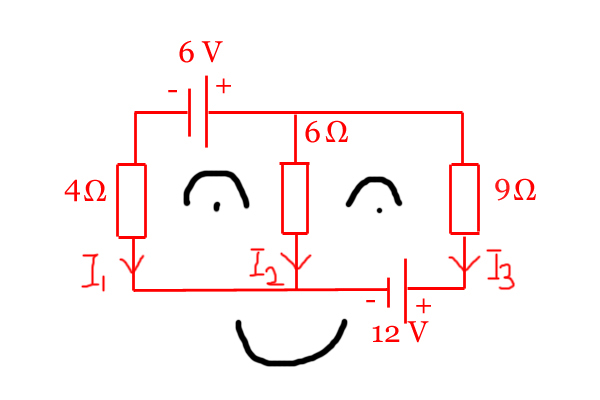
\includegraphics[scale = 0.4]{circuit.jpg}}
\caption{The circuit for Exercise \ref{ex:circuitsys}}
\label{fig:circuitsys}
\end{figure}\\
You will obtain two equations by considering any two loops with Kirchhoff’s Second Law, and one from Kirchhoff's First Law. So, there are three equations, for the three unknown currents.
\end{Exercise}
\begin{Answer}
The first two equations below come from the left inner loop and right inner loop, but one of them can be replaced by the outer loop as well.
\begin{align*}
-4I_1 + 6I_2 &= 6\\
-6I_2 + 9I_3 &= -12\\
I_1 + I_2 + I_3 &= 0
\end{align*}
and the solution is $I_1 = -\frac{3}{19}$, $I_2 = \frac{17}{19}$, $I_3 = -\frac{14}{19}$ (in Amperes).
\end{Answer}

\begin{Exercise}
\label{ex:shallowwater}
The \textit{shallow water equations} (see Figure \ref{fig:shallowwater}) describe the evolution of gravity wave under some approximations such as \textit{hydrostatic balance} and a sufficiently shallow fluid depth, and has the form of
\begin{align*}
\begin{dcases}
\frac{\partial \eta}{\partial t} + H(\frac{\partial u}{\partial x} + \frac{\partial v}{\partial y}) &= 0 \\
\frac{\partial u}{\partial t} &= -g\frac{\partial \eta}{\partial x} \\
\frac{\partial v}{\partial t} &= -g\frac{\partial \eta}{\partial y} 
\end{dcases}
\end{align*}
when the Coriolis effect is ignored. By assuming a travelling wave solution
\begin{align*}
u &= \tilde{U} \cos(kx + ly - \omega t) \\
v &= \tilde{V} \cos(kx + ly - \omega t) \\
\eta &= \tilde{\eta} \cos(kx + ly - \omega t)
\end{align*}
where $\tilde{U}$, $\tilde{V}$, $\tilde{\eta}$ are some constants to be determined, show that the equations become
\begin{align*}
\begin{dcases}
\omega \tilde{\eta} - kH \tilde{U} - lH \tilde{V} &= 0 \\
\omega \tilde{U} - kg \tilde{\eta} &= 0 \\
\omega \tilde{V} - lg \tilde{\eta} &= 0
\end{dcases}
\end{align*}
By requiring that $\tilde{U}$, $\tilde{V}$, $\tilde{\eta}$ have a non-trivial solution so that they are not all zeros, derive the dispersion relation of gravity wave, which is
\begin{align*}
\omega^2 &= gH(k^2 + l^2) \\
\omega &= c\kappa
\end{align*}
where $c = \sqrt{gH}$ is the wave speed, and $\kappa = \sqrt{k^2 + l^2}$ is the total wavenumber.
\end{Exercise}
\begin{figure}
\centering
\begin{tikzpicture}
    \draw [thick,color=black,domain=0:3*pi,samples=500] plot (\x, {5+0.5*sin(deg(4*\x))});
    \fill [blue!30] (3*pi,0) -- (0,0) -- plot[domain=0:3*pi,samples=500]  (\x, {5+0.5*sin(deg(4*\x))});
    \draw [thick,color=black] (0,0) -- (3*pi, 0);
    \fill [Brown!50!Orange] (0,0) rectangle (3*pi, -1) node[above left, black]{Bottom};
    \draw [<->] (3*pi+0.2, 0) -- (3*pi+0.2, 5) node[midway, xshift=8]{$H$};
    \draw [<->,red] (0.575*pi, 5.6) -- (0.575*pi, 5) node[midway, xshift=-8]{$\eta$};
    \draw [dashed, black] (0, 5) -- (3*pi, 5);
    \draw [thick, Green] (0.575*pi, 5) -- (0.575*pi, 0) node[midway, xshift=-8]{$u$};
    \draw [thick, Green, ->] (0.575*pi, 4) -- (0.575*pi+1, 4);
    \draw [thick, Green, ->] (0.575*pi, 3) -- (0.575*pi+1, 3);
    \draw [thick, Green, ->] (0.575*pi, 2) -- (0.575*pi+1, 2);
    \draw [thick, Green, ->] (0.575*pi, 1) -- (0.575*pi+1, 1);
    \node at (8.75, 2.5) {Fluid};
\end{tikzpicture}
\caption{The $x$-$z$ cross-section of shallow water system in Exercise \ref{ex:shallowwater}. $\eta$ is the height of free surface, $H$ is the mean depth of the fluid, and $u$ is the fluid velocity along $x$-axis.}
\label{fig:shallowwater}
\end{figure}
\begin{Answer}
Substituting the given wave solution forms into the equation, we have
\begin{align*}
\begin{split}
&\omega\tilde{\eta}\sin(kx+ly-\omega t) + H(-k\tilde{U}\sin(kx+ly-\omega t) \\
& -l\tilde{V}\sin(kx+ly-\omega t)) = 0 \\    
\end{split} \\
& \omega\tilde{U}\sin(kx+ly-\omega t) = gk\tilde{\eta}\sin(kx+ly-\omega t) \\
& \omega\tilde{V}\sin(kx+ly-\omega t) = gl\tilde{\eta}\sin(kx+ly-\omega t)
\end{align*}
Cancelling out all the sine factors, we arrive at the linear system displayed in the question
\begin{align*}
\begin{dcases}
\omega \tilde{\eta} - kH \tilde{U} - lH \tilde{V} &= 0 \\
\omega \tilde{U} - kg \tilde{\eta} &= 0 \\
\omega \tilde{V} - lg \tilde{\eta} &= 0
\end{dcases}
\end{align*}
For $\tilde{U}$, $\tilde{V}$, $\tilde{\eta}$ to have a non-trivial solution other than all zeros, we require the determinant of the corresponding coefficient matrix to be zero according to Theorem \ref{thm:sqlinsysunique}, which leads to
\begin{align*}
\begin{vmatrix}
\omega & -kH & -lH \\
-kg & \omega & 0 \\
-lg & 0 & \omega
\end{vmatrix} &= 0 \\
\omega^3 - gHk^2\omega - gHl^2\omega &= 0 \\
\omega^2 - gH(k^2 + l^2) &= 0 
\end{align*}
as the dispersion relation of gravity wave.
\end{Answer}

\begin{Exercise}
Solve for the condensation height and temperature $z_{cd}$ and $T_{cd}$ in Exercise \ref{ex:lapse}.
\end{Exercise}
\begin{Answer}
$T_{cd} \approx \SI{15.9}{\celsius}$, $z_{cd} \approx \SI{0.97}{\km}$.
\end{Answer}

\begin{Exercise}
Solve the \textit{Chickens and Rabbits in the Same Cage} problem in Exercise \ref{ex:animals}. If we now introduce a new type of mystical creature who has one head and three legs, and throw them in another cage along with some chickens and rabbits, find all possible numbers of the three species if the cage now has $48$ heads and $122$ legs.
\end{Exercise}
\begin{Answer}
$x = 23$, $y = 12$. For the extra part, the new system of equations become (denote the number of third species as $z$)
\begin{align*}
\begin{bmatrix}
1 & 1 & 1 \\
2 & 4 & 3
\end{bmatrix}
\begin{bmatrix}
x \\
y \\
z
\end{bmatrix}
=
\begin{bmatrix}
48 \\
122
\end{bmatrix}
\end{align*}
By Gaussian Elimination, we have
\begin{align*}
\left[
\begin{array}{@{}ccc|c@{}}
1 & 1 & 1 & 48 \\
2 & 4 & 3 & 122
\end{array}
\right]
&\to
\left[
\begin{array}{@{}ccc|c@{}}
1 & 1 & 1 & 48 \\
0 & 2 & 1 & 26
\end{array}
\right] & R_2 - 2R_1 \to R_2 \\
&\to
\left[
\begin{array}{@{}ccc|c@{}}
1 & 1 & 1 & 48 \\
0 & 1 & \frac{1}{2} & 13
\end{array}
\right] & \frac{1}{2}R_2 \to R_2 \\
&\to
\left[
\begin{array}{@{}ccc|c@{}}
1 & 0 & \frac{1}{2} & 35 \\
0 & 1 & \frac{1}{2} & 13
\end{array}
\right] & R_1 - R_2 \to R_1
\end{align*}
Let $z = t$ as the free variable, then we have $y = 13 - \frac{1}{2}t$ and $x = 35-\frac{1}{2}t$, and hence
\begin{align*}
\begin{bmatrix}
x \\
y \\
z
\end{bmatrix}
=
\begin{bmatrix}
35-\frac{1}{2}t \\
13-\frac{1}{2}t \\
t
\end{bmatrix}
=
\begin{bmatrix}
35 \\
13 \\
0
\end{bmatrix}
+
t
\begin{bmatrix}
-\frac{1}{2} \\
-\frac{1}{2} \\
1
\end{bmatrix}
\end{align*}
Since the numbers of species must be a non-negative integer, the solution can be expressed in a more good-looking form of
\begin{align*}
\begin{bmatrix}
x \\
y \\
z
\end{bmatrix}
=
\begin{bmatrix}
35 \\
13 \\
0
\end{bmatrix}
+
s
\begin{bmatrix}
-1 \\
-1 \\
2
\end{bmatrix}
\end{align*}
where $s = \frac{t}{2}$, and the range of $s$ is $0, 1, \ldots, 13$ (when $s$ reaches $13$ there is no chicken remained).
\end{Answer}
\chapter{Introduction to Vectors}

After three chapters of discussion about matrices, it is time to talk about another closely related object type in linear algebra, namely, vectors. While \textit{vectors} and \textit{vector spaces} have strictly mathematical definitions which make them abstract, we will take a more physical point of view with the special case of (finite-dimensional) geometric vectors first.

\section{Definition and Operations of Geometric Vectors}

\subsection{Basic Structure of Vectors in the Real $n$-space $\mathbb{R}^n$}
A \index{Vector}\index{Vector!Geometric Vector}\keywordhl{(geometric) vector} is a physical quantity represented by an ordered tuple of \textit{components} (numbers), e.g. $(1, 8, 7, 4)$, $(1-\imath, 1+3\imath, 2)$. It has a \textit{magnitude (length)} and \textit{direction}, resembling an arrow. Some real-life examples are: two-dimensional flow velocity $(u, v)$, the relative position of an airplane to a ground radar $(x, y, z)$.
\begin{defn}[$n$-dimensional Geometric Vector]
\label{defn:geometvec}
A $n$-dimensional geometric vector consists of $n$ ordered numbers called \index{Components}\keywordhl{components} and are denoted by either an arrow or boldface, like $\vec{v}$ or $\textbf{v}$. It is usually written out in two forms, as a \textit{column vector} or an \textit{ordered $n$-tuple}:
\begin{align*}
\vec{v} &=
\begin{bmatrix}
v_1 \\
v_2 \\
v_3 \\
\vdots \\
v_n
\end{bmatrix}
=
(v_1, v_2, v_3, \ldots, v_n)^T
\end{align*}
\end{defn}
A $n$-dimensional vector can be treated as an $n \times 1$ (\index{Vector!Column Vector}\keywordhl{column vector}) as suggested above, or a $1 \times n$ matrix (\index{Vector!Row Vector}\keywordhl{row vector}) depending on the situation. The form of a column vector is taken more often than the row vector one and so the column form is assumed throughout the book if it is not further specified. That is why the superscript $^T$ is added for the $n$-tuple form to reflect that it is in fact a column vector despite written horizontally. \par
\begin{tikzpicture}
\draw[->] (-2.5,0)--(2.5,0) node[right]{$x$};
\draw[->] (0,-2.5)--(0,2.5) node[above]{$y$};
\draw[blue,->,line width=1.2] (0,0)--(2,1) node[anchor=south]{$\vec{v} = (2,1)^T$};
\draw[Gray,dashed] (2,1)--(2,0) node[below]{$x = 2$};
\draw[Gray,dashed] (2,1)--(0,1) node[left]{$y = 1$};
\node[below left]{$O$}; 
\end{tikzpicture}\\    
A 2D vector drawn in an x-y plane.\par
{\fbox{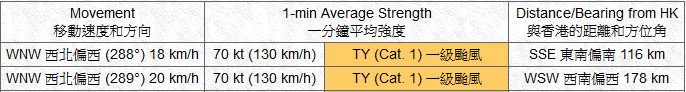
\includegraphics[scale = 0.5]{higos.jpg}}\\
Forecast for \textit{Typhoon Higos} (taken from \href{http://www.hkww.org/weather/tcarchive.html}{Hong Kong Weather Watch}). Its horizontal movement is a two-dimensional vector, even though the speed and direction are given instead of the velocities in $x$ and $y$-direction (they can be converted to each other).}

Implicit in the definition of $n$-dimensional vectors is the $n$-dimensional \textit{space} they are residing in. Assume the components of those vectors are all real, then the set of all such vectors constitutes the \index{Real $n$-space}\keywordhl{real $n$-space $\mathbb{R}^n$}.
\begin{defn}[The Real $n$-space $\mathbb{R}^n$]
\label{defn:real_nspace}
The real $n$-space $\mathbb{R}^n$ is defined as the set of all possible $n$-tuples $\vec{v} = (v_1, v_2, v_3, \ldots, v_n)^T$ as defined in Definition \ref{defn:geometvec}, where $v_i$ can take any \textit{real} value, for $i = 1,2,3,\ldots,n$. Such objects in $\mathbb{R}^n$ are known as $n$-dimensional \textit{real} vectors.
\end{defn}
While we have not clearly defined what a vector space is, we note that $\mathbb{R}^n$ fulfills the requirements of a vector space in a mathematical sense. A more detailed discussion of this aspect will be deferred to Chapter \ref{chap:vec_space}. Meanwhile, the complex counterpart will be explored in Chapter \ref{chap:complex}.\\
\\
An $n$-dimensional real geometric vector as described in Definition \ref{defn:geometvec} and \ref{defn:real_nspace} can be written as the sum of $n$ \index{Standard Unit Vector}\keywordhl{standard unit vectors} that have a magnitude of $1$ and are oriented in the positive direction along the $p$-th coordinates axes. They are denoted by $\hat{e}_p$, where $p$ can be from $1$ to $n$. The coordinate axes are perpendicular (or more generally, \textit{orthogonal}, introduced later in this chapter) to each other and this coordinate system is known as the \index{Cartesian Coordinate System}\keywordhl{Cartesian (coordinate) system}. Particularly, in the three-dimensional real space $\mathbb{R}^3$, $\hat{e}_1 = \hat{i} = (1,0,0)^T$, $\hat{e}_2 = \hat{j} = (0,1,0)^T$, $\hat{e}_3 = \hat{k} = (0,0,1)^T$ correspond to "an arrow" of length $1$ pointing in the positive direction of the $x$, $y$, $z$ axes respectively. 
\begin{defn}[Standard Unit Vector]
\label{defn:standardunitvec}
A standard unit vector $\hat{e}_p$ in the real $n$-space $\mathbb{R}^n$ (Definition \ref{defn:real_nspace}) has $n$ components, consisted of $1$ at the $p$-th entry and $0$ elsewhere. Mathematically, for $1\leq q \leq n$, $[\hat{e}_p]_q = 1$ when $q=p$ and $[\hat{e}_p]_q = 0$ when $q\neq p$.
\end{defn}
Below is an example of a geometric vector in the three-dimensional $xyz$ space ($\mathbb{R}^3$).
\begin{center}
\begin{tikzpicture}[x={(1.8cm, -0.4cm)}, y={(1.4cm, 1.2cm)}, z={(0cm, 2cm)}]
\draw [->] (0,0,0) -- (2,0,0) node [below right] {$x$};
\draw [->] (0,0,0) -- (0,2,0) node [above] {$y$};
\draw [->] (0,0,0) -- (0,0,2) node [left] {$z$};
\draw [->, thick, red, line width=1] (0,0,0) -- (1,0,0) node [below left] {$\hat{i} = (1,0,0)^T$};
\draw [->, thick, red, line width=1] (0,0,0) -- (0,1,0) node [above right, midway, sloped] {$\hat{j} = (0,1,0)^T$} ; 
\draw [->, thick, red, line width=1] (0,0,0) -- (0,0,1) node [left] {$\hat{k} = (0,0,1)^T$};
\draw [Gray, dashed] (1.8,0.4,0) -- (1.8,0,0) node[right, midway]{$y=0.4$}; 
\draw [Gray, dashed] (1.8,0.4,0) -- (0,0.4,0) node[above, midway, sloped]{$x=1.8$}; 
\draw [Gray, dashed] (1.8,0.4,0) -- (1.8,0.4,1.1) node[midway, right]{$z=1.1$};
\draw [->, blue, line width=1.2] (0,0,0) -- (1.8,0.4,1.1) node [right] {$\vec{v} = (1.8,0.4,1.1)^T$};
/\end{tikzpicture}
\begin{align*}
\vec{v} &= 
\begin{bmatrix}
1.8 \\
0.4 \\
1.1
\end{bmatrix}
= 1.8
\begin{bmatrix}
1 \\
0 \\
0
\end{bmatrix}
+ 0.4
\begin{bmatrix}
0 \\
1 \\
0
\end{bmatrix}
+ 1.1
\begin{bmatrix}
0 \\
0 \\
1
\end{bmatrix} 
= 1.8\hat{i} + 0.4\hat{j} + 1.1\hat{k} \\
&= (1.8,0.4,1.1)^T
\end{align*}
\end{center}
where we have written $\vec{v}$ in two forms, as an $n$-tuple and a sum of the three standard unit vectors $\hat{i}, \hat{j}, \hat{k}$.

\subsection{Fundamental Vector Operations}
\label{section:vectoraddmul}
\subsubsection{Addition and Subtraction}
Same as their matrix counterpart, addition and subtraction between vectors are component-wise, and hence only valid for vectors of the same dimension. For $\vec{w} = \vec{u} \pm \vec{v}$, we have $w_i = u_i \pm v_i$. If
\begin{align*}
&\vec{u} =
\begin{bmatrix}
1 \\
2
\end{bmatrix}
&
\vec{v} =
\begin{bmatrix}
2 \\
-1
\end{bmatrix}
\end{align*}
then
\begin{align*}
\vec{u} + \vec{v} =
\begin{bmatrix}
\textcolor{red}{1} \\
\textcolor{red}{2}
\end{bmatrix}
+
\begin{bmatrix}
\textcolor{blue}{2} \\
\textcolor{blue}{-1}
\end{bmatrix}
&= 
\begin{bmatrix}
\textcolor{Green}{3} \\
\textcolor{Green}{1}
\end{bmatrix}
\\
\vec{u} - \vec{v} =
\begin{bmatrix}
\textcolor{red}{1} \\
\textcolor{red}{2}
\end{bmatrix}
-
\begin{bmatrix}
\textcolor{blue}{2} \\
\textcolor{blue}{-1}
\end{bmatrix}
&= 
\begin{bmatrix}
\textcolor{Green}{-1} \\
\textcolor{Green}{3}
\end{bmatrix}
\end{align*}
\begin{center}
\begin{tikzpicture}[scale=0.8]
\draw[->] (-3.5,0)--(3.5,0) node[right]{$x$};
\draw[->] (0,-3.5)--(0,3.5) node[above]{$y$};
\draw[red,-stealth,line width=1] (0,0)--(1,2) node[anchor=south west]{$\vec{u} = (1,2)^T$};
\draw[blue,-stealth,line width=1] (1,2)--(3,1) node[anchor=south west]{$\vec{v} = (2,-1)^T$};
\draw[Green,-stealth,line width=1] (0,0)--(3,1) node[anchor=north west]{$\vec{u} + \vec{v} = (3,1)^T$};
\node[below left]{$O$}; 
\end{tikzpicture}\\
Addition: The tail of the blue vector is placed to the head of the red vector, and the resultant green vector is from the origin to the head of blue vector.
\end{center}
\begin{center}
\begin{tikzpicture}[scale=0.8]
\draw[->] (-3.5,0)--(3.5,0) node[right]{$x$};
\draw[->] (0,-3.5)--(0,3.5) node[above]{$y$};
\draw[red,-stealth,line width=1] (0,0)--(1,2) node[anchor=south west]{$\vec{u} = (1,2)^T$};
\draw[blue,-stealth,line width=1] (1,2)--(-1,3) node[anchor=south east]{$-\vec{v} = (-2,1)^T$};
\draw[Green,-stealth,line width=1] (0,0)--(-1,3) node[anchor=north east]{$\vec{u} - \vec{v} = (-1,3)^T$};
\node[below left]{$O$}; 
\end{tikzpicture}\\
Subtraction: Similar to addition but with the blue vector oriented in the opposite direction.
\end{center}

\subsubsection{Scalar Multiplication} 
Multiplying a scalar (be it a real or complex number) to a vector means that all components are multiplied by that scalar.
\begin{align*}
2
\begin{bmatrix}
2 \\
0 \\
1 \\
9
\end{bmatrix}
=
\begin{bmatrix}
4 \\
0 \\
2 \\
18
\end{bmatrix}
\end{align*}
Looking back at vector subtraction, it can be viewed as addition with a factor of $-1$ in the front.
\begin{align*}
\begin{bmatrix}
7 \\
5 \\
9
\end{bmatrix}
-
\begin{bmatrix}
3 \\
6 \\
9
\end{bmatrix}
=
\begin{bmatrix}
7 \\
5 \\
9
\end{bmatrix}
+ (-1)
\begin{bmatrix}
3 \\
6 \\
9
\end{bmatrix}
=
\begin{bmatrix}
7 \\
5 \\
9
\end{bmatrix}
+
\begin{bmatrix}
-3 \\
-6 \\
-9
\end{bmatrix}
=
\begin{bmatrix}
4 \\
-1 \\
0
\end{bmatrix}
\end{align*}

\subsubsection{Length and Unit Vector} \index{Length}\index{Magnitude}\keywordhl{Length (magnitude)}, or more formally \index{Euclidean Norm}\keywordhl{Euclidean norm}, of a vector $\vec{v}$ is based on a generalized version of \index{Pythagoras' Theorem}\keywordhl{Pythagoras' Theorem}, and is evaluated as the square root of the sum of squares of components.
\begin{defn}[Vector Length]
\label{defn:vectorlength}
Length, or magnitude of a $n$-dimensional \textit{real} vector $\vec{v}$, denoted by $\norm{\vec{v}}$, is given by
\begin{align*}
\norm{\vec{v}} &= \sqrt{v_1^2 + v_2^2 + v_3^2 + \cdots + v_n^2} \\
&= \sqrt{\sum_{k=1}^{n} v_k^2}
\end{align*}
\end{defn}
For instance, the length of a two-dimensional vector follows the usual Pythagoras' Theorem as below. \\
\begin{tikzpicture}
\draw[->] (-2.5,0)--(2.5,0) node[right]{$x$};
\draw[->] (0,-2.5)--(0,2.5) node[above]{$y$};
\draw[blue,-stealth,line width=1.2] (0,0)--(2,1) node[anchor=south west, align=left]{$\vec{v} = (2,1)^T$\\$\norm{\vec{v}} = \sqrt{x^2 + y^2} = \sqrt{2^2+1^2} = \sqrt{5}$};
\draw[Gray,dashed] (2,1)--(2,0) node[below]{$x = 2$};
\draw[Gray,dashed] (2,1)--(0,1) node[left]{$y = 1$};
\node[below left]{$O$}; 
\end{tikzpicture}\\
Here is another example which is three-dimensional.
\begin{center}
\begin{tikzpicture}[x={(1.8cm, -0.6cm)}, y={(1.6cm, 1.0cm)}, z={(0cm, 2cm)}]
\draw [->] (-1,0,0) -- (2,0,0) node [right] {$x$};
\draw [->] (0,-1,0) -- (0,2,0) node [above] {$y$};
\draw [->] (0,0,0) -- (0,0,2) node [left] {$z$};
\node[below] (0,0,0){$O$};
\draw [Gray, dashed] (1.6,-0.2,0) -- (1.6,0,0) node[below, pos=-0.5, sloped]{$y=-1$}; 
\draw [Gray, dashed] (1.6,-0.2,0) -- (0,-0.2,0) node[below, midway, sloped]{$x=8$}; 
\draw [Gray, dashed] (1.6,-0.2,0) -- (1.6,-0.2,0.8) node[midway, right]{$z=4$};
\draw [->, blue, line width=1.2] (0,0,0) -- (1.6,-0.2,0.8) node [right] {$\vec{w} = (8,-1,4)^T$};
\end{tikzpicture}
\begin{align*}
\vec{w} &= 
\begin{bmatrix}
8 \\
-1 \\
4
\end{bmatrix}
& \norm{\vec{w}}&=
\sqrt{8^2 + (-1)^2 + 4^2} = 9 
\end{align*}
\end{center}
We can create a \index{Vector!Unit Vector}\keywordhl{unit vector} that has a length of $1$ from any vector $\vec{v}$ and orients in the same direction as $\vec{v}$. It is simply created by dividing (normalizing) $\vec{v}$ by its distance $\norm{\vec{v}}$.
\begin{defn}[Unit Vector]
\label{defn:unitvec}
The unit vector corresponding to a non-zero vector $\vec{v}$ is denoted as $\hat{v}$ and is given by
\begin{align*}
\hat{v} &= \frac{1}{\norm{\vec{v}}}\vec{v}
\end{align*}
where the length $\norm{\vec{v}}$ is defined as in Definition \ref{defn:vectorlength}. 
\end{defn}
Note that despite vectors can carry physical units, unit vectors are all physically \textit{dimensionless} when formulated in this way. \\
\\
Short Exercise: Find the unit vector for $\vec{w} = (8, -1, 4)^T$ in the previous example, and verify that it has a length of $1$.\footnote{$\norm{\vec{w}} = 9$, $\hat{w} = \frac{\vec{w}}{\norm{\vec{w}}} = \frac{1}{9}(8,-1,4)^T = (\frac{8}{9}, -\frac{1}{9}, \frac{4}{9})^T$, $\norm{\hat{w}} = \sqrt{(\frac{8}{9})^2 + (-\frac{1}{9})^2 + (\frac{4}{9})^2} = 1$.}

\section{Special Vector Operations}
\label{section:vectorops}
Now we are going to introduce two special types of vector operations: \textit{dot product}, and \textit{cross product}. 

\subsection{Dot Product}
\label{section:dotprod}
\index{Dot Product}\keywordhl{(Real) Dot product} (or \index{Scalar Product}\keywordhl{scalar product}) is defined for two (real) vectors that have the same number of dimension. It is the sum of products of paired components between the two vectors. In other words, it can be regarded to be the matrix product between a row vector ($1 \times m$ matrix) and a column vector ($m \times 1$ matrix). 
\begin{defn}[Dot Product (Real)]
\label{defn:dotreal}
The dot product between two $n$-dimensional \textit{real} vectors $\vec{u}$ and $\vec{v}$ in $\mathbb{R}^n$ are denoted as either $\vec{u} \cdot \vec{v}$, or by matrix notation $\textbf{u}^T\textbf{v}$. They are defined as
\begin{align*}
\vec{u} \cdot \vec{v} = \textbf{u}^T\textbf{v} &= u_1v_1 + u_2v_2 + u_3v_3 + \cdots + u_nv_n \\
&= \sum_{k=1}^{n} u_kv_k
\end{align*}
which is a scalar quantity.
\end{defn}
Conversely, it can be said that entries of a matrix product are vector dot products between the corresponding rows and columns. It is emphasized that we are restricting ourselves to real entries since complex vectors introduce a bit of extra complications. Then, for two \textit{real} matrices expressed in the form of combined row/column vectors that are $\mathbb{R}^n$,
\begin{align*}
A &= \left[\begin{array}{@{}c@{}}
\text{---} \vec{u}^{(1)T} \text{---} \\
\hline
\text{---} \vec{u}^{(2)T} \text{---} \\
\hline
\vdots \\
\hline
\text{---} \vec{u}^{(p)T} \text{---}
\end{array}\right]
=  \left[\begin{array}{@{}c|c|c|c@{}}
| & | & & | \\
\vec{u}^{(1)} & \vec{u}^{(2)} & \cdots & \vec{u}^{(p)} \\
| & | & & |
\end{array}\right]^T
& B &= \left[\begin{array}{@{}c|c|c|c@{}}
| & | & & | \\
\vec{v}^{(1)} & \vec{v}^{(2)} & \cdots & \vec{v}^{(q)} \\
| & | & & |
\end{array}\right]\\
&= 
\begin{bmatrix}
\vec{u}^{(1)}_1  & \vec{u}^{(1)}_2 & \cdots & \vec{u}^{(1)}_n \\
\vec{u}^{(2)}_1  & \vec{u}^{(2)}_2 & \cdots & \vec{u}^{(2)}_n \\
\vdots & \vdots & & \vdots \\
\vec{u}^{(p)}_1  & \vec{u}^{(p)}_2 & \cdots & \vec{u}^{(p)}_n
\end{bmatrix} 
& &= 
\begin{bmatrix}
\vec{v}^{(1)}_1  & \vec{v}^{(2)}_1 & \cdots & \vec{v}^{(q)}_1 \\
\vec{v}^{(1)}_2  & \vec{v}^{(2)}_2 & & \vec{v}^{(q)}_2 \\
\vdots & & \ddots & \vdots \\
\vec{v}^{(1)}_n  & \vec{v}^{(2)}_n & \cdots & \vec{v}^{(q)}_n \\
\end{bmatrix} 
\end{align*}
(notice those transposes in the expression of $A$) their matrix product $AB$ can be written as
\begin{align*}
AB =
\begin{bmatrix}
\vec{u}^{(1)} \cdot \vec{v}^{(1)} & \vec{u}^{(1)} \cdot \vec{v}^{(2)} & \cdots & \vec{u}^{(1)} \cdot \vec{v}^{(q)} \\
\vec{u}^{(2)} \cdot \vec{v}^{(1)} & \vec{u}^{(2)} \cdot \vec{v}^{(2)} & \cdots & \vec{u}^{(2)} \cdot \vec{v}^{(q)} \\
\vdots & \vdots & & \vdots \\
\vec{u}^{(p)} \cdot \vec{v}^{(1)} & \vec{u}^{(p)} \cdot \vec{v}^{(2)} & \cdots & \vec{u}^{(p)} \cdot \vec{v}^{(q)} \\
\end{bmatrix}
\end{align*}
We can use dot product to express the length of a real vector.
\begin{proper}
\label{proper:lengthdot}
The length of a real vector, as defined in Definition \ref{defn:vectorlength}, can be written using its dot product between itself as
\begin{align*}
\norm{\vec{v}} &= \sqrt{\vec{v} \cdot \vec{v}} & &\text{or} &
\norm{\vec{v}}^2 &= \vec{v} \cdot \vec{v}
\end{align*}
\end{proper}
Notice that $\vec{v} \cdot \vec{v} = v_1^2 + v_2^2 + v_3^2 + \cdots + v_n^2 \geq 0$. This quantity is always strictly greater than zero ($\vec{v} \cdot \vec{v} > 0$) unless $\vec{v} = \textbf{0}$ is the zero vector (then $\vec{v} \cdot \vec{v} = 0$), which makes sense physically given that it represents length.

\begin{exmp}
\label{exmp:dotproduct5d}
If $\vec{u} = (1, 2, 3, 4, 5)^T$ and $\vec{v} = (-1, 0, 2, 1, -2)^T$, find the dot product $\vec{u} \cdot \vec{v} = \textbf{u}^T\textbf{v}$.
\end{exmp}
\begin{solution}
\begin{align*}
\vec{u} \cdot \vec{v} &= (1)(-1) + (2)(0) + (3)(2) + (4)(1) + (5)(-2) = -1
\end{align*}
Alternatively,
\begin{align*}
\textbf{u}^T\textbf{v} &=
\begin{bmatrix}
1 & 2 & 3 & 4 & 5
\end{bmatrix}
\begin{bmatrix}
-1 \\
0 \\
2 \\
1 \\
-2
\end{bmatrix}
= -1
\end{align*}
\end{solution}

Here are some properties of dot product.
\begin{proper}
\label{proper:dotproper}
For three $n$-dimensional real vectors $\vec{u}$, $\vec{v}$ and $\vec{w}$, the following properties hold.
\begin{align*}
\vec{u} \cdot \vec{v} &= \vec{v} \cdot \vec{u} &\text{Symmetry Property} \\
\vec{u} \cdot (\vec{v} \pm \vec{w}) &= \vec{u} \cdot \vec{v} \pm \vec{u} \cdot \vec{w} &\text{Distributive Property} \\
(\vec{u} \pm \vec{v}) \cdot \vec{w} &= \vec{u} \cdot \vec{w} \pm \vec{v} \cdot \vec{w} &\text{Distributive Property} \\
(a\vec{u}) \cdot (b\vec{v}) &= ab(\vec{u} \cdot \vec{v}) &\text{where $a$, $b$ are some constants}
\end{align*}
Additionally, if $A$ is an $n \times n$ square matrix, then
\begin{align*}
\vec{u} \cdot (A\vec{v}) &= \textbf{u}^T(A\textbf{v}) = (A^T\textbf{u})^T\textbf{v} = (A^T\vec{u}) \cdot \vec{v} \\
(A\vec{u}) \cdot \vec{v} &= (A\textbf{u})^T\textbf{v} = \textbf{u}^T(A^T\textbf{v}) = \vec{u} \cdot (A^T\vec{v})
\end{align*}
where we have used Definition \ref{defn:dotreal} and Properties \ref{proper:transp}.
\end{proper}
\begin{exmp}
For $\vec{u} = (1,3,1)^T$ and $\vec{v} = (2,-1,1)^T$, find $\norm{(\vec{u} + \vec{v})}^2 = (\vec{u} + \vec{v}) \cdot (\vec{u} + \vec{v})$.
\end{exmp}
\begin{solution}
By Properties \ref{proper:dotproper}, we can rewrite the expression as
\begin{align*}
(\vec{u} + \vec{v}) \cdot (\vec{u} + \vec{v}) &= \vec{u} \cdot (\vec{u} + \vec{v}) + \vec{v} \cdot (\vec{u} + \vec{v}) \\
&= \vec{u} \cdot \vec{u} + \vec{u} \cdot \vec{v} + \vec{v} \cdot \vec{u} + \vec{v} \cdot \vec{v} \\
&= \vec{u} \cdot \vec{u} + 2 \vec{u} \cdot \vec{v} + \vec{v} \cdot \vec{v}
\end{align*}
Subsequently,
\begin{align*}
&\quad \vec{u} \cdot \vec{u} + 2 \vec{u} \cdot \vec{v} + \vec{v} \cdot \vec{v} \\
&= (1,3,1)^T \cdot (1,3,1)^T + 2((1,3,1)^T \cdot (2,-1,1)^T) + (2,-1,1)^T \cdot (2,-1,1)^T \\
&= (1^2 + 3^2 + 1^2) + 2((1)(2)+(3)(-1)+(1)(1)) + (2^2 + (-1)^2 + 1^2) \\
&= 11 + 2(0) + 6 \\
&= 17
\end{align*}
Alternatively, one can calculate $\vec{w} = \vec{u} + \vec{v} = (1,3,1)^T + (2,-1,1)^T = (3,2,2)^T$ and find $\vec{w} \cdot \vec{w} = \norm{\vec{w}}^2$ instead. (which is easier and faster)
\end{solution}
\begin{exmp}
Given $\vec{u}$ and $\vec{v}$ as defined in the example above, if
\begin{align*}
A =
\begin{bmatrix}
1 & 2 & 1 \\
2 & 0 & 3 \\
1 & 1 & -1
\end{bmatrix}
\end{align*}
verify that $\vec{u} \cdot (A\vec{v}) = (A^T\vec{u}) \cdot \vec{v}$.
\end{exmp}
\begin{solution}
\begin{align*}
A\vec{v} &= 
\begin{bmatrix}
1 & 2 & 1 \\
2 & 0 & 3 \\
1 & 1 & -1
\end{bmatrix}
\begin{bmatrix}
2 \\
-1 \\
1
\end{bmatrix} \\
&=
\begin{bmatrix}
(1)(2) + (2)(-1) + (1)(1) \\
(2)(2) + (0)(-1) + (3)(1) \\
(1)(2) + (1)(-1) + (-1)(1) 
\end{bmatrix} \\
&=
\begin{bmatrix}
1 \\
7 \\
0
\end{bmatrix} \\
\vec{u} \cdot (A\vec{v}) &= (1,3,1)^T \cdot (1,7,0)^T \\
&= (1)(1) + (3)(7) + (1)(0) \\
&= 22
\end{align*}
On the other hand,
\begin{align*}
A^T\vec{u} &= 
\begin{bmatrix}
1 & 2 & 1 \\
2 & 0 & 1 \\
1 & 3 & -1
\end{bmatrix}
\begin{bmatrix}
1 \\
3 \\
1
\end{bmatrix} \\
&=
\begin{bmatrix}
(1)(1) + (2)(3) + (1)(1) \\
(2)(1) + (0)(3) + (1)(1) \\
(1)(1) + (3)(3) + (-1)(1) 
\end{bmatrix} \\
&=
\begin{bmatrix}
8 \\
3 \\
9
\end{bmatrix} \\
(A^T\vec{u}) \cdot \vec{v} &= (8,3,9)^T \cdot (2,-1,1)^T \\
&= (8)(2) + (3)(-1) + (9)(1) \\
&= 22
\end{align*}
\end{solution}

\subsubsection{Geometric Meaning of Dot Product}
The geometric meaning of dot product is embedded in the relation below.
\begin{proper}
\label{proper:dotgeo}
For two real vectors $\vec{u}$ and $\vec{v}$ that are of the same dimension, we have
\begin{align*}
\vec{u} \cdot \vec{v} = \norm{\vec{u}}\norm{\vec{v}}\cos\theta
\end{align*}
where $\theta$ is the angle between $\vec{u}$ and $\vec{v}$. Furthermore, if $\hat{u}$ and $\hat{v}$ are unit vectors (Definition \ref{defn:unitvec}) such that $\norm{\vec{u}} = \norm{\vec{v}} = 1$, it reduces to
\begin{align*}
\hat{u} \cdot \hat{v} = \cos\theta    
\end{align*}
\end{proper}
This means that the dot product between two vectors $\vec{u}$ and $\vec{v}$ is geometrically the signed product between $\vec{u}$ and the parallel component (projection) of $\vec{v}$ onto $\vec{u}$ (or vice versa), which is illustrated in the figure below. While an angle has a clear physical meaning only in a two/three-dimensional space, such relation generalizes the idea of an angle to higher dimensions.
\begin{center}
\begin{tikzpicture}[scale=1.3]
\coordinate (0) at (0,0);
\coordinate (vecu) at (4,1);
\coordinate (vecv) at (1,2);
\draw[->](0)--(vecu) node[right]{$\vec{u}$};
\draw[->](0)--(vecv) node[above]{$\vec{v}$};
\draw[dashed] (1,2)--(24/17, 6/17);
\draw[red] (24/17+0.2, 6/17+0.05)--(24/17+0.15, 6/17+0.25)--(24/17-0.05, 6/17+0.2);
\pic[draw, "$\theta$", angle eccentricity=1.5] {angle = vecu--0--vecv};
\draw[blue, very thick] (0,0)--(24/17, 6/17) node[below, shift={(0mm, -2mm)}]{$\norm{\vec{v}}\cos\theta$};
\end{tikzpicture}
\end{center}
\begin{exmp}
Find the angle between $\vec{u}$ and $\vec{v}$ in Example \ref{exmp:dotproduct5d}.
\end{exmp}
\begin{solution}
From Example \ref{exmp:dotproduct5d}, we have $\vec{u} \cdot \vec{v} = -1$, and
\begin{align*}
\norm{\vec{u}} &= \sqrt{1^2 + 2^2 + 3^2 + 4^2 + 5^2} = \sqrt{55} \\
\norm{\vec{v}} &= \sqrt{(-1)^2 + 0^2 + 2^2 + 1^2 + (-2)^2} = \sqrt{10} 
\end{align*}
By Properties \ref{proper:dotgeo}, we have
\begin{align*}
\cos\theta &= \frac{\vec{u} \cdot \vec{v}}{\norm{\vec{u}}\norm{\vec{v}}} \\
&= \frac{-1}{(\sqrt{55})(\sqrt{10})} \\
&\approx -0.0426 \\
\theta &\approx \SI{1.613}{\radian} = \SI{92.44}{\degree}
\end{align*}
\end{solution}
By Properties \ref{proper:dotgeo}, if the absolute value of the dot product $|\vec{u} \cdot \vec{v}|$ is equal to $\norm{\vec{u}}\norm{\vec{v}}$, where $\vec{u}$ and $\vec{v}$ are non-zero vectors, then it implies that $\cos\theta = \pm 1$, $\theta$ is either $0$ or $\pi$, and hence the two vectors are parallel. In constrast,
\begin{proper}
\label{proper:dotorth}
If the dot product between two real vectors $\vec{u}$ and $\vec{v}$ is zero ($\vec{u} \cdot \vec{v} = \vec{v} \cdot \vec{u} = 0$), then by Properties \ref{proper:dotgeo}, $\cos\theta = 0$ and the angle $\theta$ between $\vec{u}$ and $\vec{v}$ is $\frac{\pi}{2}$. In this case, $\vec{u}$ and $\vec{v}$ are said to be perpendicular, or \textit{orthogonal} to each other.
\end{proper}
From this, the concept of "\index{Orthogonal}\keywordhl{orthogonal}" becomes an extension of "perpendicular" in higher dimensions. It is easy to see that the standard unit vectors of $\mathbb{R}^n$ are orthogonal. Note that \textit{the zero vector is regarded to be orthogonal to any vector}, so even if $\vec{u}$ or $\vec{v}$ is a zero vector, this properties still hold. \par
Some may notice that as $-1 \leq \cos\theta \leq 1$, if $|\vec{u} \cdot \vec{v}| > \norm{\vec{u}}\norm{\vec{v}}$, then $\theta$ in Properties \ref{proper:dotgeo} will be ill-defined. However, the \index{Cauchy–Schwarz Inequality}\keywordhl{Cauchy–Schwarz Inequality} ensures this will not happen.
\begin{thm}[Cauchy–Schwarz Inequality]
\label{thm:CauchySch}
Given two \textit{real} $n$-dimensional vectors $\vec{u}$ and $\vec{v}$ ($\vec{u}, \vec{v} \in \mathbb{R}^n$), the following inequality holds.
\begin{align*}
|\vec{u} \cdot \vec{v}| &\leq \norm{\vec{u}}\norm{\vec{v}} \\
|u_1v_1+u_2v_2+\cdots+u_nv_n| &\leq \sqrt{u_1^2+u_2^2+\cdots+u_n^2}\sqrt{v_1^2+v_2^2+\cdots+v_n^2}
\end{align*}
\end{thm}
\begin{proof}
Consider $\vec{w} = \vec{u} + t\vec{v}$, where $t$ is any scalar, then $\norm{\vec{w}}^2 = \vec{w}\cdot\vec{w} \geq 0$ by Properties \ref{proper:lengthdot}. Also, $\vec{w}\cdot\vec{w}$ can be written as a quadratic polynomial in $t$:
\begin{align*}
\vec{w}\cdot\vec{w} = (\vec{u} + t\vec{v}) \cdot (\vec{u} + t\vec{v}) = \norm{\vec{u}}^2 + 2t(\vec{u} \cdot \vec{v}) + t^2\norm{\vec{v}}^2
\end{align*}
Since this quantity is always greater than or equal to zero, i.e.\ the quadratic polynomial has no root or a repeated root, it means that the discriminant must be negative or zero. So,
\begin{align*}
\Delta = b^2 - 4ac &\leq 0 \\
(2(\vec{u} \cdot \vec{v}))^2 - 4\norm{\vec{u}}^2\norm{\vec{v}}^2 &\leq 0 \\
(\vec{u} \cdot \vec{v})^2 - \norm{\vec{u}}^2\norm{\vec{v}}^2 &\leq 0 \\
(\vec{u} \cdot \vec{v})^2 &\leq \norm{\vec{u}}^2\norm{\vec{v}}^2 \\
|\vec{u} \cdot \vec{v}| &\leq \norm{\vec{u}}\norm{\vec{v}}
\end{align*}
\end{proof}
Short Exercise: Think about under what circumstances the Cauchy–Schwarz Inequality turns into an equality (i.e.\ $|\vec{u} \cdot \vec{v}| = \norm{\vec{u}}\norm{\vec{v}}$).\footnote{When $\vec{u}$ and $\vec{v}$ are parallel, i.e. $\vec{u} = k\vec{v}$ for some scalar $k$, or $\vec{v} = \textbf{0}$.}

\begin{exmp}
Prove the \index{Cosine Law}\keywordhl{Cosine Law} by considering the triangle below
\begin{center}
\begin{tikzpicture}
\coordinate (0) at (0,0);
\draw[red,-{Latex[length=5mm, width=2mm]}] (0)--(5,1) node[right](vecu){$\vec{u}$};
\draw[blue,-{Latex[length=5mm, width=2mm]}] (0)--(-1,3) node[above](vecv){$\vec{v}$};
\pic[draw, "$\theta$", angle eccentricity=1.5] {angle = vecu--0--vecv};
\draw[Green,-{Latex[length=5mm, width=2mm]}] (-1,3)--(5,1) node[midway, above, shift={(0mm, 3mm)}]{$\vec{u} - \vec{v}$};
\end{tikzpicture}
\end{center}
and expanding the dot product $\norm{(\vec{u}-\vec{v})}^2 = (\vec{u}-\vec{v}) \cdot (\vec{u}-\vec{v})$.    
\end{exmp}
\begin{solution}
Let denote the lengths $\norm{\vec{u}}$, $\norm{\vec{v}}$, $\norm{(\vec{u}-\vec{v})}$ be $a$, $b$, $c$, then
\begin{align*}
c^2 = \norm{(\vec{u}-\vec{v})}^2 &= (\vec{u}-\vec{v}) \cdot (\vec{u}-\vec{v}) & \text{(Properties \ref{proper:lengthdot})} \\
&= \vec{u} \cdot \vec{u} - \vec{u} \cdot \vec{v} - \vec{v} \cdot \vec{u} + \vec{v} \cdot \vec{v} & \text{(Properties \ref{proper:dotproper})} \\
&= \norm{\vec{u}}^2 - 2\vec{u} \cdot \vec{v} + \norm{\vec{v}}^2 & \text{(Properties \ref{proper:lengthdot} and \ref{proper:dotproper})} \\
&= \norm{\vec{u}}^2 - 2\norm{\vec{u}}\norm{\vec{v}}\cos\theta + \norm{\vec{v}}^2 & \text{(Properties \ref{proper:dotgeo})} \\
&= a^2 - 2ab\cos\theta + b^2
\end{align*}
\end{solution}

\subsection{Cross Product}
\label{section:crossprod}
Another important type of vector product is the \index{Cross Product}\keywordhl{cross product} (or sometimes just \index{Vector Product}\keywordhl{vector product}), which produces a three-dimensional real vector from two other three-dimensional real vectors. \textit{The output vector will be orthogonal to the two input vectors}, and the direction is determined by the \index{Right Hand Rule}\keywordhl{right hand rule}. Motivated by these requirements, we have the following basic definitions of cross product between the three standard unit vectors in $\mathbb{R}^3$.
\begin{defn}
\label{defn:crossijk}
The computation of cross products (denoted by $\times$) involving any two of the standard unit vectors $\hat{i}$, $\hat{j}$, $\hat{k}$ in $\mathbb{R}^3$ obeys the following rules.
\begin{enumerate}
\item $\hat{i} \times \hat{j} = \hat{k}$, $\hat{j} \times \hat{i} = -\hat{k}$,
\item $\hat{j} \times \hat{k} = \hat{i}$, $\hat{k} \times \hat{j} = -\hat{i}$,
\item $\hat{k} \times \hat{i} = \hat{j}$, $\hat{i} \times \hat{k} = -\hat{j}$, and
\item $\hat{i} \times \hat{i} = \hat{j} \times \hat{j} = \hat{k} \times \hat{k} = \textbf{0}$
\end{enumerate}
\end{defn}
\begin{minipage}{0.45\textwidth}
\begin{center}
% https://tex.stackexchange.com/questions/287284/drawing-a-diagram-of-a-three-cycle
\begin{tikzpicture}[->,scale=2]
   \node (i) at (90:1cm)  {\huge$\hat{i}$};
   \node (j) at (-30:1cm) {\huge$\hat{j}$};
   \node (k) at (210:1cm) {\huge$\hat{k}$};

   \draw (70:1cm)  arc (70:-10:1cm);
   \draw (-50:1cm) arc (-50:-130:1cm);
   \draw (190:1cm) arc (190:110:1cm);
\end{tikzpicture} \\
\end{center}
A cyclic diagram for memorizing Definition \ref{defn:crossijk}. A clockwise / anti-clockwise permutation produces a positive / negative unit vector of the third.
\end{minipage}
\hfill
\begin{minipage}{0.5\textwidth}
\begin{center}
% https://tikz.net/righthand_rule/
\begin{tikzpicture}[scale=0.8]
  \coordinate (O) at (1.0,0.7);
  \coordinate (WT) at ( 2.9,-1.1);
  \coordinate (T1) at ( 2.3, 0.7);
  \coordinate (T2) at ( 1.75, 2.3);
  \coordinate (T3) at ( 2.0, 3.1);
  \coordinate (T4) at (1.38, 3.15);
  \coordinate (T5) at ( 0.9, 2.3);
  \coordinate (T6) at ( 0.85, 1.2);
  \coordinate (T7) at ( 0.85, 0.2);
  \coordinate (I1) at (-1.1, 2.45);
  \coordinate (I2) at (-2.9, 3.45);
  \coordinate (I3) at (-3.3, 2.9);
  \coordinate (I4) at (-1.5, 1.8);
  \coordinate (I5) at (-0.9, 1.1);
  \coordinate (I6) at (-0.9, 0.3);
  \coordinate (M1) at (-2.1, 0.9);
  \coordinate (M2) at (-3.95,0.55);
  \coordinate (M3) at (-4.0,-0.15);
  \coordinate (M4) at (-2.3, 0.05);
  \coordinate (M5) at (-1.1, 0.20);
  \coordinate (R1) at (-1.9,-0.1);
  \coordinate (R2) at (-1.8,-0.7);
  \coordinate (R3) at (-0.3,-1.5);
  \coordinate (R4) at ( 0.1,-1.7);
  \coordinate (R5) at ( 0.1,-1.0);
  \coordinate (R6) at (-0.5,-0.7);
  \coordinate (R7) at (-1.2,-0.3);
  \coordinate (P1) at (-1.9,-1.3);
  \coordinate (P2) at (-0.8,-1.9);
  \coordinate (P3) at (-0.2,-2.1);
  \coordinate (P4) at (-0.05,-1.65);
  \coordinate (W1) at ( 0.4,-2.9);
  \coordinate (W2) at ( 1.6,-3.5);
  
  % HAND
  \fill[pink!25]
    (WT) -- (T6) -- (I5) -- (M5) -- (R2) -- (P2) -- (W2) to[out=25,in=-90] cycle;
  \draw[fill=pink!25]
    (WT) to[out=120,in=-60]
    (T1) to[out=120,in=-90]
    (T2) to[out=80,in=-110]
    (T3) to[out=80,in=50,looseness=1.5]
    (T4) to[out=-130,in=80]
    (T5) to[out=-100,in=70]
    (T6) to[out=-100,in=100]
    (T7)
    (T6) to[out=150,in=-30]
    (I1) to[out=150,in=-30]
    (I2) to[out=150,in=145,looseness=1.7]
    (I3) to[out=-30,in=150]
    (I4) to[out=-30,in=105]
    (I5) to[out=-75,in=90]
    (I6)
    (I5) to[out=-170,in=10]
    (M1) to[out=-170,in=10]
    (M2) to[out=-170,in=-175,looseness=1.8]
    (M3) to[out=5,in=-170]
    (M4) to[out=10,in=-170]
    (M5)
    (M5) to[out=-160,in=50]
    (R1) to[out=-130,in=140,looseness=1.2]
    (R2) to[out=-30,in=160]
    (R3) --
    (R4) to[out=-20,in=-20,looseness=1.5]
    (R5) --
    (R6) to[out=140,in=8,looseness=0.9]
    (R7)
    (R2) to[out=-160,in=155]
    (P1) to[out=-35,in=150]
    (P2) to[out=-30,in=160]
    (P3) to[out=-20,in=-30,looseness=1.5]
    (R4)
    (P2) to[out=-50,in=140]
    (W1) to[out=-40,in=160]
    (W2);
    
  \draw[->, blue, line width=1] (O) -- (128:3.2) coordinate(X) node[above=6,left=-6,scale=1.5] {$\vec{u}$};
  \draw[->, red, line width=1] (O) -- (-182:3.2) coordinate(Y) node[above=5,left=-6,scale=1.5] {$\vec{v}$};
  \draw[->, Purple, line width=2] (O) -- (62:3.2) node[above=-1,scale=1.5] {$\textcolor{blue}{\vec{u}} \textcolor{Purple}{\;\times\;} \textcolor{red}{\vec{v}}$};
  \draw pic[->, "$\theta$", draw=black, thick, angle radius=30, angle eccentricity=1.2] {angle = X--O--Y};
\end{tikzpicture}\\
Demonstration of the right hand rule.
\end{center}
\end{minipage}
\par
The properties of cross product are noted below. One major difference setting cross product apart from the dot product is its anti-symmetric property.
\begin{proper}
\label{proper:crossproper}
For two $\mathbb{R}^3$ vectors $\vec{u}$ and $\vec{v}$, we have
\begin{align*}
\vec{u} \times \vec{v} &= -\vec{v} \times \vec{u} &\text{Anti-symmetry Property} \\
\vec{u} \times (\vec{v} \pm \vec{w}) &= \vec{u} \times \vec{v} \pm \vec{u} \times \vec{w} &\text{Distributive Property} \\
(\vec{u} \pm \vec{v}) \times \vec{w} &= \vec{u} \times \vec{w} \pm \vec{v} \times \vec{w} &\text{Distributive Property} \\
(a\vec{u}) \times (b\vec{v}) &= ab(\vec{u} \times \vec{v}) &\text{where $a$, $b$ are some constants}
\end{align*}
\end{proper}
The calculation of cross product then follows from these rules, leading to the determinant shorthand below. 
\begin{proper}
\label{proper:crossdet}
For $\vec{u} = (u_1, u_2, u_3)^T, \vec{v} = (v_1, v_2, v_3)^T \in \mathbb{R}^3$, their cross product $\vec{u} \times \vec{v}$ can be written in the form of a determinant as
\begin{align*}
\vec{u} \times \vec{v} =
\begin{vmatrix}
\hat{i} & \hat{j} & \hat{k} \\
u_1 & u_2 & u_3 \\
v_1 & v_2 & v_3
\end{vmatrix}
\end{align*}
\end{proper}
\begin{proof}
Starting from Definition \ref{defn:crossijk} and Properties \ref{proper:crossproper}, we have
\begin{align*}
\vec{u} \times \vec{v} &= (u_1\hat{i} + u_2\hat{j} + u_3\hat{k}) \times (v_1\hat{i} + v_2\hat{j} + v_3\hat{k}) \\
&= u_1v_1(\hat{i}\times\hat{i}) + u_1v_2(\hat{i}\times\hat{j}) + u_1v_3(\hat{i}\times\hat{k}) \\
&\quad +u_2v_1(\hat{j}\times\hat{i}) + u_2v_2(\hat{j}\times\hat{j}) + u_2v_3(\hat{j}\times\hat{k}) \\
&\quad +u_3v_1(\hat{k}\times\hat{i}) + u_3v_2(\hat{k}\times\hat{j}) + u_3v_3(\hat{k}\times\hat{k}) & \text{(Properties \ref{proper:crossproper})}\\
&= u_1v_1(\textbf{0}) + u_1v_2(\hat{k}) - u_1v_3(\hat{j}) \\
&\quad -u_2v_1(\hat{k}) + u_2v_2(\textbf{0}) + u_2v_3(\hat{i}) \\
&\quad +u_3v_1(\hat{j}) - u_3v_2(\hat{i}) + u_3v_3(\textbf{0}) & \text{(Definition \ref{defn:crossijk})}\\
&= (u_2v_3 - u_3v_2)\hat{i} + (u_3v_1 - u_1v_3)\hat{j} + (u_1v_2 - u_2v_1)\hat{k} 
\end{align*}
Meanwhile, cofactor expansion (Properties \ref{proper:cofactorex}) along the first row of the given determinant form
\begin{align*}
\begin{vmatrix}
\hat{i} & \hat{j} & \hat{k} \\
u_1 & u_2 & u_3 \\
v_1 & v_2 & v_3
\end{vmatrix} 
&= 
\hat{i}
\begin{vmatrix}
u_2 & u_3 \\
v_2 & v_3
\end{vmatrix} 
- \hat{j}
\begin{vmatrix}
u_1 & u_3 \\
v_1 & v_3
\end{vmatrix} 
+ \hat{k}
\begin{vmatrix}
u_1 & u_2 \\
v_1 & v_2
\end{vmatrix} \\
&= (u_2v_3 - u_3v_2)\hat{i} + (u_3v_1 - u_1v_3)\hat{j} + (u_1v_2 - u_2v_1)\hat{k}
\end{align*}
yields the identical result.
\end{proof}

\begin{exmp}
Given two $\mathbb{R}^3$ vectors
\begin{align*}
&\vec{u} =
\begin{bmatrix}
1 \\
0 \\
2
\end{bmatrix}
&\vec{v} =
\begin{bmatrix}
3 \\
-1 \\
1
\end{bmatrix}
\end{align*}
Find $\vec{u} \times \vec{v}$.
\end{exmp}
\begin{solution}
\begin{align*}
\vec{u} \times \vec{v} &=
\begin{vmatrix}
\hat{i} & \hat{j} & \hat{k} \\
1 & 0 & 2 \\
3 & -1 & 1
\end{vmatrix} \\
&= 
\hat{i}
\begin{vmatrix}
0 & 2 \\
-1 & 1 
\end{vmatrix}
- \hat{j}
\begin{vmatrix}
1 & 2 \\
3 & 1 
\end{vmatrix}
+ \hat{k}
\begin{vmatrix}
1 & 0 \\
3 & -1 
\end{vmatrix}
& \begin{aligned}
\text{(Cofactor expansion} \\ 
\text{along the first row)}
\end{aligned}\\
&= 2\hat{i} + 5\hat{j} - \hat{k} = (2,5,-1)^T
\end{align*} 
\end{solution}
Short Exercise: Check if $\vec{u} \times \vec{v}$ is orthogonal to $\vec{u}$ and $\vec{v}$ by finding the corresponding dot products.\footnote{$\vec{u} \cdot (\vec{u} \times \vec{v}) = (1,0,2)^T\cdot(2,5,-1)^T = (1)(2) + (0)(5) + (2)(-1) = 0$, $\vec{v} \cdot (\vec{u} \times \vec{v}) = (3,-1,1)^T\cdot(2,5,-1)^T = (3)(2) + (-1)(5) + (1)(-1) = 0$. The zero dot product in both cases  shows they are orthogonal via Properties \ref{proper:dotorth}.}\\
Short Exercise: Following the short exercise above, show in general, $\vec{u} \cdot (\vec{u} \times \vec{v}) = \vec{v} \cdot (\vec{u} \times \vec{v}) = 0$.\footnote{From the derivation of Properties \ref{proper:crossdet}, $\vec{u} \times \vec{v} = (u_2v_3 - u_3v_2)\hat{i} + (u_3v_1 - u_1v_3)\hat{j} + (u_1v_2 - u_2v_1)\hat{k}$, and $\vec{u} \cdot (\vec{u} \times \vec{v}) = u_1(u_2v_3 - u_3v_2) + u_2(u_3v_1 - u_1v_3) + u_3(u_1v_2 - u_2v_1) = 0$ where all terms cancel out, and it is similar for $\vec{v}$.}


\subsubsection{Geometric Meaning of Cross Product} Similar to vector dot product, vector cross product has a geometric interpretation.
\begin{proper}
\label{proper:crossgeo}
Given two vectors $\vec{u}$ and $\vec{v}$ which are both of $\mathbb{R}^3$, the magnitude (length) of $\vec{u} \times \vec{v}$ is related to the angle between $\vec{u}$ and $\vec{v}$ as
\begin{align*}
\norm{\vec{u} \times \vec{v}} = \norm{\vec{u}}\norm{\vec{v}}\sin\theta
\end{align*}
\end{proper}
From this, we immediately know that if $\vec{u}$ and $\vec{v} = k\vec{u}$, where $k$ is some constant, are two parallel vectors, their cross product will be a zero vector as $\theta = 0$ (or $\pi$) and $\sin \theta = 0$. This is equivalent to the statement of $\vec{u} \times \vec{u} = \textbf{0}$\footnote{By Properties \ref{proper:crossdet},
\begin{align*}
\vec{u} \times \vec{u} = 
\begin{vmatrix}
\hat{i} & \hat{j} & \hat{k} \\
u_1 & u_2 & u_3 \\
u_1 & u_2 & u_3
\end{vmatrix} 
\end{align*} and the determinant vanishes by Properties \ref{proper:zerodet} due to the identical second/third row.} (notice that it is not $0$ but $\textbf{0}$ since it always outputs a vector!). (You can also arrive at this conclusion with Properties \ref{proper:crossproper}.\footnote{The anti-symmetric property requires $\vec{u}\times\vec{u} = -\vec{u}\times\vec{u}$ and hence $2(\vec{u}\times\vec{u}) = \textbf{0}$.})

\begin{exmp}
If $\vec{u} = (1,2,3)^T$, and $\vec{v} = (-1,1,2)^T$, find $(\vec{u} + 2\vec{v}) \times (\vec{u} - \vec{v}) $.
\end{exmp}
\begin{solution}
Observe that
\begin{align*}
(\vec{u} + 2\vec{v}) \times (\vec{u} - \vec{v}) &= \vec{u} \times (\vec{u} - \vec{v}) + 2\vec{v} \times (\vec{u} - \vec{v}) \\
&= \vec{u} \times \vec{u} - \vec{u} \times \vec{v} + 2\vec{v} \times \vec{u} - 2\vec{v} \times \vec{v} \\
&= \textbf{0} - \vec{u} \times \vec{v} - 2\vec{u} \times \vec{v} - 2(\textbf{0}) \\
&= -3\vec{u} \times \vec{v}
\end{align*}
where the fact that $\vec{u} \times \vec{u} = \textbf{0}$, $\vec{v} \times \vec{v} = \textbf{0}$ and Properties \ref{proper:crossproper} are used. Now, with Properties \ref{proper:crossdet}, we have
\begin{align*}
-3\vec{u} \times \vec{v} &=  
-3
\begin{vmatrix}
\hat{i} & \hat{j} & \hat{k} \\
1 & 2 & 3 \\
-1 & 1 & 2
\end{vmatrix} \\
&= -3\left(\hat{i}
\begin{vmatrix}
2 & 3 \\
1 & 2 
\end{vmatrix}
- \hat{j}
\begin{vmatrix}
1 & 3 \\
-1 & 2
\end{vmatrix}
+ \hat{k}
\begin{vmatrix}
1 & 2 \\
-1 & 1 
\end{vmatrix}\right) & \begin{aligned}
\text{(Cofactor expansion} \\ 
\text{along the first row)}
\end{aligned} \\
&= -3(\hat{i}-5\hat{j}+3\hat{k}) \\
&= -3\hat{i}+15\hat{j}-9\hat{k} = (-3,15,-9)^T
\end{align*}
The readers can try the alternative of computing $\vec{u}+2\vec{v}$ and $\vec{u} - \vec{v}$ first and then their cross product.
\end{solution}

Finally, cancellation of dot product or cross product at both sides of an equation is generally not correct, and here is a table summarizing the inputs and outputs of dot/cross product for clarification.
\begin{center}
\begin{tabular}{|p{30mm}|p{55mm}|p{25mm}|}
\hline
 & Input & Output \\
\hline
Dot Product, or Scalar Product ($\cdot$) & Two real vectors of the same dimension ($\mathbb{R}^n$), the order does not matter (symmetric) & A scalar\\
\hline
Cross Product, or Vector Product ($\times$) & Two three-dimensional real vectors ($\mathbb{R}^3$), the order is important (anti-symmetric) & Another three-dimensional vector
\\
\hline
\end{tabular}
\end{center}

\section{Earth Science Applications}
\begin{exmp}
\label{exmp:Coriolis}
The \textit{Coriolis Effect} is a phenomenon describing the deflection of motion due to rotation of the Earth. It introduces an apparent force known as the \textit{Coriolis Force} which is given by $\overrightarrow{F_\text{cor}} = -2\vec{\Omega} \times \vec{v}$ where $\Omega = \norm{\vec{\Omega}} = \SI{7.292e-5}{\radian \per \s}$ represents the angular speed of Earth's rotation, and $\vec{\Omega}$ is oriented in the direction of the North Pole. Define the local frame of reference (see Figure \ref{fig:Coriolis}) with the $x$-direction being the zonal direction, $y$-direction being the meridional direction, and $z$-direction being the zenith direction (normal to the Earth's surface), then we have $\vec{v} = (u,v,w) = u\hat{i} + v\hat{j} + w\hat{k}$ as the flow velocity in this local Cartesian coordinate system with unit vectors $\hat{i}, \hat{j}, \hat{k}$ along the $x$, $y$, $z$ axes. It can be seen that $\vec{\Omega} = (\Omega \cos\varphi) \hat{j} + (\Omega \sin \varphi) \hat{k}$ where $\varphi$ is the latitude. Now by expanding $\overrightarrow{F_\text{cor}} = -2\vec{\Omega} \times \vec{v}$ show that the components of Coriolis Force along the local $x,y,z$ directions are
\begin{align*}
F_{\text{cor},x} &= 2\Omega (v\sin\varphi - w\cos\varphi) \\
F_{\text{cor},y} &= -2\Omega u \sin\varphi \\
F_{\text{cor},z} &= 2\Omega u \cos\varphi
\end{align*}
The \textit{Coriolis Parameter} $f$ is usually used to denote the factor $2\Omega\sin\varphi$.
\end{exmp}
\begin{figure}[h!]
\centering
\begin{tikzpicture}
\coordinate (0) at (0,0);
\draw[black, bottom color=blue!40, top color=green!40, shading angle=-23.5] (0,0) circle (2);
\node[Mahogany] at (0,2.3) {Earth};
\draw[dashed,->] (66.5:-3) -- (66.5:3) node[above]{$\vec{\Omega}$};
\draw[dashed] (0) -- (-23.5:2) node(vecE){};
\path (0) -- (-23.5:2) node[midway, sloped, below]{Equator};
\draw[dashed] (0) -- (10:2) node(vecL){};
\draw pic["$\varphi$", draw=black, thick, angle eccentricity=1.5] {angle = vecE--0--vecL};
\draw[red, ->] (10:2) --++ (10:1.5) node[right]{$\hat{k}$};
\draw[red, ->] (10:2) --++ (100:1.5) node[above]{$\hat{j}$};
\draw[red, fill=gray!20] (10:2) circle (0.25) node[below right, yshift=-6]{$\hat{i}$};
\draw[red] (10:2) --++ (45:0.25);
\draw[red] (10:2) --++ (45:-0.25);
\draw[red] (10:2) --++ (-45:0.25);
\draw[red] (10:2) --++ (-45:-0.25);
\coordinate (P) at (5,-0.5);
\draw[red, ->] (P) --++ (10:1.5) node[right]{$\hat{k}$};
\draw[red, ->] (P) --++ (100:1.5) node[above](vecJ){$\hat{j}$};
\draw[dashed,->] (P) --++ (66.5:2) node[above](vecOM){};
\node at (8,1.7) {$\vec{\Omega} = (\Omega \cos \varphi)\hat{j} + (\Omega \sin \varphi)\hat{k}$};
\draw pic["$\varphi$", draw=black, thick, angle eccentricity=1.5] {angle = vecOM--P--vecJ};
\end{tikzpicture}
\caption{An illustration of the coordinate frame in Example \ref{exmp:Coriolis}.}
\label{fig:Coriolis}
\end{figure}
\begin{solution}
Using Properties \ref{proper:crossdet} to expand $\overrightarrow{F_\text{cor}}$ gives
\begin{align*}
-2\overrightarrow{\Omega} \times \vec{v} &= -2((\Omega \cos\varphi) \hat{j} + (\Omega \sin \varphi) \hat{k}) \times (u\hat{i} + v\hat{j} + w\hat{k}) \\
&= -2
\begin{vmatrix}
\hat{i} & \hat{j} & \hat{k} \\
0 & \Omega\cos\varphi & \Omega\sin\varphi \\
u & v & w 
\end{vmatrix} \\
&= -2[(w\Omega\cos\varphi - v\Omega\sin\varphi)\hat{i} + (u\Omega\sin\varphi)\hat{j} - (u\Omega\cos\varphi)\hat{k}] \\
&= [2\Omega(v\sin\varphi - w\cos\varphi)]\hat{i} + (-2\Omega u\sin\varphi)\hat{j} + (2\Omega u\cos\varphi)\hat{k}
\end{align*}
The $\hat{i}$, $\hat{j}$, $\hat{k}$ components correspond to $F_{\text{cor},x}$, $F_{\text{cor},y}$, $F_{\text{cor},z}$ respectively. Assume $w$ is negligible, then $F_{\text{cor},x} = fv$ and $F_{\text{cor},y} = -fu$.
\end{solution}

\section{Python Programming}
\label{section:ch4python}
We can use one-dimensional \verb|numpy| arrays as vectors. 
\begin{lstlisting}
import numpy as np

myVec1 = np.array([-1., 2., 4.])
myVec2 = np.array([2., 1., 3.])
\end{lstlisting}
Addition, subtraction, and scalar multiplication works just like for matrices.
\begin{lstlisting}
myVec3 = -myVec1 + 2*myVec2
print(myVec3)
\end{lstlisting}
gives the expected output of \verb|[5. 0. 2.]|. We can select a component of any vector by indexing. Again, remember that indices in \textit{Python} start from zero. \verb|print(myVec3[1])| then returns \verb|0.0|. The magnitude of a vector can be checked with \verb|np.linalg.norm|. For example,
\begin{lstlisting}
print(np.linalg.norm(myVec1))    
\end{lstlisting}
produces \verb|4.58257569495584| ($\sqrt{(-1)^2 + 2^2 + 4^2} = \sqrt{21}$). Dot product is computed via \verb|np.dot| as follows.
\begin{lstlisting}
myDot = np.dot(myVec1, myVec2)
print(myDot)
\end{lstlisting}
which outputs \verb|12.0| (as $(-1)(2) + (2)(1) + (4)(3) = 12$). Similarly, cross product is found by \verb|np.cross|.
\begin{lstlisting}
myCross = np.cross(myVec1, myVec2)
print(myCross)
\end{lstlisting}
then gives
\begin{lstlisting}
[ 2. 11. -5.]   
\end{lstlisting}
and we can check if the cross product is orthogonal to the two input vectors.
\begin{lstlisting}
# All lines below return zero.
print(np.dot(myVec1, myCross))
print(np.dot(myVec2, myCross))
print(np.dot(myVec3, myCross))
\end{lstlisting}
Dot product is defined for any two vectors with the same dimension, but cross product is only defined for three-dimensional vectors (or in some other sense two-dimensional), so
\begin{lstlisting}
myVec4 = np.array([1., 3., 2., 0.])
myVec5 = np.array([2., 1., 0., -1.])
print(np.dot(myVec4, myVec5))
\end{lstlisting}
yields a valid output of $5.0$, but
\begin{lstlisting}
print(np.cross(myVec4, myVec5))
\end{lstlisting}
raises the error of
\begin{lstlisting}
ValueError: incompatible dimensions for cross product
(dimension must be 2 or 3)    
\end{lstlisting}
Finally, we note that following \href{https://stackoverflow.com/questions/2827393/angles-between-two-n-dimensional-vectors-in-python}{this Stack Overflow post} (2827393), we can compute the unit vector of any given vector and angle between two vectors (based from the second observation in Properties \ref{proper:dotgeo}, $\theta = \cos^{-1}(\hat{u} \cdot \hat{v})$).
\begin{lstlisting}
def unit_vector(vector):
    """ Returns the unit vector of the vector.  """
    return vector / np.linalg.norm(vector)

def angle_between(v1, v2):
    """ Returns the angle in radians between vectors 'v1' and 'v2'. """
    v1_u = unit_vector(v1)
    v2_u = unit_vector(v2)
    return np.arccos(np.clip(np.dot(v1_u, v2_u), -1.0, 1.0))    
\end{lstlisting}
The \verb|np.clip| is to avoid numerical round-off error that causes the dot product of the two normalized input vectors to just fall outside (e.g. \verb|1.0000000000000002|) the valid range $[-1, 1]$ of $\cos^{-1}$. The naive way of (here the lists will be cast to one-dimensional arrays automatically during calculation.) 
\begin{lstlisting}
np.arccos(np.dot([1., 0, 0], [2., 0, 0]))
\end{lstlisting}
leads to the warning of
\begin{lstlisting}
RuntimeWarning: invalid value encountered in arccos  
nan
\end{lstlisting}
but
\begin{lstlisting}
angle_between([1., 0, 0], [2., 0, 0])
\end{lstlisting}
gives \verb|0.0| properly. Trying this on \verb|myVec4| and \verb|myVec5| with
\begin{lstlisting}
print(unit_vector(myVec4))
print(angle_between(myVec4, myVec5))
\end{lstlisting}
produces a unit vector of \verb|[0.267 0.802 0.535 0.   ]|, and an angle of \verb|0.993757| (in radians).

\section{Exercises}

\begin{Exercise}
For $\vec{u} = (1, 3, 3, 7)^T$ and $\vec{v} = (1, 2, 2, 5)^T$, find
\begin{enumerate}[label=(\alph*)]
\item $\vec{u} + \vec{v}$,
\item $\frac{3}{2}\vec{u} - \frac{1}{2}\vec{v}$,
\item $\vec{u} \cdot \vec{v}$,
\item $\vec{v} \cdot \vec{u}$,
\item $(\vec{u} - 2\vec{v}) \cdot (2\vec{u} + \vec{v})$.
\end{enumerate}
\end{Exercise}
\begin{Answer}
\begin{enumerate}[label=(\alph*)]
\item $(2, 5, 5, 12)^T$ 
\item $(1, \frac{7}{2}, \frac{7}{2}, 8)^T$
\item $(1)(1) + (3)(2) + (3)(2) + (7)(5) = 48$
\item $(1)(1) + (2)(3) + (2)(3) + (5)(7) = 48$
\item $\vec{u}-2\vec{v} = (-1, -1, -1, -3)^T, 2\vec{u} + \vec{v} = (3, 8, 8, 19)^T, (\vec{u} - 2\vec{v}) \cdot (2\vec{u} + \vec{v}) = (-1)(3) + (-1)(8) + (-1)(8) + (-3)(19) = -76$ 
\end{enumerate}
\end{Answer}

\begin{Exercise}
\label{ex:ch4prob_coplanar}
For $\vec{u} = (7, 4, 1)^T$, $\vec{v} = (8, 1, 1)^T$, and
\begin{align*}
A = 
\begin{bmatrix}
1 & 1 & 1\\
0 & 1 & 1\\
0 & 0 & 1
\end{bmatrix}
\end{align*}
Verify that
\begin{enumerate}[label=(\alph*)]
\item $\vec{u} \times \vec{v} = -\vec{v} \times \vec{u}$, 
\item $\vec{u} \cdot (\vec{Av}) = (A^T\vec{u}) \cdot \vec{v}$, 
\item Compute $(3\vec{u} - 4\vec{v}) \cdot (\vec{u} \times \vec{v})$, is the answer what you expect?
\end{enumerate}
\end{Exercise}
\begin{Answer}
\begin{enumerate}[label=(\alph*)]
\item 
\begin{align*}
\vec{u} \times \vec{v} &= 
\begin{vmatrix}
\hat{i} & \hat{j} & \hat{k}\\
7 & 4 & 1\\
8 & 1 & 1    
\end{vmatrix}
= 3\hat{i} + \hat{j} - 25\hat{k} = (3, 1, -25)^T \\
\vec{v} \times \vec{u} &=
\begin{vmatrix}
\hat{i} & \hat{j} & \hat{k}\\
8 & 1 & 1 \\  
7 & 4 & 1
\end{vmatrix}
= -3\hat{i} - \hat{j} + 25\hat{k} = (-3, -1, 25)^T
\end{align*} 
\item 
\begin{align*}
A\vec{v} &= 
\begin{bmatrix}
1 & 1 & 1\\
0 & 1 & 1\\
0 & 0 & 1
\end{bmatrix}
\begin{bmatrix}
8 \\
1 \\
1
\end{bmatrix}
=
\begin{bmatrix}
10 \\
2 \\
1
\end{bmatrix} \\
\vec{u} \cdot (\vec{Av}) 
&= (7, 4, 1)^T \cdot (10, 2, 1)^T \\
&= (7)(10) + (4)(2) + (1)(1) \\
&= 79 \\
A^T\vec{u} &= 
\begin{bmatrix}
1 & 0 & 0\\
1 & 1 & 0\\
1 & 1 & 1
\end{bmatrix}
\begin{bmatrix}
7 \\ 
4 \\
1
\end{bmatrix}
=
\begin{bmatrix}
7 \\
11 \\
12
\end{bmatrix} \\
(A^T\vec{u}) \cdot \vec{v}
&= (7, 11, 12)^T \cdot (8, 1, 1)^T \\
&= (7)(8) + (11)(1) + (12)(1) \\
&= 79 \\
\end{align*}
\item By (a), $\vec{u} \times \vec{v} = (3, 1, -25)^T$ and $(3\vec{u} - 4\vec{v}) = (-11,8,-1)^T$, then
\begin{align*}
(3\vec{u} - 4\vec{v}) \cdot (\vec{u} \times \vec{v}) &= (-11,8,-1)^T \cdot (3, 1, -25)^T \\
&= (-11)(3) + (8)(1) + (-1)(-25) = 0
\end{align*}
This makes sense as we have shown that $\vec{u} \cdot (\vec{u} \times \vec{v}) = \vec{v} \cdot (\vec{u} \times \vec{v}) = 0$, and therefore by distributive property $(\alpha\vec{u} + \beta\vec{v}) \cdot (\vec{u} \times \vec{v}) = 0$ for any $\alpha$ and $\beta$.
\end{enumerate}
\end{Answer}

\begin{Exercise}
For $\vec{u} = (1, -3, 9)^T$ and $\vec{v} = (1, -2, 4)^T$, find
\begin{enumerate}[label=(\alph*)]
\item Their unit vectors $\hat{u}$ and $\hat{v}$,
\item The angle between them, by calculating their dot product,
\item The cross product $\vec{u} \times \vec{v}$, and 
\item Show that the vector obtained from the cross product above is orthogonal (perpendicular) to $\vec{u}$ and $\vec{v}$, by calculating the corresponding dot products.
\end{enumerate}
\end{Exercise}
\begin{Answer}
\begin{enumerate}[label=(\alph*)]
\item 
\begin{align*}
\norm{\vec{u}} &= \sqrt{1^2 + (-3)^2 + 9^2} = \sqrt{91} \\
\hat{u} &= (\frac{1}{\sqrt{91}}, -\frac{3}{\sqrt{91}}, \frac{9}{\sqrt{91}})^T \\
\norm{\vec{v}} &= \sqrt{1^2 + (-2)^2 + 4^2} = \sqrt{21} \\
\hat{v} &= (\frac{1}{\sqrt{21}}, -\frac{2}{\sqrt{21}}, \frac{4}{\sqrt{21}})^T  
\end{align*}
\item 
\begin{align*}
\vec{u} \cdot \vec{v} = (1)(1) + (-3)(-2) + (9)(4) = 43 \\
\cos\theta = \frac{43}{\sqrt{21}\sqrt{91}} \approx 0.9836 \\
\theta \approx \SI{0.181}{\radian}    
\end{align*}
\item $\vec{u} \times \vec{v} = \begin{vmatrix}
\hat{i} & \hat{j} & \hat{k}\\
1 & -3 & 9\\
1 & -2 & 4
\end{vmatrix}
= 6\hat{i} + 5\hat{j} + \hat{k} = (6, 5, 1)^T$
\item $\vec{u} \cdot (\vec{u} \times \vec{v}) = (1, -3, 9)^T \cdot (6, 5, 1)^T = (1)(6) + (-3)(5) + (9)(1) = 0$, $\vec{v} \cdot (\vec{u} \times \vec{v}) = (1)(6) + (-2)(5) + (4)(1) = 0$
\end{enumerate}
\end{Answer}

\begin{Exercise}
The following table contains incomplete data about the movement of several typhoons at some moments. Complete the table by filling in the blanks. The first one has been done as an example.
\begin{center}
\footnotesize
\begin{tabular}{|c|c|c|c|c|}
\hline
Typhoon Name & Time & Speed & Direction & Vector Form\\
\hline
Nuri & 2008/08/22, 08:00 & \SI{13}{\km \per \hour} & \SI{315}{\degree} & $(-9.192, 9.192)$\\
\hline
Vicente & 2012/07/24, 02:00 & \SI{18}{\km \per \hour} & \SI{299}{\degree} & \\
\hline
Linfa & 2015/07/09, 23:00 & & & $(-13.595, -6.339)$\\
\hline
Mangkhut & 2018/09/16, 22:00 & & \SI{288}{\degree} & $(\quad, 7.725)$\\
\hline
\end{tabular}
\end{center}
\end{Exercise}
\begin{Answer}
\begin{center}
\footnotesize
\begin{tabular}{|c|c|c|c|c|}
\hline
Typhoon Name & Time & Speed & Direction & Vector Form\\
\hline
Nuri & 2008/08/22, 08:00 & \SI{13}{\km \per \hour} & \SI{315}{\degree} & $(-9.192, 9.192)$\\
\hline
Vicente & 2012/07/24, 02:00 & \SI{18}{\km \per \hour} & \SI{299}{\degree} & $\textcolor{red}{(-15.743, 8.727)}$\\
\hline
Linfa & 2015/07/09, 23:00 & \textcolor{red}{\SI{15}{\km \per \hour}} & \textcolor{red}{\SI{245}{\degree}} & $(-13.595, -6.339)$\\
\hline
Mangkhut & 2018/09/16, 22:00 & \textcolor{red}{\SI{25}{\km \per \hour}} & \SI{288}{\degree} & $(\textcolor{red}{-23.776}, 7.725)$\\
\hline
\end{tabular}
\end{center}    
\end{Answer}

\begin{Exercise}
\label{ex:triangular}
Prove the Triangular Inequality.
\begin{align*}
\norm{\vec{u} + \vec{v}} \leq \norm{\vec{u}} + \norm{\vec{v}}
\end{align*}
\end{Exercise}
\begin{Answer}
\begin{align*}
\norm{\vec{u} + \vec{v}}^2 &= (\vec{u} + \vec{v}) \cdot (\vec{u} + \vec{v}) \\
&= \norm{\vec{u}}^2 + 2(\vec{u}\cdot\vec{v}) + \norm{\vec{v}}^2 \\
&\leq \norm{\vec{u}}^2 + 2\norm{\vec{u}}\norm{\vec{v}} + \norm{\vec{v}}^2 \\
&= (\norm{\vec{u}} + \norm{\vec{v}})^2
\end{align*}
\end{Answer}

\begin{Exercise}
\phantomsection
\label{ex:parallellaw}
Prove the Parallelogram Law. (See Figure \ref{fig:parallellaw})
\begin{align*}
2\norm{\vec{u}}^2 + 2\norm{\vec{v}}^2 = \norm{\vec{u}+\vec{v}}^2 + \norm{\vec{u}-\vec{v}}^2
\end{align*}
\end{Exercise}
\begin{figure}
\centering
\begin{tikzpicture}
\draw[blue, ->] (0,0) -- (5,1) node[right]{$\vec{u}$};
\draw[red, ->] (0,0) -- (1,3) node[left]{$\vec{v}$};
\draw[Purple, ->] (1,3) -- (5,1) node[pos=0.75, sloped, above]{$\vec{u} - \vec{v}$};
\draw[Green, ->] (0,0) -- (6,4) node[pos=0.75, sloped, above]{$\vec{u} + \vec{v}$};
\draw[blue, dashed, ->] (1,3) -- (6,4);
\draw[red, dashed, ->] (5,1) -- (6,4);
\end{tikzpicture}
\caption{The parallelogram constructed by vectors for Exercise \ref{ex:parallellaw}.}
\label{fig:parallellaw}
\end{figure}
\begin{Answer}
\begin{align*}
\norm{\vec{u}+\vec{v}}^2 + \norm{\vec{u}-\vec{v}}^2 &= (\vec{u}+\vec{v}) \cdot (\vec{u}+\vec{v}) + (\vec{u}-\vec{v}) \cdot (\vec{u}-\vec{v}) \\
&= (\norm{\vec{u}}^2 + 2(\vec{u} \cdot \vec{v}) + \norm{\vec{v}}^2) + (\norm{\vec{u}}^2 - 2(\vec{u} \cdot \vec{v}) + \norm{\vec{v}}^2) \\
&= 2\norm{\vec{u}}^2 + 2\norm{\vec{v}}^2
\end{align*}
\end{Answer}

\begin{Exercise}
Show that Coriolis Force derived in Example \ref{exmp:Coriolis} does zero work and hence is consistent with the fact that it is an apparent force and never produces/consumes energy by itself.
\end{Exercise}
\begin{Answer}
In Example \ref{exmp:Coriolis}, we have
\begin{align*}
\overrightarrow{F_\text{cor}} &= (2\Omega(v\sin\varphi - w\cos\varphi))\hat{i} + (-2\Omega u\sin\varphi)\hat{j} + (2\Omega u\cos\varphi)\hat{k}    
\end{align*}
and hence the rate of work done is
\begin{align*}
&\quad \overrightarrow{F_\text{cor}} \cdot \vec{v} \\
&= [(2\Omega(v\sin\varphi - w\cos\varphi))\hat{i} + (-2\Omega u\sin\varphi)\hat{j} + (2\Omega u\cos\varphi)\hat{k}] \cdot (u\hat{i} + v\hat{j} + w\hat{k}) \\
&= (2\Omega(v\sin\varphi - w\cos\varphi))u + (-2\Omega u\sin\varphi)v + (2\Omega u\cos\varphi)w \\
&= 2\Omega uv\sin\varphi - 2\Omega uw\sin\varphi - 2\Omega uv\sin\varphi + 2\Omega uw\sin\varphi = 0
\end{align*}
Alternatively, note that $\overrightarrow{F_\text{cor}} = -2\overrightarrow{\Omega} \times \vec{v}$ and $({\Omega} \times \vec{v}) \cdot \vec{v} = 0$ always holds.
\end{Answer}
\chapter{Vector Geometry}

Vectors provide valuable assistance when it comes to describing geometric objects. In this chapter, we are going to exploit the knowledge learnt in the previous chapters to solve geometry problems and inspect more deeply the intimate relationships between vectors, \textit{dot/cross products}, and geometry.

\section{Lines and Planes}
\textit{(Straight) lines} and \textit{planes} are geometric shapes of importance in two/three-dimensional real spaces ($\mathbb{R}^2$ and $\mathbb{R}^3$), and due to their simplicity, they will be frequently seen. They can be expressed either in terms of (a) an equation, or (b) vectors. We will start with the easier case of a line. Since a straight line is a one-dimensional object, the vector form of such a line can be expressed by a fixed vector that points to its initial position, plus another vector oriented along the line's direction, times an arbitrary parameter that controls its extension or contraction, so that it traces out the line when the parameter changed continuously.
\begin{figure}[ht!]
    \centering
    \begin{tikzpicture}
\draw[->] (-1,0)--(4,0) node[right]{$x$};
\draw[->] (0,-1)--(0,4) node[above]{$y$};
\draw[line width=1.5, orange, ->] (0,0)--(-1,0.5) node[above left, xshift=4]{$\vec{r} = (-1,\frac{1}{2})^T$};
\draw[blue] (-1.6, 0.2)--(4.4, 3.2) node[left, yshift=6]{$x - 2y = -2$};
\draw[Green!40, thick, ->] (0,0)--(0.5,1.25);
\draw[Green!50, thick, ->] (0,0)--(1,1.5);
\draw[Green!60, thick, ->] (0,0)--(1.5,1.75);
\draw[Green!70, thick, ->] (0,0)--(2,2);
\draw[Green!85, thick, ->] (0,0)--(2.5,2.25);
\draw[Green, thick, ->] (0,0)--(3,2.5);
\draw[line width=1.5, red, ->] (-1,0.5)--(1,1.5) node[above, pos=1.1, sloped]{$\vec{u} = (2,1)^T$};
\node[below left]{$O$}; 
\end{tikzpicture}
    \caption{\textit{The graph of $\color{blue}x - 2y = -2$ can take the vector form of $\smash{\color{Green}\overrightarrow{OP}} = {\color{orange}\vec{r}} + {\color{Green}t} {\color{red}\vec{u}} = {\color{orange}(-1,\frac{1}{2})^T} + {\color{Green}t}{\color{red}(2,1)^T}$. The orange/red arrow represents the initial position/direction, and the locus of the green arrow is controlled by $\color{Green}t$ like a slider. The cases for $\color{Green}t = 0.75, 1, 1.25, 1.5, 1.75, 2$ are shown.}}
    \label{fig:vectraceline}
\end{figure}\par
$\blacktriangleright$ Short Exercise: Choose any value of $t$ for the example in Figure \ref{fig:vectraceline} and substitute that value into the expression of $\smash{\overrightarrow{OP}}$ to see if the $x$ and $y$ components satisfy the starting equation. Also, try to increase/decrease the value of $t$ to observe how the vector traces out the desired straight line.\footnote{Let's say $t = -0.25$, $\overrightarrow{OP}=(-1,0.5)^T + (-0.25)(2,1)^T = (-1.5, 0.25)^T$, $x - 2y = (-1.5) - 2(0.25) = -2$.}

\subsection{Translating Equation Form to Vector Form}
The general equation form of a line on an $xy$ plane is $ax + by = h$, resembling a linear system of one equation with two unknowns. From Section \ref{subsection:SolLinSysGauss}, it can be observed that it has infinitely many solutions and possesses a free variable. Let $y = t$, then by rearranging the equation, we have $x = (h - bt)/a$ where $t$ is any scalar. Denote the origin as $O$ and any point on the line as $P$, then 
\begin{align*}
\overrightarrow{OP} =
\begin{bmatrix}
x \\
y
\end{bmatrix}
=
\begin{bmatrix}
\frac{h}{a} - \frac{b}{a}t\\
t
\end{bmatrix}
= 
\begin{bmatrix}
\frac{h}{a}\\
0
\end{bmatrix}
+ t
\begin{bmatrix}
-\frac{b}{a}\\
1
\end{bmatrix}
\end{align*}
This is one possible vector form (\index{Parameterization}\textit{parameterization}) of the line. Its idea can be borrowed from Example \ref{exmp:mulsol}, with $\smash{(\frac{h}{a}, 0)^T}$ being the initial position/particular solution, and $\smash{(-\frac{b}{a}, 1)^T}$ as the direction of that line, multiplied by a free parameter (complementary solution) to complete the general solution. For example, if we have $3x - 2y = 5$, then by the same method, we can get
\begin{align*}
\begin{bmatrix}
x \\
y
\end{bmatrix}
=
\begin{bmatrix}
\frac{5}{3} + \frac{2}{3}t\\
t
\end{bmatrix}
= 
\begin{bmatrix}
\frac{5}{3}\\
0
\end{bmatrix}
+ t
\begin{bmatrix}
\frac{2}{3}\\
1
\end{bmatrix}    
\end{align*}
Bear in mind that the direction vector (representing the complementary solution) can be scaled freely. In addition, any initial position vector (particular solution) can be chosen as long as it connects to a point on the line and satisfies the equation. (You may refer to the discussion about particular/complementary solutions in Section \ref{subsection:SolLinSysGauss}.) Hence, there is no unique vector form for a line. For instance,
\begin{align*}
\begin{bmatrix}
1\\
3
\end{bmatrix}
+ t_1
\begin{bmatrix}
2 \\
4
\end{bmatrix}     
\end{align*}
is equivalent to
\begin{align*}
\begin{bmatrix}
-1\\
-1
\end{bmatrix}
+ t_2
\begin{bmatrix}
1 \\
2
\end{bmatrix}     
\end{align*}
for the line equation $2x - y = -1$.\par
$\blacktriangleright$ Short Exercise: Check the equivalence of the two vector forms above by choosing a value for $t_1$ and finding the corresponding $t_2$ so that the vector points to the same position.\footnote{For example, if $t_1 = 1$, we have $(1, 3)^T + (1)(2, 4)^T = (3,7)^T$ as a point on the line, and for the other vector form $(-1,-1)^T + t_2(1, 2)^T = (3,7)^T$ to coincide we will have $t_2 = 4$. In this case, it can be shown that the general relation between the two forms is determined by $t_2 = 2t_1 + 2$, as
\begin{align*}
\begin{bmatrix}
1\\
3
\end{bmatrix}
+ t_1
\begin{bmatrix}
2 \\
4
\end{bmatrix}
=
\left(
\begin{bmatrix}
-1\\
-1
\end{bmatrix}
+
\begin{bmatrix}
2 \\
4
\end{bmatrix}
\right)
+ 2t_1
\begin{bmatrix}
1 \\
2
\end{bmatrix}
=
\begin{bmatrix}
-1\\
-1
\end{bmatrix}
+ (2t_1+2)
\begin{bmatrix}
1 \\
2
\end{bmatrix}
\end{align*}}\par
$\blacktriangleright$ Short Exercise: What is the vector form of the equation $ax + by = h$ for the degenerate case $a=0$?\footnote{The equation is reduced to $y = \frac{h}{b}$ and we select $x = t$ as the free variable instead.\\ 
$\begin{bmatrix}
x \\
y
\end{bmatrix}
=
\begin{bmatrix}
t \\
\frac{h}{b}
\end{bmatrix}
=
\begin{bmatrix}
0 \\
\frac{h}{b}
\end{bmatrix}
+
t
\begin{bmatrix}
1 \\
0
\end{bmatrix}$}

\subsection{Recovering Equation Form from Vector Form} On the other hand, inferring a line equation from the vector form is not straightforward at first sight. Since the vector form of a line always contains an arbitrary parameter, which is absent in the equation form, the motivation is to remove the parameter through some manipulation. Remember that from Properties \ref{proper:dotorth}, the dot product between orthogonal (perpendicular) vectors returns zero. This means that by carrying out a dot product with the \index{Normal Vector}\keywordhl{normal vector} of the line, which is orthogonal to the direction vector, on both sides of the vector form, we will eliminate the parameter and recover the line equation. For example, given that
\begin{align*}
\begin{bmatrix}
x\\
y
\end{bmatrix}
=
\begin{bmatrix}
1\\
3
\end{bmatrix}
+ t
\begin{bmatrix}
1 \\
4
\end{bmatrix} 
\end{align*}
We know that $(4, -1)^T$ is a normal vector orthogonal to the direction vector (see the next short exercise). So, by taking dot product with $(4, -1)^T$ on both sides, we have
\begin{align*}
\begin{bmatrix}
x\\
y
\end{bmatrix}
\cdot
\begin{bmatrix}
4\\
-1
\end{bmatrix}
&=
\left(\begin{bmatrix}
1\\
3
\end{bmatrix}
+ t
\begin{bmatrix}
1 \\
4
\end{bmatrix}\right)
\cdot
\begin{bmatrix}
4\\
-1
\end{bmatrix}
=
\begin{bmatrix}
1\\
3
\end{bmatrix}
\cdot
\begin{bmatrix}
4\\
-1
\end{bmatrix}
+ t
\left(\begin{bmatrix}
1 \\
4
\end{bmatrix} 
\cdot
\begin{bmatrix}
4\\
-1
\end{bmatrix}\right)\\
4x - y &= ((1)(4) + (3)(-1)) + ((1)(4)+(4)(-1))t = 1 + (0)t = 1 \\
\Rightarrow 4x - y &= 1
\end{align*}
Notice that the coefficients of the equation are the same as the components of the normal vector. \par
$\blacktriangleright$ Short Exercise: Verify that $(a, b)^T$ is always normal/orthogonal to $(b, -a)^T$, and vice versa.\footnote{$(a, b)^T \cdot (b, -a)^T = (a)(b) + (b)(-a) = 0$}

\subsection{Generalizing to Higher Dimensions}
\label{section:vecgeohighdim}
Similar concepts can be applied to the equation and vector forms for planes. The general form of the equation of a plane in three-dimensional space is $ax + by + cz = h$, which is a linear system of one equation with three unknowns. From the analysis in Section \ref{subsection:SolLinSysGauss}, we know that there are two free variables and two (non-parallel) direction vectors for such a plane. By assigning any two (non-pivotal) unknowns as the free variables, we then obtain the vector form of the plane. \par
Recall from Section \ref{section:crossprod} that the cross product of any two non-parallel vectors on the plane will give a third vector normal to the plane. Subsequently, we can take the dot product with this newly obtained normal vector to convert the vector form back to a plane equation, just like what we have done for a line in the last subsection. Again, the coefficients of the plane equation match the components of the normal vector, differing at most by a multiplicative factor. (See Figure \ref{fig:5.2plane})
\begin{figure}[ht!]
    \centering
    \begin{tikzpicture}[x={(-0.4cm, -0.7cm)}, y={(0.7cm, -0.2cm)}, z={(0cm, 0.8cm)}]
\node[below right]{$O$}; 
\draw[thick,->] (0,0,0) -- (4,0,0) node[anchor=north east]{$x$};
\draw[thick,->] (0,0,0) -- (0,4,0) node[anchor=north west]{$y$};
\draw[thick,->] (0,0,0) -- (0,0,4) node[anchor=south east]{$z$};
\filldraw[draw=Green, fill=Green!20, opacity=0.6]
(3,0,0) -- (0,3/2,0) -- (0,0,1) -- cycle;
\node[Green] at (2,3) {$x + 2y + 3z = 3$};
\draw[very thick,->,blue] (0,0,1) -- (1,0,2/3) node[below left]{$(1, 0, -\frac{1}{3})^T$};
\draw[very thick,->,blue] (0,0,1) -- (0,1,1/3) node[above right]{$(0, 1, -\frac{2}{3})^T$};
\draw[very thick,->,red] (0,0,1) -- (1,2,4) node[above right]{Normal Vector $= (\frac{1}{3}, \frac{2}{3}, 1)^T$};
\end{tikzpicture} 
    \caption{\textit{The plane represented by the equation $x + 2y + 3z = 3$. Notice that the normal vector can be found via computing $\smash{(1, 0, -\frac{1}{3})^T} \times \smash{(0, 1, -\frac{2}{3})^T} \allowbreak = \smash{(\frac{1}{3}, \frac{2}{3}, 1)^T}$. The normal vector is magnified for the purpose of illustration.}}
    \label{fig:5.2plane}
\end{figure}

\begin{exmp}
\label{exmp:vecgeohighdim}
Transform the plane equation $2x+3y+z = 4$ to vector form and convert the acquired vector form back to the starting equation to verify consistency.
\end{exmp}
\begin{solution}
For the first part, we can let $y=s$, $z=t$, then from the plane equation we have $x = \frac{1}{2}(4-3s-t)$ and hence
\begin{align*}
\begin{bmatrix}
x \\
y \\
z
\end{bmatrix}
=
\begin{bmatrix}
\frac{1}{2}(4-3s-t) \\
s \\
t
\end{bmatrix}
=
\begin{bmatrix}
2 \\
0 \\
0
\end{bmatrix}
+ s
\begin{bmatrix}
-\frac{3}{2} \\
1 \\
0
\end{bmatrix}
+ t
\begin{bmatrix}
-\frac{1}{2} \\
0 \\
1
\end{bmatrix}
\end{align*}
where $-\infty < s < \infty$, $-\infty < t < \infty$ are the two free parameters. To recover the original equation, we can find the normal vector by doing a cross product on the two direction vectors obtained above. By Properties \ref{proper:crossdet}, we can acquire a normal vector of
\begin{align*}
\begin{bmatrix}
-\frac{3}{2} \\
1 \\
0
\end{bmatrix}
\times
\begin{bmatrix}
-\frac{1}{2} \\
0 \\
1
\end{bmatrix}
=
\begin{vmatrix}
\hat{\imath} & \hat{\jmath} & \hat{k} \\
-\frac{3}{2} & 1 & 0 \\
-\frac{1}{2} & 0 & 1
\end{vmatrix}
= \hat{\imath} + \frac{3}{2}\hat{\jmath} + \frac{1}{2}\hat{k}
\end{align*}
The next step is to take the dot product on both sides of the vector equation with the normal vector just retrieved.
\begin{align*}
\begin{bmatrix}
x \\
y \\
z
\end{bmatrix}
&=
\begin{bmatrix}
2 \\
0 \\
0
\end{bmatrix}
+ s
\begin{bmatrix}
-\frac{3}{2} \\
1 \\
0
\end{bmatrix}
+ t
\begin{bmatrix}
-\frac{1}{2} \\
0 \\
1
\end{bmatrix} \\
\begin{bmatrix}
x \\
y \\
z
\end{bmatrix}
\cdot
\begin{bmatrix}
1 \\
\frac{3}{2} \\
\frac{1}{2}
\end{bmatrix}
&=
\begin{bmatrix}
2 \\
0 \\
0
\end{bmatrix}
\cdot
\begin{bmatrix}
1 \\
\frac{3}{2} \\
\frac{1}{2}
\end{bmatrix}
+ s
\left(\begin{bmatrix}
-\frac{3}{2} \\
1 \\
0
\end{bmatrix}
\cdot
\begin{bmatrix}
1 \\
\frac{3}{2} \\
\frac{1}{2}
\end{bmatrix}\right)
+ t
\left(\begin{bmatrix}
-\frac{1}{2} \\
0 \\
1
\end{bmatrix}
\cdot
\begin{bmatrix}
1 \\
\frac{3}{2} \\
\frac{1}{2}
\end{bmatrix}\right) \\
x + \frac{3}{2}y + \frac{1}{2}z &= 2 + s(0) + t(0) = 2 \\
\Rightarrow 2x+3y+z &= 4 
\end{align*}
\end{solution}
The correspondence between the coefficients of a linear equation and the components of its normal vector is not a coincidence. In fact, even for higher-dimensional cases, where there is no intuitive geometric interpretation, it is still true.
\begin{proper}
\label{proper:normalhyperplane}
An equation of the form $a_1x_1 + a_2x_2 + a_3x_3 + \cdots + a_nx_n = h$ in $\mathbb{R}^n$ has a normal vector of $(a_1, a_2, a_3, \ldots, a_n)^T$.
\end{proper}
The procedures carried out in the last example can be similarly applied to higher-dimensional situations where the equation now represents a \index{Hyperplane}\keywordhl{hyperplane}\footnote{A hyperplane in the $n$-dimensional real space $\mathbb{R}^n$ can be thought of as an "$(n-1)$-dimensional flat surface".}.

\section{Further Geometric Applications of Dot Product}
\subsection{Projection}
\label{section:proj}
We have mentioned in Properties \ref{proper:dotgeo} that the dot product between two vectors is related to the projection of one vector onto another. By rearranging the formulae of Properties \ref{proper:dotgeo}, we can derive the length of projection as follows.
\begin{proper}
\label{proper:proj}
For two real vectors $\vec{u}$ and $\vec{v}$ having the same number of dimensions, the \index{Scalar Projection}\keywordhl{(signed) scalar projection} of $\vec{v}$ onto $\vec{u}$ is computed according to
\begin{align}
\text{proj}_u v = \norm{\vec{v}} \cos\theta = \frac{\vec{v} \cdot \vec{u}}{\norm{\vec{u}}}  \label{eqn:scalarproj}
\end{align}
If we want to give directionality to the projection, then we can supply its unit vector $\hat{u}$ to make it a \index{Vector Projection}\keywordhl{vector projection}:
\begin{subequations}
\begin{align}
\overrightarrow{\text{proj}_u v} &= (\text{proj}_u v) \hat{u} = \frac{\vec{v} \cdot \vec{u}} {\norm{\vec{u}}} \hat{u} = \frac{\vec{v} \cdot \vec{u}}{\norm{\vec{u}}^2} \vec{u} \\
&= (\text{proj}_u v) \frac{\vec{u}}{\norm{\vec{u}}}
\end{align}    
\end{subequations}
where we have used Definition \ref{defn:unitvec} to write out the unit vector $\hat{u}$ as $\frac{\vec{u}}{\norm{\vec{u}}}$.
\end{proper}

\begin{exmp}
\label{exmp:projectuv}
Find the projection of $\vec{v} = -2\hat{\imath} + 3\hat{\jmath} - \hat{k}$ onto $\vec{u} = 4\hat{\imath} + \hat{\jmath} - 3\hat{k}$.
\end{exmp}
\begin{solution}
According to Properties \ref{proper:proj}, The signed scalar projection of $\vec{v}$ into $\vec{u}$ is
\begin{align*}
\text{proj}_u v &= \frac{\vec{v} \cdot \vec{u}}{\norm{\vec{u}}}  \\
&= \frac{(-2)(4)+(3)(1)+(-1)(-3)}{\sqrt{(4)^2+(1)^2+(-3)^2}} \\
&= -\frac{2}{\sqrt{26}} = -\frac{\sqrt{26}}{13}
\end{align*}
and the vector projection is 
\begin{align*}
\overrightarrow{\text{proj}}_u v &= (\text{proj}_u v) \frac{\vec{u}}{\norm{\vec{u}}} \\
&= (-\frac{\sqrt{26}}{13}) \left(\frac{4\hat{\imath} + \hat{\jmath} - 3\hat{k}}{\sqrt{26}}\right) \\
&= -\frac{1}{13} (4\hat{\imath} + \hat{\jmath} - 3\hat{k}) = (-\frac{4}{13}, -\frac{1}{13}, \frac{3}{13})^T
\end{align*}   
\end{solution}

\subsection{Distance} The distance of a point to a line/plane (in $\mathbb{R}^2$/$\mathbb{R}^3$ respectively) can be found by projecting any vector starting somewhere from the line/plane to the point, onto the normal vector of that line/plane, as illustrated in Figure \ref{fig:distancelp} below.
\begin{figure}[h!]
    \centering
    \begin{tikzpicture}
    \draw (0,0) -- (5,-1);
    \draw[red,->] (2.5,-0.5) -- (2.9, 1.5) node[right]{Normal Vector $\vec{N}$};
    \coordinate[label = {[Green]left:$P$}] (P) at (1,1);
    \node at (P) [circle,fill,inner sep=1pt,Green]{};
    \draw[thick,->,Green] (2.5,-0.5) -- (P);
    \draw[dashed] (10/13, -2/13) -- (P);
    \draw[dashed] (71/26, 17/26) -- (P);
    \draw[line width=2pt, blue] (2.5,-0.5) -- (71/26, 17/26) node[below right]{Distance = Projection of $\vec{P}$ onto $\vec{N}$};
    \end{tikzpicture}\\
    \begin{tikzpicture}[x={(-0.2cm, -0.7cm)}, y={(0.7cm, -0.2cm)}, z={(-0.3cm, 0.6cm)}]
    \filldraw[draw=SkyBlue, fill=SkyBlue!20]
    (0,0,0) -- (2.5,-1.5,0) -- (3,3,0) -- (-1.5,2.5,0) -- cycle;
    \draw[thick,->,red] (1.5,1,0) -- (1.5,1,4) node[left]{Normal Vector $\vec{N}$};
    \coordinate[label = {[Green]right:$P$}] (P) at (0,2,2.5);
    \node at (P) [circle,fill,inner sep=1pt,Green]{};
    \draw[thick,->,Green] (1.5,1,0) -- (P);
    \draw[dashed] (1.5,1,2.5) -- (P);
    \draw[dashed] (0,2,0) -- (P);
    \draw (0,2.2,0) -- (0,1.8,0);
    \draw (0.2,2,0) -- (-0.2,2,0);
    \draw[line width=2pt, blue] (1.5,1,0) -- (1.5,1,2.5) node[below left]{Distance = Projection of $\vec{P}$ onto $\vec{N}$};
    \end{tikzpicture}
    \caption{\textit{Schematic diagram for finding the distance of a point to a line/plane.}}
    \label{fig:distancelp}
\end{figure}

\begin{exmp}
Find the distance from the plane $x-2y+3z = 6$ to the point $(3,3,6)^T$.
\end{exmp}
\begin{solution}
From the equation of the plane and by Properties \ref{proper:normalhyperplane}, it can be inferred that the normal vector of the plane is $\hat{\imath} - 2\hat{\jmath} + 3\hat{k}$. We can select any point on the plane as we wish, let's say $(4,2,2)^T$, and the vector from such a point to the point $(3,3,6)^T$ in question is simply their difference $(3,3,6)^T - (4,2,2)^T = -\hat{\imath} + \hat{\jmath} + 4\hat{k}$. Subsequently, the distance is found from the length of the projection of this vector $-\hat{\imath} + \hat{\jmath} + 4\hat{k}$ onto the normal vector of the plane $\hat{\imath} - 2\hat{\jmath} + 3\hat{k}$. By (\ref{eqn:scalarproj}) of Properties \ref{proper:proj}, it is
\begin{align*}
\frac{(-\hat{\imath} + \hat{\jmath} + 4\hat{k}) \cdot (\hat{\imath} - 2\hat{\jmath} + 3\hat{k})}{\norm{\hat{\imath} - 2\hat{\jmath} + 3\hat{k}}} = \frac{(-1)(1)+(1)(-2)+(4)(3)}{\sqrt{(1)^2 + (-2)^2 + (3)^2}} = \frac{9}{\sqrt{14}}
\end{align*}
\end{solution}
Sometimes, the calculation may lead to a negative value for the projection and we may want to take the absolute value. The case of finding the distance of a point to a line of $\mathbb{R}^3$ is considered in Exercise \ref{ex:dist_pt_line_R3}.

\section{Further Geometric Applications of Cross Product}
Unless specified, all vectors in this and the next section are assumed to be of $\mathbb{R}^3$.
\subsection{Area}
The area of the parallelogram formed by two vectors $\vec{u}$, $\vec{v}$ is simply the absolute value of their cross product, as seen in Figure \ref{fig:crossgeo} below.
\begin{figure}[h!]
    \centering
    \begin{tikzpicture}
    \coordinate (0) at (0,0);
    \coordinate (vecu) at (4,0);
    \coordinate (vecv) at (1,3);
    \draw[thick, ->] (0)--(vecu) node[right]{$\vec{u}$};
    \draw[thick, ->] (0)--(vecv) node[above left]{$\vec{v}$};
    \draw[thick, ->, dashed, gray] (4,0)--(5,3);
    \draw[thick, ->, dashed, gray] (1,3)--(5,3);
    \draw[dashed, Green] (1,3)--(4,0);
    \draw[dashed, blue] (1,3)--(1,0) node[pos=0.75, right]{$\norm{\vec{v}}\sin\theta$};
    \draw[red] (1+0.2, 0)--(1+0.2, 0+0.2)--(1, 0+0.2);
    \pic[draw, "$\theta$",angle eccentricity=1.5] {angle = vecu--0--vecv};
    \end{tikzpicture}
    \caption{\textit{Geometric meaning of the cross product.}}
    \label{fig:crossgeo}
\end{figure}
\begin{proper}
\label{proper:areaparallelogram}
Directly from (\ref{eqn:crossgeo}) of Properties \ref{proper:crossgeo}, the area of the parallelogram formed by two vectors $\vec{u}$ and $\vec{v}$ is
\begin{align}
\norm{\vec{u} \times \vec{v}} = \norm{\vec{u}}\norm{\vec{v}}\sin\theta
\end{align}
Similarly, the area of triangle made by $\vec{u}$ and $\vec{v}$ is half of the above:
\begin{align}
\frac{1}{2}\norm{\vec{u} \times \vec{v}} = \frac{1}{2}\norm{\vec{u}}\norm{\vec{v}}\sin\theta   
\end{align}
\end{proper}

\begin{exmp}
Find the area of the parallelogram formed by $\vec{u} = (-1, -2, 4)^T$ and $\vec{v} = (3, 0, 1)^T$.
\end{exmp}
\begin{solution}
By Formula (\ref{eqn:crossdet}), the cross product between the two given vectors is
\begin{align*}
\vec{u} \times \vec{v} &=
\begin{vmatrix}
\hat{\imath} & \hat{\jmath} & \hat{k} \\
-1 & -2 & 4 \\
3 & 0 & 1
\end{vmatrix} \\
&= -2\hat{\imath} + 13\hat{\jmath} + 6\hat{k}
\end{align*}
Therefore, as suggested by Properties \ref{proper:areaparallelogram}, the required area is
\begin{align*}
\norm{\vec{u} \times \vec{v}} &= \sqrt{(-2)^2 + (13)^2 + (6)^2} \\
&= \sqrt{209}
\end{align*}
\end{solution}

\subsection{Volume}
Meanwhile, the volume of parallelepiped (see Figure \ref{fig:triplevol} below) formed by three vectors $\vec{u}$, $\vec{v}$, $\vec{w}$ is given by the absolute value of the so-called \index{Scalar Triple Product}\keywordhl{scalar triple product} as follows.
\begin{figure}[h!]
    \centering
    \begin{tikzpicture}
\coordinate (0) at (0,0,0);
\fill[fill=orange!20, opacity=0.5] (0) -- (4,0,0) -- (5,0,-2) -- (1,0,-2) -- cycle;
\draw[thick, ->] (0)--(4,0,0) node[right](vecu){$\vec{u}$};
\draw[thick, ->] (0)--(1,0,-2) node[below right](vecv){$\vec{v}$};
\draw[thick, ->] (0)--(1,3,-1) node[above](vecw){$\vec{w}$};
\draw[thick, ->, gray, dashed] (4,0,0)--(5,0,-2);
\draw[thick, ->, gray, dashed] (1,0,-2)--(2,3,-3);
\draw[thick, ->, gray, dashed] (1,3,-1)--(5,3,-1);
\draw[thick, ->, gray, dashed] (4,0,0)--(5,3,-1);
\draw[thick, ->, gray, dashed] (1,0,-2)--(5,0,-2);
\draw[thick, ->, gray, dashed] (1,3,-1)--(2,3,-3);
\draw[thick, ->, gray, dashed] (5,0,-2)--(6,3,-3);
\draw[thick, ->, gray, dashed] (5,3,-1)--(6,3,-3);
\draw[thick, ->, gray, dashed] (2,3,-3)--(6,3,-3);
\draw[blue, dashed] (1,3,-1)--(1,0,-1) node[midway, right]{$\norm{\vec{w}}\cos\theta$};
\draw[blue] (0.9,-0.1,-1) -- (1.1,0.1,-1);
\draw[blue] (0.9,0.1,-1) -- (1.1,-0.1,-1);
\draw[thick, ->, red] (0,0,0) -- (0,3,0) node[above](vecn){$\vec{u}\times\vec{v}$};
\pic[draw, "$\theta$",angle eccentricity=1.75] {angle = vecw--0--vecn};
\draw[orange, <-] (3,0,-1) to [in=190, out=70] (5,2,-1) node[right]{Base Area $= \norm{\vec{u}\times\vec{v}}$};
\end{tikzpicture}
    \caption{\textit{The relationship between the volume of parallelepiped and its scalar triple product.}}
    \label{fig:triplevol}
\end{figure}
\begin{proper}[Scalar Triple Product]
\label{proper:parallelpiped}
The volume of parallelepiped formed by three $\mathbb{R}^3$ vectors $\vec{u}$, $\vec{v}$, and $\vec{w}$, is calculated as
\begin{align}
\norm{\vec{u} \times \vec{v}} \norm{\vec{w}} \cos\theta = |(\vec{u} \times \vec{v}) \cdot \vec{w}| =
\text{abs}\left(
\begin{vmatrix}
u_1 & u_2 & u_3 \\
v_1 & v_2 & v_3 \\
w_1 & w_2 & w_3
\end{vmatrix}\right) \label{eqn:scalartriple}
\end{align}
where
\begin{align}
(\vec{u} \times \vec{v}) \cdot \vec{w} =
\begin{vmatrix}
u_1 & u_2 & u_3 \\
v_1 & v_2 & v_3 \\
w_1 & w_2 & w_3
\end{vmatrix}    
\end{align}
is the \textit{scalar triple product} of $\vec{u}$, $\vec{v}$, and $\vec{w}$. Also, by applying Properties \ref{proper:elementaryopdet}, the determinant form of the scalar triple product indicates that
\begin{align}
\begin{aligned}
&\quad (\vec{u} \times \vec{v}) \cdot \vec{w} = (\vec{v} \times \vec{w}) \cdot \vec{u} = (\vec{w} \times \vec{u}) \cdot \vec{v} \\
&= -(\vec{v} \times \vec{u}) \cdot \vec{w} = -(\vec{w} \times \vec{v}) \cdot \vec{u} = -(\vec{u} \times \vec{w}) \cdot \vec{v}    
\end{aligned}
\end{align}
\end{proper}
\begin{proof}
We will prove the determinant formula shown above for $(\vec{u} \times \vec{v}) \cdot \vec{w}$ briefly. By Formula (\ref{eqn:crossdet}) from Properties \ref{proper:crossdet}, we have
\begin{align*}
\vec{u} \times \vec{v} &= (u_2v_3 - u_3v_2)\hat{\imath} + (u_3v_1 - u_1v_3)\hat{\jmath} + (u_1v_2 - u_2v_1)\hat{k}     
\end{align*}
and then according to Definition \ref{defn:dotreal}
\begin{align*}
(\vec{u} \times \vec{v}) \cdot \vec{w} &= (u_2v_3 - u_3v_2, u_3v_1 - u_1v_3, u_1v_2 - u_2v_1)^T \cdot (w_1, w_2, w_3)^T \\ 
&= (u_2v_3 - u_3v_2)w_1 + (u_3v_1 - u_1v_3)w_2 + (u_1v_2 - u_2v_1)w_3 
\end{align*}
which is just equal to
\begin{align*}
\begin{vmatrix}
u_1 & u_2 & u_3 \\
v_1 & v_2 & v_3 \\
w_1 & w_2 & w_3
\end{vmatrix}
= w_1(u_2v_3 - u_3v_2) - w_2(u_1v_3 - u_3v_1) + w_3(u_1v_2 - u_2v_1) 
\end{align*}
where we do cofactor expansion (Properties \ref{proper:cofactorex}) along the third row of the given determinant form.
\end{proof}
If the volume of the parallelepiped evaluated from the scalar triple product is zero, it implies that the three vectors involved are \index{Co-planar}\keywordhl{co-planar}, i.e.\ lying on the same plane.
\begin{proper}
Given three $\mathbb{R}^3$ vectors $\vec{u}$, $\vec{v}$, and $\vec{w}$, if their scalar triple product $(\vec{u} \times \vec{v}) \cdot \vec{w} = 0$ equals zero, then $\vec{u}$, $\vec{v}$, and $\vec{w}$ are co-planar and lie on the same plane, and vice versa.
\end{proper}
Note that if $\vec{w} = \alpha \vec{u} + \beta \vec{v}$, where $\alpha$ and $\beta$ are some scalars, then $\vec{u}$, $\vec{v}$, $\vec{w}$ are co-planar: $(\vec{u} \times \vec{v}) \cdot \vec{w} = (\vec{u} \times \vec{v}) \cdot (\alpha \vec{u} + \beta \vec{v}) = \alpha ((\vec{u} \times \vec{v}) \cdot \vec{u}) + \beta ((\vec{u} \times \vec{v}) \cdot \vec{v}) = \alpha(0) + \beta(0) = 0$ as both $\vec{u} \cdot (\vec{u} \times \vec{v})$ and $\vec{v} \cdot (\vec{u} \times \vec{v})$ are equal to zero (why?).

\begin{exmp}
Find the volume of the parallelepiped formed by $\vec{u} = (1,-2,2)^T$, $\vec{v} =(-1,-1,1)^T$ and $\vec{w}=(2,1,0)^T$.
\end{exmp}
\begin{solution}
By Properties \ref{proper:parallelpiped}, the scalar triple product of the three given vectors is
\begin{align*}
(\vec{u} \times \vec{v}) \cdot \vec{w} &=
\begin{vmatrix}
1 & -2 & 2 \\
-1 & -1 & 1 \\
2 & 1 & 0
\end{vmatrix}
= -3
\end{align*}
and the required volume is $\abs{-3} = 3$.
\end{solution}

\subsubsection{Generalization to other dimensions}
Given that the volume of parallelepiped formed by three vectors is equal to the absolute value of the corresponding matrix determinant as derived above, it is natural to ask if similar results hold for other numbers of dimensions. In fact, Properties \ref{proper:parallelpiped} can be generalized to include length, area, and the so-called \index{$n$-volume}\textit{$n$-volume} (Volume equivalent of $n$ vectors in the $n$-dimensional space).
\begin{proper}
\label{proper:nvolume}
For $n$ vectors of $\mathbb{R}^n$, their $n$-volume is the absolute value of the determinant of the matrix formed by these column (or row) vectors. When $n=1,2,3$, the $n$-volume corresponds to the usual notions of length, area, and volume.
\end{proper}
We can check the legitimacy of the last sentence in Properties \ref{proper:nvolume} by noticing that it is consistent with Properties \ref{proper:areaparallelogram} about the area of two vectors on the $xy$ plane. Given $\vec{u} = (u_1, u_2)^T$ and $\vec{v} = (v_1, v_2)^T$, by Properties \ref{proper:nvolume} the area of the parallelogram formed by them will be
\begin{align*}
\text{abs}\left(\begin{vmatrix}
u_1 & u_2 \\
v_1 & v_2
\end{vmatrix}\right) = \abs{u_1v_2 - v_1u_2}
\end{align*}
Alternatively, we can treat $\vec{u}$ and $\vec{v}$ as two three-dimensional vectors $(u_1, u_2, 0)^T$ and $(v_1, v_2, 0)^T$ such that they have a zero $z$-component and remain lying on the $xy$ plane. Then according to the previous Properties \ref{proper:areaparallelogram}, the area is computed as $\norm{\vec{u} \times \vec{v}}$, and by Properties \ref{proper:crossdet} it is
\begin{align*}
\vec{u} \times \vec{v} &= 
\begin{vmatrix}
\hat{\imath} & \hat{\jmath} & \hat{k} \\
u_1 & u_2 & 0 \\
v_1 & v_2 & 0
\end{vmatrix} \\
&= \hat{k}\begin{vmatrix}
u_1 & u_2 \\
v_1 & v_2
\end{vmatrix} \quad \text{(Cofactor Expansion along the third row)}\\
&= (u_1v_2 - v_1u_2)\hat{k} = (0,0,u_1v_2 - v_1u_2)^T
\end{align*}
Hence $\norm{\vec{u} \times \vec{v}} = \sqrt{(0)^2 + (0)^2 + (u_1v_2 - v_1u_2)^2} = \abs{u_1v_2 - v_1u_2}$, which coincides with the expression we just derived from Properties \ref{proper:nvolume}.

\subsubsection{Remarks}
The solution of a linear system can be considered as a point/line/plane/hyperplane too, depending on the number of free variables and thus direction vectors in the complementary part ($0$/$1$/$2$ or more). We may also like to call it a \textit{solution space}. However, while such shapes surely occupy space geometrically, we have been shying away from defining what really means by a \textit{vector space} mathematically, which will be the main point of discussion in the next chapter.

\section{Useful Vector Identities}
In this section, we will prove some key vector identities that may be of utility to some readers.
\begin{proper}[Vector Triple Product]
\label{proper:triplecross}
The \index{Vector Triple Product}\keywordhl{vector triple product} of three vectors $\vec{u}$, $\vec{v}$, $\vec{w}$ is computed as
\begin{align}
\vec{u} \times (\vec{v} \times \vec{w}) = (\vec{u} \cdot \vec{w})\vec{v} - (\vec{u} \cdot \vec{v})\vec{w}
\label{eqn:triplecross}
\end{align}
\end{proper}
\begin{proof}
By Properties \ref{proper:crossdet}, the L.H.S. can be expanded into
\begin{align*}
&\quad\vec{u} \times (\vec{v} \times \vec{w}) \\
&= (u_1\hat{\imath} + u_2\hat{\jmath} + u_3\hat{k}) \\
&\quad \times [(v_2w_3 - v_3w_2)\hat{\imath} + (v_3w_1 - v_1w_3)\hat{\jmath} + (v_1w_2 - v_2w_1)\hat{k}] \\
&= 
\begin{vmatrix}
\hat{\imath} & \hat{\jmath} & \hat{k} \\
u_1 & u_2 & u_3 \\
v_2w_3 - v_3w_2 & v_3w_1 - v_1w_3 & v_1w_2 - v_2w_1 
\end{vmatrix}
\end{align*}
The $\hat{\imath}$ component along the $x$-direction is
\begin{align*}
&\quad u_2(v_1w_2 - v_2w_1) - u_3(v_3w_1 - v_1w_3) \\
&= u_2w_2v_1 + u_3w_3v_1 - u_2v_2w_1 - u_3v_3w_1 \\
&= u_1w_1v_1 + u_2w_2v_1 + u_3w_3v_1 - u_1v_1w_1 - u_2v_2w_1 - u_3v_3w_1 \\
&= (u_1w_1 + u_2w_2 + u_3w_3)v_1 - (u_1v_1 + u_2v_2 + u_3v_3)w_1 \\
&= (\vec{u} \cdot \vec{w})v_1 - (\vec{u} \cdot \vec{v})w_1
\end{align*}
which is equal to the $\hat{\imath}$ component on the R.H.S. and similar results can be shown for the $\hat{\jmath}$, $\hat{k}$ components, and the equality establishes.
\end{proof}

\begin{proper}[Jacobi Identity]\index{Jacobi Identity}
\begin{align}
\vec{u} \times (\vec{v} \times \vec{w}) + \vec{v} \times (\vec{w} \times \vec{u}) + \vec{w} \times (\vec{u} \times \vec{v}) = \textbf{0}    
\end{align}
\end{proper}
\begin{proof}
By Properties \ref{proper:triplecross}, we have
\begin{align*}
&\quad \vec{u} \times (\vec{v} \times \vec{w}) + \vec{v} \times (\vec{w} \times \vec{u}) + \vec{w} \times (\vec{u} \times \vec{v}) \\
&= [(\vec{u} \cdot \vec{w})\vec{v} - (\vec{u} \cdot \vec{v})\vec{w}] \\
&\quad + [(\vec{v} \cdot \vec{u})\vec{w} - (\vec{v} \cdot \vec{w})\vec{u}] \\
&\quad + [(\vec{w} \cdot \vec{v})\vec{u} - (\vec{w} \cdot \vec{u})\vec{v}] \\
&= [(\vec{u} \cdot \vec{w})\vec{v} - (\vec{w} \cdot \vec{u})\vec{v}] \\
&\quad + [(\vec{v} \cdot \vec{u})\vec{w} - (\vec{u} \cdot \vec{v})\vec{w}] \\
&\quad + [(\vec{w} \cdot \vec{v})\vec{u} - (\vec{v} \cdot \vec{w})\vec{u}] \\
&= 0\vec{v} + 0\vec{w} + 0\vec{u} = \textbf{0}
\end{align*}
\end{proof}

\begin{proper}[Lagrange's Identity]\index{Lagrange's Identity}
\begin{align}
\norm{\vec{u} \times \vec{v}}^2 = \norm{\vec{u}}^2 \norm{\vec{v}}^2 - (\vec{u} \cdot \vec{v})^2
\end{align}
\end{proper}
\begin{proof}
Manipulating the geometric formulae of dot/cross product, we have
\begin{align*}
\norm{\vec{u} \times \vec{v}}^2 &= \norm{\vec{u}}^2 \norm{\vec{v}}^2 \sin^2 \theta  &\text{(Properties \ref{proper:crossgeo})} \\
&= \norm{\vec{u}}^2 \norm{\vec{v}}^2 (1 - \cos^2 \theta) \\
&= \norm{\vec{u}}^2 \norm{\vec{v}}^2 - \norm{\vec{u}}^2 \norm{\vec{v}}^2 \cos^2 \theta \\
&= \norm{\vec{u}}^2 \norm{\vec{v}}^2 - (\vec{u} \cdot \vec{v})^2 &\text{(Properties \ref{proper:dotgeo})}
\end{align*}
\end{proof}

The last identity is the \index{Cosine Law for Spherical Trigonometry}\keywordhl{Cosine Law for Spherical Trigonometry}.
\begin{proper}[Cosine Law for Spherical Trigonometry]
\label{proper:cosinesphere}
\begin{align}
\cos c = \cos a \cos b + \sin a \sin b \cos C    
\end{align}
where $a$, $b$, $c$ are the (subtended angle of) three arcs (in radians) of a spherical triangle on a unit sphere and $C$ is the angle between the two arcs $a$ and $b$, as shown in Figure \ref{fig:cosinesphere}.
\end{proper}
\begin{figure}
\centering\tdplotsetmaincoords{35}{125}
% https://tex.stackexchange.com/questions/380316/gray-shaded-sphere-with-tikz-3dplot
% https://latexdraw.com/draw-a-sphere-in-latex-using-tikz/#t-1610955504379
\begin{tikzpicture}[scale=2.5,tdplot_main_coords]
    % spherical background
    \draw [ball color=white,very thin] (0,0,0) circle (1cm) ;
    % equator
    \coordinate (0) at (0,0,0);
    % spherical triangle
    \begin{scope}[rotate=15]
    \tdplotdefinepoints(0,0,1)(0,0.1,0.99)(0.1,0,0.99)
    \tdplotdrawpolytopearc[thick, purple]{0.15}{below, purple}{$C$}
    \tdplotdefinepoints(0,0,0)(0,0,1)(3^0.5/2,0,0.5)
    \tdplotdrawpolytopearc[thick, red]{1}{left, red}{$a$}
    \tdplotdefinepoints(0,0,0)(0,0,1)(0,0.8,0.6)
    \tdplotdrawpolytopearc[thick, blue]{1}{above, blue}{$b$}
    \tdplotdefinepoints(0,0,0)(0,0.8,0.6)(3^0.5/2,0,0.5)
    \tdplotdrawpolytopearc[thick, Green]{1}{below, Green}{$c$}
    \draw[dashed, color=black!60] (0,0,0) -- (0,0,1) node(C){};
    \draw[dashed, color=black!60] (0,0,0) -- (3^0.5/2,0,0.5) node(B){};
    \draw[dashed, color=black!60] (0,0,0) -- (0,0.8,0.6) node(A){};
    \end{scope}
\end{tikzpicture}
\begin{tikzpicture}
    \draw[line width=1.5, ->] (0,2) -- (2,2) node[midway,above]{Rotation};
    \node at (0,0){};
\end{tikzpicture}
\tdplotsetmaincoords{80}{115}
% https://tex.stackexchange.com/questions/380316/gray-shaded-sphere-with-tikz-3dplot
\begin{tikzpicture}[scale=2.5,tdplot_main_coords]
    % spherical background
    \draw [ball color=white,very thin] (0,0,0) circle (1cm) ;
    % equator
    \coordinate (0) at (0,0,0);
    % spherical triangle
    \tdplotsetrotatedcoords{90}{90}{90};
    \draw[orange, dashed,
        tdplot_rotated_coords] (0,1,0) arc (90:252:1) node[orange, pos=0.84, right, align=left, font=\scriptsize]{Prime \\ Meridian \\};
    \tdplotdefinepoints(0,0,0)(0,0,1)(0,0.6,-0.8)
    \tdplotdrawpolytopearc[dashed, color=white]{1}{}{}
    \draw[dashed, ->, color=black!60] (0,0,0) -- (0,0,1) node(C){};
    \draw[dashed, ->, color=black!60] (0,0,0) -- (3^0.5/2,0,0.5) node(B)[black, font=\tiny, pos=0.75, sloped, below]{$\hat{v} = (\sin a, 0, \cos a)$};
    \draw[dashed, ->, color=black!60] (0,0,0) -- (0,0.8,0.6) node(A)[black, font=\tiny, pos=0.35, sloped, below]{$\hat{w} = (\sin b \cos C, \sin b \sin C, \cos b)$};
    \tdplotdefinepoints(0,0,0)(0,0,1)(3^0.5/2,0,0.5)
    \tdplotdrawpolytopearc[thick, red]{1}{left, red}{$a$}
    \tdplotdefinepoints(0,0,0)(0,0,1)(0,0.8,0.6)
    \tdplotdrawpolytopearc[thick, blue]{1}{below, blue}{$b$}
    \tdplotdefinepoints(0,0,0)(0,0.8,0.6)(3^0.5/2,0,0.5)
    \tdplotdrawpolytopearc[thick, Green]{1}{below, Green}{$c$}
    \node at (0,0.04,0.88)[purple]{$C$};
    \node at (0,0,1.15)[align=left, font=\scriptsize]{North Pole \\ $\hat{u} = (0,0,1)$};
\end{tikzpicture}
\caption{\textit{The spherical triangle on a unit sphere as described in Properties \ref{proper:cosinesphere}.}}
\label{fig:cosinesphere}
\end{figure}
\begin{proof}
For the given spherical triangle, we can always rotate the coordinate system (see Figure \ref{fig:cosinesphere}) while keeping its shape intact, such that the corner $C$ is positioned exactly at the north pole ($\hat{u} = (0,0,1)^T$) and one of the two arcs starting from corner $C$ (let's say $a$) lies along the Prime Meridian (angle from the $x$-axis is $\SI{0}{\degree}$, i.e.\ $y = 0$). The vector $\hat{v}$ at the end of arc $a$ will then have a direction of $(\sin a, 0, \cos a)^T$. The vector $\hat{w}$ to the remaining corner at the intersection of arcs $b$ and $c$ will similarly have a $z$-component of $\cos b$, and its projection on the $xy$ plane will be $\sin b$ and the $x$/$y$-component will then be $\sin b \cos C$ and $\sin b \sin C$, i.e.\ $\hat{w} = (\sin b \cos C, \sin b \sin C, \cos b)^T$. \par
Now consider the dot product $\hat{v} \cdot \hat{w}$. The geometric meaning of dot product (Properties \ref{proper:dotgeo}) implies that it is the angle between $\hat{v}$ and $\hat{w}$, that is, $\hat{v} \cdot \hat{w} \allowbreak = \cos c$. On the other hand,
\begin{align*}
\hat{v} \cdot \hat{w} &= (\sin a, 0, \cos a)^T \cdot (\sin b \cos C, \sin b \sin C, \cos b)^T \\
&= (\sin a) (\sin b \cos C) + (0) (\sin b \sin C) + (\cos a) (\cos b) \\
&= \cos a \cos b + \sin a \sin b \cos C 
\end{align*}
Therefore, equaling the two expressions of $\hat{v} \cdot \hat{w}$ gives the desired formula of $\cos c = \cos a \cos b + \sin a \sin b \cos C$.
\end{proof}

\section{Earth Science Applications}
\begin{exmp}
\label{exmp:Haversine}
Derive the \textit{Haversine Formula} for finding the great-circle distance between any two points on a sphere with their latitudes/longitudes provided. Hence find the distance between New York (\SI{40.73}{\degree N}, \SI{73.94}{\degree W}) and Warsaw (\SI{52.24}{\degree N}, \SI{21.02}{\degree E}).
\end{exmp}
\begin{solution}
Denote the latitudes/longitudes of the two locations by $\varphi_{1,2}$ and $\lambda_{1,2}$. Starting from the Cosine Law for Spherical Trigonometry (Properties \ref{proper:cosinesphere}) with corner $C$ still fixed at north pole but arc $a$ not necessarily along the Prime Meridian, we have $C = \lambda_2 - \lambda_1$, $a = \frac{\pi}{2} - \varphi_1$, $b = \frac{\pi}{2} - \varphi_2$, and
\begin{align*}
\cos c &= \cos a \cos b + \sin a \sin b \cos C \\
\cos c &= \cos (\frac{\pi}{2} - \varphi_1) \cos (\frac{\pi}{2} - \varphi_2) + \sin (\frac{\pi}{2} - \varphi_1) \sin (\frac{\pi}{2} - \varphi_2) \cos (\lambda_2 - \lambda_1) \\
\cos c &= \sin \varphi_1 \sin \varphi_2 + \cos \varphi_1 \cos \varphi_2 \cos (\lambda_2 - \lambda_1)
\end{align*}
The \textit{haversine} of an angle $\theta$ is $\text{hav}(\theta) = \sin^2 (\frac{\theta}{2}) = \frac{1}{2}(1-\cos\theta)$ and therefore $\cos\theta = 1 - 2\ \text{hav}(\theta)$. Subsequently,
\begin{align}
\cos c &= \sin \varphi_1 \sin \varphi_2 + \cos \varphi_1 \cos \varphi_2 (1 - 2\ \text{hav}(\lambda_2 - \lambda_1)) \nonumber \\ 
\cos c &= \sin \varphi_1 \sin \varphi_2 + \cos \varphi_1 \cos \varphi_2 - 2 \cos \varphi_1 \cos \varphi_2\ \text{hav}(\lambda_2 - \lambda_1) \nonumber \\
\cos c &= \cos(\varphi_2 - \varphi_1) - 2 \cos \varphi_1 \cos \varphi_2\ \text{hav}(\lambda_2 - \lambda_1) \nonumber \\
(1 - 2\ \text{hav}(c)) &= (1 - 2\ \text{hav}(\varphi_2 - \varphi_1)) - 2 \cos \varphi_1 \cos \varphi_2\ \text{hav}(\lambda_2 - \lambda_1) \nonumber \\
\text{hav}(c) &= \text{hav}(\varphi_2 - \varphi_1) + \cos \varphi_1 \cos \varphi_2\ \text{hav}(\lambda_2 - \lambda_1)
\end{align}
where we have used the trigonometric identity $\cos(\theta-\phi) = \cos \theta \cos \phi + \sin \theta \sin \phi$ in the middle. The \index{Haversine (Formula)}\textit{Haversine Formula} is now established and we can use it to calculate the angle $c$ subtended by the arc between two locations, and hence their distance by $d = Rc$ where $R$ is the radius (of the Earth, \SI{6370}{\km}). For New York (\SI{40.73}{\degree N}, \SI{73.94}{\degree W}) and Warsaw (\SI{52.24}{\degree N}, \SI{21.02}{\degree E}), $\lambda_1 = \SI{-73.94}{\degree}$, $\lambda_2 = \SI{21.02}{\degree}$, $\varphi_1 = \SI{40.73}{\degree}$, $\varphi_2 = \SI{52.24}{\degree}$, and
\begin{align*}
\text{hav}(c) &= \text{hav}(\SI{52.24}{\degree} - \SI{40.73}{\degree}) \\
&\quad+ \cos (\SI{40.73}{\degree}) \cos (\SI{52.24}{\degree})\ \text{hav}(\SI{21.02}{\degree} - (\SI{-73.94}{\degree})) \\
&= \text{hav}(\SI{11.51}{\degree}) + \cos (\SI{40.73}{\degree}) \cos (\SI{52.24}{\degree})\ \text{hav}(\SI{94.96}{\degree}) \\
&= \sin^2 \left(\frac{\SI{11.51}{\degree}}{2}\right) + \cos (\SI{40.73}{\degree}) \cos (\SI{52.24}{\degree}) \sin^2 \left(\frac{\SI{94.96}{\degree}}{2}\right) \\
\sin^2 \left(\frac{c}{2}\right) &\approx 0.26214 \\
c &\approx \SI{61.6}{\degree} = \SI{1.075}{\radian}
\end{align*}
and therefore the required great-arc distance is $d = Rc = (\SI{6370}{\km})(\SI{1.075}{\radian}) \approx \SI{6848}{\km}$. The value computed by the Haversine Formula will be slightly off from the true value since the Earth is not a perfect sphere but rather an oblate one.
\end{solution}

\begin{exmp}
The Earth's magnetic field can be approximated by a magnetic dipole so that the magnetic field lines on the Earth's surface are oriented from the geomagnetic North Pole to the geomagnetic South Pole (like longitudinal lines but for the geomagnetic dipole). In 2020, the geomagnetic North Pole is at \SI{80.7}{\degree N}, \SI{72.7}{\degree W}. Find the magnetic declination (angle from the geographic North to geomagnetic North) at Tokyo (\SI{35.65}{\degree N}, \SI{139.84}{\degree E}) according to this \index{Geomagnetic Dipole Model}\textit{geomagnetic dipole model}.
\end{exmp}
\begin{solution}
To find the magnetic declination, we need to calculate the three arcs of the spherical triangle with its three corners at the geographic/geomagnetic North Pole and Tokyo. The arc distance between geographic/geomagnetic North Pole $d$ is simply $\SI{90}{\degree} - \SI{80.7}{\degree} = \SI{9.3}{\degree}$. Similarly, the arc from the geographic North Pole to Tokyo is $a = \SI{90}{\degree} - \SI{35.65}{\degree} = \SI{54.35}{\degree}$. We can use the Haversine Formula derived in the last example to obtain the arc from the geomagnetic North Pole to Tokyo, which yields
\begin{align*}
\text{hav}(t) &= \text{hav}(\SI{80.7}{\degree} - \SI{35.65}{\degree}) \\ 
&\quad + \cos(\SI{35.65}{\degree}) \cos(\SI{80.7}{\degree})\ \text{hav}((\SI{-72.7}{\degree}) - \SI{139.84}{\degree}) \\
&= \text{hav}(\SI{45.05}{\degree}) + \cos(\SI{35.65}{\degree}) \cos(\SI{80.7}{\degree})\ \text{hav}(\SI{-212.54}{\degree}) \\
&\approx 0.26777 \\
t &\approx \SI{62.3}{\degree}
\end{align*}
Denote the declination angle by $D$. By Properties \ref{proper:cosinesphere}, we have
\begin{align*}
\cos d &= \cos a \cos t + \sin a \sin t \cos D \\
\cos (\SI{9.3}{\degree}) &= \cos (\SI{54.35}{\degree}) \cos (\SI{62.3}{\degree}) + \sin (\SI{54.35}{\degree}) \sin (\SI{62.3}{\degree}) \cos D \\
\cos D &\approx 0.9951 \\
D &\approx \pm \SI{5.7}{\degree}
\end{align*}
To determine the sign, we note that concluding from the longitudes of Tokyo and the geomagnetic North, the geomagnetic North is located to the east of Tokyo, and hence $D = \SI{5.7}{\degree E}$. However, we note that the actual declination is \SI{7.8}{\degree W} which has an opposite sign and is far from our answer (you can extract the value from \href{https://www.ngdc.noaa.gov/geomag/calculators/magcalc.shtml}{https://www.ngdc.noaa.gov/geomag/calculators/magcalc.shtml}). The reason is that the geomagnetic dipole is only a rough first-order approximation, while in reality the Earth's magnetic field has a much more complex structure.
\end{solution}

\section{Python Programming}
Projection as in Properties \ref{proper:proj} can be calculated by \verb|numpy| functions and let's wrap them up in our self-defined function as below.
\begin{lstlisting}
def scalar_projection(u, v):
    """ Calculates the scalar projection of v onto u. """
    return np.dot(u,v) / np.linalg.norm(u)
\end{lstlisting}
This computes the scalar projection of $\vec{v}$ onto $\vec{u}$. Testing with Example \ref{exmp:projectuv} shows 
\begin{lstlisting}
u = np.array([4., 1., -3.])
v = np.array([-2., 3., -1.])
print(scalar_projection(u, v))
\end{lstlisting}
a consistent output of \texttt{-0.39223}. Incorporating the unit vector function (\verb|unit_vector()|) defined in the last chapter's programming section, we obtain the vector projection.
\begin{lstlisting}
def vector_projection(u, v):
    """ Calculates the vector projection of v onto u. """
    return scalar_projection(u, v) * unit_vector(u)

print(vector_projection(u, v))
\end{lstlisting}
This results in \texttt{[-0.3077 -0.0769  0.2308]} which matches the example's answer. The area of a parallelogram formed by two vectors is the magnitude of their cross product and the corresponding function is given below.
\begin{lstlisting}
def area_parallelogram(u, v):
    """ Calculate the area of parallelogram formed by two vectors u and v. """
    return np.linalg.norm(np.cross(u,v))
\end{lstlisting}
\verb|print(area_parallelogram(u, v))| then gives \texttt{18.974}. Meanwhile, the function to compute the volume of parallelepiped made up of three vectors can be defined such that it uses the determinant formula in Properties \ref{proper:parallelpiped}.
\begin{lstlisting}
def volume_parallelepiped(u, v, w):
    """ Calculate the volume of parallelepiped formed by two vectors u, v, w. """
    return np.abs(np.linalg.det(np.c_[u,v,w]))

w = np.array([1., 2., -3.])
print(volume_parallelepiped(u, v, w))
\end{lstlisting}
(\verb|np.c_[]| is a shorthand of combining arrays column by column) produces \texttt{14.00000...04} due to numerical round-off error (the true answer would be just $14$). Finally, let's conclude this section by defining the Haversine Formula in Example \ref{exmp:Haversine}.
\begin{lstlisting}
def Haversine_dist(latlon1, latlon2):
    """ Haversine Formula for computing the great-circle 
        distance between two places on the Earth. 
        Input: (lat1, lon1), (lat2, lon2) in degrees.
        Output: Great-circle distance in km.
    """
    R_Earth = 6370 # Earth's Radius
    lat1, lon1 = latlon1[0], latlon1[1]
    lat2, lon2 = latlon2[0], latlon2[1]
    # Converting degree to radian
    lat1_rad, lon1_rad, lat2_rad, lon2_rad = np.deg2rad(lat1), np.deg2rad(lon1), np.deg2rad(lat2), np.deg2rad(lon2) 
    # Haversine's Formula
    hav_c = np.sin((lat2_rad-lat1_rad)/2)**2 + np.cos(lat1_rad)*np.cos(lat2_rad)*np.sin((lon2_rad-lon1_rad)/2)**2 
    arc_c = 2*np.arcsin(np.sqrt(hav_c)) # Inverting to get the great-circle arc angle
    return(R_Earth*arc_c) # Arc angle to arc length
\end{lstlisting}
Using the latitudes and longitudes of New York and Warsaw in Example \ref{exmp:Haversine} for testing, \verb|Haversine_dist((40.73, -73.94), (52.24, 21.02))| outputs \texttt{6847.76}.

\section{Exercises}

\begin{Exercise}
Parameterize the following equations into vector form.
\begin{enumerate}[label=(\alph*)]
\item $6x + 8y = 9$,
\item $x + 9y + 9z = 7$,
\item $y = 3, -\infty < x < \infty$, and
\item $2x + z = 9, -\infty < y < \infty$.
\end{enumerate}
\end{Exercise}
\begin{Answer}
\begin{enumerate}[label=(\alph*)]
\item
$\begin{bmatrix}
x\\
y    
\end{bmatrix}
=
\begin{bmatrix}
\frac{3}{2}\\
0
\end{bmatrix}
+
t
\begin{bmatrix}
-\frac{4}{3}\\
1
\end{bmatrix}
$
\item
$\begin{bmatrix}
x\\
y\\
z
\end{bmatrix}
=
\begin{bmatrix}
7\\
0\\
0
\end{bmatrix}
+
s
\begin{bmatrix}
-9\\
1\\
0
\end{bmatrix}
+
t
\begin{bmatrix}
-9\\
0\\
1
\end{bmatrix}
$
\item 
$\begin{bmatrix}
x\\
y
\end{bmatrix}
=
\begin{bmatrix}
0\\
3
\end{bmatrix}
+
t
\begin{bmatrix}
1\\
0
\end{bmatrix}
$
\item
$\begin{bmatrix}
x\\
y\\
z
\end{bmatrix}
=
\begin{bmatrix}
\frac{9}{2}\\
0\\
0
\end{bmatrix}
+
s
\begin{bmatrix}
0\\
1\\
0
\end{bmatrix}
+
t
\begin{bmatrix}
-\frac{1}{2}\\
0\\
1
\end{bmatrix}$
\end{enumerate}
\end{Answer}

\begin{Exercise}
Eliminate the parameters and find the direct equation.
\begin{enumerate}[label=(\alph*)]
\item \begin{align*}
\begin{bmatrix}
x\\
y
\end{bmatrix}
=
\begin{bmatrix}
2\\
9
\end{bmatrix}
+
t
\begin{bmatrix}
1\\
1
\end{bmatrix}
\end{align*}
\item \begin{align*}
\begin{bmatrix}
x\\
y\\
z
\end{bmatrix}
=
\begin{bmatrix}
6\\
3\\
2
\end{bmatrix}
+
s
\begin{bmatrix}
7\\
4\\
1
\end{bmatrix}
+
t
\begin{bmatrix}
8\\
0\\
5
\end{bmatrix}
\end{align*}
\end{enumerate}
where $-\infty < s,t < \infty$.
\end{Exercise}
\begin{Answer}
\begin{enumerate}[label=(\alph*)]
\item
Normal vector to the line is 
$\begin{bmatrix}
1\\
-1
\end{bmatrix}
$.\\
Equation: $\begin{bmatrix}
1\\
-1
\end{bmatrix}
\cdot
\begin{bmatrix}
x\\
y
\end{bmatrix}
=
\begin{bmatrix}
1\\
-1
\end{bmatrix}
\cdot
\begin{bmatrix}
2\\
9
\end{bmatrix}
\rightarrow
x - y = -7$
\item
Normal vector to the plane is 
$\begin{bmatrix}
7\\
4\\
1
\end{bmatrix}
\times
\begin{bmatrix}
8\\
0\\
5
\end{bmatrix}
=
\begin{bmatrix}
20\\
-27\\
-32
\end{bmatrix}
$.\\
Equation:
$\begin{bmatrix}
20\\
-27\\
-32\\
\end{bmatrix}
\cdot
\begin{bmatrix}
x\\
y\\
z
\end{bmatrix}
=
\begin{bmatrix}
20\\
-27\\
-32\\
\end{bmatrix}
\cdot
\begin{bmatrix}
6\\
3\\
2
\end{bmatrix}
\rightarrow
20x - 27y - 32z = -25$
\end{enumerate}
\end{Answer}

\begin{Exercise}
\label{ex:dist_pt_line_R3}
Find the distance of the point $(3,2,9)^T$ to the plane $x + 2y + 5z = 10$, as well as the distance of the point $(3,2,9)^T$ to the line 
\begin{align*}
\begin{bmatrix}
x\\
y\\
z
\end{bmatrix}
=
t
\begin{bmatrix}
0\\
1\\
2
\end{bmatrix}
\end{align*}
where $-\infty < t < \infty$.
\end{Exercise}
\begin{Answer}
Part 1: Choose $(0,0,2)^T$ as a reference point on the plane. Projection of the displacement $(3,2,9)^T - (0,0,2)^T = 3\hat{\imath} + 2\hat{\jmath} + 7\hat{k}$ onto the normal vector $\hat{\imath} + 2\hat{\jmath} + 5\hat{k}$ of the plane is
\[\frac{(3)(1)+(2)(2)+(7)(5)}{\sqrt{1^2 + 2^2 + 5^2}} = \frac{42}{\sqrt{30}}\] which is the required distance.\par
Part 2: Choose $(0,1,2)^T$ as a reference point along the line. Find the vector projection of $(3,2,9)^T - (0,1,2)^T = 3\hat{\imath} + 1\hat{\jmath} + 7\hat{k}$ onto the direction vector $\hat{\jmath} + 2\hat{k}$, which is
\begin{align*}
\left(\frac{(3)(0)+(1)(1)+(7)(2)}{0^2 + 1^2 + 2^2}\right) (\hat{\jmath} + 2\hat{k}) &= 3(\hat{\jmath} + 2\hat{k}) = 3\hat{\jmath} + 6\hat{k}
\end{align*}
The displacement vector between the point and line (which is orthogonal to the line) is then $(3\hat{\imath} + 1\hat{\jmath} + 7\hat{k}) - (3\hat{\jmath} + 6\hat{k}) = 3\hat{\imath} - 2\hat{\jmath} + \hat{k}$ and the required distance is equal to its norm $\sqrt{3^2 + (-2)^2 + 1^2} = \sqrt{14}$.
\end{Answer}

\begin{Exercise}
Prove that the shortest distance between two lines, $\vec{u} = \vec{a} + s\hat{l}$ and $\vec{v} = \vec{b} + t\hat{m}$, where $-\infty < s,t < \infty$, $\vec{a}, \vec{b}$ are some arbitrary vectors and $\hat{l}, \hat{m}$ are some fixed, non-parallel unit vectors representing direction of the two lines, is
\begin{align*}
\text{Dist}(\vec{u}, \vec{v}) = \frac{(\hat{a}-\hat{b}) \cdot (\hat{l} \times \hat{m})}{\norm{\hat{l} \times \hat{m}}}
\end{align*}
Hints: Geometrically, the distance between these two lines is the projection of any vector from one line to another onto the vector normal to the plane made by $\hat{l}$ and $\hat{m}$.
\begin{align*}
\frac{(\vec{v} - \vec{u}) \cdot (\hat{l} \times \hat{m})}{\norm{\hat{l} \times \hat{m}}}
\end{align*}
Draw a diagram to convince yourself it is true. What does it imply if $\vec{a} \cdot (\hat{l} \times \hat{m}) = \vec{b} \cdot (\hat{l} \times \hat{m})$?
\end{Exercise}
\begin{Answer}
Using the hints, we have the distance as
\begin{align*}
\frac{(\vec{v} - \vec{u}) \cdot (\hat{l} \times \hat{m})}{\norm{\hat{l} \times \hat{m}}} &= \frac{[(\vec{b} + \hat{m}t) - (\vec{a} + \hat{l}s)] \cdot (\hat{l} \times \hat{m})}{\norm{\hat{l} \times \hat{m}}} \\
&= \frac{(\vec{b} - \vec{a}) \cdot (\hat{l} \times \hat{m}) + [\hat{m} \cdot (\hat{l} \times \hat{m})] t - [\hat{l} \cdot (\hat{l} \times \hat{m})] s}{\norm{\hat{l} \times \hat{m}}}
\end{align*}
Notice that $\hat{l} \times \hat{m}$ is orthogonal to both $\hat{l}$ and $\hat{m}$, and thus $\hat{l} \cdot (\hat{l} \times \hat{m}) = \hat{m} \cdot (\hat{l} \times \hat{m}) = 0$ both vanish. Therefore, we are left with
\begin{align*}
\frac{(\vec{b} - \vec{a}) \cdot (\hat{l} \times \hat{m})}{\norm{\hat{l} \times \hat{m}}} 
\end{align*} 
If $\vec{a} \cdot (\hat{l} \times \hat{m}) = \vec{b} \cdot (\hat{l} \times \hat{m})$, then the numerator $(\vec{b} - \vec{a}) \cdot (\hat{l} \times \hat{m}) = 0$ equals to zero such that the two lines intersect. In this case, the value of $s$ or $t$ at the point of intersection ($\vec{u} = \vec{v}$) can be found by applying a cross product with $\hat{m}$ on $\vec{u} = \vec{a} + \hat{l}s = \vec{b} + \hat{m}s = \vec{v}$ and note that $\hat{m} \times \hat{m} = \textbf{0}$, and hence
\begin{align*}
(\vec{a} + \hat{l}s) \times \hat{m} &= (\vec{b} + \hat{m}s) \times \hat{m} \\
\vec{a} \times \hat{m} + s(\hat{l} \times \hat{m}) &= \vec{b} \times \hat{m} + s (\hat{m} \times \hat{m}) =  \vec{b} \times \hat{m} + s\textbf{0}\\
s (\hat{l} \times \hat{m}) &= (\vec{b} - \vec{a}) \times \hat{m}
\end{align*}
$s$ is then inferred from the ratio of $(\vec{b} - \vec{a}) \times \hat{m}$ to $(\hat{l} \times \hat{m})$. $t$ is found similarly.
\end{Answer}

\begin{Exercise}
\phantomsection
\label{ex:sinelaw}
Prove the \index{Sine Law}\keywordhl{Sine Law} with vector notation by considering the triangle above
\begin{figure}[h!]
\centering
\begin{tikzpicture}
\draw[red,-{Latex[length=5mm, width=2mm]}] (0,0)--(2,3) node[midway, above left]{$\vec{a}$};
\draw[blue,-{Latex[length=5mm, width=2mm]}] (2,3)--(4,1) node[midway, above right]{$\vec{b}$};
\draw[Green,-{Latex[length=5mm, width=2mm]}] (4,1)--(0,0) node[midway, below]{$\vec{c}$};
\coordinate (B) at (0,0);
\coordinate (C) at (2,3);
\coordinate (A) at (4,1);
\pic[draw, "A", red, angle eccentricity=1.5] {angle = C--A--B};
\pic[draw, "B", blue, angle eccentricity=1.5] {angle = A--B--C};
\pic[draw, "C", Green, angle eccentricity=1.5] {angle = B--C--A};
\end{tikzpicture}
\caption{\textit{The triangle for Exercise \ref{ex:sinelaw}.}}
\end{figure}
and equating three expressions of its area $\frac{1}{2}\norm{\vec{a}\times\smash{\vec{b}}} = \frac{1}{2}\norm{\smash{\vec{b}}\times\vec{c}} = \frac{1}{2}\norm{\vec{c}\times\vec{a}}$. Properties \ref{proper:areaparallelogram} will be useful.
\end{Exercise}
\begin{Answer}
\begin{align*}
&\quad \frac{1}{2}\norm{\smash{\vec{a}\times\vec{b}}} = \frac{1}{2}\norm{\smash{\vec{b}\times\vec{c}}} = \frac{1}{2}\norm{\vec{c}\times\vec{a}} \\
&\rightarrow \frac{1}{2}\norm{\vec{a}}\norm{\smash{\vec{b}}}\sin{C} = \frac{1}{2}\norm{\smash{\vec{b}}}\norm{\vec{c}}\sin{A} = \frac{1}{2}\norm{\vec{c}}\norm{\vec{a}}\sin{B} \\
&\rightarrow \frac{\sin{A}}{a} = \frac{\sin{B}}{b} = \frac{\sin{C}}{c}
\end{align*}
where we divide the entire equality by $abc = \norm{\vec{a}}\norm{\smash{\vec{b}}}\norm{\vec{c}}$.
\end{Answer}

\begin{Exercise}
\phantomsection
\label{ex:pyramid}
By extending Properties \ref{proper:parallelpiped}, derive a vector formula for the volume of a tetrahedron (pyramid).
\begin{figure}[h!]
\centering
\begin{tikzpicture}
\coordinate (0) at (0,0,0);
\draw[thick, ->] (0)--(4,0,0) node[right](vecu){$\vec{u}$};
\draw[thick, ->] (0)--(1,0,-2) node[above right](vecv){$\vec{v}$};
\draw[thick, ->] (0)--(1,3,-1) node[above left](vecw){$\vec{w}$};
\draw[thick, gray, dashed] (4,0,0)--(1,0,-2);
\draw[thick, gray, dashed] (1,3,-1)--(1,0,-2);
\draw[thick, gray, dashed] (1,3,-1)--(4,0,0);
\end{tikzpicture}
\caption{\textit{The tetrahedron for Exercise \ref{ex:pyramid}.}}
\end{figure}
\end{Exercise}
\begin{Answer}
It is just $\frac{1}{6}\abs{(\vec{u} \times \vec{v}) \cdot \vec{w}}$.
\end{Answer}

\begin{Exercise}
For $\vec{u} = (1,2,3)^T$, $\vec{v} = (2,1,5)^T$, $\vec{w} = (1,4,0)^T$, find
\begin{enumerate}[label=(\alph*)]
\item Area of the parallelogram formed by $\vec{u}$ and $\vec{v}$,
\item Volume of the parallelepiped formed by $\vec{u}$, $\vec{v}$ and $\vec{w}$,
\item Redo the above for $\vec{w} = (1,5,4)^T$, what does the result tell you?
\end{enumerate}
\end{Exercise}
\begin{Answer}
\begin{enumerate}[label=(\alph*)]
\item $\vec{u} \times \vec{v} =
\begin{vmatrix}
\hat{\imath} & \hat{\jmath} & \hat{k}\\
1 & 2 & 3\\
2 & 1 & 5    
\end{vmatrix}
=
7\hat{\imath} + \hat{\jmath} - 3\hat{k}$\\
Area = $\sqrt{7^2 + 1^2 + (-3)^2} = \sqrt{59}$
\item Volume is the absolute value of $\abs{\vec{u} \times \vec{v}} \cdot \vec{w}$: $\abs{(7\hat{\imath} + \hat{\jmath} - 3\hat{k}) \cdot (\hat{\imath} + 4\hat{\jmath})} = \abs{(7)(1) + (1)(4) + (-3)(0)} = 11$
\item Volume = $\text{abs}\left(
\begin{vmatrix}
1 & 2 & 3\\
2 & 1 & 5\\
1 & 5 & 4
\end{vmatrix}\right)
= 0$, so the three vectors are co-planar.
\end{enumerate}
\end{Answer}

\begin{Exercise}
Find the geometric interpretation of solutions of the following systems of linear equations.
\begin{enumerate}[label=(\alph*)]
\item 
\begin{align*}
\left\{\begin{alignedat}{2}
&x + 2y + 2z& &= 3\\
&3x - y + 3z& &= 2\\
&x - 2y - z& &= -1
\end{alignedat}\right.
\end{align*}
\item
\begin{align*}
\left\{\begin{alignedat}{2}
&2x - y - z& &= 3\\
&x + y + 2z& &= -1\\
&x + 4y + 7z& &= -6
\end{alignedat}\right.
\end{align*}
\end{enumerate}
\end{Exercise}
\begin{Answer}
\begin{enumerate}[label=(\alph*)]
\item The solution refers to the point $(1,1,0)$.
\item By Gaussian Elimination, one possible form of general solution is 
\begin{align*}
\begin{bmatrix}
x\\
y\\
z
\end{bmatrix}
=
\begin{bmatrix}
\frac{2}{3}\\
-\frac{5}{3}\\
0
\end{bmatrix}
+
t
\begin{bmatrix}
-\frac{1}{3}\\
-\frac{5}{3}\\
1
\end{bmatrix}    
\end{align*} 
Therefore, the solution space is a line parallel to 
$-\frac{1}{3}\hat{\imath} - \frac{5}{3}\hat{\jmath} + \hat{k}$ and passing through the point $(\frac{2}{3}, -\frac{5}{3}, 0)^T$.
\end{enumerate}
\end{Answer}
\chapter{Vector Spaces and Coordinate Bases}
\label{chap:vec_space}

The previous chapters have provided a basic understanding of matrices and vectors separately. What bridge these two quantities together are the concepts of \textit{vector (sub)spaces}, \textit{linear combination}, \textit{span}, \textit{linear independence}, and \textit{coordinate bases}. We will study about the so-called \textit{four fundamental subspaces} induced by a matrix and see how they are interconnected. 

\section{Making of the Real $n$-space $\mathbb{R}^n$}

\subsection{$\mathbb{R}^n$ as a Vector Space}

We have briefly mentioned in Definition \ref{defn:real_nspace} that the real $n$-space $\mathbb{R}^n$ is mathematically a vector space, but without stating the actual requirements. In fact, to be qualified as a \index{Vector Space}\keywordhl{vector space}, a set has to satisfy the ten axioms below. We will limit ourselves to \index{Vector Space!Real Vector Space}\keywordhl{real vector spaces} for now.
\begin{defn}[Axioms of a Real Vector Space]
\label{defn:realvecspaceaxiom}
A real vector space is a non-empty set $\mathcal{V}$ with a zero vector \textbf{0}, such that for all elements (vectors) $\vec{u}, \vec{v}, \vec{w} \in \mathcal{V}$ in the set, and real numbers (as the \textit{scalars}) $a, b \in \mathbb{R}$ (for a complex vector space replace $\mathbb{R}$ by $\mathbb{C}$ here), we have
\begin{enumerate}
\item $\vec{u} + \vec{v} \in \mathcal{V}$ (Closure under Vector Addition: Addition between two vectors is defined and the resulting vector is still in the vector space.)
\item $\vec{u} + \vec{v} = \vec{v} + \vec{u}$ (Commutative Property of Addition)
\item $(\vec{u} + \vec{v}) + \vec{w} = \vec{u} + (\vec{v} + \vec{w})$ (Associative Property of Addition)
\item $\vec{u} + \textbf{0} = \textbf{0} + \vec{u} = \vec{u}$ (Zero Vector as the Additive Identity)
\item For any $\vec{u}$, there exists $\vec{w}$ such that $\vec{u} + \vec{w} = \textbf{0}$. This $\vec{w}$ is denoted as $-\vec{u}$. (Existence of Additive Inverse)
\item $a\vec{u} \in \mathcal{V}$ (Closure under Scalar Multiplication: Multiplying a vector by any scalar (real number for a real vector space) is defined and the output vector is still in the vector space.)
\item $a(\vec{u} + \vec{v}) = a\vec{u} + a\vec{v}$ (Distributive Property of Scalar Multiplication)
\item $(a+b)\vec{u} = a\vec{u} + b\vec{u}$ (Distributive Property of Scalar Multiplication)
\item $a(b\vec{u}) = (ab)\vec{u}$ (Associative Property of Scalar Multiplication)
\item $1\vec{u} = \vec{u}$ (The real number $1$ as the Multiplicative Identity)
\end{enumerate}
\end{defn}
The real $n$-space $\mathbb{R}^n$ satisfies all the axioms above and is finite-dimensional, particularly $n$-dimensional (the notion of dimension here should be intuitive, but we will go through it more precisely later), with addition and scalar multiplication being the usual ones as defined in Section \ref{section:vectoraddmul}, and the zero vector is simply $\textbf{0} = (0,0,0,\ldots,0)^T$ with $n$ zeros. We will skip the detailed proof but interested readers can try to justify all of them. To build the definition of a vector space from axioms allows the generalization and application of the concepts of vector space to more abstract structures. However, for most usages, we will focus on $\mathbb{R}^n$, and the vector space axioms are provided above mainly for reference. We defer the treatment of complex vector spaces to Chapter !???.

\subsection{Subspaces of $\mathbb{R}^n$}

It will be very boring if we consider only the entire $\mathbb{R}^n$ as a vector space. In last chapter, we show that geometrically there can be lower-dimensional shapes like lines/planes/hyperplanes residing in $\mathbb{R}^n$. This raises the question if we can similarly find \index{Subspace}\keywordhl{subspaces} embedded in $\mathbb{R}^n$ that is a subset of $\mathbb{R}^n$ which still fulfills the vector space axioms such that it is a vector space in its own right. Nevertheless, to determine if a subset of vector space is a subspace, we don't need to check all the ten axioms but rather just two of them.
\begin{thm}[Criteria for a Subspace]
\label{thm:subspacecriteria}
If $\mathcal{W}$ is a non-empty subset of a (real) vector space $\mathcal{V}$ (i.e. $\mathcal{W} \subseteq \mathcal{V}$), then $\mathcal{W}$ is called a (real) subspace of $\mathcal{V}$ if the following criteria are satisfied:
\begin{enumerate}
\item For any $\vec{u}, \vec{v} \in \mathcal{W}$, $\vec{u} + \vec{v} \in \mathcal{W}$ (Closed under Addition)
\item For any scalar $a$ ($\in \mathbb{R}$) and $\vec{u} \in \mathcal{W}$, $a\vec{u} \in \mathcal{W}$ (Closed under Scalar Multiplication), particularly when $a = 0$, $0\vec{u} = \textbf{0} \in \mathcal{W}$ so that a subspace always contains the zero vector of $\mathcal{V}$.
\end{enumerate}
These are the same conditions of (1) and (6) in Definition \ref{defn:realvecspaceaxiom}. Or equivalently, for any $\vec{u}, \vec{v} \in \mathcal{W}$ and two scalars $a$ and $b$, $a\vec{u} + b\vec{v} \in \mathcal{W}$.
\end{thm}
\begin{exmp}
Consider the following subsets of $\mathbb{R}^2$ and decide if they are subspaces of $\mathbb{R}^2$ by verifying the two criteria listed in Theorem \ref{thm:subspacecriteria}.
\begin{enumerate}[label=(\alph*)]
\item The line $x - 2y = 0$,
\item The $y$-axis,
\item The positive $y$-axis,
\item The line $2x + y = 1$,
\item The parabola $y = x^2$,
\item The point $(-1,1)^T$,
\item The first quadrant $x > 0$, $y > 0$,
\item The origin $\textbf{0} = (0,0)^T$,
\item $\mathbb{R}^2$ itself.
\end{enumerate}
\end{exmp}
\begin{solution}
\begin{enumerate}[label=(\alph*)]
\item The vector form of the line is $\mathcal{W} = \{(x,y)^T = t(2,1)^T \mid -\infty < t < \infty\}$. To check the first condition, let's say $\vec{u} = t_1(2,1)^T \in \mathcal{W}$ and $\vec{v} = t_2(2,1)^T \in \mathcal{W}$ for some $t_1$ and $t_2$, then $\vec{u} + \vec{v} = t_1(2,1)^T + t_2(2,1)^T = (t_1 + t_2)(2,1)^T = s(2,1)^T \in \mathcal{W}$ also lies on the straight line where $s = t_1 + t_2$, so $\mathcal{W}$ is closed under addition. To check the second condition, this time we simply let $\vec{u} = t(2,1)^T \in \mathcal{W}$. Subsequently, $a\vec{u} = at(2,1)^T = r(2,1)^T \in \mathcal{W}$, for any scalar $a$ and $r = at$, so it is closed under scalar multiplication. Hence the line $x-2y = 0$ is a subspace of $\mathbb{R}^2$.
\item Same arguments as above but with $\mathcal{W} = \{(x,y)^T = t(0,1)^T \mid -\infty < t < \infty\}$, so the $y$-axis is also a subspace of $\mathbb{R}^2$.
\item For any point on the positive $y$-axis, multiplying it by a negative number places it on the negative $y$-axis instead, so it is not closed under scalar multiplication and thus not a subspace of $\mathbb{R}^2$. 
\item Denote the collection of points on the line as $\mathcal{W}$. Pick $\vec{u} = (1, -1)^T \in \mathcal{W}$ and $\vec{v} = (0, 1)^T \in \mathcal{W}$, then $\vec{u} + \vec{v} = (1, 0)^T \notin \mathcal{W}$ as $2(1) + (0) = 2 \neq 1$, so it is not closed under addition and fails to be a subspace of $\mathbb{R}^2$.
\item Denote the collection of points on the parabola as $\mathcal{W}$. Pick $\vec{u} = (1,1)^T \in \mathcal{W}$ and $\vec{v} = (2,4)^T \in \mathcal{W}$, then $\vec{u} + \vec{v} = (3,5)^T \notin \mathcal{W}$ is apparently not on the parabola, so it is not closed under addition and can't be a subspace of $\mathbb{R}^2$.
\item It is easy to see that it fails to be closed under either addition or scalar multiplication (for example, take $a(-1,1)^T$ with $a\neq 1$) and is not a subspace of $\mathbb{R}^2$.
\item Denote the collection of points on the first quadrant as $\mathcal{W}$. Pick $\vec{u} = (1,1)^T \in \mathcal{W}$, then $(-1)\vec{u} = -(1,1)^T = (-1,-1)^T \notin \mathcal{W}$ is outside the first quadrant. Therefore, it is not closed under scalar multiplication and hence not a subspace of $\mathbb{R}^2$.
\item It trivially satisfies the two criteria ($\textbf{0}$ is the only element in the set, $\textbf{0} + \textbf{0} = \textbf{0}$ and $a\textbf{0} = \textbf{0}$ for any scalar $a$) and is a subspace of $\mathbb{R}^2$.
\item $\mathbb{R}^2$ is a vector space to begin with and technically a subset of itself (it contains itself, although not a proper one) so by definition it is a subspace of $\mathbb{R}^2$.
\end{enumerate}
\end{solution}
Generalizing the above discussion, we can easily infer that for $\mathbb{R}^2$, only the origin (the zero subspace), an infinitely long straight line that passes through the origin, or $\mathbb{R}^2$ itself can be its subspaces. We often use the phrase \index{Subspace!Proper Subspace}\keywordhl{proper subspaces} to exclude the accommodating vector space itself ($\mathbb{R}^2$ in this case). For any $\mathbb{R}^n$, the \index{Subspace!Zero Subspace}\keywordhl{zero subspace} $\{\textbf{0}\}$ and \index{Subspace!Improper Subspace}\keywordhl{improper subspace} $\mathbb{R}^n$ are always two subspaces of it. \\
\\
Short Exercise: Determine if the following subsets of $\mathbb{R}^3$ is a subspace of $\mathbb{R}^3$.\footnote{Yes, No, Yes, No, Yes, No, Yes, No, No. In fact, all possible subspaces of $\mathbb{R}^3$ are $\{\textbf{0}\}$, any infinitely long line/extending plane through the origin and $\mathbb{R}^3$ itself.}
\begin{enumerate}[label=(\alph*)]
\item The origin $\textbf{0} = (0,0,0)^T$,
\item The point $(1,2,3)^T$,
\item The line $(x,y,z)^T = t(-1, 1, 2)^T$ for any scalar $t$,
\item The line $(x,y,z)^T = (1, -1, 3) + t(1, 2, -1)^T$ for any scalar $t$,
\item The plane $x + 2y - 3z = 0$,
\item The plane $x + y + 4z = 5$,
\item $\mathbb{R}^3$ itself,
\item The sphere $x^2 + y^2 + z^2 = 1$,
\item The cone $x^2 + y^2 = z^2$.
\end{enumerate}
From now on, we assume all vector (sub)spaces mentioned are finite-dimensional.

\subsection{Span by Linear Combinations of Vectors}
\label{section:span}
The last section sees subspaces from a top-down perspective as some subsets of a larger vector space. Here, we are going to take another look at them with a bottom-up perspective, about how to generate a subspace of $\mathbb{R}^n$ from some vectors of it. To do so, we need to first understand what is a \index{Linear Combination}\keywordhl{linear combination} of vectors.
\begin{defn}[Linear Combination of Vectors]
\label{defn:linearcomb}
A linear combination of vectors $\vec{u}_1, \vec{u}_2, \vec{u}_3, \ldots, \vec{u}_q \in \mathcal{V}$ where $\mathcal{V}$ is some vector space has the form of
\begin{align*}
\sum_{j=1}^q c_j\vec{u}_j = c_1\vec{u}_1 + c_2\vec{u}_2 + c_3\vec{u}_3 + \cdots + c_q\vec{u}_q
\end{align*}
where the coefficients $c_j$ are some scalars (real numbers for a real vector space) and the amount of vectors $q$ is finite.
\end{defn}
A simple example would be, if there are two vectors $\vec{u} = (1,2)^T$ and $\vec{v} = (3,4)^T \in \mathbb{R}^2$, then $\vec{h} = (5,6)^T \in \mathbb{R}^2$ can be written as a linear combination of $\vec{u}$ and $\vec{v}$ because $\vec{h} = (5,6)^T = -(1,2)^T + 2(3,4)^T = -\vec{u} + 2\vec{v}$. \\
\\
Short Exercise: If $\vec{h} = (1,4)^T$ instead, express $\vec{h}$ as a linear combination of $\vec{u}$ and $\vec{v}$.\footnote{$(1,4)^T = 4(1,2)^T - (3,4)^T$.}\par

Attentive readers may realize that the short exercise above can be considered as a task to find out the solution for the system
\begin{align*}
\begin{bmatrix}
1 & 3 \\
2 & 4 \\
\end{bmatrix}
\begin{bmatrix}
c_1 \\
c_2
\end{bmatrix} =
\begin{bmatrix}
1 \\
4
\end{bmatrix}
\end{align*}
Generalizing this, to decide whether a vector $\vec{h} \in \mathbb{R}^n$ can be written as the linear combination of other vectors $\vec{u}_j \in \mathbb{R}^n$ in some set, $j = 1, 2, \ldots, q$, is equivalent to determining whether the linear system $A\vec{x} = \vec{h}$ has a solution, where $A$ equals to $[\vec{u}_1|\vec{u}_2|\cdots|\vec{u}_q]$ (writing out $\vec{u}_j$ column by column). Here, the matrix product $A\vec{x}$ is a compact way to represent a linear combination of the column vectors that compose $A$.
\begin{proper}
\label{proper:linearcombmatrix}
A linear combination $c_1\vec{u}_1 + c_2\vec{u}_2 + c_3\vec{u}_3 + \cdots + c_q\vec{u}_q$ made up of some vectors $\vec{u}_1, \vec{u}_2, \vec{u}_3, \ldots, \vec{u}_q \in \mathbb{R}^n$ as the one in Definition \ref{defn:linearcomb}, can be expressed by the matrix product $A\vec{x}$, where
\begin{align*}
&A = [\vec{u}_1|\vec{u}_2|\vec{u}_3|\cdots|\vec{u}_q]
&\vec{x} =
\begin{bmatrix}
c_1 \\
c_2 \\
c_3 \\
\vdots \\
c_q
\end{bmatrix}
\end{align*}
\end{proper}
From this perspective, the first/second/last column of a matrix $A$ can be formulated as
\begin{align*}
A&
\begin{bmatrix}
1 \\
0 \\
0 \\
\vdots \\
0
\end{bmatrix}
&
A&
\begin{bmatrix}
0 \\
1 \\
0 \\
\vdots \\
0
\end{bmatrix}
&
A&
\begin{bmatrix}
0 \\
0 \\
0 \\
\vdots \\
1
\end{bmatrix}
\end{align*}
and similarly for other columns. For example,
\begin{align*}
\begin{bmatrix}
5 & \color{red}{1} & -1 & 2 \\
2 & \color{red}{3} & 0 & 7 \\
4 & \color{red}{-2} & 3 & 1
\end{bmatrix}
\begin{bmatrix}
0 \\
\color{red}{1} \\
0 \\
0
\end{bmatrix} 
&=
\begin{bmatrix}
\color{red}{1} \\
\color{red}{3} \\
\color{red}{-2}
\end{bmatrix} \\
\begin{bmatrix}
\color{Green}{5} & \color{red}{1} & \color{blue}{-1} & 2 \\
\color{Green}{2} & \color{red}{3} & \color{blue}{0} & 7 \\
\color{Green}{4} & \color{red}{-2} & \color{blue}{3} & 1
\end{bmatrix}
\begin{bmatrix}
\color{Green}{-1} \\
\color{red}{2} \\
\color{blue}{3} \\
0
\end{bmatrix} 
&= 
\begin{bmatrix}
\color{Green}{5} & \color{red}{1} & \color{blue}{-1} & 2 \\
\color{Green}{2} & \color{red}{3} & \color{blue}{0} & 7 \\
\color{Green}{4} & \color{red}{-2} & \color{blue}{3} & 1
\end{bmatrix}
\left(
\begin{bmatrix}
\color{Green}{-1} \\
0 \\
0 \\
0
\end{bmatrix} 
+
\begin{bmatrix}
0 \\
\color{red}{2} \\
0 \\
0
\end{bmatrix} 
+
\begin{bmatrix}
0 \\
0 \\
\color{blue}{3} \\
0
\end{bmatrix} 
+
\begin{bmatrix}
0 \\
0 \\
0 \\
0
\end{bmatrix} 
\right) \\
&=
(\textcolor{Green}{-1})
\begin{bmatrix}
5 \\
2 \\
4
\end{bmatrix}
+
(\textcolor{red}{2})
\begin{bmatrix}
1 \\
3 \\
-2
\end{bmatrix}
+
(\textcolor{blue}{3})
\begin{bmatrix}
-1 \\
0 \\
3
\end{bmatrix}
+
0
\begin{bmatrix}
2 \\
7 \\
1
\end{bmatrix}
=
\begin{bmatrix}
-6 \\
4 \\
1
\end{bmatrix}
\end{align*}
\begin{exmp}
Show that $\vec{h} = (2,4,3)^T$ cannot be written as a linear combination of $\vec{u}_1 = (-1, 0, 1)^T$ and $\vec{u}_2 = (1, 1, 0)^T$.
\end{exmp}
\begin{solution}
From the discussion above, the objective is equivalent to showing that the linear system
\begin{align*}
\begin{bmatrix}
-1 & 1 \\
0 & 1 \\
1 & 0
\end{bmatrix}
\begin{bmatrix}
c_1 \\
c_2
\end{bmatrix}
=
\begin{bmatrix}
2 \\
4 \\
3
\end{bmatrix}
\end{align*}
has no solution. We can apply the method of Gaussian Elimination as demonstrated in Section \ref{subsection:SolLinSysGauss}, which leads to
\begin{align*}
\left[\begin{array}{@{\;}wc{10pt}wc{10pt}|wc{10pt}@{}}
-1 & 1 & 2\\
0 & 1 & 4\\
1 & 0 & 3
\end{array}\right] 
&\to
\left[\begin{array}{@{\;}wc{10pt}wc{10pt}|wc{10pt}@{}}
1 & 0 & 3 \\
0 & 1 & 4 \\
-1 & 1 & 2
\end{array}\right] & R_1 \leftrightarrow R_3 \\
&\to
\left[\begin{array}{@{\;}wc{10pt}wc{10pt}|wc{10pt}@{}}
1 & 0 & 3 \\
0 & 1 & 4 \\
0 & 0 & 1
\end{array}\right] & R_3 + R_1 - R_2 \to R_3
\end{align*}
The last row is inconsistent and hence there is no solution to the linear system and $\vec{h}$ cannot be expressed by a linear combination of $\vec{u}_1$ and $\vec{u}_2$.
\end{solution}
With the idea of linear combination, we can define the \keywordhl{span} generated by a (finite) set of vectors.
\begin{defn}[Span]
\label{defn:span}
The span of $q$ vectors in a set $\mathcal{S} = \{\vec{u}_1, \vec{u}_2, \vec{u}_3, \ldots, \vec{u}_q\}$ where all $\vec{u}_j \in \mathcal{V}$ are from the same vector space, is consisted of all their possible linear combinations as given in Definition \ref{defn:linearcomb}, and is denoted as
\begin{align*}
\text{span}(\mathcal{S}) = \{\sum_{j=1}^{q} c_j\vec{u}_j \mid \text{for any scalar $c_j$ and $\vec{u}_j \in \mathcal{S}$}\}
\end{align*}
again we will limit ourselves to the cases where the coefficients $c_j$ are real and $q$ is finite. If $\vec{u}_j \in \mathbb{R}^n$, then as suggested by Properties \ref{proper:linearcombmatrix}, the span can be thought in the form of 
\begin{align*}
\text{span}(\mathcal{S}) = \{A\vec{x} \mid \vec{x} \in \mathbb{R}_q\}
\end{align*}
with $A = [\vec{u}_1|\vec{u}_2|\cdots|\vec{u}_q]$ and
$\vec{x} = (c_1, c_2, \ldots, c_q)^T$ being the coefficient vector.
\end{defn}
For example, the span of $\mathcal{S}_1 = \{(-1,1)^T\}$ is simply $t(-1,1)^T$ where $-\infty < t < \infty$, or the line $y = -x$. The span of $\mathcal{S}_2 = \{(1,0,2)^T, (0,1,-1)^T\}$ (notice that the two vectors are not a constant multiple of each other) is $s(1,0,2)^T + t(0,1,-1)^T$ where $-\infty < s,t < \infty$, or the plane $2x - y - z = 0$ (see Section \ref{section:vecgeohighdim}). Adding more vectors in the spanning set does not always imply the span will be larger. For example, the span of $\mathcal{S}_3 = \{(1,0)^T, (0,1)^T\}$ and $\mathcal{S}_4 = \{(1,0)^T, (0,1)^T, (1,1)^T, (1,-1)^T\}$ are both $\mathbb{R}^2$ obviously. This issue will be addressed in later sections.
\begin{exmp}
\label{exmp:S3S4}
Show that any vector in $\mathbb{R}^2$ can be written as infinitely many different linear combinations of the four vectors in the set $\mathcal{S}_4$ mentioned above.
\end{exmp}
\begin{solution}
This is to decide that the linear system
\begin{align*}
\begin{bmatrix}
1 & 0 & 1 & 1 \\
0 & 1 & 1 & -1
\end{bmatrix}
\begin{bmatrix}
c_1 \\
c_2 \\
c_3 \\
c_4
\end{bmatrix}
=
\begin{bmatrix}
x \\
y
\end{bmatrix}    
\end{align*}
has infinitely many solutions for any pair of $(x,y)$. The augmented form
\begin{align*}
\left[\begin{array}{@{}cccc|c@{}}
1 & 0 & 1 & 1 & x \\
0 & 1 & 1 & -1 & y
\end{array}\right]
\end{align*}
is already in reduced row echelon form. There is a corresponding pivot for both $x$ and $y$, and no zero row is present, which means that there would not be any inconsistency and we can always construct a family of solutions by assigning free variables to unknowns of the non-pivotal columns, let's say $c_3 = s$ and $c_4 = t$. Then $c_1 = x - s - t$, $c_2 = y - s + t$. As a result, any linear combination in the form of
\begin{align*}
(x-s-t)(1,0)^T + (y - s + t)(0,1)^T + s(1,1)^T + t(1,-1)^T
\end{align*}
will produce the vector $(x,y)^T$ as desired with any value of $s$ and $t$, and there are infinitely many of them. This example shows that a vector in the span (in this case $\mathbb{R}^2$) generated by a set of vectors ($\mathcal{S}_4$) can possibly be written as more than one linear combinations of the constituent vectors in the set.
\end{solution}
An important property of spans is that they are subspaces and vice versa. This fact integrates the top-down (it is a subset of a larger vector space) and bottom-up (it is formed by linear combinations of vectors) view of subspaces.
\begin{proper}
\label{proper:subspace_n_span}
The span of a subset of vectors in $\mathcal{V}$ is a subspace of $\mathcal{V}$. A subspace of $\mathcal{V}$ is always some span (not necessarily unique) of vectors $\in \mathcal{V}$.
\end{proper}
\begin{proof}
Span $\rightarrow$ Subspace: We check if the two criteria in Theorem \ref{thm:subspacecriteria} hold for a span. Let the span be the one defined in Definition \ref{defn:span}, then any vector in the span can be written as $\sum_{j=1}^{q} c_j\vec{u}_j$ for some constants $c_j$. Let $\vec{v} = \sum_{j=1}^{q} \alpha_j\vec{u}_j \in \text{span}(\mathcal{S})$ and $\vec{w} = \sum_{j=1}^{q} \beta_j\vec{u}_j \in \text{span}(\mathcal{S})$ for some sets of constants $\alpha_j$ and $\beta_j$, then their sum $\vec{v} + \vec{w} = \sum_{j=1}^{q} \alpha_j\vec{u}_j + \sum_{j=1}^{q} \beta_j\vec{u}_j = \sum_{j=1}^{q} (\alpha_j + \beta_j)\vec{u}_j = \sum_{j=1}^{q} \gamma_j\vec{u}_j \in \text{span}(\mathcal{S})$ where $\gamma_j = \alpha_j + \beta_j$ is seen to be closed under addition. Similarly, writing $a\vec{w} = a(\sum_{j=1}^{q} \beta_j\vec{u}_j) = \sum_{j=1}^{q} (a\beta_j)\vec{u}_j \in \text{span}(\mathcal{S})$ shows that the span is closed under scalar multiplication and we are done. Subsequently, we say $\mathcal{W} = \text{span}(\mathcal{S})$ is a subspace \textit{generated} by the set $\mathcal{S}$ and $\mathcal{S}$ is known as a \index{Spanning Set}\index{Generating Set}\keywordhl{spanning/generating set} for $\mathcal{W}$. \\
\\
Subspace $\rightarrow$ Span: We postpone the proof which will come naturally as we learn about linear independence and coordinate basis in the upcoming sections. But before that, we would benefit from showing a related result.
\end{proof}
\begin{proper}
\label{proper:WcontainsspanS}
Any subspace of $\mathcal{V}$ that contains a subset of vectors $\mathcal{S}$ from $\mathcal{V}$ also contains the span of $\mathcal{S}$.
\end{proper}
\begin{proof}
Let $\mathcal{S} = \{\vec{u}_1, \vec{u}_2, \ldots, \vec{u}_q\}$. For any vector $\vec{v} \in \text{span}(\mathcal{S})$, by Definition \ref{defn:span}, it can be written as some linear combination $\vec{v} = c_1\vec{u}_1 + c_2\vec{u}_2 + \cdots + c_q\vec{u}_q$ where $c_j$ are some constants and $\vec{u}_j \in \mathcal{S}$. Denote the subspace that contains $\mathcal{S}$ by $\mathcal{W}$. Since $\mathcal{S} \subseteq \mathcal{W}$, $\vec{u}_1, \vec{u}_2 \ldots, \vec{u}_q \in \mathcal{W}$ as well. By recursively applying the alternative version of Theorem \ref{thm:subspacecriteria} to add up the $\vec{u}_j$\footnote{By the theorem, $c_1\vec{u}_1 + c_2\vec{u}_2$ is in the subspace. Using the theorem again, $(c_1\vec{u}_1 + c_2\vec{u}_2) + c_3\vec{u}_3$ is also in the subspace, and so on.}, $\vec{v} = c_1\vec{u}_1 + c_2\vec{u}_2 + \cdots + c_q\vec{u}_q$ is shown to be included in $\mathcal{W}$. Since this can be done for any $\vec{v} \in \text{span}(\mathcal{S})$, $\text{span}(\mathcal{S}) \subseteq \mathcal{W}$.
\end{proof}

% $\mathcal{W}$ as a subspace of $\mathbb{R}^n$ contains at most $n$ linearly independent vectors. Assume $\mathcal{W}$ is non-empty and take any non-zero vector in $\mathcal{W}$, denote it by $\vec{u}_1$. The span of $\mathcal{S} = \{\vec{u}_1\}$ is itself a subspace of the subspace $\mathcal{W}$ by noting that it is a subset of $\mathcal{W}$ and extending the first part of Properties \ref{proper:subspace_n_span}. If this subspace of subspace is exactly $\mathcal{W}$, in the sense that no other $\vec{v} \in \mathcal{W}$ is not included by $\text{span}(\mathcal{S})$, then we are done because this subspace is a span by construction. Otherwise, take another non-zero vector $\vec{u}_2 \in \mathcal{W}$ which is linearly independent of $\vec{u}_1$ and add it to $\mathcal{S}$. Now $\text{span}(\mathcal{S}) = \text{span}(\{\vec{u}_1, \vec{u}_2\})$ is enlarged by one dimension but still a subspace of $\mathcal{W}$ and we can check if it coincides with $\mathcal{W}$, otherwise, repeat the procedure with $\vec{u}_3, \vec{u}_4, \ldots$ until $\text{span}(\mathcal{S}) = \mathcal{W}$ then we can stop. Remember we can at most add up to $\vec{u}_n$ since $\mathcal{W}$ contains at most $n$ linearly independent vectors, so in the middle of somewhere we would done with $\vec{u}_p$, where $p \leq n$, and hence we know that $\mathcal{W}$ is some span (and a $p$-dimensional subspace).

\subsection{Linear Independence}
\label{section:linearind}

Now we are going to tackle the problem of linear independence, which has profound implications in linear algebra. Given a set of vectors, if every one of them can not be expressed as the linear combination of other members, or speaking loosely, each of them is not "dependent" on other vectors, then such a set of vectors is said to be \index{Linearly Independent}\keywordhl{linearly independent}. Otherwise, if at least one of them can be expressed as some linear combination of other vectors, then the set is known as \index{Linearly Dependent}\keywordhl{linearly dependent}.\\
\\
Indeed, to check linear independence of $q$ vectors, one may directly show that for every vector $\vec{u}_j$ in the set, $j = 1,2,3,\ldots,q$, it cannot be written as the linear combination of other vectors $\vec{u}_k$ in the set, $k \neq j$ . A slightly easier way is looking at the linear combination of just the first $j-1$ vectors (from $\vec{u}_1$ up to $\vec{u}_{j-1}$) for $\vec{u}_j$. However, it is not plausible if the amount of vectors is large. Fortunately, we have a theorem which significantly simplifies our work.
\begin{thm}
\label{thm:linearindep}
For a set of vectors $\mathcal{S} = \{\vec{u}_1, \vec{u}_2, \vec{u}_3, \ldots, \vec{u}_q\}$ where $\vec{u}_j \in \mathcal{V}$, they are linearly independent if and only if, the linear system $c_1\vec{u}_1 + c_2\vec{u}_2 + c_3\vec{u}_3 + \cdots + c_q\vec{u}_q = \textbf{0}$ has the trivial solution where all the coefficients $c_j = \textbf{0}$ are zeros as the unique solution. Using the matrix notation in Properties \ref{proper:linearcombmatrix} when $\vec{u}_j \in \mathbb{R}^n$, it means that the homogeneous system $A\vec{x} = \textbf{0}$ where $A = [\vec{u}_1|\vec{u}_2|\vec{u}_3|\cdots|\vec{u}_q]$ only has the trivial solution $c_j = \vec{x} = \textbf{0}$.
\end{thm}
\begin{proof}
The "if" direction: We need to show that $c_j = \textbf{0}$ being the only solution to $c_1\vec{u}_1 + c_2\vec{u}_2 + c_3\vec{u}_3 + \cdots + c_q\vec{u}_q = \textbf{0}$ implies that $\vec{u}_1, \vec{u}_2, \vec{u}_3, \ldots, \vec{u}_q$ are linearly independent. We can prove the contrapositive where the opposite of the conclusion, $\vec{u}_1, \vec{u}_2, \vec{u}_3, \ldots, \vec{u}_q$ are linearly dependent, implies there is non-trivial solution to the equation. This requires that at least one of these vectors, without the loss of generality, let's say $\vec{u}_1$, can be written as the linear combination of other vectors in the form of
\begin{align*}
\vec{u}_1 = a_2\vec{u}_2 + a_3\vec{u}_3 + \cdots + a_q\vec{u}_q
\end{align*}
Rearranging gives 
\begin{align*}
\vec{u}_1 - a_2\vec{u}_2 - a_3\vec{u}_3 - \cdots - a_q\vec{u}_q = \textbf{0}
\end{align*}
which shows that the coefficients $c_1 = 1, c_2 = -a_2, c_3 = -a_3, \ldots, c_q = -a_q$ is another solution other than $c_j = \textbf{0}$ to $c_1\vec{u}_1 + c_2\vec{u}_2 + c_3\vec{u}_3 + \cdots + c_q\vec{u}_q = \textbf{0}$ (particularly for $c_1$). \\
The "only if" direction: We want to show the converse that linear independence of $\vec{u}_1, \vec{u}_2, \vec{u}_3, \ldots, \vec{u}_q$ only permits $c_j = \textbf{0}$ as the unique solution to $c_1\vec{u}_1 + c_2\vec{u}_2 + c_3\vec{u}_3 + \cdots + c_q\vec{u}_q = \textbf{0}$. To do so, we can again resort to its contrapositive, i.e. the existence of an alternative solution of $c_j = a_j$ which are not all zeros to the linear system, means that the vectors in $\mathcal{S}$ are linearly dependent. Choose one of the $a_j$ that is not zero and denote it by $a_k$, then
\begin{align*}
a_1\vec{u}_1 + \cdots + a_{k-1}\vec{u}_{k-1} + a_k\vec{u}_k + a_{k+1}\vec{u}_{k+1} + \cdots + a_q\vec{u}_q = \textbf{0} \\
\vec{u}_k = -\frac{a_1}{a_k}\vec{u}_1 - \cdots - \frac{a_{k-1}}{a_k}\vec{u}_{k-1} - \frac{a_{k+1}}{a_k}\vec{u}_{k+1} - \cdots - \frac{a_q}{a_k}\vec{u}_q 
\end{align*}
where we have divided the equation by the non-zero $a_k$ to avoid dividing by zero and rearranged to show that $\vec{u}_k$ can be written in some linear combination of other vectors as constructed by above, and thus vectors in $\mathcal{S}$ are linearly dependent. 
\end{proof}
\begin{exmp}
\label{exmp:exmplinearindep}
Determine if $\vec{u} = (1,2,1)^T$, $\vec{v} = (3,4,2)^T$, $\vec{w} = (6,8,1)^T$ are linearly independent.
\end{exmp}
By Theorem \ref{thm:linearindep}, this is equivalent to decide if $A\vec{x} = \textbf{0}$, where $A = [\vec{u}|\vec{v}|\vec{w}]$ has the trivial solution as the only solution. With the help of Theorem \ref{thm:sqlinsysunique}, we know that it is equivalent to check if $\text{det}(A)$ is zero or not. Since
\begin{align*}
|A| &=
\begin{vmatrix}
1 & 3 & 6\\
2 & 4 & 8 \\
1 & 2 & 1
\end{vmatrix} = 6 \neq 0
\end{align*}
We conclude that $A\vec{x} = \textbf{0}$ only has the trivial solution $\vec{x} = \textbf{0}$ and these three vectors are linearly independent. \\
\\
Short Exercise: Redo the above example with $\vec{u} = (1,1,3)^T$, $\vec{v} = (1,3,2)^T$, $\vec{w} = (2,8,3)^T$.\footnote{The determinant of $A = [\vec{u}|\vec{v}|\vec{w}]$ in the case is $|A| = 0$, and hence by the remark for Theorem \ref{thm:sqlinsysunique} the linear system $A\vec{x} = \textbf{0}$ has infinitely many solutions, and these three vectors are linearly dependent by Theorem \ref{thm:linearindep}.}\par
As a corollary, any set containing the zero vector $\textbf{0}$ must be linearly dependent. (Why?)\footnote{For any such a set $\mathcal{S}_0 = \{\vec{u}_1, \vec{u}_2, \ldots, \textbf{0}\}$, the linear system $c_1\vec{u}_1 + c_2\vec{u}_2 + \cdots + c_0\textbf{0} = \textbf{0}$ has a family of infinitely many solution with $c_j = 0$ for $j \neq 0$ and any value of $c_0$, which by Theorem \ref{thm:linearindep} they are linearly dependent.} Furthermore, if a vector can be expressed as a linear combination of some linearly independent vectors, this linear combination must be unique in terms of these vectors. To be more precise, we have the following statement.
\begin{proper}
\label{proper:lincombofspan}
For a set of vectors $\mathcal{S} = \{\vec{u}_1, \vec{u}_2, \vec{u}_3, \ldots, \vec{u}_q\}$, $\vec{u}_j \in \mathcal{V}$ which are linearly independent, any vector $\vec{v} \in \text{span}(\mathcal{S})$ in their span can be written as a unique linear combination of the vectors in $\mathcal{S}$. Otherwise, if the vectors in $\mathcal{S}$ are linearly dependent, there will be infinitely many such linear combinations to assemble $\vec{v}$.
\end{proper}
\begin{proof}
Since $\vec{v}$ already belongs to $\text{span}(\mathcal{S})$, it must be possible to express $\vec{v}$ as some linear combination(s) of vectors $\vec{u}_1, \vec{u}_2, \vec{u}_3, \ldots, \vec{u}_q$ in $\mathcal{S}$ by Definition \ref{defn:span}. Now it suffices to show that it is unique. Assume the contrary that there are two distinct linear combinations of vectors in $\mathcal{S}$ that represent $\vec{v}$, and hence we can express it by
\begin{align*}
\vec{v} &= d_1\vec{u}_1 + d_2\vec{u}_2 + d_3\vec{u}_3 + \cdots + d_q\vec{u}_q \\
&= g_1\vec{u}_1 + g_2\vec{u}_2 + g_3\vec{u}_3 + \cdots + g_q\vec{u}_q
\end{align*}
where $d_j$, $g_j$ are two sets of coefficients that happen to be not exactly the same. Subtracting one expression by another leads to
\begin{align*}
\begin{aligned}
&\quad (d_1\vec{u}_1 + d_2\vec{u}_2 + d_3\vec{u}_3 + \cdots + d_q\vec{u}_q) \\
& -(g_1\vec{u}_1 + g_2\vec{u}_2 + g_3\vec{u}_3 + \cdots + g_q\vec{u}_q)
\end{aligned}
&= \vec{v} - \vec{v} \\
(d_1 - g_1)\vec{u}_1 + (d_2 - g_2)\vec{u}_2 + (d_3 - g_3)\vec{u}_3 + \cdots + (d_q - g_q)\vec{u}_q &= \textbf{0} 
\end{align*}
Since $d_j$, $g_j$ are assumed to be not identical, it is a non-trivial solution to the equation $c_1\vec{u}_1 + c_2\vec{u}_2 + c_3\vec{u}_3 + \cdots + c_q\vec{u}_q = \textbf{0}$, where $c_j = d_j - g_j$ are not all zeros. This contradicts our assumption and hence the linear combination of $\vec{u}_1, \vec{u}_2, \vec{u}_3, \ldots, \vec{u}_q$ to generate $\vec{v}$ must be unique.
%In cases of where $\vec{u}_1, \vec{u}_2, \vec{u}_3, \ldots, \vec{u}_q$ are linearly dependent, start from any linear combination $\vec{v} = d_1\vec{u}_1 + d_2\vec{u}_2 + d_3\vec{u}_3 + \cdots + d_q\vec{u}_q$. By Theorem \ref{thm:linearindep}, we have some non-trivial solution of $c_j$ that are not all zeros to the equation $c_1\vec{u}_1 + c_2\vec{u}_2 + c_3\vec{u}_3 + \cdots + c_q\vec{u}_q = \textbf{0}$. Adding this non-trivial solution times a parameter $t$ to the linear combination we have begun with, gives
%\begin{align*}
%\vec{v} + t\textbf{0} &= 
%\begin{aligned}
%& (d_1\vec{u}_1 + d_2\vec{u}_2 + d_3\vec{u}_3 + \cdots + d_q\vec{u}_q) \\
%&+ t(c_1\vec{u}_1 + c_2\vec{u}_2 + c_3\vec{u}_3 + \cdots + c_q\vec{u}_q)
%\end{aligned} \\
%\vec{v} &= (d_1 + tc_1)\vec{u}_1 + (d_2 + tc_2)\vec{u}_2 + (d_3 + tc_3)\vec{u}_3 + \cdots + (d_q + tc_q)\vec{u}_q
%\end{align*}
%This expresses $\vec{v}$ in infinitely many linear combinations of $\vec{u}_j$ as $t$ is varied.
\end{proof}
While we would not show the proof here (it is actually not difficult), the second part of the property above can be observed in Example \ref{exmp:S3S4} where $\mathcal{S}_4$ is clearly linearly dependent. Another property that closely parallels the above one is
\begin{proper}
\label{proper:addvdepend}
For a linearly independent set $\mathcal{S}$ as in Properties \ref{proper:lincombofspan}, and a vector $\vec{v} \in \mathcal{V}$ that is not already in $\mathcal{S}$, $\mathcal{S} \cup \{\vec{v}\}$ is linearly dependent if and only if $\vec{v} \in \text{span}(\mathcal{S})$.
\end{proper}
\begin{proof}
The "if" direction is trivial by the definition of span and linear dependence. For the converse, if $\mathcal{S} \cup \{\vec{v}\}$ is linearly dependent, then there is non-trivial solution $c_j = d_j$ where $d_j$ are not all zeros to the equation $c_1\vec{u}_1 + c_2\vec{u}_2 + \cdots + c_q\vec{u}_q + c_v\vec{v} = \textbf{0}$ by Theorem \ref{thm:linearindep}. Since $\mathcal{S}$ is linearly independent, $d_v \neq 0$, for otherwise $d_v = 0$ and then at least one of the $c_j = d_j$ ($j \neq v$) will be non-zero and lead to a non-trivial solution to $c_1\vec{u}_1 + c_2\vec{u}_2 + \cdots + c_q\vec{u}_q = \textbf{0}$ which contradicts the linear independence of $\mathcal{S}$, so we have $d_1\vec{u}_1 + d_2\vec{u}_2 + \cdots + d_q\vec{u}_q + d_v\vec{v} = \textbf{0}$ and because $d_v \neq 0$ we can obtain
\begin{align*}
\vec{v} &= -\frac{1}{d_v}(d_1\vec{u}_1 + d_2\vec{u}_2 + \cdots + d_q\vec{u}_q)
\end{align*}
showing that $\vec{v}$ is a linear combination of $\vec{u}_j \in \mathcal{S}$.
\end{proof}
Including our earlier discussion in Section \ref{subsection:SolLinSysGauss}, Theorem \ref{thm:linearindep} gives some interesting results.
\begin{enumerate}
\item If there are $q$ vectors of $\mathbb{R}^p$ in a set and $p < q$, i.e. the amount of vectors is more than their dimension, then $A = [\vec{u}_1|\vec{u}_2|\vec{u}_3|\cdots|\vec{u}_q]$ is an $p \times q$ matrix which has more columns ($q$) than rows ($p$). In this case $A\vec{x} = \textbf{0}$ must have at least one free variables and thus infinitely many solutions, hence the vectors must be linearly dependent.
\item Otherwise ($p \geq q$), we can solve $A\vec{x} = \textbf{0}$ by Gaussian Elimination to see if it only has the trivial solution. If so (not), the vectors are linearly independent (dependent). Alternatively, if $A$ is a square matrix, then we may check if its determinant is non-zero, just like what have been done in Example \ref{exmp:exmplinearindep}. Gaussian Elimination still works for any square matrix, and in case of linear independence (dependence), $A$ will (not) be reduced to an identity matrix.
\end{enumerate}
The observation above also leads to an extension of Theorem \ref{thm:equiv2}.
\begin{thm}
\label{thm:equiv3}[Equivalence Statement, ver.\ 3]
For an $n \times n$ real square matrix $A$, the followings are equivalent:
\begin{enumerate}[label=(\alph*)]
\item $A$ is invertible, i.e.\ $A^{-1}$ exists,
\item $\det(A) \neq 0$,
\item The reduced row echelon form of $A$ is $I$,
\item The linear system $A\vec{x} = \vec{h}$ has a unique solution for any $\vec{h}$, particularly $A\vec{x} = \textbf{0}$ has only the trivial solution $\vec{x} = \textbf{0}$,
\item The $n$ column vectors $\vec{u}_1, \vec{u}_2, \vec{u}_3, \ldots, \vec{u}_n$ of $\mathbb{R}^n$ as in $A = [\vec{u}_1|\vec{u}_2|\vec{u}_3|\cdots|\vec{u}_n]$ are linearly independent.
\end{enumerate}
\end{thm}
Meanwhile, generalizing to non-square matrices, we can integrate the works in Section \ref{subsection:SolLinSysGauss} into the same framework of Theorem \ref{thm:linearindep} and have
\begin{thm}
\label{thm:nonsqlinearindep}
For any non-square matrix $A = [\vec{u}_1|\vec{u}_2|\vec{u}_3|\cdots|\vec{u}_q]$, the fact that $A\vec{x} = \textbf{0}$ has only the trivial solution $\vec{x} = \textbf{0}$ (any other non-trivial solution), or the linear system $A\vec{x} = \vec{h}$ has at most one solution for any $\vec{h}$ (infinitely many solutions for some $\vec{h}$), is equivalent to the linear independence (dependence) of $\vec{u}_1, \vec{u}_2, \vec{u}_3, \ldots, \vec{u}_q \in \mathbb{R}^n$.
\end{thm}

\begin{exmp}
Show that $\vec{u} = (2,1,-1,1)^T$, $\vec{v} = (1,2,1,-1)^T$, $\vec{w} = (0,1,1,2)^T$ are linearly independent. What if $\vec{w} = (1,-1,-2,2)^T$ instead?
\end{exmp}
\begin{solution}
From Theorem \ref{thm:linearindep} (or equivalently Theorem \ref{thm:nonsqlinearindep}), we just need to show that the system $A\vec{x} = \textbf{0}$ has only the trivial solution $\vec{x} = \textbf{0}$, where
\begin{align*}
A = [\vec{u}|\vec{v}|\vec{w}] =
\left[
\begin{array}{@{\;}wc{10pt}wc{10pt}wc{10pt}@{\;}}
2 & 1 & 0 \\
1 & 2 & 1 \\
-1 & 1 & 1 \\
1 & -1 & 2
\end{array}
\right]
\end{align*}
To do so we can apply Gaussian Elimination as below.
\begin{align*}
\left[
\begin{array}{@{\;}wc{10pt}wc{10pt}wc{10pt}|wc{10pt}@{\;}}
2 & 1 & 0 & 0\\
1 & 2 & 1 & 0\\
-1 & 1 & 1 & 0\\
1 & -1 & 2 & 0
\end{array}
\right]
&\to
\left[
\begin{array}{@{\;}wc{10pt}wc{10pt}wc{10pt}|wc{10pt}@{\;}}
1 & -1 & 2 & 0 \\
1 & 2 & 1 & 0\\
-1 & 1 & 1 & 0\\
2 & 1 & 0 & 0\\
\end{array}
\right] & R_1 \leftrightarrow R_4 \\
&\to
\left[
\begin{array}{@{\;}wc{10pt}wc{10pt}wc{10pt}|wc{10pt}@{\;}}
1 & -1 & 2 & 0 \\
0 & 3 & -1 & 0\\
0 & 0 & 3 & 0\\
0 & 3 & -4 & 0\\
\end{array}
\right] & 
\begin{aligned}
R_2 - R_1 &\to R_2 \\
R_3 + R_1 &\to R_3 \\
R_4 - 2R_1 &\to R_4 
\end{aligned}\\
&\to
\left[
\begin{array}{@{\;}wc{10pt}wc{10pt}wc{10pt}|wc{10pt}@{\;}}
1 & -1 & 2 & 0 \\
0 & 1 & -\frac{1}{3} & 0\\
0 & 0 & 3 & 0\\
0 & 3 & -4 & 0\\
\end{array}
\right] & \frac{1}{3}R_2 \to R_2 \\
&\to
\left[
\begin{array}{@{\;}wc{10pt}wc{10pt}wc{10pt}|wc{10pt}@{\;}}
1 & -1 & 2 & 0 \\
0 & 1 & -\frac{1}{3} & 0\\
0 & 0 & 3 & 0\\
0 & 0 & -3 & 0\\
\end{array}
\right] & R_4 - 3R_2 \to R_4 \\
&\to
\left[
\begin{array}{@{\;}wc{10pt}wc{10pt}wc{10pt}|wc{10pt}@{\;}}
1 & -1 & 2 & 0 \\
0 & 1 & -\frac{1}{3} & 0\\
0 & 0 & 1 & 0\\
0 & 0 & -3 & 0\\
\end{array}
\right] & \frac{1}{3}R_3 \to R_3 \\
&\to
\left[
\begin{array}{@{\;}wc{10pt}wc{10pt}wc{10pt}|wc{10pt}@{\;}}
1 & -1 & 2 & 0 \\
0 & 1 & -\frac{1}{3} & 0\\
0 & 0 & 1 & 0\\
0 & 0 & 0 & 0\\
\end{array}
\right] & R_4 + 3R_1 \to R_4 
\end{align*}
This leads to a redundant row and the trivial solution of $\vec{x} = 0$ (we can go ahead with the backward phase, but the fact that all columns have a pivot in the row echelon form is adequate), and hence the three vectors $\vec{u}, \vec{v}, \vec{w}$ are linearly independent. If $\vec{w} = (1,-1,-2,2)^T$, we can repeat the same analysis such that
\begin{align*}
\left[
\begin{array}{@{\;}wc{10pt}wc{10pt}wc{10pt}|wc{10pt}@{\;}}
2 & 1 & 1 & 0\\
1 & 2 & -1 & 0\\
-1 & 1 & -2 & 0\\
1 & -1 & 2 & 0
\end{array}
\right]
&\to
\left[
\begin{array}{@{\;}wc{10pt}wc{10pt}wc{10pt}|wc{10pt}@{\;}}
1 & -1 & 2 & 0\\
1 & 2 & -1 & 0\\
-1 & 1 & -2 & 0\\
2 & 1 & 1 & 0
\end{array}
\right] & R_1 \leftrightarrow R_4 \\
&\to
\left[
\begin{array}{@{\;}wc{10pt}wc{10pt}wc{10pt}|wc{10pt}@{\;}}
1 & -1 & 2 & 0\\
0 & 3 & -3 & 0\\
0 & 0 & 0 & 0\\
0 & 3 & -3 & 0
\end{array}
\right] & 
\begin{aligned}
R_2 - R_1 \to R_2 \\
R_3 + R_1 \to R_3 \\
R_4 - 2R_1 \to R_4
\end{aligned} \\
&\to
\left[
\begin{array}{@{\;}wc{10pt}wc{10pt}wc{10pt}|wc{10pt}@{\;}}
1 & -1 & 2 & 0\\
0 & 1 & -1 & 0\\
0 & 0 & 0 & 0\\
0 & 3 & -3 & 0
\end{array}
\right] & \frac{1}{3}R_2 \to R_2 \\
&\to
\left[
\begin{array}{@{\;}wc{10pt}wc{10pt}wc{10pt}|wc{10pt}@{\;}}
1 & -1 & 2 & 0\\
0 & 1 & -1 & 0\\
0 & 0 & 0 & 0\\
0 & 0 & 0 & 0
\end{array}
\right] & R_4 - 3R_2 \to R_4
\end{align*}
Again, we can continue the elimination process but this is already enough to see that the homogeneous system possesses a free variable and therefore non-trivial solutions. So in this case they are linearly dependent. In fact, it is not hard to see that $\vec{w} = \vec{u} - \vec{v}$.
\end{solution}
Finally, we provide a theorem which is linked to Properties \ref{proper:addvdepend}.
\begin{thm}[Plus/Minus Theorem]
\label{thm:plusminus}
Let $\mathcal{S} = \{\vec{u}_1, \vec{u}_2, \vec{u}_3, \ldots, \vec{u}_q\}$ be a set of vectors, with $\vec{u}_j \in \mathcal{V}$, we have the following two results.
\begin{enumerate}[label=(\alph*)]
    \item If $\mathcal{S}$ is a linearly independent set and $\vec{v}$ is not in $\text{span}(\mathcal{S})$, then $\mathcal{S} \cup \{\vec{v}\}$ formed after inserting $\vec{v}$ into the set is still linearly independent,
    \item If $\vec{w}$ is a vector in $\mathcal{S}$ that can be expressed as a linear combination of other vectors in the set, then the new set $\mathcal{S} - \{\vec{w}\}$ formed after removing $\vec{w}$ from $\mathcal{S}$ has the same span, i.e.
    \begin{align*}
    \text{span}(\mathcal{S}) = \text{span}(\mathcal{S} - \{\vec{w}\})
    \end{align*}
\end{enumerate}
\end{thm}
\begin{proof}
(a) is simply the equivalent of Properties \ref{proper:addvdepend} but expressed as its negation. For (b), assign the vector $\vec{u}_k$ that is being removed where $1 \leq k \leq q$ as $\vec{w}$. We can write $\vec{w} = a_1\vec{u}_1 + a_2\vec{u}_2 + \cdots + a_{k-1}\vec{u}_{k-1} + a_{k+1}\vec{u}_{k+1} + \cdots + a_q\vec{u}_q$ using other vectors where $a_j$, $j \neq k$ are some constants. For any vector $\vec{v} = b_1\vec{u}_1 + b_2\vec{u}_2 + \cdots + b_{k-1}\vec{u}_{k-1} + b_k\vec{u}_k + b_{k+1}\vec{u}_{k+1} + \cdots + b_q\vec{u}_q$ in $\text{span}(\mathcal{S})$ with $b_j$ being the coefficients, it can be rewritten as
\begin{align*}
\vec{v} &= b_1\vec{u}_1 + b_2\vec{u}_2 + \cdots + b_{k-1}\vec{u}_{k-1} + b_k\vec{u}_k + b_{k+1}\vec{u}_{k+1} + \cdots + b_q\vec{u}_q \\
&= b_1\vec{u}_1 + b_2\vec{u}_2 + \cdots + b_{k-1}\vec{u}_{k-1} + b_{k+1}\vec{u}_{k+1} + \cdots + b_q\vec{u}_q + b_k\vec{w} \\
&= b_1\vec{u}_1 + b_2\vec{u}_2 + \cdots + b_{k-1}\vec{u}_{k-1} + b_{k+1}\vec{u}_{k+1} + \cdots + b_q\vec{u}_q \\
&\quad + b_k(a_1\vec{u}_1 + a_2\vec{u}_2 + \cdots + a_{k-1}\vec{u}_{k-1} + a_{k+1}\vec{u}_{k+1} + \cdots + a_q\vec{u}_q) \\
&= (b_1 + b_ka_1) \vec{u}_1 + (b_2 + b_ka_2) \vec{u}_2 + (b_{k-1} + b_ka_{k-1})\vec{u}_{k-1}  \\
&\quad + (b_{k+1} + b_ka_{k+1}) \vec{u}_{k+1} + \cdots + (b_q + b_ka_q)\vec{u}_q \\
&\in \text{span}(\mathcal{S} - \{\vec{u_k}\}) = \text{span}(\mathcal{S} - \{\vec{w}\})
\end{align*}
Therefore for all $\vec{v} \in \text{span}(\mathcal{S})$, $\vec{v} \in \text{span}(\mathcal{S} - \{\vec{w}\})$ and hence $\text{span}(\mathcal{S}) \subseteq \text{span}(\mathcal{S} - \{\vec{w}\})$. It is trivial to show $\text{span}(\mathcal{S} - \{\vec{w}\}) \subseteq \text{span}(\mathcal{S})$, and thus $\text{span}(\mathcal{S}) = \text{span}(\mathcal{S} - \{\vec{w}\})$. This part of the theorem is very relevant to $\mathcal{S}_3$ and $\mathcal{S}_4$ in the previous Example \ref{exmp:S3S4}.
\end{proof}

\subsection{Coordinate Bases for $\mathbb{R}^n$ and its Subspaces}
\label{section:6.1.5}
In Definition \ref{defn:standardunitvec}, we have introduced $n$ standard unit vectors $\hat{e}_1, \hat{e}_2, \ldots, \hat{e}_n$ for the real $n$-space $\mathbb{R}^n$. Obviously the standard unit vectors are linearly independent and their span is exactly $\mathbb{R}^n$. We often refer to the coefficients $x_j$ of $\hat{e}_j$ as the (Cartesian) coordinates of a vector $\vec{v} = x_1\hat{e}_1 + x_2\hat{e}_2 + \cdots + x_n\hat{e}_n$ in $\mathbb{R}^n$. The coordinates $x_j$ are unique, guaranteed by Properties \ref{proper:lincombofspan}. However, sometimes we may want to express an $\mathbb{R}^n$ vector in another \index{Coordinate Basis}\keywordhl{coordinate basis (system)} with axes different from the standard unit vectors (\index{Standard Basis}\keywordhl{standard basis}). Motivated by the properties of the Cartesian coordinate system above, in which the standard unit vectors are linearly independent and span $\mathbb{R}^n$ such that every vector in $\mathbb{R}^n$ can be expressed as a unique linear combination of them (Properties \ref{proper:lincombofspan} again, we require the vectors in a coordinate basis for $\mathbb{R}^n$ to carry the same properties. The coefficients of the aforementioned linear combination will become the coordinates of that vector in this basis.
\begin{defn}[Coordinate Basis for $\mathbb{R}^n$]
\label{defn:coordRn}
A coordinate basis for $\mathbb{R}^n$ should consist of $n$ vectors in $\mathbb{R}^n$ which
\begin{enumerate}[label=(\alph*)]
\item are linearly independent, and
\item span (generate) $\mathbb{R}^n$.
\end{enumerate}
\end{defn}
Some may wonder why the above definition has explicitly required that the number of vectors in a coordinate basis for $\mathbb{R}^n$ to be exactly $n$, although many people would probably think it is reasonable and accept this without a doubt. For the sake of completeness, below we will explain that this is a result coming naturally from the conditions of linear independence and spanning $\mathbb{R}^n$.
\begin{proof}
We have previously shown that Theorem \ref{thm:linearindep} implies that in $\mathbb{R}^n$ if there are more vectors $q$ than the dimension $n$ then they will be linearly dependent. So linear independence means $q \leq n$. To span $\mathbb{R}^n$, it is apparent that $q \geq n$.\footnote{
\label{foot:inconsth}
To formally show this, express the span of $q$ $\mathbb{R}^n$ vectors $c_1\vec{u}_1 + c_2\vec{u}_2 + c_3\vec{u}_3 + \cdots + c_q\vec{u}_q$ by $A\vec{x}$ where $A = [\vec{u}_1|\vec{u}_2|\vec{u}_3|\cdots|\vec{u}_q]$ is an $n \times q$ matrix and $\vec{x} = (c_1, c_2, c_3, \ldots, c_q)^T$ consists of $q$ coefficients as unknowns. If $q < n$, then $A\vec{x} = \vec{h}$ is an overdetermined system such that we can always find some row of full zeros in the reduced row echelon form of $A$ (to the left of the augmented matrix) as we solve the system by Gaussian Elimination. We can always set the number to the right of the augmented matrix resulted from Gaussian Elimination on that row to some non-zero number (let's say, $1$) if not already to make sure it is inconsistent. Invert the entire process of Gaussian Elimination over the augmented matrix to recover $A$ from its reduced row echelon form. To the right of the augmented matrix will then appear $\vec{h}_{\text{inconst}}$. This system $A\vec{x} = \vec{h}_{\text{inconst}}$ is inconsistent by the design above (just do the same steps of Gaussian Elimination again and the inconsistent $1$ to the right will reappear), which shows that the span does not include $\vec{h}_{\text{inconst}}$ and cannot cover the entire $\mathbb{R}^n$.} Hence the number of vectors $q$ must be equal to $n$.
\end{proof}
The following theorem shows that we actually only need to check either one of the conditions in Definition \ref{defn:coordRn}.
\begin{thm}
\label{thm:linindspan}
A set of $n$ vectors of $\mathbb{R}^n$ is linearly independent if and only if they span $\mathbb{R}^n$.
\end{thm}
\begin{proof}
Linear Independence $\rightarrow$ Spanning $\mathbb{R}^n$: Assume $\vec{u}_1, \vec{u}_2, \ldots, \vec{u}_n$ are linear independent with $A = [\vec{u}_1|\vec{u}_2|\cdots|\vec{u}_n]$ being a square matrix. The application of part (e) $\rightarrow$ (d) of Theorem \ref{thm:equiv3} immediately shows that there are always a (unique) solution to $A\vec{x} = \vec{h}$ for any $\vec{h}$ of $\mathbb{R}^n$. Recall that $A\vec{x}$ represents a linear combination of $\vec{u}_1, \vec{u}_2, \ldots, \vec{u}_n$ by Properties \ref{proper:linearcombmatrix}, and thus the above result implies that the span (see Definition \ref{defn:span}) of this set of vectors constitutes the entire $\mathbb{R}^n$.\\
\\
Spanning $\mathbb{R}^n$ $\rightarrow$ Linear Independence: Assume that $\vec{u}_1, \vec{u}_2, \ldots, \vec{u}_n$ are linear dependent, then by (c) and (e) of Theorem \ref{thm:equiv3} the reduced row echelon form of $A = [\vec{u}_1|\vec{u}_2|\cdots|\vec{u}_n]$ is not the identity matrix and contains at least one row of full zeros. Following a logic similar to Footnote \ref{foot:inconsth}, these vectors cannot span $\mathbb{R}^n$ and the contrapositive is proved. 
\end{proof}

\begin{exmp}
\label{exmp:basisR3}
Show that $\mathcal{B} = \{(1,2,1)_S^T, (-1,1,0)_S^T, (1,-1,2)_S^T\}$ forms a basis for $\mathbb{R}^3$ and express $[\vec{x}]_S = (2,1,2)_S^T$ in $\mathcal{B}$ ($\rightarrow [\vec{x}]_B$), where the subscript $S$ emphasizes that the coordinates are relative to standard basis $\mathcal{E}$.
\end{exmp}
\begin{solution}
By Definition \ref{defn:coordRn} and Theorem \ref{thm:linindspan}, the first part is equivalent to checking if the three $\mathbb{R}^3$ vectors in $\mathcal{B}$ are linearly independent. By Theorem \ref{thm:equiv3}, we can simply check if $\det(A)$ is non-zero where 
\begin{align*}
A = 
\begin{bmatrix}
1 & -1 & 1 \\
2 & 1 & -1 \\
1 & 0 & 2
\end{bmatrix}
\end{align*}
A simple calculation reveals that $\det(A) = 6 \neq 0$ so $\mathcal{B}$ is indeed a basis for $\mathbb{R}^3$. To express $(2,1,2)_S^T$ in $\mathcal{B}$ is to find $[\vec{x}]_B = ([x_1]_B, [x_2]_B, [x_3]_B)_B^T$ where $[x_j]_B$ is the $j$-th component of $\vec{x}$ in the coordinate system $\mathcal{B}$ such that the below linear combination holds:
\begin{align*}
[x_1]_B(1,2,1)_S^T + [x_2]_B(-1,1,0)_S^T + [x_3]_B(1,-1,2)_S^T = (2,1,2)_S^T
\end{align*}
or put in matrix form,
\begin{align*}
A[\vec{x}]_B &= [\vec{x}]_S \\
\begin{bmatrix}
1 & -1 & 1 \\
2 & 1 & -1 \\
1 & 0 & 2
\end{bmatrix}
\begin{bmatrix}
[x_1]_B \\
[x_2]_B \\
[x_3]_B
\end{bmatrix}
&=
\begin{bmatrix}
2 \\
1 \\
2
\end{bmatrix}
\end{align*}
We can either use matrix inverse or Gaussian Elimination to solve for the $[x_j]_B$, yielding $[x_1]_B = 1, [x_2]_B = -\frac{1}{2}, [x_3]_B = \frac{1}{2}$, and hence $[\vec{x}]_B = (1, -\frac{1}{2}, \frac{1}{2})^T_B$. The matrix equation $A[\vec{x}]_B = [\vec{x}]_S$ shows that $A$ transforms the coordinate system of a given vector from $\mathcal{B}$ to $\mathcal{E}$, and hence we will write $A = P_B^S$ (thus $P_B^S [\vec{x}]_B = [\vec{x}]_S$) for clarity in the future. Notice that $P_B^S (e_j)_B$ returns the $j$-th basis vector of the new basis $\mathcal{B}$ ($j$-th column of $P_B^S$) expressed in the standard basis $\mathcal{E}$, where $(e_j)_B$ is the numeric tuple representation (emphasized by the absence of hat symbol over $e$) of the $j$-th basis vector in the $\mathcal{B}$ coordinate system with the $j$-th component being $1$ and other being $0$. From now on, we simply omit the subscript $S$ and write $\vec{x}$ in place of $[\vec{x}]_S$ if not specified, to denote vectors in the standard basis as implicitly assumed before.
\end{solution}

Now that we are able to construct a coordinate basis for $\mathbb{R}^n$, it is natural to ask if we can also extend this and come up with some coordinate basis for any subspace of $\mathbb{R}^n$ (since a subspace is itself a vector space too), in the sense that any vector in the subspace can be uniquely expressed by the basis vectors (\textit{linear independence}) and the basis generates the subspace exactly such that its \textit{span} does include all vectors in the subspace and none outside the subspace. This can be achieved by the following procedure.

\begin{proper}
\label{proper:genbasis}
To produce a coordinate basis $\mathcal{B}$ for some subspace (that is not the zero subspace) $\mathcal{W}$ of $\mathbb{R}^n$, take any non-zero vector $\vec{u}_1$ in the subspace. Find another vector $\vec{u}_2$ in the subspace that is linearly independent from $\vec{u}_1$ if available and add it to $\mathcal{B}$, and stop otherwise. Repeat the above step and search for the next vector $\vec{u}_j$ in $\mathcal{W}$ that is linearly independent from all previous $j-1$ vectors $\vec{u_1}, \vec{u}_2, \ldots, \vec{u}_{j-1}$, append it to $\mathcal{B}$, and terminate when no more such a vector can be found. The set of vectors $\mathcal{B} = \{\vec{u_1}, \vec{u}_2, \ldots, \vec{u}_{j-1}, \vec{u}_j$\}, $\vec{u}_j \in \mathcal{W}$, $j \leq n$, collected in this way then forms a basis for the subspace.
\end{proper}
\begin{proof}
The above procedure automatically guarantees linear independence of $\mathcal{B}$ by part (a) of Theorem \ref{thm:plusminus} so any vector in the span of the basis can be uniquely expressed (Properties \ref{proper:lincombofspan}). Now what remains is to show that the basis spans the subspace exactly ($\text{span}(\mathcal{B}) = \mathcal{W}$). We will show that it is not possible for the span of the basis to has a vector that is not in the subspace (the span is contained in the subspace, $\text{span}(\mathcal{B}) \subseteq \mathcal{W}$), and vice versa (the subspace is contained in the span, $\mathcal{W} \subseteq \text{span}(\mathcal{B})$). For the first case, we directly use Properties \ref{proper:WcontainsspanS}, where the fact of $\mathcal{B} \subseteq W$ immediately implies $\text{span}(\mathcal{B}) \subseteq \mathcal{W}$. \\
\\
The second case is trivial as if there is indeed a vector in the subspace that is not within the span of the basis, then such a vector by definition is linearly independent from these basis vectors and the procedure should have not stopped but rather been continued to include this vector. This also completes the second part of the proof in Properties \ref{proper:subspace_n_span} for $\mathbb{R}^n$ specifically, as we have explicitly shown that any subspace of it can coincide with the span of some basis by construction. Notice that while we only show this for $\mathbb{R}^n$, this is valid for any finite-dimensional vector (sub)space, and the treatment for an infinite-dimensional vector space is out of the scope of this text. \\
\\
Short Exercise: What does it mean when the number of steps $j$ is equal to $n$ (as in $\mathbb{R}^n$) in Properties \ref{proper:genbasis}?\footnote{The subspace is just $\mathbb{R}^n$ itself. It is also obvious that $j$ can't be greater than $n$.}
\end{proof}

With this, we can now properly define the "dimension" of any subspace of $\mathbb{R}^n$. It is simply the number of vectors in its basis. Some may wonder if it is possible for two bases of the same vector space to have different number of vectors so that the notion of its dimension will be problematic. In fact, all bases of a finite-dimensional vector (sub)space must possess the same amount of vectors, and we note the results below. %Extending from the requirement of a basis for $\mathbb{R}^n$, here a basis of a general vector space $\mathcal{V}$ should be linearly independent and spans $\mathcal{V}$ too. To show this, we need an important result called \index{Steinitz Replacement Theorem}\keywordhl{Steinitz Replacement Theorem}.

%\begin{thm}[Steinitz Replacement Theorem]
%\label{thm:Steinitz}
%Given a vector space $\mathcal{V}$ generated by a set $\mathcal{G}$ consisting of $n$ vectors (not necessarily linearly independent), and another set $\mathcal{S}$ containing $m$ linearly independent vectors from $\mathcal{V}$. Then $m \leq n$ and there exists a subset $\mathcal{H}$ of $\mathcal{G}$ with exactly $n-m$ vectors such that $\mathcal{S} \cup \mathcal{H}$ spans $\mathcal{V}$.
%\end{thm}
%\begin{proof}
%We proceed with mathematical induction on $m$. The base case $m = 0$ is trivial as $\mathcal{S} = \varnothing$ and $\mathcal{H} = \mathcal{G}$. Now assume the statement is true for some integer $m = k \geq 0$ and we have to prove it for $m = k+1$. Let $\mathcal{S} = \{\vec{v}_1, \vec{v}_2, \ldots, \vec{v}_k, \vec{v}_{k+1}\}$ be a subset of $\mathcal{V}$ with $m = k+1$ linearly independent vectors. It is apparent that after removing $\vec{v}_{k+1}$ from $\mathcal{S}$, $\{\vec{v}_1, \vec{v}_2, \ldots, \vec{v}_k\}$ is still linearly independent. Then we can use the induction hypothesis to obtain $k \leq n$ and a subset $\{\vec{u}_1, \vec{u}_2, \ldots, \vec{u}_{n-k}\}$ of $\mathcal{G}$ so that $\{\vec{v}_1, \vec{v}_2, \ldots, \vec{v}_{k}\} \cup \{\vec{u}_1, \vec{u}_2, \ldots, \vec{u}_{n-k}\}$ generates $\mathcal{V}$. So $\vec{v}_{k+1} \in \mathcal{V}$ can be written as the linear combination of
%\begin{align*}
%\vec{v}_{k+1} = a_1\vec{v}_1 + a_2\vec{v}_2 + \cdots + a_k\vec{v}_k + b_1\vec{u}_1 + b_2\vec{u}_2 + \cdots + b_{n-k}\vec{u}_{n-k} 
%\end{align*}
%It must be true that $n - k \geq 1$, so that some $b_j$ are present for otherwise $\vec{v}_{k+1}$ will be reduced to a linear combination of $\vec{v}_j$ and contradicts the assumption that $\mathcal{S}$ is linearly independent. Hence $m = k + 1 \leq n$. By part (b) of Theorem \ref{thm:plusminus}, $\text{span}(\mathcal{S} \cup \{\vec{u}_1, \vec{u}_2, \ldots, \vec{u}_{n-k}\}) = \text{span}(\{\vec{v}_1, \vec{v}_2, \ldots, \vec{v}_{k}, \vec{v}_{k+1}\} \cup \{\vec{u}_1, \vec{u}_2, \ldots, \vec{u}_{n-k}\}) = \text{span}(\{\vec{v}_1, \vec{v}_2, \ldots, \vec{v}_{k}\} \cup \{\vec{u}_1, \vec{u}_2, \ldots, \vec{u}_{n-k}\}) = \mathcal{V}$ (the last equality follows from the induction hypothesis). For the same reason, in particular some $b_j$ has to be non-zero, let's say $b_1$. Therefore we can write
%\begin{align*}
%\vec{u}_1 = -\frac{a_1}{b_1}\vec{v}_1 -\frac{a_2}{b_1}\vec{v}_2 - \cdots - \frac{a_k}{b_1}\vec{v}_k + \frac{1}{b_1}\vec{v}_{k+1} - \frac{b_2}{b_1}\vec{u}_2 - \cdots - \frac{b_{n-k}}{b_1}\vec{u}_{n-k}
%\end{align*}
%as a linear combination of $\vec{v}_1, \vec{v_2}, \cdots, \vec{v}_k, \vec{v}_{k+1}$ and $\vec{u}_2, \cdots, \vec{u}_{n-k}$. Let $\mathcal{H} = \{\vec{u}_2, \ldots, \vec{u}_{n-k}\}$. Again by part (b) of Theorem \ref{thm:plusminus}
%\begin{align*}
%&\quad \text{span}(\mathcal{S} \cup \{\vec{u}_1, \vec{u}_2, \ldots, \vec{u}_{n-k}\}) \\
%&= \text{span}(\{\vec{v}_1, \vec{v}_2, \ldots, \vec{v}_{k}, \vec{v}_{k+1}\} \cup \{\vec{u}_1, \vec{u}_2, \ldots, \vec{u}_{n-k}\}) \\
%&= \text{span}(\{\vec{v}_1, \vec{v}_2, \ldots, \vec{v}_{k}, \vec{v}_{k+1}\} \cup \{\vec{u}_2, \ldots, \vec{u}_{n-k}\}) \\
%&= \text{span}(\mathcal{S} \cup \mathcal{H})
%\end{align*}
%But we just have $\text{span}(\mathcal{S} \cup \{\vec{u}_1, \vec{u}_2, \ldots, \vec{u}_{n-k}\}) = \mathcal{V}$ from above, which readily shows that $ \text{span}(\mathcal{S} \cup \mathcal{H}) = \mathcal{V}$. As $\mathcal{H}$ is a subset of $\mathcal{G}$ with $n - k-1 = n - (k+1)$ vectors, the theorem is true for $m = k+1$, and the induction is completed.
%\end{proof}
%The key point of the theorem is that some vectors in a generating set of a vector space can be replaced by the same number of linearly independent vectors from that vector space, hence comes the name of replacement theorem. We then have the desired proposition as a corollary to the theorem.
\begin{proper}
\label{proper:samenvecsbases}
If $\mathcal{V}$ is a vector space with a finite basis, then all bases of $\mathcal{V}$ are finite and have the same number of vectors.
\end{proper}
%\begin{proof}
%Assume $\mathcal{G}$ is a finite basis for $\mathcal{V}$ consists of $n$ vectors, and let $\mathcal{U}$ be any other basis with $k$ vectors for $\mathcal{V}$. If $\mathcal{U}$ contains more than $n$ vectors such that $k > n$, then we can take a subset $\mathcal{S}$ of $\mathcal{U}$ with exactly $m = n+1$ vectors. By Theorem \ref{thm:Steinitz}, as $\mathcal{G}$ generates $\mathcal{V}$, and $\mathcal{S}$ as a subset of the basis $\mathcal{U}$ is linearly independent, $m = n+1 \leq n$ which leads to a contradiction, so it has to be $k \leq n$. Reversing the roles of $\mathcal{G}$ and $\mathcal{U}$, the same arguments requires $k \geq n$, and therefore $k = n$, i.e. every bases of $\mathcal{V}$ have $n$ vectors and are finite.
%\end{proof}
From the statement above, we see that if we can find any basis with exactly $n$ vectors for a vector space $\mathcal{V}$ where $n$ is finite, then $n$ will be the unique integer such that every basis $\mathcal{V}$ is consisted of this number of vectors. $n$ is then referred to as the \index{Dimension}\keywordhl{dimension} of $\mathcal{V}$, and we define $\text{dim}(\mathcal{V}) = n$. $\mathcal{V}$ is then known as a \index{Finite-dimensional}\keywordhl{finite-dimensional} vector space. If a vector space is not finite-dimensional, i.e. a finite basis cannot be found, then it is called \index{Infinite-dimensional}\keywordhl{infinite-dimensional}. Moreover,
\begin{proper}
\label{proper:dimWleqV}
For any subspace $\mathcal{W}$ of a vector space $\mathcal{V}$, $\dim(\mathcal{W}) \leq \dim(\mathcal{V})$. If $\dim(\mathcal{W}) = \dim(\mathcal{V})$, $\mathcal{W} = \mathcal{V}$.
\end{proper}
\begin{thm}
\label{thm:finitebasissubset}
If a vector space $\mathcal{V}$ is generated by a set $\mathcal{G}$ with a finite amount of vectors, then some subset of $\mathcal{G}$ is a basis for $\mathcal{V}$, and $\mathcal{V}$ has finite bases.
\end{thm}
%\begin{proof}
    %The proof closely parallels that for Properties \ref{proper:genbasis}. If $\mathcal{G}$ has $n$ vectors, then we can choose $\mathcal{B} = \{\vec{u}_1, \vec{u}_2, \cdots, \vec{u}_j\}$, $j \leq n$, such that $\mathcal{B}$ are linearly independent. If $j = n$, then $\mathcal{B} = \mathcal{G}$ is linearly independent, spans $\mathcal{V}$, and hence itself a basis for $\mathcal{V}$. Otherwise, $\text{span}(\mathcal{B}) \subseteq \mathcal{V}$ as $\mathcal{B} \subseteq \mathcal{V}$ by Properties \ref{proper:WcontainsspanS}, and using the logic similar to the second part of proof in Properties \ref{proper:genbasis}, $\mathcal{V} \subseteq \text{span}(\mathcal{B})$ and hence $\text{span}(\mathcal{B}) = \mathcal{V}$. This $\mathcal{B}$, as a linearly independent subset of $\mathcal{G}$, is thus a basis for $\mathcal{V}$.
%\end{proof}
According to this theorem and using part (b) of Theorem \ref{thm:plusminus}, we can trim down a generating set to make it a basis.
\begin{exmp}
\label{exmp:gentrimbasis}
Let $\mathcal{G} = \{(1,0,1,1)^T, (1,2,0,-1)^T, (2,2,1,0)^T, (0,1,0,1)^T\}$ and $\mathcal{W} = \text{span}(\mathcal{G})$ be the subspace generated by $\mathcal{G}$. From $\mathcal{G}$ extract a subset $\mathcal{B}$ of it as the basis for $\mathcal{W}$. Express $\vec{x} = (0,-1,1,3)^T$ in this basis.
\end{exmp}
\begin{solution}
The general form of linear combinations of vectors in $\mathcal{G}$ is $p(1,0,1,1)^T + q(1,2,0,-1)^T + r(2,2,1,0)^T + s(0,1,0,1)^T$, and can be written as
\begin{align*}
A\vec{x} =
\begin{bmatrix}
1 & 1 & 2 & 0\\
0 & 2 & 2 & 1\\
1 & 0 & 1 & 0\\
1 & -1 & 0 & 1
\end{bmatrix}
\begin{bmatrix}
p \\
q \\
r \\
s
\end{bmatrix}
\end{align*}
Now consider the matrix equation $A\vec{x} = \textbf{0}$. Its solution can be found by doing Gaussian Elimination as follows.
\begin{align*}
\left[\begin{array}{@{\;}wc{10pt}wc{10pt}wc{10pt}wc{10pt}|wc{10pt}@{}}
1 & 1 & 2 & 0 & 0\\
0 & 2 & 2 & 1 & 0\\
1 & 0 & 1 & 0 & 0\\
1 & -1 & 0 & 1 & 0
\end{array}\right]
& \rightarrow    
\left[\begin{array}{@{\;}wc{10pt}wc{10pt}wc{10pt}wc{10pt}|wc{10pt}@{}}
1 & 1 & 2 & 0 & 0\\
0 & 2 & 2 & 1 & 0\\
0 & -1 & -1 & 0 & 0\\
0 & -2 & -2 & 1 & 0
\end{array}\right]
&
\begin{aligned}
R_3-R_1&\to R_3 \\
R_4-R_1&\to R_4
\end{aligned} \\
& \rightarrow
\left[\begin{array}{@{\;}wc{10pt}wc{10pt}wc{10pt}wc{10pt}|wc{10pt}@{}}
1 & 1 & 2 & 0 & 0\\
0 & 1 & 1 & \frac{1}{2} & 0\\
0 & -1 & -1 & 0 & 0\\
0 & -2 & -2 & 1 & 0
\end{array}\right]
& \frac{1}{2}R_2 \to R_2 \\
& \rightarrow
\left[\begin{array}{@{\;}wc{10pt}wc{10pt}wc{10pt}wc{10pt}|wc{10pt}@{}}
1 & 1 & 2 & 0 & 0\\
0 & 1 & 1 & \frac{1}{2} & 0\\
0 & 0 & 0 & \frac{1}{2} & 0\\
0 & 0 & 0 & 2 & 0
\end{array}\right] 
&
\begin{aligned}
R_3+R_2&\to R_3 \\
R_4+2R_2&\to R_4
\end{aligned} \\
& \rightarrow
\left[\begin{array}{@{\;}wc{10pt}wc{10pt}wc{10pt}wc{10pt}|wc{10pt}@{}}
1 & 1 & 2 & 0 & 0\\
0 & 1 & 1 & \frac{1}{2} & 0\\
0 & 0 & 0 & 1 & 0\\
0 & 0 & 0 & 2 & 0
\end{array}\right] 
& 2R_3 \to R_3 \\
& \rightarrow
\left[\begin{array}{@{\;}wc{10pt}wc{10pt}wc{10pt}wc{10pt}|wc{10pt}@{}}
1 & 1 & 2 & 0 & 0\\
0 & 1 & 1 & \frac{1}{2} & 0\\
0 & 0 & 0 & 1 & 0\\
0 & 0 & 0 & 0 & 0
\end{array}\right]
& R_4 - 2R_3 \to R_4 \\
& \rightarrow
\left[\begin{array}{@{\;}wc{10pt}wc{10pt}wc{10pt}wc{10pt}|wc{10pt}@{}}
1 & 1 & 2 & 0 & 0\\
0 & 1 & 1 & 0 & 0\\
0 & 0 & 0 & 1 & 0\\
0 & 0 & 0 & 0 & 0
\end{array}\right]
& R_2 - \frac{1}{2}R_3 \to R_2 \\
& \rightarrow
\left[\begin{array}{@{\;}wc{10pt}wc{10pt}wc{10pt}wc{10pt}|wc{10pt}@{}}
1 & 0 & 1 & 0 & 0\\
0 & 1 & 1 & 0 & 0\\
0 & 0 & 0 & 1 & 0\\
0 & 0 & 0 & 0 & 0
\end{array}\right]
& R_1 - R_2 \to R_1
\end{align*}
The third column, which does not contain a pivot, of this reduced row echelon form implies that $r$ is a free variable and if $p + r = 0$ and $q + r = 0$, then $A\vec{x} = \textbf{0}$ has a non-trivial solution. Simply take $r = 1$, then we have $p = -1$, $q = -1$, and $-(1,0,1,1)^T - (1,2,0,-1)^T + (2,2,1,0)^T = \textbf{0}$. Hence the third vector in $\mathcal{G}$, that is, $(2,2,1,0)^T = (1,0,1,1)^T + (1,2,0,-1)^T$ is a linear combination of its first two vectors. By part (b) of Theorem \ref{thm:plusminus}, we can remove it from $\mathcal{G}$ while keeping its span unchanged, which means that given the new subset $\mathcal{B} = \{(1,0,1,1)^T, (1,2,0,-1)^T, (0,1,0,1)^T\}$, we have $\text{span}(\mathcal{B}) = \text{span}(\mathcal{G}) = \mathcal{W}$. If we are to do Gaussian Elimination again over $A\vec{x} = \textbf{0}$ with the third variable removed, then the effective change on the final reduced row echelon form can be foreseen to be the deletion of the third row, so the new system would only have the trivial solution. By Theorem \ref{thm:nonsqlinearindep}, $\mathcal{B}$ will be linearly independent, and therefore a valid basis for $\mathcal{W}$. From this we also know $\dim(\mathcal{W}) = 3$.\\
\\
In order to express $\vec{x} = (0,-1,1,3)^T$ in the $\mathcal{B}$ basis which contains three generating vectors, we need to find $[\vec{x}]_B = ([x_1]_B, [x_2]_B, [x_3]_B)_B^T$ of three components correspondingly such that $[x_1]_B(1,0,1,1)^T + [x_2]_B(1,2,0,-1)^T + [x_3]_B(0,1,0,1)^T = (0,-1,1,3)^T$. This leads to the system
\begin{align*}
\begin{bmatrix}
1 & 1 & 0\\
0 & 2 & 1 \\
1 & 0 & 0 \\
1 & -1 & 1\\
\end{bmatrix}
\begin{bmatrix}
[x_1]_B \\
[x_2]_B \\
[x_3]_B
\end{bmatrix}
=
\begin{bmatrix}
0 \\
-1 \\
1 \\
3
\end{bmatrix}
\end{align*}
We can find the coordinates by exactly the same steps of Gaussian Elimination as above.
\begin{align*}
\left[\begin{array}{@{\;}wc{10pt}wc{10pt}wc{10pt}|wc{10pt}@{\;}}
1 & 1 & 0 & 0\\
0 & 2 & 1 & -1\\
1 & 0 & 0 & 1\\
1 & -1 & 1 & 3\\
\end{array}\right]
& \rightarrow
\left[\begin{array}{@{\;}wc{10pt}wc{10pt}wc{10pt}|wc{10pt}@{\;}}
1 & 1 & 0 & 0\\
0 & 2 & 1 & -1\\
0 & -1 & 0 & 1\\
0 & -2 & 1 & 3\\
\end{array}\right]
&
\begin{aligned}
R_3-R_1&\to R_3 \\
R_4-R_1&\to R_4
\end{aligned} \\
& \rightarrow
\left[\begin{array}{@{\;}wc{10pt}wc{10pt}wc{10pt}|wc{10pt}@{\;}}
1 & 1 & 0 & 0\\
0 & 1 & \frac{1}{2} & -\frac{1}{2}\\
0 & -1 & 0 & 1\\
0 & -2 & 1 & 3\\
\end{array}\right]
& \frac{1}{2}R_2 \to R_2 \\
& \rightarrow
\left[\begin{array}{@{\;}wc{10pt}wc{10pt}wc{10pt}|wc{10pt}@{\;}}
1 & 1 & 0 & 0\\
0 & 1 & \frac{1}{2} & -\frac{1}{2}\\
0 & 0 & \frac{1}{2} & \frac{1}{2}\\
0 & 0 & 2 & 2\\
\end{array}\right]
& \begin{aligned}
R_3+R_2&\to R_3 \\
R_4+2R_2&\to R_4
\end{aligned} \\
& \rightarrow
\left[\begin{array}{@{\;}wc{10pt}wc{10pt}wc{10pt}|wc{10pt}@{\;}}
1 & 1 & 0 & 0\\
0 & 1 & \frac{1}{2} & -\frac{1}{2}\\
0 & 0 & 1 & 1\\
0 & 0 & 2 & 2\\
\end{array}\right]
& 2R_3 \to R_3 \\
& \rightarrow
\left[\begin{array}{@{\;}wc{10pt}wc{10pt}wc{10pt}|wc{10pt}@{\;}}
1 & 1 & 0 & 0\\
0 & 1 & \frac{1}{2} & -\frac{1}{2}\\
0 & 0 & 1 & 1\\
0 & 0 & 0 & 0\\
\end{array}\right]
& R_4 - 2R_3 \to R_4 \\
& \rightarrow
\left[\begin{array}{@{\;}wc{10pt}wc{10pt}wc{10pt}|wc{10pt}@{\;}}
1 & 1 & 0 & 0\\
0 & 1 & 0 & -1\\
0 & 0 & 1 & 1\\
0 & 0 & 0 & 0\\
\end{array}\right]
& R_2 - \frac{1}{2}R_3 \to R_2 \\
& \rightarrow
\left[\begin{array}{@{\;}wc{10pt}wc{10pt}wc{10pt}|wc{10pt}@{\;}}
1 & 0 & 0 & 1\\
0 & 1 & 0 & -1\\
0 & 0 & 1 & 1\\
0 & 0 & 0 & 0\\
\end{array}\right]
& R_1 - R_2 \to R_1 
\end{align*}
from which we can readily see that $[\vec{x}]_B = (1,-1,1)_B^T$. To check the answer, we can simply calculate $(1)(1,0,1,1)^T +(-1)(1,2,0,-1)^T + (1)(0,1,0,1)^T = (0,-1,1,3)^T$.
\end{solution}

Like the above example, in general, if given a generating set $\mathcal{G}$ made of $\vec{u}_j$ ($\in \mathbb{R}^n$), to reduce it into a basis, we can apply Gaussian Elimination on $A = [\vec{u}_1|\vec{u}_2|\cdots|\vec{u}_q]$ to see if there is any non-pivotal column. The components of such a column represents the coefficients of other vectors to make a linear combination of that column vector in question. In the above example, the third column in the reduced row echelon form is $(1,1,0,0)^T$, implying that the third vector in $\mathcal{G}$ equals to $1(\text{first vector}) + 1(\text{second vector})$. Such a relation is called a \index{Dependence Relation}\keywordhl{dependence relation}. Getting rid of all vectors corresponding to non-pivotal columns then leads to the desired basis.

Finally, we expand Theorem \ref{thm:linindspan} (Equivalent requirements of a basis) to any finite-dimensional vector (sub)space. The results are simply stated below.
\begin{proper}
\label{proper:linindspanbasisnewver}
If $\mathcal{V}$ is a vector space with $\text{dim}(\mathcal{V}) = n$, then
\begin{enumerate}[label=(\alph*)]
    \item Any generating set for $\mathcal{V}$ contains at least $n$ vectors. If, furthermore, it is made of exactly $n$ vectors, then it is also a basis for $\mathcal{V}$,
    \item Any linearly independent subset of $\mathcal{V}$ that has exactly $n$ vectors is a basis for $\mathcal{V}$,
    \item Every linearly independent subset $\mathcal{S}$ of $\mathcal{V}$ with $m \leq n$ vectors can be extended to a basis for $\mathcal{V}$, i.e. there exists another subset $\mathcal{H}$ of $\mathcal{V}$ with $n-m$ vectors such that $\mathcal{B} = \mathcal{S} \cup \mathcal{H}$ is a basis for $\mathcal{V}$.
\end{enumerate}
\end{proper}
%\begin{proof}
%\begin{enumerate}[label=(\alph*)]
    %\item Let $\mathcal{G}$ be a generating set for $\mathcal{V}$. By Theorem \ref{thm:finitebasissubset}, there exists a subset $\mathcal{H}$ of $\mathcal{G}$ as a basis for $\mathcal{V}$. By Properties \ref{proper:samenvecsbases}, $\mathcal{H}$ has exactly $n$ vectors, and $\mathcal{G}$, having $\mathcal{H}$ as a subset, must have at least $n$ vectors. If $\mathcal{G}$ happens to have $n$ vectors as well, then $\mathcal{G} = \mathcal{H}$ is a basis for $\mathcal{V}$.
    %\item Use Theorem \ref{thm:Steinitz} with $\mathcal{S}$ being a linearly independent subset of $\mathcal{V}$ that has exactly $n$ vectors. $\mathcal{G}$ can any basis for $\mathcal{V}$, and in particular it generates $\mathcal{V}$ and is consisted of $n$ vectors as well. Then the Replacement Theorem implies that there exists a subset $\mathcal{H}$ of $\mathcal{G}$ with $n-n = 0$ vectors such that $\mathcal{S} \cup \mathcal{H}$ spans $\mathcal{V}$. But $\mathcal{H}$ having $0$ vectors means it is the empty set $\varnothing$, and it reduces to $\mathcal{S}$ spanning $\mathcal{V}$. Hence $\mathcal{S}$, being linearly independent, is a basis for $\mathcal{V}$.
    %\item Again use Theorem \ref{thm:Steinitz} with $\mathcal{S}$ this time being a linearly independent subset of $\mathcal{V}$ having $m \leq n$ vectors. Subsequently, there is a subset $\mathcal{H}$ of $\mathcal{V}$ (since any generating set $\mathcal{G} \subset \mathcal{V}$ is within the vector space) made up of $n-m$ vectors such that $\mathcal{S} \cup \mathcal{H}$ spans $\mathcal{V}$. As $\mathcal{S}$ and $\mathcal{H}$ have $m$ and $n-m$ vectors, the union $\mathcal{S} \cup \mathcal{H}$ can have at most $m + (n-m) = n$ vectors. Because $\mathcal{S} \cup \mathcal{H}$ generates $\mathcal{V}$, part (a) of the properties then means that $\mathcal{S} \cup \mathcal{H}$ has exactly $n$ vectors and it is a basis for $\mathcal{V}$ as well.
%\end{enumerate}
A point worth mentioning is that part (c) of the properties above allows the possibility of completing a basis from its fragment, which will be used in many arguments from time to time.
%\end{proof}

\subsection{Direct Sum Representation}

Since we can create subspaces from multiple individual vectors, we may like to know if we can go one step further and make a larger vector space from smaller subspaces by composing them together. This then leads to the \textit{direct sum} representation. Let's begin with the definition of \index{Subspace Sum}\keywordhl{sum of subspaces} first.
\begin{defn}[Subspace Sum]
\label{defn:subspacesum}
Given two subspaces $\mathcal{W}_1, \mathcal{W}_2$, of a vector space $\mathcal{V}$, their subspace sum is
\begin{align*}
\mathcal{W}_1 + \mathcal{W}_2 = \{\vec{w}_1 + \vec{w}_2 \mid \vec{w}_1 \in \mathcal{W}_1, \vec{w}_2 \in \mathcal{W}_2\}    
\end{align*}
consisted of all possible vectors resulted from addition between any pair of vectors from $\mathcal{W}_1, \mathcal{W}_2 \subseteq \mathcal{V}$ respectively. Note that $(\mathcal{W}_1 + \mathcal{W}_2) \subseteq \mathcal{V}$ is a subspace of $\mathcal{V}$.
\end{defn}
For example, if $\mathcal{W}_1 = \text{span}(\{(1,0,1)^T\})$ and $\mathcal{W}_2 = \text{span}(\{(1,1,0)^T, (0,1,1)^T\})$, then according to the definition of span in Definition \ref{defn:span} and that of subspace sum above, $\mathcal{W}_1 + \mathcal{W}_2 = \text{span}(\{(1,0,1)^T, (1,1,0)^T, (0,1,1)^T\})$, which is just the span of union of generating vectors from the two smaller spans, and can be shown to be equal to $\mathbb{R}^3$ following the same idea from Example \ref{exmp:basisR3}. Extending this, we have
\begin{align*}
\mathcal{W}_1 + \mathcal{W}_2 + \cdots + \mathcal{W}_n = \{\vec{w}_1 + \vec{w}_2 + \cdots \vec{w}_n \mid \vec{w}_j \in \mathcal{W}_j, 1 \leq j \leq n\}    
\end{align*}
In the small example above, $\dim(\mathcal{W}_1) + \dim(\mathcal{W}_2) = 1 + 2 = 3 = \dim(\mathcal{W}_1 + \mathcal{W}_2)$, as the spanning vectors collected from the two subspaces are linearly independent of each other, i.e. the basis in $\mathcal{W}_1$ cannot be expressed as the linear combination of that in $\mathcal{W}_2$ and vice versa. In this case, the dimensions of the two subspaces can be \textit{directly} added together, and hence it constitutes a \index{Direct Sum}\keywordhl{direct sum}, whose requirement is given below.
\begin{defn}[Direct Sum]
\label{defn:directsum}
A direct sum between two subspaces $\mathcal{W}_1, \mathcal{W}_2$ is their subspace sum $\mathcal{W}_1 + \mathcal{W}_2$ as defined in Definition \ref{defn:subspacesum} which additionally satisfies $\mathcal{W}_1 \cap \mathcal{W}_2 = \{\textbf{0}\}$, and is denoted as $\mathcal{W}_1 \oplus \mathcal{W}_2$, and we have $\dim(\mathcal{W}_1 \oplus \mathcal{W}_2) = \dim(\mathcal{W}_1) + \dim(\mathcal{W}_2)$.
\end{defn}
Here we show the condition of $\mathcal{W}_1 \cap \mathcal{W}_2 = \{\textbf{0}\}$ is equivalent to the above condition that the basis vectors from $\mathcal{W}_1$ and $\mathcal{W}_2$ combined are linearly independent. Let $\vec{u}_1, \vec{u}_2, \ldots, \vec{u}_p$ and $\vec{v}_1, \vec{v}_2, \ldots, \vec{v}_q$ be the basis vectors for $\mathcal{W}_1$ and $\mathcal{W}_2$ respectively. If these basis vectors are linearly independent, then by Theorem \ref{thm:linearindep}, the equation
\begin{align*}
c_1\vec{u}_1 + c_2\vec{u}_2 + \cdots + c_p\vec{u}_p + c_{p+1}\vec{v}_1 + \cdots + c_{p+q}\vec{v}_q = \textbf{0}
\end{align*}
only has $c_j = 0$ as the trivial solution, $1 \leq j \leq p+q$. Rearranging, we have
\begin{align*}
&\quad c_1\vec{u}_1 + c_2\vec{u}_2 + \cdots + c_p\vec{u}_p \in \mathcal{W}_1 \\
&= -(c_{p+1}\vec{v}_1 + \cdots + c_{p+q}\vec{v}_q) \in \mathcal{W}_2
\end{align*}
But since $c_j = 0$ is the only solution to this, it shows that there is only the zero vector in both $\mathcal{W}_1$ and $\mathcal{W}_2$ at the same time. The converse essentially follows the same argument in reverse.\\
\\
As a counter-example, consider Example \ref{exmp:gentrimbasis}, suppose $\mathcal{W}_1 = \text{span}(\mathcal{S}_1) = \text{span}(\{(1,0,1,1)^T, (1,2,0,-1)^T\})$ and $\mathcal{W}_2 = \text{span}(\mathcal{S}_2) = \text{span}(\{((2,2,1,0)^T, \\ (0,1,0,1)^T\})$ be the subspaces spanned the first/last two vectors in $\mathcal{G}$ respectively. It is not hard to see that $\mathcal{S}_1$ and $\mathcal{S}_2$ are themselves linearly independent (and hence bases for $\mathcal{W}_1$ and $\mathcal{W}_2$), and $\dim(\mathcal{W}_1) = \dim(\mathcal{W}_2) = 2$. Nevertheless, in that example, we already know that the four vectors when viewed together are not linearly independent ($(2,2,1,0)^T$ in $\mathcal{S}_2$ is equal to $(1,0,1,1)^T + (1,2,0,-1)^T$ in $\mathcal{S}_1$), and $\dim(\mathcal{W}_1 + \mathcal{W}_2) = \dim(\text{span}(\mathcal{G})) = 3 \neq 4 = 2+2 = \dim(\mathcal{W}_1) + \dim(\mathcal{W}_2)$, and therefore they cannot form a direct sum.\\
\\
The direct sum of multiple subspaces are then recursively defined as
\begin{align*}
&\quad \mathcal{W}_1 \oplus \mathcal{W}_2 \oplus \mathcal{W}_3 \oplus \cdots \oplus \mathcal{W}_{n-1} \oplus \mathcal{W}_n \\
&= (\cdots((\mathcal{W}_1 \oplus \mathcal{W}_2) \oplus \mathcal{W}_3) \oplus \cdots \oplus \mathcal{W}_{n-1}) \oplus \mathcal{W}_n
\end{align*}
where we add up the subspaces one by one. Below shows an example of this.
\begin{exmp}
\label{exmp:directsum}
Given $\mathcal{W}_1 = \text{span}\{(1,0,2,1,0)^T, (2,1,0,0,-1)^T\}$, $\mathcal{W}_2 = \text{span}\{(0,3,1,0,0)^T, (0,0,-1,-2,1)^T\}$, $\mathcal{W}_3 = \text{span}\{(1,1,-3,0,-1)^T\}$, show that $\mathcal{W}_1 \oplus \mathcal{W}_2 \oplus \mathcal{W}_3$ is a valid direct sum which equals to $\mathbb{R}^5$.
\end{exmp}
\begin{solution}
First, let's derive $\mathcal{W}_1 \oplus \mathcal{W}_2$. It is obvious that the two generating vectors from each of $\mathcal{W}_1$ and $\mathcal{W}_2$ are linearly independent themselves as they are not constant multiples of another. Now following similar ideas in Example \ref{exmp:gentrimbasis}, we are going to show every column in the matrix, which comes from the basis vectors of both $\mathcal{W}_1$ and $\mathcal{W}_2$
\begin{align*}
\left[\begin{array}{@{\;}wc{10pt}wc{10pt}wc{10pt}wc{10pt}@{\;}}
1 & 2 & 0 & 0\\
0 & 1 & 3 & 0\\
2 & 0 & 1 & -1\\
1 & 0 & 0 & -2\\
0 & -1 & 0 & 1
\end{array}\right]    
\end{align*}
is pivotal after Gaussian Elimination, as follows.
\begin{align*}
\left[\begin{array}{@{\;}wc{10pt}wc{10pt}wc{10pt}wc{10pt}@{\;}}
1 & 2 & 0 & 0\\
0 & 1 & 3 & 0\\
2 & 0 & 1 & -1\\
1 & 0 & 0 & -2\\
0 & -1 & 0 & 1
\end{array}\right]  
&\rightarrow
\left[\begin{array}{@{\;}wc{10pt}wc{10pt}wc{10pt}wc{10pt}@{\;}}
1 & 2 & 0 & 0\\
0 & 1 & 3 & 0\\
0 & -4 & 1 & -1\\
0 & -2 & 0 & -2\\
0 & -1 & 0 & 1
\end{array}\right] 
&
\begin{aligned}
R_3 - 2R_1 &\to R_3 \\
R_4 - R_1 &\to R_4
\end{aligned} \\
&\rightarrow
\left[\begin{array}{@{\;}wc{10pt}wc{10pt}wc{10pt}wc{10pt}@{\;}}
1 & 2 & 0 & 0\\
0 & 1 & 3 & 0\\
0 & 0 & 13 & -1\\
0 & 0 & 6 & -2\\
0 & 0 & 3 & 1
\end{array}\right] 
&
\begin{aligned}
R_3 + 4R_2 &\to R_3 \\
R_4 + 2R_2 &\to R_4 \\
R_5 + R_2 &\to R_5
\end{aligned} \\
&\rightarrow
\left[\begin{array}{@{\;}wc{10pt}wc{10pt}wc{10pt}wc{10pt}@{\;}}
1 & 2 & 0 & 0\\
0 & 1 & 3 & 0\\
0 & 0 & 3 & 1\\
0 & 0 & 6 & -2\\
0 & 0 & 13 & -1
\end{array}\right] 
& R_3 \leftrightarrow R_5 \\
&\rightarrow
\left[\begin{array}{@{\;}wc{10pt}wc{10pt}wc{10pt}wc{10pt}@{\;}}
1 & 2 & 0 & 0\\
0 & 1 & 3 & 0\\
0 & 0 & 1 & \frac{1}{3}\\
0 & 0 & 6 & -2\\
0 & 0 & 13 & -1
\end{array}\right] 
& \frac{1}{3}R_3 \to R_3 \\
&\rightarrow
\left[\begin{array}{@{\;}wc{10pt}wc{10pt}wc{10pt}wc{10pt}@{\;}}
1 & 2 & 0 & 0\\
0 & 1 & 3 & 0\\
0 & 0 & 1 & \frac{1}{3}\\
0 & 0 & 0 & -4\\
0 & 0 & 0 & -\frac{16}{3}
\end{array}\right] 
& \begin{aligned}
R_4 - 6R_3 &\to R_4 \\
R_5 - 13R_3 &\to R_5
\end{aligned} \\
&\rightarrow
\left[\begin{array}{@{\;}wc{10pt}wc{10pt}wc{10pt}wc{10pt}@{\;}}
1 & 2 & 0 & 0\\
0 & 1 & 3 & 0\\
0 & 0 & 1 & \frac{1}{3}\\
0 & 0 & 0 & 1\\
0 & 0 & 0 & -\frac{16}{3}
\end{array}\right] 
& -\frac{1}{4}R_4 \to R_4 \\
&\rightarrow
\left[\begin{array}{@{\;}wc{10pt}wc{10pt}wc{10pt}wc{10pt}@{\;}}
1 & 2 & 0 & 0\\
0 & 1 & 3 & 0\\
0 & 0 & 1 & \frac{1}{3}\\
0 & 0 & 0 & 1\\
0 & 0 & 0 & 0
\end{array}\right] 
& R_5 + \frac{16}{3}R_4 \to R_5
\end{align*}
and we are done. Therefore, the four column vectors are linearly independent when considered as a whole and the direct sum $\mathcal{W}_1 \oplus \mathcal{W}_2 = \text{span}(\{(1,0,2,1,0)^T, \\(2,1,0,0,-1)^T, (0,3,1,0,0)^T, (0,0,-1,-2,1)^T\})$ makes sense, with $\dim(\mathcal{W}_1 \oplus \mathcal{W}_2) = \dim(\mathcal{W}_1) + \dim(\mathcal{W}_2) = 2+2 = 4$, $\mathcal{W}_1 \oplus \mathcal{W}_2 \subset \mathbb{R}^5$. Now, we attempt to compose $\mathcal{W}_1 \oplus \mathcal{W}_2 \oplus \mathcal{W}_3 = (\mathcal{W}_1 \oplus \mathcal{W}_2) \oplus \mathcal{W}_3$, which requires showing that the only generating vector $(1,1,-3,0,-1)^T$ in $\mathcal{W}_3$ is linearly independent from $\mathcal{W}_1 \oplus \mathcal{W}_2$. One way to do this is to show that the augmented system formed by appending $(1,1,-3,0,-1)^T$ to the matrix above
\begin{align*}
\left[\begin{array}{@{\;}wc{10pt}wc{10pt}wc{10pt}wc{10pt}|wc{10pt}@{\;}}
1 & 2 & 0 & 0 & 1\\
0 & 1 & 3 & 0 & 1\\
2 & 0 & 1 & -1 & -3\\
1 & 0 & 0 & -2 & 0\\
0 & -1 & 0 & 1 & -1
\end{array}\right]    
\end{align*}
has no solution and thus $(1,1,-3,0,-1)^T$ cannot be written as the linear combination of the previous four vectors (see Properties \ref{proper:linearcombmatrix}). We can simply repeat the exactly same steps of Gaussian Elimination performed above, which would lead to
\begin{align*}
\left[\begin{array}{@{\;}wc{10pt}wc{10pt}wc{10pt}wc{10pt}@{\;}|wc{10pt}@{\;}}
1 & 2 & 0 & 0 & 1\\
0 & 1 & 3 & 0 & 1\\
0 & 0 & 1 & \frac{1}{3} & 0\\
0 & 0 & 0 & 1 & -\frac{1}{4} \\
0 & 0 & 0 & 0 & -\frac{7}{3}
\end{array}\right]     
\end{align*}
where the last row is inconsistent. Therefore $(1,1,-3,0,-1)^T$ is linear independent from the first four vectors and $\mathcal{W}_1 \oplus \mathcal{W}_2 \oplus \mathcal{W}_3$ is a valid direct sum, and $\dim(\mathcal{W}_1 \oplus \mathcal{W}_2 \oplus \mathcal{W}_3) = \dim(\mathcal{W}_1 \oplus \mathcal{W}_2) + \dim(\mathcal{W}_3) = 4+1=5$. By Properties \ref{proper:dimWleqV}, $\mathcal{W}_1 \oplus \mathcal{W}_2 \oplus \mathcal{W}_3 = \mathbb{R}^5$. 
\end{solution}
The importance of direct sum is that the coordinates of two vectors in respective bases from the two subspaces can be simply concatenated when we add up both the vectors and bases, and \textit{this representation will be unique}. Going in the opposite direction, we can also split the coordinates of a direct sum back into the respective subspaces. Let's illustrate this with $\mathcal{W}_1$ and $\mathcal{W}_2$ in the above example. Using the given sets of generating vectors $\mathcal{X} = \{(1,0,2,1,0)^T, (2,1,0,0,-1)^T\}$ and $\mathcal{Y} = \{(0,3,1,0,0)^T, (0,0,-1,-2,1)^T\}$ as bases for $\mathcal{W}_1$ and $\mathcal{W}_2$, the coordinates $(1,2)_X^T$ and $(1,-1)^T_Y$ in the $\mathcal{X}$ and $\mathcal{Y}$ system, represent the vectors $1(1,0,2,1,0)^T + 2(2,1,0,0,-1)^T = (5,2,2,1,-2)^T$ and $1(0,3,1,0,0)^T + (-1)(0,0,-1,-2,1)^T = (0,3,2,2,-1)^T$ in $\mathbb{R}^5$ respectively. When they are summed, it yields $(5,2,2,1,-2)^T + (0,3,2,2,-1)^T = (5,5,4,3,-3)^T$. The basis formed by combining $\mathcal{X}$ and $\mathcal{Y}$ will be $\mathcal{X} \cup \mathcal{Y} = \{(1,0,2,1,0)^T, (2,1,0,0,-1)^T, (0,3,1,0,0)^T, (0,0,-1,-2,1)^T\}$, and the merged coordinates $(1,2,1,-1)_{X+Y}^T$ then correspond exactly to \\ $1(1,0,2,1,0)^T + 2(2,1,0,0,-1)^T + 1(0,3,1,0,0)^T + (-1)(0,0,-1,-2,1)^T = (5,5,4,3,-3)^T \in \mathcal{W}_1 \oplus \mathcal{W}_2 \subset \mathbb{R}^5$. The new coordinate representation $(1,2,1,-1)_{X+Y}^T$ is unique as $\mathcal{X} \cup \mathcal{Y}$ has been shown to be linearly independent in Example \ref{exmp:directsum} and Properties \ref{proper:lincombofspan} applies over the direct sum $\mathcal{W}_1 \oplus \mathcal{W}_2$, and it can be partitioned cleanly as $(1,2,1,-1)_{X+Y}^T = (1,2)_X^T + (1,-1)_Y^T$.

On the other hand, the uniqueness property will not hold if the subspace sum is not a direct sum. Let's use Example \ref{exmp:gentrimbasis} again as an illustration, where $\mathcal{X} = \mathcal{S}_1 = \{(1,0,1,1)^T, (1,2,0,-1)^T\}$ and $\mathcal{Y} = \mathcal{S}_2 = \{(2,2,1,0)^T, (0,1,0,1)^T\}$ and we have already shown that they are not linearly independent when combined. Take $(2,1)_X^T = 2(1,0,1,1)^T + 1(1,2,0,-1)^T = (3,2,2,1)^T$ and $(-1,1)_Y^T = (-1)(2,2,1,0)^T + 1(0,1,0,1)^T = (-2,-1,-1,1)^T$. Their concatenated sum will be $(2,1,-1,1)_{X+Y}^T = 2(1,0,1,1)^T + 1(1,2,0,-1)^T + (-1)(2,2,1,0)^T + 1(0,1,0,1)^T = (1,1,1,2)^T = (3,2,2,1)^T + (-2,-1,-1,1)^T$. But $(1,0,0,1)_{X+Y}^T = 1(1,0,1,1)^T + 0(1,2,0,-1)^T + 0(2,2,1,0)^T + 1(0,1,0,1)^T = (1,1,1,2)^T = (2,1,-1,1)_{X+Y}^T$ is aptly an alternative representation.

%This also completes our previous proof mentioned in Definition \ref{inverseidentity}.
%\begin{thm}
%If $AP = A$, and $A$ is a invertible square matrix, then $P$ must be $I$.
%\paragraph{Proof}
%The assumption implies that $A$ has linearly independent column vectors. As a result, they cannot be expressed by other vectors. Consider any one of the column vector, like $\vec{u_i}$, then the linear system
%\begin{align*}
%A\vec{x} &= ([\vec{u_1}|\cdots|\vec{u_i}|\cdots|\vec{u_n}])\vec{x} = x_1\vec{u_1} + \cdots + x_i\vec{u_i} + \cdots + x_n\vec{u_n} \\
%&= \vec{u_i}
%\end{align*}
%will only have the solution
%\begin{align*}
%x_j &= 1 & \text{if $j = i$} \\
%x_j &= 0 & \text{if $j \neq i$}
%\end{align*}
%This means that $\vec{x} = \hat{e_i}$. Now if we expand $P = [\vec{p_1}|\cdots|\vec{p_i}|\cdots|\vec{p_n}]$, then we can write $AP = A$ as
%\begin{align*}
%AP &= [A\vec{p_1}|\cdots|A\vec{p_i}|\cdots|A\vec{p_n}] \\
%&= A = [\vec{u_1}|\cdots|\vec{u_i}|\cdots|\vec{u_n}]
%\end{align*}
%The readers are encouraged to verify the expression of $AP = [A\vec{p_1}|\cdots|A\vec{p_i}|\cdots|A\vec{p_n}]$ as a mental exercise, as from time to time we will partition such matrix product into columns. We have just found that for $A\vec{p_i} = \vec{u_i}$ to hold, $\vec{p_i}$ must be $\hat{e_i}$. This implies $P = [\hat{e_1}|...|\hat{e_i}|...|\hat{e_n}] = I$.
%\end{thm}

\section{The Four Fundamental Subspaces Induced by Matrices}

\subsection{Row Space, Column Space}

From the last section, we know that for a matrix $A$ with $m$ rows and $n$ columns, it can be expressed in the form of $A = [\vec{u}_1|\vec{u}_2|\cdots|\vec{u}_n]$, with $\vec{u}_1, \vec{u}_2, \ldots, \vec{u}_n \in \mathbb{R}^m$. And the matrix product $A\vec{x}$ where $\vec{x} \in \mathbb{R}^n$ will generate a subspace that is just the span of these $n$ column vectors according to Definition \ref{defn:span}. This subspace is therefore known as the \index{Column Space}\keywordhl{column space} of $A$. Similarly, we can also define the \index{Row Space}\keywordhl{row space} of a matrix, as below.

\begin{defn}[Column/Row Space]
\label{defn:colrowspace}
For an $m \times n$ real matrix $A$, its column space $\mathcal{C}(A)$ is the subspace spanned by its $n$ column vectors, $\vec{u}_1, \vec{u}_2, \ldots, \vec{u}_n \in \mathbb{R}^m$ as in $A = [\vec{u}_1|\vec{u}_2|\cdots|\vec{u}_m]$; Meanwhile its row space $\mathcal{R}(A)$ is the subspace spanned by its $m$ row vectors $\vec{v}_1, \vec{v}_2, \ldots, \vec{v}_m \in \mathbb{R}^n$ as in
\begin{align*}
A = 
\left[\begin{array}{c}
\vec{v}_1^T \\
\hline
\vec{v}_2^T \\
\hline
\vdots \\
\hline
\vec{v}_m^T
\end{array}\right]
\end{align*}
Notice that the row (column) space of a matrix $\mathcal{R}(A) = \mathcal{C}(A^T)$ ($\mathcal{C}(A) = \mathcal{R}(A^T)$) is just the column (row) space of its transpose. 
\end{defn}

For instance, in Example \ref{exmp:gentrimbasis}, the matrix
\begin{align*}
A &= 
\begin{bmatrix}
1 & 1 & 2 & 0\\
0 & 2 & 2 & 1\\
1 & 0 & 1 & 0\\
1 & -1 & 0 & 1
\end{bmatrix}
\end{align*}
actually has a column space of $\mathcal{C}(A) = \text{span}(\{(1,0,1,1)^T, (1,2,0,-1)^T, (0,1,0,1)^T\})$ of dimension $3$ despite the vectors are in $\mathbb{R}^4$. In deriving this result we have produced the reduced row echelon form of $A$, which is 
\begin{align*}
\begin{bmatrix}
1 & 0 & 1 & 0 \\
0 & 1 & 1 & 0 \\
0 & 0 & 0 & 1 \\
0 & 0 & 0 & 0 
\end{bmatrix}
\end{align*}
from which we can see the number of pivots, or \textit{rank}, is also $3$. In fact, just like the case above, the \index{Rank}\keywordhl{rank} of a matrix always indicates the dimension of its column space, and we have the following equivalent definitions.
\begin{defn}[Rank]
\label{defn:rank}
The rank of a matrix $A$ is the number of leading 1s in its reduced row echelon form, which is also the amount of linearly independent vectors in any basis of its column space, i.e. the dimension of the column space.
\end{defn}
The above statement makes sense because of the following property.
\begin{proper}
\label{proper:elemrowopcolrank}
Elementary row operations does not change the number of dimensions in the column space of a matrix.
\end{proper}
\begin{proof}
Let $A$ be an $m \times n$ matrix with a column space of the dimension $\dim(\mathcal{C}(A)) = r \leq n$. This implies that $n-r$ column vectors in $A$ are redundant, and thus can be written as the linear combination of other $r$ column vectors that are themselves linearly independent. Denote these $r$ linearly independent vectors as $\vec{u}_1, \vec{u}_2, \ldots, \vec{u}_r$, and the remaining redundant column vectors as $\vec{u}_{r+1}, \ldots, \vec{u}_n$. We can take any one of the last $n-r$ dependent column vectors, let's say $\vec{u}_{r+1} = c_1^{(r+1)}\vec{u}_1 + c_2^{(r+1)}\vec{u}_2 + \cdots + c_n^{(r+1)}\vec{u}_r$, written in a dependence relation of the first $r$ vectors. When we apply any elementary row operation on the entirety of $A$ and hence all $\vec{u}_j$, denote the new matrix as $A'$ and its new column vectors as $\vec{u}_j'$. It is not hard to show that the $\vec{u}_j'$ carries the same dependence relation for $\vec{u}_{r+1}', \cdots, \vec{u}_n'$\footnote{We will show this for the case of row addition/subtraction and leave the other two types of elementary row operations to the interested readers. Given \begin{align*}
\vec{u}_{r+1} = c_1^{(r+1)}\vec{u}_1 + c_2^{(r+1)}\vec{u}_2 + \cdots + c_r^{(r+1)}\vec{u}_r
\end{align*}i.e.
\begin{align*}
\begin{bmatrix}
\vdots \\
\vec{u}_{p, r+1} \\
\vdots \\
\vec{u}_{q, r+1} \\
\vdots
\end{bmatrix}
= c_1^{(r+1)}
\begin{bmatrix}
\vdots \\
\vec{u}_{p, 1} \\
\vdots \\
\vec{u}_{q, 1} \\
\vdots
\end{bmatrix}
+ c_2^{(r+1)}
\begin{bmatrix}
\vdots \\
\vec{u}_{p, 2} \\
\vdots \\
\vec{u}_{q, 2} \\
\vdots
\end{bmatrix} + \cdots + 
c_n^{(r+1)}
\begin{bmatrix}
\vdots \\
\vec{u}_{p, r} \\
\vdots \\
\vec{u}_{q, r} \\
\vdots
\end{bmatrix}
\end{align*}
The elementary row operation of adding $c_q$ times row $R_q$ to row $R_p$ produces a new matrix $A'$ with column vectors
\begin{align*}
\vec{u}_j'
=
\begin{bmatrix}
\vdots \\
\vec{u}_{p, j} + c_q(\vec{u}_{q,j}) \\
\vdots \\
\vec{u}_{q, j} \\
\vdots
\end{bmatrix}
\end{align*}
for all $j$. But adding $c_q$ times the $q$-th line: $c_q[\vec{u}_{q,r+1} = c_1^{(r+1)}\vec{u}_{q,1} + c_2^{(r+1)}\vec{u}_{q,2} + \cdots + c_r^{(r+1)}\vec{u}_{q,r}]$ to the $p$-th line in the previous system matrix equation also leads to
\begin{align*}
\begin{bmatrix}
\vdots \\
\vec{u}_{p, r+1} + c_q\vec{u}_{q, r+1} \\
\vdots \\
\vec{u}_{q, r+1} \\
\vdots
\end{bmatrix}
&= c_1^{(r+1)}
\begin{bmatrix}
\vdots \\
\vec{u}_{p, 1} + c_q\vec{u}_{q, 1} \\
\vdots \\
\vec{u}_{q, 1} \\
\vdots
\end{bmatrix}
+
c_2^{(r+1)}
\begin{bmatrix}
\vdots \\
\vec{u}_{p, 2} + c_q\vec{u}_{q, 2} \\
\vdots \\
\vec{u}_{q, 2} \\
\vdots
\end{bmatrix} \\
&\quad + \cdots + 
c_r^{(r+1)}
\begin{bmatrix}
\vdots \\
\vec{u}_{p, r} + c_q\vec{u}_{q, r} \\
\vdots \\
\vec{u}_{q, r} \\
\vdots
\end{bmatrix}
\end{align*}
which is just $\vec{u}_{r+1}' = c_1^{(r+1)}\vec{u}_1' + \cdots + c_r^{(r+1)}\vec{u}_r'$, showing that the same dependence relation holds for the new column vectors $\vec{u}_{r+1}'$, and similarly for up to $\vec{u}_n'$ in $A'$.} 
(and by extension the independence of $\vec{u}_1', \vec{u}_2', \cdots, \vec{u}_r'$\footnote{To see this, we can show the contrapositive, and use the same argument for the last footnote in the opposite direction, that is, if the new column vectors are linearly dependent, then the corresponding old column vectors have to be linearly dependent as well.}). Therefore, after the elementary row operation the new matrix also has these $r$ and $n-r$ linearly independent/redundant column vectors, and the dimension of $A'$ is still $r$.
\end{proof}
As a result, the matrix $A$ has the same number of dimensions in its column space throughout the Gaussian Elimination procedure, which coincides with the number of linearly independent vectors and thus pivots in the final reduced row echelon form, establishing the equivalence in Definition \ref{defn:rank}. However, notice that elementary row operations do change the actual column space. On the other hand, for row space, we have an even stronger result.
\begin{proper}
\label{proper:elemrowoprowrank}
Elementary row operations does not change the row space of a matrix, and thus its dimension.
\end{proper}
which is not hard to accept. Swapping rows, and multiplying a row by some constant obviously does not affect the span of rows in the matrix. Adding to/subtracting from a row $R_p$ (also as a row vector $\vec{v}_r^T$) by the constant multiple of another row $R_q$ ($\vec{v}_q^T$) also will not alter it. To see this, observe that the newly resulted row vector is just a linear combination of the two input rows, i.e. the new $R_p$ becomes $\vec{v}_{r} = \vec{v}_p + c\vec{v}_q$ (and hence $\vec{v}_p = \vec{v}_r - c\vec{v}_q$). Using part (b) of Theorem \ref{thm:plusminus} twice, we have
\begin{align*}
&= \text{span}(\{\ldots, \vec{v}_p, \ldots, \vec{v}_q, \ldots, \vec{v}_r \}) \\
\mathcal{R}(A) &= \text{span}(\{\ldots, \vec{v}_p, \ldots, \vec{v}_q, \ldots\}) \\
&= \text{span}(\{\ldots, \vec{v}_r, \ldots, \vec{v}_q, \ldots\}) = \mathcal{R}(A')
\end{align*}
where $A'$ denotes the matrix after the addition/subtraction elementary row operation. Our next key theorem relies on the observation that the dimensions of row and column space of a matrix in its reduced row echelon form are the same, or in other words,
\begin{proper}
\label{proper:rrefcolrowrank}
A matrix in reduced row echelon form has the same amount of (linearly independent) vectors in the basis of its row and column space.
\end{proper}
We will not read off the detailed arguments in the proof, but instead note that it is essentially an analysis of positions of the leading 1s and zeros in any reduced row echelon form. However, we will give an example to elucidate how it holds. Take a reduced row echelon form of
\begin{align*}
\begin{bmatrix}
1 & 1 & 0 & 0 & 1 \\
0 & 0 & 1 & 0 & 0 \\
0 & 0 & 0 & 1 & 1 \\
0 & 0 & 0 & 0 & 0 
\end{bmatrix}
\end{align*}
It is obvious that its column space is spanned by the basis $\{(1,0,0,0)^T, (0,1,0,0)^T, \\ (0,0,1,0)^T\}$, while a basis of its row space can be simply formed by the first three non-zero row vectors $\{(1,1,0,0,1), (0,0,1,0,0), (0,0,0,1,1)\}$. In this case, the dimension of row/column space of the reduced row echelon form is both $3$. With these observations, we can derive the desired result, sometimes referred to as \textit{"Column rank equals to row rank"}.
\begin{proper}
\label{proper:samecolrowrank}
For any matrix, the dimension of its column space is equal to that of its row space, i.e.
\begin{align*}
\dim(\mathcal{C}(A)) = \dim(\mathcal{R}(A)) = \dim(\mathcal{C}(A^T))
\end{align*}
\end{proper}
\begin{proof}
Any matrix has a unique reduced row echelon form due to Theorem \ref{thm:uniquerref}, whose  row/column space has the same number of dimensions by Properties \ref{proper:rrefcolrowrank}. According to Properties \ref{proper:elemrowopcolrank} and \ref{proper:elemrowoprowrank}, the elementary row operations done to convert the matrix to its reduced row echelon form conserves both the column rank and row rank, and thus the starting matrix must also has the same dimension in its row and column space.
\end{proof}
\begin{exmp}
\label{exmp:colrowspace}
Given a matrix
\begin{align*}
A = 
\begin{bmatrix}
1 & 1 & -2 & 1 \\
1 & 2 & 1 & -1 \\
1 & 0 & -5 & 3
\end{bmatrix}
\end{align*}
find a basis for its column/row space $\mathcal{C}(A)$ and $\mathcal{R}(A)$ and check if Properties \ref{proper:samecolrowrank} holds.
\end{exmp}
\begin{solution}
We first apply Gaussian Elimination to $A$, which leads to
\begin{align*}
\left[\begin{array}{@{\;}wc{10pt}wc{10pt}wc{10pt}wc{10pt}@{\;}}
1 & 1 & -2 & 1 \\
1 & 2 & 1 & -1 \\
1 & 0 & -5 & 3
\end{array}\right]
& \rightarrow
\left[\begin{array}{@{\;}wc{10pt}wc{10pt}wc{10pt}wc{10pt}@{\;}}
1 & 1 & -2 & 1 \\
0 & 1 & 3 & -2 \\
0 & -1 & -3 & 2
\end{array}\right]
& \begin{aligned}
R_2 - R_1 &\to R_2 \\
R_3 - R_1 &\to R_3
\end{aligned} \\
& \rightarrow
\left[\begin{array}{@{\;}wc{10pt}wc{10pt}wc{10pt}wc{10pt}@{\;}}
1 & 1 & -2 & 1 \\
0 & 1 & 3 & -2 \\
0 & 0 & 0 & 0
\end{array}\right]
& R_3 - R_2 \to R_3 \\
& \rightarrow
\left[\begin{array}{@{\;}wc{10pt}wc{10pt}wc{10pt}wc{10pt}@{\;}}
1 & 0 & -5 & 3 \\
0 & 1 & 3 & -2 \\
0 & 0 & 0 & 0
\end{array}\right]
& R_1 - R_2 \to R_1
\end{align*}
The number of pivotal columns is $2$, and from the dependence relations we know that in the original matrix the first two column vectors $(1,1,1)^T$ and $(1,2,0)^T$ are linearly independent while the last two column vectors $(-2,1,-5)^T = -5(1,1,1)^T + 3(1,2,0)^T$ and $(1,-1,3)^T = 3(1,1,1)^T - 2(1,2,0)^T$ are linear combinations of the previous two. Hence $\mathcal{C}(A)$ has a basis of $\{(1,1,1)^T, (1,2,0)^T\}$ and $\dim(\mathcal{C}(A)) = 2$. On the other hand, to find the row space we consider $A^T$ and repeat the elimination process again as follows. However, notice that according to the dependence relations for the column vectors in $A$ above, we can immediately do the corresponding addition/subtraction operations for the rows in $A^T$, to reduce the third/fourth rows, obtaining
\begin{align*}
\left[\begin{array}{@{\;}wc{10pt}wc{10pt}wc{10pt}wc{10pt}@{\;}}
1 & 1 & 1 \\
1 & 2 & 0 \\
-2 & 1 & -5 \\
1 & -1 & 3
\end{array}\right] 
&\rightarrow
\left[\begin{array}{@{\;}wc{10pt}wc{10pt}wc{10pt}wc{10pt}@{\;}}
1 & 1 & 1 \\
1 & 2 & 0 \\
0 & 0 & 0 \\
0 & 0 & 0
\end{array}\right] 
& \begin{aligned}
R_3 + 5R_1 - 3R_2 &\to R_3, \\
R_4 - 3R_1 + 2R_2 &\to R_4
\end{aligned}
\end{align*}
and the next step is straight-forward:
\begin{align*}
\left[\begin{array}{@{\;}wc{10pt}wc{10pt}wc{10pt}wc{10pt}@{\;}}
1 & 1 & 1 \\
1 & 2 & 0 \\
0 & 0 & 0 \\
0 & 0 & 0
\end{array}\right] 
&\rightarrow
\left[\begin{array}{@{\;}wc{10pt}wc{10pt}wc{10pt}wc{10pt}@{\;}}
1 & 1 & 1 \\
0 & 1 & -1 \\
0 & 0 & 0 \\
0 & 0 & 0
\end{array}\right] 
& R_2 - R_1 \to R_2 \\
&\rightarrow
\left[\begin{array}{@{\;}wc{10pt}wc{10pt}wc{10pt}wc{10pt}@{\;}}
1 & 0 & 2 \\
0 & 1 & -1 \\
0 & 0 & 0 \\
0 & 0 & 0
\end{array}\right] 
& R_1 - R_2 \to R_1
\end{align*}
which reveals that the first two columns (representing the first two row vectors in $A$) are linearly independent and the third column (the last row vector in $A$) is redundant ($(1,0,-5,3)^T = 2(1,1,-2,1)^T-(1,2,1,-1)^T$). Therefore $\mathcal{R}(A)$ has a basis of $\{(1,1,-2,1)^T, (1,2,1,-1)^T\}$, and $\dim(\mathcal{R}(A)) = 2 = \dim(\mathcal{C}(A))$, and Properties \ref{proper:samecolrowrank} is true in this case.
\end{solution}
Finally, in view of Definitions \ref{defn:span} and \ref{defn:colrowspace}, we recast the analysis in Section \ref{section:SolveLinSys} as 
\begin{proper}
A linear system $A\vec{x} = \vec{h}$ is consistent if and only if $\vec{h}$ is in the column space of $A$.
\end{proper}

\subsection{Null Space, Rank-Nullity Theorem}

As we have briefly mentioned in the end of last chapter, the solution of a linear system $A\vec{x} = \vec{h}$, where $A$ is an $m \times n$ matrix and $\vec{x} \in \mathbb{R}^n$, can be viewed as some sort of a solution space. In Section \ref{subsection:SolLinSysGauss} we know that it is made up of the particular and complementary solution, where the latter corresponding to the family of $\vec{x} = \vec{x}_0$ that satisfies the homogeneous part $A\vec{x} = \textbf{0}$. The set $\vec{x}_0 \in \mathbb{R}^n$ can be shown to form a subspace of $\mathbb{R}^n$\footnote{To show this we check the two conditions in Theorem \ref{thm:subspacecriteria}. Let $\vec{x}_0^{(1)}$ and $\vec{x}_0^{(2)}$ be two vectors in the null space $\vec{x}_0$. Then we have: 1. $A(\vec{x}_0^{(1)} + \vec{x}_0^{(2)}) = A\vec{x}_0^{(1)} + A\vec{x}_0^{(2)} = \textbf{0} + \textbf{0} = \textbf{0}$, so $\vec{x}_0^{(1)} + \vec{x}_0^{(2)} \in \vec{x}_0$, and 2. $A(a\vec{x}_0^{(1)}) = a(A\vec{x}_0^{(1)}) = a\textbf{0} = \textbf{0}$, hence $a\vec{x}_0^{(1)} \in \vec{x}_0$.}, and this subspace is then called the \index{Null Space}\keywordhl{null space} of $A$.
\begin{defn}[Null Space]
\label{defn:nullspace}
For an $m \times n$ real matrix $A$, its null space $\mathcal{N}(A)$ is the subspace consisted of all solution vectors $\vec{x} = \vec{x}_0 \in \mathbb{R}^n$ to the matrix equation $A\vec{x} = \textbf{0}$. The dimension of null space is called \index{Nullity}\keywordhl{nullity}.
\end{defn}

A notable relationship between row space and null space is that any pair of two vectors coming from the respective subspaces will be orthogonal to each other. This means that the two subspaces are the \index{Orthogonal Complement}\keywordhl{orthogonal complement} (denoted by the superscript $^\perp$) of each other.
\begin{proper}
\label{proper:rownullortho}
Given a real matrix $A$, any vector in its row space $\mathcal{R}(A)$ is orthogonal to all vectors in its null space $\mathcal{N}(A)$ and vice versa, such that $\mathcal{R}(A)^\perp = \mathcal{N}(A)$ and $\mathcal{N}(A)^\perp = \mathcal{R}(A)$.
\end{proper}
\begin{proof}
Let the shape of $A$ be $m \times n$, we can express $A$ in the form of its row vectors as
\begin{align*}
A = 
\left[\begin{array}{c}
\vec{v}_1^T \\
\hline
\vec{v}_2^T \\
\hline
\vdots \\
\hline
\vec{v}_m^T
\end{array}\right]
\end{align*}
and the corresponding homogeneous system $A\vec{x} = \textbf{0}$ then can be written as
\begin{align*}
A\vec{x} =
\left[\begin{array}{c}
\vec{v}_1^T \\
\hline
\vec{v}_2^T \\
\hline
\vdots \\
\hline
\vec{v}_m^T
\end{array}\right]
\vec{x}
=
\left[\begin{array}{c}
\vec{v}_1^T\vec{x} \\
\vec{v}_2^T\vec{x} \\
\vdots \\
\vec{v}_m^T\vec{x}
\end{array}\right]
= \textbf{0}
=
\left[\begin{array}{c}
0 \\
0 \\
\vdots \\
0
\end{array}\right]
\end{align*}
where for a solution $\vec{x} = \vec{x}_0$ in the null space of $A$, each of the dot products $\vec{v}_i^T\vec{x}_0 = 0$, $i = 1, 2, \ldots, m$, has to be equal to zero. Any vector in the row space of $A$ can be expressed as $\vec{v} = c_1\vec{v}_1 + c_2\vec{v}_2 + \cdots + c_m\vec{v}_m$ by Definitions \ref{defn:colrowspace} and \ref{defn:span}, and subsequently, its dot product with $\vec{x}_0$
\begin{align*}
\vec{v}^T\vec{x}_0 &= (c_1\vec{v}_1 + c_2\vec{v}_2 + \cdots + c_m\vec{v}_m)^T\vec{x}_0 \\
&= c_1(\vec{v}_1^T\vec{x}_0) + c_2(\vec{v}_2^T\vec{x}_0) + \cdots + c_m(\vec{v}_m^T\vec{x}_0) \\
&= c_1(0) + c_2(0) + \cdots + c_m(0) = 0
\end{align*}
is also zero, therefore they are orthogonal by Properties \ref{proper:dotorth}, which implies that any vector in $\mathcal{R}(A)$ is orthogonal to any another vector in $\mathcal{N}(A)$.
\end{proof}
As a corollary, this is equivalent to all vectors in the generating set or basis for the row space for a matrix being orthogonal to all vectors in those for its null space. The following additional observation will be useful later.
\begin{proper}
\label{proper:ortholinind}
Non-zero orthogonal vectors are linearly independent.
\end{proper}
\begin{proof}
We will only prove the case with two vectors in $\mathbb{R}^n$ but those with multiple vectors can be derived in the same essence. Consider $c_1\vec{u}_1 + c_2\vec{u}_2 = \textbf{0}$ where $\vec{u}_1$ and $\vec{u}_2$ are orthogonal, i.e. $\vec{u}_1 \cdot \vec{u}_2 = 0$. Taking dot product with $\vec{u}_1$ on both sides gives
\begin{align*}
\vec{u}_1 \cdot (c_1\vec{u}_1 + c_2\vec{u}_2) = c_1(\vec{u}_1 \cdot \vec{u}_1) + c_2(\vec{u}_1 \cdot \vec{u}_2) &= \vec{u}_1 \cdot \textbf{0} \\
c_1 \norm{\vec{u}_1}^2 + c_2 (0) = c_1 \norm{\vec{u}_1}^2 &= 0
\end{align*}
Since $\vec{u}_1$ is non-zero, $\norm{\vec{u}_1}^2 > 0$, and $c_1$ must be zero. Similarly, $c_2$ is zero as well. Therefore the only solution to the equation $c_1\vec{u}_1 + c_2\vec{u}_2 = \textbf{0}$ is the trivial solution $c_1 = c_2 = 0$. By Theorem \ref{thm:linearindep}, the two vectors are linearly independent.
\end{proof}
\begin{exmp}
\label{exmp:colrowspace2}
For the matrix in Example \ref{exmp:colrowspace}, find its null space and check if Properties \ref{proper:rownullortho} holds.
\end{exmp}
\begin{solution}
The homogeneous system corresponding to the matrix is
\begin{align*}
\left[\begin{array}{@{\;}wc{10pt}wc{10pt}wc{10pt}wc{10pt}|wc{10pt}@{\;}}
1 & 1 & -2 & 1 & 0\\
1 & 2 & 1 & -1 & 0\\
1 & 0 & -5 & 3 & 0
\end{array}\right]
\end{align*}
which can be reduced, following the same steps in Example \ref{exmp:colrowspace}, to
\begin{align*}
\left[\begin{array}{@{\;}wc{10pt}wc{10pt}wc{10pt}wc{10pt}|wc{10pt}@{\;}}
1 & 0 & -5 & 3 & 0 \\
0 & 1 & 3 & -2 & 0\\
0 & 0 & 0 & 0 & 0
\end{array}\right]
\end{align*}
where there are two non-pivotal columns and hence two free parameters can be assigned to them. Let $x_3 = s$ and $x_4 = t$, then $x_1 = 5s - 3t$ and $x_2 = -3s + 2t$. So the solution to the system is
\begin{align*}
\begin{bmatrix}
x_1 \\
x_2 \\
x_3 \\
x_4
\end{bmatrix}
=
\begin{bmatrix}
5s-3t \\
-3s+2t \\
s \\
t
\end{bmatrix}
=
s
\begin{bmatrix}
5\\
-3\\
1\\
0
\end{bmatrix}
+ t
\begin{bmatrix}
-3 \\
2 \\
0 \\
1
\end{bmatrix}
\end{align*}
and thus a basis for the null space is $\{(5,-3,1,0)^T, (-3,2,0,1)^T\}$ where these two vectors are clearly linearly independent. As found in Example \ref{exmp:colrowspace}, the basis for its row space is $\{(1,1,-2,1)^T, (1,2,1,-1)^T\}$. Subsequently, checking orthogonality between the two bases is straight-forward, and we will only do this for the first vector in the row space basis against the null space basis.
\begin{align*}
(5,-3,1,0)^T \cdot (1,1,-2,1)^T &= (5)(1)+(-3)(1)+(1)(-2)+(0)(1) = 0 \\
(-3,2,0,1)^T \cdot (1,1,-2,1)^T &= (-3)(1)+(2)(1)+(0)(-2)+(1)(1) = 0
\end{align*}
Furthermore, the dimension of null space, or the nullity, is $\dim{\mathcal{N}(A)} = 2$.
\end{solution}
Notice that like in the example above, or solving other homogeneous linear systems with Gaussian Elimination back in Section \ref{section:SolveLinSys}, the number of free variables is always equal to the number of columns subtracted by that of leading 1s. Rephrasing this statement using Definitions \ref{defn:colrowspace}, \ref{defn:rank}, and \ref{defn:nullspace}, it means that the rank of a matrix plus its nullity equals to its number of columns, which leads to the so-called \index{Rank-nullity Theorem}\keywordhl{Rank-nullity Theorem}.
\begin{thm}[Rank-nullity Theorem]
\label{thm:ranknullity}
For a real $m \times n$ matrix $A$, we have
\begin{align*}
\dim(\mathcal{C}(A)) + \dim(\mathcal{N}(A)) &= \text{rank}(A) + \text{nullity}(A) = n \\
&= \dim(\mathcal{R}(A)) + \dim(\mathcal{N}(A))
\end{align*}
\end{thm}
For instance, in Examples \ref{exmp:colrowspace} and  \ref{exmp:colrowspace2}, we can see that $\text{rank}(A) + \text{nullity}(A) = 2+2 = 4$.\\
\\
Short Exercise: Show that \footnote{Replace $A$ by $A^T$ in the theorem above to get $\dim(\mathcal{C}(A^T)) + \dim(\mathcal{N}(A^T)) = m$ and note that $\mathcal{C}(A^T) = \mathcal{R}(A)$.}
\begin{align*}
\dim(\mathcal{R}(A)) + \dim(\mathcal{N}(A^T)) = \dim(\mathcal{C}(A)) + \dim(\mathcal{N}(A^T)) = m   
\end{align*} $\mathcal{N}(A^T)$ is also known as the \index{Left Null Space}\keywordhl{left null space} of $A$.

Since the row space and null space of a matrix are orthogonal complements by Properties \ref{proper:rownullortho}, and Properties \ref{proper:ortholinind} shows that vectors in the two subspaces are linearly independent with respect to each other, they can form a direct sum according to Definition \ref{defn:directsum}. For an $m \times n$ matrix $A$, it is expressed as $\mathcal{R}(A) \oplus \mathcal{N}(A)$. Notice that it is a subspace of $\mathbb{R}^n$. From the Rank-nullity Theorem, $\dim(\mathcal{R}(A)) + \dim(\mathcal{N}(A)) = n$, and by Properties \ref{proper:dimWleqV}, we then must have $\mathcal{R}(A) \oplus \mathcal{N}(A) = \mathbb{R}^n$, in other words, the row space and null space of a matrix can reconstruct the real $n$-space by composing their direct sum. The similar can be said for its column and left null space.
\begin{proper}
\label{proper:funsubsortho}
For a real $m \times n$ matrix $A$, we have
\begin{align*}
& \mathcal{R}(A) \oplus \mathcal{N}(A) = \mathbb{R}^n & & \mathcal{C}(A) \oplus \mathcal{N}(A^T) = \mathbb{R}^m
\end{align*}
\end{proper}

We conclude the relationships between the column, row, null, and left null space, a.k.a the \index{The Four Fundamental Subspaces}\keywordhl{Four fundamental subspaces} induced by a matrix, with a diagram (Figure \ref{fig:foursubspaces}).
\begin{figure}
    \centering
    \begin{tikzpicture}[>={Stealth[length=5pt]}]
    \node[opacity=0.1,scale=5] at (0,0) {$\mathbb{R}^n$}; 
    \node[opacity=0.1,scale=5] at (8,0) {$\mathbb{R}^m$};
    \draw[SkyBlue] (0,0) -- (2,2.8) -- (-0.1,4.3) -- (-2.1,1.5) -- cycle; 
    \node[align=left, scale=0.7] at (0,2.3) {Row space \\ $\mathcal{R}(A) = \mathcal{C}(A^T)$};
    \draw[SkyBlue] (0,0) -- (-1, -1.4) -- (1.8,-3.4) -- (2.8,-2) -- cycle;
    \node[align=left, scale=0.7] at (0.9,-1.7) {Null space \\ $\mathcal{N}(A)$};
    \draw (0.2, 0.28) -- (0.48, 0.08) -- (0.28, -0.2);
    \node at (0,5) {$\dim = r$};
    \node at (-1,-3) {$\dim = n-r$};
    \draw[CarnationPink] (8,0) -- (6,2.8) -- (8.1,4.3) -- (10.1,1.5) -- cycle;
    \node[align=left,scale=0.7] at (8.1,2) {Column space \\ $\mathcal{C}(A)$};
    \draw[CarnationPink] (8,0) -- (8.8,-8/7) -- (4.8,-2.8-8/7) -- (4,-2.8) -- cycle;
    \node[align=left,scale=0.7] at (6.6,-2) {Left null space \\ $\mathcal{N}(A^T)$};
    \draw (7.8, 0.28) -- (7.52, 0.08) -- (7.72, -0.2);
    \node at (6.5,4.5) {$\dim = r$};
    \node at (9,-2.5) {$\dim = m-r$};
    \node[scale=2.5, opacity=0.5] at (3.5,4) {$A_{m \times n}$};
    \node[circle,fill,inner sep=2pt,Green] at (0,0) {};
    \node at (-0.5,0) {$\textbf{0}$};
    \node[circle,fill,inner sep=2pt,yellow] at (8,0) {};
    \node at (8.5,0) {$\textbf{0}$};
    \draw[->] (1,0.5) -- (7,2.5) node[sloped, midway, below]{$A\vec{x} = \vec{h}$};
    \draw[dashed, -{Circle}] (1,0.5) -- (-0.4,1.5) node[left]{$\vec{x}_r$};
    \draw[dashed, -{Circle}] (1,0.5) -- (-0.2,-1.18) node[below]{$\vec{x}_n$};
    \node[circle,fill,inner sep=2pt] at (1,0.5) {};
    \node at (1,0.5) [below right]{$\vec{x} = \vec{x}_r + \vec{x}_n$};
    \draw[dashed, ->] (-0.2,-1.18) -- (8,0) node[sloped, pos=0.7, above]{$A\vec{x}_n = \textbf{0}$};
    \draw[dashed, ->] (-0.4,1.5) -- (7,2.5) node[sloped, midway, above]{$A\vec{x}_r = \vec{h}$};
    \node[above] at (7,2.6) {$\vec{h}$};
    \end{tikzpicture}
    \caption{The relationships between the four fundamental subspaces for an $m \times n$ real matrix $A$ of rank $r$: the row space $\mathcal{R}(A) = \mathcal{C}(A^T)$, null space $\mathcal{N}(A)$, column space $\mathcal{C}(A)$, left null space $\mathcal{N}(A^T)$. Any vector $\vec{x} \in \mathbb{R}^n$ can be partitioned into $\vec{x} = \vec{x}_r + \vec{x}_n$ uniquely, where $\vec{x}_r \in \mathcal{R}(A) \subseteq \mathbb{R}^n$ and $\vec{x}_n \in \mathcal{N}(A) \subseteq \mathbb{R}^n$ are in the row/null space of $A$ respectively. The matrix $A$ maps $\vec{x}_n$ to the zero vector in $\mathbb{R}^m$ and $\vec{x}_r$ to some vector $\vec{h} \in \mathcal{C}(A) \subseteq \mathbb{R}^m$ in the column space of $A$. The total effect on $\vec{x}$ multiplied by $A$, is the sum of the two responses: $A\vec{x} = A(\vec{x}_r + \vec{x}_n) = A\vec{x}_r + A\vec{x}_n = \vec{h} + \textbf{0} = \vec{h}$.}
    \label{fig:foursubspaces}
\end{figure}

\section{Python Programming}
To check linear independence and find a basis for columns in a matrix, we can use the \verb|columnspace| method in \verb|sympy|. Let's test it with the matrix in Example \ref{exmp:colrowspace}.
\begin{lstlisting}
import sympy

myMatrix = sympy.Matrix([[1., 1., -2., 1.],
                         [1., 2., 1., -1.],
                         [1., 0., -5., 3.]])
print(myMatrix.columnspace())
\end{lstlisting}
which gives
\begin{lstlisting}
[Matrix([        
[1.0],
[1.0],
[1.0]]), 
Matrix([
[1.0],
[2.0],
[  0]])]   
\end{lstlisting}
as expected. The rank can be found in two ways.
\begin{lstlisting}
print(myMatrix.rank()) # or len(myMatrix.columnspace())
\end{lstlisting}
This returns \verb|2| correctly. We can make a basis for the row space similarly by the \verb|rowspace| method. In the same manner, the null space is computed by the \verb|nullspace| method:
\begin{lstlisting}
print(myMatrix.nullspace())
\end{lstlisting}
producing an output of
\begin{lstlisting}
[Matrix([
[ 5.0],
[-3.0],
[   1],
[   0]]), 
Matrix([
[-3.0],
[ 2.0],
[   0],
[   1]])]
\end{lstlisting}
The nullity is then simply calculated by \verb|len(myMatrix.nullspace())|, which gives a right answer of \verb|2|.

\section{Exercises}

\begin{Exercise}
For $\vec{u}_1 =
\begin{bmatrix}
1\\
1\\
0
\end{bmatrix}$,
$\vec{u}_2 =
\begin{bmatrix}
1\\
0\\
1
\end{bmatrix}$,
$\vec{u}_3 =
\begin{bmatrix}
0\\
1\\
1
\end{bmatrix}$,
find the constants $a$, $b$, $c$ such that their linear combination $a\vec{u}_1 + b\vec{u}_2 + c\vec{u}_3$ equals to 
\begin{enumerate}[label=(\alph*)]
\item $(3,2,9)^T$, 
\item $(9,1,5)^T$.
\end{enumerate}
\end{Exercise}

\begin{Exercise}
Determine if the following sets of vectors are linearly independent.
\begin{enumerate}[label=(\alph*)]
\item $\vec{u} = (2,-1)^T$, $\vec{v} = (-4,2)^T$,
\item $\vec{u} = (1,2,3)^T$, $\vec{v} = (6,7,9)^T$, $\vec{w} = (4,8,5)^T$, and
\item $\vec{u} = (1,3,3)^T$, $\vec{v}=(3,2,9)^T$, $\vec{w} = (1,-4,3)^T$.
\end{enumerate}
\end{Exercise}

\begin{Exercise}
For the basis $\mathcal{B}$: $\vec{u}_1 = 
\begin{bmatrix}
6\\
1\\
2
\end{bmatrix}$,
$\vec{u}_2 = 
\begin{bmatrix}
1\\
0\\
1
\end{bmatrix}$,
$\vec{u}_3 = 
\begin{bmatrix}
2\\
3\\
3
\end{bmatrix}$
(relative to the standard basis $\mathcal{E}$), do the following coordinate conversion.
\begin{enumerate}[label=(\alph*)]
\item Express $(5, 2, 3)^T$ of $\mathcal{E}$ in $\mathcal{B}$,
\item Recover $(1, -1, 1)^T_B$ from $\mathcal{B}$ back to the the standard basis $\mathcal{E}$.
\end{enumerate}
\end{Exercise}

\begin{Exercise}
Prove that for any two subspaces $\mathcal{W}_1, \mathcal{W}_2 \subseteq \mathcal{V}$. Their intersection $\mathcal{W}_1 \cap \mathcal{W}_2$ is also a subspace of $\mathcal{V}$. How about their union?
\end{Exercise}

\begin{Exercise}
Show that $\mathcal{W}_1 = \text{span}(\{(1,0,0,1)^T, (0,1,-1,1)^T\})$ and $\mathcal{W}_2 = \text{span}(\{(1,0,1,-1)^T\})$ can be composed to produce a direct sum $\mathcal{W}_1 \oplus \mathcal{W}_2$. Find bases for $\mathcal{W}_1$, $\mathcal{W}_2$ and hence this direct sum. Express $(2,0,1,0)^T$ in the direct sum basis, and partition it as coordinates of the two smaller subspaces.
\end{Exercise}

\begin{Exercise}
Find (bases for) the column, row, null and left null space of 
\begin{align*}
A = 
\begin{bmatrix}
1 & 0 & 1 & 1 \\
0 & 1 & -1 & 1 \\
1 & 2 & -1 & 0 \\
1 & 0 & 1 & 0
\end{bmatrix}
\end{align*}
and check if Theorem \ref{thm:ranknullity} and Properties \ref{proper:funsubsortho} hold in this case.
\end{Exercise}
\chapter{More on Coordinate Bases, Linear Transformations}
\label{chap:6x}

In this chapter we will go deeper about what actually a matrix represents in the big picture. Matrices by nature is a rule of \textit{linear transformations} (or \textit{linear mappings}) between two vector spaces. We are going to study several special types of linear transformations, which ultimately reveals the relationship between any $n$-dimensional real vector space and the real $n$-space $\mathbb{R}^n$, as an \textit{isomorphism}. We then move to discuss how a change of coordinates works for vectors and matrices, as well as the \textit{Gram-Schmidt} process to make an \textit{orthonormal} basis.

\section{Ideas of Linear Transformations}
\label{section:lineartrans}

\subsection{Linear Maps between Vector Spaces}

Consider two vector spaces, we may want to know if vectors in one of the vector spaces, let's say $\mathcal{U}$, can be associated to or \textit{transformed} into those in another vector space $\mathcal{V}$, according to some rules. This is known as a \index{Transformation}\index{Transformation!Mapping}\keywordhl{transformation/mapping} from the vector space $\mathcal{U}$ to $\mathcal{V}$. Of the most concern is the class of \index{Linear Transformation}\index{Linear Transformation!Linear Mapping}\keywordhl{linear transformations/mappings} which obeys the two properties listed below.
\begin{defn}[Linear Transformation/Map]
\label{defn:lintrans}
A linear transformation (or linear map) from a vector space $\mathcal{U}$ to another vector space $\mathcal{V}$ is a mapping: $T: \mathcal{U} \to \mathcal{V}$, such that for all vectors $\vec{u}^{(1)}, \vec{u}^{(2)} \in \mathcal{U}$, and any scalar $a$, it satisfies:
\begin{enumerate}
    \item $T(\vec{u}^{(1)} + \vec{u}^{(2)}) = T(\vec{u}^{(1)}) + T(\vec{u}^{(2)})$ (Additivity), and
    \item $T(a\vec{u}^{(j)}) = aT(\vec{u}^{(j)})$ (Homogeneity).
\end{enumerate}
These two properties combined are known as \textit{linearity}. An equivalent condition is $T(a\vec{u}^{(1)} + b\vec{u}^{(2)}) = aT(\vec{u}^{(1)}) + bT(\vec{u}^{(2)})$, where $b$ is any scalar as well.
\end{defn}
Notice that if $\mathcal{U}$/$\mathcal{V}$ coincides with the real $n$/$m$-space $\mathbb{R}^n$/$\mathbb{R}^m$, and we express any vector $\vec{u} \equiv [\vec{u}]_B$\footnote{We use "$\equiv$" to associate any vector to its representation in some fixed coordinate system.} in $\mathcal{U}$ by $n$ coordinates using some basis $\mathcal{B}$ (similarly for $\vec{v} \equiv [\vec{v}]_{H} \in \mathcal{V}$ that has $m$ coordinates in some basis $\mathcal{H}$). Then $[T]_B^{H} = A$ where $A$ is any $m \times n$ matrix satisfies the requirements of and is a linear transformation from $\mathcal{U}$ to $\mathcal{V}$ according to the rule $T(\vec{u}) \equiv [T]_B^{H}[\vec{u}]_B = A[\vec{u}]_B$. (Short Exercise: show this satisfies the conditions outlined in Definition \ref{defn:lintrans} above!\footnote{$T(\vec{u}^{(1)}+\vec{u}^{(2)}) \equiv A([\vec{u}^{(1)}]_B + [\vec{u}^{(2)}]_B) = A[\vec{u}^{(1)}]_B + A[\vec{u}^{(2)}]_B \equiv T(\vec{u}^{(1)})+T(\vec{u}^{(2)})$ and $T(a\vec{u}^{(1)}) \equiv A(a[\vec{u}^{(1)}]_B) = a(A[\vec{u}^{(1)}]_B) \equiv aT(\vec{u}^{(1)})$}) This implies that all matrices can be considered as some sort of linear mappings (for now, between $\mathbb{R}^n$ and $\mathbb{R}^m$). In fact, the converse, which states that any linear transformation (between finite-dimensional vector spaces) can be represented by a matrix, is also true as well, and will be discussed in the following parts of this section.\\
\\
Provided that $\mathcal{U}$/$\mathcal{V}$ is $n$/$m$(finite)-dimensional, let's now explicitly fix a basis $\mathcal{B} = \{\vec{u}^{(1)}, \vec{u}^{(2)}, \ldots, \vec{u}^{(n)}\}$ for $\mathcal{U}$ (again, similarly we have $\mathcal{H} = \{\vec{v}^{(1)}, \vec{v}^{(2)}, \ldots, \\ \vec{v}^{(m)}\}$ for $\mathcal{V}$). For each $\vec{u}^{(j)}$, $j = 1,2,\ldots,n$, denote $\vec{w}^{(j)} = T(\vec{u}^{(j)})$ as the resulting vectors in $\mathcal{V}$ after applying the transformation $T$ over the basis vectors for $\mathcal{U}$. Notice that $[\vec{u}^{(j)}]_B = (e^{(j)})_B$ where the $j$-th basis vector of $\mathcal{B}$ is explicitly represented in a coordinate form with the $j$-th entry being $1$ and others being $0$ (where the usual hat symbol on $e$ is not present) relative to the $\mathcal{B}$ system. Due to Definition \ref{defn:coordRn} and Properties \ref{proper:lincombofspan}, $T(\vec{u}^{(j)}) = \vec{w}^{(j)} \in \mathcal{V}$ can be expressed as a \textit{unique} linear combination as $\vec{w}^{(j)} = a_1^{(j)}\vec{v}^{(1)} + a_2^{(j)}\vec{v}^{(2)} + \cdots + a_m^{(j)}\vec{v}^{(m)} = \sum_{i=1}^{m} a_i^{(j)}\vec{v}^{(i)}$ of the basis vectors $\vec{v}^{(i)}$ from $\mathcal{H}$, i.e.
\begin{align*}
T(\vec{u}^{(j)}) = \sum_{i=1}^{m} a_i^{(j)}\vec{v}^{(i)}
\end{align*}
The matrix formed by the above coefficients $A = a_i^{(j)}$ is then the desired, \textit{unique} \index{Linear Transformation!Matrix Representation of Linear Transformation}\keywordhl{matrix representation} of our linear transformation $T$. To see this, insert $\vec{u}^{(j)}$ and compare both sides of $T(\vec{u}) \equiv A[\vec{u}]_B$. Subsequently,
\begin{align*}
A[\vec{u}^{(j)}]_B &= a_i^{(j)}(e^{(j)})_B \\
&=
\begin{bmatrix}
a_1^{(1)} & a_1^{(2)} & \cdots & a_1^{(j)} & \cdots & a_1^{(n)} \\
a_2^{(1)} & a_2^{(2)} & & a_2^{(j)} & & a_2^{(n)} \\
\vdots & & & \vdots & & \vdots \\
a_m^{(1)} & a_m^{(2)} & \cdots & a_m^{(j)} & \cdots & a_m^{(n)}
\end{bmatrix}
\begin{bmatrix}
0 \\
0 \\
\vdots \\
1 {\scriptsize \text{ (the $j$-th entry)}} \\
\vdots \\
0 {\scriptsize \text{ (the last index is $n$)}}
\end{bmatrix} \\
&=
\begin{bmatrix}
a_1^{(j)} \\
a_2^{(j)} \\
\vdots \\
a_m^{(j)}
\end{bmatrix}
\end{align*}
Due to the structure of $(e^{(j)})_B$, this matrix product yields exactly the $j$-th column of $A = a_i^{(j)}$ as shown above (see the remark under Properties \ref{proper:linearcombmatrix}). Moreover, the coordinates of $\vec{w}^{(j)} = T(\vec{u}^{(j)})$ in the $\mathcal{H}$ system
\begin{align*}
T(\vec{u}^{(j)}) \equiv [T(\vec{u}^{(j)})]_H &= [\vec{w}^{(j)}]_H \\
&= [\sum_{i=1}^{m} a_i^{(j)}\vec{v}^{(i)}]_H \\
&= \sum_{i=1}^{m} a_i^{(j)}[\vec{v}^{(i)}]_H \\
&= \sum_{i=1}^{m} a_i^{(j)}(e^{(i)})_H \\
&=  a_1^{(j)} \begin{bmatrix}
1 \\
0 \\
\vdots \\
0
\end{bmatrix}
+
a_2^{(j)} \begin{bmatrix}
0 \\
1 \\
\vdots \\
0
\end{bmatrix}
+ \cdots
+
a_m^{(j)} \begin{bmatrix}
0 \\
0 \\
\vdots \\
1 {\scriptsize \text{ (the last index is $m$)}}
\end{bmatrix}
\\
&= \begin{bmatrix}
a_1^{(j)} \\
0 \\
\vdots \\
0
\end{bmatrix}
+
\begin{bmatrix}
0 \\
a_2^{(j)} \\
\vdots \\
0
\end{bmatrix}
+ \cdots
+
\begin{bmatrix}
0 \\
0 \\
\vdots \\
a_m^{(j)}
\end{bmatrix}
=
\begin{bmatrix}
a_1^{(j)} \\
a_2^{(j)} \\
\vdots \\
a_m^{(j)}
\end{bmatrix}
\end{align*}
also gives the same $j$-th column of $A_{ij} = a_i^{(j)}$. By the same argument, this holds for any $j$. Hence, the association of the matrix $[A]_B^H = a_i^{(j)}$ to the linear transformation $T$ is consistent, where we have now added the subscript $B$ and superscript $H$ to emphasize the transformation are carried out in reference to these two specific coordinate bases. This same line of reasoning also shows that, to construct the matrix representation of a linear transformation, we compute $T(\vec{u}_j) = \vec{w}^{(j)}$ for each of the $\vec{u}_j$ in the $\mathcal{B}$ basis and find its coordinates in the $\mathcal{H}$ frame, namely $[\vec{w}^{(j)}]_H$, which readily become the $j$-th column of the matrix to be found. To be more clear, we have
\begin{align*}
[T]_B^H &= 
\begin{bmatrix}
[T(\vec{u}^{(1)})]_H | [T(\vec{u}^{(2)})]_H | \cdots | [T(\vec{u}^{(n)})]_H
\end{bmatrix} \\
&=
\begin{bmatrix}
[\vec{w}^{(1)}]_H | [\vec{w}^{(2)}]_H | \cdots | [\vec{w}^{(n)}]_H
\end{bmatrix} \\
&= 
\begin{bmatrix}
a_1^{(1)} & a_1^{(2)} & \cdots & a_1^{(n)} \\
a_2^{(1)} & a_2^{(2)} &  & a_2^{(n)} \\
\vdots & & \ddots & \vdots \\
a_m^{(1)} & a_m^{(2)} & \cdots & a_m^{(n)}
\end{bmatrix}
= a_i^{(j)} = [A]_B^H
\end{align*}
Notice that here the $i$/$j$ subscript/superscript has been exchanged when compared to like Properties \ref{proper:linsysmat}.
\begin{defn}[Matrix Representation of a Linear Transformation]
\label{defn:matrixrepoflintrans}
A linear transformation $T: \mathcal{U} \to \mathcal{V}$ as defined in Definition \ref{defn:lintrans} between two finite-dimensional vector spaces, with respect to the bases $\mathcal{B} = \{\vec{u}^{(1)}, \vec{u}^{(2)}, \ldots, \vec{u}^{(n)}\}$ for $\mathcal{U}$ and $\mathcal{H} = \{\vec{v}^{(1)}, \vec{v}^{(2)}, \ldots, \vec{v}^{(m)}\}$ for $\mathcal{V}$, has a unique matrix representation of
\begin{align*}
[T]_B^H = 
\begin{bmatrix}
a_1^{(1)} & a_1^{(2)} & \cdots & a_1^{(n)} \\
a_2^{(1)} & a_2^{(2)} &  & a_2^{(n)} \\
\vdots & & \ddots & \vdots \\
a_m^{(1)} & a_m^{(2)} & \cdots & a_m^{(n)}
\end{bmatrix}
\end{align*}
where the entries $a_i^{(j)}$ are those found according to the relations $T(\vec{u}^{(j)}) = \sum_{i=1}^{m} a_i^{(j)}\vec{v}^{(i)}$, or in matrix notation, $[T]_B^H [\vec{u}]_B = [\vec{v}]_H$.
\end{defn}
\begin{proper}
\label{proper:sametrans}
For two linear transformations $S$ and $T$, if $S(\vec{v}) = T(\vec{v})$ for all $\vec{v} \in \mathcal{V}$, then $S = T$ must be the same linear transformation.
\end{proper}

Let's illustrate how it works out using an easy example using the familiar $\mathbb{R}^n$ and $\mathbb{R}^m$. 
\begin{exmp}
\label{exmp:lineartransmatrixrep}
Let $\mathcal{U} = \mathbb{R}^3$ and $\mathcal{V} = \mathbb{R}^2$, it can be easily verified that $\mathcal{B} = \{(1,2,1)^T, (0,1,-1)^T, (2,-1,1)^T\}$ is a basis for $\mathcal{U}$, and the same goes for $\mathcal{V}$ with a basis $\mathcal{H} = \{(1,2)^T, (2,-1)^T\}$. If a linear transformation $T: \mathbb{R}^3 \to \mathbb{R}^2$ obeys the rule $T((x,y,z)^T) = (x+2y, x-y+z)^T$ (by the way, you should verify if this is really a linear transformation), find its matrix representation $[T]_B^H$ with respect to the $\mathcal{B}$ and $\mathcal{H}$ system. Then, use the results to compute $T((-1,4,-1)^T)$.
\end{exmp}
\begin{solution}
Following Definition \ref{defn:matrixrepoflintrans}, we set out to find how the linear transformation will apply on the basis vectors in $\mathcal{B}$. For the first one, we have
\begin{align*}
T((1,2,1)^T) = ((1)+2(2), (1)-(2)+(1))^T = (5,0)^T
\end{align*}
which can be subsequently written as a linear combination of the two basis vectors in $\mathcal{H}$:
\begin{align*}
(5,0)^T = 1(1,2)^T + 2(2,-1)^T
\end{align*}
Hence $a_1^{(1)} = 1$, $a_2^{(1)} = 2$, and this gives us the first column of $[T]_B^H$ as
\begin{align*}
\begin{bmatrix}
1 & * & * \\
2 & * & * 
\end{bmatrix}
\end{align*}
We repeat the same procedure on the other two basis vectors $(0,1,-1)^T$ and $(2,-1,0)^T$ of $\mathcal{B}$, where it can be shown that
\begin{align*}
T((0,1,-1)^T) &= ((0)+2(1), (0)-(1)+(-1))^T = (2,-2)^T \\
&= -\frac{2}{5}(1,2)^T + \frac{6}{5}(2,-1)^T \\
T((2,-1,1)^T) &= ((2)+2(-1), (2)-(-1)+(1))^T = (0,4)^T \\
&= \frac{8}{5}(1,2)^T - \frac{4}{5}(2,-1)^T
\end{align*}
Therefore, the required matrix representation is
\begin{align*}
[T]_B^H = 
\begin{bmatrix}
1 & -\frac{2}{5} & \frac{8}{5} \\
2 & \frac{6}{5} & -\frac{4}{5}
\end{bmatrix}
\end{align*}
For the second part, we start by expressing $(-1,4,1)^T$ in the basis $\mathcal{B}$. As $(-1,4,-1)^T = 1(1,2,1)^T + 1(0,1,-1)^T - 1(2,-1,1)^T$, we have $(-1,4,1)^T = (1,1,-1)_B^T$, and then
\begin{align*}
[T((1,1,-1)_B^T)]_H &= [T]_B^H (1,1,-1)_B^T \\
&=
\begin{bmatrix}
1 & -\frac{2}{5} & \frac{8}{5} \\
2 & \frac{6}{5} & -\frac{4}{5}
\end{bmatrix}_B^H
\begin{bmatrix}
1 \\
1 \\
-1
\end{bmatrix}_B \\
&=
\begin{bmatrix}
-1 \\
4
\end{bmatrix}_H = (-1,4)^T_H
\end{align*}
implying that $T((-1,4,-1)^T) = (-1,4)_H^T = -1(1,2)^T + 4(2,-1)^T = (7,-6)^T$ in the usual standard basis $\mathcal{S}$. This can be cross-checked by directly invoking the given definition of $T$, where $T((-1,4,-1)^T) = ((-1)+2(4), (-1)-(4)+(-1))^T = (7,-6)^T$ as well.
\end{solution}

Up until now, we have been playing around with the simple real $n$-space only, but the real (no pun intended) power of the notion of a general vector space lies in its abstraction: Any mathematical object that satisfies the criteria in Definition \ref{defn:realvecspaceaxiom} is a (real) vector space, and the results that we have already established in the previous parts for the real $n$-space are readily transferable to them.\footnote{Again, this appeals to the isomorphic nature of same-dimensional real vector spaces, which will be discussed soon.} Two prime examples of abstract vector spaces are the set of (real) polynomials $\mathcal{P}^n$ with a degree up to $n$\footnote{We shall argue for some criteria in Definition \ref{defn:realvecspaceaxiom} for $\mathcal{P}^n$ here. For instances, condition (1) is obvious as adding up two polynomials with a degree up to $n$ can only result in another polynomial with a maximum degree of $n$. In condition (4), the zero vector for $\mathcal{P}^n$ is simply the constant zero function $0$, which is considered to have a degree of $-1$ by convention.} and the family of continuous ($k$-times continuously differentiable) functions $\mathcal{C}^0$ ($\mathcal{C}^k$) over a fixed interval. Now we will see how the concept of linear transformation is laid out when these abstract vector spaces are involved.

\begin{exmp}
\label{exmp:lineartransderivative}
Consider $\mathcal{U} = \mathcal{P}^2$, and $\mathcal{V} = \mathcal{P}^1$, and let the bases for $\mathcal{U}$ and $\mathcal{V}$ be $\mathcal{B} = \{1, x, x^2\}$ and $\mathcal{H} = \{1, x\}$. (They are known as the standard bases for $\mathcal{P}^2$ and $\mathcal{P}^1$ respectively. In general the standard basis for $\mathcal{P}^n$ is $\{1, x, x^2, \cdots, x^{n-1}, x^n\}$ and thus $(n+1)$-dimensional. Readers are advised to justify why they constitute a basis for the polynomial spaces.) Let $T: \mathcal{U} \to \mathcal{V}$ be $T[p(x)] = p'(x)$ the differentiation operator and find its matrix representation with respect to $\mathcal{B}$ and $\mathcal{H}$.
\end{exmp}
\begin{solution}
We essentially do the same thing as in Example \ref{exmp:lineartransmatrixrep} but applied over polynomials now. From elementary calculus, we have
\begin{align*}
T(1) &= \frac{d}{dx}(1) = 0 \\
T(x) &= \frac{d}{dx}(x) = 1 \\
T(x^2) &= \frac{d}{dx}(x^2) = 2x
\end{align*}
and by Definition \ref{defn:matrixrepoflintrans}, the desired matrix representation is
\begin{align*}
[T]_B^H = 
\begin{bmatrix}
0 & 1 & 0 \\
0 & 0 & 2
\end{bmatrix}
\end{align*}
Notice that we can express, quite trivially
\begin{align*}
1 &= \begin{bmatrix}
1 \\
0 \\
0
\end{bmatrix}_B
=
\begin{bmatrix}
1 \\
0
\end{bmatrix}_H \\
x &= \begin{bmatrix}
0 \\
1 \\
0
\end{bmatrix}_B
=
\begin{bmatrix}
0 \\
1
\end{bmatrix}_H \\
x^2 &= \begin{bmatrix}
0 \\
0 \\
1
\end{bmatrix}_B
\end{align*}
using vector notation in the given two standard bases. We can verify the form of $[T]_B^H$ by a test polynomial $c_0 + c_1x + c_2x^2$, whose vector representation in $\mathcal{B}$ is clearly $(c_0, c_1, c_2)^T_B$. Then, multiplying $[T]_B^H$ to its left gives
\begin{align*}
[T((c_0, c_1, c_2)^T_B)]_H = 
\begin{bmatrix}
0 & 1 & 0 \\
0 & 0 & 2
\end{bmatrix}_B^H 
\begin{bmatrix}
c_0 \\
c_1 \\
c_2
\end{bmatrix}_B
=
\begin{bmatrix}
c_1 \\
2c_2
\end{bmatrix}_H
\end{align*}
which corresponds to the polynomial $c_1 + 2c_2x$. This coincides with the usual result of differentiation, that is, $\frac{d}{dx}(c_0 + c_1x + c_2x^2) = c_1 + 2c_2x$.
\end{solution}

In each of the previous examples, we consider a linear transformation between two vector spaces that are of the same type (the usual real vectors/polynomials). Below shows what happen when they are mixed together. Actually, due to the abstraction provided by the nature of vector space, the outcome follows easily.
\begin{exmp}
Let $\mathcal{U} = \mathbb{R}^3$ and $\mathcal{V} = \mathcal{P}^2$, while $\mathcal{B} = \{(1,0,0)^T, (0,1,0)^T, (0,0,1)^T\}$ and $\mathcal{H} = \{1, x, x^2\}$ be the standard bases for $\mathcal{U}$ and $\mathcal{V}$ respectively. Show that, the rather trivial linear transformation $T((c_0, c_1, c_2)^T) = c_0 + c_1x + c_2x^2$ has a matrix representation of an identity with respect to $\mathcal{B}$ and $\mathcal{H}$.
\end{exmp}
\begin{solution}
Again, we repeat what we have done in the previous two examples. It is apparent that
\begin{align*}
T((1,0,0)^T_B) &= (1) + (0)x + (0)x^2 = 1 = (1,0,0)^T_H\\
T((0,1,0)^T_B) &= (0) + (1)x + (0)x^2 = x = (0,1,0)^T_H\\
T((0,0,1)^T_B) &= (0) + (0)x + (1)x^2 = x^2 = (0,0,1)^T_H
\end{align*}
So by Definition \ref{defn:matrixrepoflintrans}, the desired matrix representation is simply
\begin{align*}
[T]_B^H = 
\begin{bmatrix}
1 & 0 & 0 \\
0 & 1 & 0 \\
0 & 0 & 1
\end{bmatrix}
\end{align*}
which is the $3 \times 3$ identity matrix. This is expected as the linear transformation is essentially $T[(c_0, c_1, c_2)_B^T] = (c_0, c_1, c_2)_H^T$ where $(c_0, c_1, c_2)_H^T = c_0 + c_1x + c_2x^2$, which means that the numeric coordinate representation of vectors in the two spaces is preserved under such a linear transformation between them and the only visible change is the subscript.
\end{solution}
Most of the readers should find it boring in the above example as we are just stating the obvious. It is a straight-forward, "one-to-one" association between the standard bases of the real $n$-space and space of polynomials with degree $n-1$. However, the important message is that given such an association we can always identify any vector of some space as a vector in another space of a completely different class, which is very powerful as many operations become transferable between these two spaces. In this sense, this kind of "one-to-one" mapping is not limited to mappings that have an identity representation, or affected by the bases used for the two vector spaces as we will see in the following subsection.

\subsection{One-to-one and Onto, Kernel and Range}

Continuing our discussion above, to identify a vector (one and only one) from one vector space as another vector in another vector space through a linear mapping, we require it to be \index{One-to-one}\index{Injective}\keywordhl{one-to-one (injective)}. On the other hand, another important property of a linear transformation is that whether it is \index{Onto}\index{Surjective}\keywordhl{onto (surjective)}, which means that every vector (\textit{image}) in the latter vector space (\textit{codomain}) is being mapped onto by (or speaking loosely, "comes from") some vector(s) (\textit{preimage}) in the former vector space (\textit{domain}). The formal definitions of these two properties are given as below.

\begin{proper}[Injective Transformation]
\label{proper:injective}
A transformation $T: \mathcal{U} \to \mathcal{V}$ is called \textit{one-to-one} if for any pair of two (may or may not be distinct) vectors $\vec{u}^{(1)}, \vec{u}^{(2)} \in \mathcal{U}$, $T(\vec{u}^{(1)}) = T(\vec{u}^{(2)})$ implies $\vec{u}^{(1)} = \vec{u}^{(2)}$, i.e. an image has one and only one corresponding preimage. Furthermore, if $T$ is linear, then an equivalent condition is that $T(\vec{u}) = \textbf{0}$ implies $\vec{u} = \textbf{0}$ as the only possibility.
\end{proper}
To show the equivalence of the two conditions above, notice that $T(\textbf{0}) = \textbf{0}$ if $T$ is linear. (why?)\footnote{$T(\textbf{0})=T(0\vec{u})=0T(\vec{u})=\textbf{0}$ for arbitrary $\vec{v}$ due to the homogeneity property as required in Definition \ref{defn:lintrans}.} For any $\vec{u}$ such that $T(\vec{u}) = 0$, we have
\begin{align*}
T(\vec{u}) = \textbf{0} = T(\textbf{0})
\end{align*}
and hence $\vec{u}$ must be $\textbf{0}$ if $T(\vec{u}^{(1)}) = T(\vec{u}^{(2)})$ implies $\vec{u}^{(1)} = \vec{u}^{(2)}$. The proof of the converse is left as an exercise.
\begin{proper}[Surjective Transformation]
\label{proper:surjective}
A transformation $T: \mathcal{U} \to \mathcal{V}$ is called \textit{onto} if for any vector $\vec{v} \in \mathcal{V}$ (image), there exists at least one vector(s) $\vec{u} \in \mathcal{U}$ (preimage) such that $T(\vec{u}) = \vec{v}$.
\end{proper}
As an illustration, in Example \ref{exmp:lineartransderivative}, the differentiation operator $T(p(x)) = p'(x)$ from $\mathcal{P}^2$ to $\mathcal{P}^1$ is onto but not one-to-one. To see these, note that given any image $\vec{v} = d_0 + d_1x \in \mathcal{P}^1$, all preimages in the form of $\vec{u} = K + d_0x + \frac{d_1}{2}x^2\in \mathcal{P}^2$ where $K$ can be any number satisfies $T(\vec{u}) = \vec{v}$ by elementary calculus, and the surjectivity is obvious. To explicitly disprove injectivity, fix an image $\vec{v} = d_0 + d_1x$ with specific $d_0$ and $d_1$, and note that both $\vec{u}_1 = K_1 + d_0x + \frac{d_1}{2}x^2$ and $\vec{u}_2 = K_2 + d_0x + \frac{d_1}{2}x^2$ where $K_1, K_2$ are distinct satisfy $T(\vec{u}_1) = T(\vec{u}_2) = \vec{v}$, but $\vec{u}_1 \neq \vec{u}_2$.

However, in other cases it may not be so easy to check injectivity and surjectivity as directly as above. Therefore, we need a general method to determine if these two properties hold for a transformation between two abstract vector bases. The following theorem links injectivity and surjectivity with their basis vectors, but it requires the transformation to be linear (and here is where the linearity comes to play).

\begin{thm}
\label{thm:oneto_onebasis}
A linear transformation $T: \mathcal{U} \to \mathcal{V}$ (between two finite-dimensional vector spaces) is one-to-one if and only if given any basis $\mathcal{B} = \{\vec{u}^{(1)}, \vec{u}^{(2)}, \ldots, \vec{u}^{(n)}\}$ for $\mathcal{U}$, $T(\vec{u}^{(1)}), T(\vec{u}^{(2)}), \ldots, T(\vec{u}^{(n)}) \in \mathcal{V}$ are linearly independent.
\end{thm}
\begin{thm}
\label{thm:onto_basis}
A linear transformation $T: \mathcal{U} \to \mathcal{V}$ (between two finite-dimensional vector spaces) is onto if and only if given any basis $\mathcal{H} = \{\vec{v}^{(1)}, \vec{v}^{(2)}, \ldots, \vec{v}^{(m)}\}$ for $\mathcal{V}$, we can find a vector $\vec{w}^{(i)} \in \mathcal{U}$ such that $T(\vec{w}^{(i)}) = \vec{v}^{(i)}$ for each of the $\vec{v}_i$.
\end{thm}
\begin{proof}
Theorem \ref{thm:oneto_onebasis}: The "if" direction is proved by showing $T(\vec{u}^{(1)}), T(\vec{u}^{(2)}),\\ \ldots, T(\vec{u}^{(n)})$ are linearly independent implies that, if $T(\vec{u}) = \textbf{0}$ then $\vec{u} = \textbf{0}$ as suggested by the alternative condition in Properties \ref{proper:injective}. By Theorem \ref{thm:linearindep}, the equation $c_1T(\vec{u}^{(1)}) + c_2T(\vec{u}^{(2)}) + \cdots + c_nT(\vec{u}^{(n)}) = \textbf{0}$ only has $c_j = \textbf{0}$ as the trivial solution. Now by linearity from Definition \ref{defn:lintrans}, we have
\begin{align*}
c_1T(\vec{u}^{(1)}) + c_2T(\vec{u}^{(2)}) + \cdots + c_nT(\vec{u}^{(n)}) &= T(c_1\vec{u}^{(1)} + c_2\vec{u}^{(2)} + \cdots + c_n\vec{u}^{(n)}) \\
&= \textbf{0}    
\end{align*}
Since $c_j = 0$ is the only possibility, this means that if $T(c_1\vec{u}^{(1)} + c_2\vec{u}^{(2)} + \cdots + c_n\vec{u}^{(n)}) = \textbf{0}$ then $\vec{u} = c_1\vec{u}^{(1)} + c_2\vec{u}^{(2)} + \cdots + c_n\vec{u}^{(n)}$ must be $\textbf{0}$, hence $T(\vec{u}) = \textbf{0}$ implies $\vec{u} = 0$ and we are done. The converse is similarly proved,  having the argument goes in reverse direction. \\
Theorem \ref{thm:onto_basis}: We compare Theorem \ref{thm:onto_basis} against Properties \ref{proper:surjective} to show the part of "if" direction. Since $H = \{\vec{v}^{(i)}\}$, $i = 1,2,\ldots,m$, is a basis for $\mathcal{V}$, any $\vec{v} \in \mathcal{V}$ can be written as a linear combination of $\vec{v} = c_1\vec{v}^{(1)} + c_2\vec{v}^{(2)} + \cdots c_m\vec{v}^{(m)}$. If we can find $\vec{w}^{(i)} \in \mathcal{U}$ such that $T(\vec{w}^{(i)}) = \vec{v}^{(i)}$ for all $\vec{v}^{(i)}$, then
\begin{align*}
\vec{v} &= c_1\vec{v}^{(1)} + c_2\vec{v}^{(2)} + \cdots c_m\vec{v}^{(m)}\\
&= c_1T(\vec{w}^{(1)}) + c_2T(\vec{w}^{(2)}) + \cdots + c_mT(\vec{w}^{(m)}) \\
&= T(c_1\vec{w}^{(1)} + c_2\vec{w}^{(2)} + \cdots + c_m\vec{w}^{(m)})
\end{align*}
the last equality uses linearity from Definition \ref{defn:lintrans} again. This shows that $\vec{u} = c_1\vec{w}^{(1)} + c_2\vec{w}^{(2)} + \cdots + c_m\vec{w}^{(m)}$ is readily one possible vector in $\mathcal{U}$ such that $T(\vec{u}) = \vec{v}$ and the desired result is established. The converse is trivial as we take $\vec{v} = \vec{v}^{(i)}$ in Properties \ref{proper:surjective} for all possible $i$.
\end{proof}

\begin{exmp}
Given a linear transformation $T: \mathcal{U} \to \mathcal{V}$ where $\mathcal{U}$ and $\mathcal{V}$ have a dimension of $3$ and $4$ respectively, if its matrix representation corresponding to some bases $\mathcal{B}$ and $\mathcal{H}$ is
\begin{align*}
[T]_B^H =
\begin{bmatrix}
1 & -1 & 0 \\
0 & 1 & 1 \\
1 & 0 & -1 \\
1 & 1 & 0
\end{bmatrix}
\end{align*}
determine whether it is (a) one-to-one, as well as (b) onto, or not.
\end{exmp}
\begin{solution}
\begin{enumerate}[label=(\alph*)]
    \item By Theorem \ref{thm:oneto_onebasis}, we need to check if $T(\vec{u}^{(1)}), T(\vec{u}^{(2)}), T(\vec{u}^{(3)})$ are linearly independent, where $\vec{u}^{(1)}, \vec{u}^{(2)}, \vec{u}^{(3)}$ are the basis vectors from $\mathcal{B}$. Their coordinate representation in the $\mathcal{B}$ system is trivially $[\vec{u}^{(1)}]_B = (e^{(1)})_B = (1,0,0)_B^T, [\vec{u}^{(2)}]_B = (e^{(2)})_B = (0,1,0)_B^T$ and $[\vec{u}^{(3)}]_B = (e^{(3)})_B = (0,0,1)_B^T$, and hence
    \begin{align*}
    [T(\vec{u}^{(1)})]_H &= [T]_B^H(e^{(1)})_B \\
    &= 
    \begin{bmatrix}
    1 & -1 & 0 \\
    0 & 1 & 1 \\
    1 & 0 & -1 \\
    1 & 1 & 0
    \end{bmatrix}_B^H
    \begin{bmatrix}
    1 \\
    0 \\
    0
    \end{bmatrix}_B = 
    \begin{bmatrix}
    1 \\
    0 \\
    1 \\
    1
    \end{bmatrix}_H
    \end{align*}
    which is just the first column of $[T]_B^H$. Similarly, $[T(\vec{u}^{(2)})]_H = (-1,1,0,1)_H^T$, $[T(\vec{u}^{(3)})]_H = (0,1,-1,0)_H^T$ are then the second/third column of $[T]_B^H$. From this we see that in general, the coordinates in $\mathcal{H}$ after transformation $[T(\vec{u}^{(j)})]_H$ is just the $j$-th column of $[T]_B^H$. (Actually, this has been observed when we are deriving the matrix representation of linear transformations in the beginning of this chapter.) So the problem is reduced to decide whether the column vectors constituting $[T]_B^H$ are linearly independent or not. By Theorem \ref{thm:linearindep}, we can accomplish this by showing if the solution $[T]_B^H\vec{u} = \textbf{0}$ is consisted of the trivial solution only, and we have
    \begin{align*}
    \left[
    \begin{array}{@{\,}wc{10pt}wc{10pt}wc{10pt}|wc{10pt}@{\,}}
    1 & -1 & 0 & 0 \\
    0 & 1 & 1 & 0\\
    1 & 0 & -1 & 0\\
    1 & 1 & 0 & 0
    \end{array}
    \right] &\to 
    \left[\begin{array}{@{\,}wc{10pt}wc{10pt}wc{10pt}|wc{10pt}@{\,}}
    1 & -1 & 0 & 0 \\
    0 & 1 & 1 & 0\\
    0 & 1 & -1 & 0\\
    0 & 2 & 0 & 0
    \end{array}\right] & 
    \begin{aligned}
    R_3 - R_1 &\to R_3 \\
    R_4 - R_1 &\to R_4 \\
    \end{aligned}\\
    &\to 
    \left[\begin{array}{@{\,}wc{10pt}wc{10pt}wc{10pt}|wc{10pt}@{\,}}
    1 & -1 & 0 & 0 \\
    0 & 1 & 1 & 0\\
    0 & 0 & -2 & 0\\
    0 & 0 & -2 & 0
    \end{array}\right] & 
    \begin{aligned}
    R_3 - R_2 &\to R_3 \\
    R_4 - R_2 &\to R_4 \\
    \end{aligned}\\
    &\to 
    \left[\begin{array}{@{\,}wc{10pt}wc{10pt}wc{10pt}|wc{10pt}@{\,}}
    1 & -1 & 0 & 0 \\
    0 & 1 & 1 & 0\\
    0 & 0 & 1 & 0\\
    0 & 0 & -2 & 0
    \end{array}\right] & 
    -\frac{1}{2}R_3 \to R_3 \\
    &\to 
    \left[\begin{array}{@{\,}wc{10pt}wc{10pt}wc{10pt}|wc{10pt}@{\,}}
    1 & -1 & 0 & 0 \\
    0 & 1 & 1 & 0\\
    0 & 0 & 1 & 0\\
    0 & 0 & 0 & 0
    \end{array}\right] & 
    R_4 + 2R_3 \to R_4
    \end{align*}
    As every column in this homogeneous system contains a pivot, it demonstrates that $[T]_B^H\vec{u} = \textbf{0}$ indeed only has the trivial solution $\vec{u} = \textbf{0}$, and therefore the linear transformation in question is one-to-one.
    \item By Properties \ref{proper:surjective}, it is equivalent to showing that if the $\{T(\vec{u}^{(j)})\}$ span $\mathcal{W}$, or expressed in terms of the $\mathcal{B}$/$\mathcal{H}$ coordinates, whether the three transformed vectors $\{[T]_B^H[\vec{u}^{(1)}]_B, [T]_B^H[\vec{u}^{(2)}]_B, [T]_B^H[\vec{u}^{(3)}]_B\}$ span $\mathbb{R}^4$. However, it is apparent that three vectors can never span a four-dimensional vector space as the number of vectors is fewer then the dimension, and thus the linear transformation is not onto.
\end{enumerate}
Notice that in the above arguments we never explicitly say what the vector spaces $\mathcal{U}$ and $\mathcal{V}$ are and only the matrix representation of the linear transformation is involved. However, some may be skeptical as we have fixed bases for the linear transformation and may ask if the results are \textit{basis-dependent}. We will address this issue in later parts of this section.
\end{solution}
Accompanying injectivity and surjectivity is the ideas of \index{Kernel}\keywordhl{kernel} and \index{Range}\keywordhl{range}. For a (linear) transformation $T: \mathcal{U} \to \mathcal{V}$, its kernel is consisted of vectors in $\mathcal{U}$ that is mapped to the zero vector in $\mathcal{V}$, while its range is made up of all possible vectors in $\mathcal{V}$ that are mapped from $\mathcal{U}$ via $T$.
\begin{defn}
\label{defn:kernelrange}
For a (linear) transformation $T: \mathcal{U} \to \mathcal{V}$, its kernel is defined to be
\begin{align*}
\text{Ker}(T) = \{\vec{u} \in \mathcal{U} | T(\vec{u}) = \textbf{0}_V\}
\end{align*}
whereas its range is
\begin{align*}
\mathcal{R}(T) = \{\vec{v} \in \mathcal{V} | T(\vec{u}) = \vec{v} \text{ for some } \vec{u} \in \mathcal{U}\}    
\end{align*}
\end{defn}
Also, notice that the kernel and range are a subspace of $\mathcal{U}$ and $\mathcal{V}$ respectively.\footnote{For $\vec{u}^{(1)}, \vec{u}^{(2)} \in \text{Ker}(T) \subset \mathcal{U}$, $T(a\vec{u}^{(1)} + b\vec{u}^{(2)}) = aT(\vec{u}^{(1)}) + bT(\vec{u}^{(2)}) = a\textbf{0}_V + b\textbf{0}_V = \textbf{0}_V$ for any scalar $a$ and $b$ so $a\vec{u}^{(1)} + b\vec{u}^{(2)} \in \text{Ker}(T)$ and by Theorem \ref{thm:subspacecriteria} it is a subspace of $\mathcal{U}$. We leave showing the range is a subspace of $\mathcal{V}$ as an exercise to the readers.} Hence it is reasonable to speak of their dimension or basis and we will discuss this matter later. For now, let's look at how to determine the kernel and range of a linear transformation first. For instance, in Example \ref{exmp:lineartransderivative}, the kernel is $\text{span}(\{1\})$ since (only) the derivative of any constant vanishes, and the range is $\text{span}(\{1, x\}) = \mathcal{V} = \mathcal{P}^1$ because we have already shown that every $\mathcal{P}^1$ polynomial in this case have some corresponding preimage in $\mathcal{U} = \mathcal{P}^2$. Here the dimension of kernel/range is $1$ and $2$.

\begin{exmp}
Given another linear transformation $T: \mathcal{U} \to \mathcal{V}$ where $\mathcal{U}$ and $\mathcal{V}$ are now both having a dimension of $3$, if its matrix representation corresponding to some bases $\mathcal{B}$ and $\mathcal{H}$ is
\begin{align*}
[T]_B^H =
\begin{bmatrix}
1 & 0 & 1 \\
1 & -1 & 1 \\
1 & 1 & 1 
\end{bmatrix}
\end{align*}
find its kernel and range.
\end{exmp}
\begin{solution}
According to Definition \ref{defn:kernelrange}, $\text{Ker}(T)$ is the set of $\vec{u}$ that satisfies $T(\vec{u}) = \textbf{0}$, or using basis representation (Definition \ref{defn:matrixrepoflintrans}), $[T]_B^H[\vec{u}]_B = \textbf{0}$. Therefore, it is equivalent to finding the null space (Definition \ref{defn:nullspace}) of $[T]_B^H$:
\begin{align*}
\left[
\begin{array}{@{\,}wc{10pt}wc{10pt}wc{10pt}|wc{10pt}@{\,}}
1 & 0 & 1 & 0 \\
1 & -1 & 1 & 0 \\
1 & 1 & 1 & 0
\end{array}
\right] &\to
\left[
\begin{array}{@{\,}wc{10pt}wc{10pt}wc{10pt}|wc{10pt}@{\,}}
1 & 0 & 1 & 0 \\
0 & -1 & 0 & 0 \\
0 & 1 & 0 & 0
\end{array}
\right] &
\begin{aligned}
R_2 - R_1 &\to R_2 \\
R_3 - R_1 &\to R_3 \\
\end{aligned} \\
&\to
\left[
\begin{array}{@{\,}wc{10pt}wc{10pt}wc{10pt}|wc{10pt}@{\,}}
1 & 0 & 1 & 0 \\
0 & 1 & 0 & 0 \\
0 & -1 & 0 & 0
\end{array}
\right]
& R_2 \leftrightarrow R_3 \\
&\to
\left[
\begin{array}{@{\,}wc{10pt}wc{10pt}wc{10pt}|wc{10pt}@{\,}}
1 & 0 & 1 & 0 \\
0 & 1 & 0 & 0 \\
0 & 0 & 0 & 0
\end{array}
\right]
& R_3 + R_2 \to R_3
\end{align*}
The nullity is $1$ and we can let $[u_3]_B = t$ be the free variable, and we have $[u_1]_B = -t$ and $[u_2]_B = 0$ from the first two rows. So the kernel takes the form of
\begin{align*}
\text{Ker}(T) = 
\begin{bmatrix}
-t \\
0 \\
t
\end{bmatrix}_B
= t
\begin{bmatrix}
-1 \\
0 \\
1
\end{bmatrix}_B
\end{align*}
where $-\infty < t < \infty$, or in other words, $\text{Ker}(T) = \text{span}(\{(-1,0,1)_B^T\})$ with a dimension of $1$. Similarly, the range of $T$ will be the column space of $[T]_B^H$. From the elimination procedure carried out above, we know that the first two column vectors are linearly independent and the third column is clearly the same as the first column (see Properties \ref{proper:CRFactor}), and thus the range is $\mathcal{R}(T) = \text{span}(\{(1,1,1)_B^T, (0,-1,1)_B^T\})$ and has a dimension of $2$ (the rank of the $[T]_B^H$ matrix).
\end{solution}

Bear in mind that we approach the above problem with some bases (albeit unknown) fixed to represent the linear transformation in matrix form just like in the last example. Again, we will soon justify that the results are actually unrelated to the choices of bases, i.e.\ \textit{basis-independent}, such that the (dimensions of) kernel and range are exactly the null space and column space (nullity and rank) derived using any matrix representation of the linear transformation with respect to arbitrary bases. (Rank-Nullity?)

Finally, we can rewrite Properties \ref{proper:injective} and \ref{proper:surjective} using the notion of kernel and range (alongside Properties \ref{proper:dimWleqV}).
\begin{proper}
A linear transformation $T: \mathcal{U} \to \mathcal{V}$ is one-to-one if and only if the dimension of its kernel $\text{Ker}(T)$ is zero, i.e. $\text{Dim}(\text{Ker}(T)) = 0$. Meanwhile, it is onto if and only if the dimension of range $\mathcal{R}(T)$ (rank) is same as the dimension of $\mathcal{V}$ (provided that they are finite).
\end{proper}

\subsection{Composition of Linear Transformations}

In high-school mathematics we have learnt about the composite of two functions $(g \circ f)(x) = g(f(x))$ that applies the first function $f$ first on the input $x$ and then the second function $g$ on the intermediate product $f(x)$. It does not seem far-fetched that we can also create a composite of two (or even more) linear transformations, each of which takes an input and returns an (intermediate) output (as vectors). We now formally introduce this idea below.
\begin{defn}[Composition of Linear Transformations]
For two (linear) transformations $T: \mathcal{U} \to \mathcal{V}$ and $S: \mathcal{V} \to \mathcal{W}$, their composition is defined as $S \circ T: \mathcal{U} \to \mathcal{W}$ where for $\vec{u} \in \mathcal{U}$, $(S \circ T)(\vec{u}) = S(T(\vec{u})) \in \mathcal{W}$.
\end{defn}
From the perspective of compositing linear transformations, we can actually go back to and understand why the usual matrix multiplication is defined in that way. Since every linear transformation has a matrix representation, according to Definition \ref{defn:matrixrepoflintrans}, we can write $T(\vec{u}^{(j)}) = \sum_{k=1}^{r} a_k^{(j)}\vec{v}^{(k)}$ and $S(\vec{v}^{(k)}) = \sum_{i=1}^{m} b_i^{(k)}\vec{w}^{(i)}$ where $\mathcal{U}, \mathcal{V}, \mathcal{W}$ are $n$/$r$/$m$-dimensional with bases $\{\vec{u}^{(j)}\}, \{\vec{v}^{(k)}\}, \{\vec{w}^{(i)}\}$ and $A_{kj} = a_k^{(j)}$, $B_{ik} = b_i^{(k)}$. Hence
\begin{align*}
(S \circ T)(\vec{u}^{(j)}) = S(T(\vec{u}^{(j)})) &= S(\sum_{k=1}^{r} a_k^{(j)}\vec{v}^{(k)}) \\
&= \sum_{k=1}^{r} a_k^{(j)}S(\vec{v}^{(k)}) & \text{(Linearity)} \\
&= \sum_{k=1}^{r} a_k^{(j)}(\sum_{i=1}^{m} b_i^{(k)}\vec{w}^{(i)}) \\
&= \sum_{i=1}^{m} \left((\sum_{k=1}^{r} b_i^{(k)} a_k^{(j)}) \vec{w}^{(i)}\right) 
\end{align*}
which allows us to identify that the matrix representation of $S \circ T$ with $\sum_{k=1}^{r} b_i^{(k)} a_k^{(j)}$, that is, the matrix product $BA$ as defined conventionally in Definition \ref{defn:matprod} (with the positions of $A$ and $B$ switched since $T$ is applied first, followed by $S$). One of the most frequent scenarios is that $T: \mathcal{U} \to \mathcal{V}$ and $S: \mathcal{V} \to \mathcal{U}$ are two mappings between two vector spaces, one in the "forward" and another in the "backward" direction. Given their back-and-forth nature, it is curious to ask if they are "invertible" so that applying one after another on a vector will return the same vector, i.e.\ $(S \circ T)(\vec{u}) = \text{id}_{U}(\vec{u}) = \vec{u} \in \mathcal{U}$ and $(T \circ S)(\vec{v}) = \text{id}_{V}(\vec{v}) = \vec{v} \in \mathcal{V}$, where $\text{id}: \mathcal{U} \to \mathcal{U}$ (or $\mathcal{V} \to \mathcal{V}$) denotes the \index{Identity Transformation}\index{Identity Mapping}\keywordhl{identity transformation/identity mapping} that simply returns the input vector as the output.
\begin{defn}
\label{defn:inversetrans}
For a (linear) transformation $T: \mathcal{U} \to \mathcal{V}$, if there is another linear transformation $S: \mathcal{V} \to \mathcal{U}$ such that $S \circ T = \text{id}_{U}$ and $T \circ S = \text{id}_{V}$, then $T$, and also $S$, are known as \textit{invertible} where $S = T^{-1}$ and $T = S^{-1}$ are the inverse of each other.
\end{defn}
Again, assume that $\mathcal{U}$ and $\mathcal{V}$ are $n$/$m$(finite)-dimensional with bases $\mathcal{B}$ and $\mathcal{H}$. Then both the linear mappings $T \equiv [T]_B^H$ and $S \equiv [S]_H^B$\footnote{"$\equiv$" will also be used to associate any linear transformation to its matrix representation.} have a corresponding matrix representation with a shape of $m \times n$ and $n \times m$. It is also not hard to accept that $\text{id}_U \equiv [\text{id}_U]_B^B = I_n$ and $\text{id}_V \equiv [\text{id}_V]_H^H = I_m$. Subsequently, for $S$ to be the inverse of $T$, $S \circ T = \text{id}_U \equiv I_n = [S]_H^B[T]_B^H$, and similarly we need $[T]_B^H[S]_H^B = I_m$. We claim that $m = n$\footnote{Assume without loss of generality, $m < n$, then by Properties \ref{proper:rankABsmaller}, $\text{rank}([S]_H^B[T]_B^H) \leq \text{rank}([S]_H^B) \text{ or } \text{rank}([T]_B^H) \leq m < n$, but $\text{rank}(I_n) = n$ so it is impossible that $[S]_H^B[T]_B^H = I_n$.}, and thus invertible linear transformations between finite-dimensional vector spaces must require that the vector spaces have the equal dimension and they have a square matrix representation. This suggests that the results in Section \ref{subsection:invsub} are also applicable for invertible linear transformations here and we restate some of them below.
\begin{proper}
For an invertible linear transformation $T: \mathcal{U} \to \mathcal{V}$ where $\mathcal{U}$ and $\mathcal{V}$ are finite-dimensional vector spaces, it is necessary that $\mathcal{U}$ and $\mathcal{V}$ have the same number of dimensions $n$. Denote its inverse by $T^{-1} = S: \mathcal{V} \to \mathcal{U}$, then $T^{-1}$ will be unique. The matrix representation of this inverse would be $[T^{-1}]_H^B = ([T]_B^H)^{-1}$. Moreover, $(T^{-1})^{-1} = T$ and $(X \circ T)^{-1} = T^{-1} \circ X^{-1}$ if $X:\mathcal{V} \to \mathcal{W}$ is another invertible linear transformation where $\mathcal{W}$ is also $n$-dimensional.
\end{proper}

\subsection{Vector Space Isomorphism to $\mathbb{R}^n$}

A linear transformation where both injectivity and surjectivity hold is known as \index{Bijective}\index{Isomorphic}\keywordhl{bijective/isomorphic}. As we will immediately see, this property is very central in relating finite-dimensional real vector spaces to the real $n$-space. Combining Properties \ref{proper:injective} and \ref{proper:surjective}, for a linear transformation $T: \mathcal{U} \to \mathcal{V}$ to be bijective, every vector $\vec{v} \in \mathcal{V}$ must be an image which there is one and only one preimage $\vec{u} \in \mathcal{U}$ is mapped onto, i.e. there is a unique $\vec{u} \in \mathcal{U}$ that satisfies $T(\vec{u}) = \vec{v}$ for every $\vec{v} \in \mathcal{V}$, which also means that it is \textit{invertible} in the sense that every $\vec{v} \in \mathcal{V}$ can be traced back to one and only one $\vec{u} \in \mathcal{U}$ via the inverse transformation $T^{-1}$ as introduced in the last subsection so that $T^{-1}(\vec{v}) = \vec{u}$. Hence it makes sense to say a transformation is bijective \textit{between} two same-dimensional vector spaces. There are two major results regarding invertibility here. The first one is
\begin{thm}
\label{thm:bijectivechincoord}
There always exists a bijective linear mapping between $\mathcal{V}$ itself, i.e. $T: \mathcal{V} \to \mathcal{V}$, that transforms the coordinates of any fixed vector in $\mathcal{V}$ between two different bases (denote them by $\mathcal{B}$ and $\mathcal{B}'$) of its. Such a change of coordinates in $\mathcal{V}$ has a matrix representation $[T]_B^{B'} = P_B^{B'}$ that is invertible.
\end{thm}
\begin{proof}
Since it is the same vector space $\mathcal{V}$ but just represented in different bases, the number of dimension will stay the same, let's say $n$, and the bases $\mathcal{B}$ and $\mathcal{B}'$ both are made up of $n$ basis vectors (Properties \ref{proper:samenvecsbases}). Denote them by $\mathcal{B} = \{\vec{v}_{B}^{(1)}, \vec{v}_{B}^{(2)}, \ldots, \vec{v}_{B}^{(n)}\}$ and $\mathcal{B'} = \{\vec{v}_{B'}^{(1)}, \vec{v}_{B'}^{(2)}, \ldots, \vec{v}_{B'}^{(n)}\}$. The desired mapping $T: \mathcal{V} \to \mathcal{V}$ is in fact
\begin{align*}
T(\vec{v}) = \text{id}(\vec{v}) = \vec{v}
\end{align*}
the \textit{identity mapping} as it is just a change of coordinates where the actual vector stays identical. This transformation is then trivially bijective because any vector is just mapped into itself, and is described by $[\vec{v}]_{B'} = [T]_B^{B'} [\vec{v}]_B$ following Definition \ref{defn:matrixrepoflintrans} with $\mathcal{U} = \mathcal{V}$ and $\vec{u} = \vec{v}$. Now note that $[\vec{v}]_{B'} = [T]_B^{B'} [\vec{v}]_{B'}$ has a unique solution $[\vec{v}]_B$ for any $[\vec{v}]_{B'}$ as $T$ is bijective and by definition, together with the fact that the coordinate representation of a vector in any basis is unique, each of $[\vec{v}]_{B'}$ is mapped onto by one and only one $[\vec{v}]_B$. Part (d) to (a) of Theorem \ref{thm:equiv2} then shows that $[T]_B^{B'}$ is an invertible matrix. According to the discussion prior to Definition \ref{defn:matrixrepoflintrans}, $[T]_B^{B'}$ takes the form of
\begin{align*}
P_B^{B'} = [T]_B^{B'} &= \begin{bmatrix}
[\text{id}(\vec{v}_{B}^{(1)})]_{B'} | [\text{id}(\vec{v}_{B}^{(2)})]_{B'} | \cdots | [\text{id}(\vec{v}_{B}^{(n)})]_{B'}
\end{bmatrix} \\
&=
\begin{bmatrix}
[\vec{v}_{B}^{(1)}]_{B'} | [\vec{v}_{B}^{(2)}]_{B'} | \cdots | [\vec{v}_{B}^{(n)}]_{B'}
\end{bmatrix}
\end{align*}
So we have to find how each of the basis vectors in $\mathcal{B}$ is expressed in the $\mathcal{B}'$ system. Conversely,
\begin{align*}
P_{B'}^B = ([T]_B^{B'})^{-1} = [T]_{B'}^B =
\begin{bmatrix}
[\vec{v}_{B'}^{(1)}]_B | [\vec{v}_{B'}^{(2)}]_B | \cdots | [\vec{v}_{B'}^{(n)}]_B
\end{bmatrix}
\end{align*}
\end{proof}
Be aware that despite $\text{id}$ being an identity mapping, the exact matrix representation is dependent on the bases (but the effect of such an identity mapping is obviously basis-independent) and will usually not be an identity matrix. Nevertheless, such bijectivity between any two coordinate systems of the same vector space, which is always accompanied by some invertible transformation matrix, \textcolor{red}{implies that all vectors in any vector space $\vec{u} \in \mathcal{U}$ (or $\vec{v} \in \mathcal{V}$) and linear mappings $T: \mathcal{U} \to \mathcal{V}$ from one vector space to another, together with its (dimensions of) kernel or range, are independent of the choices of bases for either $\mathcal{U}$ or $\mathcal{V}$} and we can pick whatever bases that suit the situation better. \textcolor{red}{This also means that statements (both previous and to be derived in the future) for finite-dimensional linear transformations are applicable for corresponding matrices (when converted properly) and vice versa.} The only thing that is dependent on the coordinate systems will be their coordinate representation and we will see how it unfolds in the next part. This justifies our fixing of bases during several arguments in the last subsection.

\begin{exmp}
\label{exmp:changecoord}
Show that $\mathcal{B} = \{(1,0,1)^T, (0,2,1)^T, (-1,1,2)^T\}$ and $\mathcal{B}' = \{(0,0,1)^T, (2,0,1)^T, (1,-1,0)^T\}$ are both bases for $\mathcal{V} = \mathbb{R}^3$ and find the matrix representation of coordinate conversion between them.
\end{exmp}
\begin{solution}
Just like in Example \ref{exmp:basisR3}, we need to check whether the determinants of
\begin{align*}
B &= 
\begin{bmatrix}
1 & 0 & -1\\
0 & 2 & 1 \\
1 & 1 & 2
\end{bmatrix}
& \text{and} &
& B' = 
\begin{bmatrix}
0 & 2 & 1 \\
0 & 0 & -1 \\
1 & 1 & 0
\end{bmatrix}
\end{align*}
are non-zero or not. A simple computation shows that $\det(B) = 5$ and $\det(B') = -2$ and thus both $\mathcal{B}$ and $\mathcal{B}'$ are bases for $\mathbb{R}^3$. By Theorem \ref{thm:bijectivechincoord}, the matrix representation for the change of basis abides
\begin{align*}
[\text{id}]_B^{B'} = [T]_B^{B'} = \begin{bmatrix}
[\vec{v}_{B}^{(1)}]_{B'} | [\vec{v}_{B}^{(2)}]_{B'} | \cdots | [\vec{v}_{B}^{(n)}]_{B'}
\end{bmatrix}
\end{align*}
where each of $[\vec{v}_{B}^{(j)}]_{B'} $ is found via the equation
\begin{align*}
[(\vec{v}_{B}^{(j)})_1]_{B'} (\vec{v}_{B'}^{(1)}) + [(\vec{v}_{B}^{(j)})_2]_{B'} (\vec{v}_{B'}^{(2)}) + [(\vec{v}_{B}^{(j)})_3]_{B'} (\vec{v}_{B'}^{(3)}) = \vec{v}_{B}^{(j)}
\end{align*}
just as in Example \ref{exmp:basisR3} with $[(\vec{v}_{B}^{(j)})_i]_{B'}$ being the $i$-th component of $\vec{v}_{B}^{(j)}$ in the $\mathcal{B}'$ frame, or equivalently,
\begin{align*}
\begin{bmatrix}
\vec{v}_{B'}^{(1)} | \vec{v}_{B'}^{(2)} | \vec{v}_{B'}^{(3)}
\end{bmatrix}
\begin{bmatrix}
[(\vec{v}_{B}^{(j)})_1]_{B'} \\
[(\vec{v}_{B}^{(j)})_2]_{B'} \\
[(\vec{v}_{B}^{(j)})_3]_{B'}
\end{bmatrix}
&=
\vec{v}_{B}^{(j)} \\
[\vec{v}_{B}^{(j)}]_{B'} =
\begin{bmatrix}
[(\vec{v}_{B}^{(j)})_1]_{B'} \\
[(\vec{v}_{B}^{(j)})_2]_{B'} \\
[(\vec{v}_{B}^{(j)})_3]_{B'}
\end{bmatrix}
&=
\begin{bmatrix}
\vec{v}_{B'}^{(1)} | \vec{v}_{B'}^{(2)} | \vec{v}_{B'}^{(3)}
\end{bmatrix}^{-1}
\vec{v}_{B}^{(j)} \\
&= B'^{-1}\vec{v}_{B}^{(j)}
\end{align*} 
Subsequently,
\begin{align*}
[T]_B^{B'} &= \begin{bmatrix}
[\vec{v}_{B}^{(1)}]_{B'} | [\vec{v}_{B}^{(2)}]_{B'} | \cdots | [\vec{v}_{B}^{(n)}]_{B'}
\end{bmatrix} \\
&= \begin{bmatrix}
B'^{-1}\vec{v}_{B}^{(1)} | B'^{-1}\vec{v}_{B}^{(2)} | B'^{-1}\vec{v}_{B}^{(3)}
\end{bmatrix} \\
&= B'^{-1}\begin{bmatrix}
\vec{v}_{B}^{(1)} | \vec{v}_{B}^{(2)} | \vec{v}_{B}^{(3)}
\end{bmatrix} \\
&= B'^{-1}B
\end{align*}
The readers should verify that we can indeed factor out the $B'^{-1}$ from the columns and put it to the left in the third line (see Footnote \ref{foot:factorleftmatrix} of Chapter \ref{chap:vec_space}), and the required matrix representation for the coordinate change is
\begin{align*}
P_B^{B'} = [T]_B^{B'} = B'^{-1}B &= 
\begin{bmatrix}
0 & 2 & 1 \\
0 & 0 & -1 \\
1 & 1 & 0
\end{bmatrix}^{-1}
\begin{bmatrix}
1 & 0 & -1\\
0 & 2 & 1 \\
1 & 1 & 2
\end{bmatrix} \\
&=
\begin{bmatrix}
-\frac{1}{2} & -\frac{1}{2} & 1 \\
\frac{1}{2} & \frac{1}{2} & 0 \\
0 & -1 & 0
\end{bmatrix}
\begin{bmatrix}
1 & 0 & -1\\
0 & 2 & 1 \\
1 & 1 & 2
\end{bmatrix}
=
\begin{bmatrix}
\frac{1}{2} & 0 & 2 \\
\frac{1}{2} & 1 & 0 \\
0 & -2 & -1
\end{bmatrix}
\end{align*}
Let's take $(2,2,3)^T = 2(1,0,1)^T + 1(0,2,1)^T + 0(-1,1,2)^T = (2,1,0)^T_B$ for double-checking:
\begin{align*}
P_B^{B'}(2,1,0)^T_B &= 
\begin{bmatrix}
\frac{1}{2} & 0 & 2 \\
\frac{1}{2} & 1 & 0 \\
0 & -2 & -1
\end{bmatrix}_B^{B'}
\begin{bmatrix}
2 \\
1 \\
0
\end{bmatrix}_B
=
\begin{bmatrix}
1 \\
2 \\
-2
\end{bmatrix}_{B'}
\end{align*}
and indeed $(2,2,3)^T = 1(0,0,1)^T + 2(2,0,1)^T + (-2)(1,-1,0)^T = (1,2,-2)^T_{B'}$.
\end{solution}
More generally, the relation $P_B^{B'} = [\text{id}]_B^{B'} = B'^{-1}B$ still remains valid where $B$ and $B'$ are matrices composed by the basis vectors from the $\mathcal{B}$ and $\mathcal{B}'$ systems, relative to a third basis (without loss of generality we have assumed it is the standard basis $\mathcal{S}$\footnote{Unfortunately, as you may notice, there is actually no satisfying "standard" of what really is a standard basis for (real) finite-dimensional vector space other than the real $n$-space since any basis can be regarded to be one with respect to itself. Here we just pretend it is available for the sake of reasoning.}, but the readers are advised to extend this for any other arbitrary basis), that are arranged in columns. To see this from another perspective, take any vector $\vec{v}$ that is expressed in the $\mathcal{B}$ coordinates, $[\vec{v}]_B$. We can view the change in coordinates from $\mathcal{B}$ to $\mathcal{B}'$ in two steps: first from $\mathcal{B}$ to $\mathcal{S}$, and then from $\mathcal{S}$ to $\mathcal{B}'$. From Section \ref{section:6.1.5}, we already know that the former constitutes $[\vec{v}]_S = B[\vec{v}]_B$, and the latter is done by $[\vec{v}]_{B'} = B'^{-1}[\vec{v}]_S$. Combining these two operations together we have $[\vec{v}]_{B'} = B'^{-1}[\vec{v}]_S = B'^{-1}B[\vec{v}]_B$ and hence $[\text{id}]_B^{B'} = B'^{-1}B$.

The second major result in this subsection is
\begin{thm}
\label{thm:isomorphism}
There is always a bijective linear mapping between $\mathcal{V}$ and $\mathbb{R}^n$ where $\mathcal{V}$ is any $n$-dimensional real vector space. In this sense we say $\mathcal{V}$/such a mapping is \keywordhl{isomorphic}/an \index{Isomorphism}\keywordhl{isomorphism} to $\mathbb{R}^n$ that has an invertible matrix representation. Conversely, if a matrix representation of a linear transformation is invertible, the linear transformation must be bijective.
\end{thm}
\begin{proof}
We construct such a mapping explicitly. Note that $\mathcal{V}$ and $\mathbb{R}^n$ are both $n$-dimensional vector spaces and any of their bases will contain $n$ basis vectors. Denote the basis chosen for $\mathcal{V}$ by $\mathcal{B} = \{\vec{v}^{(1)}, \vec{v}^{(2)}, \ldots, \vec{v}^{(n)}\}$ and we use the standard basis $\mathcal{S} = \{\hat{e}^{(1)}, \hat{e}^{(2)}, \ldots, \hat{e}^{(n)}\}$ for $\mathbb{R}^n$. Then the linear mapping $T: \mathcal{V} \to \mathbb{R}^n$ that abides
\begin{align*}
T(\vec{v}^{(j)}) = \hat{e}^{(j)}    
\end{align*}
where $j = 1,2,\ldots,n$, is bijective as desired. To see this, by Theorem \ref{thm:oneto_onebasis}, as for every $\vec{v}^{(j)}$, $T(\vec{v}^{(j)}) = \hat{e}^{(j)}$ leads to the standard unit vectors that are linearly independent, $T$ is one-to-one. Meanwhile, a direct use of Theorem \ref{thm:onto_basis} over the defined association $T(\vec{v}^{(j)}) = \hat{e}^{(j)}$ for each of the $\hat{e}^{(j)}$ immediately shows that $T$ is onto. Since $T$ is now one-to-one and onto, it is bijective, and has an inverse $T^{-1}$. Again, the bijectivity, in addition to the uniqueness of basis coordinates, implies that for any $\vec{x} \in \mathbb{R}^n$, $[\vec{x}]_S = [T]_B^S[\vec{v}]_B$ has a unique solution $[\vec{v}]_B$, and part (d) to (a) of Theorem \ref{thm:equiv2} then shows that the matrix representation $[T]_B^S$ is invertible where $T^{-1} \equiv ([T]_B^S)^{-1}$. The converse follows the same argument running in opposite direction.
\end{proof}
This theorem enables us to identify and treat any finite-dimensional real vector space $\mathcal{V}$ as the real $n$-space $\mathbb{R}^n$ with $n$ being the dimension of $\mathcal{V}$. \textcolor{red}{Thus we can work with $\mathcal{V}$ as if it is $\mathbb{R}^n$ and the results for $\mathbb{R}^n$ derived in this and the last chapter are all applicable on other $n$-dimensional real vector spaces with an appropriate transformation.} Actually, we have been implicitly utilizing this isomorphism relation in many of our previous examples, e.g. writing out the coordinates of a vector from an $n$-dimensional vector space with $n$ components like an $\mathbb{R}^n$ vector. As a corollary,
\begin{proper}
\label{proper:isomorphicsamerank}
Any two (real) finite-dimensional vector spaces are isomorphic such that there exists a bijective linear transformation between them, if and only if they have the same number of dimension. Otherwise, there will be no isomorphism between those with different dimensions.
\end{proper}
The "if" direction is easy to see because they are both isomorphic to $\mathbb{R}^n$ by Theorem \ref{thm:isomorphism} and bijectivity is transitive.\footnote{Let's say $S$: $\mathcal{U} \to \mathbb{R}^n$ and $T$: $\mathcal{V} \to \mathbb{R}^n$ are the two respective isomorphisms. Then $T^{-1} \circ S$: $\mathcal{U} \to \mathcal{V}$ will be the required bijective linear transformation.} For the "only if" direction, let the two vector spaces $\mathcal{U}$ and $\mathcal{V}$ have dimensions of $m$ and $n$ respectively, and without loss of generality $m < n$. Then they can never be isomorphic since given any transformation $T$: $\mathcal{U} \to \mathcal{V}$ the $m$ transformed basis vectors $T(\vec{u}^{(1)}), T(\vec{u}^{(2)}), \ldots, T(\vec{u}^{(m)})$ which will be unable to span the $n$-dimensional $\mathcal{V}$ and by Properties \ref{proper:surjective} all of them are not surjective.
\begin{exmp}
Explicitly show that $\mathcal{U} = \mathcal{P}^3$ and $\mathcal{V} = \text{span}(\mathcal{H})$, where $\mathcal{H} = \{e^x, xe^x, x^2e^x, x^3e^x\}$, are isomorphic by considering $T: \mathcal{U} \to \mathcal{V}$, $T[p(x)] = \int_{-\infty}^x e^x p(x) dx$.
\end{exmp}
\begin{solution}
It is clear that both $\mathcal{U}$ and $\mathcal{V}$ are four-dimensional and by the above corollary they are isomorphic. Take $\mathcal{B} = \{1, x, x^2, x^3\}$ the standard polynomial basis for $\mathcal{U} = \mathcal{P}^3$ and the linearly independent $\mathcal{H}$ is automatically the basis for $\mathcal{V}$. Now we compute the matrix representation $[T]_B^H$ as follows. By elementary calculus,
\begin{align*}
T(1) &= \int_{-\infty}^x e^x dx = e^x \\
T(x) &= \int_{-\infty}^x xe^x dx = xe^x - e^x \\
T(x^2) &= \int_{-\infty}^x x^2e^x dx = x^2e^x - 2xe^x + 2e^x \\
T(x^3) &= \int_{-\infty}^x x^3e^x dx = x^3e^x - 3x^2e^x + 6xe^x - 6e^x \\
\end{align*}
and thus
\begin{align*}
[T]_B^H = 
\begin{bmatrix}
1 & -1 & 2 & -6 \\ 
0 & 1 & -2 & 6 \\
0 & 0 & 1 & -3 \\
0 & 0 & 0 & 1
\end{bmatrix}
\end{align*}
is an upper-triangular matrix and its determinant is simply the product of diagonal entries $(1)^4 = 1 \neq 0$. Therefore, by Theorem \ref{thm:equiv2}, $[T]_B^H$ is invertible and the given transformation, as well as $\mathcal{U}$ and $\mathcal{V}$ themselves, is/are isomorphic according to Theorem \ref{thm:isomorphism}.
\end{solution}
Short Exercise: Redo the above example by considering $T[p(x)] = e^x p(x)$ this time.\footnote{It becomes trivial and the matrix representation is simply the identity matrix.}

\section{Additional Discussions about Coordinate Bases}

\subsection{Linear Change of Coordinates}
\label{section:coordchange}

In previous parts we have already mentioned about change of coordinates between bases for several times, where such a mapping are confined to be linear just like other transformations discussed. In this section we will dive deeper into the details and address two distinct scenarios: change of coordinates for vectors and linear transformations (matrices).

\subsubsection{Change of Coordinates for Vectors}
The procedure about change of coordinates for vectors have been discussed substantially in Examples \ref{exmp:basisR3}, \ref{exmp:changecoord} and explained through Theorem \ref{thm:bijectivechincoord}. Here we will focus on its geometric interpretation instead, which will be illustrated by the small example below.

\begin{exmp}
\label{exmp:2Dtransform}
Consider the vector space of $\mathbb{R}^2$ as the $x$-$y$ plane. Given a basis $\mathcal{B}$ for $\mathbb{R}^2$ that is consisted of two vectors $\vec{v}^{(1)} = (1,2)^T$ and $\vec{v}^{(2)} = (1,-1)^T$, convert the coordinates of the vector $\vec{v} = (2,1)^T$ from the standard basis $\mathcal{S}$ to $\mathcal{B}$.
\end{exmp}
\begin{solution}
As before, $P_B^S = [\vec{v}^{(1)}|\vec{v}^{(2)}]$, and it can be seen that
\begin{align*}
&P_B^S =
\begin{bmatrix}
1 & 1 \\
2 & -1
\end{bmatrix}
&P_S^B = (P_B^S)^{-1} =
\begin{bmatrix}
\frac{1}{3} & \frac{1}{3} \\
\frac{2}{3} & -\frac{1}{3}
\end{bmatrix}
\end{align*}
Hence the coordinates of $\vec{v}$ in the $\mathcal{B}$ system is
\begin{align*}
[\vec{v}]_B = P_S^B[\vec{v}]_S = 
\begin{bmatrix}
\frac{1}{3} & \frac{1}{3} \\
\frac{2}{3} & -\frac{1}{3}
\end{bmatrix}_S^B
\begin{bmatrix}
2 \\
1
\end{bmatrix}_S
=
\begin{bmatrix}
1\\
1
\end{bmatrix}_B
\end{align*}
The geometry of this problem is shown in the figure on the next page where each grid line separation represents one unit length of the axis vectors.
\begin{figure}
\centering
\begin{tikzpicture}[scale = 0.75]
\draw[->] (-5,0)--(5,0) node[right]{$x$};
\draw[->] (0,-5)--(0,5) node[above]{$y$};
\draw[gray,dashed] (-4,-5)--(-4,5);
\draw[gray,dashed] (-3,-5)--(-3,5);
\draw[gray,dashed] (-2,-5)--(-2,5);
\draw[gray,dashed] (-1,-5)--(-1,5);
\draw[gray,dashed] (4,-5)--(4,5);
\draw[gray,dashed] (3,-5)--(3,5);
\draw[gray,dashed] (2,-5)--(2,5);
\draw[gray,dashed] (1,-5)--(1,5);
\draw[gray,dashed] (-5,-4)--(5,-4);
\draw[gray,dashed] (-5,-3)--(5,-3);
\draw[gray,dashed] (-5,-2)--(5,-2);
\draw[gray,dashed] (-5,-1)--(5,-1);
\draw[gray,dashed] (-5,4)--(5,4);
\draw[gray,dashed] (-5,3)--(5,3);
\draw[gray,dashed] (-5,2)--(5,2);
\draw[gray,dashed] (-5,1)--(5,1);
\draw[red,->,line width=1] (-2.2,-4.4)--(2.2,4.4) node[above right]{$v_1$};
\draw[red,->,line width=1] (-4.4,4.4)--(4.4,-4.4) node[below left]{$v_2$};
\draw[red, thick, dashed] (4.2,-1.2)--(-1.2,4.2) node[right, pos=0, yshift=-5]{$v_1 = 1$};
\draw[red, thick, dashed] (3.6,4.2)--(-0.6,-4.2) node[right, pos=0, yshift=5]{$v_2 = 1$};
\draw[red, thick, dashed] (4.2,1.8)--(1.8,4.2);
\draw[red, thick, dashed] (4.2,2.1)--(0.8,-4.1);
\draw[red, thick, dashed] (-4.2,1.2)--(1.2,-4.2);
\draw[red, thick, dashed] (-4.2,-1.8)--(-1.8,-4.2);
\draw[red, thick, dashed] (-3.6,-4.2)--(0.6,4.2);
\draw[red, thick, dashed] (-4.1,-2.2)--(-0.9,4.2);
\draw[blue,-stealth,line width=2] (0,0)--(2,1) node[right, yshift=10]{$\vec{v} = (2,1)^T = (1,1)^T_B$};
\fill[orange!75, opacity=0.5] (0,0) -- (-1,1) -- (-2,-1) -- (-1,-2) -- cycle;
\fill[Green!75, opacity=0.5] (0,0) -- (-1,0) -- (-1,-1) -- (0,-1) -- cycle;
\draw[orange,->,line width=3] (0,0)--(-1,-2) node[right]{$\vec{v}^{(1)}$};
\draw[orange,->,line width=3] (0,0)--(-1,1) node[left]{$\vec{v}^{(2)}$};
\draw[Green,->,line width=3] (0,0)--(-1,0) node[left]{$\hat{e}^{(1)}$};
\draw[Green,->,line width=3] (0,0)--(0,-1) node[right]{$\hat{e}^{(2)}$};
\node[below left]{$O$}; 
\end{tikzpicture}
\end{figure}
\end{solution}
In this example, we can see that in the two bases $\mathcal{S}$, $\mathcal{B}$, their axis vectors (reversed in the figure) can be converted via $T: \mathbb{R}^2 \to \mathbb{R}^2$ with $T(\hat{e}^{(j)}) = \vec{v}^{(j)}$. The corresponding matrix representation is $\vec{v}^{(j)} = [\vec{v}^{(1)}|\vec{v}^{(2)}]\hat{e}^{(j)} = P_B^S\hat{e}^{(j)}$. Meanwhile the coordinate transformation of a fixed vector follows $[\vec{v}]_B = (P_B^S)^{-1}[\vec{v}]_S = P_S^B[\vec{v}]_S$, where the matrix involved is the inverse of the former. The former case actually alters the vectors themselves and is sometimes known as an \index{Active Transformation}\keywordhl{active (coordinate) transformation}. In contrast, the latter only changes the coordinate frame but keep the vector unchanged and is hence called a \index{Passive Transformation}\keywordhl{passive (coordinate) transformation} (in fact, it is just the identity transformation with a change of basis). We can see that in the example above, after the active transformation the area of square formed by the new two basis vectors is enlarged by a factor of $\abs{\det(P_B^S)}=3$. It is a result of Properties \ref{proper:nvolume} and the similar holds for cases of any dimension. Oppositely, with the passive transformation we can say that the value of area of an identical square is shrinked to $\abs{\det(P_S^B)} = \abs{\det((P_B^S)^{-1})} = \abs{\det(P_B^S)}^{-1} = \frac{1}{3}$ of the original, expressed in the new basis units. Therefore, the appropriate factors in the two scenarios are the reciprocal of each other.

\subsubsection{Change of Coordinates for Linear Transformations/Matrices}

It is also possible to do a change of coordinates for linear transformations and hence the matrices that represent them. Consider a linear transformation $T: \mathcal{U} \to \mathcal{V}$ that has a matrix representation of $[\vec{v}]_H = [T]_B^H[\vec{u}]_B$ where $\mathcal{B}$ and $\mathcal{H}$ are bases for $\mathcal{U}$ and $\mathcal{V}$ respectively. If we want to change the basis for $\mathcal{U}$ from $\mathcal{B}$ to some other basis $\mathcal{B}'$ (and similarly $\mathcal{H}'$ for $\mathcal{V}$), then the new matrix representation of the linear transformation would be $[\vec{v}]_{H'} = [T]_{B'}^{H'}[\vec{u}]_{B'}$. Since they are the same transformation but only expressed in different coordinate systems, these two matrix equations have to be equivalent. Now, the vectors on both sides of the original equation themselves can undergo changes of coordinates according to the previous Theorem \ref{thm:bijectivechincoord} with $[\vec{u}]_B = [\text{id}]_{B'}^B [\vec{u}]_{B'} = P_{B'}^B [\vec{u}]_{B'}$ and $[\vec{v}]_{H} = [\text{id}]_{H'}^{H} [\vec{v}]_{H'} = Q_{H'}^H [\vec{v}]_{H'}$, where we denote the change of coordinates matrices from $\mathcal{B'}$ to $\mathcal{B}$ by $P_{B'}^{B}$ (and similarly $\mathcal{H'}$ to $\mathcal{H}$ by $Q_{H'}^{H}$). Subsequently,
\begin{align*}
[\vec{v}]_H &= [T]_B^H[\vec{u}]_B \\
Q_{H'}^H [\vec{v}]_{H'} &= [T]_B^H P_{B'}^B [\vec{u}]_{B'} \\
[\vec{v}]_{H'} &= \left( (Q_{H'}^H)^{-1} [T]_B^H P_{B'}^B \right) [\vec{u}]_{B'}
\end{align*}
Comparing with the assumed form of $[\vec{v}]_{H'} = [T]_{B'}^{H'}[\vec{u}]_{B'}$, we can identify $[T]_{B'}^{H'}$ with $(Q_{H'}^H)^{-1} [T]_B^H P_{B'}^B$, and this is the desired formula for change of coordinates over the matrix form of a linear transformation.
\begin{proper}
\label{proper:chcoordsmat}
The change of coordinates for the matrix representation of a linear transformation $T: \mathcal{U} \to \mathcal{V}$ from bases $\mathcal{B}$ and $\mathcal{H}$ to $\mathcal{B}'$ and $\mathcal{H}'$ for $\mathcal{U}$ and $\mathcal{V}$ respectively follows the relation
\begin{align}
[T]_{B'}^{H'} = (Q_{H'}^H)^{-1} [T]_B^H P_{B'}^B \label{eqn:coordchangelintrans}
\end{align}
where $P_{B'}^{B}$ and $Q_{H'}^{H}$ are matrices for change of coordinates on vectors from $\mathcal{B'}$ to $\mathcal{B}$ and $\mathcal{H'}$ to $\mathcal{H}$ individually.
\end{proper}
Another way to derive the above formula is to consider the linear transformation with respect to the basis $\mathcal{B'}$ to $\mathcal{H'}$ as three smaller steps: firstly, convert the input vector from the basis $\mathcal{B'}$ back to $\mathcal{B}$ ($P_{B'}^B$); subsequently, carry out the transformation in terms of $\mathcal{B}$ and $\mathcal{H}$ ($[T]_B^H$); finally, map the vector from the basis $\mathcal{H}$ to $\mathcal{H'}$ ($Q_H^{H'} = (Q_{H'}^H)^{-1}$). This flow is illustrated in the schematic of Figure \ref{fig:transcoordsmatrix}.
\begin{figure}
    \centering
    \begin{tikzpicture}
    \node[opacity=0.1,scale=5] at (-2,-2) {$\mathcal{U}$}; 
    \node[opacity=0.1,scale=5] at (8,-2) {$\mathcal{V}$};
    \draw [fill=red!15] (-1,-0.75) rectangle (1,0.75);
    \draw [fill=orange!15] (-1,-4.75) rectangle (1,-3.25);
    \draw [fill=blue!15] (5,-0.75) rectangle (7,0.75);
    \draw [fill=Green!15] (5,-4.75) rectangle (7,-3.25);
    \node[scale=2] at (0,0) {$[\vec{u}]_B$};
    \node[scale=2] at (6,0) {$[\vec{v}]_H$};
    \node[scale=2] at (0,-4) {$[\vec{u}]_{B'}$};
    \node[scale=2] at (6,-4) {$[\vec{v}]_{H'}$}; 
    \draw[->, line width=2] (0,-3.25) -- (0,-0.75) node[midway, left]{$P_{B'}^B$};
    \draw[->, line width=2] (6,-0.75) -- (6,-3.25) node[midway, right]{$Q_H^{H'} = (Q_{H'}^H)^{-1}$};
    \draw[->, line width=2] (1,0) -- (5,0) node[midway, above]{$[T]_B^H$};
    \draw[Goldenrod, ->, line width=2] (1,-4) -- (5,-4) node[midway, below]{$[T]_{B'}^{H'}$};
    \end{tikzpicture}
    \caption{A schematic showing how the change of coordinate bases works for linear transformation.}
    \label{fig:transcoordsmatrix}
\end{figure}

\begin{exmp}
Use Properties \ref{proper:chcoordsmat} to redo Example \ref{exmp:lineartransderivative} with respect to new bases $\mathcal{B}' = \{1, x-1, (x-1)^2\}$ and $\mathcal{H}' = \{1, x+1\}$.
\end{exmp}
\begin{solution}
First it is instructive to find $P_{B'}^B$ and $Q_{H'}^H$. We leave to the readers to verify that
\begin{align*}
P_{B'}^B &= 
\begin{bmatrix}
1 & -1 & 1 \\
0 & 1 & -2\\
0 & 0 & 1
\end{bmatrix}
& Q_{H'}^H &=
\begin{bmatrix}
1 & 1 \\
0 & 1 
\end{bmatrix}
\end{align*}
and hence by Properties \ref{proper:chcoordsmat},
\begin{align*}
[T]_{B'}^{H'} &= (Q_{H'}^H)^{-1} [T]_B^H P_{B'}^B \\
&= \begin{bmatrix}
1 & 1 \\
0 & 1 
\end{bmatrix}^{-1}
\begin{bmatrix}
0 & 1 & 0 \\
0 & 0 & 2
\end{bmatrix}
\begin{bmatrix}
1 & -1 & 1 \\
0 & 1 & -2\\
0 & 0 & 1
\end{bmatrix} \\
&= \begin{bmatrix}
1 & -1 \\
0 & 1 
\end{bmatrix}
\begin{bmatrix}
0 & 1 & 0 \\
0 & 0 & 2
\end{bmatrix}
\begin{bmatrix}
1 & -1 & 1 \\
0 & 1 & -2\\
0 & 0 & 1
\end{bmatrix} =
\begin{bmatrix}
0 & 1 & -4 \\
0 & 0 & 2
\end{bmatrix}
\end{align*}
We use a test case to check the answer. Let $p(x) = x^2 - 3x + 1 = (x-1)^2 - (x-1) - 1$. Then its coordinates in the $\mathcal{B}'$ basis is $(-1,-1,1)^T_{B'}$, and the transformation can be described by 
\begin{align*}
[T]_{B'}^{H'} (1,-1,-1)^T_{B'} &= 
\begin{bmatrix}
0 & 1 & -4 \\
0 & 0 & 2
\end{bmatrix}_{B'}^{H'}
\begin{bmatrix}
-1 \\
-1 \\
1
\end{bmatrix}_{B'}
=
\begin{bmatrix}
-5 \\
2
\end{bmatrix}_{H'}
\end{align*}
which corresponds to $-5(1) + 2(x+1) = 2x-3$, which is consistent with the usual calculation $T(p(x)) = p'(x) = (x^2-3x+1)' = 2x-3$ from elementary calculus.
\end{solution}

Most of the time, we are interested in the type of linear transformations that are an \index{Endomorphism}\keywordhl{endomorphism} (sometimes also referred to as a \index{Linear Operator}\keywordhl{(linear) operator}) in which the mapping is from a vector space $\mathcal{V}$ to itself, i.e. $T: \mathcal{V} \to \mathcal{V}$\footnote{An endomorphism that is at the same time an isomorphism is known as an \index{Automorphism}\keywordhl{automorphism}, e.g. the linear transformation in Example \ref{exmp:endomorphch}.}. Often we also use the same basis $\mathcal{B}$ for the input and output vector. Subsequently, to change the basis for both of them at the same time, let's say $\mathcal{B}'$, if the matrix for change of coordinates on vectors from $\mathcal{B}'$ to $\mathcal{B}$ is denoted as $P = P_{B'}^B$, then Properties \ref{proper:chcoordsmat} is reduced to $[T]_{B'}^{B'} = (P_{B'}^B)^{-1} [T]_B^B P_{B'}^B = P^{-1}AP$ where $A = [T]_B^B$ is the original matrix representation of the endomorphism. When it is clear from the context, we will simply write $[T]_B^B$ ($[T]_{B'}^{B'}$) as $[T]_B$ ($[T]_{B'}$).
\begin{proper}
\label{proper:endomorph}
For a linear endomorphism/operator $T: \mathcal{V} \to \mathcal{V}$, the change of coordinates for its matrix representation from the old basis $\mathcal{B}$ to the new one $\mathcal{B}'$ is described by the formula
\begin{align*}
[T]_{B'} = (P_{B'}^B)^{-1} [T]_B P_{B'}^B    
\end{align*}
\end{proper}
Speaking loosely, the change of coordinates for a matrix in general takes the form of
\begin{align*}
A' = P^{-1}AP
\end{align*}
In this case, $A'$ and $A$ (or $[T]_{B'}$ and $[T]_B$) are said to be \index{Similar}\keywordhl{similar}.

\begin{exmp}
\label{exmp:endomorphch}
For a two-dimensional vector space $\mathcal{V}$ with a basis $\mathcal{B} = \{\vec{v}^{(1)}, \vec{v}^{(2)}\}$, if a linear endomorphism $T: \mathcal{V} \to \mathcal{V}$ is defined by $T(\vec{v}^{(1)}) = \vec{v}^{(1)}$, $T(\vec{v}^{(2)}) = \vec{v}^{(1)} + \vec{v}^{(2)}$, finds its matrix representation with respect to $\mathcal{B}$. Subsequently, if a new basis $\mathcal{B}'$ is formed by $\{\vec{v}^{(1)'}, \vec{v}^{(2)'}\}$ where $\vec{v}^{(1)'} = 2\vec{v}^{(1)} - \vec{v}^{(2)}$ and $\vec{v}^{(2)'} = -\vec{v}^{(1)} + \vec{v}^{(2)}$, use Properties \ref{proper:endomorph} to compute the matrix representation of the endomorphism with respect to the new basis.
\end{exmp}
\begin{solution}
By Definition \ref{defn:matrixrepoflintrans}, the linear transformation has a matrix representation of
\begin{align*}
[T]_B = \begin{bmatrix}
[T(\vec{v}^{(1)})]_B|[T(\vec{v}^{(2)})]_B    
\end{bmatrix} &= 
\begin{bmatrix}
[\vec{v}^{(1)}]_B|[\vec{v}^{(1)} + \vec{v}^{(2)}]_B    
\end{bmatrix} \\
&=
\begin{bmatrix}
1 & 1 \\
0 & 1
\end{bmatrix}
\end{align*}
with respect to the old basis $\mathcal{B}$. The appropriate $P_{B'}^B$ matrix that will be used for Properties \ref{proper:endomorph}, by Theorem \ref{thm:bijectivechincoord}, is
\begin{align*}
P_{B'}^B = 
\begin{bmatrix}
[\vec{v}^{(1)'}]_B|[\vec{v}^{(2)'}]_B
\end{bmatrix}
&= \begin{bmatrix}
[2\vec{v}^{(1)} - \vec{v}^{(2)}]_B|[-\vec{v}^{(1)} + \vec{v}^{(2)}]_B
\end{bmatrix} \\
&=
\begin{bmatrix}
2 & -1 \\
-1 & 1
\end{bmatrix}
\end{align*}
and thus the desired new matrix representation of the endomorphism with respect to $\mathcal{B}'$ is
\begin{align*}
[T]_{B'} &= (P_{B'}^B)^{-1} [T]_B P_{B'}^B \\
&= 
\begin{bmatrix}
2 & -1 \\
-1 & 1
\end{bmatrix}^{-1}
\begin{bmatrix}
1 & 1 \\
0 & 1
\end{bmatrix}
\begin{bmatrix}
2 & -1 \\
-1 & 1
\end{bmatrix} \\
&= 
\begin{bmatrix}
1 & 1 \\
1 & 2
\end{bmatrix}
\begin{bmatrix}
1 & 1 \\
0 & 1
\end{bmatrix}
\begin{bmatrix}
2 & -1 \\
-1 & 1
\end{bmatrix}
=
\begin{bmatrix}
0 & 1\\
-1 & 2
\end{bmatrix}
\end{align*}
\end{solution}

\subsection{Gram-Schmidt Orthogonalization, QR Decomposition}
\label{section:GSortho}
Sometimes the coordinate basis consists of vectors that are linearly independent but not orthogonal to each other, unlike the standard basis. A common way to create an orthogonal basis from the set is to apply the so-called \index{Gram-Schmidt Orthogonalization}\keywordhl{Gram-Schmidt Orthogonalization}. Basically, it is an iterative method. At each step it constructs a vector that are orthogonal to all the previously processed vectors by removing the parallel components projected onto them (blue in the figure below) while retaining the orthogonal part (red).
\begin{center}
\begin{tikzpicture}[scale=1.3]
\coordinate (0) at (0,0);
\coordinate (vecu) at (4,1);
\coordinate (vecv) at (1,2);
\draw[->](0)--(vecu) node[right]{$\vec{u}^{(1)}$, $\vec{v}^{(1)}$};
\draw[->](0)--(vecv) node[above]{$\vec{u}^{(2)}$};
\draw[red, dashed, thick, ->] (24/17, 6/17)--(1,2) node[midway, right]{$\vec{v^{(2)}}$};
\draw[red] (24/17+0.2, 6/17+0.05)--(24/17+0.15, 6/17+0.25)--(24/17-0.05, 6/17+0.2);
\pic[draw, "$\theta$", angle eccentricity=1.5] {angle = vecu--0--vecv};
\draw[blue, very thick] (0,0)--(24/17, 6/17) node[below, shift={(0mm, -2mm)}]{$\text{proj}_{v^{(1)}}\vec{u}^{(2)}$};
\end{tikzpicture}
\end{center}
\begin{defn}[Algorithm for Gram-Schmidt Orthogonalization]
\label{defn:GSorth}
Given a coordinate basis consisted of $\vec{u}^{(1)}, \vec{u}^{(2)}, \vec{u}^{(3)}, \ldots, \vec{u}^{(n)} \in \mathbb{R}^m$, Gram-Schmidt Orthogonalization transforms them into $\vec{v}^{(1)}, \vec{v}^{(2)}, \vec{v}^{(3)}, \ldots, \vec{v}^{(n)} \in \mathbb{R}^m$ ($m$ and $n$ are not necessarily equal, specifically $n \leq m$) according to the following formulae:
\begin{align*}
\vec{v}^{(1)} &= \vec{u}^{(1)} \\
\vec{v}^{(2)} &= \vec{u}^{(2)} - \text{proj}_{v^{(1)}}\vec{u}^{(2)} = \vec{u}^{(2)} - \frac{\vec{u}^{(2)} \cdot \vec{v}^{(1)}}{\norm{\vec{v}^{(1)}}^2} \vec{v}^{(1)} \\
\vec{v}^{(3)} &= \vec{u}^{(3)} - \text{proj}_{v^{(1)}}\vec{u}^{(3)} - \text{proj}_{v^{(2)}}\vec{u}^{(3)} = \vec{u}^{(3)} - \frac{\vec{u}^{(3)} \cdot \vec{v}^{(1)}}{\norm{\vec{v}^{(1)}}^2} \vec{v}^{(1)} - \frac{\vec{u}^{(3)} \cdot \vec{v}^{(2)}}{\norm{\vec{v}^{(2)}}^2} \vec{v}^{(2)} \\
\vdots \\
\vec{v}^{(n)} &= \vec{u}^{(n)} - \text{proj}_{v^{(1)}}\vec{u}^{(n)} - \text{proj}_{v^{(2)}}\vec{u}^{(n)} - \cdots - \text{proj}_{v^{(n-1)}}\vec{u}^{(n)} \\
&= \vec{u}^{(n)} - \frac{\vec{u}^{(n)} \cdot \vec{v}^{(1)}}{\norm{\vec{v}^{(1)}}^2} \vec{v}^{(1)} - \frac{\vec{u}^{(n)} \cdot \vec{v}^{(2)}}{\norm{\vec{v}^{(2)}}^2} \vec{v}^{(2)} - \cdots - \frac{\vec{u}^{(n)} \cdot \vec{v}^{(n-1)}}{\norm{\vec{v}^{(n-1)}}^2} \vec{v}^{(n-1)}
\end{align*}
In general, for $j \geq 2$, the $j$-th new vector is computed by
\begin{align*}
\vec{v}^{(j)} &= \vec{u}^{(j)} - \sum_{k=1}^{j-1}\text{proj}_{v^{(k)}}\vec{u}^{(j)}  = \vec{u}^{(j)} - \sum_{k=1}^{j-1}\frac{\vec{u}^{(j)} \cdot \vec{v}^{(k)}}{\norm{\vec{v}^{(k)}}^2} \vec{v}^{(k)}
\end{align*}
where the expression of vector projection, Properties \ref{proper:proj}, is used.
\end{defn}
A variant of Gram-Schmidt Orthogonalization is to normalize every vector at each step immediately, such that $\norm{\hat{v}^{(j)}} = 1$ for all $j$, and the resulted basis is said to be \index{Orthonormal}\keywordhl{orthonormal} (both orthogonal and of unit length). The formulae in Definition \ref{defn:GSorth} are then reduced to
\begin{defn}[Gram-Schmidt Orthogonalization with Normalization]
\label{defn:GSorth_norm}
\begin{align*}
\hat{v}^{(1)} &= \frac{\vec{u}^{(1)}}{\norm{\vec{u}^{(1)}}} \\
\hat{v}^{(2)} &= \frac{\vec{u}^{(2)} - (\vec{u}^{(2)} \cdot \hat{v}^{(1)})\hat{v}^{(1)}}{\norm{(\vec{u}^{(2)} - \vec{u}^{(2)} \cdot \hat{v}^{(1)})\hat{v}^{(1)}}} \\
\hat{v}^{(3)} &= \frac{\vec{u}^{(3)} - (\vec{u}^{(3)} \cdot \hat{v}^{(1)})\hat{v}^{(1)} - (\vec{u}^{(3)} \cdot \hat{v}^{(2)})\hat{v}^{(2)}}{\norm{\vec{u}^{(3)} - (\vec{u}^{(3)} \cdot \hat{v}^{(1)})\hat{v}^{(1)} - (\vec{u}^{(3)} \cdot \hat{v}^{(2)})\hat{v}^{(2)}}} \\
\vdots \\
\hat{v}^{(n)} &= \frac{\vec{u}^{(n)} - (\vec{u}^{(n)} \cdot \hat{v}^{(1)})\hat{v}^{(1)} - (\vec{u}^{(n)} \cdot \hat{v}^{(2)})\hat{v}^{(2)} - \cdots - (\vec{u}^{(n)} \cdot \hat{v}^{(n-1)})\hat{v}^{(n-1)}}{\norm{\vec{u}^{(n)} - (\vec{u}^{(n)} \cdot \hat{v}^{(1)})\hat{v}^{(1)} - (\vec{u}^{(n)} \cdot \hat{v}^{(2)})\hat{v}^{(2)} - \cdots - (\vec{u}^{(n)} \cdot \hat{v}^{(n-1)})\hat{v}^{(n-1)}}} 
\end{align*}
For $j \geq 2$, the general formula is
\begin{align*}
\hat{v}^{(j)} &= \frac{\vec{u}^{(j)} - \sum_{k=1}^{j-1}(\vec{u}^{(j)} \cdot \hat{v}^{(k)})\hat{v}^{(k)}}{\norm{\vec{u}^{(j)} - \sum_{k=1}^{j-1}(\vec{u}^{(j)} \cdot \hat{v}^{(k)})\hat{v}^{(k)}}}
\end{align*}
\end{defn}
\begin{exmp}
\label{exmp:GS_ex}
Perform Gram-Schmidt Orthogonalization with normalization on the coordinate basis for $\mathbb{R}^3$ that is consisted of $\vec{u}^{(1)} = (1,2,2)^T$, $\vec{u}^{(2)} = (1,-1,0)^T$, $\vec{u}^{(3)} = (3,-1,1)^T$, using the formula in Definition \ref{defn:GSorth_norm}.
\end{exmp}
\begin{solution}
The first vector is
\begin{align*}
\hat{v}^{(1)} &= \frac{1}{\sqrt{1^2+2^2+2^2}}
\begin{bmatrix}
1 \\
2 \\
2
\end{bmatrix} 
= 
\frac{1}{3}
\begin{bmatrix}
1 \\
2 \\
2
\end{bmatrix} 
=
\begin{bmatrix}
\frac{1}{3} \\
\frac{2}{3} \\
\frac{2}{3}
\end{bmatrix}
\end{align*}
The second vector can be found via
\begin{align*}
\vec{u}^{(2)} - (\vec{u}^{(2)} \cdot \hat{v}^{(1)})\hat{v}^{(1)} &= 
\begin{bmatrix}
1 \\
-1 \\
0
\end{bmatrix} 
-
[(1)(\frac{1}{3}) + (-1)(\frac{2}{3}) + (0)(\frac{2}{3})]
\begin{bmatrix}
\frac{1}{3} \\
\frac{2}{3} \\
\frac{2}{3}
\end{bmatrix} \\
&= 
\begin{bmatrix}
1 \\
-1 \\
0
\end{bmatrix}
- (-\frac{1}{3})
\begin{bmatrix}
\frac{1}{3} \\
\frac{2}{3} \\
\frac{2}{3}
\end{bmatrix}
=
\begin{bmatrix}
\frac{10}{9} \\
-\frac{7}{9} \\
\frac{2}{9}
\end{bmatrix} \\
\hat{v}^{(2)} &= \frac{1}{\sqrt{(\frac{10}{9})^2+(-\frac{7}{9})^2+(\frac{2}{9})^2}}
\begin{bmatrix}
\frac{10}{9} \\
-\frac{7}{9} \\
\frac{2}{9}
\end{bmatrix}
=
\frac{3}{\sqrt{17}}
\begin{bmatrix}
\frac{10}{9} \\
-\frac{7}{9} \\
\frac{2}{9}
\end{bmatrix}
=
\begin{bmatrix}
\frac{10}{3\sqrt{17}} \\
-\frac{7}{3\sqrt{17}}\\
\frac{2}{3\sqrt{17}}
\end{bmatrix}
\end{align*}
By the same essence, we have the third vector as
\begin{align*}
&\quad \vec{u}^{(3)} - (\vec{u}^{(3)} \cdot \hat{v}^{(1)})\hat{v}^{(1)} - (\vec{u}^{(3)} \cdot \hat{v}^{(2)})\hat{v}^{(2)}\\
&=
\begin{bmatrix}
3 \\
-1 \\
1
\end{bmatrix}
-
[(3)(\frac{1}{3}) + (-1)(\frac{2}{3}) + (1)(\frac{2}{3})]
\begin{bmatrix}
\frac{1}{3} \\
\frac{2}{3} \\
\frac{2}{3}
\end{bmatrix} \\
&\quad -
[(3)(\frac{10}{3\sqrt{17}}) + (-1)(-\frac{7}{3\sqrt{17}}) + (1)(\frac{2}{3\sqrt{17}})]
\begin{bmatrix}
\frac{10}{3\sqrt{17}} \\
-\frac{7}{3\sqrt{17}} \\
\frac{2}{3\sqrt{17}}
\end{bmatrix} \\
&=
\begin{bmatrix}
3 \\
-1 \\
1
\end{bmatrix}
- 1
\begin{bmatrix}
\frac{1}{3} \\
\frac{2}{3} \\
\frac{2}{3}
\end{bmatrix}
-
\textcolor{red}{\frac{13}{\sqrt{17}}}
\begin{bmatrix}
\frac{10}{3\sqrt{17}} \\
-\frac{7}{3\sqrt{17}} \\
\frac{2}{3\sqrt{17}}
\end{bmatrix}
=
\begin{bmatrix}
\frac{2}{17} \\
\frac{2}{17} \\
-\frac{3}{17}
\end{bmatrix}
\\
\hat{v}^{(3)} &= \frac{1}{\sqrt{(\frac{2}{17})^2 + (\frac{2}{17})^2 + (-(\frac{3}{17}))^2}}
\begin{bmatrix}
\frac{2}{17} \\
\frac{2}{17} \\
-\frac{3}{17}
\end{bmatrix}
=
\textcolor{blue}{\sqrt{17}}
\begin{bmatrix}
\frac{2}{17} \\
\frac{2}{17} \\
-\frac{3}{17}
\end{bmatrix}
=
\begin{bmatrix}
\frac{2}{\sqrt{17}} \\
\frac{2}{\sqrt{17}} \\
-\frac{3}{\sqrt{17}}
\end{bmatrix}
\end{align*}
\end{solution}
Short Exercise: Verify that $\hat{v}^{(1)}, \hat{v}^{(2)}, \hat{v}^{(3)}$ are pairwise orthogonal.\footnote{We will only check $\hat{v}^{(1)}$ and $\hat{v}^{(3)}$ are orthogonal to each other and leave the remaining two pairs to the readers. $\hat{v}^{(1)} \cdot \hat{v}^{(3)} = (\frac{1}{3}, \frac{2}{3}, \frac{2}{3})^T \cdot (\frac{2}{\sqrt{17}}, \frac{2}{\sqrt{17}}, -\frac{3}{\sqrt{17}})^T = (\frac{1}{3})(\frac{2}{\sqrt{17}}) + (\frac{2}{3})(\frac{2}{\sqrt{17}}) + (\frac{2}{3})(-\frac{3}{\sqrt{17}}) = 0$.} \\
\\
An major application of the Gram-Schmidt Orthogonalization is the \index{QR Decomposition}\keywordhl{QR Decomposition}, which factors a matrix into two matrices, one as the orthogonal basis vectors acquired from the Gram-Schmidt process arranged in columns and another one as a upper-triangular matrix (non-zero elements only found along or above the main diagonal) where the elements take the form of $\vec{u}^{(j)} \cdot \hat{v}^{(i)}$ as shown below. This is very useful in the processing of large matrices and least-square error fitting.
\begin{proper}
\label{proper:QRdecompose}
For a matrix $A = [\vec{u}^{(1)}|\vec{u}^{(2)}|\vec{u}^{(3)}|\cdots|\vec{u}^{(n)}]$, and the matrix $Q = [\hat{v}^{(1)}|\hat{v}^{(2)}|\hat{v}^{(3)}|\cdots|\hat{v}^{(n)}]$, where the $\hat{v}_j \in \mathbb{R}^m$ are orthonormal vectors that come from carrying out Gram-Schmidt orthogonalization on the basis vectors $\vec{u}_j \in \mathbb{R}^m$, $m \leq n$ and $j = 1,2,\ldots,n$, according to the Definition \ref{defn:GSorth_norm}, we have $A = QR$, where
\begin{align*}
R &= 
\begin{bmatrix}
\vec{u}^{(1)} \cdot \hat{v}^{(1)} & \vec{u}^{(2)} \cdot \hat{v}^{(1)} & \vec{u}^{(3)} \cdot \hat{v}^{(1)} & \cdots & \vec{u}^{(n)} \cdot \hat{v}^{(1)} \\
0 & \vec{u}^{(2)} \cdot \hat{v}^{(2)} & \vec{u}^{(3)} \cdot \hat{v}^{(2)} &  & \vec{u}^{(n)} \cdot \hat{v}^{(2)} \\
0 & 0 & \vec{u}^{(3)} \cdot \hat{v}^{(3)} &  & \vec{u}^{(n)} \cdot \hat{v}^{(3)} \\
\vdots & & & \ddots & \vdots\\
0 & 0 & 0 & \cdots & \vec{u}^{(n)} \cdot \hat{v}^{(n)} \\
\end{bmatrix} \\
\text{i.e. } R_{ij} &= 
\begin{cases}
\vec{u}^{(j)} \cdot \hat{v}^{(i)} & i \leq j \\
0 & i > j
\end{cases}
& \text{for $1 \leq i, j \leq n$}
\end{align*}
is an upper-triangular $n \times n$ invertible matrix.
\end{proper}
\begin{proof}
We will show that every column of $A$ and $QR$ coincides. The $j$-th column of $A$ is simply the $j$-th vector in the starting basis, $\vec{u}^{(j)}$. Meanwhile, the $j$-th column of $QR$ is $Q$ times the $j$-th column of $R$, which is
\begin{align*}
QR^{(j)} &=
\begin{bmatrix}
\hat{v}^{(1)}|\hat{v}^{(2)}|\cdots|\hat{v}^{(j)}|\cdots|\hat{v}^{(n)}   
\end{bmatrix}
\begin{bmatrix}
\vec{u}^{(j)} \cdot \hat{v}^{(1)} \\   
\vec{u}^{(j)} \cdot \hat{v}^{(2)} \\   
\vdots \\
\vec{u}^{(j)} \cdot \hat{v}^{(j)} \\
\vdots \\
0
\end{bmatrix} \\
&= (\vec{u}^{(j)} \cdot \hat{v}^{(1)}) \hat{v}^{(1)} + (\vec{u}^{(j)} \cdot \hat{v}^{(2)}) \hat{v}^{(2)} + \cdots + (\vec{u}^{(j)} \cdot \hat{v}^{(j)}) \hat{v}^{(j)} + 0 \\
&= \sum_{k=1}^{j}(\vec{u}^{(j)} \cdot \hat{v}^{(k)})\hat{v}^{(k)} = \sum_{k=1}^{j-1}(\vec{u}^{(j)} \cdot \hat{v}^{(k)})\hat{v}^{(k)} + (\vec{u}^{(j)} \cdot \hat{v}^{(j)})\hat{v}^{(j)}
\end{align*}
By Definition \ref{defn:GSorth_norm}, we have
\begin{align*}
\hat{v}^{(j)} &= \frac{\vec{u}^{(j)} - \sum_{k=1}^{j-1}(\vec{u}^{(j)} \cdot \hat{v}^{(k)})\hat{v}^{(k)}}{\norm{\vec{u}^{(j)} - \sum_{k=1}^{j-1}(\vec{u}^{(j)} \cdot \hat{v}^{(k)})\hat{v}^{(k)}}}
\end{align*}
\footnote{\label{foot:GSnonzero} Some may ask if $\norm{\vec{u}^{(j)} - \sum_{k=1}^{j-1}(\vec{u}^{(j)} \cdot \hat{v}^{(k)})\hat{v}^{(k)}}$ can be $0$ (or $\vec{u}^{(j)} - \sum_{k=1}^{j-1}(\vec{u}^{(j)} \cdot \hat{v}^{(k)})\hat{v}^{(k)}$ be the zero vector) and $\hat{v}^{(j)}$ is not well-defined. However, this will contradict the linear independence of the basis vectors $\vec{u}^{(k)}$, as each of $\hat{v}^{(k)}$ are a linear combination of $\vec{u}^{(1)}, \vec{u}^{(2)}, \ldots, \vec{u}^{(k)}$, deduced inductively from $k = 1$ to $k = j-1$ by looking at Definition \ref{defn:GSorth_norm}. Hence $\vec{u}^{(j)} - \sum_{k=1}^{j-1}(\vec{u}^{(j)} \cdot \hat{v}^{(k)})\hat{v}^{(k)} = \textbf{0}$ implies a non-trivial solution to $c_1 \vec{u}^{(1)} + \cdots + c_{j-1}\vec{u}^{(j-1)} + c_j\vec{u}^{(j)} = \textbf{0}$ where particularly $c_j = 1 \neq 0$.} which after rearrangement, becomes
\begin{align*}
\vec{u}^{(j)} = \sum_{k=1}^{j-1}(\vec{u}^{(j)} \cdot \hat{v}^{(k)})\hat{v}^{(k)} + {\norm{\vec{u}^{(j)} - \sum_{k=1}^{j-1}(\vec{u}^{(j)} \cdot \hat{v}^{(k)})\hat{v}^{(k)}}}\hat{v}^{(j)}
\end{align*}
Therefore, in order to show that $\vec{u}^{(j)} = QR^{(j)}$, by comparing the two expressions, we need to check if
\begin{align*}
\vec{u}^{(j)} \cdot \hat{v}^{(j)} &= \norm{\vec{u}^{(j)} - \sum_{k=1}^{j-1}(\vec{u}^{(j)} \cdot \hat{v}^{(k)})\hat{v}^{(k)}}
\end{align*}
Consider
\begin{align*}
[\vec{u}^{(j)} - \sum_{k=1}^{j-1}(\vec{u}^{(j)} \cdot \hat{v}^{(k)})\hat{v}^{(k)}] \cdot \hat{v}^{(j)} &= \vec{u}^{(j)} \cdot \hat{v}^{(j)} - \sum_{k=1}^{j-1}(\vec{u}^{(j)} \cdot \hat{v}^{(k)}) (\hat{v}^{(k)} \cdot \hat{v}^{(j)})\\
&= \vec{u}^{(j)} \cdot \hat{v}^{(j)}
\end{align*}
as $\hat{v}^{(k)} \cdot \hat{v}^{(j)} = 0$ for $k \neq j$ due to the orthogonality enforced by the Gram-Schmidt process. On the other hand, by Definition \ref{defn:GSorth_norm} again, 
\begin{align*}
\vec{u}^{(j)} - \sum_{k=1}^{j-1}(\vec{u}^{(j)} \cdot \hat{v}^{(k)})\hat{v}^{(k)} = \norm{\vec{u}^{(j)} - \sum_{k=1}^{j-1}(\vec{u}^{(j)} \cdot \hat{v}^{(k)})\hat{v}^{(k)}} \hat{v}^{(j)}
\end{align*}
Therefore,
\begin{align*}
[\vec{u}^{(j)} - \sum_{k=1}^{j-1}(\vec{u}^{(j)} \cdot \hat{v}^{(k)})\hat{v}^{(k)}] \cdot \hat{v}^{(j)} &= \left(\norm{\vec{u}^{(j)} - \sum_{k=1}^{j-1}(\vec{u}^{(j)} \cdot \hat{v}^{(k)})\hat{v}^{(k)}} \hat{v}^{(j)}\right) \cdot \hat{v}^{(j)} \\
&= \norm{\vec{u}^{(j)} - \sum_{k=1}^{j-1}(\vec{u}^{(j)} \cdot \hat{v}^{(k)})\hat{v}^{(k)}} (\hat{v}^{(j)} \cdot\hat{v}^{(j)}) \\
&= \norm{\vec{u}^{(j)} - \sum_{k=1}^{j-1}(\vec{u}^{(j)} \cdot \hat{v}^{(k)})\hat{v}^{(k)}}
\end{align*}
as $\hat{v}^{(j)} \cdot \hat{v}^{(j)} = \norm{\hat{v}^{(j)}}^2 = 1$. The required equality is then established and the result follows. The invertibility of $R$ can be shown by noting that all diagonal elements $\vec{u}^{(j)} \cdot \hat{v}^{(j)} = \norm{\vec{u}^{(j)} - \sum_{k=1}^{j-1}(\vec{u}^{(j)} \cdot \hat{v}^{(k)})\hat{v}^{(k)}} $ of the upper-triangular $R$ matrix are non-zero (see Footnote \ref{foot:GSnonzero}). 
\end{proof}

\begin{exmp}
\label{exmp:QRdecom}
Construct a QR decomposition for the case in Example \ref{exmp:GS_ex}.
\end{exmp}
\begin{solution}
The matrix $Q$ is simply consisted of the orthonormal basis vectors:
\begin{align*}
Q &= 
\begin{bmatrix}
\frac{1}{3} & \frac{10}{3\sqrt{17}} & \frac{2}{\sqrt{17}} \\
\frac{2}{3} & -\frac{7}{3\sqrt{17}} & \frac{2}{\sqrt{17}} \\
\frac{2}{3} & \frac{2}{3\sqrt{17}} & -\frac{3}{\sqrt{17}}
\end{bmatrix}
\end{align*}
And by Properties \ref{proper:QRdecompose}, the entries in $R$ are
\begin{align*}
R &= 
\begin{bmatrix}
\vec{u}^{(1)} \cdot \hat{v}^{(1)} & \vec{u}^{(2)} \cdot \hat{v}^{(1)} & \vec{u}^{(3)} \cdot \hat{v}^{(1)} \\
0 & \vec{u}^{(2)} \cdot \hat{v}^{(2)} & \vec{u}^{(3)} \cdot \hat{v}^{(2)} \\
0 & 0 & \vec{u}^{(3)} \cdot \hat{v}^{(3)}
\end{bmatrix}  \\
&= 
\begin{bmatrix}
3 & -\frac{1}{3} & 1 \\
0 & \frac{\sqrt{17}}{3} & \textcolor{red}{\frac{13}{\sqrt{17}}}  \\
0 & 0 & \textcolor{blue}{\frac{1}{\sqrt{17}}} \\
\end{bmatrix} 
\end{align*}
whose values can be readily inferred from the steps during the orthogonalization process itself in Example \ref{exmp:GS_ex} (highlighted in red/blue). The readers are encouraged to compute the matrix product $QR$ to see if the original matrix $A$ is recovered.\\
\\
We conclude this section with a small remark related to the concept of orthogonal complement discussed in the end of Section \ref{section:null}.
\begin{proper}
\label{proper:orthodirectsum}
For an orthogonal(-normal) basis $\mathcal{B} = \{\vec{v}^{(1)}, \vec{v}^{(2)}, \vec{v}^{(3)}, \cdots, \\ \vec{v}^{(n)}\}$ for a finite, $n$-dimensional vector space $\mathcal{V}$, the subspaces $\mathcal{V}_G$ and $\mathcal{V}_H$ formed by $\mathcal{G} = \{\vec{v}^{(I)}\}$ and $\mathcal{H} = \{\vec{v}^{(J)}\}$ respectively, where $I$ and $J$ are mutually exclusive indices that together count all integers from $1$ to $n$, are the orthogonal complement to each other with respect to $\mathcal{V}$, such that $\mathcal{V}_G^\perp = \mathcal{V}_H$ ($\mathcal{V}_H^\perp = \mathcal{V}_G$) and $\mathcal{V}_G \oplus \mathcal{V}_H = \mathcal{V}$.
\end{proper}
\end{solution}

\section{Python Programming}
We can define a function to a change in coordinates for vectors or matrices. Let's first write a helper function to produce the change of coordinates matrix $P$ proposed in Theorem \ref{thm:bijectivechincoord}, which equals to $B'^{-1}B$ as discussed in the end of Example \ref{exmp:changecoord}:
\begin{lstlisting}
import numpy as np
from scipy import linalg

def P_matrix(B, B_prime):
    """ Computes the P matrix of change in coordinates. """
    P = linalg.inv(B_prime) @ B
    return(P)
\end{lstlisting}
Then we use Example \ref{exmp:2Dtransform} as an illustration for coordinate change for vectors, where regarding $\mathcal{B}$ we have
\begin{align*}
B = 
\begin{bmatrix}
1 & 1 \\ 
2 & -1
\end{bmatrix}
\end{align*}
and $B' = I$ as $\mathcal{B}' = \mathcal{S}$ implicitly in this case. We define another function for transforming the coordinates of any given vector as
\begin{lstlisting}
def coord_trans_vector(vec, P):
    """ Transforms the coordinates of a vector. """
    trans_vec = linalg.inv(P) @ vec
    return(trans_vec)    
\end{lstlisting}
Then Example \ref{exmp:2Dtransform} can be proceeded as follows.
\begin{lstlisting}
B = np.array([[1.,  1.], 
              [2., -1.]])

P = P_matrix(B, np.identity(2))
old_v = np.array([2., 1.])
new_v = coord_trans_vector(old_v, P)
print(new_v)    
\end{lstlisting}
which returns \verb|[1. 1.]| correctly. Similarly, according to Properties \ref{proper:endomorph}, we can make a function to carry out the change of coordinates for matrices through
\begin{lstlisting}
def coord_trans_matrix(A, P):
    """ Transforms the coordinates of a matrix. """
    trans_matrix = linalg.inv(P) @ A @ P
    return(trans_matrix)    
\end{lstlisting}
Let's use this to redo Example \ref{exmp:endomorphch}, where
\begin{align*}
A &= 
\begin{bmatrix}
1 & 1 \\
0 & 1
\end{bmatrix} &
& P=
\begin{bmatrix}
2 & -1 \\
-1 & 1
\end{bmatrix}
\end{align*}
Subsequently,
\begin{lstlisting}
B = np.array([[2., -1.], 
             [-1.,  1.]])
old_A = np.array([[1.,  1.], 
              [0.,  1.]])

P = P_matrix(B, np.identity(2))
new_A = coord_trans_matrix(old_A, P)
print(new_A)    
\end{lstlisting}
gives
\begin{lstlisting}
[[ 0.  1.]
 [-1.  2.]]    
\end{lstlisting}
as expected. Meanwhile, to apply Gram-Schmidt Orthogonalization for a basis, in addition to deriving the corresponding QR decomposition, we can use the function \verb|qr| in \verb|scipy.linalg|. Let's we use Examples \ref{exmp:GS_ex} and \ref{exmp:QRdecom} as a demonstration:
\begin{lstlisting}
A = np.array([[1.,  1.,  3.],
              [2., -1., -1.],
              [2.,  0.,  1.],])
Q, R = linalg.qr(A)
print("Q = ", Q)
print("R = ", R)
\end{lstlisting}
which yields
\begin{lstlisting}
Q =  [[-0.33333333  0.80845208 -0.48507125]
      [-0.66666667 -0.56591646 -0.48507125]
      [-0.66666667  0.16169042  0.72760688]]
R =  [[-3.          0.33333333 -1.        ]
      [ 0.          1.37436854  3.15296313]
      [ 0.          0.         -0.24253563]]
\end{lstlisting}
The columns in \verb|Q| form the desired orthonormal basis. Notice that the signs of the first/third column vectors in \verb|Q| are flipped when compared to that in Example \ref{exmp:QRdecom}, which leads to corresponding sign switches in \verb|R| as well.

\section{Exercises}

\begin{Exercise}
Let $\mathcal{V} = \mathcal{W} = \mathbb{R}^3$, and take $\mathcal{B} = \{(1,1,1)^T, (1,1,0)^T, (1,0,0)^T\}$ and $\mathcal{H} = \{(1,2,3)^T, (1,-1,0)^T, (2,-1,-1)^T\}$ as bases for $\mathcal{V}$ and $\mathcal{W}$. If a linear transformation $T: \mathbb{R}^3 \to \mathbb{R}^3$ is defined by $T(x,y,z)^T = (x+y+z,2x+y,x-y-3z)^T$, find its matrix representation and decide if it is one-to-one, onto and hence bijective.
\end{Exercise}

\begin{Exercise}
Let $\mathcal{V}$ be the real vector space generated by the basis $\mathcal{B} = \{\cos x, \sin x, x\cos x, x\sin x\}$ and $T: \mathcal{V} \to \mathcal{V}, T[f(x)] = f'(x)$ be the differentiation operator over $\mathcal{V}$. Find the matrix representation of $T$ with respect to $\mathcal{B}$, and determine if $T$ is injective, surjective and hence bijective. If it is bijective, find the inverse (matrix) of $T$.
\end{Exercise}

\begin{Exercise}
Let $\mathcal{V} = \mathcal{P}^2$, $\mathcal{W} = \mathcal{P}^3$ be the polynomial spaces of degree $2$ and $3$ respectively. Define $T: \mathcal{V} \to \mathcal{W}$ by
\begin{align*}
T[p(x)] = \int_1^x p(x) dx
\end{align*}
find its matrix representation with respect to the standard bases and decide if the transformation is isomorphic.
\end{Exercise}

\begin{Exercise}
If $\mathcal{U}$ and $\mathcal{V}$ are isomorphic to an $m$/$n$-dimensional (real) vector space, show that the direct sum $\mathcal{U} \oplus \mathcal{V}$ is isomorphic to an $m+n$-dimensional (real) vector space.
\end{Exercise}

\begin{Exercise}
Show that every identity transformation $T: \mathcal{V} \to \mathcal{V}, T(\vec{v}) = \text{id}(\vec{v}) = \vec{v}$ for a finite-dimensional vector space $\mathcal{V}$ with respect to a fixed basis $\mathcal{B}$ throughout always has a matrix representation of an identity matrix such that $[T]_B = I$. 
\end{Exercise}

\begin{Exercise}
For a linear operator $T: \mathcal{P}^2 \to \mathcal{P}^2$, $T(p(x)) = p(x-1)$, find it matrix representation with respect to the standard basis first, and then use the change of coordinates formula in Properties \ref{proper:endomorph} where we do a variable substitution of $x' = x+2$ to compute the new matrix representation.
\end{Exercise}

\begin{Exercise}
For two linear transformations $T:$ $\mathcal{U} \to \mathcal{V}$ and $S:$ $\mathcal{V} \to \mathcal{W}$, where $\mathcal{U}$, $\mathcal{V}$, $\mathcal{W}$ are finite-dimensional with bases $\mathcal{B}$, $\mathcal{H}$, $\mathcal{K}$, find the formula for change of coordinates to new bases $\mathcal{B}'$, $\mathcal{H}'$, $\mathcal{K}'$ for the matrix representation of the composition $S \circ T$.
\end{Exercise}

\begin{Exercise}
Apply Gram-Schmidt Orthogonalization on the following set of vectors, and then write down their QR Decomposition.
\begin{enumerate}[label=(\alph*)]
\item $\vec{u}_1 = (1,2)^T, \vec{u}_2 = (3,8)^T$,
\item $\vec{u}_1 = (1,2,1)^T, \vec{u}_2 = (1,4,4)^T, \vec{u}_3 = (2,2,5)^T$, and
\item $\vec{u}_1 = (1,-2,2,1)^T, \vec{u}_2 = (1,1,0,2)^T, \vec{u}_3 = (2,3,-1,0)^T$.
\end{enumerate}  
\end{Exercise}
\chapter{Complex Vectors and Matrices}

\section{Definition and Operations of Complex Numbers}
\label{section:complexno}

\subsection{Basic Structure of Complex Numbers} The idea of complex numbers comes from the solution of quadratic equation when the value of the discriminant is negative. The square root of the negative discriminant is originally not defined for real numbers, but we can deal with it by introducing the imaginary number $\imath = \sqrt{-1}$. As a result, $\imath^2 = -1$. For any positive number $b$, $\sqrt{-b^2} = \sqrt{b^2}\sqrt{-1} = b\imath$. Quantities in the form of $a + b\imath$, where $a$ and $b$ are some real constants, are called complex numbers, and $a$ and $b$ is called the real and imaginary part respectively. For example, the solutions to the quadratic equation $(x+2)^2 = -1$, is then $-2 \pm \imath$.
\begin{defn}
Complex numbers are any quantities in the form of $z = a + b\imath$, where $a$ and $b$ are some real scalars. $\Re{z} = a$ is called the real part and $\Im{z} = b$ is called the imaginary part.
\end{defn}
Also, there is a simple but powerful statement regarding the equality of two complex numbers.
\begin{proper}
Two complex numbers $a + b\imath$, and $c + d\imath$, where $a, b, c, d$ are real numbers, are equal if and only if, $a = c$ and $b = d$.
\end{proper}
For every complex number, there also exist an associated complex number, which is called the conjugate.
\begin{defn}
For a complex number $z = a + b\imath$, its complex conjugate is constructed by flipping the sign of the imaginary part, which is denoted as $\overline{z} = a - b\imath$.
\end{defn}

\subsection{Complex Number Operations}
Below are some rules about usual operations on two complex numbers.
\subsubsection{Addition and Subtraction}
\begin{defn}
For two complex numbers $a + b\imath$, and $c + d\imath$, addition and subtraction is done via first individually adding up or subtracting the real part by real part, and the imaginary part by imaginary part, and then combining the two results. $(a + b\imath) \pm (c + d\imath) = (a \pm c) + (b \pm d)\imath$.
\end{defn}
For instance, adding $1 + 3\imath$ to $2 - 4\imath$ results in $(1+2) + (3-4)\imath = 3 - \imath$.

\subsubsection{Multiplication and Division}
Multiplication of two complex numbers resembles the distributive law learnt in high school algebra.
\begin{defn}
Given two complex numbers $a + b\imath$, and $c + d\imath$, their product is
\begin{align*}
(a + b\imath)(c + d\imath) &= a(c + d\imath) + b\imath(c + d\imath)\\
&= ac + ad\imath + bc\imath + bd\imath^2 \\
&= (ac - bd) + (ad + bc)\imath
\end{align*}
\end{defn}

\begin{exmp}
Evaluate $(1+2\imath)(3-4\imath)$.
\begin{align*}
(1+2\imath)(3-4\imath) &= ((1)(3) - (2)(-4)) + ((1)(-4) + (2)(3))\imath \\
&= 11 + 2\imath
\end{align*}
\end{exmp}

Dividing by a complex number can be viewed as multiplication by its complex conjugate, as
\begin{align*}
\frac{1}{a+b\imath} &= \frac{1}{a+b\imath}\frac{a-b\imath}{a-b\imath} \\
&= \frac{a-b\imath}{a^2 + b^2}
\end{align*}
It is interesting that multiplying a complex number by its conjugate results in some a number that looks like the Pythagoras' Theorem. Later on we will see more when we discuss the geometric meaning of complex numbers.

\subsection{Geometric Meaning of Complex Numbers}
A complex number can be visualized as a two-dimensional vector, in the so-called complex plane, where the $x$-axis represents the real part and the $y$-axis represents the imaginary part. These two axes are referred to as the real axis and imaginary axis respectively.
\begin{center}
\begin{tikzpicture}[scale=0.5]
\draw[->] (-5,0)--(5,0) node[right](x){Real Axis};
\draw[->] (0,-5)--(0,5) node[above]{Imaginary Axis};
\draw[blue,-stealth] (0,0)--(3,4) node[anchor=south west](z){$z = 3+4\imath$};
\draw[blue,dotted] (3,4)--(3,0) node[below]{$\Re{z} = 3$};
\draw[blue,dotted] (3,4)--(0,4) node[left]{$\Im{z} = 4$};
\pic[draw, ->, "$\theta$",angle eccentricity=1.5] {angle = x--0--z};
\node[below left]{$O$}; 
\end{tikzpicture}\\
A complex number $z = 3+4\imath$ in the complex plane.
\end{center}
It is obvious that the length of such vector is $\sqrt{\Re{z}^2 + \Im{z}^2}$, which is called the modulus of the corresponding complex number. In the diagram above, the modulus of $z$ is easily seen as $\abs{z} = 5$. \\
\\
The angle between the real axis and the complex number is called the argument, shown as $\theta = \arctan(\Im{z}/\Re{z})$ in the same diagram. Since the complex conjugate $\overline{z}$ has the sign of the imaginary part flipped while the real part remains the same, the argument of the complex conjugate is simply the negative of the original complex number $z$. Also, the modulus will be unchanged.\\
\\
From trigonometry, we know that $\Re{z} = \abs{z} \cos{\theta}$ and $\Im{z} = \abs{z} \sin{\theta}$. Hence $z$ can be represented as $z = \Re{z} + \Im{z} = \abs{z} (\cos \theta + \imath \sin \theta)$. Furthermore, we have the famous Euler's formula, relating the geometry of complex number to an exponential with imaginary power.
\begin{defn}
\label{Euler}
Euler's formula states that
\begin{align*}
e^{\imath \theta} = \cos \theta + \imath \sin \theta
\end{align*}
\end{defn}
Hence $z$ can be further simplified into $z = \abs{z} e^{\imath \theta}$, and $\overline{z} = \abs{z} e^{-\imath \theta}$. Conversely, the quantity $e^{\imath \theta}$ can be regarded as a complex number that has a modulus of $1$ and an argument of $\theta$. Additionally, there are formula to express sines and cosines with complex exponentials.
\begin{proper}
\label{sincoscomplex}
For any real $\theta$,
\begin{align*}
\cos \theta &= \frac{e^{\imath\theta} + e^{-\imath\theta}}{2} \\
\sin \theta &= \frac{e^{\imath\theta} - e^{-\imath\theta}}{2\imath}
\end{align*}
\end{proper}
Now we can go back to investigate complex multiplication and division. Multiplication of a complex number $z_1$ by another complex number $z_2$, can be viewed as $z_1z_2 = \abs{z_1}e^{\imath \theta_1} \abs{z_2} e^{\imath \theta_2} = \abs{z_1}\abs{z_2}e^{\imath (\theta_1+\theta_2)}$. This can be interpreted as, starting with the complex number $z_1 = \abs{z_1}e^{\imath \theta_1}$ on the complex plane, rotating it anti-clockwise by an angle of $\theta_2$, and scaling its modulus by a factor of $\abs{z_2}$. \\
\\
Similarly, division of $z_1$ by $z_2$, is $z_1/z_2 = (\abs{z_1}/\abs{z_2})e^{\imath (\theta_1-\theta_2)}$. Notice that for a fraction like $1/z = 1/(a+b\imath)$, it can be rewritten as
\begin{align*}
\frac{1}{z} = \frac{1}{\abs{z}e^{\imath \theta}} &= \frac{1}{\abs{z}} e^{-\imath \theta} \\
&= \frac{1}{\abs{z}^2} (\abs{z} e^{-\imath \theta}) \\
&= \frac{1}{\abs{z}^2} \overline{z}
\end{align*}
which is consistent with what we have discussed in the last section. In addition, we can observe that $\abs{z}^2 = z\overline{z}$. This is not coincidence, as
\begin{align*}
z\overline{z} &= \abs{z} e^{\imath \theta} \abs{z} e^{-\imath \theta} \\
&= \abs{z}^2 e^{0} = \abs{z}^2
\end{align*}
Geometrically, we can think of it as starting with $1$ along the real axis in the complex plane, then we scale it by $\abs{z}$ and rotate it by $\theta$, and finally scale it again by $\abs{z}$ but rotate it by $-\theta$. The results will be a real number $\abs{z}^2$, since the two rotations cancel out each other.\\
\\
Below are some properties of modulus and complex conjugate to be remembered.
\begin{proper}
\label{complexnum}
For two complex numbers $z_1$ and $z_2$, we have
\begin{enumerate}[label=(\alph*)]
\item $\overline{z_1 \pm z_2} = \overline{z_1} \pm \overline{z_2}$, 
\item $\overline{z_1z_2} = \overline{z_1}\overline{z_2}$,
\item $\overline{z_1/z_2} = \overline{z_1}/\overline{z_2}$,
\item $\overline{\overline{z}} = z$,
\item $\overline{\overline{z_1}z_2} = z_1\overline{z_2}$,
\item $\abs{\overline{z}} = \abs{z}$,
\item $\abs{z_1z_2} = \abs{z_1}\abs{z_2}$,
\item $\abs{z_1/z_2} = \abs{z_1}/\abs{z_2}$.
\end{enumerate}
\end{proper}
Another very useful theorem is the De Moivre's Formula that builds up on the Euler's formula, expressing $e^{\imath \theta}$ raised to an integer power $n$.
\begin{thm}
Given $n$ as an integer, then
\begin{align*}
(e^{\imath \theta})^n &= e^{\imath (n\theta)} \\
(\cos\theta + \imath \sin\theta)^n &= \cos(n\theta) + \imath \sin(n\theta)
\end{align*}
\end{thm}

\section{Complex Vectors and Complex Matrices}

Our previous discussion is limited to vectors and matrices with real entries. However, we can extend the ideas to include complex elements. A complex vector is simply a vector that is consisted complex number. However, note that a real vector is also a complex vector, as all real numbers are simply complex numbers that have a zero imaginary part. An $m$-dimensional complex vector can be view as a real vector that is $2m$-dimensional, as each complex entry can be expressed in two parts, real and imaginary, but we will treat it as $m$-dimensional in most of the time. A complex matrix is similarly a matrix with complex elements, or in other words, formed by complex column vectors.

\subsection{Operations and Properties of Complex Vectors}
Addition and Subtraction for complex vectors are the same as the real counterpart, carried out element-wise. Multiplication by a scalar is similar too. However, the complex dot product is slightly different, as defined below.
\begin{defn}
\label{complexdotproduct}
Complex dot product of two vectors $\vec{u}$ and $\vec{v}$ is computed as the sum of products between each pair of elements, but with the conjugate operation applied on the second complex vector beforehand.
\begin{align*}
\vec{u} \cdot \vec{v} &= \textbf{u}^T \overline{\textbf{v}} \\
&= u_1\overline{v_1} + u_2\overline{v_2} + \cdots + u_n\overline{v_n}
\end{align*}
The bar on $\overline{\textbf{v}}$ means doing conjugate on every entry of $\textbf{v}$. If $\textbf{v} = \Re{\textbf{v}} + \imath \Im{\textbf{v}}$, where $\Re{\textbf{v}}$ and $\Im{\textbf{v}}$ are the vectors constructed from the real and imaginary parts of elements in $\textbf{v}$. Then $\overline{\textbf{v}} = \Re{\textbf{v}} - \imath \Im{\textbf{v}}$.
\end{defn}
The Euclidean norm, or length, is defined similar by
\begin{defn}
The Euclidean norm $\norm{\vec{v}}$ of a complex vector is calculated as
\begin{align*}
\norm{\vec{v}} &= \sqrt{\vec{v} \cdot \vec{v}} \\
&= \sqrt{v_1\overline{v_1} + v_2\overline{v_2} + \cdots + v_n\overline{v_n}} \\
&= \sqrt{\abs{v_1}^2 + \abs{v_2}^2 + \cdots + \abs{v_n}^2}
\end{align*}
\end{defn}
Properties of complex dot product is also a bit different from its real counterpart, Properties \ref{dotproper}.
\begin{proper}
For two complex vectors $\vec{u}$ and $\vec{v}$, we have
\begin{align*}
\vec{u} \cdot \vec{v} &= \textcolor{red}{\overline{\vec{v} \cdot \vec{u}}} &\text{Anti-commutative Property} \\
\vec{u} \cdot (\vec{v} \pm \vec{w}) &= \vec{u} \cdot \vec{v} \pm \vec{u} \cdot \vec{w} &\text{Distributive Property} \\
(\vec{u} \pm \vec{v}) \cdot \vec{w} &= \vec{u} \cdot \vec{w} \pm \vec{v} \cdot \vec{w} &\text{Distributive Property} \\
(a\vec{u}) \cdot (b\vec{v}) &= a\textcolor{red}{\bar{b}}(\vec{u} \cdot \vec{v}) &\text{where $a$, $b$ are some complex constants}    
\end{align*}
\end{proper}
There is no cross product analogous for complex vectors.
\begin{exmp}
Prove the anti-commutative property for $\vec{u} = (1+2\imath, 3+1\imath)^T$, $\vec{v} = (2-5\imath, 1+4\imath)^T$.
\begin{align*}
\vec{u} \cdot \vec{v} &= (1+2\imath)(\overline{2-5\imath}) + (3+1\imath)(\overline{1+4\imath}) \\
&= (1+2\imath)(2+5\imath) + (3+1\imath)(1-4\imath) \\
&= (-8+9\imath) + (7-11\imath) \\
&= -1-2\imath 
\end{align*}
\begin{align*}
\vec{v} \cdot \vec{u} &= (2-5\imath)(\overline{1+2\imath}) + (1+4\imath)(\overline{3+1\imath}) \\
&= (2-5\imath)(1-2\imath) + (1+4\imath)(3-1\imath) \\
&= (-8-9\imath) + (7+11\imath) \\
&= -1+2\imath 
\end{align*}
Hence $\vec{u} \cdot \vec{v} = \overline{\vec{v} \cdot \vec{u}}$.
\end{exmp}
Short Exercise: Find the norm $\norm{\vec{u}}$ and $\norm{\vec{v}}$ respectively.

\subsection{Operations and Properties of Complex Matrices}
Matrix multiplication between two complex matrices is carried out in the same way as we have been always doing, according to Definition \ref{matmuldef}. However, due to the difference in definition of dot product for real and complex vectors, we can no longer claim like in Definition \ref{dotreal} that the elements of a complex matrix product are complex vector dot products between appropriate rows and columns. Nevertheless, we can still describe the elements as a sum of products between those rows and columns.

\subsubsection{Conjugate Transpose}
Transpose can be similar defined for complex matrices. However, there exists a more useful operation that combines transpose and conjugate.
\begin{defn}
The conjugate transpose of a matrix $A$, denoted as $A^* = \overline{A}^T$, has elements $A^*_{pq} = \overline{A}_{qp}$, where $\overline{A}$ is produced by changing every element in $A$ to its complex conjugate. Sometimes it is called the adjoint or Hermitian of $A$, and denoted as $A^H$. 
\end{defn}
It means that complex conjugate requires flipping the elements about the main diagonal, then subsequently conjugate on all of them. Properties of conjugate transpose are alike to those for real transpose, stated in Properties \ref{transposeproper}.
\begin{proper}
For two complex matrices $A$ and $B$, we have
\begin{enumerate}
\item $(cA)^* = \overline{c}A^*$, where $c$ is any complex scalar,
\item $(A^*)^* = A$,
\item $(A \pm B)^* = A^* \pm B^*$, if $A$ and $B$ have the same shape,
\item $(AB)^* = B^*A^*$, if their matrix products is possible.
\end{enumerate}
\end{proper}

\begin{exmp}
For two complex matrices
\begin{align*}
& A =
\begin{bmatrix}
1 & \imath \\
-\imath & 0
\end{bmatrix} 
& B =
\begin{bmatrix}
1+\imath & 2 \\
0 & 1-\imath
\end{bmatrix}
\end{align*}
Verify that $(AB)^* = B^*A^*$.
\begin{align*}
A^* &=
\begin{bmatrix}
1 & \imath \\
-\imath & 0
\end{bmatrix} \\
B^* &=
\begin{bmatrix}
1-\imath & 0 \\
2 & 1+\imath
\end{bmatrix} \\
B^*A^* &= 
\begin{bmatrix}
1-\imath & 0 \\
2 & 1+\imath
\end{bmatrix} 
\begin{bmatrix}
1 & \imath \\
-\imath & 0
\end{bmatrix} \\
&=
\begin{bmatrix}
(1-\imath)(1) + (0)(-\imath) & (1-\imath)(\imath) + (0)(0)  \\
(2)(1) + (1+\imath)(-\imath) & (2)(\imath) + (1+\imath)(0)
\end{bmatrix} 
=
\begin{bmatrix}
1-\imath & 1+\imath \\
3-\imath & 2\imath
\end{bmatrix} 
\end{align*}
\begin{align*}
AB &= 
\begin{bmatrix}
1 & \imath \\
-\imath & 0
\end{bmatrix} 
\begin{bmatrix}
1+\imath & 2 \\
0 & 1-\imath
\end{bmatrix} \\
&= 
\begin{bmatrix}
(1)(1+\imath)+(\imath)(0) & (1)(2) + (\imath)(1-\imath) \\
(-\imath)(1+\imath)+(0)(0) & (-\imath)(2) + (0)(1-\imath)
\end{bmatrix} \\
&= 
\begin{bmatrix}
1+\imath & 3+\imath \\
1-\imath & -2\imath
\end{bmatrix} \\
(AB)^* &= 
\begin{bmatrix}
1-\imath & 1+\imath \\
3-\imath & 2\imath
\end{bmatrix}
\end{align*}
\end{exmp}

\subsubsection{Determinant and Inverse for complex matrices}
Complex matrices also have determinants and inverses, and are calculated nearly in the same ways outlined in Sections \ref{section:det} and \ref{section:inv}. We highlight the difference and provide some examples here.

\begin{exmp}
Calculate the determinant for
\begin{align*}
A = 
\begin{bmatrix}
1-\imath & 3 & 2 \\
1+\imath & 0 & \imath \\
2 & -2\imath & 1
\end{bmatrix}
\end{align*}
We apply Cofactor Expansion along the middle row in the way outlined in Properties \ref{cofactorex}, the result is
\begin{align*}
&\quad -(1+\imath)
\begin{vmatrix}
3 & 2 \\
-2\imath & 1
\end{vmatrix}
+ (0)
\begin{vmatrix}
1-\imath & 2 \\
2 & 1
\end{vmatrix}
- (\imath)
\begin{vmatrix}
1-\imath & 3 \\
2 & -2\imath
\end{vmatrix} \\
&= -(1+\imath)(3+4\imath) - (\imath)(-8-2\imath) \\
&= -1 + \imath
\end{align*}
\end{exmp}
The computation of inverse is the same as Properties \ref{properinvadj}.
\begin{exmp}
Find the inverse of the matrix $A$ in the last example.\\
\\
First, we note that
\begin{align*}
\frac{1}{\det(A)} &= \frac{1}{-1+\imath} \\
&= \frac{1}{-1+\imath} \frac{-1-\imath}{-1-\imath} \\
&= \frac{-1-\imath}{1+1} = -\frac{1+\imath}{2}
\end{align*}
Then, we proceed to compute the cofactor matrix for $A$, which is
\begin{align*}
C &=
\begin{bmatrix}
\begin{vmatrix}
0 & \imath \\
-2\imath & 1
\end{vmatrix} &
-\begin{vmatrix}
1+\imath & \imath \\
2 & 1
\end{vmatrix} &
\begin{vmatrix}
1+\imath & 0 \\
2 & -2\imath
\end{vmatrix} \\
-\begin{vmatrix}
3 & 2 \\
-2\imath & 1
\end{vmatrix} &
\begin{vmatrix}
1-\imath & 2 \\
2 & 1
\end{vmatrix} &
-\begin{vmatrix}
1-\imath & 3 \\
2 & -2\imath
\end{vmatrix} \\
\begin{vmatrix}
3 & 2 \\
0 & \imath
\end{vmatrix} &
-\begin{vmatrix}
1-\imath & 2 \\
1+\imath & \imath
\end{vmatrix} &
\begin{vmatrix}
1-\imath & 3 \\
1+\imath & 0
\end{vmatrix}
\end{bmatrix} \\
&= 
\begin{bmatrix}
-2 & -1+\imath & 2-2\imath \\
-3-4\imath & -3-\imath & 8+2\imath \\
3\imath & 1+\imath & -3-3\imath
\end{bmatrix}
\end{align*}
Thus, by Properties \ref{properinvadj}, the inverse of $A$ is
\begin{align*}
A^{-1} &= \frac{1}{\det(A)} \text{adj}(A) = \frac{1}{\det(A)} C^T \\
&= -\frac{1+\imath}{2} 
\begin{bmatrix}
-2 & -3-4\imath & 3\imath \\
-1+\imath & -3-\imath & 1+\imath \\
2-2\imath & 8+2\imath & -3-3\imath
\end{bmatrix} \\
&= 
\begin{bmatrix}
1+\imath & -\frac{1}{2}+\frac{7}{2}\imath & \frac{3}{2}-\frac{3}{2}\imath \\
1 & 1+2\imath & -\imath \\
-2 & -3-5\imath & 3\imath
\end{bmatrix} 
\end{align*}
Short Exercise: Find $A^{-1}$ via Gaussian Elimination.
\end{exmp}

Below are some useful properties of determinant and transpose for complex matrices, that can be compared to Properties \ref{inverseprop} and \ref{properdet}.
\begin{proper}
If $A$ is a complex matrix, then
\begin{enumerate}
\item $\text{det}(A^T) = \text{det}(A)$,
\item $\text{det}(A^*) = \overline{\text{det}(A)}$,
\item $\text{det}(kA) = k^n \text{det}(A)$, for any complex constant $k$,
\item $\text{det}(AB) = \text{det}(A)\text{det}(B)$, and
\item $\text{det}(A^{-1}) = \frac{1}{\text{det}(A)}$, given $A$ is invertible.
\end{enumerate}
Additionally, if $A$ is non-singular, then
\begin{enumerate}
\item $(cA)^{-1} = \frac{1}{c}A^{-1}$, for any complex scalar $c \neq 0$,
\item $(A^{-1})^{-1} = A$,
\item $(A^n)^{-1} = (A^{-1})^n$, for any positive integer $n$,
\item $(AB)^{-1} = B^{-1}A^{-1}$, provided that $B$ is invertible too,
\item $(A^T)^{-1} = (A^{-1})^T$,
\item $(A^*)^{-1} = (A^{-1})^*$.
\end{enumerate}
\end{proper}

\section{Exercises}

\begin{Exercise}
By considering Euler's formula stated in Definition \ref{Euler}, we have for any $\theta$, $\phi$
\begin{align*}
e^{\imath \theta} &= \cos \theta + \imath \sin \theta \\
e^{\imath \phi} &= \cos \phi + \imath \sin \phi \\
e^{\imath (\theta+\phi)} &= \cos (\theta+\phi) + \imath \sin (\theta+\phi)
\end{align*}
If we take the product of the first two equations, we also have
\begin{align*}
e^{\imath (\theta+\phi)} &= (\cos \theta + \imath \sin \theta)(\cos \phi + \imath \sin \phi)
\end{align*}
By equating the two expressions of $e^{\imath (\theta+\phi)}$, expand and compare the real and imaginary parts, prove the famous angle sum identities, which are
\begin{align*}
\cos(\theta+\phi) &= \cos\theta \cos\phi - \sin\theta \sin\phi \\
\sin(\theta+\phi) &= \sin\theta \cos\phi + \cos\theta \sin\phi 
\end{align*}
\end{Exercise}

\begin{Exercise}
By either using the results above, or the De Moivre's Formula, prove the double angle formula below
\begin{align*}
\cos(2\theta) &= \cos^2\theta - \sin^2\theta \\
\sin(2\theta) &= 2\sin\theta \cos\theta  
\end{align*}
\end{Exercise}

\begin{Exercise}
Evaluate
\begin{enumerate}[label=(\alph*)]
\item $(1+\imath)(3-2\imath)$,
\item $\overline{(2-\imath)/(4+\imath)}$,
\item $(3+5\imath)\overline{(1+\imath)/(2-3\imath)}$
\end{enumerate}
as well as their modulus and argument.
\end{Exercise}

\begin{Exercise}
For $\vec{u} = (1+\imath, 2-\imath, 3)^T$, $\vec{v} = (2+\imath, 1-2\imath, \imath)^T$, and $\vec{w} = (-\imath, 3, 1-\imath)^T$, find
\begin{enumerate}[label=(\alph*)]
\item $\vec{u} \cdot \vec{v}$,
\item $(\vec{u} + \vec{v}) \cdot (\vec{u} - \vec{w})$,
\item $\norm{\vec{u}} \vec{v} - \norm{\vec{v}} \vec{w}$.
\end{enumerate}
\end{Exercise}

\begin{Exercise}
For the two complex matrices below,
\begin{align*}
& A=
\begin{bmatrix}
1+\imath & -\imath & 3 \\
0 & 2-\imath & 1 \\
-1 & \imath & 2
\end{bmatrix}
& B=
\begin{bmatrix}
1 & 2-\imath & \imath \\
-\imath & 3+\imath & 1-\imath \\
0 & 1 & 2\imath
\end{bmatrix}
\end{align*}
compute $AB$, and verify $(AB^*)^* = BA^*$.
\end{Exercise}

\begin{Exercise}
For the matrix
\begin{align*}
A=
\begin{bmatrix}
1-4\imath & -3\imath & 2+\imath \\
1-\imath & 0 & 3\imath \\
-2 & 1 & 3+\imath
\end{bmatrix}    
\end{align*}
find its determinant and inverse.
\end{Exercise}
\chapter{Eigenvalues and Eigenvectors}
\label{chap:eigen}

In this section, we will discuss a very important topic in Linear Algebra, the \textit{eigenvalue-eigenvector} problem. By finding the eigenvectors of a square matrix that span subspaces that are \textit{invariant} under the corresponding linear operator, it is sometimes possible to obtain a coordinate basis such that the matrix can be \textit{diagonalized}, i.e.\ become a diagonal matrix under that particular change of coordinates. One of the practical usages of \textit{diagonalization} is to solve systems of linear \textit{ordinary differential equations (ODEs)} which are also commonly seen in many areas of Earth Science, such as chains of chemical reactions in the atmosphere. Moreover, many Earth Science applications suggested in the later chapters (e.g.\ Principal Component Analysis in Chapter \ref{chap:quad}, can be applied on seismic patterns) also depend heavily on the concepts of eigenvalues and eigenvectors.

\section{Eigenvalues and Eigenvectors of a Square Matrix}
\label{section:eigensection}

\subsection{Definition of Eigenvalues and Eigenvectors}

Consider a linear operator/endomorphism $T: \mathcal{V} \to \mathcal{V}$, an interesting question is if a vector $\vec{v} \in \mathcal{V}$ under this mapping will remain stationary in direction such that the image $T(\vec{v}) = \lambda \vec{v}$ is a scalar multiple of the original vector, or in other words, the effect of $T$ on $\vec{v}$ is simply a rescaling. In this situation, the vector $\vec{v}$ is known as an \index{Eigenvector}\keywordhl{eigenvector} of $T$, and the factor $\lambda$ is the corresponding \index{Eigenvalue}\keywordhl{eigenvalue}. Since a linear operator is a mapping between the same vector space itself, it has a square matrix representation under any basis. This fact extends the ideas of eigenvalues and eigenvectors to square matrices.

\begin{defn}
\label{defn:eigen}
Given a linear operator $T: \mathcal{V} \to \mathcal{V}$, we call $\lambda$ and $\vec{v}_\lambda$ its eigenvalue and eigenvector if
\begin{align}
T(\vec{v}_\lambda) = \lambda\vec{v}_\lambda
\end{align}
Similarly, given an $n \times n$ square matrix $A$, $\lambda$ and $\vec{v}_\lambda$ will be an eigenvalue and eigenvector for it when
\begin{align}
A\vec{v}_\lambda = \lambda\vec{v}_\lambda \label{eqn:eigenmat}
\end{align}
This is a special case in which a vector space $\mathcal{V}$ is finite-dimensional, $\dim(\mathcal{V}) = n$, and $A = [T]_\beta$ is just the matrix representation of $T$ with respect to some basis $\mathcal{\beta}$.
\end{defn}
Notice that there can be more than one eigenvalue and eigenvector. An example is given by the matrix
\begin{align*}
A =
\begin{bmatrix}
1 & \frac{1}{2} \\
2 & 1
\end{bmatrix}
\end{align*}
It can be seen that the vector $\vec{v}^{(1)} = (1,2)^T$ is an eigenvector of $A$, as
\begin{align*}
\begin{bmatrix}
1 & \frac{1}{2} \\
2 & 1
\end{bmatrix}
\begin{bmatrix}
1 \\
2
\end{bmatrix}
=
\begin{bmatrix}
2 \\
4
\end{bmatrix}
=
2
\begin{bmatrix}
1 \\
2 
\end{bmatrix}
\end{align*}
that corresponds to an eigenvalue of $\lambda = 2$. Meanwhile, $\vec{v}^{(2)} = (1,-2)^T$ is another eigenvector that has an eigenvalue of $\lambda = 0$, since
\begin{align*}
\begin{bmatrix}
1 & \frac{1}{2} \\
2 & 1
\end{bmatrix}
\begin{bmatrix}
1 \\
-2
\end{bmatrix}
=
\begin{bmatrix}
0 \\
0
\end{bmatrix}
=
0
\begin{bmatrix}
1 \\
-2
\end{bmatrix}
\end{align*}
We emphasize that an eigenvalue of zero is perfectly valid which represents vanishing. \par
$\blacktriangleright$ Short Exercise: Prove that all vectors in form of $s(1,2)^T$, where $s$ is any real number, are eigenvectors for the matrix $A$ above with $\lambda = 2$.\footnotemark\par
\begin{figure}[h!]
\centering
\begin{tikzpicture}
\draw[->] (-2,0)--(2,0) node[right]{$x$};
\draw[->] (0,-2)--(0,2) node[above]{$y$};
\draw[blue,-stealth,line width=1.5] (0,0)--(1,2) node[align=left, right]{$A\vec{v}_\lambda = \lambda\vec{v}_\lambda$\\ $= 2(1,2)^T = (2,4)^T$};
\draw[red,-stealth,line width=1.5] (0,0)--(1/2,1) node[anchor=west]{$\vec{v}_\lambda = (1,2)^T$};
\node[below left]{$O$}; 
\end{tikzpicture}
\begin{tikzpicture}
\draw[->] (-2,0)--(2,0) node[right]{$x$};
\draw[->] (0,-2)--(0,2) node[above]{$y$};
\draw[red,-stealth,line width=1.5] (0,0)--(1/2,-1) node[anchor=west]{$\vec{v}_\lambda = (1,-2)^T$};
\draw[blue, fill=blue] (0,0) circle[radius=2pt] node[align=left, above]{$A\vec{v}_\lambda = \lambda\vec{v}_\lambda$\\ $= 0(1,-2)^T = (0,0)^T$};
\node[below left]{$O$}; 
\end{tikzpicture}
\caption{\textit{Illustrations for the example above with $\lambda = 2 > 1$ (Extension), and $\lambda = 0$ (Vanished). The red/blue vector is before/after applying the linear transformation.}}
\end{figure}
There are infinitely many eigenvectors that are oriented in the same direction for a single eigenvalue, as seen in the remark of the last short exercise. Particularly, they are actually the span of any one of these (non-zero) eigenvectors. Thus, along a single direction, only one of them is needed for representation, and its span is at the same time a subspace by Properties \ref{proper:subspace_n_span}. This subspace is known as the \index{Eigenspace}\keywordhl{eigenspace} corresponding to that eigenvalue. Moreover, there may be more than one linearly independent eigenvector for the same eigenvalue, and the dimension of the eigenspace generated by them will be greater than one as well. In addition, the zero vector, technically, can be the eigenvectors of any matrix since $A\vec{0} = \vec{0} = \lambda\vec{0}$ for any matrix $A$ and scalar $\lambda$. However, it is a trivial solution, plus more importantly, the zero vector is always linearly dependent by definition, and will not be taken into consideration (unlike the totally fine eigenvalue of zero).\par
Below is the visualization of some other possibilities for eigenvector rescaling.\footnotetext{
$
\begin{bmatrix}
1 & \frac{1}{2} \\
2 & 1
\end{bmatrix}
\left(s
\begin{bmatrix}
1 \\
2 
\end{bmatrix}\right)
=
s\begin{bmatrix}
1 & \frac{1}{2} \\
2 & 1
\end{bmatrix}
\begin{bmatrix}
1 \\
2 
\end{bmatrix}
=
s
\begin{bmatrix}
2 \\
4
\end{bmatrix}
=
2\left(s
\begin{bmatrix}
1 \\
2 
\end{bmatrix}\right)
$. In general, if $A\vec{v}_\lambda = \lambda\vec{v}_\lambda$ so that $\vec{v}_\lambda$ is some non-zero eigenvector, then $A(s\vec{v}_\lambda) = sA\vec{v}_\lambda = s\lambda\vec{v}_\lambda = \lambda(s\vec{v}_\lambda)$ and therefore all of its non-zero scalar multiples $s\vec{v}_\lambda$ are also an eigenvector.}
\begin{figure}[h!]
\centering
\begin{tikzpicture}
\draw[->] (-1.9,0)--(1.9,0) node[right]{$x$};
\draw[->] (0,-1.9)--(0,1.9) node[above]{$y$};
\draw[red,-stealth,line width=1.5] (0,0)--(-0.9,1.8);
\draw[blue,-stealth,line width=1.5] (0,0)--(-0.3,0.6);
\node[below left]{$O$}; 
\end{tikzpicture}
\begin{tikzpicture}
\draw[->] (-1.9,0)--(1.9,0) node[right]{$x$};
\draw[->] (0,-1.9)--(0,1.9) node[above]{$y$};
\draw[red,-stealth,line width=1.5] (0,0)--(1,0.5);
\draw[blue,-stealth,line width=1.5] (0,0)--(-0.8,-0.4);
\node[below left]{$O$}; 
\end{tikzpicture}
\begin{tikzpicture}
\draw[->] (-1.9,0)--(1.9,0) node[right]{$x$};
\draw[->] (0,-1.9)--(0,1.9) node[above]{$y$};
\draw[Green,-stealth,line width=1.5] (0,0)--(1.25,-0.65);
\node[below left]{$O$}; 
\end{tikzpicture}
\caption{\textit{Schematics of eigenvalues that represent: Contraction ($0 < \lambda < 1$), Reversal ($\lambda < 0$), Unchanged ($\lambda = 1$).}}
\end{figure}

\subsection{Finding Eigenvalues and Eigenvectors with Characteristic Polynomials}

To find the eigenvalues of a square matrix (or the linear transformation it represents), rearrange Equation (\ref{eqn:eigenmat}) in Definition \ref{defn:eigen} relating eigenvalues and eigenvectors to obtain
\begin{align}
A\vec{v}_\lambda &= \lambda\vec{v}_\lambda \nonumber \\
A\vec{v}_\lambda &= \lambda I\vec{v}_\lambda  &\text{($I\vec{v} = \vec{v}$ for any $\vec{v}$)} \nonumber  \\
(A-\lambda I)\vec{v}_\lambda &= \textbf{0} \label{eqn:eigenminus}
\end{align}
The last line constitutes a homogeneous linear system $B\vec{v}_\lambda = \vec{0}$ where $B = A - \lambda I$. For this system to have a non-trivial solution and hence an eigenvector, it is required that $\det(B) = \det(A - \lambda I) = 0$, as implied by Theorem \ref{thm:sqlinsysunique}. The relationship 
\begin{align}
p(\lambda) = \det(A - \lambda I) = 0    
\end{align}
is called the \index{Characteristic Equation/Polynomial}\keywordhl{characteristic equation}. The roots for $\lambda$ of the \textit{characteristic polynomial} $p(\lambda)$ are then the desired eigenvalues.
\begin{defn}[Characteristic Equation]
\label{defn:charactereqn}
The characteristic equation for a linear operator $T: \mathcal{V} \to \mathcal{V}$ over a vector space $\mathcal{V}$ with $\dim(\mathcal{V}) = n$ (or an $n \times n$ square matrix $A$) is
\begin{align*}
\det([T]_\beta - \lambda I) &= 0 & \text{ or } & & \det(A-\lambda I) = 0
\end{align*}
where $\mathcal{\beta}$ is any coordinate basis for $\mathcal{V}$. The L.H.S. ($p(\lambda) = \det([T]_B - \lambda I)$ or $\det(A-\lambda I)$), when expanded, constitutes a \keywordhl{characteristic polynomial} in $\lambda$ of degree $n$, the roots of which are the eigenvalues of $T$ (or $A$).
\end{defn}
$\blacktriangleright$ Short Exercise: By inspection, find all three eigenvalues of the matrix.\footnotemark
\begin{align*}
\begin{bmatrix}
1 & 0 & 0 \\
0 & 2 & 0 \\
0 & 0 & 3
\end{bmatrix}
\end{align*}
For each eigenvalue, there corresponds at least one linearly independent eigenvector by definition. The required eigenvector(s) that generates the eigenspace for a particular eigenvalue $\lambda_j$ can be found as the general solution to the matrix equation $(A - \lambda_j I)\vec{v} = \textbf{0}$ (see (\ref{eqn:eigenminus})), or in other words, (the basis for) the null space of $A - \lambda_j I$: $\mathcal{N}(A-\lambda_j I)$. The number of linearly independent eigenvectors (dimensions) in the eigenspace for $\lambda_j$ is hence the dimension of the null space (Definition \ref{defn:nullspace}) $\mathcal{N}(A-\lambda_j I)$, known as the \index{Geometric Multiplicity}\keywordhl{geometric multiplicity}. A closely related quantity is the \index{Algebraic Multiplicity}\keywordhl{algebraic multiplicity}, which is the number of times where $\lambda_j$ appears as the root to the characteristic polynomial. It can be shown that the geometric multiplicity of $\lambda_j$ is capped by its algebraic multiplicity.\footnotetext{They are $\lambda = 1,2,3$.}
\begin{thm}
\label{thm:geolessalgebra}
For an eigenvalue $\lambda_j$ to a square matrix $A$, its geometric multiplicity is equal to $\dim(\mathcal{N}(A-\lambda_j I))$, the dimension of the null space of $A-\lambda_j I$. Meanwhile, its algebraic multiplicity is the power $k_j$ of the factor $(\lambda_j - \lambda)^{k_j}$ present in the characteristic polynomial $p(\lambda)$. With these two quantities defined, we have
\begin{align*}
1 \leq \text{Geometric Multiplicity} \leq \text{Algebraic Multiplicity}
\end{align*}
for every distinct eigenvalue $\lambda_j$.
\end{thm}
We defer the proof showing that geometric multiplicity is always smaller than or equal to algebraic multiplicity until we introduce diagonalization later in this chapter.

\begin{exmp}
\label{exmp:dummyjordan}
Find all eigenvalues and eigenvectors for the matrix
\begin{align*}
A &=
\begin{bmatrix}
1 & -1 \\
0 & 1
\end{bmatrix}
\end{align*}
\end{exmp}
\begin{solution}
The characteristic equation is
\begin{align*}
p(\lambda) = \det(A - \lambda I) &= 
\begin{vmatrix}
1-\lambda & -1 \\
0 & 1-\lambda
\end{vmatrix} \\
&= (1-\lambda)^2 = 0
\end{align*}
Apparently, there is only one eigenvalue $\lambda = 1$, which has an algebraic multiplicity of $2$. Possible eigenvectors are then found by solving $A-\lambda I = \textbf{0}$:
\begin{align*}
\left[\begin{array}{@{}cc|c@{}}
1-1 & -1 & 0 \\
0 & 1-1 & 0
\end{array}\right] 
= 
\left[\begin{array}{@{}cc|c@{}}
0 & -1 & 0 \\
0 & 0 & 0
\end{array}\right]
\end{align*}
where the general solution is easily seen to be $t(1,0)^T$. So for the eigenvalue $\lambda = 1$, there is only one linearly independent eigenvector of $(1,0)^T$, which implies a geometric multiplicity of $1$.
\end{solution}

\begin{exmp}
\label{exmp:eigenfull}
For the matrix
\begin{align*}
A &= 
\begin{bmatrix}
1 & 3 & 1 \\
0 & 1 & 0 \\
1 & 0 & 2
\end{bmatrix}
\end{align*}
find its eigenvalues and eigenvectors.
\end{exmp}
\begin{solution}
The characteristic polynomial is, by Sarrus' Rule (Properties \ref{proper:sarrus})
\begin{align*}
\det(A-\lambda I) &= \begin{vmatrix}
1-\lambda & 3 & 1 \\
0 & 1-\lambda & 0 \\
1 & 0 & 2-\lambda 
\end{vmatrix} \\
&=
(1-\lambda)(1-\lambda)(2-\lambda) - (1)(1-\lambda)(1) \\
&= (1-\lambda)((2-3\lambda+\lambda^2) - 1) \\
&= (1-\lambda)(1-3\lambda+\lambda^2)
\end{align*}
The roots and thus eigenvalues are $\lambda = 1$ and
\begin{align*}
\lambda &= \frac{-(-3) \pm \sqrt{(-3)^2 - 4(1)(1)}}{2} \\
&= \frac{3}{2} \pm \frac{\sqrt{5}}{2}
\end{align*}
Particularly, for the eigenvalue $\lambda = \frac{3}{2} + \frac{\sqrt{5}}{2}$, the eigenvector is inferred from the homogeneous system $A - \lambda I = \textbf{0}$
\begin{align*}
& \left[\begin{array}{@{\,}wc{33pt}wc{30pt}wc{30pt}|c@{\,}}
-\frac{1}{2}-\frac{\sqrt{5}}{2} & 3 & 1 & 0 \\
0 & -\frac{1}{2}-\frac{\sqrt{5}}{2} & 0 & 0 \\
1 & 0 & \frac{1}{2}-\frac{\sqrt{5}}{2} & 0
\end{array}\right] \\
\to&
\left[\begin{array}{@{\,}wc{33pt}wc{30pt}wc{30pt}|c@{\,}}
1 & 0 & \frac{1}{2}-\frac{\sqrt{5}}{2} & 0 \\
0 & 1 & 0 & 0 \\
-\frac{1}{2}-\frac{\sqrt{5}}{2} & 3 & 1 & 0
\end{array}\right] & \begin{aligned}
R_1 &\leftrightarrow R_3 \\
\left(\frac{1}{-\frac{1}{2}-\frac{\sqrt{5}}{2}}\right)R_2 &\to R_2
\end{aligned} \\
\to&
\left[\begin{array}{@{\,}wc{33pt}wc{30pt}wc{30pt}|c@{\,}}
1 & 0 & \frac{1}{2}-\frac{\sqrt{5}}{2} & 0 \\
0 & 1 & 0 & 0 \\
0 & 3 & 0 & 0
\end{array}\right] & R_3 - \left(-\frac{1}{2}-\frac{\sqrt{5}}{2}\right)R_1 \to R_3 \\
\to&
\left[\begin{array}{@{\,}wc{33pt}wc{30pt}wc{30pt}|c@{\,}}
1 & 0 & \frac{1}{2}-\frac{\sqrt{5}}{2} & 0 \\
0 & 1 & 0 & 0 \\
0 & 0 & 0 & 0
\end{array}\right] & R_3 - 3R_2 \to R_3
\end{align*}
whose eigenvector can be seen to be $(-\frac{1}{2}+\frac{\sqrt{5}}{2},0,1)^T$ for $\lambda = \frac{3}{2} + \frac{\sqrt{5}}{2}$ by letting $z$ be the free variable.
\end{solution}
$\blacktriangleright$ Short Exercise: Find the eigenvectors for the other remaining eigenvalues.\footnotemark

\begin{exmp}
\label{exmp:2geomul}
Find all eigenvalues and eigenvectors for the matrix
\begin{align*}
A = \begin{bmatrix}
1 & 1 & -1 \\
-1 & 3 & -1 \\
1 & -1 & 3
\end{bmatrix}
\end{align*}
\end{exmp}
\begin{solution}
Again, the characteristic polynomial can be found by Sarrus' Rule as below.
\begin{align*}
p(\lambda) &= \det(A-\lambda I) \\
&= \begin{vmatrix}
1-\lambda & 1 & -1 \\
-1 & 3-\lambda & -1 \\
1 & -1 & 3-\lambda
\end{vmatrix} \\
&= [(1-\lambda)(3-\lambda)(3-\lambda) + (1)(-1)(1) + (-1)(-1)(-1)] \\
&\quad - [(-1)(3-\lambda)(1) + (1-\lambda)(-1)(-1) + (1)(-1)(3-\lambda)]\\
&= -\lambda^3 + 7\lambda^2 - 16\lambda + 12 \\
&= (2-\lambda)^2(3-\lambda)
\end{align*}
Hence the eigenvalues are $\lambda = 2,3$ with an algebraic multiplicity of $2$ and $1$ respectively. For $\lambda = 2$, its eigenvectors are retrieved via solving\footnotetext{For $\lambda = 1$, the eigenvector is $(-1,-\frac{1}{3},1)^T$. For $\lambda = \frac{3}{2} - \frac{\sqrt{5}}{2}$, it is $(-\frac{1}{2}-\frac{\sqrt{5}}{2},0,1)^T$. Note that for all three eigenvalues, their algebraic and geometric multiplicity are both $1$.}
\begin{align*}
\left[\begin{array}{@{\,}wc{17pt}wc{17pt}wc{17pt}|c@{\,}}
1-2 & 1 & -1 & 0 \\
-1 & 3-2 & -1 & 0 \\
1 & -1 & 3-2 & 0
\end{array}\right]
=& 
\left[\begin{array}{@{\,}wc{10pt}wc{10pt}wc{10pt}|c@{\,}}
-1 & 1 & -1 & 0 \\
-1 & 1 & -1 & 0 \\
1 & -1 & 1 & 0
\end{array}\right] \\ 
\to&
\left[\begin{array}{@{\,}wc{10pt}wc{10pt}wc{10pt}|c@{\,}}
1 & -1 & 1 & 0 \\
-1 & 1 & -1 & 0 \\
-1 & 1 & -1 & 0 
\end{array}\right] & R_1 \leftrightarrow R_3 \\
\to&
\left[\begin{array}{@{\,}wc{10pt}wc{10pt}wc{10pt}|c@{\,}}
1 & -1 & 1 & 0 \\
0 & 0 & 0 & 0 \\
0 & 0 & 0 & 0
\end{array}\right] & \begin{aligned}
R_2 + R_1 &\to R_2 \\
R_3 + R_1 &\to R_3 \\
\end{aligned}
\end{align*}
We have only one leading $1$ and two non-pivotal columns, so we can assign two free variables. For that, let $y = s$, $z = t$, then $x = s - t$. The general solution is then
\begin{align*}
\begin{bmatrix}
x \\
y \\ 
z
\end{bmatrix}
=
\begin{bmatrix}
s - t \\
s \\ 
t
\end{bmatrix}
=
s
\begin{bmatrix}
1 \\
1 \\
0
\end{bmatrix}
+ t 
\begin{bmatrix}
-1 \\
0 \\
1
\end{bmatrix}
\end{align*}
and hence the two linearly independent eigenvectors for $\lambda = 2$ are $(1,1,0)^T$ and $(-1,0,1)^T$. In this case, the geometric multiplicity is $2$ and is equal to the algebraic multiplicity. On the other hand, for $\lambda = 3$, we have
\begin{align*}
\left[\begin{array}{@{\,}wc{10pt}wc{10pt}wc{10pt}|c@{\,}}
-2 & 1 & -1 & 0 \\
-1 & 0 & -1 & 0 \\
1 & -1 & 0 & 0
\end{array}\right] 
&\to    
\left[\begin{array}{@{\,}wc{10pt}wc{10pt}wc{10pt}|c@{\,}}
1 & -1 & 0 & 0 \\
-1 & 0 & -1 & 0 \\
-2 & 1 & -1 & 0 
\end{array}\right] & R_1 \leftrightarrow R_3 \\
&\to    
\left[\begin{array}{@{\,}wc{10pt}wc{10pt}wc{10pt}|c@{\,}}
1 & -1 & 0 & 0 \\
0 & -1 & -1 & 0 \\
0 & -1 & -1 & 0 
\end{array}\right] & \begin{aligned}
R_2 + R_1 &\to R_2 \\
R_3 + 2R_1 &\to R_3
\end{aligned} \\
&\to    
\left[\begin{array}{@{\,}wc{10pt}wc{10pt}wc{10pt}|c@{\,}}
1 & -1 & 0 & 0 \\
0 & 1 & 1 & 0 \\
0 & -1 & -1 & 0 
\end{array}\right] & -R_2 \to R_2 \\
&\to    
\left[\begin{array}{@{\,}wc{10pt}wc{10pt}wc{10pt}|c@{\,}}
1 & -1 & 0 & 0 \\
0 & 1 & 1 & 0 \\
0 & 0 & 0 & 0 
\end{array}\right] & R_3 + R_2 \to R_3
\end{align*}
Now we have one non-pivotal column only and it is possible to take $z=t$ as the free variable. This will eventually yield $(-1,-1,1)^T$ as the only eigenvector for $\lambda = 3$.
\end{solution}

\begin{exmp}
\label{exmp:norealeig}
Show that 
\begin{align*}
A = \begin{bmatrix}
0 & -1 \\
1 & 0 
\end{bmatrix}
\end{align*}
admits no real eigenvalues. How about if we work over $\mathbb{C}$?
\end{exmp}
\begin{solution}
The characteristic equation is simply
\begin{align*}
p(\lambda) = \det(A-\lambda I) = \begin{vmatrix}
-\lambda & -1 \\
1 & -\lambda
\end{vmatrix} &= 0 \\
(-\lambda)^2 - (1)(-1) = \lambda^2 + 1 &= 0
\end{align*}
which has no real solution. So, if we are confined to work over $\mathbb{R}$ as the scalar for a real vector space, there is no possible eigenvalue $\lambda$ such that $A\vec{v}_\lambda = \lambda\vec{v}_\lambda$, as the scalar multiplication on R.H.S. only allows $\lambda$ to be a real number. Geometrically, for any (real) vector $\vec{v} = (x,y)^T$ on a flat plane, multiplying by $A$ leads to
\begin{align*}
A\vec{v} = 
\begin{bmatrix}
0 & -1 \\
1 & 0 
\end{bmatrix}
\begin{bmatrix}
x \\
y
\end{bmatrix}
=
\begin{bmatrix}
-y \\
x
\end{bmatrix}
\end{align*}
which rotates the vector in an anti-clockwise sense by $\SI{90}{\degree}$. So it is impossible for a vector to remain oriented in the same direction after $A$ is applied, consistent with the absence of any real eigenvalue. However, if we relax the constraint and work with $\mathbb{C}$, then the eigenvalues are clearly $\lambda = \pm i$. For $\lambda = i$, the eigenvector can be found from solving
\begin{align*}
\left[\begin{array}{@{\,}wc{10pt}wc{10pt}|c@{\,}}
-i & -1 & 0\\
1 &-i & 0
\end{array}\right]
\end{align*}
We can use a trick to immediately ignore the second row since the algebraic (and also geometric) multiplicity of $\lambda = i$ and hence nullity of the system above is $1$, so there will be one redundant row, in this system which only has two rows. Now by considering the first row, we can easily find that the corresponding eigenvector is $(i,1)^T$. Similarly, the eigenvector of $\lambda = -i$ is $(-i,1)^T$. We will talk more about complex eigenvalues in Section \ref{subsection:diagcomplex} and Chapter \ref{chap:normalmat}.
\end{solution}

Some notable properties of eigenvalues and eigenvectors are provided below.
\begin{proper}
\label{proper:eigenlinind}
Eigenvectors for distinct eigenvalues are linearly independent.
\end{proper}
\begin{proof}
Let $\vec{v}^{(1)}$ and $\vec{v}^{(2)}$ be two eigenvectors corresponding to two different eigenvalues $\lambda_1$ and $\lambda_2$ of some square matrix $A$. By Theorem \ref{thm:linearindep}, we want to show that $c_1\vec{v}^{(1)} + c_2\vec{v}^{(2)} = \textbf{0}$ has the trivial solution $c_1 = c_2 = 0$ as the only solution. Now, applying $A$ to the left on both sides, we have
\begin{align*}
A(c_1\vec{v}^{(1)} + c_2\vec{v}^{(2)}) &= \textbf{0} \\
c_1(A\vec{v}^{(1)}) + c_2(A\vec{v}^{(2)}) &= \textbf{0} \\
c_1\lambda_1\vec{v}^{(1)} + c_2\lambda_2\vec{v}^{(2)} &= \textbf{0} & \text{(Definition \ref{defn:eigen})}
\end{align*}
But multiplying the same equation of $c_1\vec{v}^{(1)} + c_2\vec{v}^{(2)} = \textbf{0}$ by $\lambda_1$ gives $c_1\lambda_1\vec{v}^{(1)} + c_2\lambda_1\vec{v}^{(2)} = \textbf{0}$ instead. Subtracting this from the other equation leads to
\begin{align*}
(c_1\lambda_1\vec{v}^{(1)} + c_2\lambda_2\vec{v}^{(2)}) - (c_1\lambda_1\vec{v}^{(1)} + c_2\lambda_1\vec{v}^{(2)}) &= \textbf{0} - \textbf{0} \\
c_2(\lambda_2-\lambda_1)\vec{v}^{(2)} &= \textbf{0}
\end{align*}
Since $\lambda_1$ and $\lambda_2$ are distinct, $\lambda_2-\lambda_1 \neq 0$, and $\vec{v}^{(2)}$, being an eigenvector, cannot be the zero vector, the only possibility is $c_2 = 0$. The same argument shows that $c_1 = 0$, and we are done.
\end{proof}
\begin{proper}
\label{proper:eigentransinv}
For a square matrix $A$,
\begin{enumerate}
\item $A^T$ shares the same eigenvalues, but for each eigenvalue, the eigenvector(s) is/are not guaranteed to be the same. However, the dimensions (geometric multiplicity) of the two eigenspaces will be equal.
\item The eigenvalues for the inverse $A^{-1}$, provided that it exists, are the reciprocals of the eigenvalues of $A$, but the corresponding eigenvectors are the same.
\end{enumerate}
\end{proper}
\begin{proof}
For the first statement, note that
\begin{align*}
\det(A^T -\lambda I) &= \det(A^T - \lambda I^T) \\
&= \det((A - \lambda I)^T) & \text{(Properties \ref{proper:transp})} \\
&= \det(A - \lambda I) & \text{(Properties \ref{proper:properdet})}
\end{align*}
So the characteristic polynomials of $A$ and $A^T$ coincide, and the eigenvalues (if exist) will be the same. The geometric multiplicity can be shown to be equal by noting that transpose does not change the rank of a matrix, and thus $\text{rank}(A^T - \lambda I) = \text{rank}((A - \lambda I)^T) = \text{rank}(A - \lambda I)$. Subsequently, by using the Rank-nullity Theorem \ref{thm:ranknullity} twice, we have
\begin{align*}
\dim(\mathcal{N}(A^T-\lambda_j I)) &= n - \text{rank}(A^T - \lambda I) \\
&= n - \text{rank}(A - \lambda I) = \dim(\mathcal{N}(A-\lambda_j I))
\end{align*}
For the second statement, multiplying both sides of (\ref{eqn:eigenmat}) by $A^{-1}$ to obtain
\begin{align*}
A\vec{v}_\lambda &= \lambda\vec{v}_\lambda \\
A^{-1}A\vec{v}_\lambda = I\vec{v}_\lambda = \vec{v}_\lambda &= \lambda A^{-1}\vec{v}_\lambda & \text{(Definition \ref{defn:inverse})}\\
\frac{1}{\lambda}\vec{v}_\lambda &= A^{-1}\vec{v}_\lambda 
\end{align*}
which explicitly shows that $A^{-1}$ has $\frac{1}{\lambda}$ and $\vec{v}_\lambda$ as its eigenvalue and eigenvector.
\end{proof}
\begin{thm}
\label{thm:singularzeroeig}
A square matrix is singular if and only if it has zero as one of its eigenvalues.
\end{thm}
\begin{proof}
Exercise.\footnote{Denote the matrix by $A$, if it has an eigenvalue of zero, then by Definition \ref{defn:charactereqn}, $\det(A-0I) = 0 = \det(A)$. Properties \ref{proper:invnonzerodet} then imply $A$ is singular. The converse is established by the same argument in the reverse direction.} Note that this is also equivalent to $A$ having a non-trivial null space of dimension $\geq 1$ due to Theorem \ref{thm:geolessalgebra}.
\end{proof}

\subsection{Eigenspace as an Invariant Subspace}
The eigenspace actually belongs to a broader class of subspaces known as the \index{Invariant Subspaces}\keywordhl{invariant subspaces}. Given a linear operator $T: \mathcal{V} \to \mathcal{V}$, a subspace $\mathcal{W}$ of $\mathcal{V}$ is known as \textit{$T$-invariant} if applying $T$ to any vector $\vec{w} \in \mathcal{W}$ in the subspace maps it into a vector in the subspace $\mathcal{W}$ itself.
\begin{defn}[Invariant Subspace]
\label{defn:invariantsub}
With respect to a linear endomorphism $T: \mathcal{V} \to \mathcal{V}$, a $T$-invariant subspace $\mathcal{W} \subseteq \mathcal{V}$ is a subspace such that $T(\vec{w}) \in \mathcal{W}$ for all $\vec{w} \in \mathcal{W}$.
\end{defn}
The zero subspace and improper subspace ($\mathcal{V}$ itself) are two trivial invariant subspaces for any $T$. A more relevant fact is that any eigenspace of a fixed eigenvalue is $T$-invariant.
\begin{proper}
\label{proper:eigenTinvariant}
For a linear endomorphism $T: \mathcal{V} \to \mathcal{V}$, the eigenspace $\mathcal{E}_{J_i} \subseteq \mathcal{V}$ associated with a specific eigenvalue $\lambda_{J_i}$ is a $T$-invariant subspace.
\end{proper}
\begin{proof}
Exercise.\footnote{For any $\vec{w} \in \mathcal{E}_{J_i}$, by Definition \ref{defn:eigen}, $T(\vec{w}) = \lambda_{J_i} \vec{w} \in \mathcal{E}_{J_i}$. ((2) of Theorem \ref{thm:subspacecriteria})}
\end{proof}
and the same idea of an invariant subspace is applicable to any $n \times n$ square matrix $A$ and the real $n$-space $\mathbb{R}^n$. Another important observation is that for each of the linear transformations $T_{J_i}: \mathcal{W}_{J_i} \to \mathcal{W}_{J_i}$ (when they happen to be endomorphisms themselves) in their direct sum $T = \bigoplus_{J_i} T_{J_i}$ that is formed according to Definition \ref{defn:matdirectsum}, its corresponding subspace $\mathcal{W}_{J_i}$ (as in the vector direct sum $\mathcal{V} = \bigoplus_{J_i} \mathcal{W}_{J_i}$) is ($T_{J_i}$- and) $T$-invariant.

\subsection{Cayley-Hamilton Theorem}
We conclude this section by introducing the \index{Cayley-Hamilton Theorem}\keywordhl{Cayley-Hamilton Theorem}, which states that every square matrix satisfies its own characteristic equation, which means that replacing the $\lambda$ in the characteristic polynomial by the matrix results in a zero matrix.
\begin{thm}[Cayley-Hamilton Theorem]
\label{thm:CHthmmat}
For any $n \times n$ square matrix $A$, denote its characteristic polynomial by
\begin{align}
p(\lambda) = \det(A-\lambda I) = (-1)^n \sum_{k=0}^{n} c_k \lambda^k
\end{align}
where $c_n = 1$ is fixed, then we have
\begin{align}
p(A) = (-1)^n \sum_{k=0}^{n} c_k A^k = [\textbf{0}]
\end{align}
as an $n \times n$ zero matrix.
\end{thm}
One may be tempted to substitute $\lambda = A$ into $\det(A-\lambda I)$ to prove the Cayley-Hamilton Theorem. However, since $\lambda$ (and $\det(A-\lambda I)$) is a scalar but $A$ (and $[\textbf{0}]$) is a matrix, it is not a rigorous proof. A correct proof requires advanced knowledge, which is presented in Appendix \ref{section:B1}. Here, we will briefly see how it works.
\begin{exmp}
With the matrix
\begin{align*}
A = 
\begin{bmatrix}
1 & -1 \\
3 & 5
\end{bmatrix}
\end{align*}
verify the Cayley-Hamilton Theorem, and use the Cayley-Hamilton Theorem to evaluate $A^2 - 7A + 6I$.
\end{exmp}
\begin{solution}
The characteristic polynomial is
\begin{align*}
\begin{vmatrix}
1-\lambda & -1 \\
3 & 5-\lambda
\end{vmatrix}  
&= (1-\lambda)(5-\lambda) - (3)(-1) \\
&= 5 - 6 \lambda + \lambda^2 + 3 \\
&= \lambda^2 - 6\lambda + 8
\end{align*}
Replacing all $\lambda^k$ terms in the characteristic polynomial with $A^k$ (Notice that the constant term $c_0$ becomes $c_0 I$), we have
\begin{align*}
A^2 - 6A + 8I &= 
\begin{bmatrix}
1 & -1 \\
3 & 5
\end{bmatrix}^2
- 6
\begin{bmatrix}
1 & -1 \\
3 & 5
\end{bmatrix} 
+ 8
\begin{bmatrix}
1 & 0 \\
0 & 1
\end{bmatrix} \\
&=
\begin{bmatrix}
-2 & -6 \\
18 & 22
\end{bmatrix}
+
\begin{bmatrix}
-6 & 6 \\
-18 & -30
\end{bmatrix} 
+
\begin{bmatrix}
8 & 0 \\
0 & 8
\end{bmatrix} \\
&=
\begin{bmatrix}
0 & 0\\
0 & 0
\end{bmatrix}
\end{align*}
So the Cayley-Hamilton Theorem holds in this case. We can efficiently compute $A^2 - 7A + 6I$ through
\begin{align*}
A^2 - 7A + 6I &= (A^2 - 7A + 6I) - (A^2 - 6A + 8I) \\
&= -A-2I \\
&= -\begin{bmatrix}
1 & -1 \\
3 & 5
\end{bmatrix} 
-2
\begin{bmatrix}
1 & 0 \\
0 & 1
\end{bmatrix} \\
&=
\begin{bmatrix}
-3 & 1 \\
-3 & -7
\end{bmatrix}
\end{align*}
since $A^2 - 6A + 8I$ is a zero matrix.
\end{solution}

\section{Diagonalization}

\subsection{Mathematical Ideas of Diagonalization}
\label{section:diagonalizeidea}
The existence of eigenvectors allows us to carry out \index{Diagonalization}\keywordhl{diagonalization}, which helps us to simplify many linear algebra problems and derivations. A matrix $P$ is said to \textit{diagonalize} another matrix $A$ if the product $P^{-1}AP$ results in a \index{Diagonal Matrix}\keywordhl{diagonal matrix} $D$, where all non-zero entries are only found along the main diagonal.
\begin{defn}[Diagonalization]
A square matrix $A$ is diagonalizable, if there exists some \textit{invertible} square matrix $P$, such that
\begin{align}
P^{-1}AP = D
\end{align}
where $D$ is a diagonal matrix.
\end{defn}
Recalling Properties \ref{proper:endomorph}, we know that the form $P^{-1}AP$ (or $P^{-1}[T]P$ for a linear transformation) represents a change of coordinates for the matrix $A$. So the problem of diagonalization is actually asking if there exists a basis (expressed as the columns of $P$) such that the matrix $A$ in question is diagonal with respect to the corresponding coordinate system, or in other words, if $A$ is similar to a diagonal matrix. We will show that, in fact, the coordinate matrix $P$ required to diagonalize $A$, is formed by combining all linearly independent eigenvectors of $A$ column by column. This is only possible if the number of distinct eigenvectors is equal to the extent of $A$. An equivalent condition is that the characteristic polynomial splits over the scalar ($\mathbb{R}$ or $\mathbb{C}$)\footnotemark{} used in the vector space, and, for every eigenvalue, its geometric multiplicity is equal to the algebraic multiplicity.\footnotemark{} So, the matrix in Example \ref{exmp:dummyjordan} is non-diagonalizable. 
\begin{proper}
\label{proper:diagonalize}
An $n \times n$ square matrix $A$ can be diagonalized by another matrix $P$ if and only if $A$ has $n$ linearly independent eigenvectors, such that they form a basis for $\mathbb{R}^n$ (see part (b) of Properties \ref{proper:linindspanbasisnewver}) when the underlying scalar of vector space is taken to be $\mathbb{R}$ [a basis for $\mathbb{C}^n$ if working over $\mathbb{C}$]. The equivalent conditions are that the characteristic polynomial of $A$ splits over $\mathbb{R}$ [$\mathbb{C}$] and the geometric multiplicities of all distinct eigenvalues are equal to the respective algebraic multiplicities. Then, the columns of $P$ will consist of those eigenvectors $\smash{\vec{v}_\lambda^{(j)}}$, $j = 1,2,\ldots,n$. The diagonal entries of $P^{-1}AP = D$, are subsequently each of the eigenvalues $\lambda_j$ (counting repeated ones) corresponding to the eigenvector $\smash{\vec{v}_\lambda^{(j)}}$ in the same column position of $P$. 
\end{proper}
\footnotetext[\numexpr\value{footnote}-1]{\label{foot:split} A (characteristic) polynomial $p(\lambda)$ of degree $n$ is said to \index{Split}\textit{split} over $\mathbb{C}$ [$\mathbb{R}$] if it can be expressed as the product of linear factors only, i.e.\
\begin{align*}
p(\lambda) = \prod_{j=1}^n (\lambda_j - \lambda)    
\end{align*}
where $\lambda_j$ are complex [real] constants. Also, there is the \index{Fundamental Theorem of Algebra}\textit{Fundamental Theorem of Algebra} which states that every polynomial splits over $\mathbb{C}$ so the first part of the condition is automatically satisfied for the complex case.}\footnotetext{\label{foot:algequalgeo}Note that the sum of geometric multiplicities for all eigenvalues is less than or equal to (when the characteristic polynomial splits) the degree of the characteristic polynomial by observing Definition \ref{defn:charactereqn} and Theorem \ref{thm:geolessalgebra}, which is the same as the extent of the matrix. For the amount of linearly independent eigenvectors to be equal to that, the only possibility is that the geometric multiplicity of any eigenvalue is strictly equal to the algebraic multiplicity (Theorem \ref{thm:geolessalgebra} again) while $p(\lambda)$ splits. (Properties \ref{proper:eigenlinind} ensures linear independence over eigenspaces of different eigenvalues.)}
\begin{proof}
We will explicitly construct the desired form. Consider two matrix products $AP$ and $PD$, where $P = [\smash{\vec{v}_\lambda^{(1)}}|\smash{\vec{v}_\lambda^{(2)}}|\cdots|\smash{\vec{v}_\lambda^{(n)}}]$ contains the $n$ linearly independent eigenvectors as its columns. Then
\begin{align*}
AP &= A[\vec{v}_\lambda^{(1)}|\vec{v}_\lambda^{(2)}|\cdots|\vec{v}_\lambda^{(n)}] \\
&= [A\vec{v}_\lambda^{(1)}|A\vec{v}_\lambda^{(2)}|\cdots|A\vec{v}_\lambda^{(n)}] \\
&= [\lambda_1\vec{v}_\lambda^{(1)}|\lambda_2\vec{v}_\lambda^{(2)}|\cdots|\lambda_n \vec{v}_\lambda^{(n)}]
\end{align*}
where we have used Definition \ref{defn:eigen} and the first to second line can be referred to Footnote \ref{foot:factorleftmatrix} of Chapter \ref{chap:vec_space}. Also
\begin{align*}
PD &= [\vec{v}_\lambda^{(1)}|\vec{v}_\lambda^{(2)}|\cdots|\vec{v}_\lambda^{(n)}]
\begin{bmatrix}
\lambda_1 & 0 & \cdots & 0 \\
0 & \lambda_2 & & 0 \\
\vdots & & \ddots & \vdots \\
0 & 0 & \cdots & \lambda_n
\end{bmatrix} \\
&= [\lambda_1\vec{v}_\lambda^{(1)}|\lambda_2\vec{v}_\lambda^{(2)}|\cdots|\lambda_n \vec{v}_\lambda^{(n)}]
\end{align*}
So $AP = PD$. Notice that $P$ is invertible by (e) to (a) of Theorem \ref{thm:equiv3} since the columns of $P$ are made up of linearly independent eigenvectors by requirement, and thus $P^{-1}AP = D$.
\end{proof}

\subsection{Diagonalization for Real Eigenvalues}
\label{section:realeigen}

Before getting into the properties of diagonalization, let's see how diagonalization is carried out first. For a diagonalizable matrix with real eigenvalues, diagonalization is straightforward by the use of Properties \ref{proper:diagonalize}. Below is a worked example.
\begin{exmp}
Diagonalize the matrix 
\begin{align*}
A &= 
\begin{bmatrix}
1 & -2 & 1 \\ 
-\frac{2}{7} & 1 & -1 \\ 
-\frac{4}{7} & -2 & 0
\end{bmatrix}
\end{align*}
\end{exmp}
\begin{solution}
The characteristic polynomial can be checked to be 
\begin{align*}
p(\lambda) &= \det(A - \lambda I) \\
&= \begin{vmatrix}
1-\lambda & -2 & 1 \\ 
-\frac{2}{7} & 1-\lambda & -1 \\ 
-\frac{4}{7} & -2 & -\lambda
\end{vmatrix} \\
&= -\lambda^3 + 2\lambda^2 + \lambda - 2 = (-1-\lambda)(1-\lambda)(2-\lambda)
\end{align*}
Hence the eigenvalues are $\lambda = -1,1,2$. For $\lambda = -1$, the eigenvector is obtained from
\begin{align*}
\left[\begin{array}{@{\,}wc{36pt}wc{30pt}wc{30pt}|c@{\,}}
1-(-1) & -2 & 1 & 0\\ 
-\frac{2}{7} & 1-(-1) & -1 & 0\\ 
-\frac{4}{7} & -2 & -(-1) & 0
\end{array}\right] 
=& 
\left[\begin{array}{@{\,}wc{10pt}wc{10pt}wc{10pt}|c@{\,}}
2 & -2 & 1 & 0\\ 
-\frac{2}{7} & 2 & -1 & 0\\ 
-\frac{4}{7} & -2 & 1 & 0
\end{array}\right] \\
\to&
\left[\begin{array}{@{\,}wc{10pt}wc{10pt}wc{10pt}|c@{\,}}
1 & -1 & \frac{1}{2} & 0\\ 
-\frac{2}{7} & 2 & -1 & 0\\ 
-\frac{4}{7} & -2 & 1 & 0
\end{array}\right] & \frac{1}{2}R_1 \to R_1 \\
\to&
\left[\begin{array}{@{\,}wc{10pt}wc{10pt}wc{10pt}|c@{\,}}
1 & -1 & \frac{1}{2} & 0\\
0 & \frac{12}{7} & -\frac{6}{7} & 0\\
0 & -\frac{18}{7} & \frac{9}{7} & 0
\end{array}\right] &
\begin{aligned}
R_2 + \frac{2}{7}R_1 &\to R_2 \\
R_3 + \frac{4}{7}R_1 &\to R_3 \\
\end{aligned} \\
\to&
\left[\begin{array}{@{\,}wc{10pt}wc{10pt}wc{10pt}|c@{\,}}
1 & -1 & \frac{1}{2} & 0\\
0 & 1 & -\frac{1}{2} & 0\\
0 & -\frac{18}{7} & \frac{9}{7} & 0
\end{array}\right] & \frac{7}{12}R_2 \to R_2 \\
\to&
\left[\begin{array}{@{\,}wc{10pt}wc{10pt}wc{10pt}|c@{\,}}
1 & -1 & \frac{1}{2} & 0\\
0 & 1 & -\frac{1}{2} & 0\\
0 & 0 & 0 & 0
\end{array}\right] & R_3 + \frac{18}{7}R_2 \to R_3 \\
\to&
\left[\begin{array}{@{\,}wc{10pt}wc{10pt}wc{10pt}|c@{\,}}
1 & 0 & 0 & 0\\
0 & 1 & -\frac{1}{2} & 0\\
0 & 0 & 0 & 0
\end{array}\right] & R_1 + R_2 \to R_1
\end{align*}
The third column is non-pivotal and can be set as the free variable, which eventually leads to an eigenvector of $(0,1,2)^T$. We leave it to the readers to check that the eigenvectors for the remaining eigenvalues $\lambda = 1,2$ are $(-7,1,2)^T, (7,-3,1)^T$ respectively. Concatenating these three eigenvectors column by column yields
\begin{align*}
P &=
\begin{bmatrix}
0 & -7 & 7\\ 
1 & 1 & -3\\ 
2 & 2 & 1
\end{bmatrix}
\end{align*}
The diagonalization is then done according to Properties \ref{proper:diagonalize} as
\begin{align*}
D &= P^{-1}AP \\
&=
\begin{bmatrix}
0 & -7 & 7\\ 
1 & 1 & -3\\ 
2 & 2 & 1
\end{bmatrix}^{-1}
\begin{bmatrix}
1 & -2 & 1 \\ 
-\frac{2}{7} & 1 & -1 \\ 
-\frac{4}{7} & -2 & 0
\end{bmatrix}
\begin{bmatrix}
0 & -7 & 7\\ 
1 & 1 & -3\\ 
2 & 2 & 1
\end{bmatrix} \\
&=
\begin{bmatrix}
\frac{1}{7}&\frac{3}{7}&\frac{2}{7}\\ 
-\frac{1}{7}&-\frac{2}{7}&\frac{1}{7}\\ 
0&-\frac{2}{7}&\frac{1}{7}
\end{bmatrix}
\begin{bmatrix}
0&-7&14\\ 
-1&1&-6\\ 
-2&2&2
\end{bmatrix} \\
&=
\begin{bmatrix}
-1 & 0 & 0 \\
0 & 1 & 0 \\
0 & 0 & 2
\end{bmatrix}
\end{align*}
Note that we can shuffle the ordering of the eigenvalues and eigenvectors.\footnote{For example, \begin{align*}
\begin{bmatrix}
0 & 7 & -7 \\ 
1 & -3 & 1 \\ 
2 & 1 & 2 
\end{bmatrix}^{-1}
\begin{bmatrix}
1 & -2 & 1 \\ 
-\frac{2}{7} & 1 & -1 \\ 
-\frac{4}{7} & -2 & 0
\end{bmatrix}
\begin{bmatrix}
0 & 7 & -7 \\ 
1 & -3 & 1 \\ 
2 & 1 & 2 
\end{bmatrix} 
=
\begin{bmatrix}
-1 & 0 & 0 \\
0 & 2 & 0 \\
0 & 0 & 1
\end{bmatrix}
\end{align*} is another valid outcome where we have interchanged the second and third eigenvector.} We therefore say that diagonalization is \textit{unique up to a permutation}.
\end{solution}
$\blacktriangleright$ Short Exercise: Reverse the diagonalization to recover the original matrix.\footnotemark

\begin{exmp}
Diagonalize the matrix 
\begin{align*}
A = \begin{bmatrix}
1 & 1 & -1 \\
-1 & 3 & -1 \\
1 & -1 & 3
\end{bmatrix}
\end{align*}
in Example \ref{exmp:2geomul}.
\end{exmp}
\begin{solution}
From Example \ref{exmp:2geomul}, we know that the characteristic polynomial splits over $\mathbb{R}$, and for the eigenvalues of $\lambda = 2,3$, their geometric multiplicities are equal to algebraic multiplicities ($2$ and $1$). Therefore, its diagonalization is possible by Properties \ref{proper:diagonalize}. Specifically, the eigenvectors for $\lambda = 2$ are $(1,1,0)^T, (-1,0,1)^T$ and that for $\lambda = 3$ is $(-1,-1,1)^T$. Thus we have
\begin{align*}
P &= 
\begin{bmatrix}
1 & -1 & -1 \\
1 & 0 & -1 \\
0 & 1 & 1
\end{bmatrix}
\text{ and} \\
D &= P^{-1}AP \\
&= \begin{bmatrix}
1 & -1 & -1 \\
1 & 0 & -1 \\
0 & 1 & 1
\end{bmatrix}^{-1}
\begin{bmatrix}
1 & 1 & -1 \\
-1 & 3 & -1 \\
1 & -1 & 3
\end{bmatrix}
 \begin{bmatrix}
1 & -1 & -1 \\
1 & 0 & -1 \\
0 & 1 & 1
\end{bmatrix} \\
&= 
\begin{bmatrix}
1 & 0 & 1 \\
-1 & 1 & 0 \\
1 & -1 & 1
\end{bmatrix}
\begin{bmatrix}
2 & -2 & -3 \\
2 & 0 & -3 \\
0 & 2 & 3
\end{bmatrix} \\
&= 
\begin{bmatrix}
2 & 0 & 0 \\
0 & 2 & 0 \\
0 & 0 & 3
\end{bmatrix}
\end{align*}
The first and second eigenvector can be interchanged without modifying the form of the diagonalized matrix as they correspond to the same eigenvalue of $\lambda = 2$.
\end{solution}
\footnotetext{Simply compute $PDP^{-1}$ which should be equal to $A$.}

\subsection{Properties of Diagonalization}
\label{section:diagonalproper}

Having seen the actual procedure of diagonalization, we are ready to derive its properties. First, it is instructive to view diagonalization from the perspective of a vector/matrix direct sum. The condition in Properties \ref{proper:diagonalize} requires that there are $n$ one-dimensional subspaces $\mathcal{E}_j$ generated by each of the $n$ linearly independent eigenvectors $\smash{\vec{v}_\lambda^{(j)}}$ for the linear operator $T: \mathcal{V} \to \mathcal{V}$ (can be treated as an $n \times n$ square matrix $A$) where $\mathcal{V}$ is an $n$-dimensional vector space, and thus they form a direct sum $\bigoplus_{j=1}^n \mathcal{E}_j = \mathcal{V}$ (or $\mathbb{R}^n$/$\mathbb{C}^n$) following Definition \ref{defn:directsum} and Properties \ref{proper:linindspanbasisnewver}. In Properties \ref{proper:eigenTinvariant}, we have already observed that the eigenspace $\mathcal{E}_{J_i} = \bigoplus_{\lambda_j = \lambda_{J_i}} \mathcal{E}_j$ of each distinct eigenvalue $\lambda_{J_i}$\footnote{$J_i$ refers to the set of indices those are associated to a common eigenvalue, denoted by $\lambda_{J_i}$.} is an invariant subspace under $T$ and the same can be said for the individual one-dimensional $\mathcal{E}_j$ themselves. In particular, the direction of any vector in each of the eigenspaces remains unchanged after $T$ is applied. Therefore, by Definition \ref{defn:matdirectsum}, $T$ can be written as a matrix direct sum $T = \bigoplus_{j=1}^n T_j$ where $T_j(\smash{\vec{v}_\lambda^{(j)}}): \mathcal{E}_j \to \mathcal{E}_j = T|_{\mathcal{E}_j}(\smash{\vec{v}_\lambda^{(j)}}) = T(\smash{\vec{v}_\lambda^{(j)}}) = \lambda_j\smash{\vec{v}_\lambda^{(j)}} = \lambda_j(\text{id}(\smash{\vec{v}_\lambda^{(j)}}))$. In matrix representation, it becomes $A = \bigoplus_{j=1}^n [\lambda_j]$ where each of the $[\lambda_j]$ is a singleton ($1 \times 1$) block. If we consider repeated eigenvalues and their full eigenspaces $\smash{\mathcal{E}_{J_i} = \bigoplus_{\lambda_j = \lambda_{J_i}} \mathcal{E}_j}$ as an entirety, then we have $\smash{T = \bigoplus_{\text{all distinct }\lambda_{J_i}} T_{J_i}}$ with simply $T_{J_i} = \lambda_{J_i}(\text{id}[\,]): \mathcal{E}_{J_i} \to \mathcal{E}_{J_i}$ and the matrix form is $\smash{A = \bigoplus_{\text{all distinct }\lambda_{J_i}} \lambda_{J_i} I_{k_{J_i}}}$ where $k_{J_i}$ is the eigenvalue repetition count of $\lambda_{J_i}$ in the characteristic polynomial (here the algebraic multiplicity is equal to the geometric counterpart as required by Properties \ref{proper:diagonalize}). The essence of diagonalization is hence to find a basis for $\mathcal{V}$ as a vector direct sum such that $T: \mathcal{V} \to \mathcal{V}$ becomes a matrix direct sum that is composed by some scalar multiples of identity matrices/identity mappings with respect to this vector direct sum basis.

On the other hand, the original matrix $A$ and its diagonalized form $D = P^{-1}AP$ share some similarities sometimes called \index{Invariant (Matrix)}\keywordhl{invariants}. More generally, these invariants hold for any pair of similar matrices (introduced following Properties \ref{proper:endomorph}). 
\begin{proper}[Invariants for Similar Matrices]
\label{proper:similarinvariant}
Two similar square matrices $A$ and $A'$ have the
\begin{enumerate}
\item same determinant;
\item same characteristic equation;
\item same eigenvalues and algebraic multiplicities;
\item same eigenspace dimension (geometric multiplicity) for any fixed eigenvalue (but the eigenvectors are probably different);
\item same trace, a.k.a.\ the sum of diagonal entries; and
\item same rank.
\end{enumerate}
\end{proper}
\begin{proof}
We will briefly prove (1) here. Similar matrices are related by $A' = P^{-1}AP$ for any invertible matrix $P$. As a result, $\det(A') = \det(P^{-1}AP) = \det(P^{-1})\det(A)\det(P) = \frac{1}{\det(P)}\det(A)\det(P) = \det(A)$ due to Properties \ref{proper:properdet}. ($\det(P) \neq 0$ by Properties \ref{proper:invnonzerodet}.)
\end{proof}
Since the diagonalized form of a matrix is clearly similar to the original one, those properties hold for them as well.\par
$\blacktriangleright$ Short Exercise: Prove (2) and (3) of the above properties.\footnotemark\par

With all of these, we can finally now prove Theorem \ref{thm:geolessalgebra}. Denote the geometric multiplicity of $A$ by $n_{J_i}$ for a fixed eigenvalue $\lambda_{J_i}$. Then the $n_{J_i}$ linearly independent eigenvectors $\smash{\vec{v}_{\lambda_{J_i}}^{(1)}, \vec{v}_{\lambda_{J_i}}^{(2)}, \ldots, \vec{v}_{\lambda_{J_i}}^{(n_{J_i})}}$ accordingly will lead to an $n_{J_i}$-dimensional eigenspace of $\mathcal{E}_{J_i} = \smash{\bigoplus_{\lambda_j = \lambda_{J_i}} \mathcal{E}_j}$ as just described, that is, an invariant subspace under the multiplication by $A$ to its left. We can always enlarge (the basis of) this eigenspace $\mathcal{E}_{J_i}$ to reproduce the entire $\mathbb{R}^n$ (or $\mathbb{C}^n$) as suggested by part (c) of Properties \ref{proper:linindspanbasisnewver}. If we do a change of coordinates on $A$ using this new basis, then it will become (Properties \ref{proper:endomorph} again)
\begin{align*}
A' = P^{-1}AP
\end{align*}
where
\begin{align*}
P = \begin{bmatrix}
\vec{v}_{\lambda_{J_i}}^{(1)}|\vec{v}_{\lambda_{J_i}}^{(2)}|\ldots|\vec{v}_{\lambda_{J_i}}^{(n_{J_i})}|\text{other vectors used to fill the basis for $\mathbb{R}^n$}
\end{bmatrix}
\end{align*}
Comparing with our discussion just before and according to Definition \ref{defn:matrixrepoflintrans}, we know that the new matrix $A'$ will take the block form of
\begin{align*}
A' = 
\begin{bmatrix}
\lambda_{J_i} I_{n_{J_i}} & *_{n_{J_i}\times(n-n_{J_i})} \\
[\textbf{0}]_{(n-n_{J_i})\times n_{J_i}} & *_{(n-n_{J_i})\times(n-n_{J_i})}
\end{bmatrix}
\end{align*}
\footnotetext{$\det(A'-\lambda I) = \det(P^{-1}AP-\lambda I) = \det(P^{-1}AP-\lambda P^{-1}P) = \det(P^{-1}AP-\lambda P^{-1}IP) = \det(P^{-1}(A-\lambda I)P) = \det(P^{-1})\det(A-\lambda I)\det(P) = \det(A-\lambda I)$ (Definition \ref{defn:inverse}, Properties \ref{proper:identity} and \ref{proper:properdet}). (3) follows from (2) immediately.}\footnote{We can check if the first $n_j$ columns are equal for $PA'$ and $AP$, which is very similar to the derivation in Properties \ref{proper:diagonalize}.
\begin{align*}
PA' &= \begin{bmatrix}
\vec{v}_{\lambda_{J_i}}^{(1)}|\vec{v}_{\lambda_{J_i}}^{(2)}|\ldots|\vec{v}_{\lambda_{J_i}}^{(n_{J_i})}|*
\end{bmatrix}
\begin{bmatrix}
\lambda_{J_i} I_{n_{J_i}} & *_{n_{J_i}\times(n-n_{J_i})} \\
[\textbf{0}]_{(n-n_{J_i})\times n_{J_i}} & *_{(n-n_{J_i})\times(n-n_{J_i})}
\end{bmatrix} \\
&=
\begin{bmatrix}
\lambda_{J_i}\vec{v}_{\lambda_{J_i}}^{(1)}|\lambda_{J_i}\vec{v}_{\lambda_{J_i}}^{(2)}|\ldots|\lambda_{J_i}\vec{v}_{\lambda_{J_i}}^{(n_{J_i})}|*
\end{bmatrix}
\end{align*} and
\begin{align*}
AP &= A\begin{bmatrix}
\vec{v}_{\lambda_{J_i}}^{(1)}|\vec{v}_{\lambda_{J_i}}^{(2)}|\ldots|\vec{v}_{\lambda_{J_i}}^{(n_{J_i})}|*
\end{bmatrix} \\
&= 
\begin{bmatrix}
A\vec{v}_{\lambda_{J_i}}^{(1)}|A\vec{v}_{\lambda_{J_i}}^{(2)}|\ldots|A\vec{v}_{\lambda_{J_i}}^{(n_{J_i})}|*
\end{bmatrix} \\
&= \begin{bmatrix}
\lambda_{J_i}\vec{v}_{\lambda_{J_i}}^{(1)}|\lambda_{J_i}\vec{v}_{\lambda_{J_i}}^{(2)}|\ldots|\lambda_{J_i}\vec{v}_{\lambda_{J_i}}^{(n_{J_i})}|*
\end{bmatrix}
\end{align*}
the last step is by the definition of eigenvectors (Definition \ref{defn:eigen}).} where the top left block represents a rescaling of the eigenvectors (now as a part of the new basis) by the eigenvalue, and the $*$ parts can be anything (notice the zero block at the bottom left, since $\mathcal{E}_{J_i}$ is an invariant subspace). Its characteristic polynomial is then 
\begin{align*}
\det(A'-\lambda I) =
\begin{vmatrix}
(\lambda_{J_i}-\lambda) I_{n_{J_i}} & *_{n_{J_i}\times(n-n_{J_i})} \\
[\textbf{0}]_{(n-n_{J_i})\times n_{J_i}} & *_{(n-n_{J_i})\times(n-n_{J_i})}-\lambda I_{(n-n_{J_i})}    
\end{vmatrix}
\end{align*}
By repeated cofactor expansion along the first $n_{J_i}$ columns, we have
\begin{align*}
p(\lambda) = (\lambda_{J_i}-\lambda)^{n_{J_i}} \det(*_{(n-n_{J_i})\times(n-n_{J_i})}-\lambda I_{(n-n_{J_i})})
\end{align*}
which shows that the characteristic polynomial has $\lambda_{J_i}$ as its roots occurring for at least $n_{J_i}$ times (the determinant that follows after may or may not have any $(\lambda_{J_i}-\lambda)$ factor). By Properties \ref{proper:similarinvariant}, the original matrix $A$ will share the same characteristic polynomial and hence the algebraic multiplicity for $\lambda_{J_i}$ (the times where the $(\lambda_{J_i}-\lambda)$ factor appears in the characteristic polynomial) concerning $A$ will be greater than or equal to its given geometric multiplicity $n_{J_i}$.\par

Diagonalization also enables the efficient computation of matrix powers, as demonstrated in the following example.

\begin{exmp}
\label{exmp:powerdiag}
Show that for
\begin{align*}
A = 
\begin{bmatrix}
\frac{3}{2} & \frac{1}{2} \\
\frac{1}{2} & \frac{3}{2}
\end{bmatrix}
\end{align*}
its successive power is
\begin{align*}
A^n =
\begin{bmatrix}
\frac{1}{2}(2^n + 1) & \frac{1}{2}(2^n - 1) \\
\frac{1}{2}(2^n - 1) & \frac{1}{2}(2^n + 1)
\end{bmatrix}
\end{align*}
\end{exmp}
\begin{solution}
We leave it to the readers to show that the diagonalization of $A$ is done by
\begin{align*}
D &= P^{-1}AP \\
\begin{bmatrix}
2 & 0 \\
0 & 1
\end{bmatrix} &=
\begin{bmatrix}
1 & -1 \\
1 & 1
\end{bmatrix}^{-1}
\begin{bmatrix}
\frac{3}{2} & \frac{1}{2} \\
\frac{1}{2} & \frac{3}{2}
\end{bmatrix} 
\begin{bmatrix}
1 & -1 \\
1 & 1
\end{bmatrix}
\end{align*}
Hence
\begin{align*}
A^n &= (PDP^{-1})^n \\
&= (PDP^{-1})(PDP^{-1})\cdots(PDP^{-1})(PDP^{-1}) \\
&= PD(P^{-1}P)D\cdots D(P^{-1}P)P^{-1} \\
&= PDID \cdots DIP^{-1} & \text{(Definition \ref{defn:inverse})} \\
&= PD^nP^{-1} \\
&= \begin{bmatrix}
1 & -1 \\
1 & 1
\end{bmatrix}
\begin{bmatrix}
2^n & 0 \\
0 & 1^n
\end{bmatrix}
\begin{bmatrix}
1 & -1 \\
1 & 1
\end{bmatrix}^{-1} \\
&= 
\begin{bmatrix}
1 & -1 \\
1 & 1
\end{bmatrix}
\begin{bmatrix}
2^n & 0 \\
0 & 1
\end{bmatrix}
\begin{bmatrix}
\frac{1}{2} & \frac{1}{2} \\
-\frac{1}{2} & \frac{1}{2} 
\end{bmatrix} \\
&= \begin{bmatrix}
\frac{1}{2}(2^n + 1) & \frac{1}{2}(2^n - 1) \\
\frac{1}{2}(2^n - 1) & \frac{1}{2}(2^n + 1)
\end{bmatrix}
\end{align*}
where the successive powers of a diagonal matrix can be simply computed over each of the diagonal entries.
\end{solution}

\subsection{Diagonalization for Complex Eigenvalues}
\label{subsection:diagcomplex}
It is not uncommon for a real square matrix $A$ to have complex eigenvalues (as well as complex eigenvectors). In such cases, to perform diagonalization, one possible approach is following exactly what we have done in Section \ref{section:realeigen} to produce $D = P^{-1}AP$ which contains the complex eigenvalues along its main diagonal (and are all zeros elsewhere) if we choose to work over $\mathbb{C}$. This can be useful sometimes, but the downside is that $D$ (as well as the $P$ matrix that is made up of the eigenvectors as its columns) is comprised of complex entries, despite $A$ being a real matrix. There is, indeed, another method that uses the property of complex numbers introduced in the last chapter, which circumvents the appearance of complex numbers in a modified diagonalized form and allows us to stay in the world of $\mathbb{R}$. But first of all, we need to introduce a basic theorem about the complex roots of an equation.
\begin{thm}
For a \textit{real} polynomial equation of order $n$
\begin{align*}
p(x) = \sum_{k=0}^{n} c_k x^k
\end{align*}
such that the coefficients $c_k$ are all real numbers. If $z_0 = a+bi$ is a complex root so that $p(z_0) = \sum_{k=0}^{n} c_k z_0^k = 0$, where $a$ and $b$ are real constants, then its conjugate $\overline{z_0} = a-bi$ is also another root for the equation.
\end{thm}
\begin{proof}
By Properties \ref{proper:complexnum}, if we take the complex conjugate on both sides of the real polynomial equation with $x = z_0$, then
\begin{align*}
\overline{p(z_0)} &= \overline{\sum_{k=0}^{n} c_k z_0^k} = \overline{0} \\
&= \sum_{k=0}^{n} \overline{c_k} \overline{z_0^k} = 0 \\
{p(\overline{z_0})} &= \sum_{k=0}^{n} c_k \overline{z_0}^k = 0
\end{align*}
$\overline{c_k} = c_k$ as they are real coefficients.
\end{proof}
Since the characteristic polynomial must be a real polynomial for a real matrix $A$, by the theorem we have just proved, we know that its complex roots and hence the complex eigenvalues of $A$ always come in a conjugate pair. For a pair of complex eigenvalues, their eigenvectors are also the conjugate of each other.
\begin{proper}
\label{proper:eigenconj}
If $\lambda_0$ is a complex eigenvalue for a real matrix $A$ with an eigenvector of $\vec{v}_{\lambda_0}$, then $A$ also has $\overline{\lambda_0}$ and $\overline{\vec{v}_{\lambda_0}}$ as another eigenvalue and eigenvector.
\end{proper}
\begin{proof}
By Definition \ref{defn:eigen},
\begin{align*}
A\vec{v}_{\lambda_0} &= \lambda_0\vec{v}_{\lambda_0}    
\end{align*}
Taking complex conjugate on both sides, we have
\begin{align*}
\overline{A\vec{v}_{\lambda_0}} &= \overline{\lambda_0\vec{v}_{\lambda_0}} \\
A \overline{\vec{v}_{\lambda_0}} &= \overline{\lambda_0}\, \overline{\vec{v}_{\lambda_0}}
\end{align*}
with the use of Properties \ref{proper:complexnum}, and noting that $\overline{A} = A$ as $A$ is a real matrix.
\end{proof}
Now as we know that complex eigenvalues and eigenvectors always appear as a pair of conjugates, and conjugates share the same real and imaginary parts except a sign difference for the latter, we are encouraged to use them like two different eigenvalues and eigenvectors for making up. The following properties show that it is possible to take advantage of this and derive a new diagonalization procedure with some tweaks.

\begin{proper}
\label{proper:diagonalize2}
For a real square matrix $A$, the procedure in Properties \ref{proper:diagonalize} can be adapted for a complex eigenvalue $\lambda_0 = \Re{\lambda_0} + i \Im{\lambda_0}$, the corresponding eigenvector $\vec{v}_{\lambda_0} = \Re{\vec{v}_{\lambda_0}} + i \Im{\vec{v}_{\lambda_0}}$, as well as their complex conjugates, by replacing the corresponding columns in
\begin{align*}
&P = [\cdots|\vec{v_{\lambda_0}}|\overline{\vec{v_{\lambda_0}}}|\cdots]
&D =
\begin{bmatrix}
\ddots & 0 & 0 & \\
& \lambda_0 & 0 & \\
& 0 & \overline{\lambda_0} & \\
& 0 & 0 & \ddots
\end{bmatrix}
\end{align*}
by
\begin{align}
&P = [\cdots|\Re{\vec{v}_{\lambda_0}}|\Im{\vec{v}_{\lambda_0}}|\cdots]
&D =
\begin{bmatrix}
\ddots & 0 & 0 & \\
& \Re{\lambda_0} & \Im{\lambda_0} & \\
& -\Im{\lambda_0} & \Re{\lambda_0} & \\
& 0 & 0 & \ddots
\end{bmatrix}
\label{eqn:diagonalize2}
\end{align}
\end{proper}
\begin{proof}
As in the proof for Properties \ref{proper:diagonalize}, we set to prove that $AP = PD$ for the two columns concerned. To make it easier to read, denote $\Re{\lambda_0} = a$ and $\Im{\lambda_0} = b$. It is not hard to see that
\begin{align*}
PD &=
[\cdots|\Re{\vec{v}_{\lambda_0}}|\Im{\vec{v}_{\lambda_0}}|\cdots]
\begin{bmatrix}
\ddots & 0 & 0 & \\
& a & b & \\
& -b & a & \\
& 0 & 0 & \ddots
\end{bmatrix} \\
&= [\cdots|a\Re{\vec{v}_{\lambda_0}} - b\Im{\vec{v}_{\lambda_0}} | b\Re{\lambda_0} + a\Im{\vec{v}_{\lambda_0}}|\cdots]
\end{align*}
(Properties \ref{proper:linearcombmatrix}) On the other hand, notice that the relation between the complex eigenvalue and eigenvector via Definition \ref{defn:eigen} can be expanded as
\begin{align*}
A\vec{v}_{\lambda_0} &= \lambda_0\vec{v}_{\lambda_0} \\
A(\Re{\vec{v}_{\lambda_0}} + i \Im{\vec{v}_{\lambda_0}}) &= (a+bi)(\Re{\vec{v}_{\lambda_0}} + i \Im{\vec{v}_{\lambda_0}}) \\
A\Re{\vec{v}_{\lambda_0}} + i A\Im{\vec{v}_{\lambda_0}} &= \begin{aligned}
& (a\Re{\vec{v}_{\lambda_0}} - b\Im{\vec{v}_{\lambda_0}}) \\
& +i(b\Re{\vec{v}_{\lambda_0}} + a\Im{\vec{v}_{\lambda_0}})    
\end{aligned}
\end{align*}
where $\Re{\vec{v}_{\lambda_0}}$ and $\Im{\vec{v}_{\lambda_0}}$ themselves are real vectors and $A$ is a real matrix. By equating the real and imaginary parts, we have
\begin{subequations}
\begin{align}
A\Re{\vec{v}_{\lambda_0}} &= a\Re{\vec{v}_{\lambda_0}} - b\Im{\vec{v}_{\lambda_0}} \label{eqn:realmodiag} \\
A\Im{\vec{v}_{\lambda_0}} &= b\Re{\vec{v}_{\lambda_0}} + a\Im{\vec{v}_{\lambda_0}}
\label{eqn:imgmodiag}
\end{align}
\end{subequations}
Hence
\begin{align*}
AP &= A[\cdots|\Re{\vec{v}_{\lambda_0}}|\Im{\vec{v}_{\lambda_0}}|\cdots] \\
&= [\cdots|A\Re{\vec{v}_{\lambda_0}}|A\Im{\vec{v}_{\lambda_0}}|\cdots] \\
&= [\cdots|a\Re{\vec{v}_{\lambda_0}} - b\Im{\vec{v}_{\lambda_0}} | b\Re{\lambda_0} + a\Im{\vec{v}_{\lambda_0}}|\cdots] \\
&= PD
\end{align*}
The only caveat is to prove that $P$ is invertible, or equivalently $\Re{\vec{v}_{\lambda_0}}$ and $\Im{\vec{v}_{\lambda_0}}$ are linearly independent (assuming there is no problem with other columns). We can prove that by assuming they are linearly dependent, so $\Re{\vec{v}_{\lambda_0}} = k\Im{\vec{v}_{\lambda_0}}$ for some \textit{real} constant $k$, and plugging this into the expressions of $A\Re{\vec{v}_{\lambda_0}}$ and $A\Im{\vec{v}_{\lambda_0}}$ to derive a contradiction.\footnote{Substitute $\Re{\vec{v}_{\lambda_0}} = k\Im{\vec{v}_{\lambda_0}}$ into Equation (\ref{eqn:realmodiag})
\begin{align*}
A\Re{\vec{v}_{\lambda_0}} &= a\Re{\vec{v}_{\lambda_0}} - b\Im{\vec{v}_{\lambda_0}} \\
Ak\Im{\vec{v}_{\lambda_0}} &= ak\Im{\vec{v}_{\lambda_0}} - b\Im{\vec{v}_{\lambda_0}} = (ak-b)\Im{\vec{v}_{\lambda_0}}
\end{align*}
and multiplying Equation (\ref{eqn:imgmodiag}) by $k$
\begin{align*}
A\Im{\vec{v}_{\lambda_0}} &= b\Re{\vec{v}_{\lambda_0}} + a\Im{\vec{v}_{\lambda_0}} \\
Ak \Im{\vec{v}_{\lambda_0}} &= bk(k\Im{\vec{v}_{\lambda_0}}) + ak\Im{\vec{v}_{\lambda_0}} = (bk^2 + ak)\Im{\vec{v}_{\lambda_0}}
\end{align*}
Comparing these two equations ($\Re{\vec{v}_{\lambda_0}}$ and $\Im{\vec{v}_{\lambda_0}}$ are \text{non-zero, real} vectors) gives
\begin{align*}
bk^2 + ak = ak - b \implies bk^2 = -b \implies k = \pm i
\end{align*}
which contradicts the assumption where $k$ has to be real.}
\end{proof}

The block in the form
\begin{align*}
\begin{bmatrix}
\ddots & 0 & 0 & \\
& a & b & \\
& -b & a & \\
& 0 & 0 & \ddots
\end{bmatrix}    
\end{align*}
generally represents a rotation by a degree of $\theta = \arctan(b/a)$ (see Example \ref{exmp:norealeig}). It means that a complex eigenvalue entails a rotation. This will be discussed more thoroughly in the next chapter.

\begin{exmp}
\label{ex8.2.2}
Convert
\begin{align*}
A &= 
\begin{bmatrix}
1 & 0 & 1 \\
0 & 1 & 1 \\
0 & -2 & 1
\end{bmatrix}
\end{align*}
into the modified real "diagonalized" form $D = P^{-1}AP$ as in Properties \ref{proper:diagonalize2}.
\end{exmp}
\begin{solution}
The characteristic equation is
\begin{align*}
\begin{vmatrix}
1-\lambda & 0 & 1 \\
0 & 1-\lambda & 1 \\
0 & -2 & 1-\lambda
\end{vmatrix} 
&=
(1-\lambda)((1-\lambda)^2 + (1)(-2)) \\
&= (1-\lambda)(\lambda^2 - 2\lambda + 3) = 0
\end{align*}
The roots are $\lambda = 1$ and
\begin{align*}
\lambda &= \frac{-(-2) \pm \sqrt{(-2)^2 - 4(1)(3)}}{2} \\
&= 1 \pm \sqrt{2}i
\end{align*}
It is very easy to see that the eigenvector for $\lambda = 1$ is $(1,0,0)^T$. For the remaining two complex eigenvalues ($\lambda = 1 \pm \sqrt{2}i$) and eigenvectors, since by Properties \ref{proper:eigenconj} they occur in a conjugate pair, we only need to compute one of them. We can find the eigenvector for $\lambda = 1 - \sqrt{2}i$, by solving the system
\begin{align*}
\left[\begin{array}{@{}wc{15pt}wc{15pt}wc{17pt}|wc{15pt}@{}}
\sqrt{2}i & 0 & 1 & 0 \\
0 & \sqrt{2}i & 1 & 0 \\
0 & -2 & \sqrt{2}i & 0
\end{array}\right] &\to  
\left[\begin{array}{@{}wc{15pt}wc{15pt}wc{17pt}|wc{15pt}@{}}
1 & 0 & -\frac{1}{\sqrt{2}}i & 0 \\
0 & 1 & -\frac{1}{\sqrt{2}}i & 0 \\
0 & -2 & \sqrt{2}i & 0
\end{array}\right] & \begin{aligned}
-\frac{1}{\sqrt{2}}i R_1 &\to R_1 \\
-\frac{1}{\sqrt{2}}i R_2 &\to R_2 \\
\end{aligned} \\
&\to  
\left[\begin{array}{@{}wc{15pt}wc{15pt}wc{17pt}|wc{15pt}@{}}
1 & 0 & -\frac{1}{\sqrt{2}}i & 0 \\
0 & 1 & -\frac{1}{\sqrt{2}}i & 0 \\
0 & 0 & 0 & 0
\end{array}\right] & R_3 + 2R_1 \to R_3 
\end{align*}
So the eigenvector for $\lambda = 1 - \sqrt{2}i$ is $(i, i, \sqrt{2})^T$, and the eigenvector for $\lambda = 1 + \sqrt{2}i$ is $(-i, -i, \sqrt{2})^T$. Applying (\ref{eqn:diagonalize2}) in Properties \ref{proper:diagonalize2}, with $a = 1$, $b = \sqrt{2}$, $\Re{\vec{v}_{\lambda_0}} = (0,0,\sqrt{2})^T$, $\Im{\vec{v}_{\lambda_0}} = (-1,-1,0)^T$, have
\begin{align*}
\begin{bmatrix}
1 & 0 & 0 \\
0 & 1 & \sqrt{2} \\
0 & -\sqrt{2} & 1
\end{bmatrix}
&= 
\begin{bmatrix}
1 & 0 & -1 \\
0 & 0 & -1 \\
0 & \sqrt{2} & 0 
\end{bmatrix}^{-1}
\begin{bmatrix}
1 & 0 & 1 \\
0 & 1 & 1 \\
0 & -2 & 1
\end{bmatrix}
\begin{bmatrix}
1 & 0 & -1 \\
0 & 0 & -1 \\
0 & \sqrt{2} & 0 
\end{bmatrix}
\end{align*}
\end{solution}
$\blacktriangleright$ Short Exercise: Repeat the diagonalization but keep complex entries without the modification.\footnotemark

\section{System of Ordinary Differential Equations}
\label{section:sysode}

\index{Ordinary Differential Equation (ODE)}\keywordhl{Ordinary Differential Equations (ODEs)} arise frequently in the areas of Physics and Earth Science. They involve the derivatives of a dependent variable (that represents the state of the system, e.g.\ temperature, velocity) with respect to one independent variable only (usually the displacement $x$ or time $t$). The simplest class of ODEs is \textit{first-order}, \textit{linear}, \textit{homogeneous} described as follows.
\begin{defn}
A \index{First-order Linear ODE}\keywordhl{first-order, linear ODE} is a differential equation written in the form of
\begin{align}
\frac{dy}{dx} + P(x)y = Q(x)
\end{align}
where $x$ denotes the independent variable, $y(x)$ is the dependent variable, $P(x)$ and $Q(x)$ is some function of $x$. 
\end{defn}
\footnotetext{
\begin{align*}
\begin{bmatrix}
1 & 0 & 0 \\
0 & 1+\sqrt{2}i & 0 \\
0 & 0 & 1-\sqrt{2}i
\end{bmatrix}
&= 
\begin{bmatrix}
1 & -i & i \\
0 & -i & i \\
0 & \sqrt{2} & \sqrt{2} 
\end{bmatrix}^{-1}
\begin{bmatrix}
1 & 0 & 1 \\
0 & 1 & 1 \\
0 & -2 & 1
\end{bmatrix}
\begin{bmatrix}
1 & -i & i \\
0 & -i & i \\
0 & \sqrt{2} & \sqrt{2} 
\end{bmatrix}   
\end{align*}}\textit{First-order} means that the highest order of derivatives involved in the equation is the first derivative only, such that there are $y$ and $\frac{dy}{dx}$, but no $\smash{\frac{d^2y}{dx^2}}$ or $\smash{\frac{d^3y}{dx^3}}$. \textit{Linearity} means that there are no cross-product\footnote{This is not the vector cross product.} terms between the dependent variable or its derivatives themselves, e.g.\ $y\frac{dy}{dx}, y^2, (\frac{dy}{dx})^2$. An example will be deriving the terminal speed of a falling hydrometeor under gravity:
\begin{align*}
\frac{dw}{dt} - \alpha w = g
\end{align*}
where $w$ is the downward velocity as the dependent variable and the independent variable is now the time $t$, $Q(t) = g$ is the acceleration due to gravity, and $P(t) = -\alpha$ represents a linear air resistance that is proportional to the downward speed. Finally, if it is of \textit{constant coefficients}, and \textit{homogeneous} further, then it implies that $P(x)$ is a constant and $Q(x) = 0$ respectively.
\begin{proper}
\label{proper:ODEsol}
For a first-order, linear, constant coefficients, homogeneous ODE in the form of
\begin{align}
\frac{dy}{dx} = \alpha y
\end{align}
where $\alpha$ is a constant, the general solution is
\begin{align}
y(x) = ce^{\alpha x}
\end{align}
with $c$ as an integration constant to be determined. 
\end{proper}
A direct substitution can verify the solution given above.\footnote{$\text{L.H.S.} = \frac{d}{dx} (ce^{\alpha x}) = \alpha ce^{\alpha x} = \text{R.H.S.}$} A famous example will be the first-order decay of radioactive isotopes whose concentration is $N$:
\begin{align*}
\frac{dN}{dt} = -kN
\end{align*}
where $\alpha = -k$ is the decay constant.
\par
However, for many real-life problems, there are multiple ODEs, each of which is coupled to others in the system. This frequently happens in Earth System Science where we have to consider the interactions between different variables, for instance, mass flows and chemical reactions between the reservoirs of various substances. This naturally leads to a \index{System of ODEs}\keywordhl{system of ODEs}. Again, the simplest case would be that all of the ODEs are first-order, linear, having constant coefficients, and homogeneous.
\begin{defn}
\label{defn:1ordODEsys}
A first-order, linear system of $n$ ODEs that are of constant coefficients and homogeneous, takes the form of
\begin{align}
\left\{\begin{alignedat}{2}
&dy_1/dx & &= \alpha_1^{(1)} y_1 + \alpha_2^{(1)} y_2 + \alpha_3^{(1)} y_3 + \cdots + \alpha_n^{(1)} y_n \\
&dy_2/dx & &= \alpha_1^{(2)} y_1 + \alpha_2^{(2)} y_2 + \alpha_3^{(2)} y_3 + \cdots + \alpha_n^{(2)} y_n \\
&dy_3/dx & &= \alpha_1^{(3)} y_1 + \alpha_2^{(3)} y_2 + \alpha_3^{(3)} y_3 + \cdots + \alpha_n^{(3)} y_n \\
&\vdots & &= \vdots \\
&dy_n/dx & &= \alpha_1^{(n)} y_1 + \alpha_2^{(n)} y_2 + \alpha_3^{(n)} y_3 + \cdots + \alpha_n^{(n)} y_n
\end{alignedat}\right.
\end{align}
where $\alpha_j^{(i)}$ are the constant coefficients, or more compactly
\begin{align}
\frac{dy_i}{dx} &= \alpha_1^{(i)} y_1 + \alpha_2^{(i)} y_2 + \alpha_3^{(i)} y_3 + \cdots + \alpha_n^{(i)} y_n = \sum_{j=1}^{n} \alpha_j^{(i)} y_j
\end{align}
or in matrix notation
\begin{align}
\textbf{y}' = A\textbf{y} \label{eqn:ODEyay}
\end{align}
where
\begin{subequations}
\begin{align}
&\textbf{y} =
\begin{bmatrix}
y_1 \\
y_2 \\
y_3 \\
\vdots \\
y_n
\end{bmatrix}
&\textbf{y}' =
\begin{bmatrix}
dy_1/dx \\
dy_2/dx \\
dy_3/dx \\
\vdots \\
dy_n/dx
\end{bmatrix}
\end{align}
the superscript $'$ represents differentiation, and
\begin{align}
A =
\begin{bmatrix}
\alpha_1^{(1)} & \alpha_2^{(1)} & \alpha_3^{(1)} & \cdots & \alpha_n^{(1)} \\
\alpha_1^{(2)} & \alpha_2^{(2)} & \alpha_3^{(2)} & & \alpha_n^{(2)} \\
\alpha_1^{(3)} & \alpha_2^{(3)} & \alpha_3^{(3)} & & \alpha_n^{(3)} \\
\vdots & & & \ddots & \vdots \\
\alpha_1^{(n)} & \alpha_2^{(n)} & \alpha_3^{(n)} & \cdots & \alpha_n^{(n)}
\end{bmatrix}
\end{align}
is an $n \times n$ matrix holding the coefficients, $A_{ij} = \alpha_j^{(i)}$.
\end{subequations}
\end{defn}
An example is the system
\begin{align*}
\left\{\begin{alignedat}{2}
&dy_1/dx & &= 3y_1 - y_2 \\
&dy_2/dx & &= 2y_1
\end{alignedat}\right.
\end{align*}
which can be rewritten into
\begin{align*}
\textbf{y}' =
\begin{bmatrix}
3 & -1 \\
2 & 0
\end{bmatrix}
\textbf{y}
\end{align*}
Since each ODE concerning $dy_i/dx$ for a fixed $i$ now involves multiple dependent variables $y_j$ on R.H.S., where $j = 1,2,3,\ldots$, we cannot directly use the result from Properties \ref{proper:ODEsol} to derive the solution to the system, unless we can find a way to transform the system so that each equation involves a single dependent variable only. Notice that if we make a change of variables (Section \ref{section:coordchange}) such that $\textbf{y} = P\textbf{z}$ and hence $\textbf{y}' = P\textbf{z}'$, then the system $\textbf{y}' = A\textbf{y}$ becomes
\begin{align*}
P\textbf{z}' &= AP\textbf{z} \\
\textbf{z}' &= (P^{-1}AP)\textbf{z}
\end{align*}
assuming $P$ is invertible. The term $P^{-1}AP$, which is a matrix similar to $A$, immediately tells us a hint as it resembles a diagonalized form as described in Properties \ref{proper:diagonalize}, $P^{-1}AP = D$. If diagonalization is indeed possible, the system will then become $\textbf{z}' = D\textbf{z}$. When written out, the transformed ODEs are
\begin{align}
\label{eqn:ODEDz}
\left\{\begin{alignedat}{2}
& dz_1/dx & &= D_{11}z_1 \\
& dz_2/dx & &= D_{22}z_2 \\
& dz_3/dx & &= D_{33}z_3 \\
& \vdots & &= \vdots \\
& dz_n/dx & &= D_{nn}z_n \\
\end{alignedat}\right.    
\end{align}
which are all solvable on their own by Properties \ref{proper:ODEsol}, as each of them only involves a single dependent variable. Subsequently, we have the following conclusion.
\begin{proper}
\label{proper:diagODE}
For a system of first-order ODEs in the form of (\ref{eqn:ODEyay}) 
\begin{align*}
\textbf{y}' &= A\textbf{y}
\end{align*}
where $A$ is an $n \times n$ square matrix with constant entries, if $A$ is diagonalizable, then it can be solved by making the change of variables
\begin{align}
\textbf{y} = P\textbf{z}
\end{align}
where $P$ is the invertible matrix formed by combining all the $n$ eigenvectors of $A$ in columns as suggested by Properties \ref{proper:diagonalize}. In this way, the system becomes diagonalized
\begin{align}
\textbf{z}' &= (P^{-1}AP)\textbf{z} = D\textbf{z}
\end{align}
and each of the $z_i$ in $\textbf{z}$, $i= 1,2,3,\ldots,n$ can be solved separately. After working out $\textbf{z}$ as a whole, we can recover the required solution in terms of the original variables by computing $\textbf{y} = P\textbf{z}$.
\end{proper}

\begin{exmp}
Solve the following system of first-order ODEs.
\begin{align*}
\left\{\begin{alignedat}{2}
& dy_1/dx & &= 8y_1 - 12y_2 + 14y_3 \\
& dy_2/dx & &= -2y_1 + 4y_2 - 4y_3 \\
& dy_3/dx & &= -3y_1 + 6y_2 - 5y_3 
\end{alignedat}\right.    
\end{align*}
where the initial conditions at $x=0$ are $y_1(0) = 3$, $y_2(0) = 1$, $y_3(0) = 5$.
\end{exmp}
\begin{solution}
The system written in matrix notation is
\begin{align*}
\begin{bmatrix}
dy_1/dx \\
dy_2/dx \\
dy_3/dx
\end{bmatrix}
=
\begin{bmatrix}
8 & -12 & 14 \\
-2 & 4 & -4 \\
-3 & 6 & -5
\end{bmatrix}
\begin{bmatrix}
y_1 \\
y_2 \\
y_3
\end{bmatrix}
\end{align*}
We leave it to the readers to check that the eigenvectors for the coefficient matrix are $(-2,0,1)^T$, $(-5,1,3)^T$, $(-4,1,2)^T$, corresponding to the eigenvalues of $\lambda = 1, 2, 4$ respectively. Hence by Properties \ref{proper:diagODE}, we can make the change of variables
\begin{align*}
\begin{bmatrix}
y_1 \\
y_2 \\
y_3
\end{bmatrix}
=
\begin{bmatrix}
-2 & -5 & -4 \\
0 & 1 & 1 \\
1 & 3 & 2
\end{bmatrix}
\begin{bmatrix}
z_1 \\
z_2 \\
z_3
\end{bmatrix}
\end{align*}
where the transformation matrix is formed by the three eigenvectors arranged in columns. The system then becomes
\begin{align*}
\begin{bmatrix}
dz_1/dx \\
dz_2/dx \\
dz_3/dx
\end{bmatrix}
&=
\begin{bmatrix}
-2 & -5 & -4 \\
0 & 1 & 1 \\
1 & 3 & 2
\end{bmatrix}^{-1}
\begin{bmatrix}
8 & -12 & 14 \\
-2 & 4 & -4 \\
-3 & 6 & -5
\end{bmatrix}
\begin{bmatrix}
-2 & -5 & -4 \\
0 & 1 & 1 \\
1 & 3 & 2
\end{bmatrix}
\begin{bmatrix}
z_1 \\
z_2 \\
z_3
\end{bmatrix} \\
&=
\begin{bmatrix}
1 & 0 & 0\\
0 & 2 & 0\\
0 & 0 & 4
\end{bmatrix}
\begin{bmatrix}
z_1 \\
z_2 \\
z_3
\end{bmatrix}
\end{align*}
The solution for each of the components is $z_1 = c_1e^x$, $z_2 = c_2e^{2x}$, $z_3 = c_3e^{4x}$ according to Properties \ref{proper:ODEsol}. The integration constants $c_i$ can be determined by the initial conditions provided. Substituting them into the relation for change of variables gives
\begin{align*}
\begin{bmatrix}
y_1(0) \\
y_2(0) \\
y_3(0)
\end{bmatrix}
&=
\begin{bmatrix}
-2 & -5 & -4 \\
0 & 1 & 1 \\
1 & 3 & 2
\end{bmatrix}
\begin{bmatrix}
z_1(0) \\
z_2(0) \\
z_3(0)
\end{bmatrix} \\
\begin{bmatrix}
3 \\
1 \\
5
\end{bmatrix}
&=
\begin{bmatrix}
-2 & -5 & -4 \\
0 & 1 & 1 \\
1 & 3 & 2
\end{bmatrix}
\begin{bmatrix}
c_1 \\
c_2 \\
c_3
\end{bmatrix}
\end{align*}
It is not hard to obtain $c_1 = -10$, $c_2 = 13$, $c_3 = -12$, and hence $z_1 = -10e^x$, $z_2 = 13e^{2x}$, $z_3 = -12e^{4x}$. So the full solution for $y_i$ is
\begin{align*}
&
\begin{bmatrix}
y_1 \\
y_2 \\
y_3
\end{bmatrix}
=
\begin{bmatrix}
-2 & -5 & -4 \\
0 & 1 & 1 \\
1 & 3 & 2
\end{bmatrix}
\begin{bmatrix}
-10e^x \\
13e^{2x} \\
-12e^{4x}
\end{bmatrix} \\
\implies & \left\{\begin{alignedat}{2}
&y_1& &= 20e^{x} - 65e^{2x} + 48e^{4x} \\
&y_2& &= 13e^{2x} - 12e^{4x} \\
&y_3& &= -10e^{x} + 39e^{2x} - 24e^{4x}
\end{alignedat}\right.
\end{align*}
or in vector notation
\begin{align*}
\begin{bmatrix}
y_1 \\
y_2 \\
y_3
\end{bmatrix}
=
e^{x}
\begin{bmatrix}
20 \\
0 \\
-10
\end{bmatrix}
+
e^{2x}
\begin{bmatrix}
-65 \\
13 \\
39
\end{bmatrix}
+
e^{4x}
\begin{bmatrix}
48 \\
-12 \\
-24
\end{bmatrix}
\end{align*}
\end{solution}
$\blacktriangleright$ Short Exercise: Derive another solution if the initial condition is $y_1(x=0) = 0$, $y_2(x=0) = 2$, $y_3(x=0) = -3$ instead.\footnotemark

\begin{exmp}
\label{exmp:solveODEsystemcomplex}
Solve the system $\textbf{y}' = A\textbf{y}$, where
\begin{align*}
A = 
\begin{bmatrix}
1 & 0 & 1 \\
0 & 1 & 1 \\
0 & -2 & 1
\end{bmatrix}   
\end{align*}
is the matrix as given in Example \ref{ex8.2.2}.
\end{exmp}
\footnotetext{The corresponding integration constants are $c_1 = -1, c_2 = -6, c_3 = 8$. So $z_1 = -e^x$, $z_2 = -6e^{2x}$, $c_3 = 8e^{4x}$, and $y_1 = 2e^x + 30e^{2x} - 32e^{4x}$, $y_2 = -6e^{2x} + 8e^{4x}$, $y_3 = -e^x - 18e^{2x} + 16e^{4x}$.}
\begin{solution}
From the previous work we know that the eigenvectors are $(1,0,0)^T$, $(i, i,\sqrt{2})^T$ and $(-i,-i,\sqrt{2})^T$ for $\lambda = 1, 1-\sqrt{2}i, 1+\sqrt{2}i$ respectively. In this situation, it is actually advantageous to work with complex numbers as we will see soon. Similar to the example above, letting $\textbf{y} = P\textbf{z}$, where
\begin{align*}
P &=
\begin{bmatrix}
1 & i & -i \\
0 & i & -i \\
0 & \sqrt{2} & \sqrt{2} 
\end{bmatrix}
\end{align*}
then we have
\begin{align*}
\textbf{z}' &= (P^{-1}AP)\textbf{z} = D\textbf{z}
\end{align*}
with 
\begin{align*}
D = P^{-1}AP &= 
\begin{bmatrix}
1 & i & -i \\
0 & i & -i \\
0 & \sqrt{2} & \sqrt{2} 
\end{bmatrix}^{-1}
\begin{bmatrix}
1 & 0 & 1 \\
0 & 1 & 1 \\
0 & -2 & 1
\end{bmatrix}
\begin{bmatrix}
1 & i & -i \\
0 & i & -i \\
0 & \sqrt{2} & \sqrt{2} 
\end{bmatrix}
\\&=
\begin{bmatrix}
1 & 0 & 0 \\
0 & 1 - \sqrt{2}i & 0 \\
0 & 0 & 1 + \sqrt{2}i
\end{bmatrix}
\end{align*}
The solution in Properties \ref{proper:ODEsol} is valid even when $\alpha$ is complex. Hence the solution for $\textbf{z}$ will be
\begin{align*}
\left\{\begin{alignedat}{1}
z_1 &= c_1e^x \\
z_2 &= c_2e^{(1-\sqrt{2}i)x} = c_2e^{x}e^{-\sqrt{2}i x} = c_2e^{x}(\cos(\sqrt{2}x) - i\sin(\sqrt{2}x))\\
z_3 &= c_3e^{(1+\sqrt{2}i)x} = c_3e^{x}e^{\sqrt{2}i x} = c_3e^{x}(\cos(\sqrt{2}x) + i\sin(\sqrt{2}x))
\end{alignedat}\right.
\end{align*}
where Euler's formula (Definition \ref{defn:Euler}) is applied. Hence 
\begin{align*}
\begin{bmatrix}
y_1 \\
y_2 \\
y_3 
\end{bmatrix}
&=
\begin{bmatrix}
1 & i & -i \\
0 & i & -i \\
0 & \sqrt{2} & \sqrt{2} 
\end{bmatrix}
\begin{bmatrix}
c_1e^x \\
c_2e^{x}(\cos(\sqrt{2}x) - i\sin(\sqrt{2}x)) \\
c_3e^{x}(\cos(\sqrt{2}x) + i\sin(\sqrt{2}x))
\end{bmatrix} \\
&= 
\begin{bmatrix}
c_1 e^x + (c_2+c_3)e^{x}\sin(\sqrt{2}x) + i(c_2-c_3)e^{x}\cos(\sqrt{2}x) \\
(c_2+c_3)e^{x}\sin(\sqrt{2}x) + i(c_2-c_3)e^{x}\cos(\sqrt{2}x) \\
\sqrt{2}(c_2+c_3)e^{x}\cos(\sqrt{2}x) - i\sqrt{2}(c_2-c_3)e^{x}\sin(\sqrt{2}x)
\end{bmatrix} \\
&= 
\begin{bmatrix}
c_1 e^x + C_2e^{x}\sin(\sqrt{2}x) + i C_3e^{x}\cos(\sqrt{2}x) \\
C_2e^{x}\sin(\sqrt{2}x) + i C_3e^{x}\cos(\sqrt{2}x) \\
\sqrt{2}C_2e^{x}\cos(\sqrt{2}x) - i \sqrt{2}C_3e^{x}\sin(\sqrt{2}x)
\end{bmatrix}
\end{align*}
where we set $C_2 = c_2 + c_3$, $C_3 = c_2 - c_3$. Both the real and imaginary parts of $\textbf{y}$ will satisfy the system, and their linear combination forms the general solution. To see this, note that $A$ is a real matrix, hence we can rewrite the ODE as
\begin{align*}
\textbf{y}' &= A\textbf{y} \\
\Re{\textbf{y}'} + i\Im{\textbf{y}'} &= A(\Re{\textbf{y}} + i\Im{\textbf{y}}) \\
\Re{\textbf{y}'} + i\Im{\textbf{y}'} &= \Re{A\textbf{y}} + i \Im{A\textbf{y}}
\end{align*}
Equating the real and imaginary parts then gives
\begin{align*}
\textbf{y}'_{\text{Re}} &= A\textbf{y}_{\text{Re}} \\
\textbf{y}'_{\text{Im}} &= A\textbf{y}_{\text{Im}}
\end{align*}
So the final answer, expressed in real values, is
\begin{align*}
\left\{\begin{alignedat}{2}
&y_1 & &= c_1e^x + C_2e^{x}\sin(\sqrt{2}x) + C_3e^{x}\cos(\sqrt{2}x) \\
&y_2 & &= C_2e^{x}\sin(\sqrt{2}x) + C_3e^{x}\cos(\sqrt{2}x) \\
&y_3 & &= \sqrt{2}C_2e^{x}\cos(\sqrt{2}x) - \sqrt{2}C_3e^{x}\sin(\sqrt{2}x)
\end{alignedat}\right.
\end{align*}
where $c_1, C_2, C_3$ are to be decided by initial condition. The same solution basis of 
\begin{align*}
&\begin{bmatrix}
e^{x}\sin(\sqrt{2}x) \\
e^{x}\sin(\sqrt{2}x) \\
\sqrt{2}e^{x}\cos(\sqrt{2}x)
\end{bmatrix}
& \text{ and } &
&\begin{bmatrix}
e^{x}\cos(\sqrt{2}x) \\
e^{x}\cos(\sqrt{2}x) \\
-\sqrt{2}e^{x}\sin(\sqrt{2}x)
\end{bmatrix}
\end{align*}
associated to $C_2$ and $C_3$, will also be obtained if we consider only one eigenvalue out of the conjugate pair (either $\lambda_{-} = 1-\sqrt{2}i$ or $\lambda_{+} = 1+\sqrt{2}i$) and compute either $\textbf{y} = \textbf{v}_{\lambda_{-}}e^{\lambda_{-} x}$ or $\textbf{v}_{\lambda_{+}}e^{\lambda_{+} x}$ where $\textbf{v}_{\lambda_{-}}$ and $\textbf{v}_{\lambda_{+}}$ are the corresponding eigenvectors. 
\end{solution}

\subsubsection{Remarks} If the coefficient matrix for a system of first-order ODEs is not diagonalizable, then we need to employ alternative methods to solve the system. The most common approach, generalized from diagonalization, is to use the Jordan Normal Form. This is an advanced topic and interested readers can go to Appendix \ref{sec:JNF} and \ref{sec:matexp} for reference.

\section{Earth Science Applications}

\begin{exmp}
\label{exmp:chemtrace}
A chemical tracer $P$ decays into another tracer $Q$, which in turn decays to produce yet another tracer $R$. Both reactions are first-order
\begin{align*}
P \xrightarrow{k_1} Q \xrightarrow{k_2} R
\end{align*}
and hence have rate laws in the form of
\begin{align*}
\left\{\begin{alignedat}{2}
&d[P]/dt & &= -k_1[P] \\
&d[Q]/dt & &= k_1[P] - k_2[Q] \\
&d[R]/dt & &= k_2[Q]
\end{alignedat}\right.
\end{align*}
Initially, $[P] = 1$ mol per unit volume and $[Q] = [R] = 0$. ($k_1$, $k_2$ have the unit of $\si{\per \s}$). Express the time evolution of concentrations for all the three tracers $[P]$, $[Q]$, $[R]$, and find the time $t_Q$ where $[Q]$ reaches its maximum in terms of $k_1$, $k_2$.
\end{exmp}
\begin{solution}
The three ODEs can be written as a matrix system of
\begin{align*}
\textbf{y}'
= A\textbf{y} =
\begin{bmatrix}
-k_1 & 0 & 0 \\
k_1 & -k_2 & 0 \\
0 & k_2 & 0 
\end{bmatrix}
\textbf{y}
\end{align*}
where $\textbf{y} = ([P], [Q], [R])^T$. We will use Properties \ref{proper:diagODE} and \ref{proper:diagonalize} to diagonalize the system. It is easy to see that the eigenvalues of the lower-triangular coefficient matrix $A$ are $0$, $-k_1$, and $-k_2$. We further assume that $k_1 \neq k_2$.\footnote{If $k_1 = k_2$, it can be found that the geometric multiplicity of $\lambda = -k_1 = -k_2$ is only $1$ while its algebraic multiplicity becomes $2$ so diagonalization is not possible.} The eigenvector for $\lambda = 0$ is clearly $(0,0,1)^T$, while that for $\lambda = -k_1$ can be derived from solving
\begin{align*}
\left[\begin{array}{@{\,}wc{18pt}wc{18pt}wc{18pt}|wc{10pt}@{\,}}
0 & 0 & 0 & 0 \\
k_1 & k_1-k_2 & 0 & 0 \\
0 & k_2 & k_1 & 0
\end{array}\right]    
\end{align*}
which leads to an eigenvector of $(k_1-k_2,-k_1,k_2)^T$. Similarly, the eigenvector for $\lambda = -k_2$ can be checked to be $(0,-1,1)^T$. The matrix for the change of variables will then be
\begin{align*}
P = 
\begin{bmatrix}
k_1-k_2 & 0 & 0\\
-k_1 & -1 & 0\\
k_2 & 1 & 1\\
\end{bmatrix}
\end{align*}
and with $\textbf{y} = P\textbf{z}$ we have
\begin{align*}
\textbf{z}' &= (P^{-1}AP)\textbf{z} = D\textbf{z}\\
&= 
\begin{bmatrix}
-k_1 & 0 & 0 \\
0 & -k_2 & 0 \\
0 & 0 & 0
\end{bmatrix}\textbf{z}
\end{align*}
the solution of which is $z_1 = c_1e^{-k_1t}$, $z_2 = c_2e^{-k_2t}$, $z_3 = c_3$. The initial conditions of $[P](0) = 1, [Q](0) = [R](0) = 0$ mean that
\begin{align*}
\textbf{y}(0) &= P\textbf{z}(0) \\
\begin{bmatrix}
1 \\
0 \\
0
\end{bmatrix} &= 
\begin{bmatrix}
k_1-k_2 & 0 & 0\\
-k_1 & -1 & 0\\
k_2 & 1 & 1\\
\end{bmatrix}
\begin{bmatrix}
c_1 \\
c_2 \\
c_3
\end{bmatrix}
\end{align*}
solving for it yields $c_1 = \smash{\frac{1}{k_1-k_2}}$, $c_2 = \smash{-\frac{k_1}{k_1-k_2}}$, $c_3 = 1$. Therefore, $z_1 = \smash{\frac{1}{k_1-k_2}}e^{-k_1t}$, $z_2 = \smash{-\frac{k_1}{k_1-k_2}}e^{-k_2t}$, $z_3 = 1$, and
\begin{align*}
\textbf{y} &=
\begin{bmatrix}
k_1-k_2 & 0 & 0\\
-k_1 & -1 & 0\\
k_2 & 1 & 1\\
\end{bmatrix}
\begin{bmatrix}
\frac{1}{k_1-k_2}e^{-k_1t} \\
-\frac{k_1}{k_1-k_2}e^{-k_2t} \\
1
\end{bmatrix} \\
&=
\begin{bmatrix}
e^{-k_1t} \\
-\frac{k_1}{k_1-k_2}e^{-k_1t} + \frac{k_1}{k_1-k_2}e^{-k_2t} \\
\frac{k_2}{k_1-k_2}e^{-k_1t} -\frac{k_1}{k_1-k_2}e^{-k_2t} + 1 
\end{bmatrix}
\end{align*}
Hence
\begin{align*}
\left\{\begin{alignedat}{2}
&[P]& &= e^{-k_1t} \\
&[Q]& &= -\frac{k_1}{k_1-k_2}e^{-k_1t} + \frac{k_1}{k_1-k_2}e^{-k_2t} \\
&[R]& &= \frac{k_2}{k_1-k_2}e^{-k_1t} - \frac{k_1}{k_1-k_2}e^{-k_2t} + 1   
\end{alignedat}\right.
\end{align*}
The time $t_Q$ where $[Q]$ reaches maximum occurs when $\frac{d[Q]}{dt} = 0$, which leads to
\begin{align*}
\frac{d[Q]}{dt} = k_1[P] - k_2[Q] &= 0 \\
k_1e^{-k_1 t} - k_2(-\frac{k_1}{(k_1-k_2)}e^{-k_1 t} + \frac{k_1}{(k_1-k_2)}e^{-k_2t}) &= 0 \\
k_1e^{-k_1 t} + \frac{k_1k_2}{(k_1-k_2)}e^{-k_1 t} - \frac{k_1k_2}{(k_1-k_2)}e^{-k_2t} &= 0 \\
\frac{k_1^2}{(k_1-k_2)}e^{-k_1 t} - \frac{k_1k_2}{(k_1-k_2)}e^{-k_2t} &= 0 \\
\frac{k_1^2}{(k_1-k_2)}e^{-k_1 t} &= \frac{k_1k_2}{(k_1-k_2)}e^{-k_2t} \\
e^{-(k_1-k_2)t} &= \frac{k_2}{k_1} \\
-(k_1-k_2)t &= \ln\left(\frac{k_2}{k_1}\right) \\
\therefore \, t_Q = -\frac{\ln(\frac{k_2}{k_1})}{k_1 - k_2} &= \frac{\ln k_1 - \ln k_2}{k_1 - k_2}
\end{align*}
\end{solution}

\begin{exmp}
From Example \ref{exmp:Coriolis}, we know that the horizontal acceleration of a mass due to Coriolis Force is
\begin{align}
\left\{\begin{alignedat}{2}
\frac{du}{dt} &= fv \\
\frac{dv}{dt} &= -fu
\end{alignedat}\right.
\end{align}
where $f = 2\Omega \sin\varphi$, with $\varphi$ being the latitude. Assume that some sea current in an inland sea (let's say, the Baltic Sea, $\varphi \approx \SI{58}{\degree N}$) is only subjected to Coriolis Force without any significant frictional dissipation or wind forcing, and hence the ODE system above is applicable to the change in the horizontal velocities of the current. Subsequently, solve this system and describe the nature of the sea current motion.
\end{exmp}
\begin{solution}
The two equations of motion can be written in a matrix system as
\begin{align*}
\frac{d\vec{v}}{dt} = A\vec{v} =
\begin{bmatrix}
0 & f \\
-f & 0 
\end{bmatrix}
\vec{v}
\end{align*}
where $\vec{v} = (u,v)^T$. The eigenvalues of the coefficient matrix are
\begin{align*}
\det(A - \lambda I) = \begin{vmatrix}
-\lambda & f \\
-f & -\lambda
\end{vmatrix} &= 0 \\
\lambda^2 + f^2 &= 0 \implies \lambda = \pm fi 
\end{align*}
As noted at the end of Example \ref{exmp:solveODEsystemcomplex}, we can simply take either one of the conjugate eigenvalues, let's say $\lambda_+ = fi$, and compute the associated eigenvector:
\begin{align*}
\left[\begin{array}{@{\,}wc{18pt}wc{18pt}|wc{10pt}@{\,}}
-fi & f & 0 \\
-f & -fi & 0 \\
\end{array}\right] &\to
\left[\begin{array}{@{\,}wc{18pt}wc{18pt}|wc{10pt}@{\,}}
-fi & f & 0 \\
0 & 0 & 0 \\
\end{array}\right] & R_2 + i R_1 \to R_2
\end{align*}
which gives $\vec{v}_{\lambda_+} = (-i,1)^T$. As a result,
\begin{align*}
\vec{v} &= \vec{v}_{\lambda_+}e^{\lambda_+ t} \\
&= 
\begin{bmatrix}
-i \\
1
\end{bmatrix}
e^{i ft} \\
&= \begin{bmatrix}
-i \\
1
\end{bmatrix}
(\cos(ft) + i \sin(ft)) & \text{(Definition \ref{defn:Euler})}\\
&= 
\begin{bmatrix}
-i (\cos(ft) + i \sin(ft)) \\
\cos(ft) + i \sin(ft)
\end{bmatrix} \\
&= \begin{bmatrix}
-i \cos(ft) + \sin(ft) \\
\cos(ft) + i \sin(ft)
\end{bmatrix} \\
&= 
\begin{bmatrix}
\sin(ft) \\
\cos(ft) 
\end{bmatrix}
+i 
\begin{bmatrix}
-\cos(ft) \\
\sin(ft) 
\end{bmatrix}
\end{align*}
Considering the real and imaginary parts as two linearly independent solutions, we have \begin{align*}
\vec{v} = c_1\begin{bmatrix}
\sin(ft) \\
\cos(ft) 
\end{bmatrix} + c_2\begin{bmatrix}
-\cos(ft) \\
\sin(ft) 
\end{bmatrix}    
\end{align*}
which translates to $u = c_1\sin(ft) - c_2\cos(ft)$, $v = c_1\cos(ft) + c_2\sin(ft)$, a [counter-]clockwise elliptic motion in the Northern [Southern] Hemisphere where the sign of inertial frequency $f$ is positive [negative]. This is known as an \index{Inertial Oscillation}\textit{inertial oscillation}, which has a period of $T = \smash{\frac{2\pi}{f}} = \smash{\frac{2\pi}{2\Omega \sin \varphi}} = \smash{\frac{1}{2 \sin \varphi}(\frac{2\pi}{\Omega})} = \smash{\frac{1}{2 \sin \varphi}}(\SI{24}{\hour})$. In the case of the Baltic Sea, the oscillation period will then be about $T = \smash{\frac{1}{2 \sin(\SI{58}{\degree})}}(\SI{24}{\hour}) = \SI{14.1}{\hour}$.
\end{solution}

\section{Python Programming}
Eigenvalues and eigenvectors of a square matrix can be computed through calling the \verb|eig| function in the \texttt{scipy.linalg} library. Let's try it on our previous examples. First, for Example \ref{exmp:eigenfull}:
\begin{lstlisting}
import numpy as np
from scipy import linalg

A = np.array([[1., 3., 1.],
              [0., 1., 0.],
              [1., 0., 2.]])
eigvals, eigvecs = linalg.eig(A)
\end{lstlisting}
\verb|print(eigvals)| yields the eigenvalues of 
\begin{lstlisting}
[0.3820+0.j 2.618+0.j 1.   +0.j]    
\end{lstlisting}
($\frac{3}{2}-\frac{\sqrt{5}}{2}, \frac{3}{2}+\frac{\sqrt{5}}{2}, 1$) as expected, and \verb|print(eigvecs)| outputs the eigenvectors in columns
\begin{lstlisting}
[[-0.85065081 -0.52573111  0.6882472 ]
 [ 0.          0.          0.22941573]
 [ 0.52573111 -0.85065081 -0.6882472 ]]
\end{lstlisting}
(normalized to unit length) corresponding to the eigenvalues as arranged in \verb|eigvals|. Now if we test it on Example \ref{exmp:dummyjordan}:
\begin{lstlisting}
B = np.array([[1, -1],
              [0,  1]])
eigvals, eigvecs = linalg.eig(B)
\end{lstlisting}
then
\begin{lstlisting}
print(eigvals)
print(eigvecs)
\end{lstlisting}
produces
\begin{lstlisting}
[1.+0.j 1.+0.j]
[[1.000e+00 1.000e+00]
 [0.000e+00 2.220e-16]]
\end{lstlisting}
which indicates two eigenvectors for the eigenvalue of $\lambda = 1$. However, we already know that the geometric multiplicity of $\lambda = 1$ is $1$ where the only eigenvector is $(1,0)^T$, and the second eigenvector given by \verb|eigvecs| is spurious (notice that it is essentially the same as the first eigenvector with a very small perturbed value in the second component). This is because \texttt{scipy} is guaranteed to produce the same amount of eigenvectors as the extent of the matrix, furthered by the fact that it uses numerical approximation which contains round-off errors. To avoid this, we can use \texttt{sympy} instead for a more analytical output.
\begin{lstlisting}
import sympy

B_sympy = sympy.Matrix(B)
print(B_sympy.eigenvals())
\end{lstlisting}
The \verb|eigenvals| method gives \verb|{1: 2}| which means that the eigenvalue of $\lambda = 1$ has an algebraic multiplicity of $2$. To compute the eigenvector(s), we similarly call the \verb|eigenvects| method:
\begin{lstlisting}
print(B_sympy.eigenvects())
\end{lstlisting}
which returns 
\begin{lstlisting}
[(1, 2, [Matrix([[1],
                 [0]])])]
\end{lstlisting}
the last item in the list containing a single eigenvector of $(1,0)^T$ correctly. Diagonalization can be easily performed by the \verb|diagonalize| method in \texttt{sympy}:
\begin{lstlisting}
A_sympy = sympy.Matrix(A)
print(A_sympy.diagonalize())
\end{lstlisting}
which gives
\begin{lstlisting}
(Matrix([[     0.8506, -0.7265,     0.2482],
         [-7.5964e-65, -0.2421, -6.208e-66],
         [   -0.52574,  0.7265,     0.4017]]), Matrix([
[0.3819,   0,      0],
[     0, 1.0,      0],
[     0,   0, 2.6180]]))
\end{lstlisting}
as the $P$ (with small round-off errors for the zeros) and $D$ matrices in $D = P^{-1}AP$.

\section{Exercises}

\begin{Exercise}
Argue that if the eigenvalues of a matrix $A$ all have an algebraic multiplicity of $1$ (and the characteristic polynomial of $A$ splits), or in other words, no repeated root for the characteristic equation, then $A$ is diagonalizable. 
\end{Exercise}
\begin{Answer}
By Theorem \ref{thm:geolessalgebra}, the geometric multiplicities of $A$ are all $1$ and will be strictly equal to the algebraic multiplicities, and so by Properties \ref{proper:diagonalize}, $A$ is diagonalizable.
\end{Answer}

\begin{Exercise}
Find the eigenvalues of the following matrices.
\begin{align*}
&A =
\begin{bmatrix}
1 & 3 & 3\\
4 & 0 & 4\\
0 & 1 & 2
\end{bmatrix}
&B =
\begin{bmatrix}
1 & 2 & 3 & 4\\
0 & 5 & 6 & 7\\
0 & 0 & 8 & 9\\
0 & 0 & 0 & 10
\end{bmatrix}
\end{align*}
as well as their transpose.
\end{Exercise}
\begin{Answer}
For $A$, the characteristic polynomial is 
\begin{align*}
p(\lambda) = \begin{vmatrix}
1-\lambda & 3 & 3\\
4 & -\lambda & 4\\
0 & 1 & 2-\lambda  
\end{vmatrix}
&= -\lambda^3 + 3\lambda^2 + 14\lambda - 16 \\
&= (1-\lambda)(-16-2\lambda+\lambda^2) 
\end{align*}
and the eigenvalues are $\lambda = 1$, $1+\sqrt{17}$, $1-\sqrt{17}$. Meanwhile, $B$ is an upper-triangular matrix and its characteristic polynomial is $p(\lambda) = (1-\lambda)(5-\lambda)(8-\lambda)(10-\lambda)$, seen by repeated cofactor expansion along rows starting from the left, and hence its eigenvalues are just the diagonal entries $\lambda = 1,5,8,10$.
\end{Answer}

\begin{Exercise}
Find the eigenvalues and corresponding eigenvectors for
\begin{align*}
A =
\begin{bmatrix}
3 & 1 & 4\\
1 & 3 & 0\\
0 & 0 & 1
\end{bmatrix}
\end{align*}
Repeat the calculation for its inverse.
\end{Exercise}
\begin{Answer}
The characteristic equation is given by
\begin{align*}
\begin{vmatrix}
3 - \lambda & 1 & 4\\
1 & 3 - \lambda & 0\\
0 & 0 & 1 - \lambda
\end{vmatrix} 
= (1 - \lambda) [(3-\lambda)^2-1] = (1 - \lambda)(2 - \lambda)(4 - \lambda)
\end{align*}
so the eigenvalues are $1$, $2$ and $4$. For $\lambda = 1$, we set out to solve the system $A-I = \textbf{0}$:
\begin{align*}
\left[
\begin{array}{wc{10pt}wc{10pt}wc{10pt}|wc{10pt}}
2 & 1 & 4 & 0\\
1 & 2 & 0 & 0\\
0 & 0 & 0 & 0
\end{array}
\right]    
\end{align*}
This can be done by Gaussian elimination, which yields
\begin{align*}
\left[\begin{array}{wc{10pt}wc{10pt}wc{10pt}|wc{10pt}}
1 & 2 & 0 & 0\\
0 & -1 & \frac{4}{3} & 0 \\
0 & 0 & 0 & 0
\end{array}\right]
\end{align*}
We can let $z = t$ be the free variable, giving $y = \frac{4}{3}t$ and $x = -\frac{8}{3}t$. The eigenvector for $\lambda = 1$ is then $(-\frac{8}{3}, \frac{4}{3}, 1)^T$. Similarly, the eigenvectors for $\lambda = 2,4$ are $(-1,1,0)^T$ and $(1,1,0)^T$ respectively. The calculation for its inverse should return the new eigenvalues as the reciprocals of the old ones while the eigenvectors remain the same, as suggested in the main text.
\end{Answer}

\begin{Exercise}
Find the eigenvalues and corresponding eigenvectors for
\begin{align*}
A =
\begin{bmatrix}
2 & 0 & 1\\
1 & 1 & 2\\
3 & 0 & 0
\end{bmatrix}
\end{align*}
and perform Gram-Schmidt orthogonalization on the eigenvectors found.
\end{Exercise}
\begin{Answer}
The eigenvalues are $\lambda = -1$, $1$, $3$ and the corresponding eigenvectors are $(-2,-5,6)^T$, $(0,1,0)^T$, $(2,3,2)^T$. After Gram-Schmidt orthogonalization, they become $(-\frac{2}{\sqrt{65}}, -\frac{5}{\sqrt{65}}, \frac{6}{\sqrt{65}})^T$, $(-\frac{1}{\sqrt{26}}, \frac{4}{\sqrt{26}}, \frac{3}{\sqrt{26}})^T$, $(\frac{3}{\sqrt{10}}, 0, \frac{1}{\sqrt{10}})^T$. (The numbers will be different if the ordering is different.)
\end{Answer}

\begin{Exercise}
Find all the eigenvalues and eigenvectors for the matrix
\begin{align*}
A = \begin{bmatrix}
1 & 2 & 0 \\
1 & 3 & 0 \\
0 & 0 & 1
\end{bmatrix}
\end{align*}
as well as its transposes $A^T$. Use your answer to support the fact that the transpose of a matrix always has the same eigenvalues, but may or may not lead to the same eigenvectors.
\end{Exercise}
\begin{Answer}
The eigenvalues and eigenvectors for the matrix $A$ are $\lambda = 1, 2-\sqrt{3}, 2+\sqrt{3}$ and $(0,0,1)^T$, $(-1-\sqrt{3}, 1, 0)^T$, $(-1+\sqrt{3}, 1, 0)^T$. On the other hand, the eigenvalues for its transpose $A^T$ should still be the same, but the eigenvectors are now $(0,0,1)^T$, $(-1-\sqrt{3}, 2, 0)^T$, $(-1+\sqrt{3}, 2, 0)^T$, where the first eigenvector is the same but the remaining two eigenvectors are different.
\end{Answer}

\begin{Exercise}
Show that for any $n \times n$ square matrix $A$, if its characteristic polynomial is given by
\begin{align*}
p(\lambda) = \det(A-\lambda I) = (-1)^n(\lambda^n + c_{n-1}\lambda^{n-1} + \cdots + c_0)
\end{align*}
then $\text{tr}(A) = -c_{n-1}$ and $\det(A) = (-1)^nc_0$ where $\text{tr}()$ is the trace. You may assume for simplicity, that the matrix $A$ is diagonalizable. However, this result actually holds for all square matrices regardless of the diagonalizability.
\end{Exercise}
\begin{Answer}
Assume the matrix $A$ can be diagonalized into
\begin{align*}
D = P^{-1}AP =
\begin{bmatrix}
D_{11} & 0 & \cdots & 0 \\
0 & D_{22} & & 0 \\
\vdots & & \ddots & \vdots \\
0 & 0 & \cdots & D_{nn}
\end{bmatrix}
\end{align*}
then its characteristic polynomial is clearly 
\begin{align*}
p(\lambda) = \det(D-\lambda I) &= (D_{11}-\lambda)(D_{22}-\lambda)\cdots(D_{nn}-\lambda) \\
&= \cdots + (-1)^{n-1}(D_{11}+D_{22}+\cdots+D_{nn})\lambda^{n-1}+(-1)^n\lambda^n \\
&= \cdots + (-1)^{n}(-\text{tr}(D))\lambda^{n-1}+(-1)^n\lambda^n
\end{align*}
so $\text{tr}(D) = -c_{n-1}$ and by trace/characteristic polynomial invariance (Properties \ref{proper:similarinvariant}), we also have $\text{tr}(A) = -c_{n-1}$. The determinant part is straightforward: just set $\lambda = 0$ on both sides to get
\begin{align*}
\det(A-(0)I) &= (-1)^n((0)^n + c_{n-1}(0)^{n-1} + \cdots + c_0) \\
\det(A) &= (-1)^nc_0
\end{align*}
\end{Answer}

\begin{Exercise}
For the matrix 
\begin{align*}
A = 
\begin{bmatrix}
1 & -1 & 1\\
1 & 1 & -1\\
1 & -1 & 1
\end{bmatrix}
\end{align*}
compute its characteristic polynomial. By applying the Cayley-Hamilton Theorem,
\begin{enumerate}[label=(\alph*)]
\item Find $A^{3}$,
\item Prove 
\begin{align*}
A^{n} = \begin{bmatrix}
1 & -(2^n-1) & 2^n-1\\
1 & 1 & -1\\
1 & -(2^n-1) & 2^n-1
\end{bmatrix}
\end{align*}
for $n \geq 3$ by Mathematical Induction (assume this holds for $n = k$, then prove for $n = k+1$).
\end{enumerate}
\end{Exercise}
\begin{Answer}
\begin{enumerate}[label=(\alph*)]
\item The characteristic polynomial is $p(\lambda) = \lambda^3-3\lambda^2+2\lambda$. So by Cayley-Hamilton Theorem, $A^3 - 3A^2 + 2A = 0I$ and thus
\begin{align*}
A^3 &= 3A^2 - 2A \\
&= 3\begin{bmatrix}
1&-3&3\\
1&1&-1\\ 
1&-3&3
\end{bmatrix}
- 2\begin{bmatrix}
1 & -1 & 1\\
1 & 1 & -1\\
1 & -1 & 1
\end{bmatrix} \\
&= 
\begin{bmatrix}
1 & -7 & 7\\
1 & 1 & -1\\
1 & -7 & 7
\end{bmatrix}
\end{align*}
\item The generating formula is $A^{n+1} = 3A^n - 2A^{n-1}$. By mathematical induction, at $A_{12}$, $A_{13}$, $A_{32}$, $A_{33}$, substituting the proposed expressions into the equation yields $3(2^{n}-1) - 2(2^{n-1}-1) = 2^{n+1}-1$ which is balanced.
\end{enumerate}
\end{Answer}

\begin{Exercise}
Apply diagonalization for the following matrix, and show that the characteristic polynomial remains unchanged under diagonalization, if possible.
\begin{align*}
&A =
\begin{bmatrix}
2 & 0 & 1\\
1 & 1 & 2\\
0 & 0 & 2
\end{bmatrix} 
&B =
\begin{bmatrix}
1 & 0 & 0\\
2 & 3 & 2\\
0 & 0 & 1
\end{bmatrix} \\
&C = 
\begin{bmatrix}
3 & 0 & 0\\
1 & 5 & 1\\
1 & 0 & 1
\end{bmatrix} 
\end{align*}
\end{Exercise}
\begin{Answer}
\begin{enumerate}[label=(\alph*)]
\item Diagonalization is not possible, as the repeated eigenvalue $\lambda = 2$ (with an algebraic multiplicity of $2$) has only one eigenvector, which is $(1,1,0)^T$.
\item The eigenvectors are $(-1,1,0)^T$ and $(-1,0,1)^T$ for $\lambda = 1$:
\begin{align*}
\left[
\begin{array}{ccc|c}
1-1 & 0 & 0 & 0\\
2 & 3-1 & 2 & 0\\
0 & 0 & 1-1 & 0
\end{array}
\right]    
=&
\left[
\begin{array}{ccc|c}
0 & 0 & 0 & 0\\
2 & 2 & 2 & 0\\
0 & 0 & 0 & 0
\end{array}
\right] \\
\to &
\left[
\begin{array}{ccc|c}
1 & 1 & 1 & 0\\
0 & 0 & 0 & 0\\
0 & 0 & 0 & 0
\end{array}
\right]
\end{align*}
and $(0,1,0)^T$ for $\lambda = 3$. Hence 
\begin{align*}
\begin{bmatrix}
-1 & -1 & 0\\
1 & 0 & 1\\
0 & 1 & 0
\end{bmatrix}^{-1}
\begin{bmatrix}
1 & 0 & 0\\
2 & 3 & 2\\
0 & 0 & 1
\end{bmatrix}
\begin{bmatrix}
-1 & -1 & 0\\
1 & 0 & 1\\
0 & 1 & 0
\end{bmatrix}
=
\begin{bmatrix}
1 & 0 & 0\\
0 & 1 & 0\\
0 & 0 & 3  
\end{bmatrix}
\end{align*}
\item The eigenvectors are $(0,-1,4)^T$, $(4,-3,2)^T$, $(0,1,0)^T$ for $\lambda = 1,3,5$, so we have
\begin{align*}
\begin{bmatrix}
0 & 4 & 0\\
-1 & -3 & 1\\
4 & 2 & 0
\end{bmatrix}^{-1}
\begin{bmatrix}
3 & 0 & 0\\
1 & 5 & 1\\
1 & 0 & 1
\end{bmatrix}
\begin{bmatrix}
0 & 4 & 0\\
-1 & -3 & 1\\
4 & 2 & 0
\end{bmatrix}
=
\begin{bmatrix}
1 & 0 & 0\\
0 & 3 & 0\\
0 & 0 & 5  
\end{bmatrix}
\end{align*}
\end{enumerate}
\end{Answer}

\begin{Exercise}
Solve the following system of ODEs.
\begin{align*}
\left\{\begin{alignedat}{2}
&y_1'& &= -y_1 + y_2 + 3y_3\\
&y_2'& &= -2y_1 + 3y_2 + 2y_3\\
&y_3'& &= -2y_1 + y_2 + 4y_3
\end{alignedat}\right.
\end{align*}
with the initial condition $y_1(0) = 3$, $y_2(0) = 2$, $y_3(0) = 9$.
\end{Exercise}
\begin{Answer}
The system is $\textbf{y}' = A\textbf{y}$ where 
\begin{align*}
A =
\begin{bmatrix}
-1 & 1 & 3\\
-2 & 3 & 2\\
-2 & 1 & 4
\end{bmatrix}
\end{align*}
The eigenvectors of $A$ are $(2,1,1)^T, (1,0,1)^T, (1,1,1)^T$ for the eigenvalues $\lambda = 1,2,3$. By substituting $\textbf{y} = P\textbf{z}$ where 
\begin{align*}
P = 
\begin{bmatrix}
2 & 1 & 1\\
1 & 0 & 1\\
1 & 1 & 1    
\end{bmatrix}
\end{align*}
the system becomes $\textbf{z}'= (P^{-1}AP)\textbf{z} = D\textbf{z}$ with 
\begin{align*}
D = 
\begin{bmatrix}
1 & 0 & 0\\
0 & 2 & 0\\
0 & 0 & 3
\end{bmatrix}
\end{align*}
The corresponding solutions are $z_1 = C_1e^{x}$, $z_2 = C_2e^{2x}$ and $z_3 = C_3e^{3x}$. Computing $\textbf{y} = P\textbf{z}$ recovers the equations
\begin{align*}
\left\{\begin{alignedat}{1}
y_1 &= 2C_1e^{x} + C_2e^{2x} + C_3e^{3x}\\
y_2 &= C_1e^{x} + C_3e^{3x}\\
y_3 &= C_1e^{x} + C_2e^{2x} + C_3e^{3x}
\end{alignedat} \right.
\end{align*}
The initial condition implies that 
\begin{align*}
\begin{bmatrix}
3\\
2\\
9
\end{bmatrix}   
=
\begin{bmatrix}
2 & 1 & 1\\
1 & 0 & 1\\
1 & 1 & 1
\end{bmatrix}
\begin{bmatrix}
C_1\\
C_2\\
C_3
\end{bmatrix}
\end{align*}
whose solutions are $C_1 = -6$, $C_2 = 7$, $C_3 = 8$. Hence the complete solution is
\begin{align*}
\left\{\begin{alignedat}{1}
y_1 &= -12e^{x} + 7e^{2x} + 8e^{3x} \\
y_2 &= -6e^{x} + 8e^{3x} \\
y_3 &= -6e^{x} + 7e^{2x} + 8e^{3x}
\end{alignedat} \right.
\end{align*}
\end{Answer}

\begin{Exercise}
Given an idealized situation where there are three chemical gases $P, Q, R$. Denote their concentrations by $[P], [Q], [R]$ respectively. If they undergo reactions in a closed pathway $P \to Q \to R \to P$ that can be regarded as first-order, so that the governing equations about their concentrations are
\begin{align*}
\left\{\begin{alignedat}{2}
&d[P]/dt& &= k_{31}[R] - k_{12}[P] \\
&d[Q]/dt& &= k_{12}[P] - k_{23}[Q] \\
&d[R]/dt& &= k_{23}[Q] - k_{31}[R] \\
\end{alignedat}\right.
\end{align*}
where $k_{mn}$ are all reaction constants. Derive the time evolution of the concentrations of the three gases. What happens when $t \to \infty$?
\end{Exercise}
\begin{Answer}
The coefficient matrix for the system is
\begin{align*}
\begin{bmatrix}
-k_{12} & k_{12} & 0 \\
0 & -k_{23} & k_{23} \\
k_{31} & 0 & -k_{31}
\end{bmatrix}
\end{align*}
and the corresponding characteristic polynomial is
\begin{align*}
&\quad \begin{vmatrix}
-k_{12}-\lambda & k_{12} & 0 \\
0 & -k_{23}-\lambda & k_{23} \\
k_{31} & 0 & -k_{31}-\lambda
\end{vmatrix} \\
&= (-k_{12}-\lambda)(-k_{23}-\lambda)(-k_{31}-\lambda) + k_{12}k_{23}k_{31} \\
&=  -k_{12}k_{23}k_{31} -(k_{12}k_{23} + k_{23}k_{31} + k_{31}k_{12})\lambda \\
&\quad - (k_{12}+k_{23}+k_{31})\lambda^2 - \lambda^3  + k_{12}k_{23}k_{31} \\
&= -[(k_{12}k_{23} + k_{23}k_{31} + k_{31}k_{12})\lambda + (k_{12}+k_{23}+k_{31})\lambda^2 + \lambda^3] \\
&= -\lambda[(k_{12}k_{23} + k_{23}k_{31} + k_{31}k_{12})+ (k_{12}+k_{23}+k_{31})\lambda +\lambda^2]
\end{align*}
Clearly the first eigenvalue is $\lambda = 0$ and the eigenvector can easily verified to be simply $(1,1,1)^T$. The remaining two eigenvalues come as a conjugate pair with a real part of $-\frac{1}{2}(k_{12}+k_{23}+k_{31}) < 0$, so the evolution induced by them will eventually diminish. What remains will be the part with an eigenvalue of $\lambda = 0$ which does not change in time, so after a long time the concentrations of the chemical tracers will tend to equalize: $[P] = [Q] = [R]$.
\end{Answer}
\chapter{Orthogonality}

\section{Orthogonal Matrices}
\subsection{Definition of Orthogonal Matrices}
In section \ref{vectorops}, we have talked about how two vectors are orthogonal to each other when their dot product is zero. We can extend the concept of orthogonality to matrix. An orthogonal matrix (sometimes called orthonormal) is a matrix whose row vectors (or equivalently column vectors) are of unit length and orthogonal to each other.

\begin{defn}
\label{orthomatrix}
A square matrix
\begin{align*}
P = [\vec{v_1}|\cdots|\vec{v_j}|\cdots|\vec{v_n}] =
\left[
\begin{array}{c}
\vec{w_1} \\
\hline
\cdots \\
\hline
\vec{w_i} \\
\hline
\cdots \\
\hline
\vec{w_n}
\end{array}
\right]
\end{align*}
is said to be orthogonal, if 
\begin{align*}
\vec{v_p} \cdot \vec{v_q} &= 1 & \text{if } p = q \\
\vec{v_p} \cdot \vec{v_q} &= 0 & \text{if } p \neq q
\end{align*}
or 
\begin{align*}
\vec{w_p} \cdot \vec{w_q} &= 1 & \text{if } p = q \\
\vec{w_p} \cdot \vec{w_q} &= 0 & \text{if } p \neq q
\end{align*}
These two requirements are equivalent.
\end{defn}

Vectors in an orthogonal matrix can be generated through Gram-Schmidt orthogonalization and normalization.\\
Short Exercise: Verify that 
\begin{align*}
\begin{bmatrix}
\frac{1}{\sqrt{2}} & \frac{1}{\sqrt{3}} & -\frac{1}{\sqrt{6}} \\
\frac{1}{\sqrt{2}} & -\frac{1}{\sqrt{3}} & \frac{1}{\sqrt{6}} \\
0 & \frac{1}{\sqrt{3}} & \frac{\sqrt{2}}{\sqrt{3}}
\end{bmatrix}
\end{align*}
is an orthogonal matrix.\\
\\
Due to its definition, an orthogonal matrix $P$ has the property $P^TP = PP^T = I$, since the entries of the product are basically dot products of the constituent vectors. We can also say that, $P^TP = PP^T = I$ conversely implies $P$ is orthogonal.
\begin{proper}
\label{orthomatprop}
A matrix $P$ is orthogonal if and only if
\begin{align*}
P^TP = PP^T = I
\end{align*}
\paragraph{Proof} Given that $P = [\vec{v_1}|\vec{v_2}|\vec{v_3}|\cdots]$ satisfies the conditions in Definition \ref{orthomatrix}, then
\begin{align*}
P^T =
\left[
\begin{array}{c}
\vec{v_1}^T \\
\hline
\vec{v_2}^T \\
\hline
\vec{v_3}^T \\
\hline
\cdots
\end{array}
\right]
\end{align*}
and
\begin{align*}
P^T P &=
\begin{bmatrix}
\vec{v_1} \cdot \vec{v_1} & \vec{v_1} \cdot \vec{v_2} & \vec{v_1} \cdot \vec{v_3} & \cdots \\ 
\vec{v_2} \cdot \vec{v_1} & \vec{v_2} \cdot \vec{v_2} & \vec{v_2} \cdot \vec{v_3} & \\ 
\vec{v_3} \cdot \vec{v_1} & \vec{v_3} \cdot \vec{v_2} & \vec{v_3} \cdot \vec{v_3} & \\ 
\vdots & & & \ddots
\end{bmatrix} =
\begin{bmatrix}
1 & 0 & 0 & \cdots \\ 
0 & 1 & 0 & \\ 
0 & 0 & 1 & \\ 
\vdots & & & \ddots
\end{bmatrix}
\end{align*}
The equivalence between $P^TP = I$ and $PP^T = I$ can be derived in a manner similar to the proof in Definition \ref{inverseidentity}. Also, if $P$ is orthogonal, then $P^T$ is orthogonal too.
\end{proper}
By extension, we have the following result.
\begin{proper}
\label{orthoinvT}
If $P$ is an orthogonal matrix, then its inverse is simply its transpose
\begin{align*}
P^{-1} = P^T   
\end{align*}
which also follows from Definition \ref{inverseidentity}.
\end{proper}
Short Exercise: Confirm the properties listed above for the matrix in the last short exercise.

\subsection{Geometric Properties of Orthogonal Matrices}
\label{orthogeometricsub}
All invertible matrices represent some sorts of coordinate transformation as highlighted in Properties \ref{coordinatetrans}. Orthogonal Matrices actually represents a special class of them. Before going into details, we need to start with a simple observation.
\begin{proper}
An orthogonal matrix $P$ has a determinant of either $1$ or $-1$.
\paragraph{Proof} Starting from Properties \ref{orthomatprop}, we have
\begin{align*}
\det(P^TP) &= \det(I) \\
\det(P^T)\det(P) = (\det(P))^2& = 1\\
\det(P) &= \pm 1
\end{align*}
where Properties \ref{properdet} is used.
\end{proper}
Non-zero determinant also confirms that the column vectors in any orthogonal matrix $P$ are linearly independent. Now we are ready to see what kinds of coordinate transformation an orthogonal matrix means.
\begin{thm}
For an orthogonal matrix $P$, if $P$ has a determinant of $1$, then it is a rotation. On the other hand, if $P$ has a determinant of $-1$, then it implies a reflection.
\end{thm}

Depending on the situation, rotation and reflection can be viewed as (a) Rotation and reflection of the vector while keeping the coordinate basis unchanged, or (b) Rotation and reflection of the coordinate system, while keeping the vector in the original place, as the change of coordinate basis mentioned in section \ref{seccoordinatetrans}.

\begin{center}
\begin{tikzpicture}
\draw[->] (0,0)--(3,0) node[right]{$x$};
\draw[->] (0,0)--(0,3) node[above]{$y$};
\draw[red,-stealth] (0,0)--(2,1);
\draw[blue,-stealth] (0,0)--(1,2);
\draw[gray,-stealth] (1.9,1.1)--(1.1,1.9);
\node[below left]{$O$}; 
\end{tikzpicture}
\begin{tikzpicture}
\draw[gray,->] (0,0)--(3,0) node[right]{$x$};
\draw[gray,->] (0,0)--(0,3) node[above](vecu){$y$};
\draw[->] (0,0)--(2.719, 1.268) node[right]{$x'$};
\draw[->] (0,0)--(-1.268, 2.719) node[above](vecv){$y'$};
\draw[Green,-stealth] (0,0)--(2.5,0.5);
\node[below left]{$O$}; 
\pic[draw, ->, "$\theta$", angle eccentricity=1.5] {angle = vecu--0--vecv};
\end{tikzpicture}\\
Left: Case (a), and Right: Case (b), for 2D rotation. 
\end{center}

The construction of rotational or reflectional matrix requires the representation of the new unit axes in the old coordinate system. Just like the change of coordinate basis outlined in Section \ref{seccoordinatetrans}, but with the condition that they are orthogonal to each other. Once they are found, they can be combined column by column to form the transition matrix. For an anti-clockwise (positive) rotation in the right side of the figure above, we have
\begin{align*}
x' &= (\cos \theta) x + (\sin \theta) y \\
y' &= (- \sin \theta) x + (\cos \theta) y
\end{align*}
The corresponding transition matrix is
\begin{align*}
P &= [\hat{x'_s}|\hat{y'_s}] \\
&= \begin{bmatrix}
\cos \theta & -\sin \theta \\
\sin \theta & \cos \theta
\end{bmatrix}
\end{align*}
where the subscript $s$ denotes the standard basis. This matrix can be compared to the one we see in the last chapter when we study the diagonalization variant for complex eigenvalues.\\
\\
If we have an orthogonal matrix $P$, and a vector $\vec{v_0}$ in the standard basis, then doing $\vec{v_n} = P\vec{v_0}$ can be viewed as applying rotation or reflection on the vector $\vec{v_0}$ to produce $\vec{v_n}$ that is still in the standard basis. This is Case (a) we have discussed above. For Case (b), it is the exact opposite. Rotation or reflection of the coordinate system, with the concerned vector $\vec{v_0}$ fixed physically, is achieved by computing $\vec{v_n} = P^{-1}\vec{v_0}= P^T\vec{v_0}$, or taking transpose, $\vec{v_n}^T = \vec{v_0}^T P$. In such situation, the vector is still the same vector in a physical sense, but has its representation expressed in the new coordinate system. Most applications belong to Case (b), thereafter we will limit our discussion to that.\\
\\
However, as a note, these two cases are much related. For example, an anti-clockwise/ positive rotation of a vector in case (a), can be viewed as a clockwise/negative rotation of the coordinate system in case (b), and vice versa.

\begin{exmp}
For a vector $\vec{v_0}$ in the three-dimensional standard basis $B_s$, if the coordinate system undergoes a positive rotation about the $z$-axis by a degree of $\theta$, find its new representation $\vec{v_n}$.

\begin{center}
\begin{tikzpicture}
\node[above left]{$O$}; 
\draw[gray,thick,->] (0,0,0) -- (4,0,0) node[anchor=north east]{$y$};
\draw[thick,->] (0,0,0) -- (0,4,0) node[anchor=north west]{$z = z'$};
\draw[gray,thick,->] (0,0,0) -- (0,0,4) node[anchor=south east](vecu){$x$};
\draw[thick,->] (0,0,0) -- (3.276,0,-2.294) node[anchor=north east]{$y'$};
\draw[thick,->] (0,0,0) -- (2.294,0,3.276) node[anchor=north east](vecv){$x'$};
\pic[draw, ->, "$\theta$", angle eccentricity=1.5] {angle = vecu--0--vecv};
\draw[blue, thick,->] (0,0,0) -- (2,3,2) node[anchor=south west]{$\textbf{v}$};
\end{tikzpicture}     
\end{center}
To construct the rotational matrix, it is required to find the new axes in terms of the old coordinates.
\begin{align*}
& \hat{x_s'} =
\begin{bmatrix}
\cos \theta \\
\sin \theta \\
0
\end{bmatrix},
\hat{y_s'} =
\begin{bmatrix}
-\sin \theta \\
\cos \theta \\
0
\end{bmatrix},
\hat{z_s'} =
\begin{bmatrix}
0 \\
0 \\
1
\end{bmatrix}
\end{align*}
Hence the transition matrix is
\begin{align*}
P =
\begin{bmatrix}
\cos \theta & -\sin \theta & 0 \\
\sin \theta & \cos \theta & 0 \\
0 & 0 & 1
\end{bmatrix}
\end{align*}
For any vector $\vec{v_0} = (x_0,y_0,z_0)^T$ expressed in the standard coordinate basis, the new coordinates after rotation is
\begin{align*}
\vec{v_n} &= P^T\vec{v_0} \\
&=
\begin{bmatrix}
\cos \theta & \sin \theta & 0 \\
-\sin \theta & \cos \theta & 0 \\
0 & 0 & 1
\end{bmatrix}
\begin{bmatrix}
x_0 \\
y_0 \\
z_0
\end{bmatrix} \\
&=
\begin{bmatrix}
(\cos\theta)x_0+(\sin\theta)y_0 \\
(-\sin\theta)x_0+(\cos\theta)y_0 \\
z_0
\end{bmatrix}
\end{align*}
Short Exercise: For the example above, if $(x_0, y_0, z_0)^T = (1,2,3)^T$, the rotation angle is $\theta = \frac{\pi}{8}$, find $\vec{v_n} = (x_n, y_n, z_n)^T$.
\end{exmp}

For successive rotations and reflections, the net transition matrix $P_f$ is produced by taking the product of individual rotational and reflectional matrices each by each. One common convention has the order from right to left, where $\vec{v_n} = (P_n^T\cdots P_3^TP_2^TP_1^T)\vec{v_0}$, and $P_f^T = P_n^T\cdots P_3^TP_2^TP_1^T$. Another equivalent option is to do it from left to right, as in
$\vec{v_n}^T = \vec{v_0}^T(P_1P_2P_3\cdots P_n)$, $P_f = P_1P_2P_3\cdots P_n$.

\begin{exmp}
Find the net transition matrix, if a rotation about $y$-axis about $40$ degree is done first to produce an intermediate coordinate system $x', y', z'$, and then a reflection across the $x'$-$y'$ planeis made to generate the final coordinate system $x'', y'', z''$ (so the new $z''$ axis is the negative of $z'$ axis).\\
\\
The first transition matrix is
\begin{align*}
P_1
&= 
\begin{bmatrix}
\cos(40^\circ) & 0 & \sin(40^\circ) \\
0 & 1 & 0 \\
-\sin(40^\circ) & 0 & \cos(40^\circ)
\end{bmatrix}
\end{align*}
where the readers are encouraged to verify by drawing it out. The second transition matrix is simply
\begin{align*}
P_2
&= 
\begin{bmatrix}
1 & 0 & 0 \\
0 & 1 & 0 \\
0 & 0 & -1
\end{bmatrix}    
\end{align*}
So the net transition matrix is
\begin{align*}
P_f &= P_1P_2 \\
&= 
\begin{bmatrix}
\cos(40^\circ) & 0 & \sin(40^\circ) \\
0 & 1 & 0 \\
-\sin(40^\circ) & 0 & \cos(40^\circ)
\end{bmatrix}
\begin{bmatrix}
1 & 0 & 0 \\
0 & 1 & 0 \\
0 & 0 & -1
\end{bmatrix} \\
&= 
\begin{bmatrix}
\cos(40^\circ) & 0 & -\sin(40^\circ) \\
0 & 1 & 0 \\
-\sin(40^\circ) & 0 & -\cos(40^\circ)
\end{bmatrix}
\end{align*}
\end{exmp}

\section{Orthogonal Diagonalization}

\subsection{Orthogonal Diagonalization for Real Matrices}
\label{orthogonaldiagreal}

Orthogonal diagonalization is a special case of diagonalization, in which the matrix $P$ used to diagonalize another matrix $A$ is an orthogonal matrix. We will discuss the cases for real matrices first.
\begin{defn}
\label{orthodiagonal}
Orthogonal Diagonalization on a real square matrix $A$ is done by an orthogonal matrix $P$ such that $P^{-1}AP = P^TAP = D$ is a diagonal matrix, under the conditions Properties \ref{diagonalize} and Properties \ref{orthoinvT} $P^{-1} = P^T$.
\end{defn}

Not all real square matrices can be orthogonally diagonalized. The requirement is stricter than ordinary diagonalization, but it is a very simple one.
\begin{thm}
\label{symdiag}
A real square matrix $A$ can be orthogonally diagonalized if and only if $A$ is symmetric.
\end{thm}
We also note that matrices in the form $A^TA$ or $AA^T$ can be easily seen to always be symmetric.\\
\\
This theorem has immense implications. As orthogonal diagonalization means that $A$, as an $n \times n$ square matrix, must have $n$ orthogonal eigenvectors as required by Properties \ref{diagonalize} and Definition \ref{orthomatrix}, it leads to a fact that for a matrix $A$, being symmetric guarantees that the eigenvectors are orthogonal. In addition, the eigenvalues are all real. Actually, there is one minor exception, if an eigenvalue for the symmetric matrix is a repeated root of the characteristic equation, then it is possible to obtain eigenvectors that are not orthogonal. However, the problem can be solved by Gram-Schmidt Orthogonalization, as they correspond to the same eigenvalue and it will not affect the overall picture.
\paragraph{Proof} Here is a small proof about the orthogonality of eigenvectors for any symmetric matrix $A$. As defined we have, for two distinct eigenvalues,
\begin{align*}
A\vec{v}_{\lambda_1} &= \lambda_1 \vec{v}_{\lambda_1} \\
A\vec{v}_{\lambda_2} &= \lambda_2 \vec{v}_{\lambda_2}
\end{align*}
Taking the dot product with $\vec{v}_{\lambda_2}$ on the first equation and with $\vec{v}_{\lambda_1}$ on the second one gives
\begin{align*}
(A\vec{v}_{\lambda_1}) \cdot \vec{v}_{\lambda_2} &= \lambda_1 (\vec{v}_{\lambda_1} \cdot \vec{v}_{\lambda_2}) \\
\vec{v}_{\lambda_1} \cdot (A\vec{v}_{\lambda_2}) &= \lambda_2 (\vec{v}_{\lambda_1} \cdot \vec{v}_{\lambda_2})
\end{align*}
But by the symmetry and Properties \ref{dotproper},
\begin{align*}
(A\vec{v}_{\lambda_1}) \cdot \vec{v}_{\lambda_2} = \vec{v}_{\lambda_1} \cdot (A^T\vec{v}_{\lambda_2}) = \vec{v}_{\lambda_1} \cdot (A\vec{v}_{\lambda_2})
\end{align*}
So
\begin{align*}
\lambda_1 (\vec{v}_{\lambda_1} \cdot \vec{v}_{\lambda_2}) &= \lambda_2 (\vec{v}_{\lambda_1} \cdot \vec{v}_{\lambda_2}) \\
(\lambda_1 - \lambda_2)(\vec{v}_{\lambda_1} \cdot \vec{v}_{\lambda_2}) &= 0
\end{align*}
As the eigenvalues are assumed to be distinct, $\lambda_1 - \lambda_2 \neq 0$, and so the dot product $\vec{v}_{\lambda_1} \cdot \vec{v}_{\lambda_2}$ must be zero, the two eigenvectors are orthogonal.

\begin{exmp}
Carry out orthogonal diagonalization on the matrix
\begin{align*}
A =
\begin{bmatrix}
1 & 0 & 0 \\
0 & 2 & 1 \\
0 & 1 & 2
\end{bmatrix}
\end{align*}
First we observe that $A$ is real symmetric and can be orthogonally diagonalized. It can be found that the eigenvectors, after normalization, are
\begin{align*}
&\vec{v_\lambda} = 
\begin{bmatrix}
1 \\
0 \\
0
\end{bmatrix}
,
\begin{bmatrix}
0 \\
-\frac{1}{\sqrt{2}} \\
\frac{1}{\sqrt{2}}
\end{bmatrix}
& \text{for } \lambda = 1 \\
&\vec{v_\lambda} = 
\begin{bmatrix}
0 \\
\frac{1}{\sqrt{2}} \\
\frac{1}{\sqrt{2}}
\end{bmatrix}
& \text{for } \lambda = 3
\end{align*}
Hence we can construct
\begin{align*}
P =
\begin{bmatrix}
1 & 0 & 0 \\
0 & -\frac{1}{\sqrt{2}} & \frac{1}{\sqrt{2}} \\
0 & \frac{1}{\sqrt{2}} & \frac{1}{\sqrt{2}}
\end{bmatrix}
\end{align*}
So that
\begin{align*}
P^TAP &=
\begin{bmatrix}
1 & 0 & 0 \\
0 & -\frac{1}{\sqrt{2}} & \frac{1}{\sqrt{2}} \\
0 & \frac{1}{\sqrt{2}} & \frac{1}{\sqrt{2}}
\end{bmatrix}^T
\begin{bmatrix}
1 & 0 & 0 \\
0 & 2 & 1 \\
0 & 1 & 2
\end{bmatrix}
\begin{bmatrix}
1 & 0 & 0 \\
0 & -\frac{1}{\sqrt{2}} & \frac{1}{\sqrt{2}} \\
0 & \frac{1}{\sqrt{2}} & \frac{1}{\sqrt{2}}
\end{bmatrix} \\
&= 
\begin{bmatrix}
1 & 0 & 0\\
0 & 1 & 0\\
0 & 0 & 3 
\end{bmatrix} = D
\end{align*}
Short Exercise: Confirm the eigenvectors are orthogonal to each other.
\end{exmp}

Another way to see orthogonal diagonalization is to through the so-called spectral decomposition. Rearrangement of the relation gives $A = PDP^T$, if we write $P = [\vec{v}_{\lambda_1}|\vec{v}_{\lambda_2}|\vec{v}_{\lambda_3}|\cdots]$, then expansion gives
\begin{align*}
A &= PDP^T \\
&= [\vec{v}_{\lambda_1}|\vec{v}_{\lambda_2}|\vec{v}_{\lambda_3}|\cdots]
\begin{bmatrix}
\lambda_1 & 0 & 0 & \cdots \\
0 & \lambda_2 & 0 & \\
0 & 0 & \lambda_3 & \\
\vdots & & & \ddots
\end{bmatrix}
\left[
\begin{array}{c}
\vec{v}_{\lambda_1}^T \\
\hline
\vec{v}_{\lambda_2}^T \\
\hline
\vec{v}_{\lambda_3}^T \\
\hline
\cdots
\end{array}
\right] \\
&= 
[\lambda_1\vec{v}_{\lambda_1}|\lambda_2\vec{v}_{\lambda_2}|\lambda_3\vec{v}_{\lambda_3}|\cdots]
\left[
\begin{array}{c}
\vec{v}_{\lambda_1}^T \\
\hline
\vec{v}_{\lambda_2}^T \\
\hline
\vec{v}_{\lambda_3}^T \\
\hline
\cdots
\end{array}
\right] \\
&= \lambda_1 \vec{v}_{\lambda_1}\vec{v}_{\lambda_1}^T + \lambda_2 \vec{v}_{\lambda_2}\vec{v}_{\lambda_2}^T + \lambda_3 \vec{v}_{\lambda_3}\vec{v}_{\lambda_3}^T + \cdots
\end{align*}
It means that in the example above, we can rewrite $A$ into
\begin{align*}
A = (1)
\begin{bmatrix}
1 \\
0 \\
0
\end{bmatrix}
\begin{bmatrix}
1 & 0 & 0
\end{bmatrix}
+(1)
\begin{bmatrix}
0 \\
-\frac{1}{\sqrt{2}} \\
\frac{1}{\sqrt{2}}
\end{bmatrix}
\begin{bmatrix}
0 & -\frac{1}{\sqrt{2}} & \frac{1}{\sqrt{2}}
\end{bmatrix}
+(3)
\begin{bmatrix}
0 \\
\frac{1}{\sqrt{2}} \\
\frac{1}{\sqrt{2}}
\end{bmatrix}
\begin{bmatrix}
0 & \frac{1}{\sqrt{2}} & \frac{1}{\sqrt{2}}
\end{bmatrix}
\end{align*}

\paragraph{Remark} Orthogonal diagonalization is simply a special case for the rotation and reflection of a coordinate system, but acting on a matrix instead of a vector. In general, $P^T AP$ represents rotation and reflection of the matrix $A$.

\subsection{Unitary Diagonalization for Complex Matrices} Now we can generalize the idea of orthogonal diagonalization to complex space. The equivalence of orthogonality for the complex counterpart are unitary matrices.
\begin{defn}
A complex matrix $A$ is said to be unitary if
\begin{align*}
A^*A = AA^* = I
\end{align*}
where the superscript $*$ denotes conjugate transpose.
\end{defn}
The complex equivalent of orthogonal diagonalization is unitary diagonalization.
\begin{defn}
\label{unitarydiag}
A complex square matrix $A$ is said to be unitarily diagonalized if there is a unitary matrix $U$ such that $U^* AU = D$ yields a complex diagonal matrix whose non-zero entries are eigenvalues of $A$.
\end{defn}
This can be compared to Definition \ref{orthodiagonal}. In addition,
\begin{thm}
\label{unitarydiag2}
Unitary orthogonalization is only possible for normal matrices, which has the property
\begin{align*}
A^*A = AA^*    
\end{align*}
and they are not necessarily equal to an identity matrix. Normal matrices always have a full basis of orthonormal eigenvectors, where the complex dot products as defined in Definition \ref{complexdotproduct} are zero between distinct eigenvectors.
\end{thm}
\begin{thm}
For a unitarily diagonalizable matrix $A$, the unitary matrix $U$ required in Definition \ref{unitarydiag} is made up by the column eigenvectors of $A$ mentioned in Theorem \ref{unitarydiag2}, and are unitary in the sense that $U^* U = UU^* = I$.
\end{thm}
Sometimes we refer to the conjugate transpose of a complex matrix $A$ as its Hermitian. However, Hermitian is also used to describe complex square matrix whose conjugate transpose equals to itself.
\begin{defn}
A complex matrix can be said to be Hermitian, if
\begin{align*}
A^* = A
\end{align*}
\end{defn}
In such sense, all Hermitian matrices are also normal matrices, and thus can be unitarily diagonalized. We now see a simple example of unitary diagonalization as the end of this chapter.

\begin{exmp}
Unitarily diagonalize the following matrix.
\begin{align*}
A =
\begin{bmatrix}
1 & 1+\imath \\
1-\imath & 2
\end{bmatrix}
\end{align*}
This can be seen as a Hermitian matrix, and therefore unitary diagonalization is possible. Also notice that a Hermitian matrix has real diagonal entries. The characteristic equation is 
\begin{align*}
(1-\lambda)(2-\lambda) - (1+\imath)(1-\imath) &= 0 \\
(2 - 3\lambda + \lambda^2) - 2 &= 0 \\
\lambda^2 - 3\lambda &= 0 \\
\lambda &= 0 \text{ or } 3
\end{align*}
The eigenvalues being real for an Hermitian matrix is not a mere coincidence. In fact, it is an extension on the notes included for Theorem \ref{symdiag}. The eigenvectors can be computed to be $(-1-\imath, 1)^T$ for $\lambda = 0$ and $(1+\imath, 2)^T$ for $\lambda = 3$. After normalization, they are $\frac{1}{\sqrt{3}}(-1-\imath, 1)^T$ and $\frac{1}{\sqrt{6}}(1+\imath, 2)^T$ respectively. Now define
\begin{align*}
U =
\begin{bmatrix}
\frac{-1-\imath}{\sqrt{3}} & \frac{1+\imath}{\sqrt{6}} \\
\frac{1}{\sqrt{3}} & \frac{\sqrt{2}}{\sqrt{3}}
\end{bmatrix}
\end{align*}
Then the unitary diagonalization has the form of
\begin{align*}
U^* AU &= D \\
\begin{bmatrix}
\frac{-1+\imath}{\sqrt{3}} & \frac{1}{\sqrt{3}} \\
\frac{1-\imath}{\sqrt{6}} & \frac{\sqrt{2}}{\sqrt{3}}
\end{bmatrix}
\begin{bmatrix}
1 & 1+\imath \\
1-\imath & 2
\end{bmatrix}
\begin{bmatrix}
\frac{-1-\imath}{\sqrt{3}} & \frac{1+\imath}{\sqrt{6}} \\
\frac{1}{\sqrt{3}} & \frac{\sqrt{2}}{\sqrt{3}}
\end{bmatrix}
&=
\begin{bmatrix}
0 & 0 \\
0 & 3
\end{bmatrix}
\end{align*}
\end{exmp}

\section{Exercise}

\begin{Exercise}
Determine if the following matrices are orthogonal. If so, also determine if they represent rotation or reflection.
\begin{enumerate}[label=(\alph*)]
\item $\begin{bmatrix}
\frac{1}{\sqrt{2}} & 0 & \frac{1}{\sqrt{2}}\\
\frac{3}{2\sqrt{6}} & \frac{1}{2} & -\frac{3}{2\sqrt{6}}\\
-\frac{1}{2\sqrt{2}} & \frac{\sqrt{3}}{2} & \frac{1}{2\sqrt{2}}
\end{bmatrix}$
\item $\begin{bmatrix}
-\frac{\sqrt{3}}{2} & \frac{1}{2} & 0\\
\frac{1}{4} & \frac{\sqrt{3}}{4} & -\frac{\sqrt{3}}{2}\\
\frac{\sqrt{3}}{4} & \frac{3}{4} & \frac{1}{2}
\end{bmatrix}$
\item $\begin{bmatrix}
1 & 3 & 2\\
2 & 1 & 3\\
0 & 1 & 0
\end{bmatrix}$
\item $\begin{bmatrix}
\sqrt{7} & 0 & 0\\
0 & \sqrt{5} & 0\\
0 & 0 & 1
\end{bmatrix}$
\end{enumerate}
\end{Exercise}

\begin{Exercise}
Represent the following operations on a three-dimensional $xyz$ coordinate system by a transitional matrix $P$. State clearly the relationship between the vectors in old and new coordinate system ($\vec{v_0}$ and $\vec{v_n}$), as well as the matrix $P$.
\begin{enumerate}[label=(\alph*)]
\item Rotation about the z-axis (x-axis and y-axis revolving around the z-axis) counter-clockwise by 45 degrees,
\item Reflection of the x-axis across the y-z plane and subsequently rotation about the intermediate y-axis counter-clockwise by 30 degrees,
\item Rotation about the y-axis clockwise by 45 degrees, and then rotation about the new z-axis counter-clockwise by 60 degrees.
\end{enumerate}
It is emphasized that the order of operations is important.
\end{Exercise}

\begin{Exercise}
For the symmetric matrix 
\begin{align*}
\begin{bmatrix}
1 & a & a\\
a & 5 & 3\\
a & 3 & 5
\end{bmatrix}
\end{align*}
It is given that one of the eigenvalues is zero and the product of other two eigenvalues is $18$. Using the knowledge that the trace and characteristic polynomial are invariants, i.e. remains unchanged after diagonalization. Find 
\begin{enumerate}[label=(\alph*)]
\item The two remaining eigenvalues,
\item The possible values of $a$,
\item For every possible case, find the eigenvector corresponding to the eigenvalue of zero, then carry out orthogonal diagonalization.
\end{enumerate}
\end{Exercise}

\begin{Exercise}
Orthogonally diagonalize the following matrix, if possible.
\begin{enumerate}[label=(\alph*)]
\item $\begin{bmatrix}
7 & 8 & 10\\
1 & 6 & 3\\
5 & 1 & 2
\end{bmatrix}$
\item $\begin{bmatrix}
2 & 0 & 1\\
0 & 2 & 1\\
1 & 1 & 1
\end{bmatrix}$
\item $\begin{bmatrix}
3 & 1 & 1\\
1 & 3 & 1\\
1 & 1 & 3
\end{bmatrix}$
\end{enumerate}
\end{Exercise}

\begin{Exercise}
In continuum mechanics, the stress tensor is a symmetric matrix (to be more accurate, a tensor) describing the stress inside a material at a point. The eigenvalues for the stress tensor are called principal stresses and the corresponding eigenvectors are named principal axes. For the stress tensor
\begin{align*}
\sigma = 
\begin{bmatrix}
4 & 2\\
2 & 1
\end{bmatrix}
\end{align*}
(in MPa), find its principal stresses and principal axes. (Calculus required) Also, find the maximum possible value attained by the shear stress $\sigma_{12} = \sigma_{21} = \sigma_{s}$ if the stress tensor undergoes rotation.
\end{Exercise}

\begin{Exercise}
Show that the matrix below is Hermitian and unitarily diagonalize it.
\begin{align*}
A &=
\begin{bmatrix}
1 & -\imath & 0 \\
\imath & 2 & 1+\imath \\
0 & 1-\imath & 3 
\end{bmatrix}
\end{align*}
\end{Exercise}

\begin{Exercise}
Hooke's law states that the force acting on a mass by spring is given by $F = -kx$ where $k$ is the spring constant and $x$ is the displacement (extension or compression) from equilibrium position. By considering Newton's second law, $F = ma$, we have
\begin{equation*}
ma = m\frac{d^2x}{dt^2} = -kx\text{ and hence }x'' = \frac{d^2x}{dt^2} = -\frac{k}{m}x
\end{equation*}
The general solution is
\begin{equation*}
x = C\cos(\omega t - \theta)
\end{equation*}
where $\omega = \sqrt{\frac{k}{m}}$ and $C$, $\theta$ are some arbitrary constants to be determined from the initial condition. Consider the situation  shown in the figure below. Find the two equations describing motions of the two masses $m_1, m_2$ respectively, in terms of the displacements $\textbf{x} = (x_1, x_2)^T$, and re-written them into matrix form. Carry out orthogonal diagonalization to simplify the equations and find the general solutions for the motions.
\begin{center}
\begin{tikzpicture}
[wall/.style = {gray,fill=gray},
mass/.style = {draw,circle,ball color=blue},
spring/.style = {decorate,decoration={zigzag, pre length=.3cm,post length=.3cm,segment length=#1}},]
\draw[wall] (-.5,-1) rectangle (0,1);
\coordinate (l) at (0,0);
\node[mass,label={above:$m_1$}] (m1) at (2,0) {};
\node[mass,label={above:$m_2$}] (m2) at (4,0) {};
\coordinate (r) at (6,0);
\draw[wall] (6,-1) rectangle (6.5,1);

\draw[spring=4pt] (l) -- node[above] {$k_s$} (m1);
\draw[spring=4pt] (m1) -- node[above] {$k_s$} (m2);
\draw[spring=4pt] (m2) -- node[above] {$k_s$} (r);
\end{tikzpicture}  
\end{center}
\end{Exercise}
\chapter{Quadratic Form}

\section{Mathematical and Geometric Ideas of Quadratic Form}
\subsection{Definition of Quadratic Form}

Symmetric matrices often see their appearance in the areas of Geometry, Statistics, Physics, and more. One of their usages are the creation of the quadratic form. The word quadratic is commonly associated to quadratic equations commonly in the form of $y = ax^2 + bx + c$. Quadratic forms are the generalization of quadratic equations. If there are multiple variables $x_1, x_2, x_3, \cdots, ...$, then possible quadratic forms are made up of the usual quadratic terms $x_1^2, x_2^2, x_3^2, \cdots$, as well as the cross product terms $x_px_q$, $p \neq q$. The usual quadratic terms are just another kind of cross product terms when $p = q$.
\begin{defn}
\label{quadform}
Quadratic forms of multiple variables $x_1, x_2, x_3, \cdots, ...$ has a structure of
\begin{align*}
\sum_{p=1}^{n}\sum_{q=1}^{n} \alpha_{pq} x_px_q
\end{align*}
\end{defn}
For examples, in two variables situation, $x^2 + 3xy + y^2$, $3x^2 - 4xy$ are quadratic forms, while $x^2 + y$, $x + xy + xy^2$ are not. Notice that $x_px_q$ and $x_qx_p$ are the same term, and we will replace $\alpha_{pq}$ or $\alpha_{qp}$ by $\frac{1}{2}(\alpha_{pq} + \alpha_{qp})$ as a single coefficient for both of them. We can always express any quadratic form using symmetric matrix. 
\begin{proper}
For multiple variables expressed in a vector $\vec{x} = (x_1, x_2, x_3, \cdots, ...)^T$, all quadratic terms can be expressed as
\begin{align*}
\vec{x}^TA\vec{x}
\end{align*}
where $A$ is symmetric. Using the definition above, $A$ will has the form of
\begin{align*}
\left[\begin{array}{@{}cccc@{}}
\alpha_{11} & \frac{1}{2}(\alpha_{12} + \alpha_{21}) & \frac{1}{2}(\alpha_{13} + \alpha_{31}) & \cdots \\
\frac{1}{2}(\alpha_{12} + \alpha_{21}) & \alpha_{22} & \frac{1}{2}(\alpha_{23} + \alpha_{32}) &  \\
\frac{1}{2}(\alpha_{13} + \alpha_{31}) & \frac{1}{2}(\alpha_{23} + \alpha_{32}) & \alpha_{33} &  \\
\vdots & & & \ddots
\end{array}\right]
\end{align*}
\end{proper}
For instance, the quadratic form $x^2 - 2xy + 3y^2$ can be rewritten as
\begin{align*}
\begin{bmatrix}
x & y
\end{bmatrix}
\begin{bmatrix}
1 & -1 \\
-1 & 3
\end{bmatrix}
\begin{bmatrix}
x \\
y
\end{bmatrix}
\end{align*}
Short Exercise: Verify the quadratic form by expanding it.

\subsection{Conic Sections}
\label{Conic}
Conic Sections are the name given to a collection of three two-dimensional geometric objects, ellipses/circles, parabola and hyperbola. The name originates from the fact that they can be created by intersecting a plane with a double cone.
\begin{center}
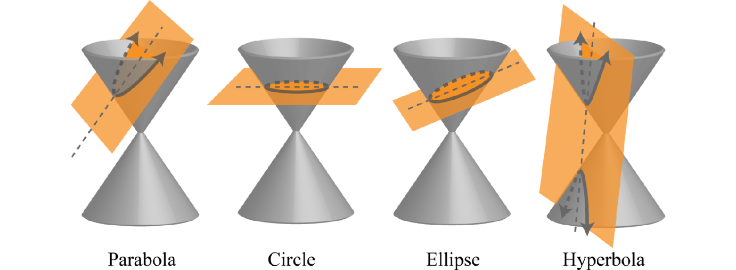
\includegraphics[scale = 0.5]{ConicSection.png}\\
(Taken from Geogebra)
\end{center}
Except parabola, others can be expressed in terms of quadratic forms. What distinguishes them is the discriminant of the quadratic equation.
\begin{proper}
Ellipses, circles, and hyperbola centered at the origin have the form of
\begin{align*}
ax^2 + bxy + cy^2 = h
\end{align*}
where $a$, $b$, $c$ and $h$ are all constants. They can be classified by the discriminant $\Delta = b^2 - 4ac$. The discriminant is positive if the graph is a hyperbola. It is negative if the graph is an ellipse (additionally $b = 0$ and $a = c$ with a circle). However, there are chances that there are no real curves regardless of the value of discriminant. They can be written as $\vec{x}^TA\vec{x} = h$, where
\begin{align*}
A &= 
\begin{bmatrix}
a & \frac{1}{2}b \\
\frac{1}{2}b & c
\end{bmatrix}
\end{align*}
Notice that the determinant $\det(A)$ is $-\frac{1}{4}$ of the discriminant.
\end{proper}
The statement above does not mention what happens when the discriminant is zero. In fact it is due to the removal of linear terms in the quadratic forms. Quadratic equations, in the most general sense, have the form of $ax^2 + bxy + cy^2 + mx + ny = h$, with $m$ and $n$ are constants as well. A zero discriminant actually represents parabola, but the lack of linear terms in quadratic terms reduces the parabola to straight lines. Of course we can include the linear terms to encompass the parabola as well, but to make our discussion below simpler, we will stick to the quadratic form expression and only talk about the central conics.\\
Short Exercise: Identify the types of curve generated by $x^2 - xy + 2y^2 = 3$ and $x^2 + xy - y^2 = 1$.
\begin{center}
\begin{tikzpicture}
\draw[thick, ->] (-3,0) -- (3,0) node[right]{$x$};
\draw[thick, ->] (0,-3) -- (0,3) node[above]{$y$};
\draw[Green,rotate=30] plot[domain=-0.8:1] ({2*cosh(\x)},{1.5*sinh(\x)});
\draw[Green,rotate=30] plot[domain=-1:0.8] ({-2*cosh(\x)},{1.5*sinh(\x)});
\draw[red,rotate=30] plot[domain=-3:3] ({\x},{0});
\draw[blue,rotate=-60] plot[domain=-3:3] ({\x},{0});
\end{tikzpicture}
\begin{tikzpicture}
\draw[thick, ->] (-3,0) -- (3,0) node[right]{$x$};
\draw[thick, ->] (0,-3) -- (0,3) node[above]{$y$};
\draw[Green, rotate=-30] (0,0) ellipse (2.5 and 1.5);
\draw[red,rotate=-30] plot[domain=-3:3] ({\x},{0});
\draw[blue,rotate=60] plot[domain=-3:3] ({\x},{0});
\end{tikzpicture} \\
Left: A hyperbola ($\frac{11}{144}x^2 + \frac{25}{24\sqrt{2}}xy - \frac{13}{48}y^2 = 1$), Right: An ellipse ($\frac{52}{225}x^2 + \frac{32}{75\sqrt{3}}xy + \frac{28}{75}y^2 = 1$). Both of them are rotated in the sense that their major axis (red) and minor axis (blue) are not aligned and made a angle of 30 degrees with the $x$ and $y$ axes. Major axis always passes through the vertices, with the minor axis perpendicular to it.
\end{center}

The last properties actually has another interpretation in terms of matrix. But before that we need to introduce some new terminologies.
\begin{defn}
For any symmetric matrix $A$, the quadratic form $\vec{x}^T A\vec{x}$ is called
\begin{enumerate}[label=(\alph*)]
\item positive definite, if for any $\vec{x} \neq \vec{0}$, $\vec{x}^T A\vec{x} > 0$ (positive semi-definite if $\vec{x}^T A\vec{x} \geq 0$), 
\item negative definite, if for any $\vec{x} \neq \vec{0}$, $\vec{x}^T A\vec{x} < 0$ (negative semi-definite if $\vec{x}^T A\vec{x} \leq 0$), 
\item indefinite if $\vec{x}^T A\vec{x}$ can take both positive and negative values,
\end{enumerate}
\end{defn}
\begin{thm}
The quadratic form $\vec{x}^T A\vec{x}$ is
\begin{enumerate}[label=(\alph*)]
\item positive definite, if and only if all eigenvalues of $A$ are positive (positive semi-definite if and only if all eigenvalues of $A$ are non-negative), 
\item negative definite, if and only if all eigenvalues of $A$ are negative (negative semi-definite if and only if all eigenvalues of $A$ are non-positive), 
\item indefinite when there are both positive and negative eigenvalues for $A$.
\end{enumerate}
\end{thm}
Now we are ready to extend our results and see what the quadratic equation $\vec{x}^TA\vec{x} = h$ can give.
\begin{thm}
Given $\vec{x}^TA\vec{x} = h$, where $h$ is chosen to be $1$ for scaling, then it represents
\begin{enumerate}[label=(\alph*)]
\item an ellipse if $A$ is positive definite,
\item a hyperbola if $A$ is indefinite,
\item no real graph if $A$ is negative definite.
\end{enumerate}
\end{thm}
For example, the quadratic equation $\vec{x}^TA\vec{x} = 1$, where
\begin{align*}
A &=
\begin{bmatrix}
1 & -2 \\
-2 & 3
\end{bmatrix}
\end{align*}
is equivalent to $x^2 - 4xy + 3y^2 = 1$. $A$ has an eigenvalue of $\lambda = 2 \pm \sqrt{5}$. As $\lambda_+ = 2 + \sqrt{5} > 0$ and $\lambda_- = 2 - \sqrt{5} < 0$, $A$ is indefinite and the curves are a pair of hyperbola.\\
\\
The figure in the last page shows that hyperbola and ellipses can be rotated. The effect on the resulted quadratic equation is to produce cross-product terms ($xy$ in two-dimensional cases), which can be eliminated by a rotation to restore the curves so that the major and minor axes are oriented along the $x$ and $y$ axes. If the graphs start with tilted by an angle of $\theta$, we can make a rotation by the same angle $\theta$ but in an opposite sense to recover the standard position. It is equivalent to rotate the coordinate system by an angle of $\theta$ in the same sense of the initial tilting. Section \ref{orthogeometricsub} can be referenced.

\begin{exmp}
Rotate the quadratic equation $x^2 - xy + y^2 = 1$ so that the major axis lies along the $x$-axis. \\
\\
First, we cast the equation into quadratic form $\vec{x}^T A\vec{x}$, with
\begin{align*}
A &=
\begin{bmatrix}
1 & -\frac{1}{2} \\
-\frac{1}{2} & 1
\end{bmatrix}
\end{align*}
We first find the eigenvalues of $A$, the characteristic equation is
\begin{align*}
(1-\lambda)^2 - (-\frac{1}{2})^2 &= 0 \\
\lambda^2 - 2\lambda + \frac{3}{4} &= 0 \\
\lambda &= \frac{1}{2} \text{ or } \frac{3}{2}
\end{align*}
So by the theorem above, $A$ is positive definite and it is an ellipse. We will see very soon the smaller eigenvalue actually corresponds to the major axis. Now we consider an orthogonal matrix $P$ to perform a rotation on the coordinate system, with the old coordinates related to the new coordinates by $\vec{x} = P\vec{x'}$. So the quadratic form is transformed to
\begin{align*}
(P\vec{x'})^T A (P\vec{x'}) &= \vec{x'}^T (P^T AP) \vec{x'}
\end{align*}
We immediately identify $P^T AP$ as a rotation of the coordinate system for the matrix $A$, as noted by the remark at the end of section \ref{orthogonaldiagreal}. The same section tells us that we can deal with the cross product terms by orthogonal diagonalization, which removes the off-diagonal entries in $A$. The normalized eigenvectors are
\begin{align*}
&\vec{v_\lambda} = \begin{bmatrix}
\frac{1}{\sqrt{2}} \\
\frac{1}{\sqrt{2}}
\end{bmatrix}
\text{ for } \lambda = \frac{1}{2}
& \begin{bmatrix}
-\frac{1}{\sqrt{2}} \\
\frac{1}{\sqrt{2}}
\end{bmatrix}
\text{ for } \lambda = \frac{3}{2}
\end{align*}
Hence we can set 
\begin{align*}
P =
\begin{bmatrix}
\frac{1}{\sqrt{2}} & -\frac{1}{\sqrt{2}} \\
\frac{1}{\sqrt{2}} & \frac{1}{\sqrt{2}}
\end{bmatrix}
\end{align*}
So that
\begin{align*}
P^T AP = 
\begin{bmatrix}
\frac{1}{\sqrt{2}} & \frac{1}{\sqrt{2}} \\
-\frac{1}{\sqrt{2}} & \frac{1}{\sqrt{2}}
\end{bmatrix}
\begin{bmatrix}
1 & -\frac{1}{2} \\
-\frac{1}{2} & 1
\end{bmatrix}
\begin{bmatrix}
\frac{1}{\sqrt{2}} & -\frac{1}{\sqrt{2}} \\
\frac{1}{\sqrt{2}} & \frac{1}{\sqrt{2}}
\end{bmatrix}
=
\begin{bmatrix}
\frac{1}{2} & 0\\
0 & \frac{3}{2}
\end{bmatrix}
= D
\end{align*}
The smaller eigenvalue is located at the first row/column, meaning now the major axis matches the new $x$-axis. The new equation is seen to be $\vec{x'}^T D\vec{x}$, or $\frac{1}{2}(x')^2 + \frac{3}{2}(y')^2 = 1$. Below are the diagrams before and after the rotation.

\begin{center}
\begin{tikzpicture}
\draw[thick, ->] (-3,0) -- (3,0) node[right](vecu){$x$};
\draw[thick, ->] (0,-3) -- (0,3) node[above]{$y$};
\draw[Green, thick, rotate=45] (0,0) ellipse ({1.2*sqrt(2)} and {1.2*sqrt(2/3)});
\draw[red, ->] (0,0) -- (2,2) node[above right](vecv){$x'$, Major axis, $\lambda = 1/2$};
\draw[blue, ->] (0,0) -- (-1,1) node[above left]{$y'$, Minor axis, $\lambda = 3/2$};
\node[Green] at (2,-2) {$x^2 - xy + y^2 = 1$};
\pic[draw, ->, "$45^\circ$", angle eccentricity=1.75] {angle = vecu--0--vecv};
\end{tikzpicture}
(Before rotation) \\
\begin{tikzpicture}
\draw[red, thick, ->] (-3,0) -- (3,0) node[right](vecu){$x'$};
\draw[blue, thick, ->] (0,-3) -- (0,3) node[above]{$y'$};
\draw[Green, thick, rotate=0] (0,0) ellipse ({1.2*sqrt(2)} and {1.2*sqrt(2/3)});
\node[Green] at (2,-2) {$\frac{1}{2}(x')^2 + \frac{3}{2}(y')^2 = 1$};
\end{tikzpicture} 
(After rotation)
\end{center}
The degree of tilting can be found to be exactly $\pi/4 = 45^{\circ}$, by comparing the general two-dimensional rotation matrix
\begin{align*}
\begin{bmatrix}
\cos \theta & -\sin \theta \\
\sin \theta & \cos \theta
\end{bmatrix}
\end{align*}
against $P$. $\cos \theta = \frac{1}{\sqrt{2}}$ and $\sin \theta = \frac{1}{\sqrt{2}}$ implies that $\tan \theta = 1$, and $\theta = \pi/4$. The possibility of eliminating the cross-product terms in quadratic forms is formally known as the Principal Axes Theorem.
\end{exmp}
\begin{thm}
For a quadratic form $\vec{x}^TA\vec{x}$, where $A$ is symmetric, we can always make an orthogonal change of variable $\vec{x'} = P^T\vec{x}$ or $\vec{x} = P\vec{x'}$ such that it turns into $\vec{x'}^TD\vec{x'} = \lambda_1 x_1'^2 + \lambda_2 x_2'^2 + \cdots$ which contains no cross-product terms. $P$ is formed by the set of orthonormal column eigenvectors of $A$ and $D$ is a diagonal matrix with entries being the eigenvalues of $A$.
\end{thm}
In general, for a two-dimensional quadratic form
\begin{align*}
\begin{bmatrix}
a & b \\
b & c
\end{bmatrix}
\end{align*}
It can undergo a rotation of the coordinate system by an angle $\theta$ such that
\begin{align*}
\begin{bmatrix}
\cos \theta & \sin \theta \\
-\sin \theta & \cos \theta
\end{bmatrix}
\begin{bmatrix}
a & b \\
b & c
\end{bmatrix}
\begin{bmatrix}
\cos \theta & -\sin \theta \\
\sin \theta & \cos \theta
\end{bmatrix}
=
\begin{bmatrix}
* & 0\\
0 & *
\end{bmatrix}
\end{align*}
the off-diagonal elements become zero. The required $\theta$ is found by  expanding the left hand side and equating both sides, which gives
\begin{align*}
-\sin \theta (a \cos\theta + b\sin \theta) + \cos\theta (b \cos \theta + c\sin \theta) &= 0 \\
\frac{c-a}{2} \sin (2\theta) + b\cos(2\theta) &= 0 \\
\cot(2\theta) &= \frac{a-c}{2b}
\end{align*}
where we apply the familiar double angle formulas.

\section{Statistics with Quadratic Form}
\subsection{Variance}
\label{variancesec}
\subsubsection{Single Distribution}
One important measure in the world of Statistics is the variance of a distribution, or a time-series. Variance can be viewed as the spread of a distribution. Below is the definition of variance for a distribution made up by one single variable.
\begin{defn}
\label{variance}
For a distribution $X$, with $n$ data $x_1, x_2, x_3, \cdots, x_n$, its population variance is
\begin{align*}
\sigma^2 = \text{Var}(X) &= \frac{1}{n} ((x_1 - \mu)^2 + (x_2 - \mu)^2 + (x_3 - \mu)^2 + \cdots + (x_n - \mu)^2) \\
&= \frac{1}{n} \sum_{k=1}^n (x_k - \mu)^2
\end{align*}
where $\mu$ is the mean, or expected value of $X$, and is computed by
\begin{align*}
\mu = E(X) = \frac{1}{n} (x_1 + x_2 + x_3 + \cdots + x_n)
\end{align*}
\end{defn}
A simpler formula for computing the population variance is
\begin{align*}
\sigma^2 = E(X^2) - (E(X))^2 = E(X^2) - \mu^2
\end{align*}
For a finite sample, we may also want to use the sample variance $s^2$, which is the population variance multiplied by a factor of $\frac{n}{n-1}$. \\
As an example, given a dataset $X$, with $5$ data $\vec{x} = (1, 3, 6, 9, 11)^T$, then the mean is
\begin{align*}
\mu = \frac{1}{5}(1 + 3 + 6 + 9 + 11) = 6
\end{align*}
and the population variance is
\begin{align*}
\sigma^2 = \frac{1}{5}((1-6)^2 + (3-6)^2 + (6-6)^2 + (9-6)^2 + (11-6)^2) = 13.6
\end{align*}
We can also use the short-cut formula.
\begin{align*}
\sigma^2 &= E(X^2) - \mu^2 \\
&= \frac{1}{5} (1^2 + 3^2 + 6^2 + 9^2 + 11^2) - 6^2 \\
&= 49.6 - 36 \\
&= 13.6
\end{align*}
Short Exercise: Find the sample variance of $X$.\\
\\
The variance formula in Definition \ref{variance} can be written in quadratic form as follows.
\begin{proper}
Given a distribution $X$, with $n$ data $\vec{x} = (x_1, x_2, x_3, \cdots, x_n)^T$, and a mean of $\mu$, the population variance can be written as
\begin{align*}
\frac{1}{n} (\vec{x'}\cdot\vec{x'}) = \frac{1}{n} \textbf{x}'^T \textbf{x}'
\end{align*}
where $\textbf{x}' = \vec{x'} = \vec{x} - \mu$ is the centered distribution with the mean $\mu$ removed. It can also be expressed as the quadratic form $\vec{x'}^T B'\vec{x'}$, where
\begin{align*}
B' &=
\begin{bmatrix}
\frac{1}{n} & 0 & 0 & \cdots \\
0 & \frac{1}{n} & 0 & \\
0 & 0 & \frac{1}{n} & \\
\vdots & & & \ddots
\end{bmatrix}
\end{align*}
is a diagonal matrix. The sample variance simply has all diagonal entries $\frac{1}{n}$ replaced by $\frac{1}{n-1}$.
\end{proper}
If we want to express the variance without involving $\mu$, then we can notice that
\begin{align*}
x'_1 &= x_1 - \frac{1}{n}(x_1 + x_2 + \cdots + x_n) = (1-\frac{1}{n})x_1 - \frac{1}{n} x_2 - \cdots - \frac{1}{n} x_n \\
x'_2 &= x_2 - \frac{1}{n}(x_1 + x_2 + \cdots + x_n) = -\frac{1}{n} x_1 + (1-\frac{1}{n}) x_2 - \cdots - \frac{1}{n} x_n \\
\cdots &= \cdots \\
x'_n &= x_n - \frac{1}{n}(x_1 + x_2 + \cdots + x_n) = -\frac{1}{n} x_1 - \frac{1}{n} x_2 - \cdots +(1-\frac{1}{n}) x_n 
\end{align*}
Hence
\begin{align*}
\vec{x'} = M\vec{x} = 
\begin{bmatrix}
1-\frac{1}{n} & -\frac{1}{n} & -\frac{1}{n} & \cdots \\
-\frac{1}{n} & 1-\frac{1}{n} & -\frac{1}{n} & \\
-\frac{1}{n} & -\frac{1}{n} & 1-\frac{1}{n} & \\
\vdots & & & \ddots
\end{bmatrix}
\vec{x}
\end{align*}
where $M$ is symmetric as well. Therefore, the desired expression is
\begin{align*}
\vec{x'}^T B'\vec{x'} &= (M\vec{x})^T B' (M\vec{x}) \\
&= \vec{x}^T (M^TB' M) \vec{x} = \vec{x}^T B \vec{x}
\end{align*}
where
\begin{align*}
B &= M^TB' M \\
&= 
\begin{bmatrix}
1-\frac{1}{n} & -\frac{1}{n} & -\frac{1}{n} & \cdots \\
-\frac{1}{n} & 1-\frac{1}{n} & -\frac{1}{n} & \\
-\frac{1}{n} & -\frac{1}{n} & 1-\frac{1}{n} & \\
\vdots & & & \ddots
\end{bmatrix}
\begin{bmatrix}
\frac{1}{n} & 0 & 0 & \cdots \\
0 & \frac{1}{n} & 0 & \\
0 & 0 & \frac{1}{n} & \\
\vdots & & & \ddots
\end{bmatrix}
\begin{bmatrix}
1-\frac{1}{n} & -\frac{1}{n} & -\frac{1}{n} & \cdots \\
-\frac{1}{n} & 1-\frac{1}{n} & -\frac{1}{n} & \\
-\frac{1}{n} & -\frac{1}{n} & 1-\frac{1}{n} & \\
\vdots & & & \ddots
\end{bmatrix} \\
&= \frac{1}{n}
\begin{bmatrix}
1-\frac{1}{n} & -\frac{1}{n} & -\frac{1}{n} & \cdots \\
-\frac{1}{n} & 1-\frac{1}{n} & -\frac{1}{n} & \\
-\frac{1}{n} & -\frac{1}{n} & 1-\frac{1}{n} & \\
\vdots & & & \ddots
\end{bmatrix} 
\begin{bmatrix}
1-\frac{1}{n} & -\frac{1}{n} & -\frac{1}{n} & \cdots \\
-\frac{1}{n} & 1-\frac{1}{n} & -\frac{1}{n} & \\
-\frac{1}{n} & -\frac{1}{n} & 1-\frac{1}{n} & \\
\vdots & & & \ddots
\end{bmatrix} \\
&= 
\frac{1}{n}
\begin{bmatrix}
1-\frac{1}{n} & -\frac{1}{n} & -\frac{1}{n} & \cdots \\
-\frac{1}{n} & 1-\frac{1}{n} & -\frac{1}{n} & \\
-\frac{1}{n} & -\frac{1}{n} & 1-\frac{1}{n} & \\
\vdots & & & \ddots
\end{bmatrix} =
\begin{bmatrix}
\frac{n-1}{n^2} & -\frac{1}{n^2} & -\frac{1}{n^2} & \cdots \\
 -\frac{1}{n^2} & \frac{n-1}{n^2} & -\frac{1}{n^2} & \\
 -\frac{1}{n^2} & -\frac{1}{n^2} & \frac{n-1}{n^2} & \\
\vdots & & & \ddots
\end{bmatrix}
\end{align*}
The readers are invited to verify that $M^TM = M^2 = M$ as shown in the calculation above. To obtain the sample variance, multiply the whole expression by the factor $\frac{n}{n-1}$. Also, due to the nature of variance that it can never be negative, $B$ is positive semi-definite.\\
Short Exercise: Discuss under what situation the variance will be zero.

\subsubsection{Linear Combination of Multiple Distributions}
Sometimes we may need to consider the distribution of the sum of multiple variables. More generally, given any linear combination of multiple distributions, like $Z = c_1X^{(1)} + c_2X^{(2)} + \cdots + c_nX^{(n)}$, we may want to know about its mean and variance. The mean will be simply $\mu_Z = c_1\mu_1 + c_2\mu_2 + \cdots + c_n\mu_n$, where $\mu_j$ is the mean of $X^{(j)}$. The variance $\text{Var}(Z)$ is a bit more complicated. First, we need to introduce the concept of covariance between any two distributions, which is
\begin{defn}
\label{covariance}
For two distributions $X$ and $Y$, each with $n$ pairs of members, their population covariance is
\begin{align*}
\text{Cov}(X,Y) &= \frac{1}{n}((x_1-\mu_x)(y_1-\mu_y) + (x_2-\mu_x)(y_2-\mu_y)) + \cdots + (x_n-\mu_x)(y_n-\mu_y)) \\
&= \frac{1}{n}\sum_{k=1}^{n} (x_k-\mu_x)(y_k-\mu_y)
\end{align*}
where $\mu_x$ and $\mu_y$ are the population means of $X$ and $Y$ respectively. The order does not matter, as $\text{Cov}(X,Y) = \text{Cov}(Y,X)$. If $\vec{x'}$ and $\vec{y'}$ are the centered data with their mean subtracted away, then it can be denoted by the vector notation as
\begin{align*}
\frac{1}{n} \vec{x'} \cdot \vec{y'} = \frac{1}{n} \textbf{x}'^T \textbf{y}'
\end{align*}
For sample covariance, it is
\begin{align*}
q_{xy} = \frac{1}{n-1} \sum_{k=1}^{n} (x_k-\bar{x})(y_k-\bar{y})
\end{align*}
where $\bar{x}$ and $\bar{y}$ are the sample means of $X$ and $Y$ which happen to have the same values as $\mu_x$ and $\mu_y$.
\end{defn}
There are short-cut formula similar as that for variance. The population covariance can be computed as
\begin{align*}
\text{Cov}(X,Y) &= E(XY) - E(X)E(Y)    
\end{align*}
The sample covariance has an additional factor of $\frac{n}{n-1}$. Also, a direct comparison reveals that $\text{Cov}(X,X) = \text{Var}(X)$ for any distribution $X$.

\begin{exmp}
Two time-series of zonal and meridional wind speed $U$ and $V$, have measurements as shown in the table below.
\begin{center}
\begin{tabular}{|c|c|c|}
\hline
(in \si{\m \per \s}) & $U$ & $V$\\
\hline
1st Measurement & 4 & -3 \\
\hline
2nd Measurement & 3 & -1 \\
\hline
3nd Measurement & 3 & -2 \\
\hline
4th Measurement & 2 & -1 \\
\hline
\end{tabular}
\end{center}
Find the covariance of $U$ and $V$.\\
It is not hard to get $\mu_u = 3$ and $\mu_v = -\frac{7}{4}$. From the definition, we have
\begin{align*}
\text{Cov}(U,V) &= \frac{1}{4} [(4-3)((-3)-(-1.75))+(3-3)((-1)-(-1.75)) \\
&\quad+(3-3)((-2)-(-1.75))+(2-3)((-1)-(-1.75))] \\
&= \SI{-0.5}{\square\m \per \square\s}
\end{align*}
Alternatively, the short-cut formula gives
\begin{align*}
\text{Cov}(U,V) &= E(UV) - \mu_u \mu_v \\
&= \frac{1}{4}((4)(-3) + (3)(-1) + (3)(-2) + (2)(-1)) - (3)(-\frac{7}{4}) \\
&= (-5.75) - (-5.25) = \SI{-0.5}{\square\m \per \square\s}
\end{align*}
\end{exmp}
Remember we use the formula for population covariance, and we have to scale by an appropriate factor when computing the sample covariance. From the example, we can make two observations. First, if $X$ and $Y$ both have the same unit $a$, then the unit of their covariance, or the variance for each of them individually, have the unit of $a^2$. Also, covariance can take negative values, which is different from variance which is always non-negative.\\
\\
Another useful measure related to variance and covariance is correlation. For two distribution $X$ and $Y$, the correlation is defined by the following formula.
\begin{defn}
The correlation of two distributions $X$ and $Y$ is
\begin{align*}
\rho_{xy} &= \frac{\text{Cov}(X,Y)}{\sqrt{\text{Var}(X) \text{Var}(Y)}} \\
&= \frac{\text{Cov}(X,Y)}{\sqrt{\text{Cov}(X,X) \text{Cov}(Y,Y)}}
\end{align*}
\end{defn}
Moreover,
\begin{defn}
The correlation between any two distributions $X$ and $Y$ falls in the range of $-1$ and $1$, i.e. $-1 \leq \rho_{xy} \leq 1$.
\paragraph{Proof} We can rewrite the correlation using vector notation for covariance, which gives
\begin{align*}
\rho_{xy} &= \frac{(\vec{x'} \cdot \vec{y'})}{\sqrt{(\vec{x'}\cdot\vec{x'})(\vec{y'}\cdot\vec{y'})}} \\
&= \frac{(\vec{x'} \cdot \vec{y'})}{\sqrt{{\norm{\vec{x'}}}\norm{\vec{y'}}}}
\end{align*}
where $\vec{x'}$ and $\vec{y'}$ are centered by removing the mean from the original distributions. By comparing to Cauchy-Schwarz Inequality proved in Theorem \ref{CauchySch}, we promptly know that $\abs{\rho_{xy}} \leq 1$.
\end{defn}
Correlation between two distributions $X$ and $Y$ indicates how their data varies together in a linear fashion. If the correlation is positive, then $X$ and $Y$ will increase or decrease together. However, if the correlation is negative, then when one of them increases, one of them will decrease, and vice versa. Higher the correlation, stronger the relationship. If the correlation is close to zero, it means that there are no clear linear relationship between them, however this does not exclude the possibility of having other relationship, e.g. exponential.
\begin{center}
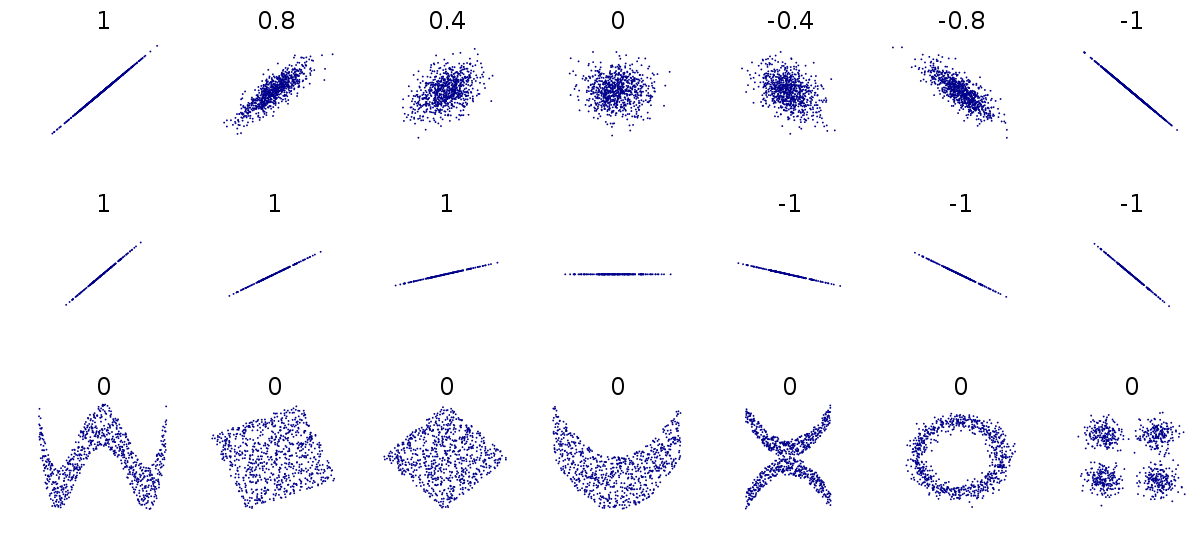
\includegraphics[scale = 0.3]{1200px-Correlation_examples2.svg.png}\\
(Taken from Wikipedia)
\end{center}
In the last example, $\text{Cov}(U,V) = \SI{-0.5}{\square\m \per \square\s}$, $\text{Var}(U) = \SI{0.5}{\square\m \per \square\s}$,\\
$\text{Var}(V) = \SI{0.6875}{\square\m \per \square\s}$, and $\rho_{uv} = \frac{0.5}{\sqrt{(0.5)(0.6875)}} \approx -0.8528$. We use the population variance and covariance for the computation, but they can be replaced by the sample counterparts at once. It may be tempting to claim that a strong negative relationship exists in this case. However, we note that the sample size here is a bit small for this result to be meaningful. Also, correlation is always dimensionless.\\
\\
We are now prepared to derive the variance formula for linear combinations of multiple variables.
\begin{proper}
\label{variancemul}
For a distribution made up of multiple variables, in the form of $Z = c_1X^{(1)} + c_2X^{(2)} + \cdots + c_nX^{(n)}$, with $\vec{c} = (c_1, c_2, \cdots, c_n)^T$ are all constants, the population variance $\text{Var}(Z)$ can be expressed as a quadratic form $\vec{c}^TQ\vec{c}$, where
\begin{align*}
Q &=
\begin{bmatrix}
\text{Cov}(X^{(1)}, X^{(1)}) & \text{Cov}(X^{(1)}, X^{(2)}) & \cdots & \text{Cov}(X^{(1)}, X^{(n)}) \\
\text{Cov}(X^{(2)}, X^{(1)}) & \text{Cov}(X^{(2)}, X^{(2)}) & \cdots & \text{Cov}(X^{(2)}, X^{(n)}) \\
\vdots & \vdots &  & \vdots \\
\text{Cov}(X^{(n)}, X^{(1)}) & \text{Cov}(X^{(n)}, X^{(2)}) & \cdots & \text{Cov}(X^{(n)}, X^{(n)}) \\
\end{bmatrix} \\
&=
\begin{bmatrix}
\text{Var}(X^{(1)}) & \text{Cov}(X^{(1)}, X^{(2)}) & \cdots & \text{Cov}(X^{(1)}, X^{(n)}) \\
\text{Cov}(X^{(2)}, X^{(1)}) & \text{Var}(X^{(2)}) & \cdots & \text{Cov}(X^{(2)}, X^{(n)}) \\
\vdots & \vdots &  & \vdots \\
\text{Cov}(X^{(n)}, X^{(1)}) & \text{Cov}(X^{(n)}, X^{(2)}) & \cdots & \text{Var}(X^{(n)}) \\
\end{bmatrix} 
\end{align*}
is the so-called covariance matrix. If $[X'] = [X'^{(1)}|X'^{(2)}|\cdots|X'^{(n)}]$ is consisted of the centered variables in columns, then $Q = \frac{1}{n}X'^TX$. To find the sample variance of $Z$, replace all $\text{Cov}(X^{(i)}, X^{(j)})$ by $q_{ij}$ in Definition \ref{covariance}.
\paragraph{Proof} To allow easier understanding, we will deal with the case of $n = 2$. However, the idea can be extended for other values of $n$. Starting from the expression in Definition \ref{variance}, we have
\begin{align*}
\text{Var}(Z) &= \frac{1}{n} \sum_{k=1}^n (z_k - \mu_z)^2 \\
&= \frac{1}{n} \sum_{k=1}^n ((c_1X^{(1)}_k + c_2X^{(2)}_k) - (c_1\mu_{x_1} + c_2\mu_{x_2}))^2 \\
&= \frac{1}{n} \sum_{k=1}^n (c_1(X^{(1)}_k - \mu_{x_1}) + c_2(X^{(2)}_k - \mu_{x_2}))^2 \\
&= \frac{1}{n} c_1^2 \sum_{k=1}^n (X^{(1)}_k - \mu_{x_1})^2 + \frac{1}{n} c_2^2 \sum_{k=1}^n (X^{(2)}_k - \mu_{x_2})^2 \\
&\quad+ \frac{2}{n} c_1c_2 \sum_{k=1}^n (X^{(1)}_k - \mu_{x_1}) (X^{(2)}_k - \mu_{x_2}) \\
&= c_1^2 \text{Cov}(X^{(1)}, X^{(1)}) + c_2^2 \text{Cov}(X^{(2)}, X^{(2)}) + 2c_1c_2 \text{Cov}(X^{(1)}, X^{(2)}) \\
&= c_1^2 \text{Cov}(X^{(1)}, X^{(1)}) + c_1c_2 \text{Cov}(X^{(1)}, X^{(2)}) \\
&\quad + c_2c_1 \text{Cov}(X^{(2)}, X^{(1)}) + c_2^2 \text{Cov}(X^{(2)}, X^{(2)}) \\
&= \sum_{i=1}^{n=2}\sum_{j=1}^{n=2} c_ic_j\text{Cov}(X^{(i)}, X^{(j)})
\end{align*}
where the terms are identified by Definition \ref{covariance}. By comparing to Definition \ref{quadform}, we realize the expression is simply
\begin{align*}
\vec{c}^TQ\vec{c} =
\begin{bmatrix}
c_1 & c_2
\end{bmatrix}
\begin{bmatrix}
\text{Cov}(X^{(1)}, X^{(1)}) & \text{Cov}(X^{(1)}, X^{(2)}) \\
\text{Cov}(X^{(2)}, X^{(1)}) & \text{Cov}(X^{(2)}, X^{(2)}) 
\end{bmatrix}
\begin{bmatrix}
c_1 \\
c_2
\end{bmatrix}
\end{align*}
for two variables situation.
\end{proper}

\begin{exmp}
From the previous wind speed example, if $W = 0.8U-0.6V$, find $\text{Var}(W)$.\\
\\
Earlier calculations show $\text{Var}(U) = \SI{0.5}{\square\m \per \square\s}$,
$\text{Var}(V) = \SI{0.6875}{\square\m \per \square\s}$, $\text{Cov}(U,V) = \text{Cov}(V,U) = \SI{-0.5}{\square\m \per \square\s}$. Plugging the values into the expression we just get, we have
\begin{align*}
\text{Var}(W) &=
\begin{bmatrix}
c_u & c_v
\end{bmatrix}
\begin{bmatrix}
\text{Var}(U) & \text{Cov}(U,V) \\
\text{Cov}(U,V) & \text{Var}(V)
\end{bmatrix}
\begin{bmatrix}
c_u \\
c_v
\end{bmatrix} \\
&=
\begin{bmatrix}
0.8 & -0.6
\end{bmatrix}
\begin{bmatrix}
0.5 & -0.5 \\
-0.5 & 0.6875
\end{bmatrix}
\begin{bmatrix}
0.8 \\
-0.6
\end{bmatrix} \\
&= \SI{1.0475}{\square\m \per \square\s}
\end{align*}
\end{exmp}

\subsection{Principal Component Analysis}
A common practice in Earth Science is to reduce the dimensions of a large set of data. Given a large number of variables, each with a substantial amount of measurements, we want to process them to extract and retain the most important features or signals. Principal Component Analysis, which also known as Empirical Orthogonal Function in atmospheric science, is the mainstream method to achieve this goal, by finding the pattern which maximizes the variance of the dataset. It will be explained slowly with some diagrams and helper theorems.\\
\\
Consider the simplest case with two variables, or time-series $X$ and $Y$ first. Assume they have $n$ pairs of entries, from $\vec{x_1}^T = (x_1, y_1)^T$ to $\vec{x_n}^T = (x_{n}, y_{n})^T$. We can compute the covariance matrix $Q$, introduced in the last section. Principal Component Analysis want to find a unit vector $\textbf{e}$, so that the variance of data along the direction indicated by $\textbf{e}$, which is $\textbf{e}^T Q \textbf{e}$ following from Properties \ref{variancemul}, is maximized.
\begin{center}
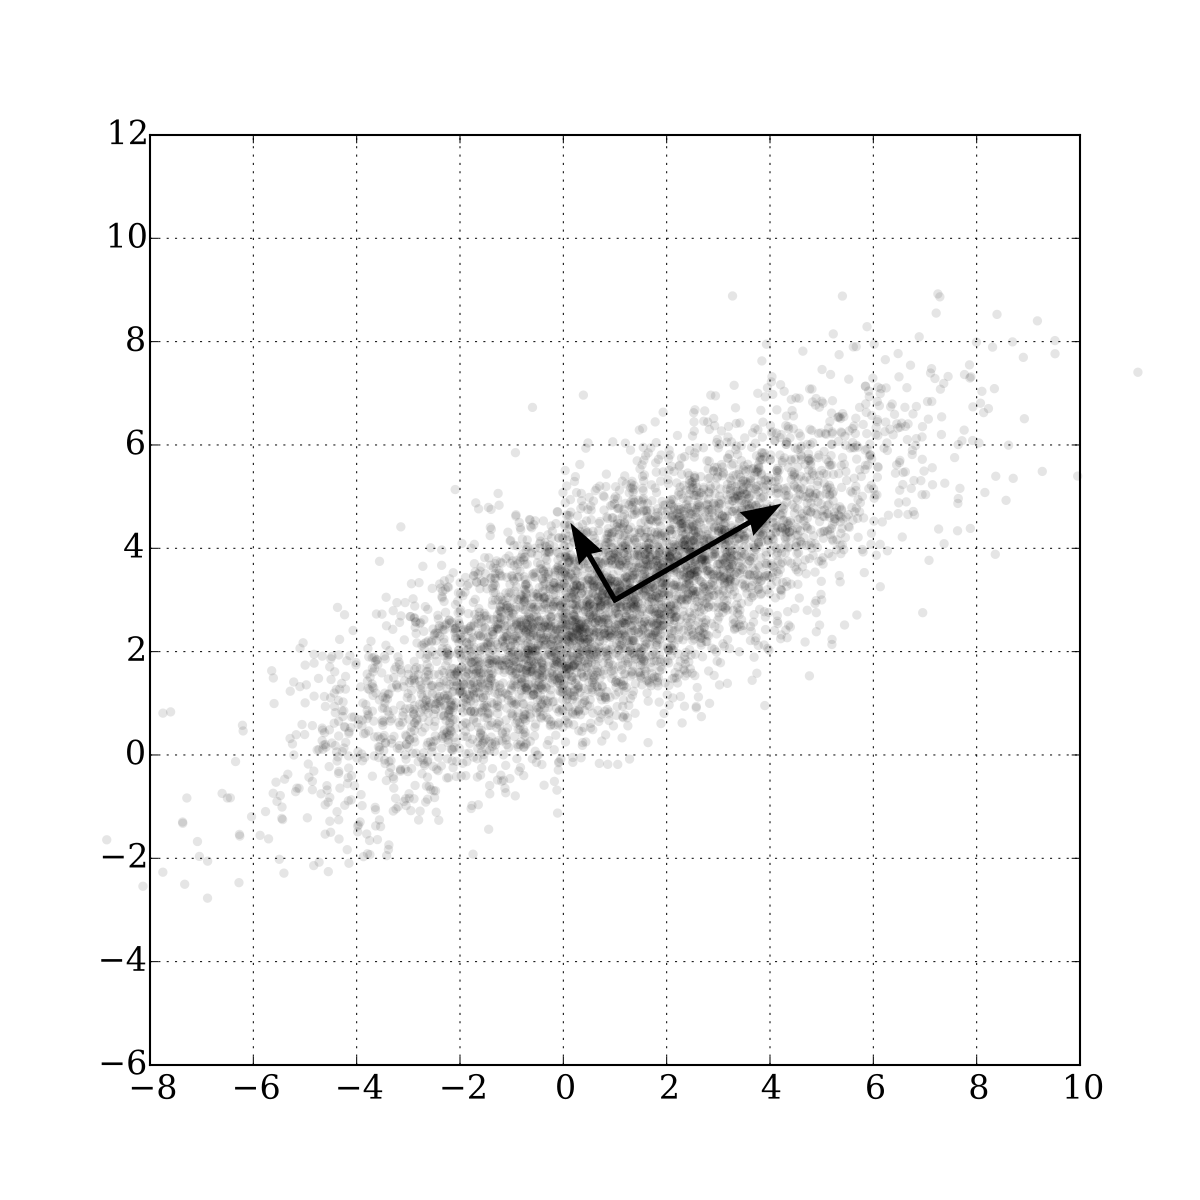
\includegraphics[scale = 0.15]{1200px-GaussianScatterPCA.svg.png}\\
Two principal axes found by Principal Component Analysis for a set of data. The longer vector represents the direction of largest variance. The data points can be seen to spread more along that direction. (Taken from Wikipedia)
\end{center}
Now the problem is to find, under what situation $\textbf{e}^T Q \textbf{e}$ will assume its largest value. Here, we introduce a famous technique, called the Lagrange Multiplier, which requires some knowledge in Calculus. As before, we will proceed with the 2 variables case for brevity.
\begin{thm}
\label{LagrangeMul}
To find the extremal values attained by a function $f(u,v,\cdots)$, under the constraint $g(u,v,\cdots) = 0$, we consider the expression
\begin{align*}
h(u,v,\cdots) = f(u,v,\cdots) - \lambda g(u,v,\cdots)
\end{align*}
where $\lambda$ is a constant to be determined by solving the system
\begin{align*}
\begin{cases}
\partial h/\partial u &= 0 \\
\partial h/\partial v &= 0 \\
\cdots &= 0
\end{cases}
\end{align*}
$\partial/\partial u$ and $\partial/\partial v$ means differentiating with $u$ and $v$ only while treating other variables as constants. The values of $u$ and $v$ to reach the extremums are also inferred from the set of equations above. 
\end{thm}
We are now going to find the value of $x'$ and $y'$ so that $\textbf{e}^T Q \textbf{e}$ obtains the maximum for $\textbf{e}^T = (x',y')$. The constraint is that $\textbf{e}$ is a unit vector as a direction, and hence by the method of Lagrange Multiplier outlined in Theorem \ref{LagrangeMul}, we have
\begin{align*}
g(x',y') = x'^2 + y'^2 - 1 = 0
\end{align*}
and with $f(x',y') = \textbf{e}^T Q \textbf{e}$
\begin{align*}
h(x',y') &= (\textbf{e}^T Q \textbf{e}) - \lambda(x'^2 + y'^2 - 1) \\
&= x'^2 \text{Cov}(X, X) + 2x'y' \text{Cov}(X, Y) + y'^2\text{Cov}(Y, Y) - \lambda(x'^2 + y'^2 - 1)
\end{align*}
according to Properties \ref{variancemul}. Carrying out the differentiation gives
\begin{align*}
\begin{cases}
\partial h/\partial x' &= 2x'\text{Cov}(X, X) + 2y'\text{Cov}(X, Y) - 2\lambda x' = 0 \\
\partial h/\partial y' &= 2x'\text{Cov}(X, Y) + 2y'\text{Cov}(Y, Y) - 2\lambda y' = 0
\end{cases}    
\end{align*}
This system can be immediately be recognised as
\begin{align*}
\begin{bmatrix}
\text{Cov}(X, X)-\lambda & \text{Cov}(X, Y) \\
\text{Cov}(Y, X) & \text{Cov}(Y, Y)-\lambda
\end{bmatrix}
\begin{bmatrix}
x' \\
y'
\end{bmatrix} &= 0\\
(Q-\lambda I)\vec{x'} &= 0
\end{align*}
which is an eigenvalue problem like those in Section \ref{eigensection}. Hence we conclude that $f(x',y') = \textbf{e}^T Q \textbf{e}$ attains its extremal values when $\textbf{e}^T = (x',y')^T$ is the unit eigenvector of $Q$. The corresponding magnitude of variance ${\textbf{e}^{(j)}}^T Q \textbf{e}^{(j)}$ for the $j$-th eigenvector is
\begin{align*}
{\textbf{e}^{(j)}}^T (Q \textbf{e}^{(j)}) &= {\textbf{e}^{(j)}}^T (\lambda^{(j)} \textbf{e}^{(j)}) \\
&= \lambda^{(j)} ({\textbf{e}^{(j)}}^T \textbf{e}^{(j)}) \\
&= \lambda^{(j)} (\hat{e}^{(j)} \cdot \hat{e}^{(j)}) \\
&= \lambda^{(j)} \norm{\hat{e}^{(j)}} \\
&= \lambda^{(j)}
\end{align*}
where we have used the facts that $Q \textbf{e}^{(j)} = \lambda^{(j)} \textbf{e}^{(j)}$ as per Definition \ref{eigen} and the length of a unit vector is $1$. This means that the variance along the direction of eigenvector is exactly the corresponding eigenvalue. To generalize for more variables, we have the following results.
\begin{thm}
For a covariance matrix $Q$ which happens to be symmetric, the variance $\textbf{e}^T Q \textbf{e}$ achieves its maximum value $\lambda_1$ along the direction $\textbf{e}^{(1)}$, which are the largest eigenvalue of $Q$ and the associated unit eigenvector. \\
Generally, if $Q$ has the orthonormal eigenvectors $\textbf{e}^{(1)}, \textbf{e}^{(2)}, \cdots, \textbf{e}^{(n)}$, arranged by the eigenvalues $\lambda_1 > \lambda_2 > \cdots > \lambda_n$, then the largest variance will be $\lambda_1$ when the direction is along $\textbf{e}^{(1)}$, the second largest will be  $\lambda_2$ for $\textbf{e}^{(2)}$ and so on, with the smallest variance being $\lambda_n$ for $\textbf{e}^{(n)}$. This set of linearly independent eigenvectors are called the Principal Directions in Principal Component Analysis.
\end{thm}
As a side note, any quadratic form $\hat{x}^TA\hat{x}$ will attain its maximum and minimum when $\hat{x}$ is the eigenvector that represents the largest and smallest eigenvalue, which are also the value $\hat{x}^TA\hat{x}$ takes when it happens. This is under the constraint that $\hat{x}$ is a unit vector, and has the name Constrained Extremum Theorem.\\
\\
Going back to the problem of Principal Component Analysis, for each Principal Directions $\textbf{e}^{(j)}$ and the variance $\lambda_{j}$, we can compute the ratio of explained variance, which is the fraction $\lambda_{j}$ over the total variance, that is the sum of eigenvalues for the covariance matrix. This number allows us to access how well the Principal Direction contributes to the total variance.\\
\\
With the set of orthonormal principal directions at hand, we can treat them as a coordinate basis and subsequently perform a rotation on the data as we have done earlier. Constructing a transition matrix made up of the Principal Directions $[\textbf{e}] = [\textbf{e}^{(1)}|\textbf{e}^{(2)}|\cdots|\textbf{e}^{(n)}]$, the new coordinates are $\vec{u} = [\textbf{e}]^T \vec{x}$ as suggested by Section \ref{orthogeometricsub}. $\vec{u_i}$ can be regarded to be the projection of $\vec{x_i}^T = (x_i, y_i)^T$ the $i$-th pair of data onto the principal directions and is called the Principal Components. By doing an orthogonal rotation on $Q$ by $[\textbf{e}]$, the resulted quantities $[\textbf{e}]^T Q[\textbf{e}]$ will be a diagonal matrix with non-trivial elements being the variances along the Principal Directions. \\
\\
Usually, at the start we will detrend the data and remove the mean from each variable, such that we use $x'_i = x_i - \bar{x}$ and $y'_i = y_i - \bar{y}$ to replace $x_i$ and $y_i$.

\begin{exmp}
The temperature data of two cities $M$ and $N$ are as follows.
\begin{center}
\begin{tabular}{|c|c|c|}
\hline
(in \si{\degree C}) & $M$ & $N$\\
\hline
1st Day & 22.1 & 22.3 \\
\hline
2nd Day & 21.8 & 21.6 \\
\hline
3nd Day & 20.9 & 21.2 \\
\hline
4th Day & 21.6 & 21.7 \\
\hline
5th Day & 23.4 & 23.2 \\
\hline 
6th Day & 24.7 & 24.1 \\
\hline 
7th Day & 22.0 & 23.9 \\
\hline 
8th Day & 22.1 & 22.4 \\
\hline 
\end{tabular}
\end{center}
Perform Principal Component Analysis and find the strongest Principal Direction, and extract the time-series related to this mode.\\
\\
After detrending, the data are
\begin{center}
\begin{tabular}{|c|c|c|}
\hline
(in \si{\degree C}) & $M'$ & $N'$\\
\hline
1st Day & -0.225 & -0.25 \\
\hline
2nd Day & -0.525 & -0.95 \\
\hline
3nd Day & -1.425 & -1.35 \\
\hline
4th Day & -0.725 & -0.85 \\
\hline
5th Day & 1.075 & 0.65 \\
\hline 
6th Day & 2.375 & 1.55 \\
\hline 
7th Day & -0.325 & 1.35 \\
\hline 
8th Day & -0.225 & -0.15 \\
\hline 
\end{tabular}
\end{center}
From Properties \ref{variancemul}, the sample covariance matrix is
\begin{align*}
Q = 
\frac{1}{8-1}
\begin{bmatrix}
\vec{m'}\cdot\vec{m'} & \vec{m'}\cdot\vec{n'} \\
\vec{n'}\cdot\vec{m'} & \vec{n'}\cdot\vec{n'} 
\end{bmatrix} =
\begin{bmatrix}
1.405 & 1.01 \\
1.01 & 1.1686
\end{bmatrix}
\end{align*}
The unit eigenvectors for $Q$ and thus the Principal Directions can be found to be $\textbf{e}^{(1)} = (0.747, -0.665)^T$ of larger variance $\lambda_1 = \SI{2.304}{\square {(\degree C)}}$, and $\textbf{e}^{(2)} = (0.665, 0.747)^T$ of smaller variance $\lambda_2 = \SI{0.270}{\square {(\degree C)}}$. The first principal component accounts for $2.304 / (2.304+0.270) \approx 89.5\%$ of the total variance.\\
\\
We can project every pair of data $\vec{x'}_i^T = (m'_i, n'_i)^T$ onto the principal directions by computing $\vec{u}_i = [\textbf{e}]^T\vec{x'}_i$, where $[\textbf{e}] = [\textbf{e}^{(1)}|\textbf{e}^{(2)}]$. The principal values are 
\begin{center}
\begin{tabular}{|c|c|c|c|c|c|c|c|c|}
\hline
(in \si{\degree C}) & D-1 & D-2 & D-3 & D-4 & D-5 & D-6 & D-7 & D-8 \\
\hline
$u^{(1)}$ & -0.334 & -1.024 & -1.962 & -1.107 & 1.235 & 2.805 & 0.655 & -0.268 \\
\hline
$u^{(2)}$ & -0.037 & -0.361 & -0.061 & -0.153 & -0.229 & -0.421 & 1.225 & 0.038 \\
\hline
\end{tabular}
\end{center}
In details, the principal components for the first day is computed by
\begin{align*}
\begin{bmatrix}
u_1^{(1)} \\
u_1^{(2)} 
\end{bmatrix}
=
\begin{bmatrix}
0.747 & 0.665 \\
-0.665 & 0.747
\end{bmatrix}
\begin{bmatrix}
-0.225 \\
-0.25
\end{bmatrix}
\end{align*}
The original dataset can be recovered by $\vec{x'}_i = [\textbf{e}]\vec{u'}_i$. If we want to extract the signals originated from the first Principal Directions, we can simply remove other column eigenvectors in $[\textbf{e}]$ and discard other principal values in $\vec{u'}_i$. The time-series reconstructed by the first mode is hence computed by $x'_i = \textbf{e}^{(1)}u_i^{(1)}$, which are
\begin{center}
\begin{tabular}{|c|c|c|c|c|c|c|c|c|}
\hline
(in \si{\degree C}) & D-1 & D-2 & D-3 & D-4 & D-5 & D-6 & D-7 & D-8 \\
\hline
$M'$ & -0.250 & -0.765 & -1.466 & -0.827 & 0.923 & 2.095 & 0.489 & -0.200 \\
\hline
$N'$ & -0.222 & -0.681 & -1.304 & -0.736 & 0.821 & 1.864 & 0.435 & -0.178 \\
\hline
\end{tabular}
\end{center}
\end{exmp}
\newpage
\begin{center}
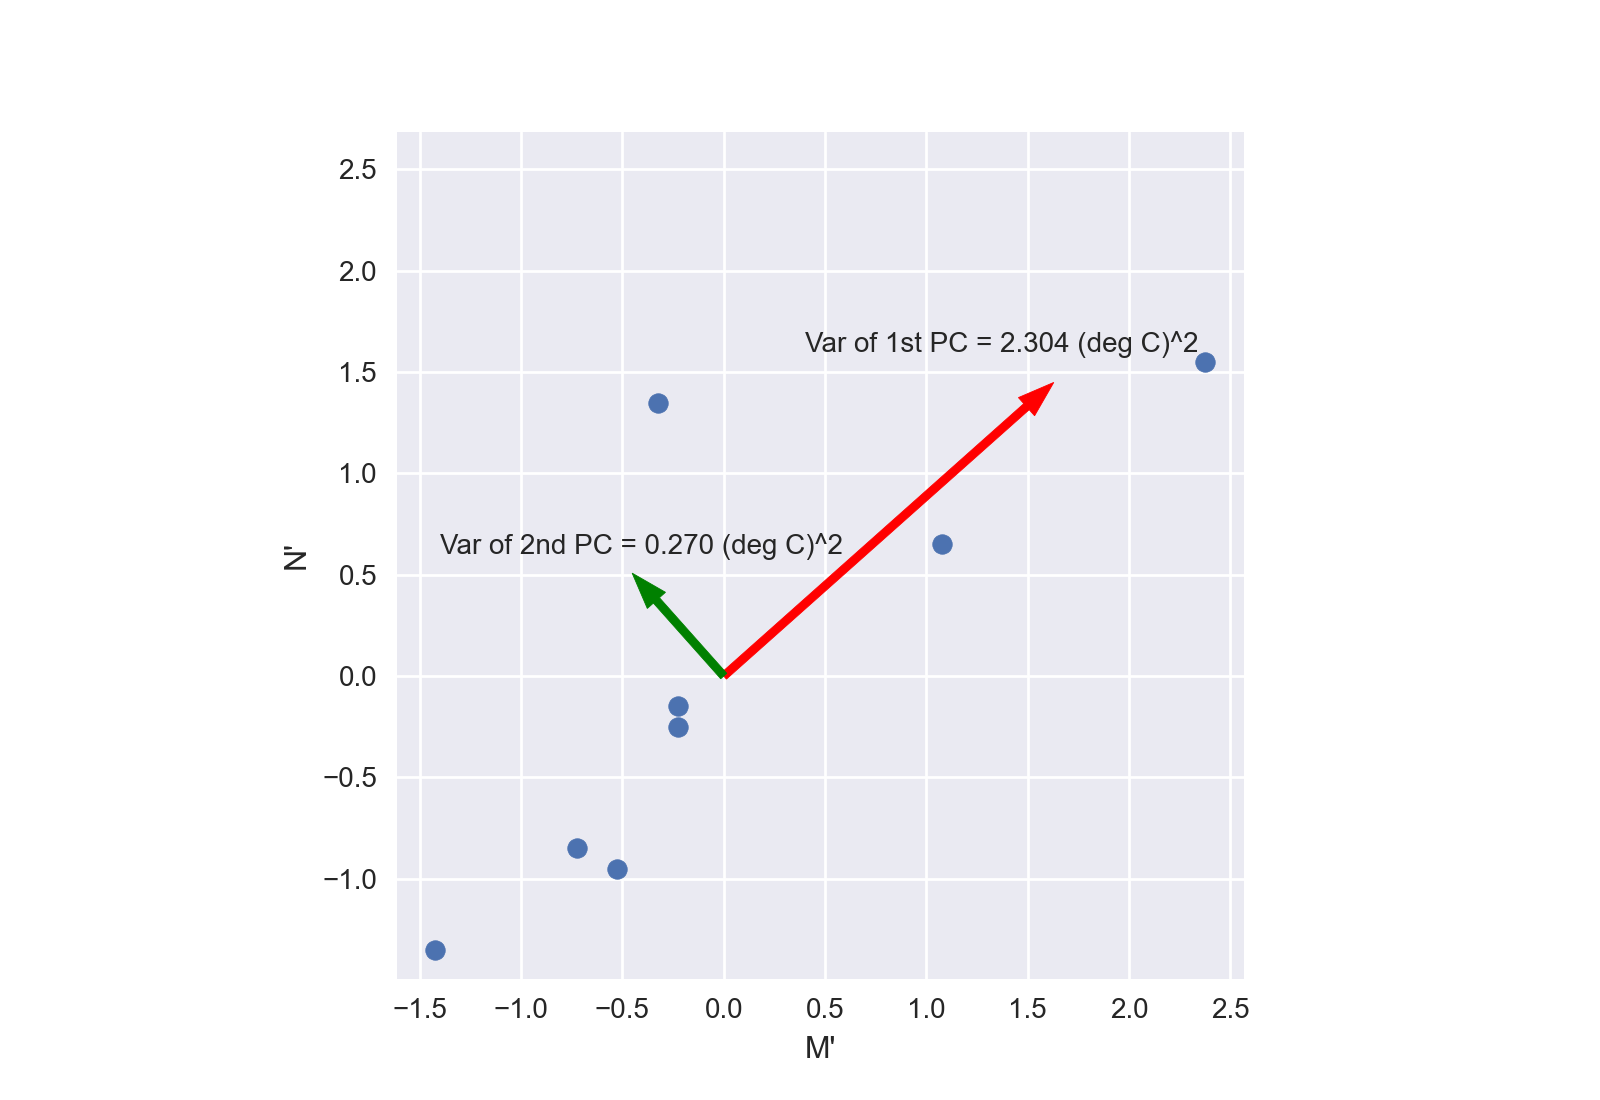
\includegraphics[scale = 0.6]{LAEOF.png}\\
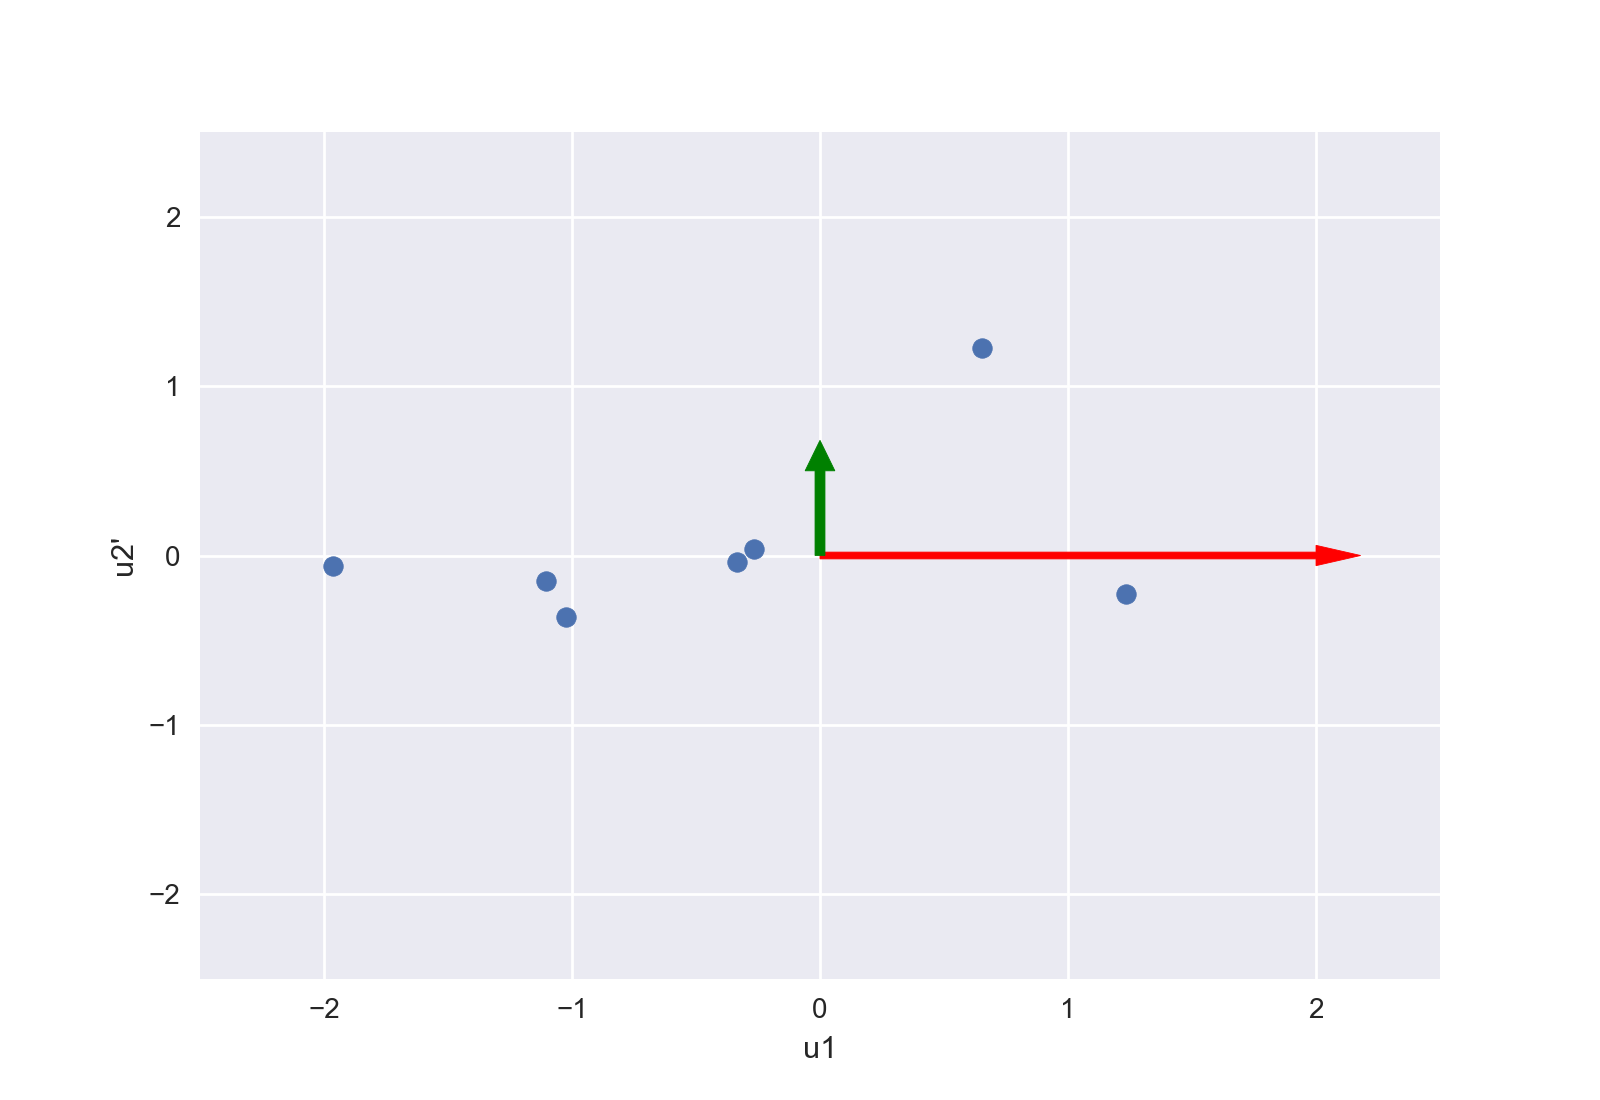
\includegraphics[scale = 0.6]{LAEOF2.png}\\
The data before and after rotation by the principal directions, with the one with larger/smaller variance shown as red/green.
\end{center}
\begin{center}
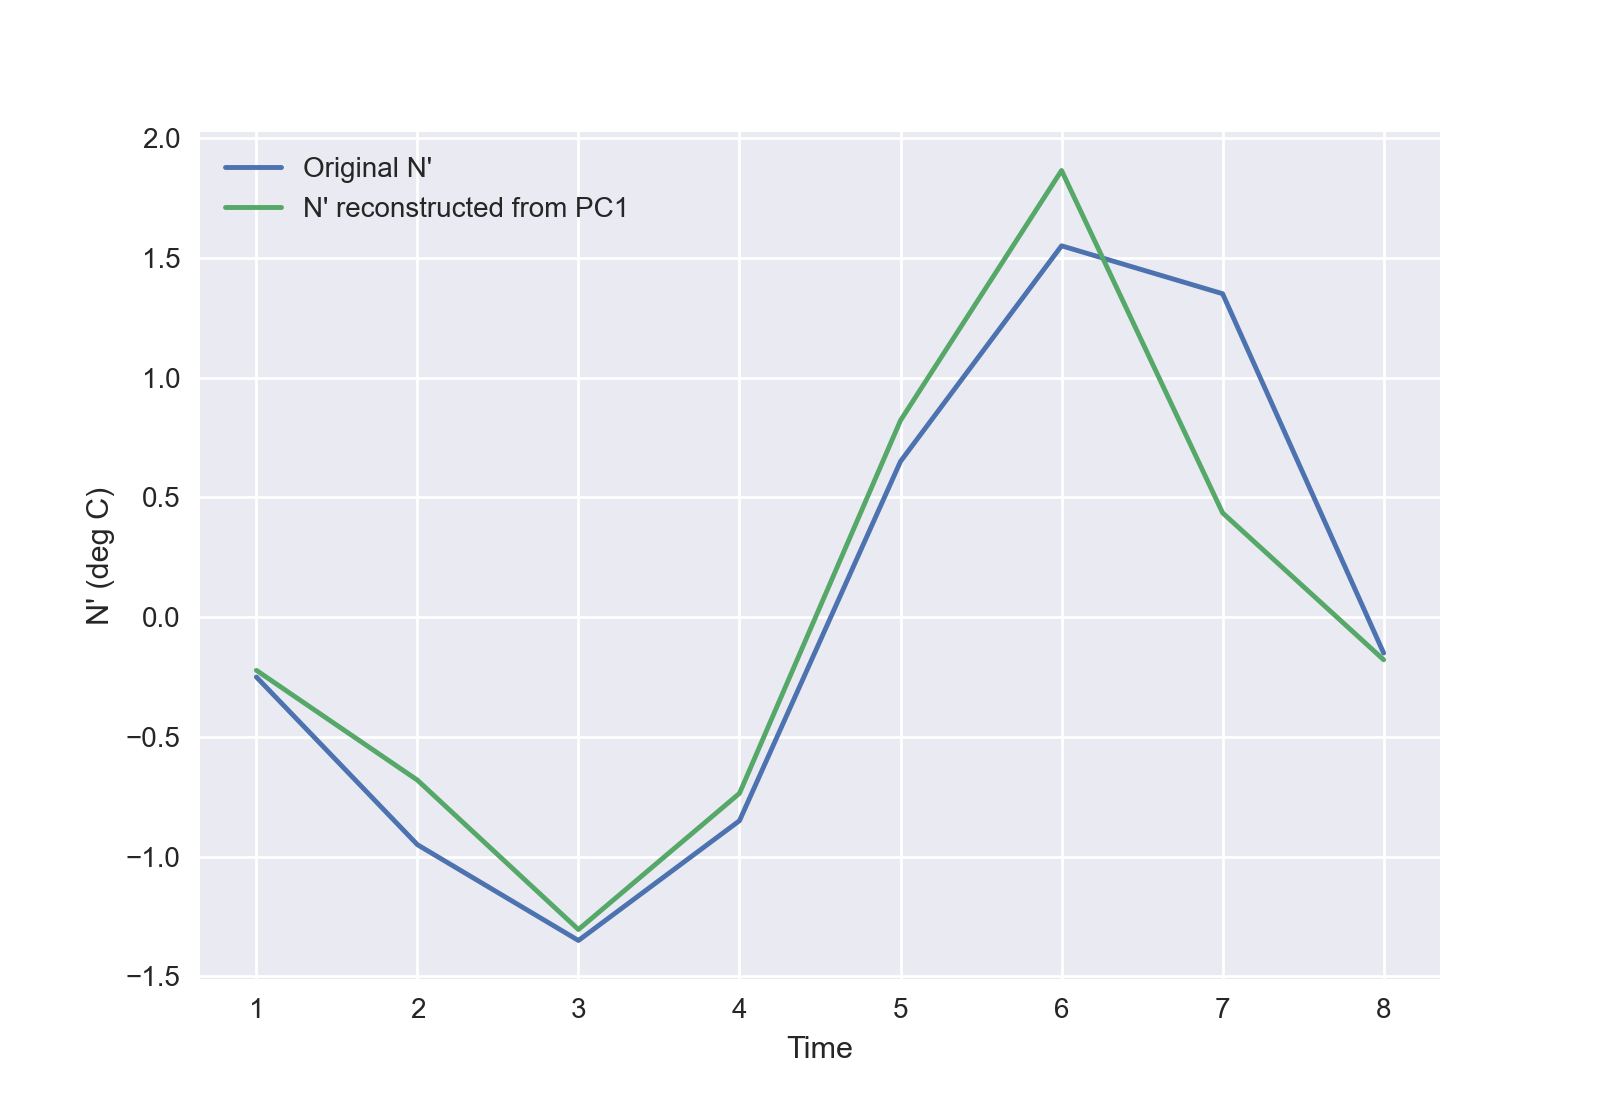
\includegraphics[scale = 0.6]{LAEOF3.png}\\
Comparison between the original anomaly and the first mode for $N'$.
\end{center}

\section{Exercise}

\begin{Exercise}
Identify the following conic sections and eliminate the cross-product terms by an appropriate rotation.
\begin{enumerate}[label=(\alph*)]
\item $x^2 + 5xy + 3y^2 = 1$,
\item $x^2 - xy + 2y^2 = 4$,
\item $x^2 + 2xy + y^2 = 1$, what is the curve generated? 
\end{enumerate}
\end{Exercise}

\begin{Exercise}
Find a new expression for the standard hyperbola $y^2 - x^2 = 1$ if a anti-clockwise rotation of $75$ degrees is done. What about a reflection along the $x$-axis?
\end{Exercise}

\begin{Exercise}
Three-dimensional quadrics can also be treated in a similar fashion to two-dimensional conic sections. Find the length of three axes for an ellipsoid $x^2 + y^2 + z^2 + 0.5xy - yz + 0.5xz = 1$ by doing an orthogonal coordinate transformation. What is the requirement for a three-dimensional quadratic form to represent an ellipsoid?
\end{Exercise}

\begin{Exercise}
Find the covariance matrix for three pressure time-series over $10$ days at cities $X$, $Y$, $Z$ (in hPa, relative to $1000$ hPa), which take the values
\begin{center}
\begin{tabular}{|c|c|c|}
\hline
$X$ & $Y$ & $Z$ \\
\hline
17 & 19 & 22 \\
\hline
18 & 16 & 25 \\
\hline
14 & 15 & 17 \\
\hline
19 & 21 & 23 \\
\hline
24 & 22 & 26 \\
\hline
21 & 20 & 23 \\
\hline 
28 & 26 & 29 \\
\hline
24 & 25 & 22 \\
\hline
20 & 21 & 27 \\
\hline
23 & 22 & 24 \\
\hline
\end{tabular}
\end{center}
Find the variance of $W = X - 0.5Y - 0.5Z$.
\end{Exercise}

\begin{Exercise}
Carry out Principal Component Analysis on the data set above. Find the Principal Directions and the ratio of explained variance for each of them. Reconstruct the data using the first Principal Direction with largest variance only.
\end{Exercise}


\chapter{Least-Square Approximation}

\section{Mathematical Ideas of Least-Square Approximation}

As discussed in Chapter \ref{chap:SolLinSys}, given a linear system $A\vec{x} = \vec{h}$, if the number of equations (rows) is greater than the number of unknowns (columns), then it is overdetermined. Generally, it would be inconsistent and no $\vec{x}$ can satisfy $A\vec{x} = \vec{h}$. However, a best-fit vector $\vec{x_f}$ can be found such that $A\vec{x_f} = \vec{h_f}$, the least-square error can be achieved in the sense that $\vec{h_f}$ has the closest distance to $\vec{h}$, i.e. the magnitude of the error vector $\vec{h}-\vec{h_f} = \vec{h}-A\vec{x_f}$ is minimized.\\
\\
It is stated that the desired vector $\vec{h_f} = A\vec{x_f}$ is the orthogonal projection of $\vec{h}$ onto the column space formed by column vectors in $A$. A simple description of column space can be found in Definition \ref{columnspace}. Intuitively, from a geometric viewpoint, $\vec{h_f} = A\vec{x_f}$ lies in the column space of $A$, and it would achieve the shortest distance to $\vec{h}$ if $\vec{h}-\vec{h_f}$ is orthogonal to column space of $A$. This also means that $A\vec{x} = \vec{h}$ has an exact solution if and only if $\vec{h}$ already lies in the column space of $A$.
\begin{center}
\begin{tikzpicture}
\filldraw[fill=Green!20]
(0,0,0) -- (4,0,0) -- (4,0,4) -- (0,0,4) -- cycle;
\draw[red, thick, ->] (1,0,1) -- (3,2,2) node[right]{$\vec{h}$};
\draw[blue, thick, ->] (1,0,1) -- (3,0,2) node[right]{$A\vec{x_f} = \vec{h_f}$};
\draw[gray, thick, dotted] (3,2,2) -- (3,0,2);
\node[Green] at (-2,0,1) {Column space of $A$};
\end{tikzpicture} \\
Geometric situation for the least-square approximation problem, when $A$ has 3 rows and 2 columns, $\vec{x_f}$ is a two-dimensional vector, while $\vec{h}$ and the orthogonal projection of $\vec{h}$ onto the column space of $A$, that is, $A\vec{x_f} = \vec{h_f}$ are three-dimensional vectors.
\end{center}

The remaining problem is to find either $\vec{h_f}$ or $\vec{x_f}$. Since the best-fit vector $\vec{h}-\vec{h_f}$ has to be orthogonal to all column vectors in $A$, $A^T(\vec{h}-\vec{h_f}) = \vec{0}$, as the dot products of rows in $A^T$ (columns in A) and $\vec{h}-\vec{h_f}$ evaluates to zero. Substitution and rearrangement gives
\begin{align*}
A^T(\vec{h}-\vec{h_f}) &= \vec{0} \\
A^T(\vec{h}-A\vec{x_f}) &= \vec{0} \\
A^T\vec{h} - A^TA\vec{x_f} &= \vec{0} \\
A^TA\vec{x_f} &= A^T\vec{h}
\end{align*}
This is called the normal equation due to the appearance of $A^TA$. Therefore,
\begin{align*}
\vec{x_f} &= (A^TA)^{-1}A^T\vec{h} \\  
\vec{h_f} &= A\vec{x_f} = A(A^TA)^{-1}A^T\vec{h}
\end{align*}
provided that the normal matrix $A^T A$ is invertible, which happens when $A$ consists of linearly independent column vectors.
\begin{thm}
\label{bestfit}
If $A$ is a $m \times n$ matrix with $m > n$ and all $n$ column vectors being linearly independent, then for the system $A\vec{x} = \vec{h}$, there exists a unique best-fit solution
\begin{align*}
\vec{x_f} &= (A^TA)^{-1}A^T\vec{h}    
\end{align*}
such that $\norm{\vec{h}-\vec{h_f}}^2 = \norm{\vec{h}-A\vec{x_f}}^2$ is minimized.
\end{thm}
However, if the column vectors in $A$ are not linearly independent, then the best-fit solution will not be unique. Rather, the normal equation will still be consistent, but there are infinitely many possible solutions, each having the same least-square error.\\
\\
Also, if we by chance have the QR decomposition of $A$, then
\begin{align*}
\vec{x_f} &= ((QR)^T(QR))^{-1}(QR)^T\vec{h} \\
&= (R^TQ^TQR)^{-1} (QR)^T\vec{h} \\
&= (R^TR)^{-1} R^TQ^T \vec{h} \\
&= R^{-1} (R^T){-1} R^TQ^T \vec{h} \\
&= R^{-1} Q^T\vec{h}
\end{align*}
$Q^TQ = I$ since $Q$ is orthogonal matrix as column vectors of $Q$ are orthonormal basis.

\section{Linear Regression}
\subsection{Linear Regression for One Predictor Variable}

Linear regression is a good example of least-square approximation. The simplest type of linear regression is fitting a straight line $y = \alpha + \beta x$ to $n$ pairs of observation, $(x_1, y_1), (x_2, y_2), \cdots, (x_n, y_n)$ such that the sum of squares error $\sum_{k=1}^n (y_k - (\alpha + \beta x_k))^2$ is minimized, optimizing the prediction of $y$ by $x$.

\begin{center}
\begin{tikzpicture}
\draw[thick, ->] (-1,0) -- (5,0) node[right]{$x$};
\draw[thick, ->] (0,-1) -- (0,5) node[above]{$y$};
\node[circle, inner sep=1pt, fill=blue] at (1,1.2) {};
\node at (0.8,1.6) {$(1,1.2)$};
\node[circle, inner sep=1pt, fill=blue] at (2,1.6) {};
\node at (2.2,1.2) {$(2,1.6)$};
\node[circle, inner sep=1pt, fill=blue] at (3,2.8) {};
\node at (3.2,2.4) {$(3,2.8)$};
\node[circle, inner sep=1pt, fill=blue] at (4,4.4) {};
\node at (3.8,4.8) {$(4,4.4)$};
\draw[thick, red] (-0.5,-0.74) -- (5,5.2) node[right]{$y = -0.2+1.08x$};
\node[below left]{$O$}; 
\draw[thick, Green] (1,1.2) -- (1,0.88);
\draw[thick, Green] (2,1.6) -- (2,1.96);
\draw[thick, Green] (3,2.8) -- (3,3.04);
\draw[thick, Green] (4,4.4) -- (4,4.12);
\end{tikzpicture}\\
Linear Regression for 4 data points. The red straight line represents the best linear fit, and the green lines are the distance, or errors between the actual data and the regression line, whose sum of square is minimized.
\end{center}

To see how we can apply the results in the last section, we first rewrite the system into matrix form. The actual values are given by $\vec{y}^T = (y_1, y_2, \cdots, y_n)$, while the fitted values will be in the form of $(\alpha\vec{1} + \beta \vec{x})^T = (\alpha + \beta x_1, \alpha + \beta x_2, \cdots, \alpha + \beta x_n)^T$, where $\vec{1}$ is a column vector filled with ones, $\alpha$ and $\beta$ are the intercept and slope to be determined.
In other words, we are trying to find the best-fit for the system
\begin{align*}
\alpha\vec{1} + \beta \vec{x} &= \vec{y}
\end{align*}
or alternatively
\begin{align*}
\begin{bmatrix}
1 & x_1 \\
1 & x_2 \\
\vdots & \vdots \\
1 & x_n
\end{bmatrix}
\begin{bmatrix}
\alpha \\
\beta
\end{bmatrix}
=
\begin{bmatrix}
y_1 \\
y_2 \\
\vdots \\
y_n
\end{bmatrix}
\end{align*}
Usually we will denote such system as $[X]\vec{\beta} = \vec{y}$, where the first and second column of $[X] = [\vec{1}|\vec{x}]$ represent two predictor variables. Specifically, the first predictor is the constant term and represents the $y$-intercept. Now, the sum of square errors $\sum_{k=1}^n (y_k - (\alpha + \beta x_k))^2 = \norm{\vec{y} - [X]\vec{\beta}}^2$, is minimized by the best-fit parameters
\begin{align*}
\vec{\beta_f} = ([X]^T[X])^{-1}[X]^T \vec{y}
\end{align*}
according to Theorem \ref{bestfit}. Expanding the expression, the parameters for single variable linear regression are
\begin{align*}
\begin{bmatrix}
\alpha_f \\
\beta_f
\end{bmatrix}
& =
\left(
\begin{bmatrix}
1 & 1 & \cdots & 1 \\
x_1 & x_2 & \cdots & x_n
\end{bmatrix}
\begin{bmatrix}
1 & x_1 \\
1 & x_2 \\
\vdots & \vdots \\
1 & x_n
\end{bmatrix} 
\right)^{-1}
\begin{bmatrix}
1 & 1 & \cdots & 1 \\
x_1 & x_2 & \cdots & x_n
\end{bmatrix}
\begin{bmatrix}
y_1 \\
y_2 \\
\vdots \\
y_n
\end{bmatrix} \\
&= 
\begin{bmatrix}
n & \sum X \\
\sum X & \sum (X^2)
\end{bmatrix}^{-1}
\begin{bmatrix}
\sum Y \\
\sum (XY)
\end{bmatrix} \\
&=
\frac{1}{n\sum(X^2) - (\sum X)^2}
\begin{bmatrix}
\sum(X^2) & -\sum X \\
-\sum X & n
\end{bmatrix}
\begin{bmatrix}
\sum Y \\
\sum (XY)
\end{bmatrix} \\
&=
\frac{1}{n\sum(X^2) - (\sum X)^2}
\begin{bmatrix}
\sum Y \sum (X^2) - \sum X \sum (XY) \\
n \sum(XY) - \sum X \sum Y
\end{bmatrix}
\end{align*}
where we have used the results in Example \ref{ex2.3.3} to calculate the inverse.
\begin{proper}
\label{bestfit2}
The best-fit parameters for single predictor variable linear regression are
\begin{align*}
\alpha_f &= \frac{\sum Y \sum (X^2) - \sum X \sum (XY)}{n\sum(X^2) - (\sum X)^2} \\
\beta_f &= \frac{n \sum(XY) - \sum X \sum Y}{n\sum(X^2) - (\sum X)^2}
\end{align*}
such that the regression line $y = \alpha + \beta x$ achieves the least-square error.
\end{proper}
\begin{exmp}
\label{ex11.1.1}
Find the best linear fit for five $(x,y)$ data points, which are $(2,4)$, $(3,6)$, $(4,7)$, $(5,9)$, $(7,11)$.\\
\\
We first compute the following quantities
\begin{align*}
\sum X &= 2+3+4+5+7 = 21 \\
\sum(X^2) &= 2^2+3^2+4^2+5^2+7^2 = 103 \\
\sum Y &= 4+6+7+9+11 = 37 \\
\sum (XY) &= (2)(4)+(3)(6)+(4)(7)+(5)(9)+(7)(11) = 176
\end{align*}
With $n=5$, using Properties \ref{bestfit2}, the required parameters are
\begin{align*}
\alpha_f &= \frac{\sum Y \sum (X^2) - \sum X \sum (XY)}{n\sum(X^2) - (\sum X)^2} = \frac{(37)(103)-(21)(176)}{(5)(103)-(21)^2} \approx 1.554 \\
\beta_f &= \frac{n \sum(XY) - \sum X \sum Y}{n\sum(X^2) - (\sum X)^2} = \frac{(5)(176)-(21)(37)}{(5)(103)-(21)^2} \approx 1.392
\end{align*}
So the best linear fit is around $y = 1.554 + 1.392x$.
\end{exmp}

\subsection{Linear Regression for Multiple Predictor Variables}

Sometimes we may need to predict a variable $y$ with multiple predictor variables $x^{(1)}, x^{(2)}, \cdots$ as different variables are often interlinked in Earth Science scenario. We can extend the earlier results, where Theorem \ref{bestfit} is still applicable. Linear regression for multiple predictor variables will produce a best fit equation in the form of $y = \alpha + \beta_1x^{(1)} + \beta_2x^{(2)} + \cdots$. The computation of the parameters use the same formula
\begin{align*}
\vec{\beta_f} = ([X]^T[X])^{-1}[X]^T \vec{y}
\end{align*}
where in this case the quantities extend to include more predictor variables, $\vec{\beta_f}^T = (\alpha_f, {\beta_1}_f, {\beta_2}_f, \cdots)^T$, and the matrix $[X] = [\vec{1}|\vec{x}^{(1)}|\vec{x}^{(2)}|\cdots]$ holds the observed predictor variables column by column.

\begin{exmp}
Find a quadratic fit for Example \ref{ex11.1.1}.\\
\\
The predictor variables are the constant term, $x$, as well as $x^2$. The desired parameters are
\begin{align*}
\vec{\beta_f} &= ([X]^T[X])^{-1}[X]^T \vec{y} \\
&=
\left(
\begin{bmatrix}
1 & 1 & 1 & 1 & 1 \\
2 & 3 & 4 & 5 & 7 \\
2^2 & 3^2 & 4^2 & 5^2 & 7^2
\end{bmatrix}
\begin{bmatrix}
1 & 2 & 2^2 \\
1 & 3 & 3^2 \\
1 & 4 & 4^2 \\
1 & 5 & 5^2 \\
1 & 7 & 7^2 
\end{bmatrix}
\right)^{-1}
\begin{bmatrix}
1 & 1 & 1 & 1 & 1 \\
2 & 3 & 4 & 5 & 7 \\
2^2 & 3^2 & 4^2 & 5^2 & 7^2
\end{bmatrix}
\begin{bmatrix}
4 \\
6 \\
7 \\
9 \\
11
\end{bmatrix} \\
& \approx
\begin{bmatrix}
-0.009 \\
2.201 \\
-0.089 
\end{bmatrix}
\end{align*}
The quadratic fit is thus $y = -0.089 + 2.201x - 0.089x^2$.
\end{exmp}
Usually, fitting a degree $p$ polynomials to $n$ points, $p \leq n$, will involve a matrix in the form
\begin{align*}
[X]
&= 
\begin{bmatrix}
1 & x_1 & x_1^2 & \cdots & x_1^p \\
1 & x_2 & x_2^2 & \cdots & x_2^p \\
\vdots & \vdots & \vdots & & \vdots \\
1 & x_n & x_n^2 & \cdots & x_n^p \\
\end{bmatrix} 
\end{align*}
This class of matrices is called Vandermonde matrices.\\
\\
Before going to the next topic, we derive some features of linear regression. The errors, or called the residuals $e_i = h_i - (h_i)_f$, have a mean of zero. Using matrix notation, it means that the sum of elements in the vector $\vec{e} = \vec{h} - \vec{h_f}$ is zero. This can be seen from the very beginning of our derivation for the best fit problem $A\vec{x} = \vec{h}$, where the condition has been $A^T(\vec{h} - \vec{h}_f) = \vec{0}$. For linear regression, it becomes $[X]^T\vec{e} = \vec{0}$. However, since one column in $[X]$ is $\vec{1}$, one of the elements in $[X]^T\vec{e}$ is just $\vec{1} \cdot \vec{e}$, which is just the sum of errors. As $[X]^T\vec{e} = \vec{0}$, the sum and hence the mean of errors must be zero.\\
\\
Another property is that, if we denote the mean of $y$ as $\bar{y}$, each actual data and predicted values as $y_i$ and $\hat{y_i}$, then
\begin{align*}
\sum_i (y_i - \overline{y})^2 &= \sum_i (y_i - \hat{y}_i)^2 + \sum_i (\hat{y}_i - \overline{y})^2
\end{align*}
The term at the left hand side is SST/Sum of Squares Total, while the two terms at the right hand side are SSE/Sum of Squares Error and SSR/Sum of Squares Regression. To prove this, we expand the SST, which gives
\begin{align*}
\text{SST} &= \sum_i (y_i - \overline{y})^2 \\
&= \sum_i ((y_i - \hat{y}_i) + (\hat{y}_i - \overline{y}))^2 \\
&= \sum_i (y_i - \hat{y}_i)^2 + \sum_i (\hat{y}_i - \overline{y})^2 + 2\sum_i ((y_i - \hat{y}_i) (\hat{y}_i - \overline{y})) \\
&= \text{SSE} + \text{SSR} + 2\sum_i ((y_i - \hat{y}_i) (\hat{y}_i - \overline{y}))
\end{align*}
The remaining task is to prove that the last term equals to zero. For simplicity, we work with single predictor variable so there are two parameters $\alpha$ and $\beta$ only. Expanding the product gives
\begin{align*}
\sum_i ((y_i - \hat{y}_i) (\hat{y}_i - \overline{y})) &= \sum_i (\hat{y}_i(y_i - \hat{y}_i)) - \overline{y} \sum_i (y_i - \hat{y}_i) \\
&= \sum_i ((\alpha + \beta x_i)(y_i - \hat{y}_i)) - \overline{y} \sum_i (y_i - \hat{y}_i) \\
&= \beta \sum_i (x_i(y_i - \hat{y}_i)) - (\overline{y} - \alpha) \sum_i (y_i - \hat{y}_i) \\
&= \beta \sum_i (x_i e_i) - (\overline{y} - \alpha) \sum_i e_i
\end{align*}
Using the same logic as we have investigated $[X]^T\vec{e} = \vec{0}$ before, we know that
\begin{align*}
\vec{1} \cdot \vec{e} &= \sum_i e_i = 0 \\
\vec{x} \cdot \vec{e} &= \sum_i (x_i e_i) = 0
\end{align*}
These two equations can also be derived by setting $\partial (\sum_i e_i^2)/\partial \alpha = \partial (\sum_i e_i^2)/\partial \beta = 0$ as the sum of squares error reaches minimum at the point of best fit. Substituting this two equations implies that $\sum_i ((y_i - \hat{y}_i) (\hat{y}_i - \overline{y})) = 0$, and thus $\text{SST} = \text{SSE} + \text{SSR}$. We repeat these two results as follows.
\begin{proper}
Linear Regression has the properties that the mean error is zero, and sum of squares total is equal to sum of squares error plus sum of squares regression.
\end{proper}
$R^2$, which is the ratio of SSR to SST, indicates how well the regression is. If $R^2$ is close to one, then the fit is usually good, unless it is overfitted. However, if $R^2$ is close to zero, the regression is useless.


\section{Exercise}

\begin{Exercise}
Find a linear fit for the following data about sea level pressure and temperature measured at a weather station.
\begin{center}
\begin{tabular}{|c|c|c|c|c|c|c|}
\hline
Temperature (deg C) & 10 & 12 & 12 & 13 & 16 & 17\\
\hline
Pressure (hPa) & 1022 & 1019 & 1018 & 1017 & 1014 & 1013\\
\hline
\end{tabular}
\end{center}
\end{Exercise}

\begin{Exercise}
Find a linear fit and a quadratic fit for the following atmospheric data regarding global carbon dioxide level. Also, calculate the root mean square error for each fit.
\begin{center}
\fbox{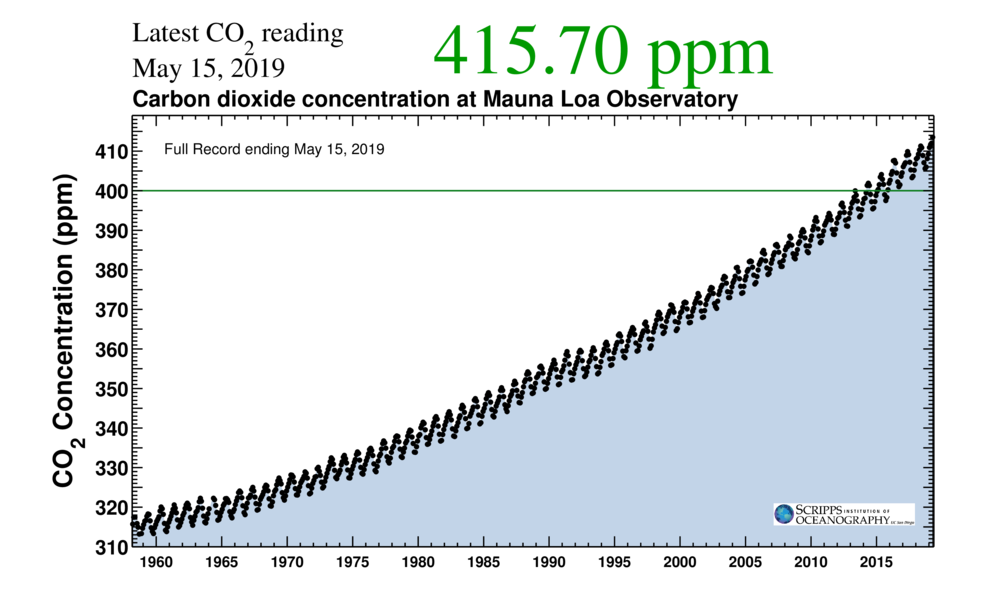
\includegraphics[scale = 0.3]{carbon.png}}
\end{center}
\begin{center}
\begin{tabular}{|c|c|c|c|c|c|c|}
\hline
Years passed since 1960 & 0 & 5 & 10 & 15 & 20 & 25 \\
\hline
$CO_2$ level (ppm) & 317 & 320 & 326 & 331 & 339 & 346 \\
\hline
Years passed since 1960 & 30 & 35 & 40 & 45 & 50 & 55\\
\hline
$CO_2$ level (ppm) & 354 & 361 & 370 & 380 & 390 & 401\\
\hline
\end{tabular}
\end{center}
(Data from: \href{ftp://aftp.cmdl.noaa.gov/products/trends/co2/co2_annmean_mlo.txt}{NOAA})
\end{Exercise}

\begin{Exercise}
Radioactive decay is modelled by $N = N_0e^{-kt}$, where $N_0$ and $k$ are the initial concentration and the decay constant respectively. While the expression is exponential, not linear, the technique of linear fit can still be applied if the data undergoes linearization. Show that by the substitution $n = \ln N$ the equation can be transformed into a linear equation $n = \ln N = \ln N_0 - kt = n_0 - kt$. Hence find the best linear fit on $(t, n)$ by finding the parameters $(n_0, k)$ from the experimental data on the radioactive isotope Sodium-24 below and recover the decay constant and initial mass.
\begin{center}
\begin{tabular}{|c|c|c|c|c|c|c|}
\hline
Time passed (hr) & 6 & 8 & 12 & 24 & 36 & 48\\
\hline
Mass (g) & 75.8 & 69.1 & 57.3 & 33.0 & 18.8 & 10.8\\
\hline
\end{tabular}
\end{center}
\end{Exercise}


\chapter{Discrete Fourier Transform}
We now discuss a powerful mathematical tool that can be approached from a least-square approximation view point. In last sections, we see how to fit a polynomial curve to some data. It is natural to ask, if there are any other types of curves that can be fitted to our interests. In the area of Earth Science, many phenomena can be described by the notion of waves, which are generally sinusoidal, e.g. atmospheric wave, seismic wave, electromagnetic wave. Hence, we may want to investigate if we can interpolate some data by using sines and cosines, and this is the central idea of what is known as Fourier Transform.

\section{Background and Types of Discrete Fourier Transform}
Fourier Transform and other related results are supported by the Fourier Theorem, which suggests that a function can be approximated by the sum of some sine-cosine series under some conditions. This implies that we can decompose a function into different sinusoidal waves, each having a certain amplitude, or called the Fourier coefficient. The resultant series has the name Fourier Series.
\begin{thm}
A periodic, smooth function $f(x)$ in the interval $[0,2\pi]$ can be approximated by the Fourier Series
\begin{align*}
S(f(x)) &= C_0 + A_1 \cos(x) + A_2 \cos(2x) + \cdots + B_1 \sin(x) + B_2 \sin(2x) + \cdots \\
&= C_0 + \sum_{k=1}^{\infty} (A_k \cos(kx) + B_k \sin(kx))
\end{align*}
\end{thm}
For a function that has an interval $[a,b]$ not exactly the same as $[0,2\pi]$, we can always scale it by replacing $x$ by the substitution $x' = 2\pi(\frac{x-a}{b-a})$. For non-periodic function over a fixed interval, we can extend it so that it behaves like a periodic one, by copying and pasting the same function over and over periodically.\\
\\
Here we provide a well-known example, the Fourier Series of $f(x) = x$ over $[0, 2\pi]$. We omit the calculation, and the answer is
\begin{align*}
S(x) &= \pi - 2 \sum_{k=1}^{\infty} \frac{\sin(kx)}{k} \\
&= \pi - 2 (\sin(x) + \frac{1}{2} \sin(2x) + \frac{1}{3} \sin(3x) + \cdots)
\end{align*}

\subsection{Discrete Fourier Transform, Real}
In Earth Science, and other fields like Engineering, often we are not given a function that has an analytical form to work with. Instead, we collect data from measurements at a fixed sampling rate, and what we obtain is a discrete time series. However, we can still apply the ideas of Fourier, and try to approximate and interpolate the finite time series with sinusoidal waves. Assume that, we have $n$ data points collected for the time series $f(t)$, evenly spaced at time $t = 0, 1, 2, \cdots, n-1$. We can scale the time range to $[0,2\pi]$ as what is suggested above, by making a change of variable $t' = 2\pi \frac{t}{n}$.\\
\\
Then, we can search a way to express the time series with sines and cosines of different frequencies like $\sin(t') = \sin((\frac{2\pi}{n})t), \sin(2t') = \sin((\frac{2\pi}{n})2t), \cdots$, and $\cos(t') = \cos((\frac{2\pi}{n})t), \cos(2t') = \cos((\frac{2\pi}{n})2t), \cdots$. The corresponding frequencies are $\frac{2\pi}{n}, 2(\frac{2\pi}{n}), \cdots$. In general, we propose an approximated form up to order $m$ as
\begin{align*}
S(f(t)) &= C_0 + A_1\cos((\frac{2\pi}{n})t) + A_2\cos((\frac{2\pi}{n})2t) + \cdots + A_m\cos((\frac{2\pi}{n})mt)\\
&\quad + B_1\sin((\frac{2\pi}{n})t) + B_2\sin((\frac{2\pi}{n})2t) + \cdots + B_m\sin((\frac{2\pi}{n})mt)\\
&= C_0 + \sum_{k=1}^{m} \left[A_k \cos((\frac{2\pi kt}{n})) + B_k \sin((\frac{2\pi kt}{n}))\right]
\end{align*}
Assume that we only use a few of sines and cosines for the approximation, such that the order $m$ much is less than the number of data points $n$, specifically, $2m+1 \leq n$. The least-square method is then set to find the best-fit parameters $C_0, A_1, B_1, \cdots, A_m, B_m$ for the system $G\vec{\beta} = \vec{d}$, where
\begin{align*}
G =
\begin{bmatrix}
1 & 1 & 0 & \cdots & 1 & 0 \\
1 & \cos(\frac{2\pi}{n}) & \sin(\frac{2\pi}{n}) & \cdots & \cos(\frac{2\pi m}{n}) & \sin(\frac{2\pi m}{n}) \\
1 & \cos(\frac{2\pi(2)}{n}) & \sin(\frac{2\pi(2)}{n}) & \cdots & \cos(\frac{2\pi (2m)}{n}) & \sin(\frac{2\pi (2m)}{n}) \\
\vdots & \vdots & \vdots & & \vdots & \vdots \\
1 & \cos(\frac{2\pi(n-1)}{n}) & \sin(\frac{2\pi(n-1)}{n}) & \cdots & \cos(\frac{2\pi (n-1)m}{n}) & \sin(\frac{2\pi (n-1)m}{n}) \\
\end{bmatrix}
\end{align*}
is a $n \times (2m+1)$ matrix and
\begin{align*}
&\vec{\beta} = 
\begin{bmatrix}
C_0 \\
A_1 \\
B_1 \\
\vdots \\
A_m \\
B_m
\end{bmatrix}
&\vec{d} = 
\begin{bmatrix}
f(0) \\
f(1) \\
f(2) \\
\vdots \\
f(n-1)
\end{bmatrix}
\end{align*}
are vectors with $2m+1$ and $n$ entries respectively. From theorem \ref{bestfit}, we know that the best parameters are found by
\begin{align*}
\vec{\beta_f} = (G^TG)^{-1}G^T\vec{d}
\end{align*}
However, we can greatly simplify the expression, by noticing that every column vector of sine/cosine is orthogonal to each other. If we write each sine-cosine term as a complex exponential using Euler's formula in definition \ref{Euler}, then each column vector of a sine-cosine pair in $G$ with a frequency of $2\pi k/n$, where both $k$ and $n$ are integers, can be expressed by the real and imaginary parts of
\begin{align*}
\left[\exp(\imath \frac{2\pi k}{n} t)\right]_{t = 0,1,2,\cdots,n-1}
&= \left[\cos(\frac{2\pi k}{n} t) + \imath\sin(\frac{2\pi k}{n} t) \right]_{t = 0,1,2,\cdots,n-1}
\end{align*}
or in the other way around,
\begin{align*}
\left[\exp(-\imath \frac{2\pi k}{n} t)\right]_{t = 0,1,2,\cdots,n-1}
&= \left[\cos(\frac{2\pi k}{n} t) - \imath\sin(\frac{2\pi k}{n} t) \right]_{t = 0,1,2,\cdots,n-1}
\end{align*}
We now first prove that the two column vectors of a sine-cosine pair that has the same frequency are orthogonal. We take the sum of squares of the first expression, which gives
\begin{align*}
\sum_{t=0}^{n-1} (\exp(\imath \frac{2\pi k}{n} t))^2 &= \sum_{t=0}^{n-1} (\cos(\frac{2\pi k}{n} t) + \imath\sin(\frac{2\pi k}{n} t))^2 \\
\sum_{t=0}^{n-1} \exp(\imath \frac{4\pi k}{n} t) &= \sum_{t=0}^{n-1} (\cos^2(\frac{2\pi k}{n} t) + 2\imath\sin(\frac{2\pi k}{n} t)\cos(\frac{2\pi k}{n} t) - \sin^2(\frac{2\pi k}{n} t))
\end{align*}
Notice that the left hand side is a geometric sequence with a common ratio $r = \exp(\imath 4\pi k/n)$, whose sum is seen to be
\begin{align*}
\frac{1-r^n}{1-r} &= \frac{1 - \exp(\imath 4\pi k)}{1 - \exp(\imath 4\pi k/n)} = 0
\end{align*}
as $\exp(\imath 4\pi k)$ is just $1$. By comparing the real and imaginary parts, we know that
\begin{align*}
\sum_{t=0}^{n-1} \cos^2(\frac{2\pi k}{n} t) &= \sum_{t=0}^{n-1} \sin^2(\frac{2\pi k}{n} t) \\
\sum_{t=0}^{n-1} \sin(\frac{2\pi k}{n} t)\cos(\frac{2\pi k}{n} t) &= 0
\end{align*}
The second equation shows that the two column vectors representing the sine and cosine wave of the same frequency have a dot product of zero and hence are orthogonal.\\
\\
Utilizing the complex formulations, we can also prove that column vectors of sine/cosine waves with different frequencies are orthogonal as well. Here we prove one of the cases, where the first wave is a sine a frequency of $2\pi k/n$, and the second wave is also a sine, of a frequency of $2\pi l/n$, where $k \neq l$ are both integers. We start by considering the sum of products between
\begin{align*}
\left[\exp(\imath \frac{2\pi k}{n} t)\right]_{t = 0,1,2,\cdots,n-1} = \left[\cos(\frac{2\pi k}{n} t) + \imath\sin(\frac{2\pi k}{n} t) \right]_{t = 0,1,2,\cdots,n-1}   
\end{align*}
and
\begin{align*}
\left[\exp(\imath \frac{2\pi l}{n} t)\right]_{t = 0,1,2,\cdots,n-1} = \left[\cos(\frac{2\pi l}{n} t) + \imath\sin(\frac{2\pi l}{n} t) \right]_{t = 0,1,2,\cdots,n-1}   
\end{align*}
The results are similar to the above analysis. Particularly,
\begin{align*}
\sum_{t=0}^{n-1} \cos(\frac{2\pi k}{n} t)\cos(\frac{2\pi l}{n} t) - \sum_{t=0}^{n-1} \sin(\frac{2\pi k}{n} t)\sin(\frac{2\pi l}{n} t) &= 0 
\end{align*}
We can also consider another dot product between $\left[\exp(\imath \frac{2\pi k}{n} t)\right]_{t = 0,1,2,\cdots,n-1}$ and
\begin{align*}
\left[\exp(-\imath \frac{2\pi l}{n} t)\right]_{t = 0,1,2,\cdots,n-1} = \left[\cos(\frac{2\pi l}{n} t) - \imath\sin(\frac{2\pi l}{n} t) \right]_{t = 0,1,2,\cdots,n-1}       
\end{align*}
This yields another relation as
\begin{align*}
\sum_{t=0}^{n-1} \cos(\frac{2\pi k}{n} t)\cos(\frac{2\pi l}{n} t) + \sum_{t=0}^{n-1} \sin(\frac{2\pi k}{n} t)\sin(\frac{2\pi l}{n} t) &= 0 
\end{align*}
From the two derived equations, we can conclude that
\begin{align*}
\sum_{t=0}^{n-1} \sin(\frac{2\pi k}{n} t)\sin(\frac{2\pi l}{n} t) &= 0    
\end{align*}
The orthogonality relations can be proven for sine vs cosine/cosine vs cosine of different frequencies as well. We will now establish the last result, the dot product of any cosine/sine column vector with a specific frequency $2\pi k/n$ with itself. We can consider the sum of products between
$\left[\exp(\imath \frac{2\pi k}{n} t)\right]_{t = 0,1,2,\cdots,n-1}$ and $\left[\exp(-\imath \frac{2\pi k}{n} t)\right]_{t = 0,1,2,\cdots,n-1}$. This time, the left hand side is not a geometric series, but rather $n$ terms of $1$. The relation is
\begin{align*}
\sum_{t=0}^{n-1} \cos^2(\frac{2\pi k}{n} t) + \sum_{t=0}^{n-1} \sin^2(\frac{2\pi k}{n} t) &= \sum_{t=0}^{n-1} \exp(\imath \frac{2\pi k}{n} t)\exp(-\imath \frac{2\pi k}{n} t) \\
&= \sum_{t=0}^{n-1} (1) \\
&= n
\end{align*}
Actually it roots from the fact that the sum of a sine-cosine square pair is $1$. Not long before, we have arrived at the equation
\begin{align*}
\sum_{t=0}^{n-1} \cos^2(\frac{2\pi k}{n} t) &= \sum_{t=0}^{n-1} \sin^2(\frac{2\pi k}{n} t)     
\end{align*}
Solving the two equations yields
\begin{align*}
\sum_{t=0}^{n-1} \cos^2(\frac{2\pi k}{n} t) &= \sum_{t=0}^{n-1} \sin^2(\frac{2\pi k}{n} t) = \frac{n}{2}    
\end{align*}
Hence the product $G^TG$, where each entry will be the dot products between vectors of sines and cosines, will be
\begin{align*}
G^TG =
\begin{bmatrix}
n & 0 & 0 & \cdots \\
0 & \frac{n}{2} & 0 & \\
0 & 0 & \frac{n}{2} & \\
\vdots & & & \ddots
\end{bmatrix}
\end{align*}
and
\begin{align*}
(G^TG)^{-1} = \frac{1}{n}
\begin{bmatrix}
1 & 0 & 0 & \cdots \\
0 & 2 & 0 & \\
0 & 0 & 2 & \\
\vdots & & & \ddots
\end{bmatrix}    
\end{align*}
So the best-fit parameters are
\begin{align*}
\vec{\beta_f} &= (G^TG)^{-1}G^T\vec{d} \\
\begin{bmatrix}
C_0 \\
A_1 \\
B_1 \\
\vdots \\
\end{bmatrix}
&= \frac{1}{n} 
\begin{bmatrix}
1 & 0 & 0 & \cdots \\
0 & 2 & 0 & \\
0 & 0 & 2 & \\
\vdots & & & \ddots
\end{bmatrix} 
\begin{bmatrix}
1 & 1 & 1 & \cdots \\
1 & \cos(\frac{2\pi}{n}) & \cos(\frac{2\pi(2)}{n}) & \\
0 & \sin(\frac{2\pi}{n}) & \sin(\frac{2\pi(2)}{n}) &  \\
\vdots & & & \ddots
\end{bmatrix}
\begin{bmatrix}
f(0)\\
f(1)\\
f(2)\\
\vdots
\end{bmatrix} \\
\begin{bmatrix}
C_0 \\
A_1 \\
B_1 \\
\vdots \\
\end{bmatrix}
&= 
\frac{1}{n}
\begin{bmatrix}
1 & 1 & 1 & \cdots \\
2 & 2\cos(\frac{2\pi}{n}) & 2\cos(\frac{2\pi(2)}{n}) & \\
0 & 2\sin(\frac{2\pi}{n}) & 2\sin(\frac{2\pi(2)}{n}) &  \\
\vdots & & & \ddots
\end{bmatrix}
\begin{bmatrix}
f(0)\\
f(1)\\
f(2)\\
\vdots
\end{bmatrix} 
\end{align*}
Detailed expressions are
\begin{align*}
C_0 &= \frac{1}{n}(f(0) + f(1) + f(2) + \cdots + f(n-1)) \\
&= \frac{1}{n}\sum_{t=0}^{n-1} f(t) \\
A_m &= \frac{2}{n}(f(0) + f(1)\cos(\frac{2\pi m}{n}) + \cdots + f(n-1)\cos(\frac{2\pi (n-1)m}{n})) \\
&= \frac{2}{n}\sum_{t=0}^{n-1} f(t)\cos(\frac{2\pi mt}{n}) \\
B_m &= \frac{2}{n}(f(1)\sin(\frac{2\pi m}{n}) + \cdots + f(n-1)\sin(\frac{2\pi (n-1)m}{n})) \\
&= \frac{2}{n}\sum_{t=0}^{n-1} f(t)\sin(\frac{2\pi mt}{n})
\end{align*}

\begin{exmp}
\label{ex11.2.1}
Fit the following time-series with sinusoidal waves up to order $m=1$. $f(0) = 1, f(1) = 4, f(2) = 6, f(3) = 3, f(4) = 5$.\\
\\
The order $m=1$ means that there are only three constituents, which are the constant term, and a sine-cosine pair with a frequency of $\frac{2\pi k}{n}$ where $k=1$, $n=5$. The best-fit parameters will be
\begin{align*}
\begin{bmatrix}
C_0 \\
A_1 \\
B_1
\end{bmatrix}
&= 
\frac{1}{5}
\begin{bmatrix}
1 & 1 & 1 & 1 & 1 \\
2 & 2\cos(\frac{2\pi}{5}) & 2\cos(\frac{2\pi(2)}{5}) & 2\cos(\frac{2\pi(3)}{5}) & 2\cos(\frac{2\pi(4)}{5}) \\
0 & 2\sin(\frac{2\pi}{5}) & 2\sin(\frac{2\pi(2)}{5}) & 2\sin(\frac{2\pi(3)}{5}) & 2\sin(\frac{2\pi(4)}{5})
\end{bmatrix}
\begin{bmatrix}
f(0)\\
f(1)\\
f(2)\\
f(3)\\
f(4)
\end{bmatrix} 
\end{align*}
\begin{align*}
C_0 &= \frac{1}{5} (1+4+6+3+5) = \frac{19}{5} \\
A_1 &= \frac{2}{5} (1 + 4\cos(\frac{2\pi}{5}) + 6\cos(\frac{2\pi(2)}{5}) + 3\cos(\frac{2\pi(3)}{5}) + 5\cos(\frac{2\pi(4)}{5})) \\
&= -\frac{7}{5} \\
B_1 &= \frac{2}{5} (4\sin(\frac{2\pi}{5}) + 6\sin(\frac{2\pi(2)}{5}) + 3\sin(\frac{2\pi(3)}{5}) + 5\sin(\frac{2\pi(4)}{5})) \\
&\approx 0.325
\end{align*}
So the best sinusoidal fit of order $m=1$ for the time-series concerned is
\begin{align*}
f(t) = \frac{19}{5} - \frac{7}{5} \cos(\frac{2\pi}{5}t) + 0.325 \sin(\frac{2\pi}{5}t)
\end{align*}
Short Exercise: Find an improved approximation with order $m = 2$.
\end{exmp}

However, there are two problems with the formulation. First, since we may want to make the approximation as good as possible, we have to know how high the order $m$ needs to be. Let's continue with the assumption that the time step is $1$, so that the sampling points are at $t = 0, 1, 2, \cdots, n-1$. Then the Nyquist Sampling Theorem tells us that there is a cap for $m$.
\begin{thm}
For a evenly spaced time-series that has a time step of $1$, any wave with a linear frequency $f > f_{ny} = 1/2$ or angular freqency $\omega > \omega_{ny} = \pi$ cannot be detected. More generally, for a time step of $\Delta t$, the Nyquist frequnecy is $\omega_{ny} = \frac{\pi}{\Delta t}$.
\end{thm}
So it means that we only need the sines/cosines up to the order $m_c$, where $m_c$ is inferred by looking at the expression of angular frequency inside the expression of sines/cosines, that is
\begin{align*}
\frac{2\pi m}{n} \leq \frac{2\pi m_c}{n} &= \pi \\
m \leq m_c &= \frac{n}{2}
\end{align*}
\paragraph{Proof} We illustrate a portion of the theorem by proving
\begin{align*}
\cos(\frac{2\pi (m_c + (m_c - m))}{n}) &= \cos(\frac{2\pi (m_c - (m_c - m))}{n}) \\
&= \cos(\frac{2\pi m}{n})
\end{align*}
so that mirroring $m$ about $m_c$ has no effect on the cosine wave. But the left hand side is simply
\begin{align*}
\cos(\frac{2\pi (m_c + (m_c - m))}{n}) &= \cos(\frac{4\pi mc}{n} - \frac{2\pi m}{n}) \\
&= \cos(\frac{4\pi (n/2)}{n} - \frac{2\pi m}{n}) \\
&= \cos(2\pi - \frac{2\pi m}{n}) \\
&= \cos(\frac{2\pi m}{n})
\end{align*}

For $n$ is even, then we have frequencies from zero to $m_c = n/2$. Notice that the zero frequency constant term contributes a single parameter, every other frequencies contribute two parameters as sines/cosines, and the maximum frequency $m_c = n/2$ only contributes one parameter of cosine (the corresponding diagonal entry for $(G^TG)^{-1}$ will be $1/n$ instead of $2/n$), as the sine function will be always zero at that frequency. This means that there are $n$ parameters as total.\\
\\
For $n$ is odd, the situation is the same except at the maximum frequency $m_c = (n-1)/2$ which contributes two parameters as a sine-cosine pair. Counting also reveals that the amount of parameters is also $n$. In both cases, there can be at most $n$ sinusoidal curves for fitting $n$ data points. Since the amount of parameters is the same as the number of data, it becomes an interpolation that passes through all the given data points, and this forms the foundation of Discrete Fourier Transform. But the difference between odd/even $n$ has to be remembered when we are tackling the maximum frequency signal. \\
\\
Another drawback of the approach is that it uses sine-cosine pairs for computation. In \autoref{section:complexno}, we have learnt the power of complex exponentials to simultaneously represent sines and cosines. Therefore, one may explore the possibility of using complex exponentials to do Discrete Fourier Transform. This has the benefits of simplicity and also convenience when programming.

\subsection{Discrete Fourier Transform, Complex}

Now extending the ideas from the last section, we propose an interpolation scheme which uses $\exp(\imath\frac{2\pi k}{n}t)$, for a time-series with $n$ data, evenly spaced by a time step of $1$. The range of $k$ will be from $-\frac{n}{2}, -(\frac{n}{2}-1), \cdots, 0, \frac{n}{2}-1$ for even $n$ and $-\frac{n-1}{2}, -(\frac{n-1}{2}-1), \cdots, 0, \frac{n-1}{2}$ for odd $n$. Both ranges ensure that the total number of sinusoidal waves used is exactly $n$.\\
\\
Each pair of $k$ and $-k$, or $\exp(\imath\frac{2\pi k}{n}t)$, and $\exp(-\imath\frac{2\pi k}{n}t)$ in combination, gives rise to $\cos(\frac{2\pi k}{n}t)$ and $\sin(\frac{2\pi k}{n}t)$ by properties \ref{sincoscomplex}, and so we see the correspondence between the real and complex version of Discrete Fourier Transform.\\
\\
Now, the matrix $G$ has the form of
\begin{align*}
G =
\begin{bmatrix}
1 & 1 & \cdots & 1 & 1 & \cdots\\
1 & \exp(\imath\frac{2\pi}{n}) & \cdots & \exp(\imath\frac{2\pi(n/2-1)}{n}) & \exp(\imath\frac{2\pi(-n/2)}{n}) & \cdots \\
1 & \exp(\imath\frac{2\pi(2)}{n}) & \cdots & \exp(\imath\frac{2\pi(n/2-1)(2)}{n}) & \exp(\imath\frac{2\pi(-n/2)(2)}{n}) & \cdots\\
\vdots & \vdots & & \vdots & \vdots & \\
1 & \exp(\imath\frac{2\pi(n-1)}{n}) & \cdots & \exp(\imath\frac{2\pi(n/2-1)(n-1)}{n}) & \exp(\imath\frac{2\pi(-n/2)(n-1)}{n}) & \cdots
\end{bmatrix}
\end{align*}
for even $n$, where each column representing frequencies that have $k = 0, 1, \cdots, \frac{n}{2}-1$, $-\frac{n}{2}, \cdots, -1$. This is a common convention where we starts from $k = 0$, and increases to the largest positive $k$, then flips the sign and resumes from the largest negative $k$, goes all the way back to $k = -1$. Odd $n$ has a similar form of $G$, but with all the $k$ replaced by the appropriate integer range.\\
\\
Notice that as we are now working with complex matrices, the normal equation is modified and the formula of the best-fit parameters are now $\vec{\beta}_f = (G^*G)^{-1}G^*\vec{d}$, contrary to theorem \ref{bestfit} as the transpose is replaced by conjugate transpose/Hermitian. The entries of $G^*G$ are the complex dot products between the column vectors of $G$.\\
\\
The orthogonality relation between different column vectors of complex exponentials is very easy to find. The procedure is similar to what we have done when proving the orthogonality for the real case, but even less tedious. The key point is to write the complex dot product along the two columns as a geometric sequence, that when the values of $k$ are different, will be evaluated to zero. The readers are invited to verify this result, as well as the fact that the complex dot product between any column vector of complex exponentials and itself is $n$. Thus, the expression $G^*G$ is just $nI$, and $(G^*G)^{-1} = \frac{1}{n} I$.\\
\\
Now we denote the best-fit parameters, or coefficients by $C_k$. Subsequently,
\begin{align*}
\vec{\beta}_f &= (G^*G)^{-1}G^*\vec{d} \\
&= \frac{1}{n}G^*\vec{d} \\
\begin{bmatrix}
C_0 \\
C_1 \\
\vdots \\
C_{n/2-1} \\
C_{-n/2} \\
\vdots
\end{bmatrix}
&= 
\frac{1}{n}
\begin{bmatrix}
1 & 1 & 1 & \cdots \\
1 & \exp(-\imath\frac{2\pi}{n}) & \exp(-\imath\frac{2\pi(2)}{n}) & \cdots \\
\vdots & \vdots & \vdots & \\
1 & \exp(-\imath\frac{2\pi(n/2-1)}{n}) & \exp(-\imath\frac{2\pi(n/2-1)(2)}{n}) & \cdots \\
1 & \exp(-\imath\frac{2\pi(-n/2)}{n}) & \exp(-\imath\frac{2\pi(-n/2)(2)}{n}) & \cdots 
\end{bmatrix}
\begin{bmatrix}
f(0) \\
f(1) \\
f(2) \\
\vdots
\end{bmatrix}
\end{align*}
Again this is for even $n$, we ought to replace the coefficients and complex exponentials appropriately for odd $n$. We now conclude the method of Complex Discrete Fourier Transform in a compact way as follows.
\begin{defn}
The coefficients, or amplitudes, of the Discrete Fourier Transform in complex form are
\begin{align*}
C_k = \sum_{t=0}^{n-1} f(t)\exp(-\imath\frac{2\pi k}{n}t)
\end{align*}
where $n$ is the number of data. $k$ are all integers ranging from $[-\frac{n}{2}, \frac{n}{2}-1]$ for even $n$, and $[-\frac{n-1}{2}, \frac{n-1}{2}]$ for odd $n$. The negative sign in the complex exponentials comes from the conjugate transpose in the formulation. In the most common convention the factor $1/n$ is removed. For a time step $\Delta t$ different from $1$, the expression is
\begin{align*}
C_k = \sum_{t=0}^{n-1} f(t)\exp(-\imath\frac{2\pi k}{n\Delta t}t)
\end{align*}
We will denote the series of $C_k$ by $F(k)$ or $\hat{f}(k)$.
\end{defn}
The relation between $C_k$ and the parameters $A_k$, $B_k$ in the real counterpart are inferred from properties \ref{sincoscomplex} and comparing the expression for the real case, that is
\begin{align*}
A_k &= \frac{C_k + C_{-k}}{n} \\
B_k &= -\frac{(C_k - C_{-k})}{n\imath}
\end{align*}
for $k \neq 0$. A closer inspection reveals that, since sine is an odd function, and cosine is an even function, $\Re(C_k) = \Re(C_{-k})$, and $\Im(C_k) = -\Im(C_{-k})$, or in other words, $C_k$ and $C_{-k}$ are a pair of complex conjugate. And so the relation between the real and complex Discrete Fourier Transform is
\begin{proper}
\label{FTrealcomplex}
The amplitudes $A_k$, $B_k$ in real Discrete Fourier Transform, and $C_k$ in complex Discrete Fourier Transform satisfy
\begin{align*}
A_k &= 2\Re(C_k)/n \\
B_k &= -2\Im(C_k)/n
\end{align*}
\end{proper}

\begin{exmp}
Find the Complex Discrete Fourier Transform for the time-series in example \ref{ex11.2.1}.\\
\\
Using the formula above, we have
\begin{align*}
C_0 &= 1+4+6+3+5 = 19 \\
C_1 &= 1 + 4\exp(-\imath\frac{2\pi}{5}) + 6\exp(-\imath\frac{2\pi(2)}{5}) + 3\exp(-\imath\frac{2\pi(3)}{5}) + 5\exp(-\imath\frac{2\pi(4)}{5}) \\
&= -3.5 - 0.812\imath \\
C_2 &= 1 + 4\exp(-\imath\frac{2\pi(2)}{5}) + 6\exp(-\imath\frac{2\pi(2)(2)}{5}) \\
&\quad+ 3\exp(-\imath\frac{2\pi(2)(3)}{5}) + 5\exp(-\imath\frac{2\pi(2)(4)}{5}) = -3.5 + 3.441 \imath
\end{align*}
$C_{-1}$ and $C_{-2}$ are complex conjugates of $C_1$ and $C_2$ respectively. \\
Short Exercise: Check if properties \ref{FTrealcomplex} is true in this example.
\end{exmp}

We can also undo the Discrete Fourier Transform and recover the initial time-series by its inverse, defined as follows.
\begin{defn}
The inverse Discrete Fourier Transform is done by
\begin{align*}
f(t) &= \frac{1}{n}\sum_{k=0}^{n-1} F(k)\exp(\imath\frac{2\pi k}{n}t)
\end{align*}
Sometimes we use the symbol $F^{-1}$ to denote the inverse operation.
\end{defn}

\section{Convolution}
Convolution is often used in the world of Fourier Transform due to a beautiful theorem that will be introduced later. In the area of Earth Science, as well as Physics and Statistics, convolution also has a place, for describing phenomena, or their solutions. Now we will introduce how convolution in a discrete sense is defined first, and a daily example will be provided as an illustration.\\
\\
Discrete Convolutions always involved two time-series as below.
\begin{defn}
The convolution $h(t)$ between two discrete time-series $f(t)$ and $g(t)$ is written $f(t) * g(t)$, defined as
\begin{align*}
h(t) = f(t) * g(t) = \sum_{\tau=-\infty}^{\infty} f(\tau) g(t-\tau)
\end{align*}
if $\tau$ takes a value so that the index in either $f$ or $g$ is out of the range, then the term becomes zero.
\end{defn}
For instance, if $f(t)$ is defined from $t = 0$ and $t = 4$ and $g(t)$ is defined from $t = 0$ and $t = 6$, then
\begin{align*}
h(0) &= f(0)g(0) \\
h(1) &= f(0)g(1-0) + f(1)g(1-1) = f(0)g(1) + f(1)g(0) \\
h(4) &= f(0)g(4-0) + f(1)g(4-1) + f(2)g(4-2) + f(3)g(4-3) + f(4)g(4-4) \\
&= f(0)g(4) + f(1)g(3) + f(2)g(2) + f(3)g(1) + f(4)g(0)
\end{align*}
and
\begin{align*}
h(6) &= f(0)g(6) + f(1)g(5) + f(2)g(4) + f(3)g(3) + f(4)g(2) \\
h(9) &= f(3)g(6) + f(4)g(5) \\
h(10) &= f(4)g(6)
\end{align*}
It can be deduced that the resulted convolution will has a length of $m + n - 1$ if the two input time-series have a length of $m$ and $n$.

\begin{exmp}
The probability of Mary getting married within some years can be described by the time-series $q(t)$, where
\begin{align*}
q(t) = 
\begin{cases}
0.2 & 0 \leq t \leq 2 \\
0.1 & 3 \leq t \leq 6 \\
0 & t \geq 7
\end{cases}
\end{align*}
The probability $r(t)$ that Mary gives birth to a baby some years $t$ after marriage is
\begin{align*}
r(t) = 
\begin{cases}
0 & t = 0 \\
0.15 & 1 \leq t \leq 4 \\
0.08 & 5 \leq t \leq 9 \\
0 & t \geq 10
\end{cases}    
\end{align*}
Find the net probability of Mary getting a baby at some years $t$ from now on, assuming she will only get pregnant after married. \\
\\
We identify the required probability $p(t) = q(t) * r(t)$ is a convolution between $q(t)$ and $r(t)$, which effectively have a length of $7$ and $9$. Particularly, taking $t = 5$ as an example, then we have
\begin{align*}
p(t = 5) &= P(\text{Birth 5 years later}|\text{Married now})P(\text{Married now}) \\
&\quad+ P(\text{Birth 4 years later}|\text{Married 1 year later})P(\text{Married 1 year later})\\
&\quad+ \cdots \\
&\quad+ P(\text{Birth 1 year later}|\text{Married 4 years later})P(\text{Married 4 years later}) \\
&= q(0)r(5) + q(1)r(4) + q(2)r(3) + q(3)r(2) + q(4)r(1) \\
&= (0.2)(0.08) + (0.2)(0.15) + (0.2)(0.15) + (0.1)(0.15) + (0.1)(0.15) \\
&= 0.106
\end{align*}
where $P(A|B)$ is the probability of getting $A$ when $B$ happens.\\
Short Exercise: Find the chance of Mary getting a baby at $8$ years later by convolution.
\end{exmp}

If, the two discrete time-series are infinitely long, then we have the following weaker version of Convolution Theorem for discrete Fourier Transform.
\begin{thm}
For two infinitely long discrete time-series $f(t)$ and $g(t)$, we have
\begin{align*}
F[f(t) * g(t)](k) &= \hat{f}(k)\hat{g}(k)
\end{align*}
The Discrete Fourier Transform of the convolution between the two time-series is equal to the product of the two Discrete Fourier Transforms for their own.
\end{thm}
It is worth emphasized again that this is a much weaker statement compared to the full form, which is known as the Circular Convolution Theorem, that do the convolution for two finite time-series in a cyclic manner, and works in two directions.

\section{Exercise}
\begin{Exercise}
Carry out Discrete Fourier Transform for the following data.
\begin{center}
\begin{tabular}{|c|c|c|c|c|c|c|}
\hline
unit time & 0 & 1 & 2 & 3 & 4 \\
\hline
f(t) & 4 & 6 & 7 & 1 & 3  \\
\hline
unit time & 5 & 6 & 7 & 8 & 9 \\
\hline
f(t) & 2 & 3 & 5 & 2 & 6\\
\hline
\end{tabular}
\end{center}
Find the amplitude and phase of the sinusoidal wave corresponding to an angular frequency of $2\pi\frac{3}{10}$. 
\end{Exercise}

\begin{Exercise}
Download an \href{https://cds.climate.copernicus.eu/cdsapp#!/dataset/reanalysis-era5-single-levels?tab=overview}{ERA5 Temperature Dataset} over any time period of $5$ years. Select a location as you like, and extract the temperature time-series there. Apply Discrete Fourier Transform on the time series, and identify any dominant frequency or time period whose amplitude (the magnitude of complex coefficient) is large. Explain the peaks with Earth Science knowledge.
\end{Exercise}

\begin{Exercise}
Perform Fourier Transform on the time-series of the first Principal Direction in exercise (10.5).
\end{Exercise}
\chapter{Numerical Integration}

Sometimes, the integral of a function may have an analytical solution. However, for more complicated functions, closed-form solution is often unavailable or very difficult to obtain. In Earth Science or other Science fields, integrals that are hard to evaluate are not rare. The most common example is the integral of a Gaussian function
\begin{align*}
\int_{-\infty}^{t} e^{-\tau^2/(2\sigma^2)} d\tau
\end{align*}
that frequently appears as the cumulative distribution function of Normal Distribution. Sometimes we also need to calculate an integral from limited measurements. This forces us to apply \textit{Numerical Integration} methods to do the integration in a discrete manner. In the age of computers, this approach is feasible in many cases, as it can usually give an accurate estimate on the actual value of the integral.\\
\\
While integration methods themselves are not directly related to linear algebra, vectors and matrices provide a compact description to some of them, Therefore, they are worth to be mentioned, accounting for their importance in Earth Science.

\section{One-dimensional Numerical Integration}
We start from the simplest case, numerical integration for single integrals.

\subsection{Trapezoidal Rule}
The most straight-forward method is to go back to the definition of integral itself. Since integral can be regarded to be the sum of infinitely many small rectangles, we can approximate any integral by partitioning the area into some finite amount of rectangles, hoping the accuracy is not too bad. This method has the name \textit{Rectangle Rule}.\\
\\
We will not talk about the Rectangle Rule in details. Instead, we jump to an improved version which is a natural generalization of the Rectangle Rule. Often while using Rectangle Rule, we craft the rectangle with a height that is either the value of the function at the left (or right) interval. So, the approximation by rectangles will introduce substantial errors due to the difference between their heights and the right (left) intervals. We naturally amend this by using a trapezoid that touches the function at both intervals. This is called the \textit{Trapezoidal Rule}.\\
\begin{defn}
\label{1301}
The Trapezoidal Rule approximates an integral by
\begin{align*}
\int_a^b f(x) dx \approx \sum_{k=0}^{n-1} \frac{h}{2} (f(x_k) + f(x_{k+1}))  
\end{align*}
where we partition the interval $[a,b]$ into $n$ intervals evenly at $x_0, x_1, \cdots, x_n$ with a width of $h$. Expanding the summation gives
\begin{align*}
&\quad \sum_{k=0}^{n-1} \frac{h}{2} (f(x_k) + f(x_{k+1})) \\
&= \frac{h}{2} (f(x_0) + 2f(x_1) + 2f(x_2) + \cdots + 2f(x_{n-2}) + 2f(x_{n-1}) + f(x_n))
\end{align*}
\end{defn}

\begin{exmp}
Integrate $\cos(0.7\pi x)$ numerically by Trapezoidal Rule over $x = [0,2]$.\\
\\
We divide the interval into $5$ sub-intervals with a spacing of $h = 0.4$, $x_0 = 0, x_1 = 0.4, x_2 = 0.8, \cdots, x_5 = 2$. By definition \ref{1301}, we obtain an estimate of
\begin{align*}
&\quad \int_0^2 \cos(0.7\pi x) dx \\
&\approx \frac{0.4}{2} [\cos(0.7\pi (0)) + 2\cos(0.7\pi (0.4)) + 2\cos(0.7\pi (0.8))\\
&\quad + 2\cos(0.7\pi (1.2)) + 2\cos(0.7\pi (1.6)) + \cos(0.7\pi (2))] \\
&\approx -0.404
\end{align*}
The exact value is around $-0.432$.
\end{exmp}

\subsection{Simpson's Rule}
An even more powerful numerical integration method is to used quadratic curves to approximate the area under the curve. Different from Trapezoidal Rule, each quadratic curve used span two sub-intervals, so the total number of sub-intervals must be even. (If it is odd, then we can use Trapezoidal Rule for the last sub-interval.) This is known as the \textit{Simpson's Rule}.
\begin{defn}
\label{1302}
The Simpson's Rule approximates an integral by
\begin{align*}
\int_a^b f(x) dx \approx \sum_{l=0}^{m-1} \frac{2h}{6} (f(x_{2l}) + 4f(x_{2l+1}) + f(x_{2l+2}))  
\end{align*}
assuming the number of sub-interval over $[a,b]$ is even, $n = 2m$. Again each of them has a even spacing of $h$. Alternatively, we have
\begin{align*}
&\quad \sum_{l=0}^{m-1} \frac{2h}{6} (f(x_{2l}) + 4f(x_{2l+1}) + f(x_{2l+2})) \\
&= \frac{2h}{6} (f(x_0) + 4f(x_1) + 2f(x_2) + 4f(x_3) + \cdots + 2f(x_{n-2}) + 4f(x_{n-1}) + f(x_n))
\end{align*}
\end{defn}

\begin{exmp}
Integrate $f(x) = e^{-x}$ between $[0,1]$ using Simpson's Rule.\\
\\
We demonstrate by dividing the interval into $10$ sub-intervals with a width of $h=0.1$ and there are $5$ quadratic curves used for the estimation. From the $(1, 4, 2, 4, 1)$ pattern in definition \ref{1302}, we have
\begin{align*}
&\quad \int_0^1 e^{-x} dx \\
&\approx \frac{2(0.1)}{6}(e^0 + 4e^{-0.1} + 2e^{-0.2} + 4e^{-0.3} + 2e^{-0.4} \\
&\quad + 4e^{-0.5} + 2e^{-0.6} + 4e^{-0.7} + 2e^{-0.8} + 4e^{-0.9} + e^{-1}) \\
&\approx 0.63212
\end{align*}
The answer is very close to the exact value, with the first difference occurs at the $7$-th decimal place.\\ 
Short Exercise: Repeat the approximation with Trapezoidal Rule.
\end{exmp}

\section{Generalization and Discussion}
\subsection{Multi-dimensional Numerical Integration}
It can be inferred from the previous example that the two numerical integration methods above can be written in the form of dot product for single integrals. For Trapezoidal Rule, it is 
\begin{align*}
\frac{h}{2}
\begin{bmatrix}
f(x_0) & f(x_1) & f(x_2) & \cdots & f(x_{n-1}) & f(x_n)
\end{bmatrix}
\begin{bmatrix}
1 \\
2 \\
2 \\
\vdots \\
2 \\
1
\end{bmatrix}
\end{align*}
While for Simpson's Rule, it is
\begin{align*}
\frac{2h}{6}
\begin{bmatrix}
f(x_0) & f(x_1) & f(x_2) & f(x_3) & f(x_4) & \cdots & f(x_{n-2}) & f(x_{n-1}) & f(x_n)
\end{bmatrix}
\begin{bmatrix}
1 \\
4 \\
2 \\
4 \\
2 \\
\vdots \\
2 \\
4 \\
1
\end{bmatrix}
\end{align*}
Generalizing for the double integral of a function $f(x,y)$, the expression becomes a quadratic form. the Trapezoidal Rule has a form of
\begin{align*}
(\frac{h_x}{2})(\frac{h_y}{2})
\begin{bmatrix}
1 & 2 & 2 & \cdots & 1
\end{bmatrix}
\begin{bmatrix}
f(x_0,y_0) & f(x_1, y_0) & f(x_2, y_0) & \cdots & f(x_n, y_0) \\
f(x_0,y_1) & f(x_1, y_1) & f(x_2, y_1) & \cdots & \\
f(x_0,y_2) & f(x_1, y_2) & f(x_2, y_2) & \cdots & \\
\vdots & & & \ddots & \\
f(x_0,y_m) & & & & f(x_n,y_m)
\end{bmatrix}
\begin{bmatrix}
1 \\
2 \\
2 \\
\vdots \\
1
\end{bmatrix}   
\end{align*}
where $m$ and $n$ are the amounts of sub-intervals along $y$ and $x$-directions. Simpson's Rule for double integrals reads
\begin{align*}
(\frac{2h_x}{6})(\frac{2h_y}{6})
\begin{bmatrix}
1 & 4 & 2 & \cdots & 1
\end{bmatrix}
\begin{bmatrix}
f(x_0,y_0) & f(x_1, y_0) & f(x_2, y_0) & \cdots & f(x_n, y_0) \\
f(x_0,y_1) & f(x_1, y_1) & f(x_2, y_1) & \cdots & \\
f(x_0,y_2) & f(x_1, y_2) & f(x_2, y_2) & \cdots & \\
\vdots & & & \ddots & \\
f(x_0,y_m) & & & & f(x_n,y_m)
\end{bmatrix}
\begin{bmatrix}
1 \\
4 \\
2 \\
\vdots \\
1
\end{bmatrix}   
\end{align*}
assuming the step width $h_x$ and $h_y$ along the $x$ and $y$-direction. This is effectively equivalent to first apply the method in $x$/$y$-direction and then apply it again in $y$/$x$-direction.

\begin{exmp}
Numerically integrate the double integral $\int_1^4 \int_0^3 e^{-x}\cos(y) dxdy$ over the rectangular region $0 \leq x \leq 3$, $1 \leq y \leq 4$.\\
\\
We employ the Trapezoidal Rule with a step size of $h = 1$ along both $x$ and $y$-directions. From the formula above, we know that the approximation is given by
\begin{align*}
(\frac{1}{2})^2
\begin{bmatrix}
1 & 2 & 2 & 1
\end{bmatrix}
\begin{bmatrix}
e^{-0}\cos(1) & e^{-1}\cos(1) & e^{-2}\cos(1) & e^{-3}\cos(1) \\
e^{-0}\cos(2) & e^{-1}\cos(2) & e^{-2}\cos(2) & e^{-3}\cos(2) \\
e^{-0}\cos(3) & e^{-1}\cos(3) & e^{-2}\cos(3) & e^{-3}\cos(3) \\
e^{-0}\cos(4) & e^{-1}\cos(4) & e^{-2}\cos(4) & e^{-3}\cos(4) 
\end{bmatrix}
\begin{bmatrix}
1 \\
2 \\
2 \\
1
\end{bmatrix}       
\end{align*}
\end{exmp}
The value of this quadratic form is $-1.5039$, compared to the exact value of $-1.5187$.\\
Short Exercise: Use two-dimensional Simpson's Rule to compute this double integral again.\\
\\
The ideas for extending these two rules for triple integrals are similar. The integration methods are applied in the three directions, one after another. The formula can be expressed using tensors, which will be taught in the last chapter.

\subsection{Error Estimates}
Errors of Trapezoidal Rule is proportional to the square of step size, while Simpson’s Rule has an error proportional to the fourth power of step size. In general, Simpson’s Rule is more accurate. Below listed the detailed error estimates for these two methods in one-dimensional cases.
\begin{proper}
Given a definite, single integral of a function $f(x)$ to be numerically integrated over the region $[a,b]$, the maximum error incurred by Trapezoidal Rule is
\begin{align*}
\abs{E_T} \leq \frac{Q_2(b-a)}{12}h^2
\end{align*}
where $h$ is the step size, $Q_2$ is the absolute value of the maximum second derivative of the function, $\abs{f''(x)}$, in the range. Error of Simpson's Rule is bounded by
\begin{align*}
\abs{E_S} \leq \frac{Q_4(b-a)}{180}h^4
\end{align*}
$Q_4$ is similarly the absolute value of the maximum fourth derivative of the function, $\abs{f^{(4)}(x)}$.
\end{proper}
The actual error is usually much smaller than the theoretical bound. As a final note, Trapezoidal Rule and Simpson’s Rule belong to a wider class of integration formula called \textit{Newton-Cotes Quadrature Rule}.

\section{Exercise}

\begin{Exercise}
Use Trapezoidal Rule and Simpson's Rule to numerically integrate $\int_0^{8} \exp(-\frac{x^2}{8^2}) dx$. The spacing between each sampling point should be less than $1$. It is given that the value of the integral is about $5.97459306$, estimate the percentage errors of these two numerical integration methods.
\end{Exercise}

\begin{Exercise}
Use Trapezoidal Rule and Simpson's Rule to numerically integrate $\int_2^{10}\int_2^{10} \ln(x)\sqrt{y} dxdy$. The spacing between each grid point should be less than $1$.
\end{Exercise}

\begin{Exercise}
What is the error of Simpson's Rule if we integrate $f(x) = x^3 + 2x^2 + 3x + 4$ between $[0, 10]$?
\end{Exercise}
\chapter{Markov Chain}

In Earth Science, we often look at the time evolution of some variables, like temperature, rainfall etc. Sometimes, the variables can be modelled as random variables. A simple daily example will be tossing a coin (no matter it is fair or not), where the outcomes (head/tail) are probabilistic. Some Earth System examples are the chances of extreme weathers, or some slow geological processes. Such processes involving random variables are known as \textit{Stochastic Processes}, and we will visit the related Statistical concepts. Particularly, we will investigate the so-called \textit{Markov Chain}, which assumes the present state of a stochastic process only depends on the past. Modelling a stochastic process with Markov Chain can give more satisfactory results when it is believed that the process inherently correlates strongly with previous states, or is said to be have \textit{memory}.

\section{Basic Statistical Ideas for Markov Chain}

\subsection{Lagged Auto-correlation}

First, let's talk about how we determine if a time-series possesses some sorts of memory. Memory causes the past of a time-series to influence the present, and hence will leave a mark when we try to correlate the past and the present of the time-series. Here comes the idea of \textit{Lagged Auto-correlation}, which is the correlation between a time-series and itself, but one of them is lagged and shifted by a certain amount of days, $k$ (The direction of shifting does not matter much, and we only care about the overlapping part), and it is more specifically known as the \textit{Lag-k Auto-correlation}.

\begin{defn}
\label{1403}
The lag-k auto-correlation $r_k$ of a time-series $\{x\}$ is defined as
\begin{align*}
r_k &= \frac{\sum_{i=1}^{n-k}(x_i - \bar{x}_{-})(x_{i+k} - \bar{x}_{+})}{\sqrt{(\sum_{i=1}^{n-k}(x_i - \bar{x}_{-})^2) (\sum_{i=k+1}^{n}(x_i - \bar{x}_{+})^2)}}
\end{align*}
where $\{x_{-}\}$ and $\{x_{+}\}$ denotes the sequence representing the earliest and latest $n-k$ data. An overline denotes an average. Alternatively, the formula can be written as
\begin{align*}
r_k &= \frac{\text{Cov}(\{x_{-}\},\{x_{+}\})}{\sqrt{\text{Var}(\{x_{-}\}) \text{Var}(\{x_{+}\})}} \\
&= \frac{\text{Cov}(\{x_{-}\},\{x_{+}\})}{\sqrt{\text{Cov}(\{x_{-}\}, \{x_{-}\}) \text{Cov}(\{x_{+}\}, \{x_{+}\})}}
\end{align*}
where the definitions of variance and covariance are those from definitions \ref{variance} and \ref{covariance}.
\end{defn}
If the lag-k auto-correlation of a time-series is close to $1$ or $-1$, it means that the state at a certain time will probably lead to a similar/opposite state $k$ time steps later.

\begin{exmp}
For the traffic flow data over some seven days of a highway below, find its lag-1 auto-correlation.
\begin{center}
\begin{tabular}{|c|c|c|c|c|c|c|c|}
\hline
Day & 1 & 2 & 3 & 4 & 5 & 6 & 7 \\
\hline
Vehicles per Hour & 680 & 820 & 760 & 790 & 840 & 1030 & 1080 \\
\hline
\end{tabular}
\end{center}
We first locate the first and last $7-1 = 6$ data as two smaller time-series, which are $\{x_-\} = \{680, 820, 760, 790, 840, 1030\}$ and $\{x_+\} = \{820, 760, 790, 840, 1030, 1080\}$. The sample variances of the two time-series are
\begin{align*}
\text{Cov}(\{x_-\}) &= 13720 \text{ (Vehicles per Hour)}^2 \\
\text{Cov}(\{x_+\}) &= 17987 \text{ (Vehicles per Hour)}^2
\end{align*}
and their sample covariance is
\begin{align*}
\text{Cov}(\{x_{-}\},\{x_{+}\}) &= 12000 \text{ (Vehicles per Hour)}^2
\end{align*}
The readers are encouraged to verify the numbers. Hence by the formula above, the lag-1 auto-correlation is
\begin{align*}
r_1 &= \frac{12000}{\sqrt{13720*17987}} = 0.7639
\end{align*}
It means that a busy traffic will likely be followed by a more or less busy traffic the next day, which is not unreasonable.\\
Short Exercise: Compute the lag-2 auto-correlation.
\end{exmp}

\subsection{Conditional Probabilities, Stochastic Matrices}
To fully understand Markov Chain, we also need to know what conditional probabilities are. The \textit{Conditional Probability} $P(A|B)$ is the probability of event $A$ occurring given event $B$ has occurred. For an evolving system which has a finite amount of states and can only possesses one state at a time, e.g. on-and-off, the conditional probability $P(A_i^{[k+1]}|A_j^{[k]})$ represents the probability of state $A_i$ occurring at time step $k+1$ if the state is $A_j$ at time step $k$. An Atmospheric Science example is daily weather reports, which in a simplistic sense, can be sunny, rainy, windy. If it is rainy today, then there is a relatively high chance it is rainy tomorrow, i.e. $P(\text{rainy}^{[k+1]}|\text{rainy}^{[k]})$ is high.\\
\\
For $N$ finite, distinct events in a well-defined, closed system, so that the system always take one and only one of the events as its state, we have the following observation.
\begin{thm}
The sum of conditional probabilities for a changing system with $N$ mutually exclusive (only one state at a time) and exhaustive (the states cover all possibilities) events $A_1, A_2, \cdots, A_N$, we have
\begin{align*}
\sum_{i=1}^N P(A_i^{[k+1]}|A_j^{[k]}) &= P(A_1^{[k+1]}|A_j^{[k]}) + P(A_2^{[k+1]}|A_j^{[k]}) + \cdots + P(A_N^{[k+1]}|A_j^{[k]}) \\
&= 1
\end{align*}
where $k$ denotes a particular time step. It means that any given event $A_j$ must consequently lead to one of possible states (including $A_j$ itself) at the next time step.
\end{thm}
As a result, we can express conditional probabilities $P(A_i^{[k+1]}|A_j^{[k]})$ for a particular $A_j$ in a system using a column vector with entries that sum up to $1$. Using daily weather as an example, assumed there are only three states (sunny/windy/rainy), if a sunny day has a chance of $0.8$ to be followed by another sunny day, and $0.15$/$0.05$ for another windy/rainy day. Then we can write
\begin{center}
\begin{tabular}{|c|c|}
\hline
k+1 $\backslash$ k & Sunny \\
\hline
Sunny & 0.8 \\
\hline
Windy & 0.15 \\
\hline 
Rainy & 0.05 \\
\hline
\end{tabular}
\end{center}
as a column vector
\begin{align*}
\begin{bmatrix}
0.8 \\
0.15 \\
0.05
\end{bmatrix}
\end{align*}
We can do the same for the other two states. If a windy day has a probability of $0.2$/$0.5$/$0.3$ leading to a sunny/windy/rainy day, and a rainy day has a chance of $0.1$/$0.2$/$0.7$ leading to a sunny/windy/rainy day, then
\begin{center}
\begin{tabular}{|c|c|c|c|}
\hline
k+1 $\backslash$ k & Sunny & Windy & Rainy \\
\hline
Sunny & 0.8 & 0.2 & 0.1\\
\hline
Windy & 0.15 & 0.5 & 0.2 \\
\hline 
Rainy & 0.05 & 0.3 & 0.7 \\
\hline
\end{tabular}
\end{center}
can be summarized by the so-called \textit{Stochastic Matrix} as
\begin{align*}
P = 
\begin{bmatrix}
0.8 & 0.2 & 0.1\\
0.15 & 0.5 & 0.2 \\
0.05 & 0.3 & 0.7
\end{bmatrix}
\end{align*}
\begin{defn}
\label{1401}
The stochastic matrix for a closed system with mutually exclusive and exhaustive events $A_1, A_2, \cdots, A_N$, is
\begin{align*}
P =
\begin{bmatrix}
P(A_1^{[k+1]}|A_1^{[k]}) & P(A_1^{[k+1]}|A_2^{[k]}) & \cdots & P(A_1^{[k+1]}|A_N^{[k]})\\
P(A_2^{[k+1]}|A_1^{[k]}) & P(A_2^{[k+1]}|A_2^{[k]}) & & \\
\vdots & & \ddots & \\
P(A_N^{[k+1]}|A_1^{[k]}) & & & P(A_N^{[k+1]}|A_N^{[k]})
\end{bmatrix}
\end{align*}
where $P_{ij}$ is the conditional probability of moving to state $i$ at the next time step from the present state $j$.
\end{defn}
Notice that the entries along any column add up to $1$. Column $j$ holds the conditional probabilities of state $j$ leading to different states at the next time step.

\section{Markov Chain}

\subsection{State Vector, Steady State}

Processes can be represented by such stochastic matrices are called Markov Chains. It is assumed that the conditional probabilities outlined in the stochastic matrices do not change in time. Given a probability vector (or the \textit{State Vector}) $\vec{x}^{[k]}$ consisting of the probabilities of having different states at a certain time step $k$, we can calculate the probability vector $\vec{x}^{[k+1]}$ at the next time step $k+1$ as $P\vec{x}^{[k]}$.

\begin{proper}
Given a Markov Chain, with a stochastic matrix $P$ described in \ref{1401}, then the state vector $\vec{x}^{[k+1]}$ at time step $k+1$ is decided by
\begin{align*}
\vec{x}^{[k+1]} &= P\vec{x}^{[k]}   
\end{align*}
\end{proper}
\paragraph{Proof} If we look at the $i$-th entry at both sides, we have
\begin{align*}
\vec{x_i}^{[k+1]} &= P_{i1} \vec{x_1}^{[k]} + P_{i2} \vec{x_2}^{[k]} + P_{i3} \vec{x_3}^{[k]} \cdots 
\end{align*}
or more explicitly
\begin{align*}
P(A_i^{[k+1]}) &= P(A_i^{[k+1]}|A_1^{[k]}) P(A_1^{[k]}) + P(A_i^{[k+1]}|A_2^{[k]}) P(A_2^{[k]}) + \cdots \\
&= \sum_{j=1}^N P(A_i^{[k+1]}|A_j^{[k]}) P(A_j^{[k]})
\end{align*}
This result is essentially a manifestation of the \textit{Law of Total Probability}. In our circumstance, it holds as the events are mutually exclusive and exhaustive, and hence the property as well.\\
\\
Similarly, at time step $k+2$ the probability vector is $\vec{x}^{[k+2]} = P^2\vec{x}^{[k]}$. $\vec{x}^{[1]} = P\vec{x}^{[0]}, \vec{x}^{[2]} = P\vec{x}^{[1]} = P(P\vec{x}^{[0]}) = P^2\vec{x}^{[0]}, \cdots, \vec{x}^{[n]} = P^n\vec{x}^{[0]}$.

\begin{exmp}
\label{1402}
Using the previous example of weather, the stochastic matrix is
\begin{align*}
P = 
\begin{bmatrix}
0.8 & 0.2 & 0.1\\
0.15 & 0.5 & 0.2 \\
0.05 & 0.3 & 0.7
\end{bmatrix}   
\end{align*}
Find the probabilities of each type of weather occurring on Day 2, if we somehow know that the chances of being sunny/windy/rainy on Day 1 is $0.3$/$0.4$/$0.3$. \\
\\
By the formula we have just obtained, the required state vector is
\begin{align*}
\vec{x}^{[2]} &= P\vec{x}^{[1]} \\
&=
\begin{bmatrix}
0.8 & 0.2 & 0.1\\
0.15 & 0.5 & 0.2 \\
0.05 & 0.3 & 0.7
\end{bmatrix}   
\begin{bmatrix}
0.3 \\
0.4 \\
0.3
\end{bmatrix} \\
&= 0.3
\begin{bmatrix}
0.8 \\
0.15 \\
0.05
\end{bmatrix}
+ 0.4
\begin{bmatrix}
0.2 \\
0.5 \\
0.3
\end{bmatrix}
+ 0.3
\begin{bmatrix}
0.1 \\
0.2 \\
0.7
\end{bmatrix} \\
&=
\begin{bmatrix}
0.35 \\
0.305 \\
0.345
\end{bmatrix}
\end{align*}
So on Day 2, the chances of sunny/windy/rainy are $0.35$/$0.305$/$0.345$. It is emphasized in the last step that the required state vector at the next day is just the linear combination of the conditional probability column vectors, with the weighting specified by the current state vector. It is again the Law of Total Probability working.\\
Short Exercise: Find the state vector on the next day if today is windy.
\end{exmp}

For a Markov Chain which has been ongoing for a long period of time, and the initial state becomes effectively forgotten (\textit{Memoryless}), it is desirable to obtain the steady state vector which represents the probability of every state given no prior knowledge of initial state. The steady state vector $\vec{q}$ is one that remains the same for any time step. Hence we have $\vec{q} = P\vec{q} = ... = P^n\vec{q}$.\\
\\
Rearrangement gives $(I-P)q = 0$, in which the steady-state vector $\vec{q}$ corresponds to the eigenvector of $P$ when eigenvalue is $1$. $\vec{q}$ is then calculated following the usual procedure for solving the linear system and computing the eigenvector.
\begin{defn}
The steady state of a Markov Chain is simply the eigenvector of the identity matrix minus its stochastic matrix $I - P$ that corresponds to the eigenvalue of $1$, and divided by the sum of entries so that they add up to $1$.
\end{defn}

\begin{exmp}
Continuing the last example, 
\begin{align*}
P = 
\begin{bmatrix}
0.8 & 0.2 & 0.1\\
0.15 & 0.5 & 0.2 \\
0.05 & 0.3 & 0.7
\end{bmatrix}   
\end{align*}
and
\begin{align*}
I - P = 
\begin{bmatrix}
0.2 & -0.2 & -0.1\\
-0.15 & 0.5 & -0.2 \\
-0.05 & -0.3 & 0.3
\end{bmatrix}   
\end{align*}
A simple calculation reveals that the eigenvector of $I - P$ for $\lambda=1$ is $(\frac{9}{7}, \frac{11}{14}, 1)^T$. Since the probabilities have to be added up to $1$, dividing each component by the sum yields the steady state vector $\vec{q} = (\frac{18}{43}, \frac{11}{43}, \frac{14}{43})^T \approx (0.419, 0.256, 0.326)^T$, meaning that there is $41.9\% / 25.6\% / 32.6\%$ chance of having a sunny/windy/rainy day on average.
\end{exmp}

\subsection{Expected Value Problem}
For the special case in which one of the states in Markov Chain is absorbing, i.e. no outgoing pathway and the probability to remain in the node/state is 1, all pathway will eventually lead to accumulation in this particular sink. This is referred to as an \textit{Absorbing Markov Chain} and it is possible to predict the expected time needed for any state to arrive at the absorbing state.\\
\\
We can attack this problem by finding the total expected time spent in other non-absorbing nodes, which is precisely the very same quantity we want to know. At the zeroth time step, or $T=0$, the time spent in the starting node and other nodes is one and zero unit time respectively. (We can adapt for the case where the starting condition is probabilistic, e.g. $50\%$ chance in the first node and $50\%$ chance in the second node.) At $T=k$, the average time spent during the $k$-th time step in different nodes are exactly the probabilities to land on these nodes after $k$ time steps.\\
\\
Hence the idea is to add up the time staying in every non-absorbing node over every time step. Therefore, we consider the variant of the stochastic matrix in which the row and column of the absorbing state is deleted. Assume that there are three states in the absorbing Markov Chain, and its stochastic matrix is
\begin{align*}
P &= 
\begin{bmatrix}
0.2 & 0.8 & 0\\
0.7 & 0 & 0 \\
0.1 & 0.2 & 1
\end{bmatrix}
\end{align*}
The third column shows that the third node is an absorbing node. After deleting the row and column related to the absorbing state, and only looking at those non-absorbing states, we have
\begin{align*}
P_0 &= 
\begin{bmatrix}
0.2 & 0.8\\
0.7 & 0 \\
\end{bmatrix}   
\end{align*}
Assume we starts at the first node, i.e. the probability vector representing the initial state is $(1, 0)^T$ in this case, the formula to calculating the total staying time over all time steps would be
\begin{align*}
I
\begin{bmatrix}
1 \\
0
\end{bmatrix}
+
P
\begin{bmatrix}
1 \\
0
\end{bmatrix}
+
P^2
\begin{bmatrix}
1 \\
0
\end{bmatrix}
+ \cdots 
=
(1 + P_0 + P_0^2 + \cdots)
\begin{bmatrix}
1 \\
0
\end{bmatrix}
=
\begin{bmatrix}
T_1 \\
T_2
\end{bmatrix}
\end{align*}
where the first term at the left hand side is the staying time at zeroth time step, the second term is that at first time step, and so on. $T_1$ and $T_2$ will be the total expected time spent at node $1$ and $2$. We can utilize the formula of geometric sum for matrices, and generalize the formula to accommodate more states.
\begin{proper}
The expected time for a initial state in a Markov Chain to be absorbed in the sink (assumed that there is only one sink) can be inferred from the relation
\begin{align*}
\begin{bmatrix}
T_1 \\
T_2 \\
T_3 \\
\cdots
\end{bmatrix}
=
(I - P_0)^{-1}
\vec{x_0}^{[0]}
\end{align*}
where P is the associated stochastic matrix and $P_0$ is $P$ with the row and column of the absorbing state taken away. $\vec{x_0}^{[0]}$ is the initial state vector, also with the entry corresponding to the absorbing node removed. The required expected absorption time is the sum of $T_i$, over all possible $i$. 
\end{proper}
The only caveat is that the formula of geometric sum for matrices may not be true, just like the original formula for numbers will fail if the common ratio has a magnitude larger than or equal to $1$. However, it is guaranteed for a well-behaved stochastic matrix without isolated loops, $(I - P_0)^{-1} = 1 + P_0 + P_0^2 + \cdots$ indeed holds.
\begin{exmp}
For the absorbing Markov Chain we have been discussing about, which has
\begin{align*}
P_0 &= 
\begin{bmatrix}
0.2 & 0.8\\
0.7 & 0 \\
\end{bmatrix}   
\end{align*}
We have
\begin{align*}
I - P_0 &= 
\begin{bmatrix}
0.8 & -0.8\\
-0.7 & 1 \\
\end{bmatrix} \\
(I - P_0)^{-1} &= 
\begin{bmatrix}
4.166 & 3.333 \\
2.917 & 3.333
\end{bmatrix} \\
(I - P_0)^{-1}\vec{x_0}^{[0]} &= 
\begin{bmatrix}
4.166 & 3.333 \\
2.917 & 3.333
\end{bmatrix}
\begin{bmatrix}
1 \\
0
\end{bmatrix} 
=
\begin{bmatrix}
4.166 \\
2.917
\end{bmatrix}
\end{align*}
Hence the expected time required to reach the third node starting from the first node will be just the sum of the first column in $P_0$, $4.166 + 2.917 = 7.083$.\\
Short Exercise: Find the expected time required to reach the third node if it has $50\%/50\%$ chances to start at the first/second node instead.
\end{exmp}

\subsection{Auto-correlation Predicted by Markov Chain}

The last topic we will touch about Markov Chain is its inherent auto-correlation. Consider the simplest case, where a Markov Chain only has two possible states, with a $2 \times 2$ stochastic matrix, having the form
\begin{align*}
P = 
\begin{bmatrix}
P_{11} & P_{12} \\
P_{21} & P_{22}
\end{bmatrix}
\end{align*}
Assume the first/second state represents a value of $1$/$0$ without the loss of generality. The theoretical lag-1 auto-correlation between the binary states, predicted by the Markov Chain, is definition \ref{1403} modified appropriately, that is
\begin{align*}
r_1 &= \frac{\text{Cov}(\{x_{-}\},\{x_{+}\})}{\sqrt{\text{Var}(\{x_{-}\}) \text{Var}(\{x_{+}\})}} \\
&= \frac{E(X_{-}X_{+}) - E(X_{-})E(X_{+})}{\sqrt{(E(X_{-}^2) - (E(X_{-}))^2)(E(X_{+}^2) - (E(X_{+}))^2)}}
\end{align*}
where we have used the short-cut formula for variance and covariance listed in section \ref{variancesec}. If the Markov Chain operates for a long enough time, then the average of the two time-series lagged by a day will be equal, implying that
\begin{align*}
E(X_{-}) = E(X_{+}) &= q_1
\end{align*}
where $\vec{q}$ is the stationary state vector, with $q_1$ being the stationary probability of being in state $1$. Similarly, we have
\begin{align*}
E(X_{-}^2) = E(X_{+}^2) &= q_1    
\end{align*}
since the square of an individual $1$/$0$ time-series will return itself. The remaining job is to determine $E(X_{-}X_{+})$, which is simply
\begin{align*}
E(X_{-}X_{+}) &= P(x_{+}=1 \text{ and } x_{-}=1) \\
&= P(x_{+}=1|x_{-}=1) P(x_{-}=1) \\
&= P_{11} q_1
\end{align*}
So the lag-1 auto-correlation is
\begin{align*}
r_1 &= \frac{(P_{11}q_1-q_1^2)}{\sqrt{(q_1-q_1^2)(q_1-q_1^2)}} \\
&= \frac{q_1(P_{11}-q_1)}{(q_1-q_1^2)} \\
&= \frac{P_{11}-q_1}{1-q_1}
\end{align*}
But, by the eigenvector definition of the stationary state, we have
\begin{align*}
P_{11}q_1 + P_{12}q_2 &= q_1 \\
P_{11}q_1 + P_{12}(1-q_1) &= q_1 \\
(1 - P_{11} + P_{12}) q_1 &= P_{12}
\end{align*}
Substituting this into the formula of lag-1 auto-correlation, we arrive at
\begin{align*}
r_1 &= \frac{(1 - P_{11} + P_{12})(P_{11}-q_1)}{(1 - P_{11} + P_{12})(1-q_1)} \\
&= \frac{P_{11}(1 - P_{11} + P_{12}) - (1 - P_{11} + P_{12})q_1}{1 - P_{11} + P_{12} - (1 - P_{11} + P_{12})q_1} \\
&= \frac{P_{11}(1 - P_{11} + P_{12}) - P_{12}}{1 - P_{11} + P_{12} - P_{12}} \\
&= \frac{(1-P_{11})(P_{11}-P_{12})}{1 - P_{11}} \\
&= P_{11} - P_{12}
\end{align*}
Therefore, the magnitude of lag-1 auto-correlation estimated from Markov Chain is simply the difference between the two conditional probabilities on the same row in the stochastic matrix. By the same essence, the lag-k auto-correlation can be inferred from $r_k = Q_{11} - Q_{12}$, where $Q = P^k$. Fortunately, due to the structure of stochastic matrix, we have a very simple formula for lag-k auto-correlation, which is just the $k$-th power of the lag-1 auto-correlation, $r_k = r_1^k$.

\begin{proper}
The lag-k auto-correlation of a binary Markov Chain, with a stochastic matrix $P$, is
\begin{align*}
r_k = (P^k)_{11} - (P^k)_{12} = (P_{11} - P_{12})^k = r_1^k
\end{align*}
\paragraph{Proof} The formula holds for $k=1$ as we just see, now we will briefly prove the equality for $k = 2$.
\begin{align*}
P^2 &=
\begin{bmatrix}
P_{11} & P_{12} \\
P_{21} & P_{22} \\
\end{bmatrix}^2 \\
&= 
\begin{bmatrix}
P_{11} & P_{12} \\
1-P_{11} & 1-P_{12} \\
\end{bmatrix}
\begin{bmatrix}
P_{11} & P_{12} \\
1-P_{11} & 1-P_{12} \\
\end{bmatrix} \\
&=
\begin{bmatrix}
P_{11}^2 - P_{12}(1-P_{11}) & P_{11}P_{12} - P_12(1-P_{12}) \\
\cdots & \cdots \\
\end{bmatrix}
\end{align*}
So
\begin{align*}
(P^2)_{11} - (P^2)_{12} &= (P_{11}^2 - P_{12}(1-P_{11})) -  (P_{11}P_{12} - P_12(1-P_{12})) \\
&= P_{11}^2 - 2P_{11}P_{12} + P_{12}^2 \\
&= (P_{11} - P_{12})^2
\end{align*}
as we have asserted. Cases for $k \geq 3$ can be proved via Mathematical Induction.
\end{proper}
For instance, given a two-state Markov Chain with the stochastic matrix
\begin{align*}
P = 
\begin{bmatrix}
0.35 & 0.75 \\
0.65 & 0.25
\end{bmatrix}
\end{align*}
The lag-1 auto-correlation will be $0.35 - 0.75 = 0.25 - 0.65 = -0.4$, and the lag-4 auto-correlation will be $(-0.4)^4 = 0.0256$. Lag-k auto-correlation of any Markov Chain always decays exponentially.

\section{Exercise}

\begin{Exercise}
For the island Gu-Nei-Ng-Dou, if it is a sunny day, then the next day has $75\%$ chance of being sunny, $10\%$ chance of being windy, and $15\%$ of being rainy. Meanwhile, a windy day has $60\%$/$25\%$/$15\%$ chance leading to a sunny/windy/rainy day, and a rainy day has $30\%$/$20\%$/$50\%$ chance leading to a sunny/windy/rainy day. Find:
\begin{enumerate}[label=(\alph*)]
\item the probability of getting a rainy day three days after a rainy day,
\item the steady-state probability of all three types of weather,
\item the probability of getting at least one sunny day today and tomorrow if it is sunny yesterday.
\end{enumerate}
\end{Exercise}

\begin{Exercise}
Not all stochastic matrices are well-behaved (or formally, regular) Markov Chains. Consider the case where there exists three states, A, B, and C. State A always lead to state B, which in turn always lead to state C, and state C will always move back to state A. Construct the stochastic matrix for this case, and find its steady-state vector. Despite the existence of a steady-state vector, prove that it is an unstable, oscillating system by a counter-example, as well as an intuitive argument.
\end{Exercise}

\begin{Exercise}
For the carbon cycle below, calculate the rate constant $k$ for each transport process, and verify that on average it takes about 213000 years for carbon in the ocean reservoir to be buried in the sediment by (a) absorbing Markov Chain, (b) considering the biosphere-atmosphere-ocean as a single reservoir and calculating the lifetime $\tau = \frac{1}{k} = \frac{\text{total stock mass}}{\text{flux}}$. Also, if the pathway to sediment is neglected, find the steady-state vector of the biosphere-atmosphere-ocean system and confirm they are already in steady state as one would expect.
\begin{center}
\fbox{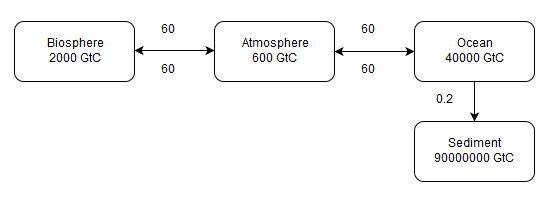
\includegraphics[scale = 0.5]{carboncycle.jpg}}
\end{center}
\end{Exercise}

\begin{Exercise}
Aftershocks can happen when an earthquake or another aftershock has occurred. Assume that the probability of aftershocks (rows) can be modelled such that it depends on the prior earthquake/aftershock only (columns), as the table shown below. Find the expected total number of earthquakes/aftershocks if there is an earthquake of magnitude 8.
\begin{center}
\begin{tabular}{|c|c|c|c|c|}
\hline
& M8 & M6-7 & M$\leq$5 & Stops\\
\hline
M8 & 0.1 & 0 & 0 & 0\\
\hline
M6-7 & 0.8 & 0.66 & 0 & 0\\
\hline
M$\leq$5 & 0.1 & 0.32 & 0.92 & 0\\
\hline
Stops & 0 & 0.02 & 0.08 & 1\\
\hline
\end{tabular}
\end{center}
Note: The numbers are made up and the real-world situation is much more complicated. Markov Chain can definitely be a tool for Seismology, but the usage will be more involved.
\end{Exercise}

\begin{Exercise}
Daniel is drunk at a bar. He wants to go to the train station so that he can go home. However, since he is drunk, he loses his sense of direction, and will move randomly along the green edge (shown in the map below) once at a time. Assume that at any starred location, the chances of moving to all other neighbouring locations are equal. Nevertheless, once he arrives at the train station, he will stop wandering and take the train. How many moves does it take on average for Daniel to reach the train station?
\begin{center}
(Placeholder for Diagram)
\end{center}
\end{Exercise}

\begin{Exercise}
Attempt \href{https://projecteuler.net/problem=84}{Project Euler Problem 84}, preferably with programming.
\end{Exercise}
\chapter{Matrix Factorization Methods}

In this chapter, we are going to discuss some matrix factorization methods. We have introduced one of them (QR Decomposition) in \autoref{chap:6}. In the past, matrix factorization is not a hot topic in Earth Science. However, as Machine Learning gains popularity in different Scientific fields, many Earth Science research starts to involve matrix factorization, which has been a main instrument in Machine Learning. Apart from this, a less visible usage of matrix factorization is embedded in the implementation of linear algebra package in programming languages (e.g. LAPACK, for Fortran). Those matrix factorization enables a much faster and stable computation of linear algebra problems, such as finding inverses or solving linear systems. Other potential applications include image processing, data compression, and more.

\section{Square Matrix Factorization}
\subsection{Cholesky Factorization}

\textit{Cholesky Decomposition} is for a special class of matrices which are symmetric and positive-definite. We have talked about how a matrix is positive-definite in section \ref{Conic}. For a symmetric and positive-definite matrix $A$, Cholesky Decomposition factorizes it into $U^TU$, where $U$ is an upper triangular matrix, $U^T$ is hence a lower triangular matrix. (Upper/lower triangular implies non-zero entries only present along or above/below the main diagonal) An example would be
\begin{align*}
A = 
\begin{bmatrix}
1 & 0 & 1 \\
0 & 1 & 1 \\
1 & 1 & 6
\end{bmatrix}
&=
\begin{bmatrix}
1 & 0 & 0 \\
0 & 1 & 0 \\
1 & 1 & 2
\end{bmatrix}
\begin{bmatrix}
1 & 0 & 1 \\
0 & 1 & 1 \\
0 & 0 & 2
\end{bmatrix} \\
&= 
\begin{bmatrix}
1 & 0 & 1 \\
0 & 1 & 1 \\
0 & 0 & 2
\end{bmatrix}^T
\begin{bmatrix}
1 & 0 & 1 \\
0 & 1 & 1 \\
0 & 0 & 2
\end{bmatrix} \\
&= U^TU 
\end{align*}

We can compute Cholesky Decomposition step by step, first rewriting the $n \times n$ matrix $A$ into the proposed factorized form of
\begin{align*}
A = U^T U = 
\begin{bmatrix}
u_{11} & \vec{r_1}^T \\
\vec{0} & U_b 
\end{bmatrix}^T
\begin{bmatrix}
u_{11} & \vec{r_1}^T \\
\vec{0} & U_b 
\end{bmatrix} = 
\begin{bmatrix}
u_{11} & \vec{0}^T \\
\vec{r_1} & U_b^T
\end{bmatrix}
\begin{bmatrix}
u_{11} & \vec{r_1}^T \\
\vec{0} & U_b 
\end{bmatrix}
\end{align*}
where $u_{11}$ is the first diagonal element of $U$, $\vec{r_1}$ is a column vector of length $n-1$ and $U_b$ is a block matrix with size $(n-1, n-1)$. The matrix dot product at R.H.S. gives
\begin{align*}
A = 
\begin{bmatrix}
\alpha_{11} & \vec{a_1}^T \\
\vec{a_1} & A_b 
\end{bmatrix}
=
\begin{bmatrix}
u_{11}^2 & u_{11}\vec{r_1}^T \\
u_{11}\vec{r_1} & \vec{r_1}\vec{r_1}^T + U_b^T U_b
\end{bmatrix}
= U^TU
\end{align*}
where $\alpha_{11}$ is the first diagonal element of $A$, $\vec{a_1}$ and $A_b$ is also a column vector just like $\vec{r_1}$ and $U_b$. The dot product involving block matrices is carried out just like usual matrix dot product. Comparing the both sides, we have
\begin{align*}
\alpha_{11} &= u_{11}^2 \\
\vec{a_1} &= u_{11}\vec{r_1} \\
A_b &= \vec{r_1}\vec{r_1}^T + U_b^T U_b
\end{align*}
\begin{align*}
u_{11} &= \sqrt{\alpha_{11}} \\
\vec{r_1} &= \frac{\vec{a_1}}{\sqrt{\alpha_{11}}} \\
U_b^T U_b &= A_b - \vec{r_1}\vec{r_1}^T
\end{align*}
By the relations above, we determine the first row and column of $U$. Subsequently, the remaining block $U_b$ is constructed by applying the same procedure on $A_2 = U_b^T U_b$ which has been obtained from the last relation, and then keep repeating the method to reduce the resulted block matrix on until the last entry is processed.
\begin{defn}
The Cholesky Factorization $U^TU$ of a symmetric, positive-definite matrix $A$, is constructed by the recursive relations
\begin{align*}
u_{mm} &= \sqrt{\alpha_{mm}} \\
\vec{r_m} &= \frac{\vec{a_m}}{\sqrt{\alpha_{mm}}} \\
U_b^T U_b &= A_b - \vec{r_m}\vec{r_m}^T
\end{align*}
where the subscript $m$ implies the $m$-th step. The formula are applied iteratively on $A_m = U_b^T U_b$ acquired at every step.
\end{defn}

\begin{exmp}
Perform Cholesky Factorization on the symmetric, positive-definite matrox
\begin{align*}
A &=
\begin{bmatrix}
4 & 2 & 0 \\
2 & 2 & 2 \\
0 & 2 & 5 
\end{bmatrix}
\end{align*}
The first step results in
\begin{align*}
u_{11} &= \sqrt{4} = \textcolor{red}{2} \\
\vec{r_1} &= \frac{1}{\sqrt{4}}
\begin{bmatrix}
2 \\
0
\end{bmatrix}
= 
\begin{bmatrix}
\textcolor{blue}{1} \\
\textcolor{blue}{0}
\end{bmatrix} \\
A_2 = U_b^T U_b &= 
\begin{bmatrix}
2 & 2 \\
2 & 5
\end{bmatrix}
-
\begin{bmatrix}
1 \\
0
\end{bmatrix}
\begin{bmatrix}
1 & 0
\end{bmatrix} \\
&= \begin{bmatrix}
1 & 2 \\
2 & 5 
\end{bmatrix}
\end{align*}
So we know that
\begin{align*}
U &=
\begin{bmatrix}
\textcolor{red}{2} & \textcolor{blue}{1} & \textcolor{blue}{0} \\
0 & ? & ? \\
0 & ? & ? \\
\end{bmatrix}
\end{align*}
The next iteration $A_2$ on gives
\begin{align*}
u_{22} &= \sqrt{1} = \textcolor{red}{1} \\  
\vec{r_2} &= \frac{1}{\sqrt{1}}
\begin{bmatrix}
2
\end{bmatrix}
=
\begin{bmatrix}
\textcolor{blue}{2}
\end{bmatrix} \\
U_b^T U_b &=
5 - 
\begin{bmatrix}
2
\end{bmatrix}
\begin{bmatrix}
2
\end{bmatrix} \\
&= 
\begin{bmatrix}
1
\end{bmatrix}
\end{align*}
We still need to deal with the $1 \times 1$ matrix that is left. At the third step, we simply take
\begin{align*}
u_{33} = \sqrt{1} = \textcolor{Green}{1}
\end{align*}
So the final expression of $U$ is given by
\begin{align*}
U = 
\begin{bmatrix}
2 & 1 & 0 \\
0 & \textcolor{red}{1} & \textcolor{blue}{2} \\
0 & 0 & \textcolor{Green}{1}
\end{bmatrix}
\end{align*}
Short Exercise: Check if $A = U^T U$.
\end{exmp}

\subsection{LU/LDU Factorization}

\textit{LU Factorization} is similar to Cholesky Factorization. It decomposes any matrix into one upper and one lower triangular matrix, but the original matrix needs not to be symmetric or positive-definite. The key to LU factorization is the method of Gaussian Elimination discussed in sections \ref{Echelon} and \ref{subsection:invGauss}. By Gaussian Elimination we can always reduce a given matrix to an upper triangular matrix (row echelon form), through a sequence of elementary row operations, or equivalently taking the dot product with a sequence of elementary matrices to the left. \\
\\
Denote such operations with $E_1', E_2', \cdots, E_n'$, in the spirit similar to theorem \ref{GaussElimPrinciple}, we have $E_n'\cdots E_2'E_1'A = U$, where $U$ is an upper triangular matrix produced from the forward phase of Gaussian Elimination. Rearrangement gives
\begin{align*}
A = (E_1'^{-1}E_2'^{-1}\cdots E_n'^{-1})U    
\end{align*}
If all $E_i'$ involves no row interchanges, then they would be all lower triangular matrices as required by the forward stage of Gaussian Elimination (if there is row interchange, then $E_i'$ will not be a lower triangular matrix.). As a result, $(E_1'^{-1}E_2'^{-1}\cdots E_n'^{-1})$ will be a lower triangular matrix $L$, and the LU Factorization $A = LU$ is constructed.
\begin{thm}
LU Factorization of a matrix $A$ is possible if it can be reduced to a row echelon form $U$, which will be an upper triangular matrix, by forward Gaussian Elimination. The steps and elementary matrices used to produce $U$ can be grouped together, and inverted to give a lower triangular matrix $L$. The LU Factorization will then be $A = LU$.
\end{thm}

\begin{exmp}
Compute a LU Factorization for
\begin{align*}
A = 
\begin{bmatrix}
2 & 0 & 0 \\
0 & 1 & 1 \\
2 & 0 & 4
\end{bmatrix}
\end{align*}
By Gaussian Elimination, we have
\begin{align*}
\begin{bmatrix}
2 & 0 & 0 \\
0 & 1 & 1 \\
2 & 0 & 4
\end{bmatrix}
&\rightarrow 
\begin{bmatrix}
1 & 0 & 0 \\
0 & 1 & 1 \\
2 & 0 & 4 
\end{bmatrix}
& E_1' =
\begin{bmatrix}
\frac{1}{2} & 0 & 0 \\
0 & 1 & 0 \\
0 & 0 & 1 \\
\end{bmatrix}
\\
&\rightarrow 
\begin{bmatrix}
1 & 0 & 0 \\
0 & 1 & 1 \\
0 & 0 & 4 
\end{bmatrix}
&
E_2' =
\begin{bmatrix}
1 & 0 & 0 \\
0 & 1 & 0 \\
-2 & 0 & 1 
\end{bmatrix}
\\
&\rightarrow 
\begin{bmatrix}
1 & 0 & 0 \\
0 & 1 & 1 \\
0 & 0 & 1
\end{bmatrix}
&
E_3' = 
\begin{bmatrix}
1 & 0 & 0 \\
0 & 1 & 0 \\
0 & 0 & \frac{1}{4}
\end{bmatrix}
\end{align*}
Therefore, we can take
\begin{align*}
U &= 
\begin{bmatrix}
1 & 0 & 0 \\
0 & 1 & 1 \\
0 & 0 & 1 
\end{bmatrix}
\\
L &= E_3'^{-1}E_2'^{-1}E_1'^{-1} \\
&=
\begin{bmatrix}
\frac{1}{2} & 0 & 0 \\
0 & 1 & 0 \\
0 & 0 & 1 
\end{bmatrix}^{-1}
\begin{bmatrix}
1 & 0 & 0 \\
0 & 1 & 0 \\
-2 & 0 & 1 
\end{bmatrix}^{-1}
\begin{bmatrix}
1 & 0 & 0 \\
0 & 1 & 0 \\
0 & 0 & \frac{1}{4} 
\end{bmatrix}
^{-1} \\
&= \begin{bmatrix}
2 & 0 & 0 \\
0 & 1 & 0 \\
0 & 0 & 1 
\end{bmatrix}
\begin{bmatrix}
1 & 0 & 0 \\
0 & 1 & 0 \\
2 & 0 & 1 
\end{bmatrix}
\begin{bmatrix}
1 & 0 & 0 \\
0 & 1 & 0 \\
0 & 0 & 4 
\end{bmatrix}
\end{align*}
This sequence amounts to a series of elementary row operations. Doing them starting from the right to the left, it is easy to arrive at
\begin{align*}
L &=
\begin{bmatrix}
2 & 0 & 0 \\
0 & 1 & 0 \\
2 & 0 & 4
\end{bmatrix}
\end{align*}
\end{exmp}

Note that LU Factorization is not unique. However, one can derive \textit{LDU Factorization} that is unique given it has one, where $D$ is a diagonal matrix, while $L$ and $U$ have all the diagonal entries being one. Using the above example, we observe that
\begin{align*}
L &=
\begin{bmatrix}
2 & 0 & 0 \\
0 & 1 & 0 \\
2 & 0 & 4
\end{bmatrix} = 
\begin{bmatrix}
1 & 0 & 0 \\
0 & 1 & 0 \\
1 & 0 & 1
\end{bmatrix}
\begin{bmatrix}
2 & 0 & 0 \\
0 & 1 & 0 \\
0 & 0 & 4
\end{bmatrix}
\end{align*}
where we factor out a diagonal matrix from $L$ to force all the entries along the main diagonal to be $1$. So the corresponding LDU Factorization is
\begin{align*}
A =
\begin{bmatrix}
1 & 0 & 0 \\
0 & 1 & 0 \\
1 & 0 & 1
\end{bmatrix}
\begin{bmatrix}
2 & 0 & 0 \\
0 & 1 & 0 \\
0 & 0 & 4
\end{bmatrix}
\begin{bmatrix}
1 & 0 & 0 \\
0 & 1 & 1 \\
0 & 0 & 1 
\end{bmatrix}
\end{align*}

There is another variant of LU Factorization which is called \textit{PLU Factorization}, applicable to any matrix $A$. The idea is to first interchange the rows in $A$ so that LU Factorization becomes possible. After obtaining the LU Factorization, we collect all the elementary row matrices involved in the initial row interchanges as a matrix $P$ to be added at the left.

\subsection{Solving Linear Systems with LU Decomposition}
As mentioned in the start of the chapter, matrix factorization helps a lot when it comes to electronic calculation. For instance, $LU$ factorization is widely applied in solving linear systems in computer, preferred over direct Gaussian Elimination or using inverse, due to the reasons we are going to discuss later.\\
\\
Basically, it involves a two step procedure. For a linear system $A\vec{x} = \vec{h}$, if we have the LU Decomposition, then it can be rewritten as $LU\vec{x} = \vec{h}$. It then becomes a two step process to solve the system, where we let $U\vec{x} = \vec{y}$, and solve $L\vec{y} = \vec{h}$ first, and then come back to solve $U\vec{x} = \vec{y}$. Due to the nature of $L$ and $U$, we can do the forward and backward substitution to solve the two systems with relative ease.

\begin{exmp}
Given a linear system $A\vec{x} = \vec{h}$, where
\begin{align*}
A &= 
\begin{bmatrix}
1 & 1 & 0 \\
0 & 2 & 2 \\
1 & 2 & 4 
\end{bmatrix}
& \vec{h} = 
\begin{bmatrix}
3 \\
2 \\
4
\end{bmatrix}
\end{align*}
and we are given the LU factorization of A as
\begin{align*}
A &= LU = 
\begin{bmatrix}
1 & 0 & 0 \\
0 & 2 & 0 \\
1 & 1 & 3 
\end{bmatrix}
\begin{bmatrix}
1 & 1 & 0 \\
0 & 1 & 1 \\
0 & 0 & 1 
\end{bmatrix}
\end{align*}
We can solve the equivalent problem $LU\vec{x} = \vec{h}$, where $U\vec{x} = \vec{y}$ and thus $L\vec{y} = \vec{h}$. The latter one leads to
\begin{align*}
\begin{bmatrix}
1 & 0 & 0 \\
0 & 2 & 0 \\
1 & 1 & 3 
\end{bmatrix}
\begin{bmatrix}
y_1 \\
y_2 \\
y_3
\end{bmatrix}
&=
\begin{bmatrix}
3 \\
2 \\
4
\end{bmatrix} \\
\vec{y} = 
\begin{bmatrix}
y_1 \\
y_2 \\
y_3
\end{bmatrix}
&=
\begin{bmatrix}
3 \\
1 \\
0
\end{bmatrix}
\end{align*}
We leave the last step of solving $U\vec{x} = \vec{y}$ to the readers, the solution of which is $\vec{x} = (2,1,0)^T$.
\end{exmp}

\paragraph{Remark} To solve a family of linear systems $A\vec{x} = \vec{h_i}$, where $\vec{h_i}$ are many different column vectors, can be very time-consuming if we use Gaussian Elimination every time. LU Decomposition extracts and encapsulates the information from Gaussian Elimination, and saves the effort needed to compute Gaussian Elimination for different $\vec{h_i}$ every time. While it is also possible to achieve similar effects by utilizing the inverse $A^{-1}$, calculating the inverse for large-scale systems can be unstable and expensive.

\section{Non-Square Matrix Factorization}

\subsection{Singular Value Decomposition}

LU Factorization can also be applied on a non-square matrix. However, there is another factorization method called \textit{Singular Value Decomposition} that is very useful in data compression. This method is not simple, and the readers may need some time to digest the instructions below. First, let's define what are singular values.
\begin{defn}
For a $m \times n$ matrix $A$, its singular values $\sigma_i$ are the square roots of the eigenvalues $\lambda_i$ of $A^TA$ (an $n \times n$ symmetric matrix, guaranteed to have $n$ eigenvalue-eigenvector pairs by theorem \ref{symdiag}). So
\begin{align*}
\sigma_i = \sqrt{\lambda_i}
\end{align*}
for $i = 1, 2, \cdots, n$.
\end{defn}
Attentive readers may notice a potential pitfall if $\lambda_i$ is negative. However, it cannot be the case. Consider the norm/length of the vector $A\hat{v_i}$ where $\hat{v_i}$ is the $i$-th unit eigenvector of $A^TA$. Then
\begin{align*}
\norm{A\hat{v_i}}^2 &= A\hat{v_i} \cdot A\hat{v_i}\\
&= \hat{v_i} \cdot (A^TA\hat{v_i}) \\
&= \hat{v_i} \cdot (\lambda_i\hat{v_i}) \\
&= \lambda_i (\hat{v_i} \cdot \hat{v_i}) = \lambda_i \norm{\hat{v_i}}^2 = \lambda_i
\end{align*}
where properties \ref{dotproper} and the definition \ref{eigen} of eigenvector are used. Since $\norm{A\vec{v_i}}^2$ must be non-negative, $\lambda_i$ will be non-negative as well. For example, the matrix
\begin{align*}
A &= 
\begin{bmatrix}
1 & 0 & 1\\
2 & 1 & 0
\end{bmatrix}
\end{align*}
leads to
\begin{align*}
A^TA &= 
\begin{bmatrix}
1 & 2\\
0 & 1 \\
1 & 0
\end{bmatrix} 
\begin{bmatrix}
1 & 0 & 1\\
2 & 1 & 0
\end{bmatrix} \\
&=
\begin{bmatrix}
5 & 2 & 1 \\
2 & 1 & 0 \\
1 & 0 & 1
\end{bmatrix}
\end{align*}
as a symmetric matrix that has eigenvalues of $\lambda = 6, 1, 0$, and hence $A$ has a sequence of singular values of $\sigma = \sqrt{6}, 1, 0$. The readers are invited to confirm the computation. We also note a key observation, that we are not going to prove. (It requires some fundamental concepts that we have chosen not to be included in the book)
\begin{thm}
For a $m \times n$ matrix $A$, where $m < n$, so that $A$ has more columns than rows, then there must be at least $n-m$ zero eigenvalues for $A^TA$, and hence the same number of zero singular values for $A$.
\end{thm}
If $m > n$, it is obvious that there are only at most $n$ eigenvalues for $A^TA$. Collectively, it implies that for a $m \times n$ matrix $A$, it will have at most $\min(m,n)$ (the smaller of $m$ and $n$) non-zero singular values. This is consistent with the example we have seen above. Now we are prepared to see how Singular Value Decomposition is done.
\begin{defn}
The Singular Value Decomposition for a $m \times n$ matrix $A$ is
\begin{align*}
A = U\Sigma V^T
\end{align*}
where $U$, $\Sigma$, $V$ is a $m \times m$, $m \times n$ and $n \times n$ matrix. $V$ is constructed by
\begin{align*}
V = 
\begin{bmatrix}
\hat{v_1} | \hat{v_2} | \cdots | \hat{v_n}
\end{bmatrix}
\end{align*}
where the unit column vectors $\hat{v_1}, \hat{v_2}, \cdots, \hat{v_n}$ are the orthonormal eigenvectors of the symmetric matrix $A^TA$ (refers to the notes for theorem \ref{symdiag}), ordered by decreasing eigenvalues. $\Sigma$ consists of the non-zero singular values $\sigma_j$ (also in decreasing order) of the corresponding column vectors $\hat{v_j}$ in $V$ along the main diagonal, and has a value of zero elsewhere. $U$ is made up of the unit column vectors (that are also orthogonal to each other) that satisfies
\begin{align*}
\hat{u_j} = \frac{1}{\sigma_j} A\hat{v_j}
\end{align*}
for all $j$ that represents a non-zero singular value $\sigma_j \neq 0$. In the case where there are not enough column vectors to construct $U$ by the relation above, use Gram-Schmidt Orthogonalization (or other feasible methods) to create orthonormal vectors that extend the basis of $\hat{u_j}$ up to $j = m$.
\end{defn}

\begin{exmp}
Again, for the $2 \times 3$ matrix
\begin{align*}
A &= 
\begin{bmatrix}
1 & 0 & 1\\
2 & 1 & 0
\end{bmatrix}
\end{align*}    
We have show that the eigenvalues of $A^TA$ are $\lambda = 6,1,0$, and the singular values of $A$ are $\sigma = \sqrt{6}, 1, 0$. The corresponding unit eigenvectors for $A^TA$ are $(\frac{\sqrt{5}}{\sqrt{6}}, \frac{\sqrt{2}}{\sqrt{15}}, \frac{1}{\sqrt{30}})^T$, $(0, -\frac{1}{\sqrt{5}}, \frac{2}{\sqrt{5}})^T$, and $(-\frac{1}{\sqrt{6}}, \frac{2}{\sqrt{6}}, \frac{1}{\sqrt{6}})^T$. So we have
\begin{align*}
&V =
\begin{bmatrix}
\frac{\sqrt{5}}{\sqrt{6}} & 0 & -\frac{1}{\sqrt{6}}\\
\frac{\sqrt{2}}{\sqrt{15}} & -\frac{1}{\sqrt{5}} & \frac{2}{\sqrt{6}}\\
\frac{1}{\sqrt{30}} & \frac{2}{\sqrt{5}} & \frac{1}{\sqrt{6}}
\end{bmatrix}
&\Sigma =
\begin{bmatrix}
\sqrt{6} & 0 & 0 \\
0 & 1 & 0
\end{bmatrix}
\end{align*}
The two column vectors for $U$ are found by
\begin{align*}
\hat{u_1} &= \frac{1}{\sigma_1} A\hat{v_1} \\
&= \frac{1}{\sqrt{6}}
\begin{bmatrix}
1 & 0 & 1\\
2 & 1 & 0
\end{bmatrix}
\begin{bmatrix}
\frac{\sqrt{5}}{\sqrt{6}} \\
\frac{\sqrt{2}}{\sqrt{15}} \\
\frac{1}{\sqrt{30}}
\end{bmatrix} \\
&=
\begin{bmatrix}
\frac{1}{\sqrt{5}} \\
\frac{2}{\sqrt{5}}
\end{bmatrix}
\end{align*}
and
\begin{align*}
\hat{u_2} &= \frac{1}{1}
\begin{bmatrix}
1 & 0 & 1\\
2 & 1 & 0
\end{bmatrix}
\begin{bmatrix}
0 \\
-\frac{1}{\sqrt{5}} \\
\frac{2}{\sqrt{5}}
\end{bmatrix} \\
&= 
\begin{bmatrix}
\frac{2}{\sqrt{5}} \\
-\frac{1}{\sqrt{5}}
\end{bmatrix}
\end{align*}
\end{exmp}
Therefore, we conclude that
\begin{align*}
U &=
\begin{bmatrix}
\frac{1}{\sqrt{5}} & \frac{2}{\sqrt{5}} \\
\frac{2}{\sqrt{5}} & -\frac{1}{\sqrt{5}}
\end{bmatrix} \\
A &= U\Sigma V^T \\
&= 
\begin{bmatrix}
\frac{1}{\sqrt{5}} & \frac{2}{\sqrt{5}} \\
\frac{2}{\sqrt{5}} & -\frac{1}{\sqrt{5}}
\end{bmatrix}
\begin{bmatrix}
\sqrt{6} & 0 & 0 \\
0 & 1 & 0
\end{bmatrix}
\begin{bmatrix}
\frac{\sqrt{5}}{\sqrt{6}} & \frac{\sqrt{2}}{\sqrt{15}} & \frac{1}{\sqrt{30}} \\
0 & -\frac{1}{\sqrt{5}} & \frac{2}{\sqrt{5}} \\
-\frac{1}{\sqrt{6}} & \frac{2}{\sqrt{6}} & \frac{1}{\sqrt{6}}
\end{bmatrix}
\end{align*}

\begin{exmp}
Carry out Singular Value Decomposition for the $3 \times 2$ matrix
\begin{align*}
A =
\begin{bmatrix}
1 & 1 \\
0 & 1 \\
1 & 0
\end{bmatrix}
\end{align*}
We leave to the readers to check that the orthonormal eigenvectors of 
\begin{align*}
A^TA = 
\begin{bmatrix}
2 & 1 \\
1 & 2
\end{bmatrix}
\end{align*}
are 
\begin{align*}
& \hat{v_1} =
\begin{bmatrix}
\frac{1}{\sqrt{2}} \\
\frac{1}{\sqrt{2}}
\end{bmatrix}
& \hat{v_2} =
\begin{bmatrix}
-\frac{1}{\sqrt{2}} \\
\frac{1}{\sqrt{2}}
\end{bmatrix}
\end{align*}
for $\lambda_1 = 3$, $\lambda_2 = 1$, so $\sigma_1 = \sqrt{3}$, $\sigma_2 = 1$, and
\begin{align*}
\Sigma =
\begin{bmatrix}
\sqrt{3} & 0 \\
0 & 1 \\
0 & 0
\end{bmatrix}   
\end{align*}
$\hat{u_1}$, $\hat{u_2}$ are then given by
\begin{align*}
\hat{u_1} &= \frac{1}{\sqrt{3}}A
\begin{bmatrix}
\frac{1}{\sqrt{2}} \\
\frac{1}{\sqrt{2}}
\end{bmatrix}
=
\begin{bmatrix}
\frac{2}{\sqrt{6}} \\
\frac{1}{\sqrt{6}} \\
\frac{1}{\sqrt{6}} 
\end{bmatrix} \\
\hat{u_1} &= \frac{1}{1}A
\begin{bmatrix}
-\frac{1}{\sqrt{2}} \\
\frac{1}{\sqrt{2}}
\end{bmatrix}
=
\begin{bmatrix}
0 \\
\frac{1}{\sqrt{2}} \\
-\frac{1}{\sqrt{2}} 
\end{bmatrix}
\end{align*}
We need another unit vector $\hat{u_3}$ that is orthogonal to both $\hat{u_1}$, $\hat{u_2}$. A quick way for the special case of three-dimensional vector is to find the cross product $\hat{u_1} \times \hat{u_2}$, that is
\begin{align*}
\hat{u_3} &= \hat{u_1} \times \hat{u_2} \\
&=
\begin{vmatrix}
\hat{i} & \hat{j} & \hat{k} \\
\frac{2}{\sqrt{6}} & \frac{1}{\sqrt{6}} & \frac{1}{\sqrt{6}}  \\
0 & \frac{1}{\sqrt{2}} & -\frac{1}{\sqrt{2}}
\end{vmatrix}
= -\frac{1}{\sqrt{3}} \hat{i} + \frac{1}{\sqrt{3}} \hat{j} + \frac{1}{\sqrt{3}} \hat{k}
\end{align*}
\end{exmp}
As a result,
\begin{align*}
U &=
\begin{bmatrix}
\frac{2}{\sqrt{6}} & 0 & -\frac{1}{\sqrt{3}} \\
\frac{1}{\sqrt{6}} & \frac{1}{\sqrt{2}} & \frac{1}{\sqrt{3}}\\
\frac{1}{\sqrt{6}} & -\frac{1}{\sqrt{2}} & \frac{1}{\sqrt{3}}
\end{bmatrix} \\
A &= U\Sigma V^T \\
&= 
\begin{bmatrix}
\frac{2}{\sqrt{6}} & 0 & -\frac{1}{\sqrt{3}} \\
\frac{1}{\sqrt{6}} & \frac{1}{\sqrt{2}} & \frac{1}{\sqrt{3}}\\
\frac{1}{\sqrt{6}} & -\frac{1}{\sqrt{2}} & \frac{1}{\sqrt{3}}
\end{bmatrix}
\begin{bmatrix}
\sqrt{3} & 0 \\
0 & 1 \\
0 & 0
\end{bmatrix} 
\begin{bmatrix}
\frac{1}{\sqrt{2}} & \frac{1}{\sqrt{2}}\\
-\frac{1}{\sqrt{2}} & \frac{1}{\sqrt{2}}
\end{bmatrix}
\end{align*}

\subsection{Truncated Singular Value Decomposition}
The Singular Value Decomposition of a matrix $A$
\begin{align*}
A = U\Sigma V^T = \begin{bmatrix}
\hat{u_1}|\hat{u_2}|\cdots|\hat{u_m}
\end{bmatrix}
\begin{bmatrix}
\sigma_1 & 0 & \cdots \\
0 & \sigma_2 & \\
\vdots & & \ddots
\end{bmatrix}
\left[
\begin{array}{c}
\hat{v_1}^T \\
\hline
\hat{v_2}^T \\
\hline
\cdots \\
\hline
\hat{v_n}^T
\end{array}
\right]
\end{align*}
can be reduced to the so-called \textit{Compact SVD}, by only keeping entries corresponds up to the last ($k$-th) non-zero singular value, where $U_k$ and $V_k$ only keeps the first $k$ columns, with $\Sigma_k$ being a diagonal $k \times k$ matrix that preserves the first $k$ non-zero singular values along the main diagonal. This results in
\begin{align*}
A = U\Sigma V^T = \begin{bmatrix}
\hat{u_1}|\hat{u_2}|\cdots|\hat{u_k}
\end{bmatrix}
\begin{bmatrix}
\sigma_1 & 0 & \cdots & 0 \\
0 & \sigma_2 & & \\
\vdots & & \ddots & \\
0 & & & \sigma_k
\end{bmatrix}
\left[
\begin{array}{c}
\hat{v_1}^T \\
\hline
\hat{v_2}^T \\
\hline
\cdots \\
\hline
\hat{v_k}^T
\end{array}
\right]
\end{align*}
It can also be expanded in a manner similar to Spectral Decomposition suggested at the end of section \ref{orthogonaldiagreal}, which gives
\begin{align*}

\end{align*}


\subsection{Relations to Principal Component Analysis}
\chapter{Index Notation and Introduction to Tensor}
\chapter*{Answers to Exercises}
\addcontentsline{toc}{chapter}{Answers to Exercises}
\rohead{Answer to Exercises}
\lehead{Answer to Exercises}
\shipoutAnswer
\rohead{Index}
\lehead{Index}
\printindex
%\addcontentsline{toc}{chapter}{Index}

\rohead{Bibliography}
\lehead{Bibliography}
\printbibliography[heading=bibintoc]
%\addcontentsline{toc}{chapter}{Bibliography}

\end{document}